% Options for packages loaded elsewhere
% Options for packages loaded elsewhere
\PassOptionsToPackage{unicode}{hyperref}
\PassOptionsToPackage{hyphens}{url}
\PassOptionsToPackage{dvipsnames,svgnames,x11names}{xcolor}
%
\documentclass[
  nswissgerman,
  a4paper,
  DIV=11,
  numbers=noendperiod,
  oneside,
  openany]{scrreprt}
\usepackage{xcolor}
\usepackage{amsmath,amssymb}
\setcounter{secnumdepth}{3}
\usepackage{iftex}
\ifPDFTeX
  \usepackage[T1]{fontenc}
  \usepackage[utf8]{inputenc}
  \usepackage{textcomp} % provide euro and other symbols
\else % if luatex or xetex
  \usepackage{unicode-math} % this also loads fontspec
  \defaultfontfeatures{Scale=MatchLowercase}
  \defaultfontfeatures[\rmfamily]{Ligatures=TeX,Scale=1}
\fi
\usepackage{lmodern}
\ifPDFTeX\else
  % xetex/luatex font selection
  \setmainfont[]{Alegreya}
  \setsansfont[]{Source Sans Pro}
\fi
% Use upquote if available, for straight quotes in verbatim environments
\IfFileExists{upquote.sty}{\usepackage{upquote}}{}
\IfFileExists{microtype.sty}{% use microtype if available
  \usepackage[]{microtype}
  \UseMicrotypeSet[protrusion]{basicmath} % disable protrusion for tt fonts
}{}
\makeatletter
\@ifundefined{KOMAClassName}{% if non-KOMA class
  \IfFileExists{parskip.sty}{%
    \usepackage{parskip}
  }{% else
    \setlength{\parindent}{0pt}
    \setlength{\parskip}{6pt plus 2pt minus 1pt}}
}{% if KOMA class
  \KOMAoptions{parskip=half}}
\makeatother
% Make \paragraph and \subparagraph free-standing
\makeatletter
\ifx\paragraph\undefined\else
  \let\oldparagraph\paragraph
  \renewcommand{\paragraph}{
    \@ifstar
      \xxxParagraphStar
      \xxxParagraphNoStar
  }
  \newcommand{\xxxParagraphStar}[1]{\oldparagraph*{#1}\mbox{}}
  \newcommand{\xxxParagraphNoStar}[1]{\oldparagraph{#1}\mbox{}}
\fi
\ifx\subparagraph\undefined\else
  \let\oldsubparagraph\subparagraph
  \renewcommand{\subparagraph}{
    \@ifstar
      \xxxSubParagraphStar
      \xxxSubParagraphNoStar
  }
  \newcommand{\xxxSubParagraphStar}[1]{\oldsubparagraph*{#1}\mbox{}}
  \newcommand{\xxxSubParagraphNoStar}[1]{\oldsubparagraph{#1}\mbox{}}
\fi
\makeatother


\usepackage{longtable,booktabs,array}
\newcounter{none} % for unnumbered tables
\usepackage{calc} % for calculating minipage widths
% Correct order of tables after \paragraph or \subparagraph
\usepackage{etoolbox}
\makeatletter
\patchcmd\longtable{\par}{\if@noskipsec\mbox{}\fi\par}{}{}
\makeatother
% Allow footnotes in longtable head/foot
\IfFileExists{footnotehyper.sty}{\usepackage{footnotehyper}}{\usepackage{footnote}}
\makesavenoteenv{longtable}
\usepackage{graphicx}
\makeatletter
\newsavebox\pandoc@box
\newcommand*\pandocbounded[1]{% scales image to fit in text height/width
  \sbox\pandoc@box{#1}%
  \Gscale@div\@tempa{\textheight}{\dimexpr\ht\pandoc@box+\dp\pandoc@box\relax}%
  \Gscale@div\@tempb{\linewidth}{\wd\pandoc@box}%
  \ifdim\@tempb\p@<\@tempa\p@\let\@tempa\@tempb\fi% select the smaller of both
  \ifdim\@tempa\p@<\p@\scalebox{\@tempa}{\usebox\pandoc@box}%
  \else\usebox{\pandoc@box}%
  \fi%
}
% Set default figure placement to htbp
\def\fps@figure{htbp}
\makeatother


% definitions for citeproc citations
\NewDocumentCommand\citeproctext{}{}
\NewDocumentCommand\citeproc{mm}{%
  \begingroup\def\citeproctext{#2}\cite{#1}\endgroup}
\makeatletter
 % allow citations to break across lines
 \let\@cite@ofmt\@firstofone
 % avoid brackets around text for \cite:
 \def\@biblabel#1{}
 \def\@cite#1#2{{#1\if@tempswa , #2\fi}}
\makeatother
\newlength{\cslhangindent}
\setlength{\cslhangindent}{1.5em}
\newlength{\csllabelwidth}
\setlength{\csllabelwidth}{3em}
\newenvironment{CSLReferences}[2] % #1 hanging-indent, #2 entry-spacing
 {\begin{list}{}{%
  \setlength{\itemindent}{0pt}
  \setlength{\leftmargin}{0pt}
  \setlength{\parsep}{0pt}
  % turn on hanging indent if param 1 is 1
  \ifodd #1
   \setlength{\leftmargin}{\cslhangindent}
   \setlength{\itemindent}{-1\cslhangindent}
  \fi
  % set entry spacing
  \setlength{\itemsep}{#2\baselineskip}}}
 {\end{list}}
\usepackage{calc}
\newcommand{\CSLBlock}[1]{\hfill\break\parbox[t]{\linewidth}{\strut\ignorespaces#1\strut}}
\newcommand{\CSLLeftMargin}[1]{\parbox[t]{\csllabelwidth}{\strut#1\strut}}
\newcommand{\CSLRightInline}[1]{\parbox[t]{\linewidth - \csllabelwidth}{\strut#1\strut}}
\newcommand{\CSLIndent}[1]{\hspace{\cslhangindent}#1}

\ifLuaTeX
\usepackage[bidi=basic,shorthands=off]{babel}
\else
\usepackage[bidi=default,shorthands=off]{babel}
\fi
\ifPDFTeX
\else
\babelfont{rm}[]{Alegreya}
\fi
\ifLuaTeX
  \usepackage{selnolig} % disable illegal ligatures
\fi


\setlength{\emergencystretch}{3em} % prevent overfull lines

\providecommand{\tightlist}{%
  \setlength{\itemsep}{0pt}\setlength{\parskip}{0pt}}



 


\usepackage{booktabs}
\usepackage{longtable}
\usepackage{array}
\usepackage{multirow}
\usepackage{wrapfig}
\usepackage{float}
\usepackage{colortbl}
\usepackage{pdflscape}
\usepackage{tabularx}
\usepackage{xltabular}
\usepackage{threeparttable}
\usepackage{threeparttablex}
\usepackage[normalem]{ulem}
\usepackage{makecell}
\usepackage{xcolor}
\usepackage{booktabs}
\usepackage{longtable}
\usepackage{microtype}
\usepackage{pdfpages}
\usepackage[font=footnotesize,labelfont={footnotesize}]{caption}
\renewcommand{\maketitle}{}
\usepackage[skins,breakable]{tcolorbox}
\KOMAoption{captions}{tableheading}
\makeatletter
\@ifpackageloaded{tcolorbox}{}{\usepackage[skins,breakable]{tcolorbox}}
\@ifpackageloaded{fontawesome5}{}{\usepackage{fontawesome5}}
\definecolor{quarto-callout-color}{HTML}{909090}
\definecolor{quarto-callout-note-color}{HTML}{0758E5}
\definecolor{quarto-callout-important-color}{HTML}{CC1914}
\definecolor{quarto-callout-warning-color}{HTML}{EB9113}
\definecolor{quarto-callout-tip-color}{HTML}{00A047}
\definecolor{quarto-callout-caution-color}{HTML}{FC5300}
\definecolor{quarto-callout-color-frame}{HTML}{acacac}
\definecolor{quarto-callout-note-color-frame}{HTML}{4582ec}
\definecolor{quarto-callout-important-color-frame}{HTML}{d9534f}
\definecolor{quarto-callout-warning-color-frame}{HTML}{f0ad4e}
\definecolor{quarto-callout-tip-color-frame}{HTML}{02b875}
\definecolor{quarto-callout-caution-color-frame}{HTML}{fd7e14}
\makeatother
\makeatletter
\@ifpackageloaded{bookmark}{}{\usepackage{bookmark}}
\makeatother
\makeatletter
\@ifpackageloaded{caption}{}{\usepackage{caption}}
\AtBeginDocument{%
\ifdefined\contentsname
  \renewcommand*\contentsname{Inhaltsverzeichnis}
\else
  \newcommand\contentsname{Inhaltsverzeichnis}
\fi
\ifdefined\listfigurename
  \renewcommand*\listfigurename{Abbildungsverzeichnis}
\else
  \newcommand\listfigurename{Abbildungsverzeichnis}
\fi
\ifdefined\listtablename
  \renewcommand*\listtablename{Tabellenverzeichnis}
\else
  \newcommand\listtablename{Tabellenverzeichnis}
\fi
\ifdefined\figurename
  \renewcommand*\figurename{Abbildung}
\else
  \newcommand\figurename{Abbildung}
\fi
\ifdefined\tablename
  \renewcommand*\tablename{Tabelle}
\else
  \newcommand\tablename{Tabelle}
\fi
}
\@ifpackageloaded{float}{}{\usepackage{float}}
\floatstyle{ruled}
\@ifundefined{c@chapter}{\newfloat{codelisting}{h}{lop}}{\newfloat{codelisting}{h}{lop}[chapter]}
\floatname{codelisting}{Listing}
\newcommand*\listoflistings{\listof{codelisting}{Listingverzeichnis}}
\makeatother
\makeatletter
\makeatother
\makeatletter
\@ifpackageloaded{caption}{}{\usepackage{caption}}
\@ifpackageloaded{subcaption}{}{\usepackage{subcaption}}
\makeatother
\newcounter{quartocallouttipno}
\newcommand{\quartocallouttip}[1]{\refstepcounter{quartocallouttipno}\label{#1}}
\usepackage{bookmark}
\IfFileExists{xurl.sty}{\usepackage{xurl}}{} % add URL line breaks if available
\urlstyle{same}
\hypersetup{
  pdftitle={Nachhaltigkeit: Grundlagen und Herausforderungen},
  pdflang={de-CH},
  colorlinks=true,
  linkcolor={blue},
  filecolor={Maroon},
  citecolor={Blue},
  urlcolor={blue},
  pdfcreator={LaTeX via pandoc}}


\title{Nachhaltigkeit: Grundlagen und Herausforderungen}
\usepackage{etoolbox}
\makeatletter
\providecommand{\subtitle}[1]{% add subtitle to \maketitle
  \apptocmd{\@title}{\par {\large #1 \par}}{}{}
}
\makeatother
\subtitle{Skript zur Grundlagenvorlesung M1\_1 im Bachelor
Studienprogramm Nachhaltige Entwicklung}
\author{}
\date{}
\begin{document}
\maketitle

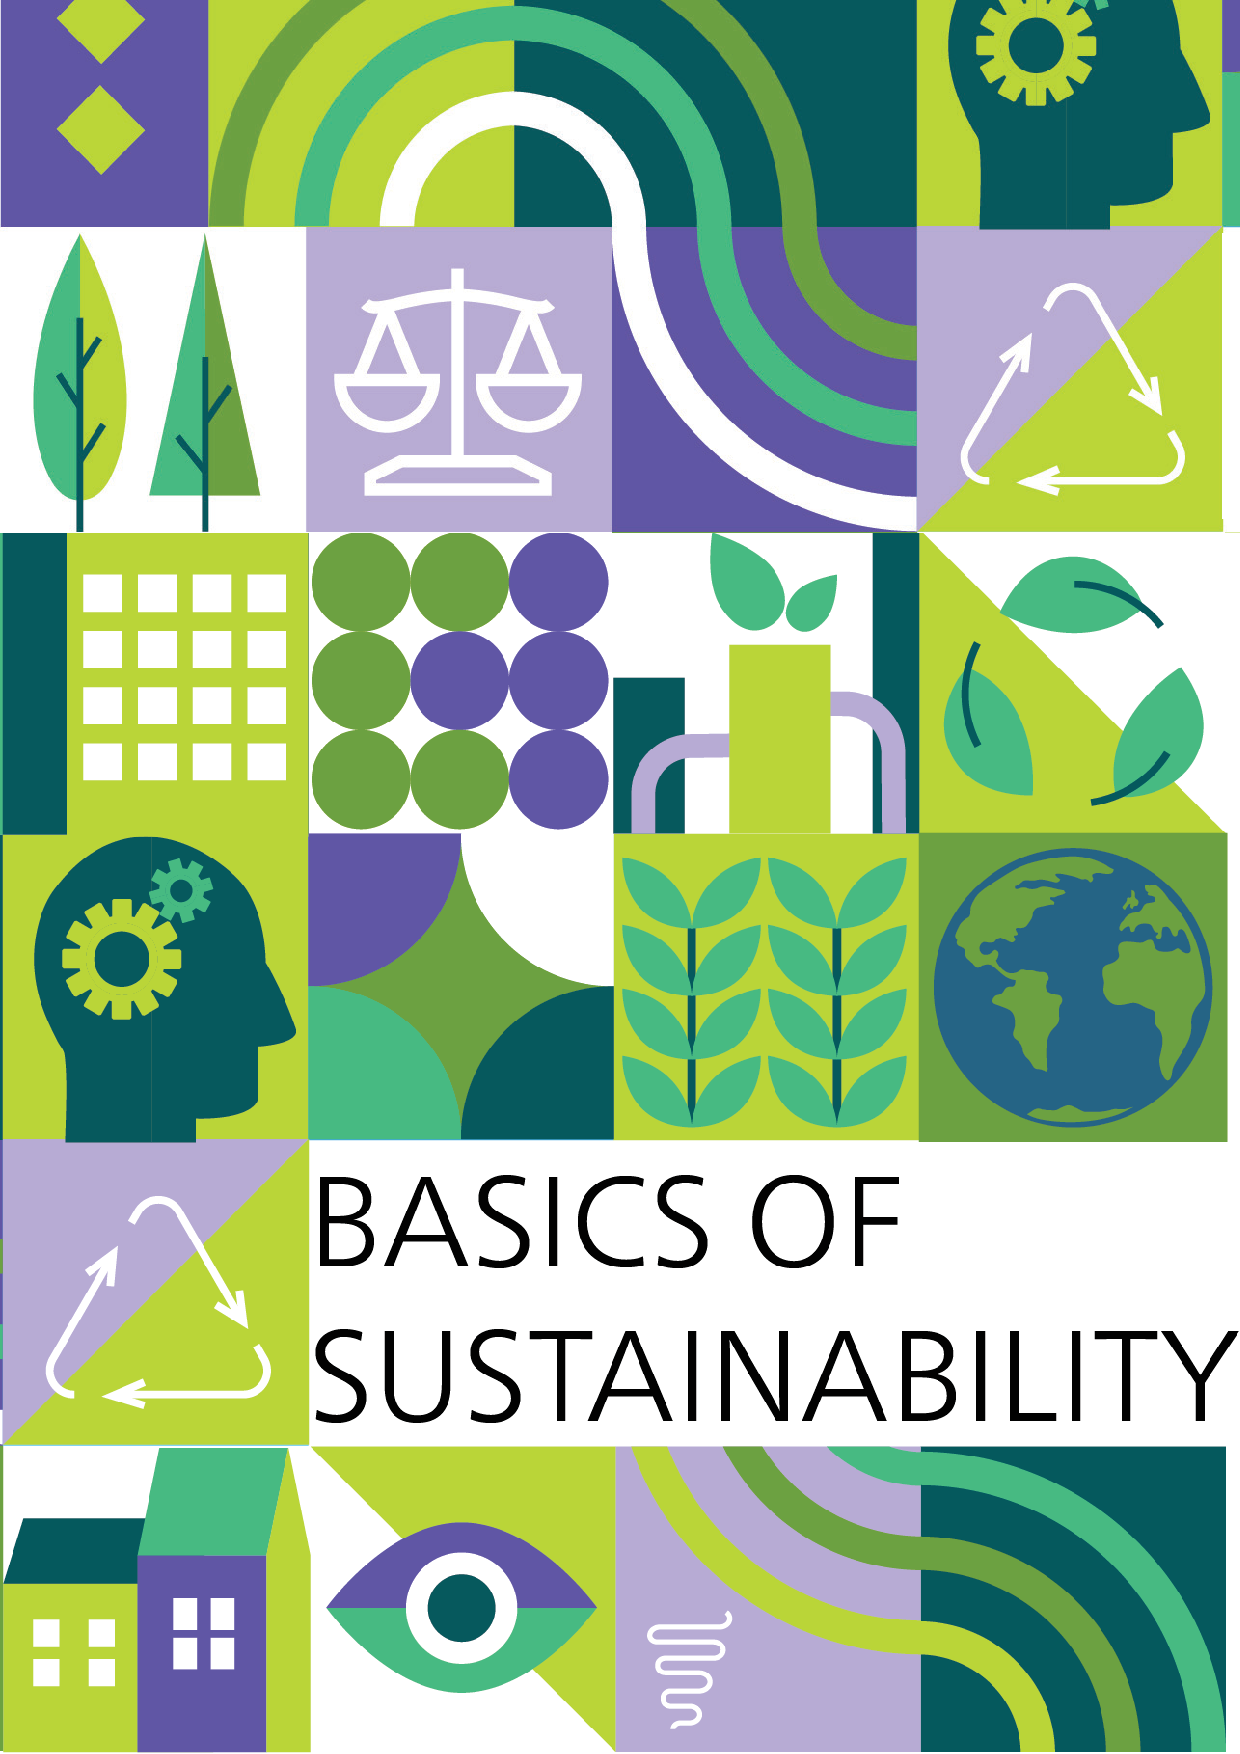
\includepdf[pages=1]{CoverLehrbuch.pdf}

\renewcommand*\contentsname{Inhaltsverzeichnis}
{
\setcounter{tocdepth}{2}
\tableofcontents
}

\bookmarksetup{startatroot}

\chapter*{Disclaimer deutsche
Übersetzung}\label{disclaimer-deutsche-uxfcbersetzung}
\addcontentsline{toc}{chapter}{Disclaimer deutsche Übersetzung}

\markboth{Disclaimer deutsche Übersetzung}{Disclaimer deutsche
Übersetzung}

\begin{tcolorbox}[enhanced jigsaw, arc=.35mm, bottomrule=.15mm, bottomtitle=1mm, breakable, colback=white, colbacktitle=quarto-callout-note-color!10!white, colframe=quarto-callout-note-color-frame, coltitle=black, left=2mm, leftrule=.75mm, opacityback=0, opacitybacktitle=0.6, rightrule=.15mm, title={Hinweis}, titlerule=0mm, toprule=.15mm, toptitle=1mm]

Die Originalfassung dieses Lehrbuch wurde auf Englisch geschrieben und
vollständig editiert
(\url{https://cdeteaching.github.io/Basics-of-sustainability/}). Die
deutsche Version wurde basierend auf dem CDE Style Guide mittels Claude
Code Sonnet 5 (Anthropic) erarbeitet und redigiert durch die
Autorenschaft. Die deutsche Version ist aktuell auf EN V1.3
synchronisiert.

\end{tcolorbox}

\bookmarksetup{startatroot}

\chapter*{Vorwort}\label{vorwort}
\addcontentsline{toc}{chapter}{Vorwort}

\markboth{Vorwort}{Vorwort}

Diese Einführung in die Grundlagen und Herausforderungen der
Nachhaltigen Entwicklung richtet sich an Studierende und Lehrende, die
sich aus unterschiedlichen disziplinären Perspektiven mit den
drängendsten Fragen unserer Zeit befassen. Sie entstand aus dem Wunsch,
ein gemeinsames Verständnis zu fördern -- über Disziplingrenzen hinweg,
in Lehre, Forschung und gesellschaftlicher Praxis.

Die Welt, wie wir sie heute kennen, ist von einer Vielzahl miteinander
verflochtener Krisen geprägt: Klimawandel, Verlust der Biodiversität,
soziale Ungleichheiten, wirtschaftliche Instabilität und politische
Polarisierung -- kurz: eine Polykrise. Diese Herausforderungen sind
weder linear noch einfach zu lösen. Sie verlangen ein tiefgreifendes
Umdenken in unseren wirtschaftlichen, sozialen und ökologischen
Systemen, in unserem Handeln und in unserem Verständnis von Entwicklung
und Fortschritt.

Vor diesem Hintergrund versteht sich dieses Lehrbuch als gemeinsamer
Lernraum: Es bietet einen systematischen Zugang zu zentralen Konzepten,
wissenschaftlichen Perspektiven, normativen Fragen und konkreten
Handlungsfeldern der Nachhaltigen Entwicklung. Ziel ist es dabei nicht
nur, Wissen zu vermitteln, sondern auch die Fähigkeit zur Reflexion, zum
kritischen Denken und zur Kreativität zu fördern.

Dieses Buch entstand im Rahmen der Studienprogramme des Centre for
Development and Environment (CDE) der Universität Bern. Es spiegelt die
langjährige Erfahrung in Forschung und Lehre zur Nachhaltigen
Entwicklung wider und vereint Beiträge aus verschiedenen Disziplinen --
von den Umweltwissenschaften, der Geographie und der Ökonomie bis hin zu
Soziologie, Ethik und Rechtswissenschaften.

Unser besonderer Dank gilt allen Autor*innen, die mit ihrer Expertise,
ihrer Leidenschaft und ihrem Engagement zur Entstehung dieses Buches
beigetragen haben. Ebenso danken wir den Studierenden, deren kritische
Fragen und Perspektiven ein entscheidender Motor für die
Weiterentwicklung der Inhalte sind. Nachhaltige Entwicklung ist
schliesslich nicht nur ein wissenschaftliches, sondern vor allem ein
gesellschaftliches Projekt -- und es beginnt bei der Bildung.

Wir hoffen, dass dieses Buch Ihnen eine solide Grundlage für die eigene
Auseinandersetzung mit Nachhaltigkeit bietet -- und Sie dazu ermutigt,
Verantwortung zu übernehmen und aktiv an der Gestaltung einer gerechten
und nachhaltigen Welt mitzuwirken.

\section*{Zitierhinweis}\label{zitierhinweis}
\addcontentsline{toc}{section}{Zitierhinweis}

\markright{Zitierhinweis}

Bader, C. (Hrsg.). (2025). Grundlagen der Nachhaltigkeit (Version 1.3)
{[}Online-Lehrbuch{]}. CDE, Universität Bern. Abgerufen von
https://cdeteaching.github.io/Basics-of-sustainability/

\textbf{Einzelne Kapitel zitieren:}

Kapitel 1:

Bader, C. (2025). Verständnis und Konzepte der Nachhaltigkeit. In C.
Bader (Hrsg.), Grundlagen der Nachhaltigkeit (Version 1.3)
{[}Online-Lehrbuch{]}. CDE, Universität Bern. Abgerufen von
https://cdeteaching.github.io/Basics-of-sustainability/

Kapitel 2:

Bader, C. (2025). Ansätze zur Nachhaltigkeit. In C. Bader (Hrsg.),
Grundlagen der Nachhaltigkeit (Version 1.3) {[}Online-Lehrbuch{]}. CDE,
Universität Bern. Abgerufen von
https://cdeteaching.github.io/Basics-of-sustainability/

Kapitel 3:

Fitz, J., \& Bader, C. (2025). Ökologische Nachhaltigkeit. In C. Bader
(Hrsg.), Grundlagen der Nachhaltigkeit (Version 1.3)
{[}Online-Lehrbuch{]}. CDE, Universität Bern. Abgerufen von
https://cdeteaching.github.io/Basics-of-sustainability/

Kapitel 4:

Poelsma, F., \& Bader, C. (2025). Soziale Nachhaltigkeit. In C. Bader
(Hrsg.), Grundlagen der Nachhaltigkeit (Version 1.3)
{[}Online-Lehrbuch{]}. CDE, Universität Bern. Abgerufen von
https://cdeteaching.github.io/Basics-of-sustainability/

Kapitel 5:

Bader, C., \& Bezzola, N. (2025). Wirtschaftliche Nachhaltigkeit. In C.
Bader (Hrsg.), Grundlagen der Nachhaltigkeit (Version 1.3)
{[}Online-Lehrbuch{]}. CDE, Universität Bern. Abgerufen von
https://cdeteaching.github.io/Basics-of-sustainability/

\begin{tcolorbox}[enhanced jigsaw, arc=.35mm, bottomrule=.15mm, bottomtitle=1mm, breakable, colback=white, colbacktitle=quarto-callout-note-color!10!white, colframe=quarto-callout-note-color-frame, coltitle=black, left=2mm, leftrule=.75mm, opacityback=0, opacitybacktitle=0.6, rightrule=.15mm, title={Beitragsmatrix (CRediT-Taxonomie)}, titlerule=0mm, toprule=.15mm, toptitle=1mm]

{\def\LTcaptype{none} % do not increment counter
\begin{longtable}[]{@{}
  >{\raggedright\arraybackslash}p{(\linewidth - 6\tabcolsep) * \real{0.2500}}
  >{\raggedright\arraybackslash}p{(\linewidth - 6\tabcolsep) * \real{0.2500}}
  >{\raggedright\arraybackslash}p{(\linewidth - 6\tabcolsep) * \real{0.2500}}
  >{\raggedright\arraybackslash}p{(\linewidth - 6\tabcolsep) * \real{0.2500}}@{}}
\toprule\noalign{}
\begin{minipage}[b]{\linewidth}\raggedright
Name
\end{minipage} & \begin{minipage}[b]{\linewidth}\raggedright
Affiliation
\end{minipage} & \begin{minipage}[b]{\linewidth}\raggedright
ORCID
\end{minipage} & \begin{minipage}[b]{\linewidth}\raggedright
Rollen (CRediT)
\end{minipage} \\
\midrule\noalign{}
\endhead
\bottomrule\noalign{}
\endlastfoot
Christoph Bader & CDE, Universität Bern &
\href{https://orcid.org/0000-0002-8991-353X}{0000-0002-8991-353X} &
Conceptualization, Software, Supervision, Writing - original draft,
Writing -- review \& editing, Project administration \\
Nicolà Bezzola & CDE, Universität Bern & --- & Writing - original draft,
Writing -- review \& editing \\
Juri Fitz & CDE, Universität Bern & --- & Writing - original draft,
Writing -- review \& editing \\
Anna-Lisa Honegger & CDE, Universität Bern & --- & Data curation,
Visualization \\
Helen Pérez & CDE, Universität Bern & --- & Data curation,
Visualization \\
Tina Hirschbühl & CDE, Universität Bern & --- & Writing -- review \&
editing \\
Felix Poelsma & CDE, Universität Bern &
\href{https://orcid.org/0009-0002-0221-6414}{0009-0002-0221-6414} &
Writing - original draft, Writing -- review \& editing \\
\end{longtable}
}

\end{tcolorbox}

\section*{Lesehinweis}\label{lesehinweis}
\addcontentsline{toc}{section}{Lesehinweis}

\markright{Lesehinweis}

Zur besseren Orientierung enthält das Lehrbuch drei Arten von Boxen:

\begin{tcolorbox}[enhanced jigsaw, arc=.35mm, bottomrule=.15mm, bottomtitle=1mm, breakable, colback=white, colbacktitle=quarto-callout-note-color!10!white, colframe=quarto-callout-note-color-frame, coltitle=black, left=2mm, leftrule=.75mm, opacityback=0, opacitybacktitle=0.6, rightrule=.15mm, title={Definitionen}, titlerule=0mm, toprule=.15mm, toptitle=1mm]

Bieten prägnante Definitionen zentraler Begriffe.

\end{tcolorbox}

\begin{tcolorbox}[enhanced jigsaw, arc=.35mm, bottomrule=.15mm, bottomtitle=1mm, breakable, colback=white, colbacktitle=quarto-callout-tip-color!10!white, colframe=quarto-callout-tip-color-frame, coltitle=black, left=2mm, leftrule=.75mm, opacityback=0, opacitybacktitle=0.6, rightrule=.15mm, title={Beispiele und Reflexionsfragen}, titlerule=0mm, toprule=.15mm, toptitle=1mm]

Illustrieren Konzepte anhand konkreter Fälle und regen zur kritischen
Auseinandersetzung mit dem Gelesenen an.

\end{tcolorbox}

\begin{tcolorbox}[enhanced jigsaw, arc=.35mm, bottomrule=.15mm, bottomtitle=1mm, breakable, colback=white, colbacktitle=quarto-callout-caution-color!10!white, colframe=quarto-callout-caution-color-frame, coltitle=black, left=2mm, leftrule=.75mm, opacityback=0, opacitybacktitle=0.6, rightrule=.15mm, title={Weiterführende Literatur}, titlerule=0mm, toprule=.15mm, toptitle=1mm]

Verweise auf ergänzende Materialien.

\end{tcolorbox}

\bookmarksetup{startatroot}

\chapter*{Einleitung}\label{einleitung}
\addcontentsline{toc}{chapter}{Einleitung}

\markboth{Einleitung}{Einleitung}

\begin{figure}

\begin{minipage}[t]{0.50\linewidth}

\begin{figure}[H]

\centering{

\pandocbounded{
\includegraphics[keepaspectratio]{images/cristo.png}}

}

\caption{\label{fig-christo}``Wrapped Globe (Eurasian Hemisphere)'' von
Christo (2019)}

\end{figure}%

\end{minipage}%
%
\begin{minipage}[t]{0.50\linewidth}

\begin{figure}[H]

\centering{

\pandocbounded{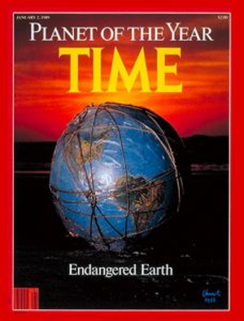
\includegraphics[keepaspectratio]{images/times.png}}

}

\caption{\label{fig-times}``Planet of the Year'', Titelseite des Time
Magazine (1989)}

\end{figure}%

\end{minipage}%

\end{figure}%

Angesichts der wachsenden Herausforderungen der Nachhaltigen Entwicklung
ist Christos und Jeanne-Claudes „Wrapped Globe'' ein kraftvolles Symbol
für die Verantwortung der Menschheit gegenüber unserem Planeten und
seinen Ressourcen. Das Kunstwerk zeigt einen in Klarsichtfolie und ein
filigranes Netz gehüllten Globus. In der Realität sieht sich die Welt
einer \emph{Polykrise} gegenüber -- ein Begriff, der die vielen ernsten
Krisen beschreibt, mit denen unsere Erde konfrontiert ist, darunter
ökologische Krisen, wachsende Ungleichheit und die Folgen der
Covid-19-Pandemie, um nur einige zu nennen. In einer Polykrise sind
Krisen zunehmend miteinander verwoben und verstärken sich gegenseitig
(Tooze 2022). Sie entstehen hauptsächlich durch eine strukturelle
Wachstumsabhängigkeit (gemessen am Bruttoinlandsprodukt, BIP) (Hickel
u.~a. 2022), durch einen Teufelskreis zunehmender Konzentration
wirtschaftlicher und politischer Macht in den Händen weniger (Piketty
2014) sowie durch anhaltende Ungleichheiten zwischen und innerhalb von
Ländern (Chancel u.~a. 2021; Milanović 2016). Dennoch streben wir in
Gesellschaft und Wirtschaft weiterhin nach BIP-Wachstum, um
Arbeitsplätze zu erhalten und zu schaffen, Sozialsysteme zu finanzieren,
Steuereinnahmen zu sichern und die Bedürfnisse von Unternehmen und
Industrien zu erfüllen, die auf Wachstum angewiesen sind. Da diese
Erwartungen zunehmend unrealistisch werden, hat die Idee der Entkopplung
von Wirtschaftswachstum und Ressourcenverbrauch an Zugkraft gewonnen. Es
gibt jedoch keine empirischen Belege dafür, dass dies in dem Ausmass
gelingen kann, das erforderlich wäre, um einen multidimensionalen
ökologischen Kollaps aufzuhalten (Hickel und Kallis 2020; Parrique u.~a.
2019; Wiedmann u.~a. 2020).

\section*{Volle und leere Welt}\label{volle-und-leere-welt}
\addcontentsline{toc}{section}{Volle und leere Welt}

\markright{Volle und leere Welt}

Die Klarsichtfolie und das Netz um Christos Globus stehen damit für die
Vernetzung und gegenseitige Abhängigkeit der verschiedenen Elemente der
Erde und betonen die Notwendigkeit, diese Beziehungen zu erhalten und zu
schützen. Eine ähnliche Idee beschrieb der Ökonom Herman Daly (2015) mit
seinem Konzept der „leeren'' und der „vollen'' Welt. Die leere Welt
beschreibt eine Situation, in der menschliche Aktivitäten und
Ressourcennutzung nur geringfügige Auswirkungen auf die Umwelt haben. In
dieser Welt sind natürliche Systeme noch intakt und unberührt, und die
Ressourcen reichen aus, um menschliche Bedürfnisse zu befriedigen. Im
Gegensatz dazu überlasten in der vollen Welt menschliche Aktivitäten und
Ressourcennutzung die Ökosysteme und belasten die Umwelt. Spätestens
seit dem Zweiten Weltkrieg haben wir eine industrialisierte Gesellschaft
und eine Wachstumswirtschaft verfolgt. Infolgedessen leben wir heute in
einer „vollen'' Welt, in der natürliche Ressourcen knapp sind und das
Gleichgewicht der Ökosysteme bedroht wird.

Dalys Schlüsselerlebnis war die Lektüre von Rachel Carsons Buch
\emph{Silent Spring} im Jahr 1962, das zu einem Leben in Einklang mit
der Natur aufrief. Daly stand dem Hyper-Individualismus wirtschaftlicher
Modelle bereits skeptisch gegenüber, und Carsons Werk verdeutlichte den
Konflikt zwischen einer wachsenden Wirtschaft und einer fragilen Umwelt.
Nach einem Vortrag des Ökonomen Nicholas Georgescu-Roegen über sein
Hauptwerk \emph{The Entropy Law and the Economic Process} (1971)
übernahm Daly die Idee, dass die Wirtschaft eher einer Sanduhr als einem
Pendel ähnelt: Wertvolle Ressourcen werden zu Abfall und gehen damit
weitgehend unwiederbringlich verloren.

Es gibt kein Patentrezept, um der Polykrise entgegenzuwirken und unser
Wirtschafts- und Gesellschaftssystem nachhaltiger zu gestalten. Um zur
Nachhaltigen Entwicklung beizutragen, müssen wir die Ursachen von
Symptomen wie Biodiversitätsverlust oder Klimaerwärmung analysieren und
lernen zu verstehen, wie sie zusammenhängen und interagieren. In unseren
Studienprogrammen werden wir daher aktuelle Probleme und
Herausforderungen wie Klimaerwärmung, Umweltverschmutzung,
Biodiversitätsverlust, soziale Ungleichheit und wirtschaftliche
Ungleichheiten untersuchen, um zu verstehen, wie diesen sowohl auf
lokaler als auch auf globaler Ebene begegnet werden kann.

Dieses Lehrbuch soll Leser*innen dazu anregen, die Rolle von
Einzelpersonen, Gemeinschaften, Unternehmen und Regierungen im Kontext
der Nachhaltigen Entwicklung kritisch zu hinterfragen -- und so Ansätze
zu identifizieren und zu verfolgen, die eine Nachhaltige Entwicklung
fördern. Darüber hinaus möchten wir Zukunftsvisionen entwickeln,
insbesondere in den Masterstudiengängen, die es ermöglichen, sich eine
hohe Lebensqualität in einer nachhaltigen Moderne vorzustellen, und die
einen Wandel der Gegenwart attraktiv statt bedrohlich erscheinen lassen.
Wir möchten eine andere Esskultur, ein anderes Wirtschaftssystem, eine
andere Landnutzung und eine andere Art des Bauens und Wohnens entwerfen.
Um Fortschritte in Richtung Nachhaltigkeit zu erzielen, wird es
entscheidend sein, Akteur*innen einzubinden und die Zusammenarbeit über
Sektoren und Disziplinen hinweg zu fördern. Wie dieses Lehrbuch betonen
wird, werden auch Bildung, Kommunikation und Partizipation unverzichtbar
sein, um eine nachhaltigere Zukunft zu gestalten.

Mit Christos „Wrapped Globe'' vor Augen und Dalys Verständnis der leeren
und der vollen Welt als Grundlage werden wir uns auf eine Reise durch
die vielen Aspekte der Nachhaltigen Entwicklung begeben. Wir hoffen,
dass Sie diese Reise sowohl informativ als auch inspirierend finden und
dass sie Ihnen ein Verständnis für die Dringlichkeit wie auch für die
Chancen der Nachhaltigen Entwicklung vermittelt.

Schliesslich hoffen wir, dass dieses Lehrbuch Leser*innen dazu
inspiriert, über ihre eigene Rolle und Verantwortung in Bezug auf
Nachhaltigkeit nachzudenken, und dass es Sie befähigt, einen Beitrag
dazu zu leisten, dass die Erde auch für künftige Generationen ein
lebenswerter Ort bleibt. Nur gemeinsam können wir die Veränderungen
herbeiführen, die notwendig sind, um eine nachhaltige, gerechte und
umweltfreundliche Welt zu gestalten.

\part{Die Herausforderungen des 21. Jahrhunderts für Nachhaltigkeit
erfassen und verstehen lernen}

\chapter{Verständnisse und Konzepte Nachhaltiger
Entwicklung}\label{verstuxe4ndnisse-und-konzepte-nachhaltiger-entwicklung}

\chapter*{}\label{section}
\addcontentsline{toc}{chapter}{}

\markboth{}{}

\emph{Christoph Bader}

Woher stammen das Konzept, das Leitbild und die Leitprinzipien der
Nachhaltigen Entwicklung? Wie ist das Konzept entstanden, wie hat es
sich entwickelt -- und warum? Die folgenden Ausführungen geben einen
Überblick über die Geschichte der Nachhaltigkeit, den politischen
Hintergrund sowie zentrale Konferenzen und Dokumente. Kurz gesagt: was
hat Nachhaltigkeit zu dem gemacht, was sie heute ist. Es geht darum, das
grosse Ganze zu erkennen. Denn nur wer die Vergangenheit kennt, kann die
Zukunft einschätzen.

Nachhaltigkeit war in den letzten Jahren das Schlagwort schlechthin --
von der Wissenschaft über die Politik und Wirtschaft bis hin zu den
Medien. Der Begriff hatte zunächst eine positive Konnotation, da er mit
dem Langfristigen, dem Beständigen assoziiert wird, und heute gilt
vieles als „nachhaltig``: Kaffee, Unternehmensphilosophien, sogar
Thunfischpizzen. Das sind die Ansprüche einer Konsumgesellschaft mit
einem beträchtlichen -- aber rücksichtslosen -- Appetit auf Überfluss.
Gleich morgens entfernt das Shampoo „nachhaltig`` unsere Schuppen. Dann
fahren wir zur Arbeit in ein Unternehmen, das sich seiner „nachhaltigen
Unternehmensphilosophie`` rühmt, und beim Mittagessen diskutieren wir
über nachhaltige Investitionen. Zuhause schieben wir eine Thunfischpizza
in den Ofen -- natürlich nachhaltig gefischt und produziert, wie es auf
der Packung steht.

Heute ist der Begriff Nachhaltigkeit allgegenwärtig: Er wird im
Zusammenhang mit Energie, Mobilität, Gebäudesanierung, Ernährung,
Bevölkerungsentwicklung, betrieblichem Umweltmanagement und Klimaschutz
verwendet. Auch in Kunst, Kultur, Design und Werbung findet er
Verwendung.

\begin{figure}[H]

\centering{

\pandocbounded{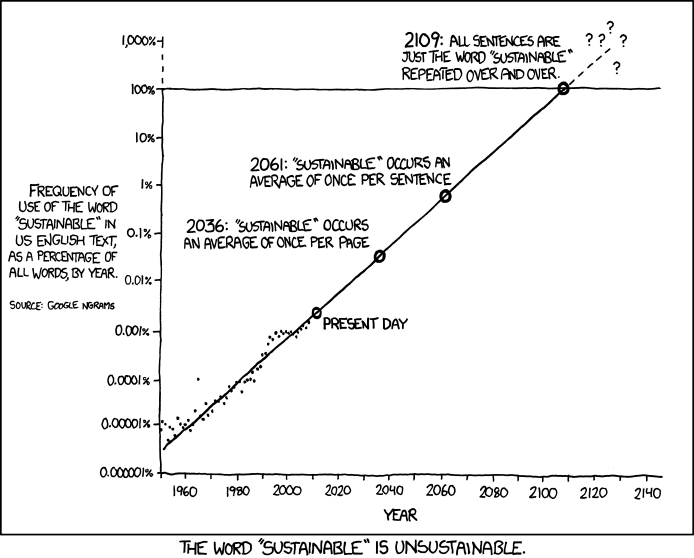
\includegraphics[keepaspectratio]{1_understanding/images/word_sustainable.png}}

}

\caption{\label{fig-word-sustainable}Häufigkeit der Verwendung des
Wortes „sustainable`` in US-amerikanischen Texten, in Prozent aller
Wörter pro Jahr, basierend auf Daten von Google Ngrams. Quelle:
\url{https://xkcd.com/1007/}.}

\end{figure}%

Ist der Begriff „Nachhaltigkeit`` inzwischen so überstrapaziert, dass er
langsam bedeutungslos wird? Selbst wenn dem so wäre, sollten wir
zentrale Begriffe wie diesen nicht leichtfertig aufgeben. So ist es
beispielsweise nach wie vor wichtig, dass Unternehmen eine
Nachhaltigkeitsstrategie haben -- auch wenn viele solcher Strategien
unzureichend sind oder auf Greenwashing hinauslaufen. Wir müssen die
Bedeutung von „Nachhaltigkeit`` klären und diejenigen, die den Begriff
verwenden, zur Rechenschaft ziehen. Unsere Interpretation sollte sich
dabei auf wissenschaftliche Erkenntnisse und historische Entwicklungen
stützen.

Die historischen Vorläufer des in diesem Lehrbuch erläuterten
Nachhaltigkeitsleitbildes sind: Beginn der Diskussion über
Nachhaltigkeit:

\begin{itemize}
\item
  Beginn der Diskussion um Nachhaltigkeit: Carlowitz`
  Waldbewirtschaftungsprinzip 1713
\item
  Zusammenprall von Ökonomie und Ökologie
\item
  Erste und zweite UN-Dekade für Entwicklung
\item
  Grenzen des Wachstums 1972
\item
  Brundtland-Bericht 1987
\item
  Rio Gipfel 1992
\item
  Agenda 21
\item
  Milleniumsziele der UN (MDG)
\item
  Agenda 2030 mit den Nachhaltigkeitszielen (SDG)
\end{itemize}

\section{Ein normatives Konzept}\label{ein-normatives-konzept}

\begin{figure}[H]

\centering{

\pandocbounded{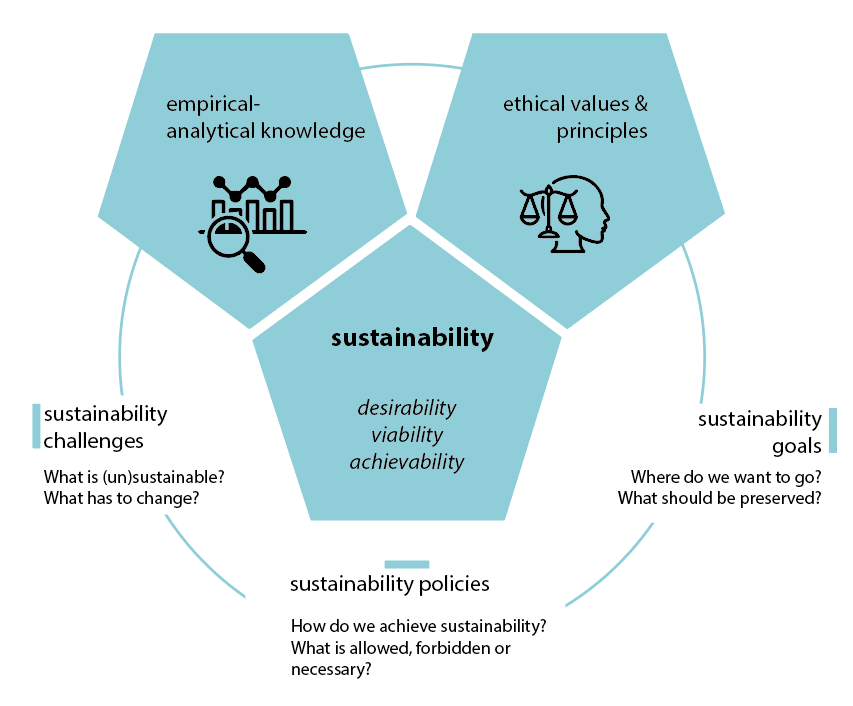
\includegraphics[keepaspectratio]{1_understanding/images/SD_normative.png}}

}

\caption{\label{fig-sd-normative}Nachhaltige Entwicklung als normatives
Konzept. Quelle: Eigene Darstellung.}

\end{figure}%

Um Nachhaltigkeit zu erreichen, brauchen wir \textbf{Nachhaltige
Entwicklung}: einen strategischen Prozess, der Veränderungen in unseren
sozial-ökologischen Systemen und Institutionen erfordert. „Entwicklung''
impliziert eine gezielte Verbesserung, und die ethische Frage, was genau
„besser'' bedeutet, ist dabei zentral. Die Verwendung des Begriffs
„Entwicklung'' wird von einigen kritisiert (z. B. Lang und Mokrani 2013;
Kothari u.~a. 2019), da er häufig mit ungebremstem Wachstum
gleichgesetzt wird. Ungebremstes Wachstum des „ökologischen
Fussabdrucks'' -- des Anteils der Biosphäre, der für menschliche
Produktion, Konsum und Abfall genutzt wird -- ist langfristig nicht
tragfähig. Dennoch gibt es unterschiedliche Interpretationen von
„Entwicklung'', die von Wirtschaftswachstum bis hin zur Verbesserung der
Lebensqualität reichen. Nachhaltige Entwicklung bleibt daher ein
anregendes und umstrittenes Konzept. Nachhaltigkeit und Nachhaltige
Entwicklung spielen im heutigen politischen Diskurs eine zentrale Rolle.
Der Begriff „Nicht-Nachhaltigkeit'' verweist auf Zustände oder
Entwicklungen, die als negativ bewertet werden, während
„Nachhaltigkeit'' einen positiven Zustand beschreibt.

Das Konzept der Nachhaltigen Entwicklung verpflichtet uns auf bestimmte
Werte und Normen, die ethische Ziele und Verhaltensregeln festlegen.
Diese Werte und Normen prägen unsere Vorstellungen davon, was wir als
wünschenswerte oder „positive'' Veränderung betrachten. Ein neutraler
Standpunkt ist nicht möglich, da unsere Wahrnehmungen von einer Vielzahl
von Einflüssen geprägt sind. Unsere persönlichen Erfahrungen, unsere
Erziehung, unser soziales Umfeld und unser kultureller Hintergrund
beeinflussen allesamt, wie wir die Welt sehen und interpretieren --
einschliesslich unserer Vorstellungen davon, was „sein sollte'' und
welche Massnahmen „ergriffen werden sollten''. Ethik spielt eine
zentrale Rolle dabei, wie die aktuelle Situation verbessert werden kann,
um Nachhaltigkeit zu erreichen: Sie definiert normative Ziele und
Grenzen. Nachhaltige Entwicklung ist daher ein konzeptioneller Rahmen,
der stark von ethischen Überlegungen geleitet wird.

Nachhaltigkeitsherausforderungen wie Armutsbekämpfung und Klimawandel
sind deshalb auch ethische Herausforderungen. Die Identifikation von
Situationen als Nachhaltigkeitsprobleme (und damit als „negativ'') und
die Wahl von Lösungen beruhen auf ethischen Werten. Nachhaltigkeitsziele
basieren ebenfalls auf ethischen Werten sowie auf Kenntnissen über
Ursache-Wirkungs-Zusammenhänge. Nachhaltigkeitsfragen werden häufig als
„Wicked Problems'' bezeichnet, da sie komplex und pluralistisch sind.
Der Klimawandel insbesondere wurde als „Super Wicked Problem''
beschrieben, weil Lösungen dringend erforderlich sind, politische
Institutionen häufig unzureichend sind und Entscheidungsprozesse an
Kurzsichtigkeit leiden.

\section{Globale Herausforderungen als Wicked
Problems}\label{globale-herausforderungen-als-wicked-problems}

Mike Hulme, Autor von \emph{Why We Disagree About Climate Change}
(2009), schlägt vor, den Klimawandel als „Wicked Problem'' von enormem
Ausmass und wahrscheinlich langer Dauer zu betrachten. Dieser Ansatz
hilft uns, den Klimawandel nicht als ein zu lösendes Problem zu sehen,
sondern als einen Zustand, in den wir direkt eingebunden sind. Die
Kategorisierung von Problemen als „wicked'' -- also solche, die sich
keiner eindeutigen Lösung erschliessen -- geht auf die
Planungstheoretiker Horst Rittel und Melvin Webber (1973) zurück. Sie
argumentierten, dass Planende mit unvorhersehbarem menschlichem
Verhalten konfrontiert sind und dass manche Probleme zu komplex sind, um
vollständig gelöst zu werden. Einige „Wicked Problems'' werden
möglicherweise nie vollständig gelöst, aber wir können lernen, mit ihnen
umzugehen und uns nicht von ihnen dominieren zu lassen.

\begin{figure}[H]

\centering{

\pandocbounded{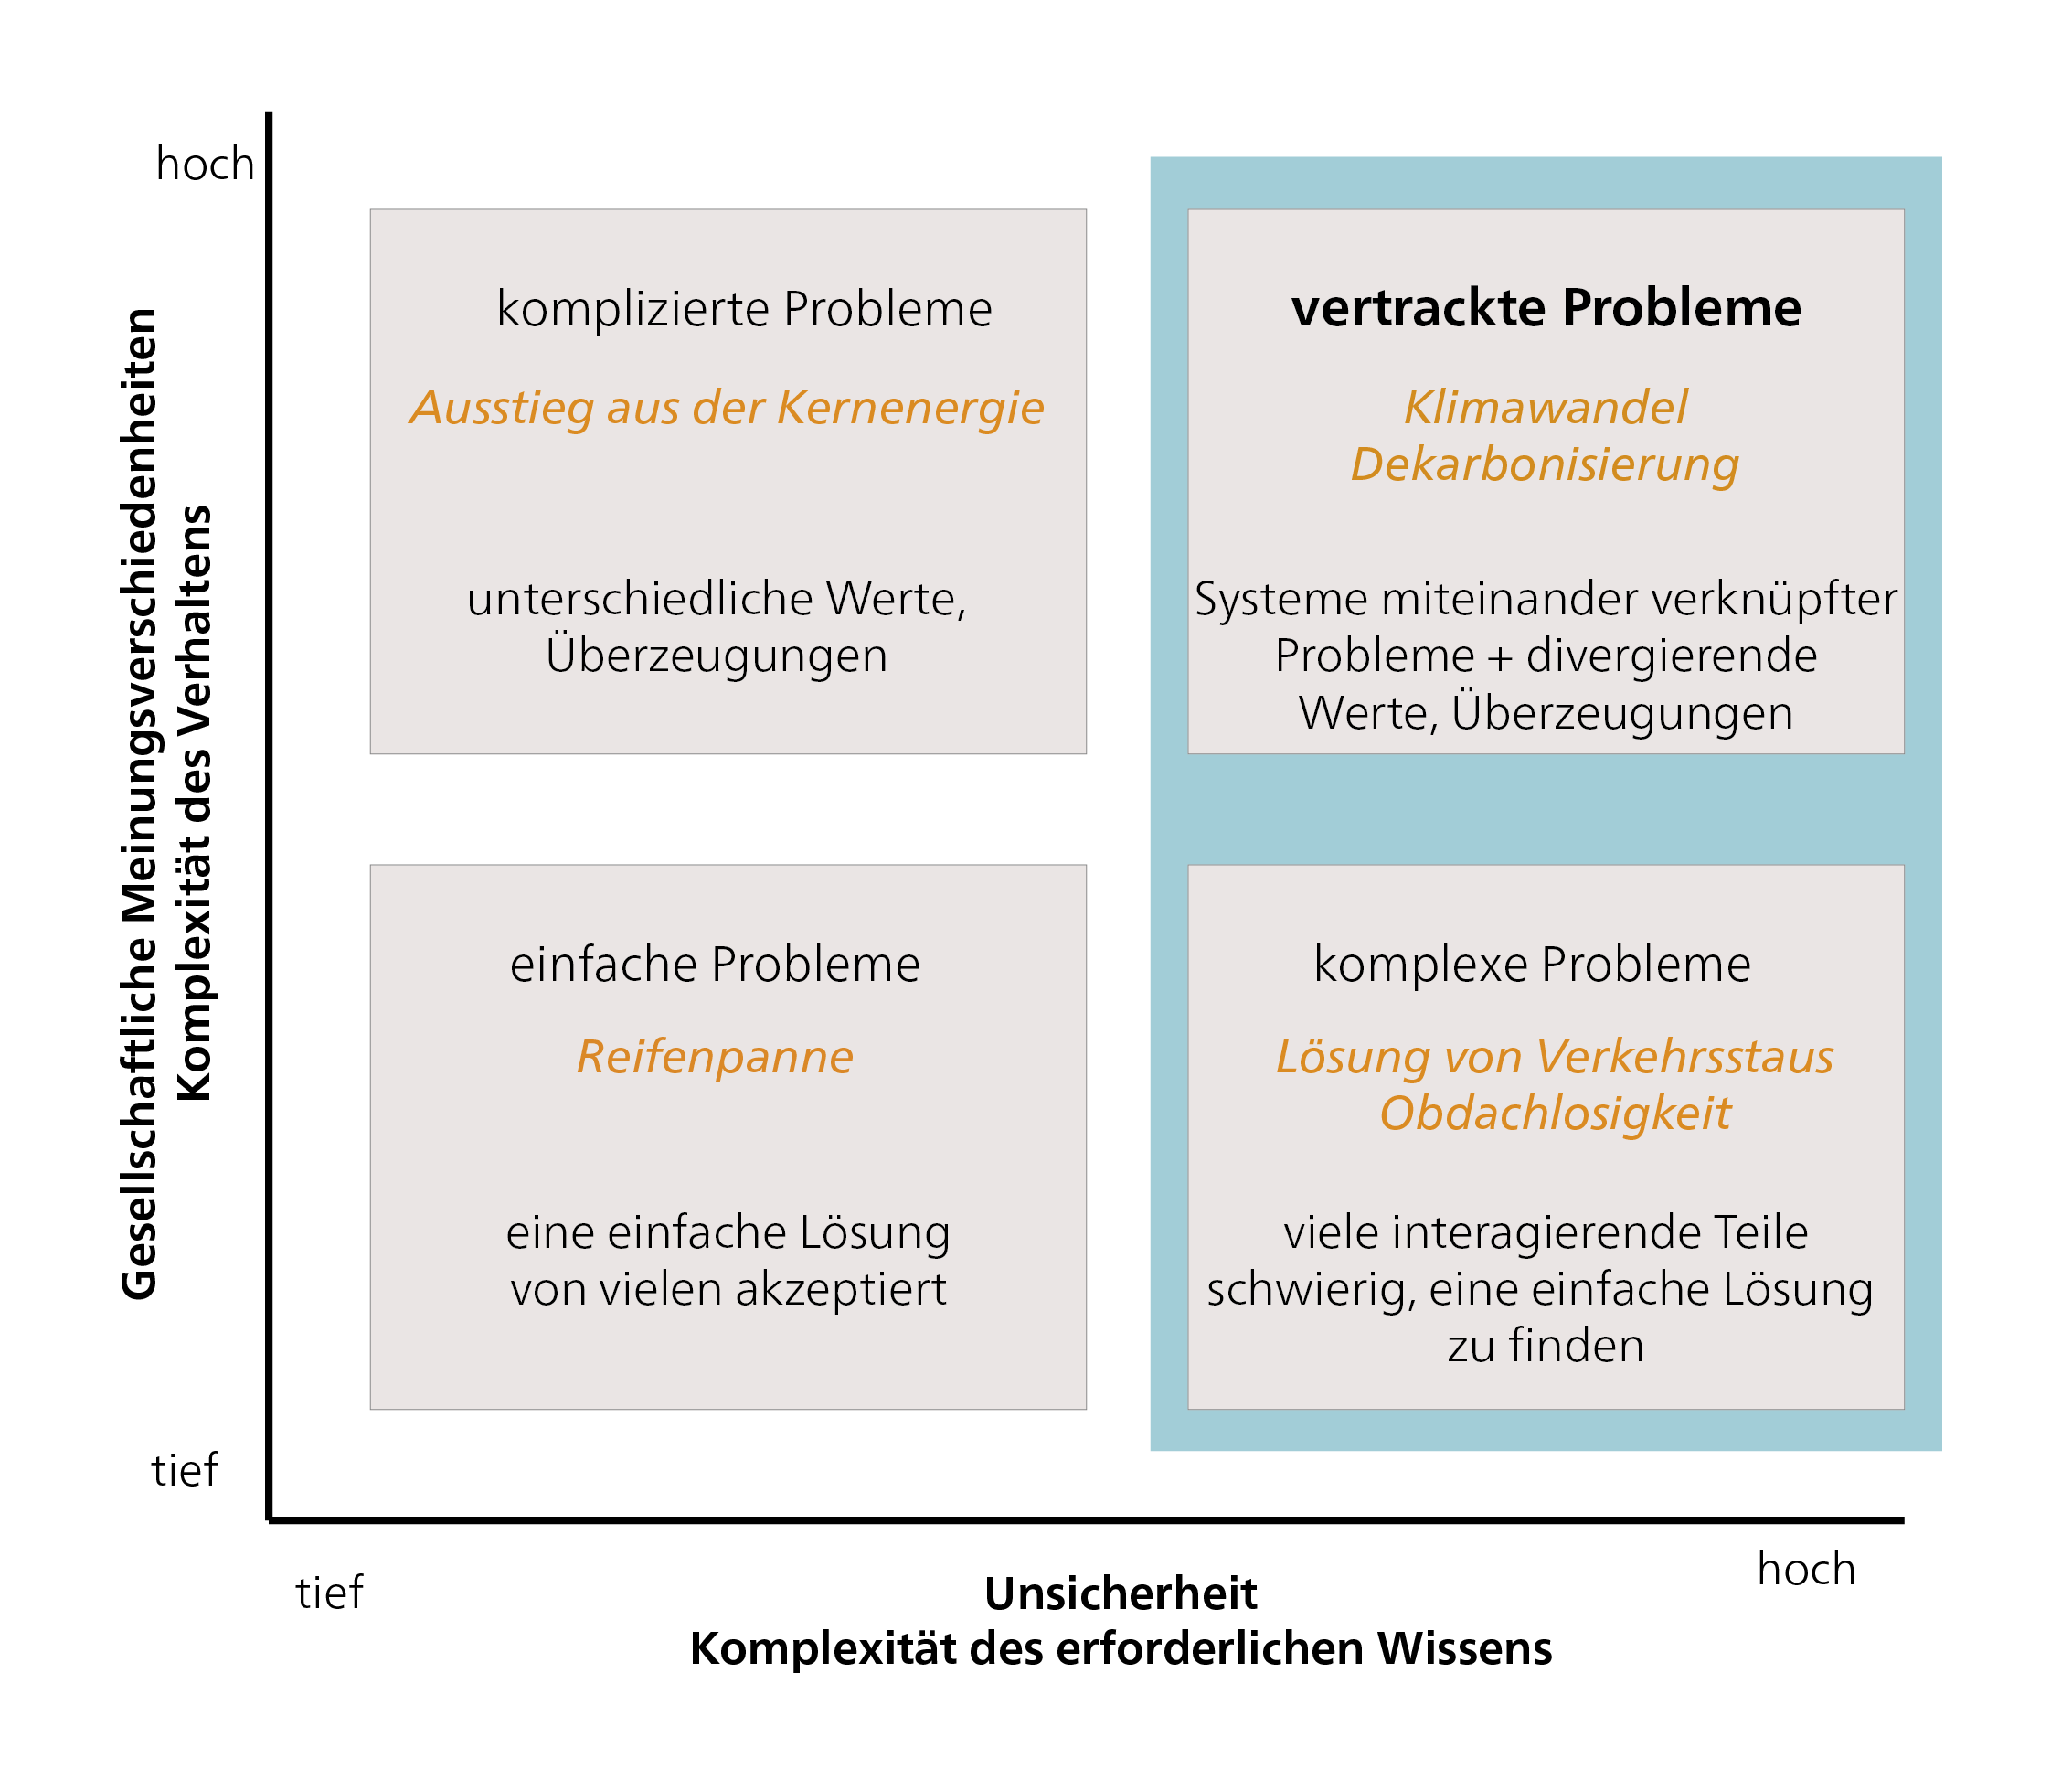
\includegraphics[keepaspectratio]{1_understanding/images/Fig1_3_WickedProblems.png}}

}

\caption{\label{fig-WickedProblems}Nachhaltigkeitsherausforderungen als
Wicked Problems. Quelle: Eigene Darstellung basierend auf Roth, G. L.,
\& Senge, P. M. (1996).}

\end{figure}%

\begin{tcolorbox}[enhanced jigsaw, arc=.35mm, bottomrule=.15mm, breakable, colback=white, colframe=quarto-callout-note-color-frame, left=2mm, leftrule=.75mm, opacityback=0, rightrule=.15mm, toprule=.15mm]

\vspace{-3mm}\textbf{Wicked Problems}\vspace{3mm}

Gemäss Bannink und Trommel (2019) entstehen Wicked Problems an der
Schnittstelle von sachlicher Ungewissheit und einer Heterogenität von
Präferenzen und Interessen. Wicked Problems sind gekennzeichnet durch
(Alford und Head 2017; Rittel und Webber 1973; Sediri u.~a. 2020):

\begin{itemize}
\item
  \textbf{Komplexität}: Wicked Problems sind durch viele miteinander
  verbundene Faktoren und Wechselwirkungen gekennzeichnet. Es gibt keine
  klaren Ursache-Wirkungs-Zusammenhänge, und Veränderungen in einem
  Bereich können unvorhergesehene Auswirkungen in anderen Bereichen
  haben.
\item
  \textbf{Normative Konflikte}: Wicked Problems werden von verschiedenen
  Akteur*innen und Interessengruppen unterschiedlich wahrgenommen und
  interpretiert. Es gibt keine klare Definition oder keinen Konsens
  darüber, was genau das Problem ist oder wie es gelöst werden sollte.
\item
  \textbf{Interdisziplinarität}: Wicked Problems erfordern einen
  interdisziplinären Ansatz, da sie verschiedene Themen, Perspektiven
  und Akteur*innen umfassen. Die Findung einer Lösung erfordert häufig
  die Zusammenarbeit und Koordination verschiedener Disziplinen und
  Expert*innen.
\item
  \textbf{Unsicherheit}: Fehlerhafte, fehlende oder unzugängliche
  Informationen über die Problemsituation und über die Kontinuität der
  Werte der beteiligten Variablen.
\item
  \textbf{Keine eindeutige Lösung}: Wicked Problems lassen sich nicht
  eindeutig lösen. Sie sind dynamisch, verändern sich im Laufe der Zeit
  und erfordern kontinuierliche Anpassung und Iterationen.
\end{itemize}

Beispiele für Wicked Problems sind der Klimawandel, die
Armutsbekämpfung, die globale Gesundheit und die Nachhaltigkeit. Die
Komplexität und das Zusammenspiel verschiedener Faktoren in diesen
Bereichen erschweren es, einfache und eindeutige Lösungen zu finden. Der
Umgang mit Wicked Problems erfordert ein hohes Mass an Reflexion,
Zusammenarbeit und die Anwendung systemischer Denkansätze.

\end{tcolorbox}

Wie haben wir uns in die heutige Situation manövriert, in der Wicked
Problems eine solche Herausforderung für die Nachhaltige Entwicklung
darstellen? In diesem Lehrbuch analysieren und verstehen wir drei
zentrale globale Herausforderungen:

\begin{itemize}
\item
  das Entstehen des menschengemachten Klimawandels;
\item
  die Persistenz globaler Armut und wachsender Ungleichheiten;
\item
  und die Bedrohung durch das Artensterben und die Übernutzung
  natürlicher Ressourcen.
\end{itemize}

Die Debatte über den menschlichen Einfluss auf die globale Erwärmung und
den Klimawandel hat sich seit den Veröffentlichungen des
Intergovernmental Panel on Climate Change (IPCC) intensiviert. Die
treibende Kraft hinter der globalen Erwärmung ist unsere Abhängigkeit
von Öl und anderen fossilen Brennstoffen für Transport, Stromerzeugung,
Landwirtschaft und viele Alltagsprodukte. Ein weiteres Wicked Problem
ist die globale Armut. Obwohl es seit Jahrzehnten globale Bemühungen zur
Armutsbekämpfung gibt, führt die globalisierte Marktwirtschaft in
bestimmten Regionen oft zu zunehmender Armut, und die Kluft zwischen Arm
und Reich scheint sich insgesamt zu vergrössern (Chancel u.~a. 2021).
Hocheinkommensländer haben ihren Wohlstand und ihren Lebensstandard auf
Kosten anderer aufrechterhalten. Dies sind „externalisierte Kosten'', zu
denen auch Umweltschäden gehören. So sind der Reichtum und der
Lebensstandard der Hocheinkommensländer massgeblich verantwortlich für
die Bedrohung des Artensterbens und die Übernutzung natürlicher
Ressourcen (Lessenich 2018). Neben den oben genannten „grossen Drei'' --
Klimawandel, Armut und Biodiversitätsverlust -- gibt es viele weitere
globale Nachhaltigkeitsherausforderungen, wie Entwaldung,
Desertifikation, sinkende Bodenfruchtbarkeit, schwindende Fischbestände,
Umweltverschmutzung, Kriege, Konflikte und zunehmende Migration.

Bei der Analyse dieser umfassenden Herausforderungen müssen wir auch die
zeitliche Dimension berücksichtigen. Im Jahr 2004 wurden erstmals
Grafiken veröffentlicht, die sozioökonomische und Erdsystem-Trends von
1750 bis 2000 abbildeten und einen dramatischen Anstieg zeigten, der
treffend als „Grosse Beschleunigung'' bezeichnet wurde (Steffen u.~a.
2004).

\begin{figure}[H]

\begin{minipage}[t]{0.50\linewidth}

\raisebox{-\height}{

\pandocbounded{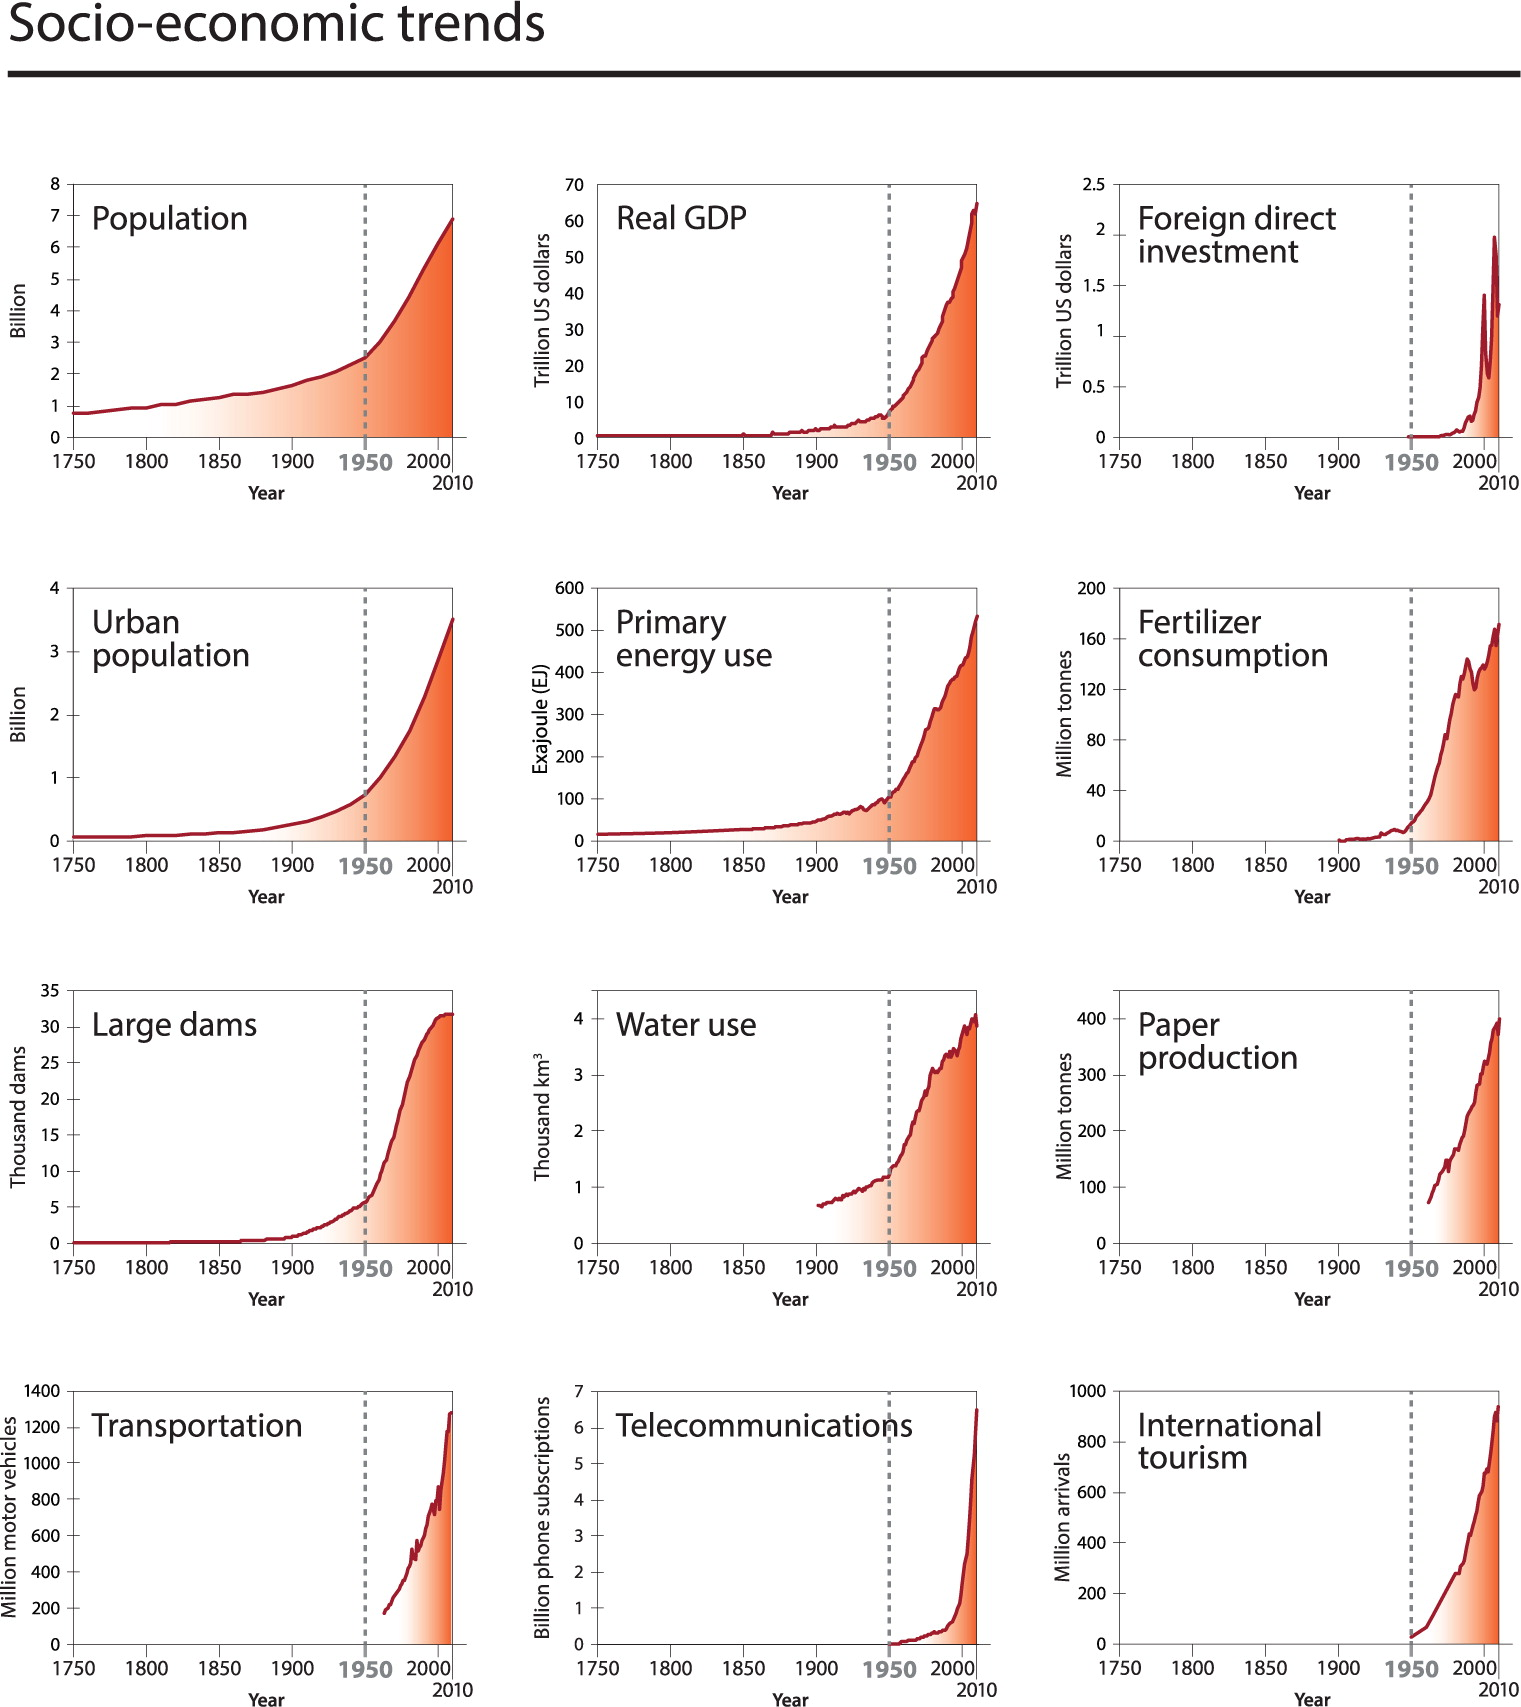
\includegraphics[keepaspectratio]{1_understanding/images/Great-Acceleration_socio-economic_trends.jpg}}

}

\end{minipage}%
%
\begin{minipage}[t]{0.50\linewidth}

\raisebox{-\height}{

\pandocbounded{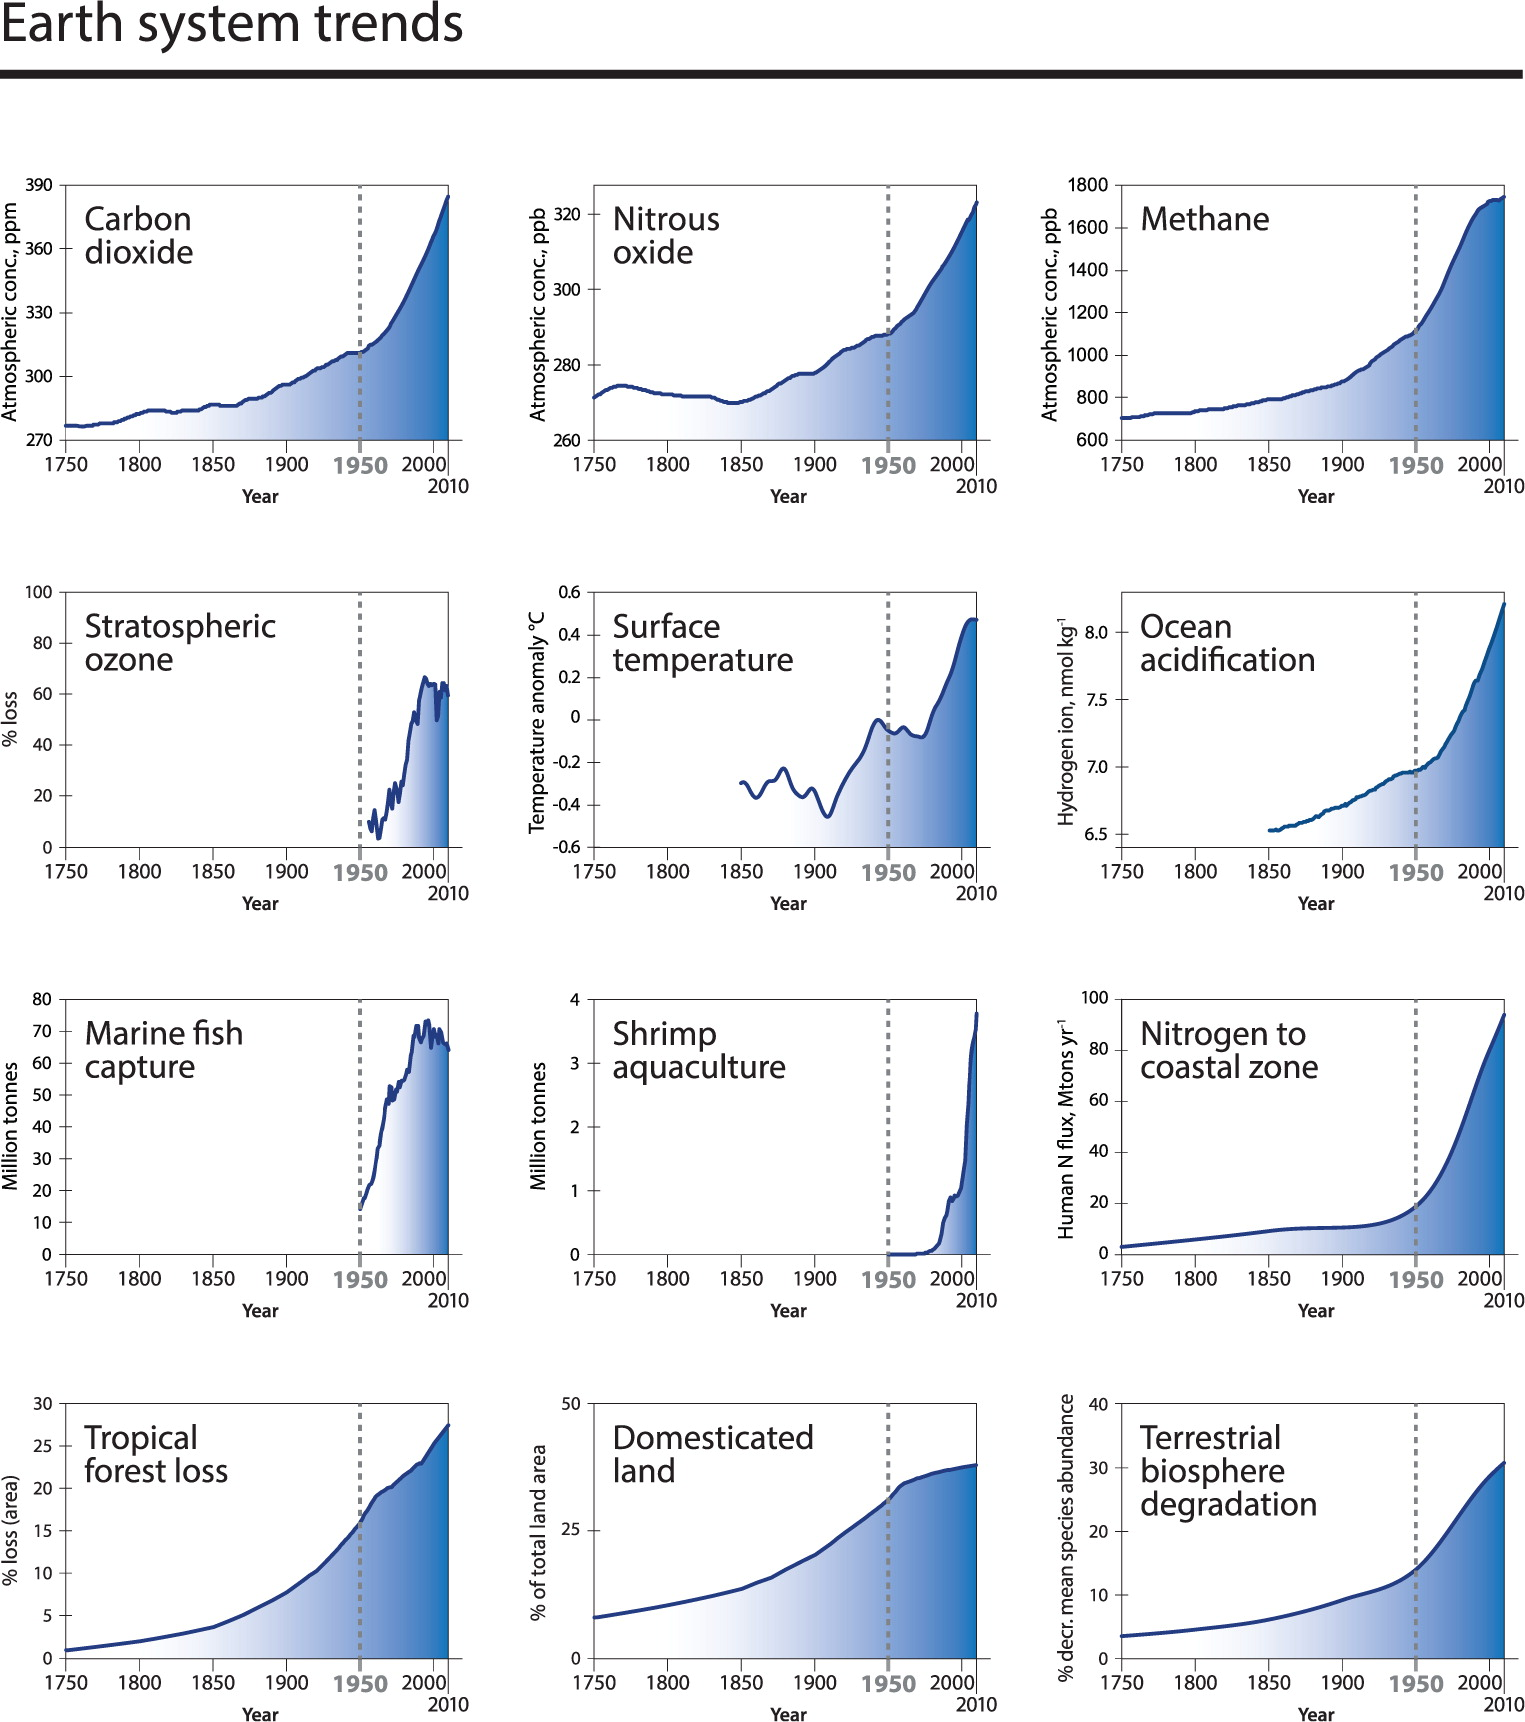
\includegraphics[keepaspectratio]{1_understanding/images/Great-Acceleration_earth-system_trends.jpg}}

}

\end{minipage}%

\caption{\label{fig-acceleration-trends}12 sozioökonomische und 12
Erdsystem-Trends von 1750 bis 2010 sind ein starker Hinweis darauf, dass
das Erdsystem einen neuen Zustand erreicht hat. Quelle:
\url{https://futureearth.org/the-great-acceleration/}.}

\end{figure}%

Die Grosse Beschleunigung beschrieb die exponentiellen
Wachstumsdynamiken, die infolge der Industriellen Revolution entstanden
und zu einem Produktivitätsschub und einem deutlichen Anstieg des
materiellen Wohlstands führten. Gleichzeitig, aber in deutlich
geringerem Ausmass, kam es zu einem massiven Anstieg des
Ressourcenverbrauchs und der Emissionen. Das sozioökonomische Wachstum
ging Hand in Hand mit der Beschleunigung biophysikalischer Trends.
Abbildung~\ref{fig-acceleration-trends} zeigt einige Beispiele wichtiger
biophysikalischer und sozioökonomischer Indikatoren, die alle mit der
Industriellen Revolution zu steigen beginnen. Ab der Mitte des 20.
Jahrhunderts wird der Trend zum exponentiellen Wachstum deutlich.

\begin{tcolorbox}[enhanced jigsaw, arc=.35mm, bottomrule=.15mm, bottomtitle=1mm, breakable, colback=white, colbacktitle=quarto-callout-tip-color!10!white, colframe=quarto-callout-tip-color-frame, coltitle=black, left=2mm, leftrule=.75mm, opacityback=0, opacitybacktitle=0.6, rightrule=.15mm, title={Das Weizenkorn- und Schachbrettproblem: eine Illustration des
exponentiellen Wachstums}, titlerule=0mm, toprule=.15mm, toptitle=1mm]

Das Weizenkorn- und Schachbrettproblem ist ein mathematisches Problem,
das häufig zur Veranschaulichung des exponentiellen Wachstums verwendet
wird. In der Geschichte bittet ein Diener den König, jedes Feld eines
Schachbretts mit Weizenkörnern zu füllen, wobei die Anzahl auf jedem
Feld verdoppelt wird. Das Wachstum beginnt langsam, aber mit jeder
Verdopplung steigt die Anzahl der Körner exponentiell an. Beim 50. Feld
wäre die Anzahl der Reiskörner gross genug, um den 365 Meter hohen
Fernsehturm auf dem Berliner Alexanderplatz zu bedecken. Diese
Geschichte veranschaulicht die immense Kraft des exponentiellen
Wachstums und seine beeindruckenden Ergebnisse. Das Konzept des
exponentiellen Wachstums zu verstehen ist entscheidend für die Analyse
von Phänomenen wie Bevölkerungswachstum, technologischem Fortschritt,
Umweltveränderungen und der Ausbreitung von Krankheiten. Es zeigt, wie
selbst kleine Veränderungen oder Entwicklungen in einem System
erhebliche Auswirkungen haben können. Die Geschichte erinnert uns daran,
dass wir sorgfältig darüber nachdenken müssen, wie wir mit einem solchen
Wachstum umgehen und welche langfristigen Folgen es haben kann.

\end{tcolorbox}

Die Ressourcengewinnung hat in den letzten Jahrzehnten erheblich
zugenommen, von 22 Milliarden Tonnen im Jahr 1970 auf 70 Milliarden
Tonnen im Jahr 2010 (UNEP 2016). Die globale Erwärmung ist ein weiteres
drängendes Problem. Der jüngste IPCC-Bericht (2023) prognostiziert je
nach Szenario und künftigen Emissionen einen Anstieg der globalen
Durchschnittstemperatur zwischen 1,5 und 5,8 Grad Celsius. Ein weiteres
alarmierendes Phänomen ist die Entwaldung. Alle zwei Sekunden wird eine
Waldfläche in der Grösse eines Fussballfeldes abgeholzt -- täglich eine
Fläche von der Grösse New York Citys. Hinzu kommt der Rückgang der
Biodiversität durch das Aussterben von Tier- und Pflanzenarten, der die
ökologische Vielfalt unseres Planeten bedroht.

Die Grosse Beschleunigung (Abbildung~\ref{fig-acceleration-trends})
beschreibt die beobachtbaren und messbaren (negativen) Entwicklungen
wichtiger sozioökonomischer und biophysikalischer Indikatoren seit 1950.
Die Ursachen dieser negativen Entwicklungen können weit entfernt von dem
Ort liegen, an dem die Probleme entstehen oder am deutlichsten werden.
So können beispielsweise Arbeitsplatzverluste in einem Land durch die
Entscheidung eines multinationalen Unternehmens verursacht werden, Teile
seiner Aktivitäten in ein anderes Land zu verlagern, um die Gewinne zu
maximieren. Solche Probleme lassen sich nicht beheben, wenn man nicht
versteht, wie das System -- in diesem Fall die globalisierte Wirtschaft
-- funktioniert. Ähnlich müssen wir die globalen Klimasysteme der Erde
verstehen, um uns vorstellen zu können, welche Folgen die globale
Erwärmung in einem bestimmten Gebiet oder einer bestimmten Region haben
könnte.

Deshalb erfordern viele Methoden und Konzepte der
Nachhaltigkeitswissenschaft systemisches Denken. Ein systemischer
Denkansatz beginnt häufig mit einem Brainstorming, um ein „Rich
Picture'' aller Faktoren zu erstellen, die berücksichtigt werden müssen,
um das aktuelle Verhalten des betreffenden Systems zu verstehen. Im
Falle eines multinationalen Unternehmens, das eine bestimmte
Geschäftseinheit schliesst, wären dies beispielsweise die Faktoren, die
die Entscheidung beeinflussen könnten, bestimmte Geschäftseinheiten
weiterzuführen, auszubauen oder zu schliessen. Obwohl eine erste
Kartierung übermässig komplex oder sogar unübersichtlich wirken kann,
kann die Erstellung eines linearen Flussdiagramms helfen, die Eingangs-
und Einflussströme zu klären. Diese Art der Kartierung kann bereits
Möglichkeiten aufzeigen, die relevanten Einflüsse neu zu bewerten und
das System neu zu gestalten, um unerwünschte Ergebnisse zu vermeiden.
Möglicherweise sind jedoch weitere Arbeiten erforderlich, um
„konzeptionelle Modelle'' des Systems zu entwickeln, die
unvorhergesehene Verbesserungsmöglichkeiten aufzeigen.

Die Einbeziehung des systemischen Denkens in die Methoden und Konzepte
der Nachhaltigkeitswissenschaft ermöglicht es uns, die Komplexität von
Problemen zu bewältigen und fundierte Strategien für eine Nachhaltige
Entwicklung zu entwickeln. Systemisches Denken bietet damit eine
wichtige Grundlage für das Verstehen und Gestalten der verschiedenen
Verständnisse und Konzepte Nachhaltiger Entwicklung, wie das nächste
Kapitel eingehender erläutert.

\section{Nachhaltigkeit: Wann haben wir begonnen, darüber zu
sprechen?}\label{nachhaltigkeit-wann-haben-wir-begonnen-daruxfcber-zu-sprechen}

Im Jahr 1713 zeigte Hans Carl von Carlowitz, der sächsische
Oberberghauptmann, in einem Buch mit dem Titel \emph{Sylvicultura
oeconomica, oder hauswirthliche Nachricht und Naturmässige Anweisung zur
wilden Baum-Zucht} die Notwendigkeit und Möglichkeit einer „nachhaltigen
Forstwirtschaft'' auf. Eine weitere Nachhaltigkeitspioniera war Herzogin
Anna Amalia, die Mutter von Herzog Carl August. In den späten 1700er
Jahren initiierte sie die erste Forstrechtsreform der Welt, die auf eine
kontinuierliche und stetige Holzversorgung abzielte. Zu jener Zeit hatte
Europa einen unstillbaren Hunger nach Materia prima -- den Rohstoffen,
die für den Schiffsbau, den Hausbau sowie zum Kochen und Heizen benötigt
wurden. Diese Nachfrage drohte die Ressourcen zu erschöpfen und ihr
langfristiges Überleben zu gefährden.

Im 18. Jahrhundert befassten sich Gelehrte in Deutschland wie auch in
anderen Teilen Europas mit der Endlichkeit natürlicher Ressourcen.
Anders als von Carlowitz sprach jedoch niemand über Nachhaltigkeit. Ein
wichtiger Aspekt war die Nahrungsversorgung einer wachsenden
Bevölkerung. Vor der Industrialisierung wurde das Wirtschaftswachstum
weitgehend durch die Natur als Produktionsfaktor bestimmt, etwa durch
die Anzahl der gebauten Minen oder Schiffe oder die zur Verfügung
stehende landwirtschaftliche Fläche. Der britische Ökonom Thomas Robert
Malthus warnte jedoch, dass die Nahrungsmittelproduktion nicht mit dem
rasanten Bevölkerungswachstum infolge der Industriellen Revolution
Schritt halten könnte. Malthus glaubte, dass die Bevölkerung
exponentiell wachsen würde, während die Nahrungsmittelproduktion nur
linear zunehmen würde. Obwohl die Malthus'sche These nicht in der von
ihm vorhergesagten dramatischen Weise eingetroffen ist, gilt sein Werk
oft als erste systematische Abhandlung über die Grenzen des Wachstums in
einer endlichen Welt.

Eine Zeit lang gerieten Malthus' Ideen in Vergessenheit, da die
Industrielle Revolution und der Aufstieg des Kapitalismus ein
unbegrenztes Wachstum möglich erscheinen liessen. Von natürlichen
Grenzen war erst wieder Mitte des 20. Jahrhunderts die Rede, als eine
„neo-malthusianische'' Perspektive im Kontext des Club of Rome
(gegründet 1968), der Debatten über planetare Grenzen und der
Wachstumskritik wieder auflebte. Während sich der traditionelle
Malthusianismus auf externe, physische Wachstumsgrenzen konzentriert,
schlägt der Ökologe und Wirtschaftswissenschaftler Giorgos Kallis einen
anderen Ansatz vor. Kallis (2019) plädiert für persönliche Mässigung und
freiwillige Zurückhaltung, eine Lebenseinstellung, die tiefe Wurzeln in
der Romantik und der antiken griechischen Philosophie hat. Er
argumentiert für eine innere Grenze unserer Wünsche, um uns von der
wirtschaftlichen Annahme der Knappheit und der damit verbundenen
Wachstumsversessenheit zu befreien. Kallis erkennt zwar die Realität
äusserer Grenzen an, ist aber der Ansicht, dass diese nicht das
Umweltargument gegen grenzenloses Wachstum dominieren sollten. Kallis
fragt daher, ob es sinnvoll ist, den Klimawandel primär als ein Problem
äusserer Grenzen, der Knappheit oder einer endlichen Atmosphäre zu
rahmen, die nicht mehr unsere Emissionen aufnehmen kann.

In der malthusianischen Logik müssten wir unsere Produktion ständig
steigern, um die Bedürfnisse einer Welt mit Grenzen zu decken. Solange
diese Denkweise anhält, liegt der Fokus darauf, wie wir diese Grenzen
überwinden und die Kapazität des Klimas ausweiten können, eine wachsende
Bevölkerung und ihre Anforderungen aufzunehmen.

\subsection{Das Aufeinanderprallen von Wirtschaft und
Ökologie}\label{das-aufeinanderprallen-von-wirtschaft-und-uxf6kologie}

Ursprünglich war Nachhaltigkeit ein Prinzip der Ressourcenwirtschaft,
das das wirtschaftliche Ziel der langfristigen Maximierung der
Waldnutzung mit ökologischen Bedingungen für das Nachwachsen verband. Im
19. Jahrhundert entstand das Konzept des „ewigen Waldes'' mit dem Ziel,
die Übernutzung zu beenden und eine langfristige Versorgung mit Holz als
wichtigem Rohstoff sicherzustellen. Forstwissenschaftler wie Heinrich
Cotta entwickelten mathematische Methoden zur Berechnung von
Holzvorräten und -wachstum. Im Laufe der Zeit verlagerte sich der Fokus
jedoch auf die reine Ertragstheorie, die kurze Umtriebszeiten,
ertragsreiche Monokulturen und die Maximierung finanzieller Vorteile in
den Vordergrund stellte. Plötzlich ging es um den höchstmöglichen
direkten Geldertrag statt um einen gleichbleibend hohen Holzertrag.
Natürliche Kreisläufe wurden durch kapitalistische Dynamiken ersetzt;
der Tauschwert verdrängte den Gebrauchswert. Dies entwertete das
Leitbild der Nachhaltigkeit, und es dauerte über hundert Jahre -- bis in
die 1960er und 1970er Jahre --, bis die wissenschaftlichen Disziplinen
Ökologie und Nachhaltigkeit wieder an Bedeutung gewannen.

\subsection{Club of Rome und Die Grenzen des
Wachstums}\label{club-of-rome-und-die-grenzen-des-wachstums}

\begin{quote}
„Wenn die gegenwärtigen Wachstumstrends in der Weltbevölkerung,
Industrialisierung, Umweltverschmutzung, Nahrungsmittelproduktion und
Ressourcenverbrauch unverändert anhalten, werden die Grenzen des
Wachstums auf diesem Planeten irgendwann innerhalb der nächsten hundert
Jahre erreicht sein.'' (Meadows u.~a. 1972, pp.~23)
\end{quote}

\begin{figure}[H]

\centering{

\pandocbounded{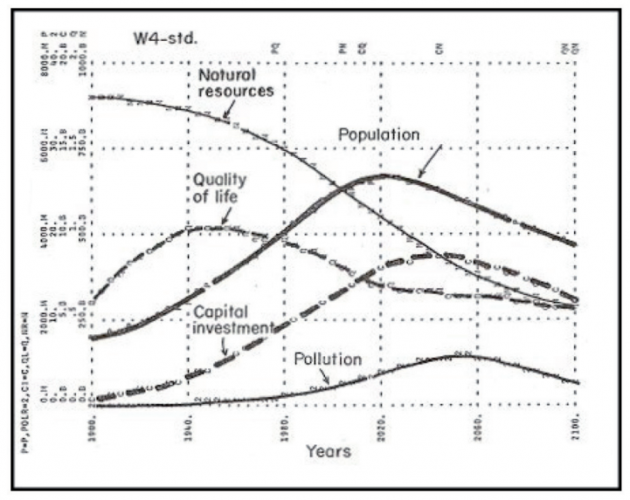
\includegraphics[keepaspectratio]{1_understanding/images/Basic-model.png}}

}

\caption{\label{fig-basic-model}Das „Grundmodell'' der am MIT
durchgeführten Simulation, veröffentlicht im Herbst 1970. Quelle:
\url{https://donellameadows.org/}.}

\end{figure}%

Im Jahr 1972 veröffentlichte der Club of Rome einen Bericht mit dem
Titel \emph{Die Grenzen des Wachstums}, der ein weitaus umfassenderes
Verständnis von „Nachhaltigkeit'' einführte. Wissenschaftler*innen
begannen, einen globalen Gleichgewichtszustand, eine Homöostase, zu
fordern, der nur durch koordiniertes internationales Handeln möglich
wäre. Sie integrieren wirtschaftliche, ökologische und soziale Aspekte
der Nachhaltigkeit und nutzen das Modell der Dynamik komplexer Systeme
(„Systemdynamik''), um die Welt zu verstehen. Sie berücksichtigen die
Wechselwirkungen zwischen Bevölkerungsdichte, Nahrungsressourcen,
Energie, Materialien, Kapital, Umweltzerstörung und Landnutzung.
Computersimulationen verschiedener Szenarien zeigen ähnliche Ergebnisse:
einen katastrophalen Rückgang der Weltbevölkerung und des
Lebensstandards innerhalb von 50 bis 100 Jahren, wenn die aktuellen
Trends anhalten. Das Problem ressourcen- und emissionsintensiver
Industriegesellschaften liegt darin, dass Wachstum nicht linear, sondern
exponentiell verläuft. Langfristig führt diese Art von Wachstum zum
Kollaps. Und einen ökologischen Kollaps könne nur eine Kurskorrektur
verhindern, so der Bericht.

Der \emph{Meadows-Bericht}, wie er auch bekannt ist, wurde wegen seiner
Vorhersagen und Methoden scharf kritisiert. Einige Kritiker*innen
argumentierten, das systemdynamische Modell sei zu vereinfacht und
berücksichtige wichtige Faktoren wie Technologie und Innovation nicht
ausreichend. Andere sagten, die Anpassungsfähigkeit des Menschen und die
Möglichkeit politischer Lösungen und Veränderungen seien zu wenig
beachtet worden. Wiederum andere kritisierten die als malthusianisch
bezeichnete Weltsicht und eine pessimistische Zukunftssicht. Trotz
dieser Kritik löste der Bericht eine wichtige Debatte über
Nachhaltigkeit und die Notwendigkeit des Umweltschutzes aus.

Ein Jahr später veröffentlichte E.F. Schumacher \emph{Small is
Beautiful: Economics as if People Mattered} (1973). Schumacher
hinterfragte die vorherrschende Vorstellung von grenzenlosem
Wirtschaftswachstum und technologischem Fortschritt. Stattdessen
plädierte er für eine nachhaltige, menschenzentrierte Wirtschaft, die
lokale Gemeinschaften und die Umwelt respektiert. Schumacher
argumentierte, dass eine dezentralisierte Wirtschaft, die auf
menschlichen Werten und nicht nur auf Profit basiert, eine bessere
Zukunft für alle schaffen würde. Er betonte auch die Bedeutung von
Bildung und kultureller Entwicklung für die Schaffung einer nachhaltigen
Gesellschaft.

\section{Von der Entwicklungsdebatte zur
Nachhaltigkeitsdebatte}\label{von-der-entwicklungsdebatte-zur-nachhaltigkeitsdebatte}

Die zunehmende Luft- und Wasserverschmutzung trug dazu bei, dass
Umweltthemen in der Politik und den Medien an Bedeutung gewannen.
Greenpeace wurde 1971 gegründet. In den 1960er und 1970er Jahren
erforschten Paul Crutzen und sein Forschungsteam die Auswirkungen von
Stickoxiden auf die Ozonschicht und sagten voraus, dass diese Schicht
durch menschengemachte FCKW stark geschädigt werden würde. Der Einsatz
von FCKW in Kühlschränken und Klimaanlagen wurde daraufhin verboten. Als
Reaktion auf die wachsende Bedeutung von Umweltfragen organisierte die
UNO 1972 in Stockholm die erste grosse Umweltkonferenz überhaupt. Die
als UNO-Konferenz über die menschliche Umwelt bekannte Veranstaltung
führte zur Gründung des Umweltprogramms der Vereinten Nationen (UNEP)
und unabhängiger Umweltministerien in vielen Ländern.

\begin{figure}[H]

\centering{

\pandocbounded{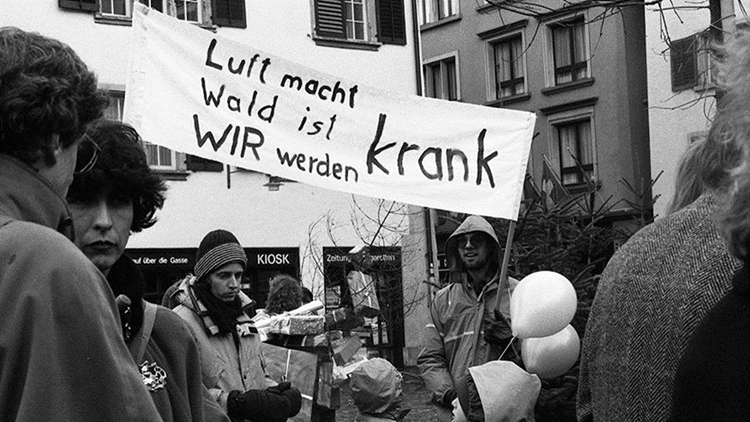
\includegraphics[keepaspectratio]{1_understanding/images/Demonstration_air-pollution_Zürich.png}}

}

\caption{\label{fig-demo-air-poll}Demonstration gegen Luftverschmutzung,
Zürich, Dezember 1986. Quelle: Schweizerisches Sozialarchiv/Gertrud
Vogler.}

\end{figure}%

Das Aufkommen von Umweltproblemen in den 1970er und 1980er Jahren fiel
mit den ersten „Entwicklungskrisen'' nach dem Zweiten Weltkrieg
zusammen. In jenen Tagen sprach man noch von „unterentwickelten
Ländern''. Nach dem Erfolg des Marshallplans beim Wiederaufbau Europas
nach dem Zweiten Weltkrieg wurde angenommen, dass ähnliche Programme,
wie ein Marshallplan für Afrika, zu einem raschen Aufholprozess in der
sozioökonomischen Entwicklung der armen Länder des Globalen Südens
führen würden. Doch die 1970er und 1980er Jahre zeigten das Gegenteil.
Selbst Vorzeigeländer wie Mexiko und Brasilien erlagen Schuldenkrisen
und demonstrierten, dass die Erreichung sozioökonomischer Entwicklung
und die Überwindung von Armut weitaus komplexere Herausforderungen
waren.

Von da an war klar, dass Entwicklungs- und Umweltfragen auf
zwischenstaatlicher Ebene gemeinsam betrachtet werden mussten. Im Jahr
1983 setzte die UNO eine Weltkommission für Umwelt und Entwicklung ein,
die von der norwegischen Premierministerin Gro Harlem Brundtland
geleitet wurde.

\subsection{Brundtland-Kommission}\label{brundtland-kommission}

Gro Harlem Brundtland ernannte 22 Kommissionsmitglieder, von denen drei
Viertel aus dem Globalen Süden stammten. In dieser Zeit begann die
Sowjetunion, die mit wirtschaftlicher Stagnation zu kämpfen hatte, ihren
politischen Kurs zu ändern. Da das Wettrüsten mit den USA zu einem
erheblichen Haushaltsdefizit beigetragen hatte, leitete Michail
Gorbatschow, der neu ernannte Generalsekretär der Kommunistischen Partei
der Sowjetunion, umfassende Reformen ein. Gleichzeitig begann sich ein
neues Weltbild und ein globales Bewusstsein herausuzubilden. Vor diesem
Hintergrund wurde die Brundtland-Kommission mit der Aufgabe betraut,
einen Bericht über die Perspektiven einer globalen, nachhaltigen und
umweltverträglichen Entwicklung bis zum Jahr 2000 und darüber hinaus zu
erarbeiten. Der 1987 vorgelegte Bericht trug den Titel \emph{Our Common
Future} -- häufig auch als \emph{Brundtland-Bericht} bezeichnet.

Der Brundtland-Bericht stellte fest, dass die globalen Umweltprobleme
hauptsächlich auf nicht nachhaltigen Konsum- und Produktionsmustern im
Norden und auf schwerer Armut im Süden beruhen. Die Übernutzung der
Natur und die Erschöpfung natürlicher Ressourcen verschärften
Ungleichheiten (bei Einkommen und Vermögen), steigerten die absolute
Armut und stellten eine Bedrohung für Frieden und Sicherheit dar. Der
Bericht bemühte sich um eine faire und gerechte Definition von
Nachhaltigkeit:

\begin{quote}
„Nachhaltige Entwicklung ist eine Entwicklung, die die Bedürfnisse der
Gegenwart befriedigt, ohne die Möglichkeiten zukünftiger Generationen zu
gefährden, ihre eigenen Bedürfnisse zu befriedigen.'' (WCED 1987a)
\end{quote}

Diese Definition brachte eine ethische Perspektive in die
Nachhaltigkeitsdebatte ein und stellte das Prinzip der Verantwortung
gegenüber den heutigen und zukünftigen Generationen in den Mittelpunkt.
Durch die Fokussierung auf menschliche Bedürfnisse nahm die
Brundtland-Kommission eine anthropozentrische Position ein. Sie
identifizierte drei Schlüsselprinzipien für die Analyse von Problemen
und die Ausrichtung von Handlungen: eine globale Perspektive, die
Verflechtung von Umwelt und Entwicklung sowie das Streben nach
Gerechtigkeit und Chancengleichheit. Das Konzept der
Gerechtigkeit/Chancengleichheit wurde in zwei verschiedene Perspektiven
unterteilt:

\begin{enumerate}
\def\labelenumi{\arabic{enumi}.}
\tightlist
\item
  Die intergenerationelle Perspektive: Verantwortung gegenüber künftigen
  Generationen.
\item
  Die intragenerationelle Perspektive: Verantwortung gegenüber den heute
  lebenden Menschen, insbesondere in Entwicklungsländern, und die
  Sicherstellung von Chancengleichheit innerhalb der Länder.
\end{enumerate}

\begin{tcolorbox}[enhanced jigsaw, arc=.35mm, bottomrule=.15mm, bottomtitle=1mm, breakable, colback=white, colbacktitle=quarto-callout-note-color!10!white, colframe=quarto-callout-note-color-frame, coltitle=black, left=2mm, leftrule=.75mm, opacityback=0, opacitybacktitle=0.6, rightrule=.15mm, title={Nachhaltigkeit und Nachhaltige Entwicklung}, titlerule=0mm, toprule=.15mm, toptitle=1mm]

Die Konzepte „Nachhaltigkeit'' und „Nachhaltige Entwicklung''
unterscheiden sich in ihrem Fokus. Nachhaltigkeit ist statisch; sie
betont einen beständigen Zustand, während Nachhaltige Entwicklung der
dynamische Prozess ist, diesen Zustand zu erreichen -- sie impliziert
Bewegung und verweist auf etwas Werdendes.

\end{tcolorbox}

\section{Von Rio 1992 bis heute}\label{von-rio-1992-bis-heute}

Nach dem Aufruf des Brundtland-Berichts zum internationalen Handeln
richtete sich der Fokus darauf, Forderungen und Vorschläge in
verbindliche Verträge und Konventionen umzusetzen. Die UNO wählte eine
Konferenz als Instrument dafür, genau 20 Jahre nach der Stockholmer
Konferenz von 1972, der ersten globalen Umweltkonferenz. Die im Juni
1992 in Rio de Janeiro, Brasilien, abgehaltene UNO-Konferenz für Umwelt
und Entwicklung -- auch als Erdgipfel bekannt -- war bis dahin die
grösste internationale Konferenz mit Delegierten aus über 170 Nationen.

Der Rio-Erdgipfel verabschiedete folgende fünf Dokumente:

\begin{itemize}
\tightlist
\item
  Eine Walderklärung, die auf die ökologische Bewirtschaftung und den
  Schutz der Wälder der Welt abzielt;
\item
  Eine Klimaschutzkonvention, die die Staaten verpflichtet, die
  Treibhausgasemissionen weltweit auf das Niveau von 1990 zu reduzieren;
\item
  Eine Biodiversitätskonvention zur Bekämpfung des Rückgangs der
  Biodiversität durch völkerrechtlich verbindliche Massnahmen;
\item
  Die Rio-Erklärung zu Umwelt und Entwicklung; sowie Agenda 21, das
  bekannteste der fünf Abkommen, wonach die nationalen Regierungen für
  die Umsetzung des Nachhaltigkeitsmodells in ihren Ländern
  verantwortlich sind.
\end{itemize}

Die Rio-Erklärung zu Umwelt und Entwicklung betont, dass ein
langfristiger wirtschaftlicher Fortschritt nur mit einem Ökosystemansatz
möglich ist. Dies wiederum erfordert eine neue und gerechte globale
Partnerschaft zwischen Regierungen, Bevölkerung und wichtigen
gesellschaftlichen Gruppen. Um dies zu erreichen, sind internationale
Abkommen zum Schutz der Umwelt und des Entwicklungssystems notwendig.
Die Rio-Erklärung legte wichtige Prinzipien der Nachhaltigen Entwicklung
fest, darunter das Vorsorgeprinzip und das Verursacherprinzip. Prinzip
15 beispielsweise besagt: „Zum Schutz der Umwelt werden die Staaten
entsprechend ihren Möglichkeiten den Vorsorgeansatz weitgehend anwenden.
Wenn ernste oder irreversible Schäden drohen, darf der Mangel an
vollständiger wissenschaftlicher Gewissheit nicht als Grund für die
Aufschiebung kosteneffizienter Massnahmen zur Verhinderung von
Umweltschäden herangezogen werden.'' (UN 1992b)

Im Dezember 1992 wurde die Kommission für Nachhaltige Entwicklung (CSD)
gegründet, um eine wirksame Nachbereitung des Gipfels zu gewährleisten.

\subsection{Agenda 21: Global denken -- lokal
handeln}\label{agenda-21-global-denken-lokal-handeln}

Die Agenda 21, die 40 Kapitel umfasst, behandelt alle kritischen
Politikbereiche und Massnahmen für eine Nachhaltige Entwicklung. Laut
Präambel „wird die Integration von Umwelt- und Entwicklungsanliegen und
ihre stärkere Berücksichtigung zur Erfüllung grundlegender Bedürfnisse,
zu einem verbesserten Lebensstandard für alle, zu besser geschützten und
bewirtschafteten Ökosystemen und zu einer sichereren, wohlhabenderen
Zukunft führen. Keine Nation kann dies allein erreichen; aber gemeinsam
können wir es -- in einer globalen Partnerschaft für eine Nachhaltige
Entwicklung.'' (UN CSD 1992)

\subsection{Die Millenniums-Entwicklungsziele
(MDGs)}\label{die-millenniums-entwicklungsziele-mdgs}

Die Grundprinzipien der Agenda 21 -- Stärkung der Rolle der Frauen,
Umweltschutz und Förderung einer gerechten und inklusiven Gesellschaft
-- legten den Grundstein für die Millenniums-Entwicklungsziele (MDGs).
Die von der UNO im Jahr 2000 verabschiedeten MDGs umfassten acht
spezifische Ziele, die bis 2015 erreicht werden sollten. Obwohl nicht
alle diese Ziele erreicht wurden, machten die MDGs das Bewusstsein für
die Notwendigkeit einer Nachhaltigen Entwicklung erheblich stärker. Die
MDGs wurden von den Zielen für Nachhaltige Entwicklung (SDGs) abgelöst,
die die UNO im Jahr 2015 verabschiedete.

\subsection{Rio+20}\label{rio20}

Die UNO-Konferenz für Nachhaltige Entwicklung, oder Rio+20, fand 2012 in
Rio de Janeiro statt, 20 Jahre nach dem historischen Erdgipfel von 1992,
auf dem die Agenda 21 verabschiedet worden war. Das Hauptziel von Rio+20
war die Bekräftigung des globalen politischen Engagements für
Nachhaltige Entwicklung. Die Teilnehmenden, darunter
Regierungsvertreter*innen sowie Repräsentant*innen aus Zivilgesellschaft
und Privatwirtschaft, diskutierten ein breites Themenspektrum, darunter
Armutsbekämpfung, Umweltschutz, nachhaltige Energie,
Ernährungssicherheit und Ressourcenmanagement. Das wichtigste Ergebnis
des Gipfels war die Annahme einer Erklärung mit dem Titel „The Future We
Want''. Diese Erklärung erneuerte das Bekenntnis der internationalen
Gemeinschaft zur Nachhaltigen Entwicklung und zu den Rio-Prinzipien und
früheren Aktionsplänen und legte weitere Massnahmen zur Erreichung
dieser Ziele fest. Darüber hinaus ebnete Rio+20 den Weg für einen
universellen Entwicklungsrahmen zur Festlegung globaler
Nachhaltigkeitsziele und -prioritäten über 2015 hinaus.

\subsection{Die Agenda 2030 und die Ziele für Nachhaltige Entwicklung
(SDGs)}\label{die-agenda-2030-und-die-ziele-fuxfcr-nachhaltige-entwicklung-sdgs}

\begin{quote}
„Wir sind die erste Generation, die der Armut ein Ende setzen kann, und
wir sind die letzte Generation, die den Klimawandel stoppen kann, also
{[}müssen wir{]} den Klimawandel angehen.'' Ban-Ki Moon,
UNO-Generalsekretär 2007--2016, zur Agenda 2030
\end{quote}

Rio+20 legte den Grundstein für die Agenda 2030, die die UNO im Jahr
2015 verabschiedete. Die Agenda 2030 baut auf den Ergebnissen von Rio+20
auf und legt einen umfassenden Rahmen für Nachhaltige Entwicklung fest.
Die Agenda 2030 basiert auf fünf Schlüsselprinzipien oder -säulen (den 5
Ps) und führt die 17 Ziele für Nachhaltige Entwicklung (SDGs) ein, die
darauf abzielen, bis 2030 eine nachhaltige und gerechte Welt zu
schaffen.

\begin{tcolorbox}[enhanced jigsaw, arc=.35mm, bottomrule=.15mm, bottomtitle=1mm, breakable, colback=white, colbacktitle=quarto-callout-note-color!10!white, colframe=quarto-callout-note-color-frame, coltitle=black, left=2mm, leftrule=.75mm, opacityback=0, opacitybacktitle=0.6, rightrule=.15mm, title={Die 5 Ps der SDGs}, titlerule=0mm, toprule=.15mm, toptitle=1mm]

Die 5 Ps stehen für fünf Schlüsselprinzipien der Nachhaltigkeit: People
(Menschen), Planet, Prosperity (Wohlstand), Peace (Frieden) und
Partnership (Partnerschaft).

\textbf{People (Menschen)}: Dieses P steht für das Ziel, soziale
Gerechtigkeit, Chancengleichheit, gute Gesundheit und Bildung für alle
Menschen zu fördern. Es soll auch Armut beenden, Gleichstellung der
Geschlechter fördern und das Wohlbefinden der Menschen verbessern.

\textbf{Planet}: Das Ziel dieses P ist der Schutz natürlicher Ressourcen
und ihre nachhaltige Nutzung, die Erhaltung der Biodiversität, der
Schutz des Klimas und die Reduzierung der Umweltverschmutzung. Insgesamt
soll damit unser Planet erhalten und nachhaltige Umweltpraktiken
gefördert werden.

\textbf{Prosperity (Wohlstand)}: Dies bezieht sich auf
Wirtschaftswachstum, nachhaltige Produktions- und Konsummuster sowie die
Schaffung von Arbeitsplätzen und wirtschaftlichem Wohlstand für alle.
Dieses P zielt darauf ab, eine starke und nachhaltige Wirtschaft zu
fördern, die allen Menschen zugute kommt.

\textbf{Peace (Frieden)}: Es geht darum, Frieden, Gerechtigkeit, gute
Regierungsführung und starke Institutionen zu fördern. Es geht auch
darum, Konflikte zu verhindern, Gewalt zu reduzieren und integrative
Gesellschaften aufzubauen.

\textbf{Partnership (Partnerschaft)}: Dies bezieht sich auf die
Bedeutung globaler Zusammenarbeit, Partnerschaften und Solidarität
zwischen allen Akteur*innen. Es geht darum, gemeinsam an der Umsetzung
der Agenda 2030 zu arbeiten und Ressourcen, Erfahrungen und Wissen zu
teilen.

\end{tcolorbox}

\subsection{Pariser Klimaabkommen
2015}\label{pariser-klimaabkommen-2015}

Das Pariser Klimaabkommen von 2015 ist ein wegweisendes internationales
Abkommen, das auf der 21. Konferenz der Vertragsparteien (COP 21) des
UNO-Rahmenübereinkommens über Klimaänderungen (UNFCCC) in Paris
angenommen wurde. Das Abkommen zielt darauf ab, den globalen
Temperaturanstieg auf deutlich unter 2 Grad Celsius gegenüber dem
vorindustriellen Niveau zu begrenzen und Anstrengungen zu unternehmen,
ihn auf 1,5 Grad Celsius zu begrenzen. Das Pariser Abkommen beruht auf
dem Prinzip gemeinsamer, aber unterschiedlicher Verantwortlichkeiten und
der Berücksichtigung nationaler Gegebenheiten. Es ermutigt alle Länder,
Massnahmen zur Reduktion ihrer Treibhausgasemissionen zu ergreifen und
sich freiwillige Klimaziele zu setzen, die sogenannten Nationally
Determined Contributions (NDCs).

Das Pariser Klimaabkommen von 2015 gilt für alle Länder, die es
ratifiziert haben, darunter die Schweiz. Als Vertragspartei hat sich die
Schweiz verpflichtet, zur globalen Reduktion der Treibhausgasemissionen
beizutragen und die Ziele des Abkommens umzusetzen.

\subsection{Fazit -- es gibt Fortschritte, aber sie sind zu
langsam}\label{fazit-es-gibt-fortschritte-aber-sie-sind-zu-langsam}

Obwohl es einige Fortschritte bei der Institutionalisierung und
Verbreitung von Nachhaltigkeitsansätzen in der Wirtschaft, der Politik
und anderen Bereichen gegeben hat, zeigt eine grosse Anzahl von Studien,
dass die Welt insgesamt auf einem nicht nachhaltigen Kurs ist (vgl. den
\href{https://www.sdgital2030.ch/countryreport}{Freiwilligen Nationalen
Review der Schweiz 2022}). Ein ähnliches Bild zeichnen verschiedene
Studien zur globalen Umweltsituation, wie das 2012 veröffentlichte
Global Environment Outlook 5 (GEO-5) des UNEP, der
Millenniumsentwicklungsziele-Bericht 2010 (MDGs Report 2010) sowie
Berichte zur Agenda 2030 und zum Klimawandel (IPCC 2022). Wie diese
Studien zeigen, ist die internationale Gemeinschaft weit entfernt von
einer nachhaltigen, intergenerationell gerechten ökologischen, sozialen
und wirtschaftlichen Entwicklung.

So haben internationale Klimapolitiken den Anstieg der
CO\textsubscript{2}-Emissionen, der Hauptursache des menschengemachten
Klimawandels, nicht gestoppt; diese sind seit 1990 um rund 50 Prozent
gestiegen. Der Artenverlust beschleunigt sich an vielen Orten weiter.
Der globale Kampf gegen die Armut bleibt hinter den angestrebten Zielen
zurück, und die wirtschaftliche Globalisierung der vergangenen drei
Jahrzehnte hat die sozioökonomische Ungleichheit in vielen Ländern
verschärft, was häufig mit soziopolitischen und soziokulturellen
Disparitäten verbunden ist.

\section{Das Leitbild der Nachhaltigen Entwicklung als normatives
Konzept}\label{das-leitbild-der-nachhaltigen-entwicklung-als-normatives-konzept}

Das Konzept der Nachhaltigkeit in Handeln umzusetzen und
Umsetzungsstrategien zu entwickeln, ist eine grosse Herausforderung für
unsere Gesellschaft. Es gibt unterschiedliche Verständnisse und Konzepte
von Nachhaltigkeit und Nachhaltiger Entwicklung, und es besteht kein
Konsens darüber, wie Nachhaltigkeit erreicht werden kann und welche
Massnahmen Vorrang haben sollten. Einige dieser Verständnisse werden im
Folgenden vorgestellt. Die Vielfalt der Ansätze spiegelt die
unterschiedlichen Perspektiven und Interessen verschiedener Akteur*innen
wider. Um diese Komplexität zu bewältigen, müssen wir wirtschaftliche,
soziale und ökologische Gesichtspunkte in Einklang bringen. Dies
erfordert einen integrativen Ansatz. Die Herausforderung besteht darin,
gemeinsame Ziele zu definieren und Strategien zu entwickeln, um
Nachhaltigkeit auf allen Ebenen -- global, national, regional und lokal
-- zu erreichen. Wir brauchen eine breite gesellschaftliche Beteiligung
sowie Dialog und Zusammenarbeit zwischen Regierungen, Wirtschaft,
Zivilgesellschaft und Forschungseinrichtungen, um Lösungen zu finden und
den notwendigen Wandel voranzutreiben.

\begin{quote}
„Wenn mächtige Metaphern zu modischen Schlagworten werden, riskieren
wir, dass Vielfalt von Vagheit begleitet wird, d.~h. das Phänomen eines
Begriffs, der mehrere Bedeutungen hat, die ‚so viel gemeinsam haben,
dass es schwierig ist, sie zu trennen'\,'' (Strunz 2012, pp.~113;
zitiert in Feola 2015, pp.~377)
\end{quote}

Das Konzept der Nachhaltigkeit hat in der Regel eine positive
Konnotation, kann aber aus verschiedenen Perspektiven betrachtet werden.
Um als Leitbild (im ökologischen, sozialen und wirtschaftlichen Sinne)
zu funktionieren, bedarf es klarer Kriterien. Auf welcher Grundlage
können wir diese Kriterien jedoch definieren?

Gemäss Hirsch Hadorn und Brun (2007) sollte „Nachhaltige Entwicklung'':

\begin{itemize}
\tightlist
\item
  \emph{Bedürfnisse} befriedigen\ldots{}
\item
  \ldots auf \emph{gerechte} Weise,
\item
  \ldots im Hinblick auf heute und in Zukunft lebende Menschen, und
\item
  unter Berücksichtigung der Wertepluralität und der Grenzen der
  Naturnutzung.
\end{itemize}

Das Leitbild der Nachhaltigen Entwicklung ist daher nicht nur das
Ergebnis wissenschaftlicher Forschung, sondern in erster Linie ein
normatives, ethisch fundiertes Konzept. Es verbindet „ethische und
analytische Ideen'' und formuliert „Normen, die ausdrücken, was
wünschenswert ist und was geschehen soll'' (Renn u.~a. 2007, pp.~39).
Nachhaltige Entwicklung ist daher ein gesellschaftlicher Aushandlungs-
und Entscheidungsprozess -- ein Suchen, Lernen und Erfahrungsammeln --
der von ethischen Überlegungen geleitet wird. Dementsprechend muss die
Nachhaltigkeitsforschung stets ihre Einbindung in gesellschaftliche
Wahrnehmungs- und Bewertungsprozesse im Blick behalten.

\subsection{An welchen Werten und Normen sollen wir uns orientieren, und
warum?}\label{an-welchen-werten-und-normen-sollen-wir-uns-orientieren-und-warum}

Beim Übergang vom Konzept der Nachhaltigen Entwicklung zu seiner
Umsetzung kommt die Ethik ins Spiel. Ethik liefert Bewertungskriterien,
methodische Verfahren oder Prinzipien zur „Begründung und Kritik von
Handlungsregeln oder normativen Aussagen darüber, wie wir handeln
sollen'' (Fenner 2008, pp.~5). Ethik hilft auch dabei, komplexe
Entscheidungen zu strukturieren und zu begründen, die in
Dilemmasituationen entstehen. Im Gegensatz zu Problemen mit einer
einzigen Lösung ist ein Dilemma komplexer und beinhaltet Zielkonflikte
sowie das Abwägen verschiedener Handlungsoptionen. Ethik bietet
Orientierungs- und Entscheidungsstrukturen, die einen Rahmen für das
Finden einer geeigneten Vorgehensweise in solchen Situationen bieten.
Die Kernfunktion der Ethik besteht daher nicht darin, monokausale
Probleme zu lösen, sondern komplexe Dilemmata zu strukturieren und
einzuordnen.

Vereinfacht gesagt bezieht sich „Moral'' auf persönliche oder soziale
Überzeugungen über Richtig und Falsch, während „Ethik'' das
philosophische Studium dieser Überzeugungen ist. Die Ethik untersucht
die Regeln und Prinzipien, die das menschliche Verhalten „leiten
sollten''. Ethik lässt sich in allgemeine und angewandte Ethik
unterteilen (Abbildung~\ref{fig-branches-ethics}).

\begin{figure}[H]

\centering{

\pandocbounded{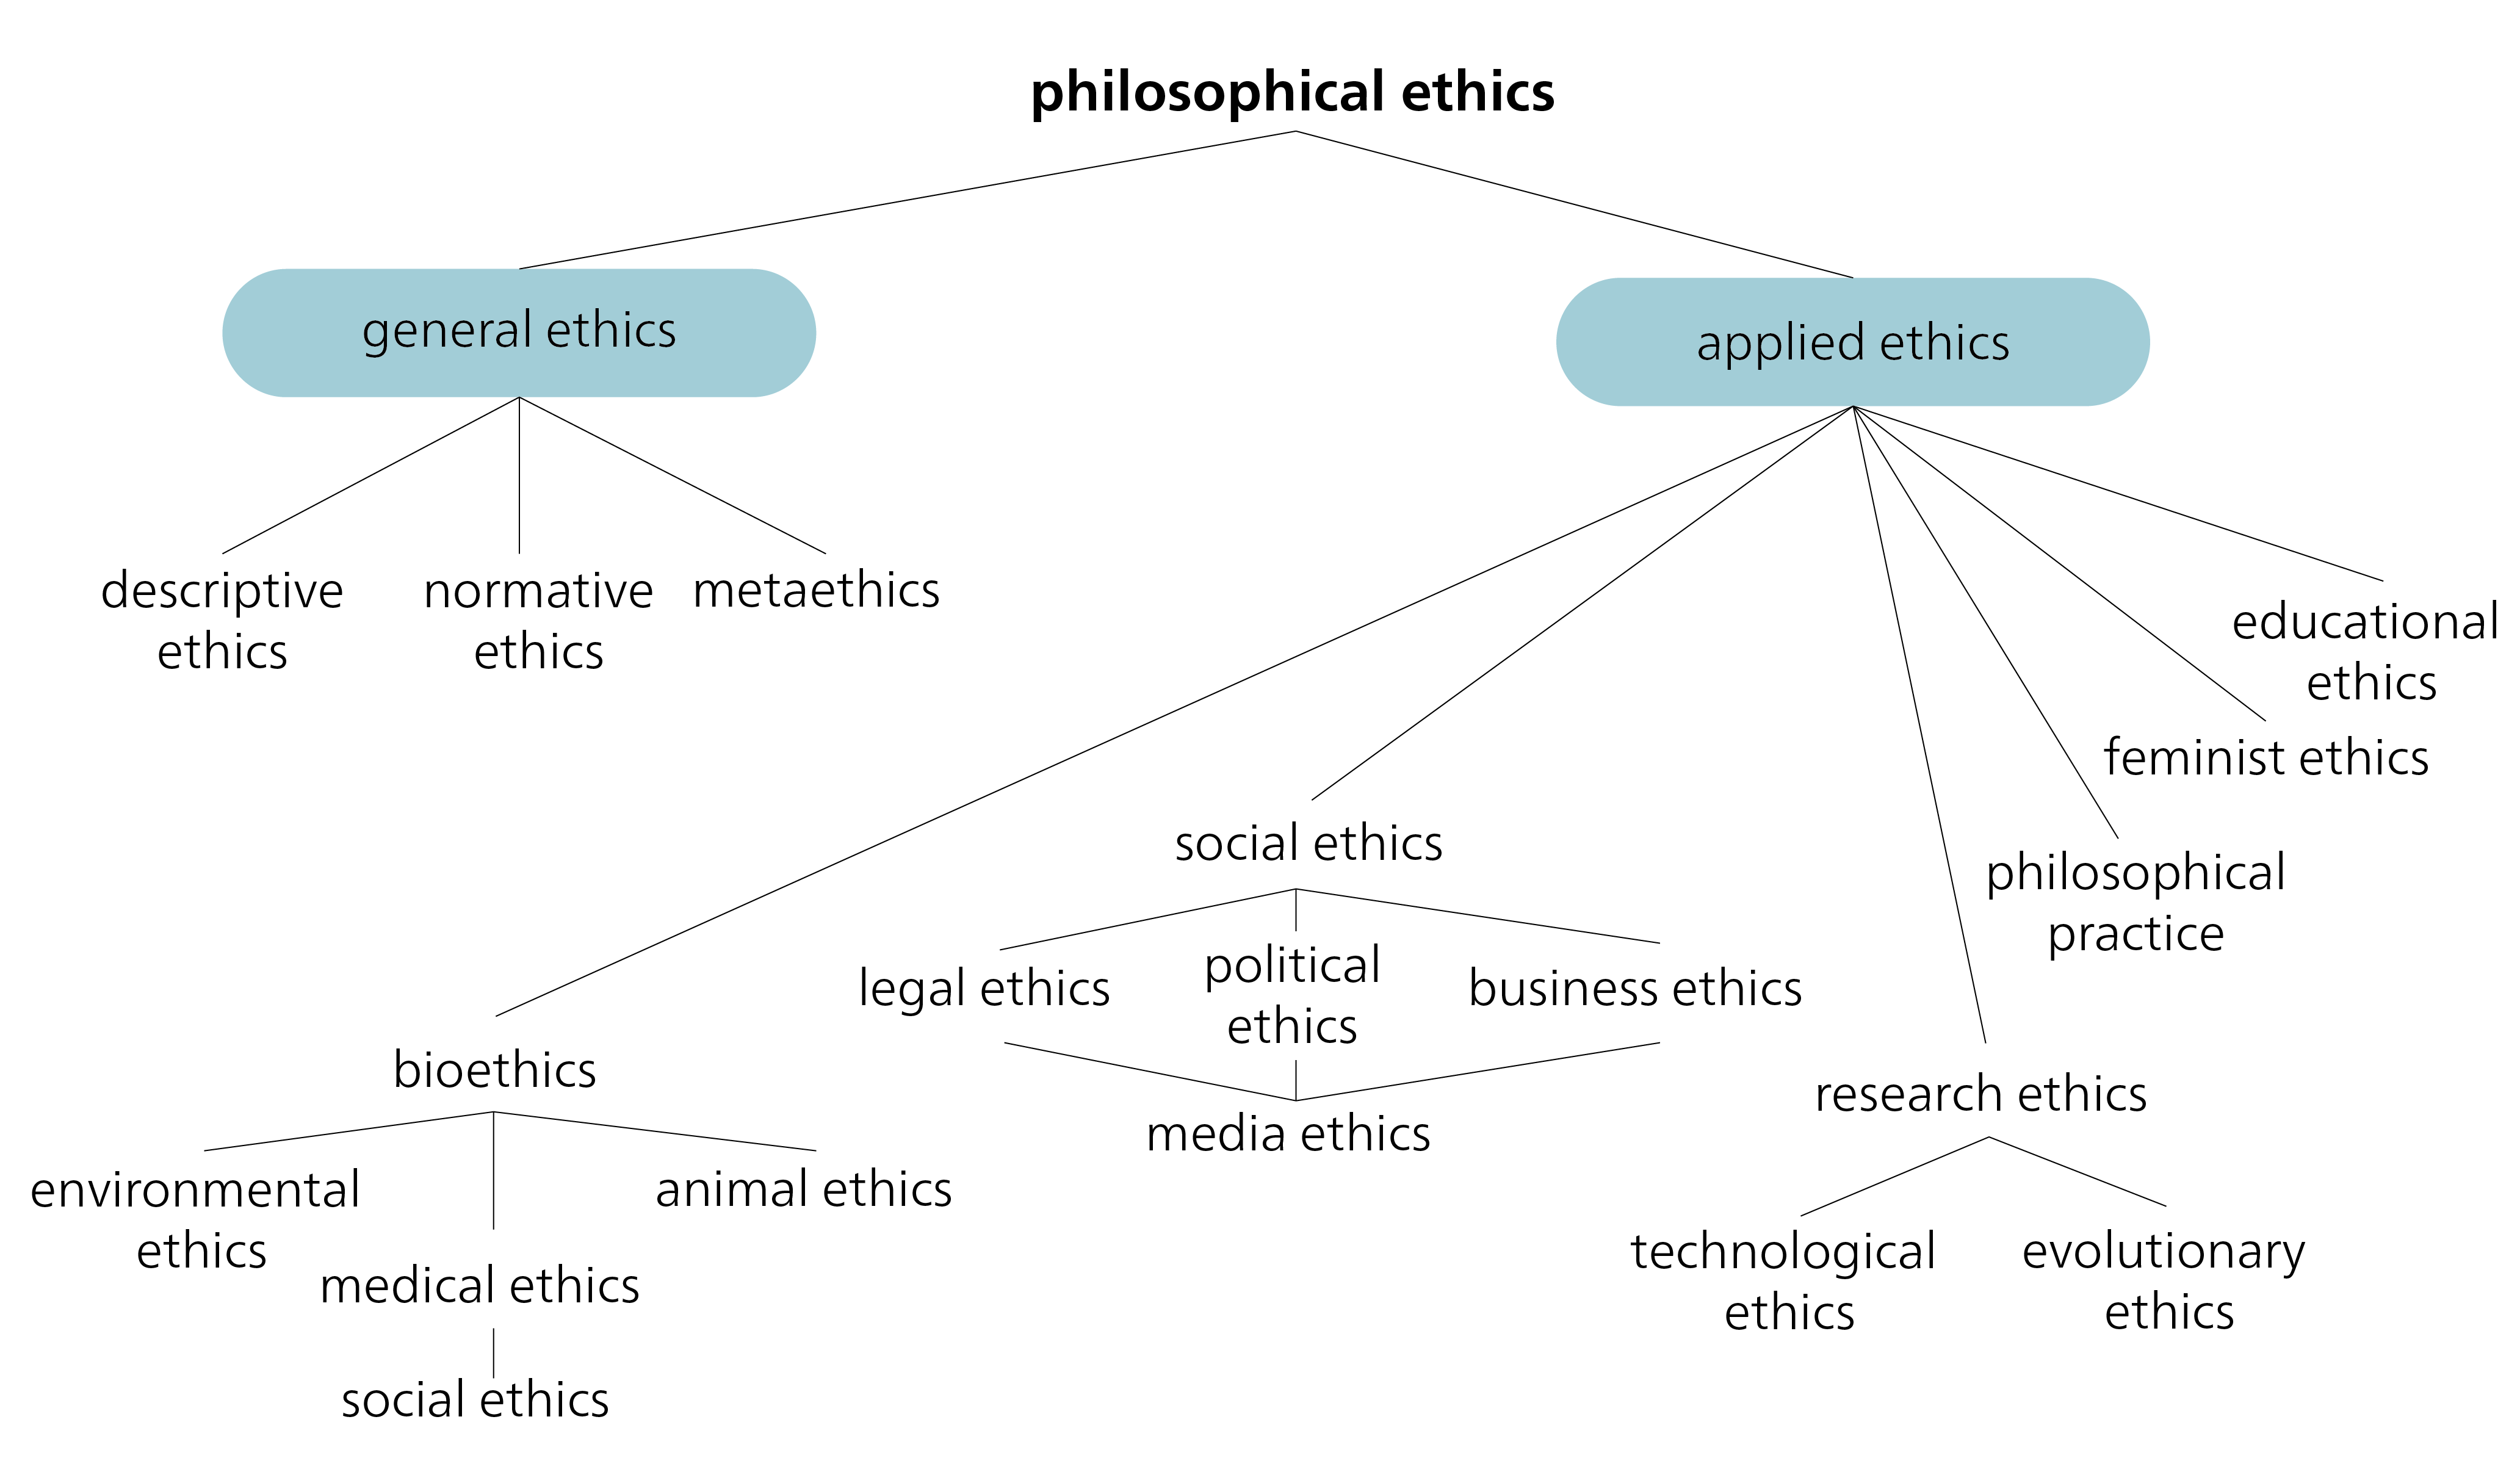
\includegraphics[keepaspectratio]{1_understanding/images/Fig1_7_EthicsBranches.png}}

}

\caption{\label{fig-branches-ethics}Die verschiedenen Zweige der
philosophischen Ethik. Quelle: Eigene Darstellung basierend auf Pieper
und Thurnherr 1998, 9.}

\end{figure}%

Die allgemeine Ethik stellt uns Methoden und Konzepte zur Verfügung, um
grundlegende moralische Probleme zu diskutieren. Sie besteht aus drei
Zweigen: normative Ethik, deskriptive Ethik und Metaethik. Die normative
Ethik konzentriert sich auf die Bestimmung dessen, was moralisch richtig
oder falsch ist. Fragen nach dem, was ein gutes Leben ausmacht, können
beispielsweise je nach den individuellen Wertvorstellungen der Menschen
unterschiedliche Antworten haben.

Aus diesem Grund wird die normative Ethik weiter in teleologische und
deontologische Ansätze unterteilt. Die teleologische Ethik (verwurzelt
in \emph{telos}, dem griechischen Wort für „Ende'', „Zweck'' oder
„Ziel'') bewertet Handlungen anhand des Guten, das sie hervorbringen.
Der Utilitarismus beispielsweise ist eine teleologische Theorie, die
Handlungen nach dem daraus resultierenden Nutzen oder Glück bewertet.
Eine der ersten systematischen Ausarbeitungen des Utilitarismus ist
Jeremy Benthams (1748--1832) \emph{An Introduction to the Principles of
Morals and Legislation} (1780). Die deontologische Ethik hingegen
bewertet Handlungen anhand ihrer Eigenschaften und nicht anhand ihrer
Konsequenzen. Ihr Ursprung liegt in \emph{deon}, dem griechischen Wort
für „Pflicht''. Ein Beispiel für eine deontologische Ethiktheorie ist
die Kantische Ethik, die vom deutschen Philosophen Immanuel Kant
entwickelt wurde.

Die Unterscheidung zwischen teleologischen und deontologischen Ansätzen
wird häufig anhand des „Trolley-Problems'' diskutiert (vgl.
\emph{Justice} 2009; Sandel 2013 für weiterführende Lektüre).

\begin{tcolorbox}[enhanced jigsaw, arc=.35mm, bottomrule=.15mm, bottomtitle=1mm, breakable, colback=white, colbacktitle=quarto-callout-caution-color!10!white, colframe=quarto-callout-caution-color-frame, coltitle=black, left=2mm, leftrule=.75mm, opacityback=0, opacitybacktitle=0.6, rightrule=.15mm, title={Weiterführende Literatur}, titlerule=0mm, toprule=.15mm, toptitle=1mm]

\begin{itemize}
\item
  \emph{Justice: What's The Right Thing To Do? Episode 01 ``THE MORAL
  SIDE OF MURDER.''} 2009. Mit Michael Sandel. The Moral Side of Murder.
  \url{https://www.youtube.com/watch?v=kBdfcR-8hEY}.
\item
  Sandel, Michael. 2013. \emph{Gerechtigkeit.} Ullstein.
\end{itemize}

\end{tcolorbox}

\subsection{Das Prinzip Verantwortung -- Hans
Jonas}\label{das-prinzip-verantwortung-hans-jonas}

Hans Jonas' „Prinzip Verantwortung'' (1979) leistet einen wichtigen
Beitrag zur Nachhaltigkeitsdebatte, indem es unsere ethische
Verantwortung gegenüber zukünftigen Generationen und der Natur betont.
Jonas' Ansatz, der als eine Art „Ethik der Zukunft'' beschrieben wurde,
zielt darauf ab, die neuen Herausforderungen zu bewältigen, die
insbesondere durch eine technologische Zivilisation entstehen. Die
Verbindung zur Nachhaltigkeitsethik liegt in seinem Verständnis des
Begriffs der ethischen Verantwortung gegenüber zukünftigen Generationen,
die er als asymmetrische, nicht-reziproke Beziehung betrachtet (Jonas
1987, pp.~177). Die Asymmetrie ergibt sich aus der Macht eines
„moralischen Subjekts'' über jemanden oder etwas, das der Fürsorge
bedarf; Jonas beschreibt die Verletzlichkeit des Lebens (ontologische
Verletzlichkeit) und die Verantwortung als unsere Sorgfaltspflicht,
andere Wesen vor Schaden zu schützen (Jonas 1987, pp.~391).

Jonas' Ansatz unterscheidet sich von anderen Ethiktheorien dadurch, dass
er die Existenz der Menschheit nicht als selbstverständlich voraussetzt
und stattdessen Pflichten gegenüber zukünftigen Generationen sowie
gegenüber der Natur einschliesst. Jonas argumentiert, dass die erste
Pflicht der Zukunftsethik darin besteht, die Fernwirkungen menschlichen
Handelns anzuerkennen (Jonas 1987, pp.~64). Angesichts der Unsicherheit
über die langfristigen Folgen menschlichen Handelns schlägt er ein
Entscheidungsprinzip vor, das auf dem lateinischen Begriff*in dubio pro
malo* basiert, den er wie folgt interpretiert: „{[}\ldots{]} gib im
Zweifel der schlimmeren Prognose vor der besseren den Vorrang, da die
Einsätze zu hoch geworden sind für das Spiel'' (Jonas 1987, pp.~67).
Jonas entwickelt damit einen neuen kategorischen Imperativ, der die
Notwendigkeit betont, sowohl die Natur als auch die Menschheit zu
erhalten. Er basiert auf der Idee, dass die Natur einen immanenten Wert
und Zweck hat: „Handle so, dass die Wirkungen deiner Handlung
verträglich sind mit der Permanenz echten menschlichen Lebens auf
Erden'', oder „Handle so, dass die Wirkungen deiner Handlung nicht
zerstörerisch sind für die künftige Möglichkeit solchen Lebens'' (Jonas
1987, pp.~36).

Bereits in den späten 1970er Jahren artikulierte Hans Jonas damit eine
grundlegende Unsicherheit über die Risiken und Schäden, die durch die
damals genutzten Technologien wie die Kernenergie für zukünftige
Generationen entstehen könnten. Entscheidungsfindung zu Themen wie neue
Technologien erfordert eine kontinuierliche Bewertung von Risiken und
Chancen, oft unter unvollständigen Informationen und unsicheren
Zukunftsprognosen. Diese Entscheidungen wirken sich nicht nur auf die
Umwelt aus, sondern werfen auch ethische Fragen über unsere
Verpflichtung auf, Nachhaltigkeit für zukünftige Generationen zu
sichern. Jonas' Verantwortungsimperativ betont die Verknüpfung von
Verantwortung und Pflicht als Schlüsselkonzepte in der
Nachhaltigkeitsdebatte. Laut Jonas tragen die gegenwärtigen Generationen
eine vorausschauende Verantwortung gegenüber zukünftigen Generationen.
Offen lässt er jedoch das Ausmass dieser Pflicht und die Frage, ob
zukünftige Generationen Anspruch auf absolute oder vergleichende
Standards haben.

Jonas' Verantwortungsimperativ kann im Zusammenhang mit verschiedenen
Verantwortungsbereichen betrachtet werden, die unterschiedliche ethische
Ansätze repräsentieren: Anthropozentrismus, Pathozentrismus,
Biozentrismus und Physiozentrismus.

\begin{figure}[H]

\centering{

\pandocbounded{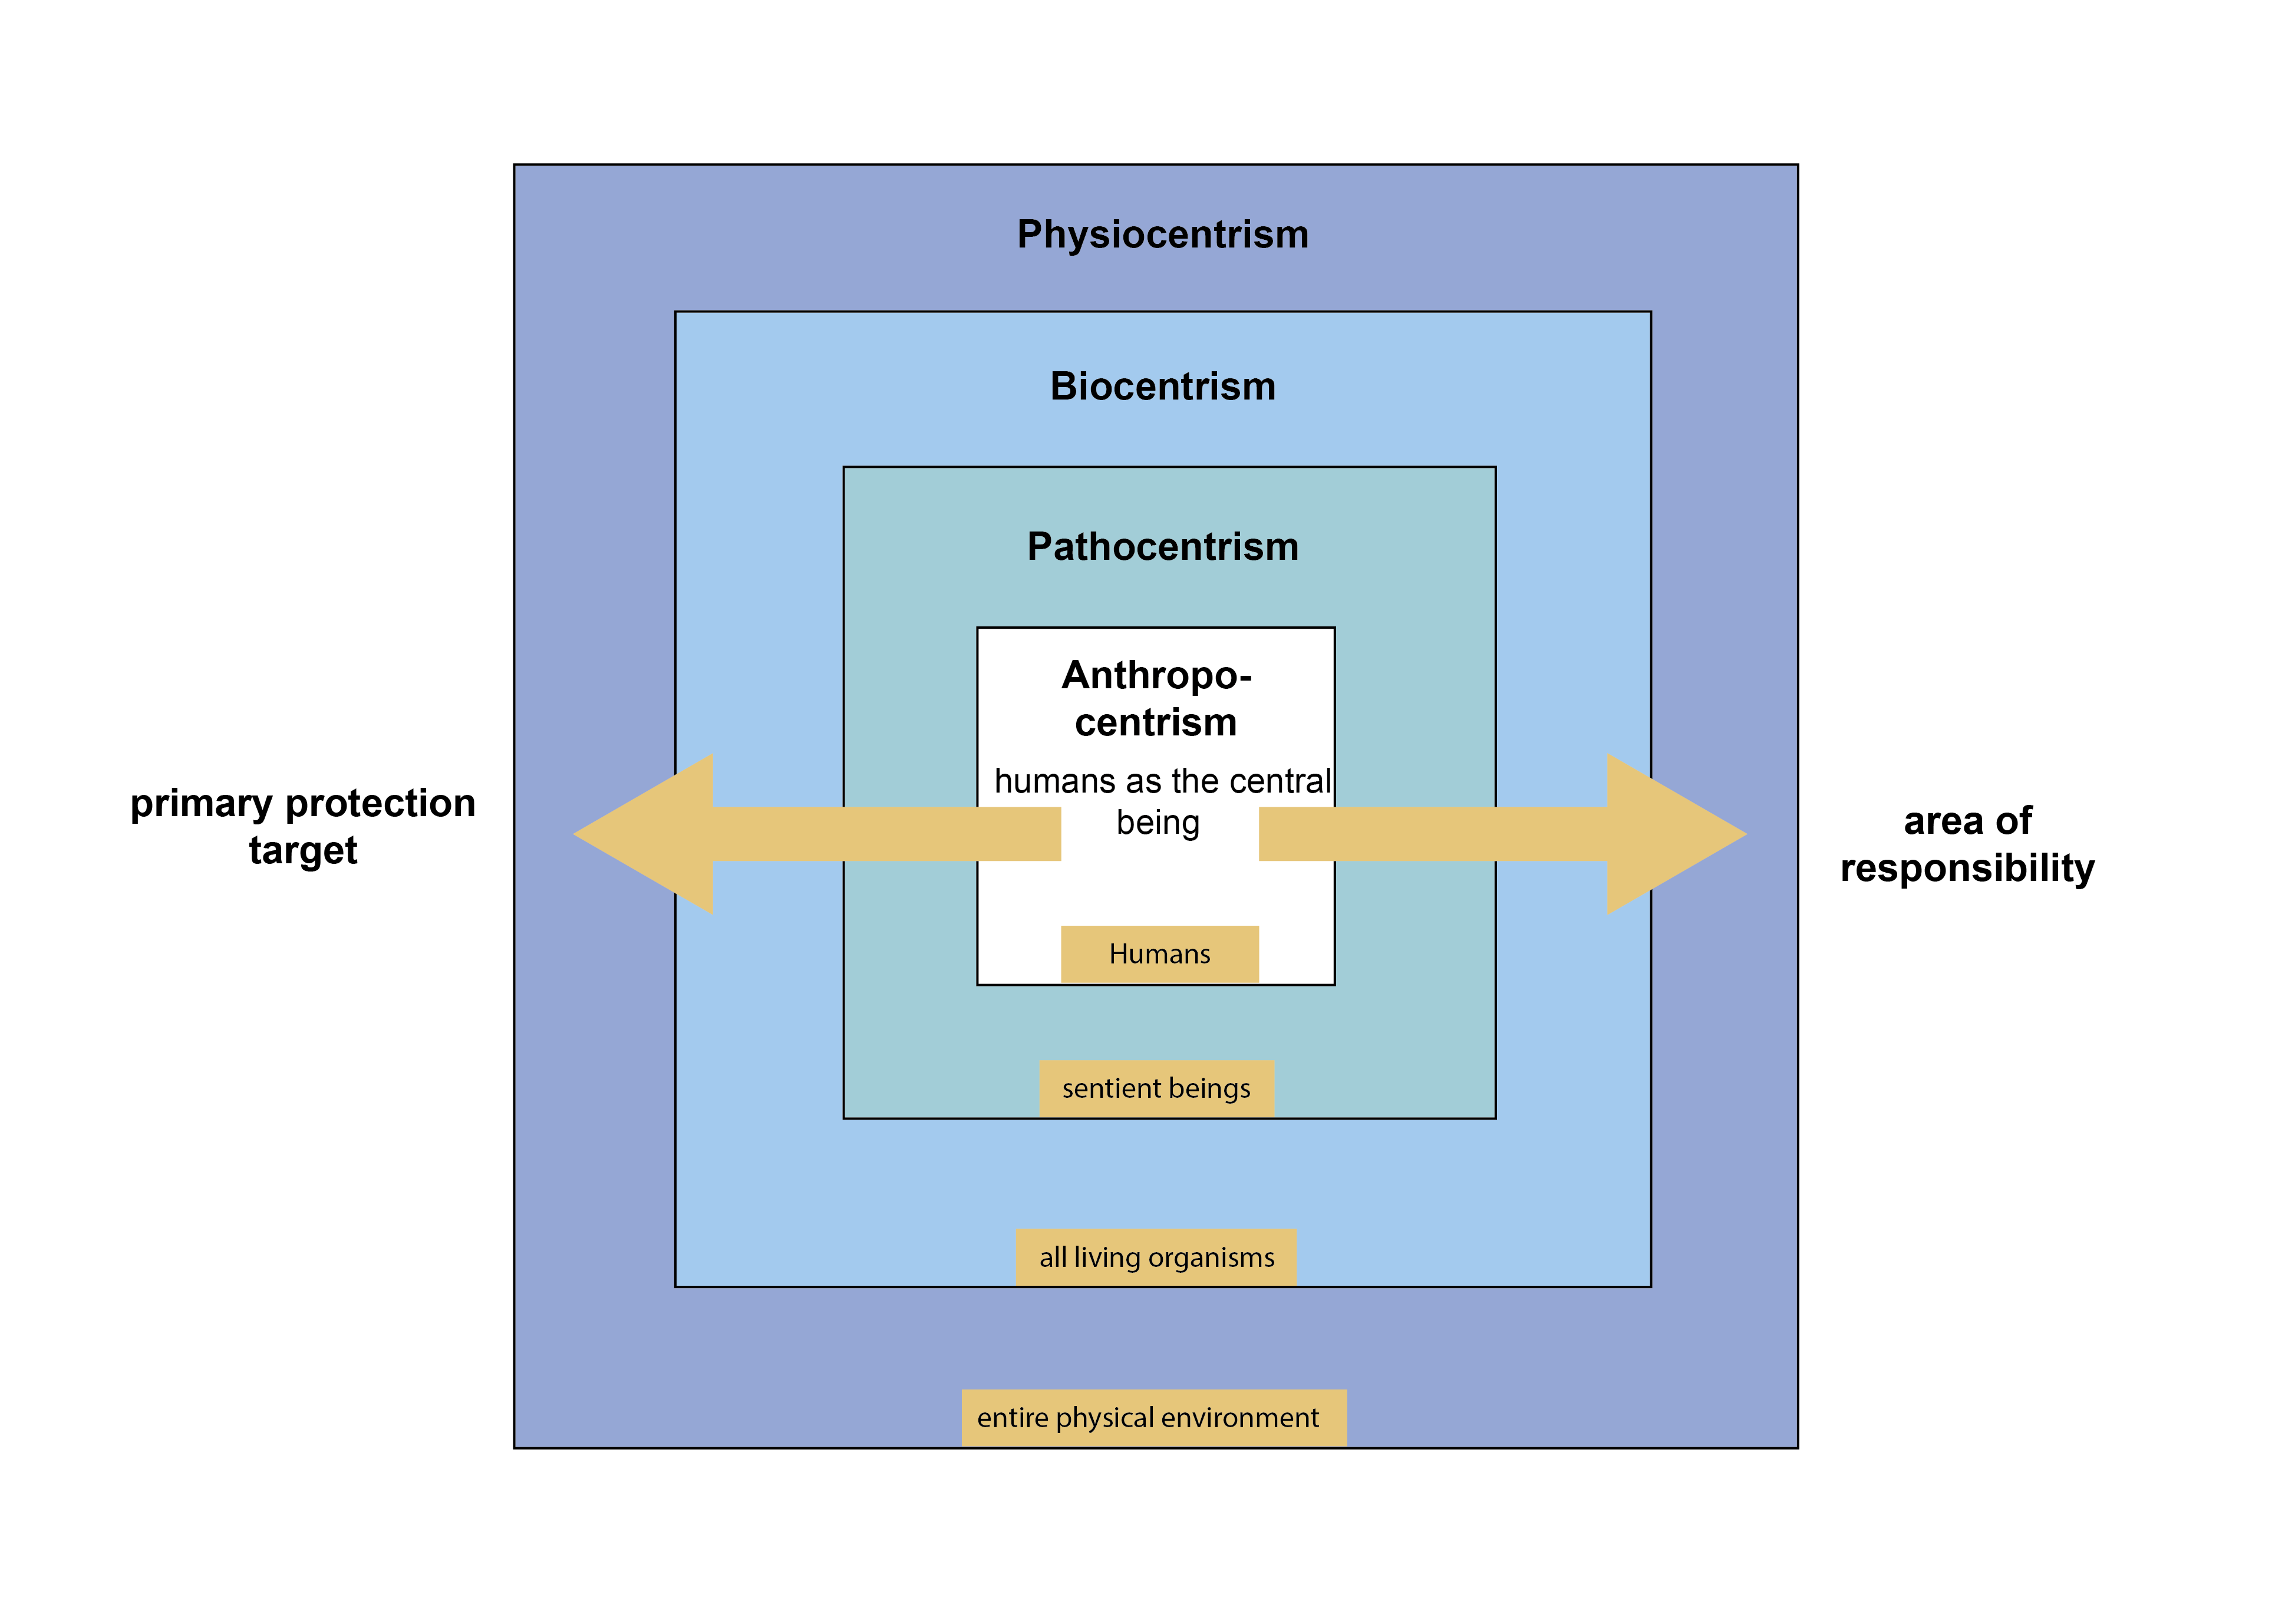
\includegraphics[keepaspectratio]{1_understanding/images/Anthropocentrism-13.png}}

}

\caption{\label{fig-anthropocentrism}Verschiedene ethische Ansätze.
Quelle: Eigene Darstellung basierend auf Carnau (2011, p.~143).}

\end{figure}%

Der Anthropozentrismus betrachtet den Menschen als das zentrale Wesen
und betont die Verantwortung gegenüber der menschlichen Gesellschaft und
ihrem Wohlergehen. Dies schliesst die Berücksichtigung der Bedürfnisse
und Interessen sowohl der gegenwärtigen als auch der zukünftigen
Generationen ein. Der Pathozentrismus hingegen betont die Verantwortung
gegenüber empfindungsfähigen Wesen und ihrem Wohlbefinden. Er erkennt
an, dass nicht nur Menschen, sondern auch Tiere und andere Lebewesen das
Recht haben, frei von Leid und Schaden zu sein. Der Biozentrismus
wiederum erkennt den immanenten Wert aller Lebewesen an und konzentriert
sich auf den Schutz und die Erhaltung der Biodiversität. Er betont die
Bedeutung der Achtung der natürlichen Umwelt und die Förderung
nachhaltiger Praktiken. Schliesslich konzentriert sich der
Physiozentrismus auf die Verantwortung gegenüber der gesamten physischen
Umwelt, einschliesslich der unbelebten Natur und der Ökosysteme. Er
erkennt den immanenten Wert der Natur an und betont die komplexen
Wechselwirkungen zwischen allen Komponenten des Ökosystems.

Hans Jonas' Verantwortungsimperativ verbindet alle diese verschiedenen
Verantwortungsbereiche miteinander. Er fordert uns auf, Verantwortung
für Menschen sowie für andere Lebewesen, die Natur und die Umwelt zu
übernehmen. Dabei ist es wichtig, eine ausgewogene und umfassende
Perspektive einzunehmen, die langfristige Auswirkungen und das
Wohlbefinden aller Aspekte des Lebens und der Natur berücksichtigt.

Durch die Integration dieser verschiedenen Verantwortungsbereiche können
wir eine ganzheitliche und nachhaltige Ethik kultivieren, die den
Bedürfnissen und Interessen aller Aspekte des Lebens und der Natur
angemessen Rechnung trägt.

\section{Nachhaltige Entwicklung im Kontext von
Entwicklungsdebatten}\label{nachhaltige-entwicklung-im-kontext-von-entwicklungsdebatten}

Ist „Nachhaltige Entwicklung'' eine Entwicklungstheorie? Jein. Nein,
weil Nachhaltige Entwicklung ein breiteres gesellschaftliches Modell ist
und als übergreifender Rahmen fungiert, der verschiedene
Entwicklungstheorien umfasst. Ja, weil Nachhaltige Entwicklung eine
normative Theorie ist, die de facto in der wissenschaftlichen und
gesellschaftlichen Praxis mit anderen Theorien der sozialen und
insbesondere sozioökonomischen Entwicklung konkurriert.

Entwicklungstheorien analysieren die gesellschaftliche Entwicklung,
entweder retrospektiv oder prospektiv, und entweder als Ganzes oder
anhand spezifischer Aspekte (z. B. wirtschaftliche Entwicklung). Die
retrospektive Untersuchung der gesellschaftlichen Entwicklung zielt
darauf ab, vergangene oder aktuelle gesellschaftliche Entwicklungen zu
erklären und Lehren für die künftige Planung und Entwicklungspolitik zu
ziehen. Die prospektive Untersuchung der gesellschaftlichen Entwicklung
soll das Management und die Politik der gesellschaftlichen Entwicklung
informieren. Entwicklungstheorien können in verschiedene Typen
eingeteilt werden: normative, strategische und erklärende Theorien.
Jeder Typ konzentriert sich auf unterschiedliche Aspekte und Ziele der
Entwicklungsforschung.

Normative Theorien konzentrieren sich auf die Frage, wie Entwicklung
aussehen sollte und welche normativen Ziele sie erreichen sollte. Sie
untersuchen Werte und Ziele, die mit Entwicklung verbunden sind, und
beziehen sich häufig auf Konzepte wie soziale Gerechtigkeit,
Nachhaltigkeit oder Armutsbekämpfung. Normative Theorien betonen die
Definition von Kriterien für gute Entwicklung und liefern einen
normativen Rahmen für politische Entscheidungen und Massnahmen.
Beispiele sind die Theorie der Nachhaltigen Entwicklung, John Rawls'
Theorie der sozialen Gerechtigkeit oder Amartya Sens Capability-Ansatz.

Strategische Theorien untersuchen, welche Strategien und Massnahmen
erforderlich sind, um gewünschte Entwicklungsergebnisse zu erzielen. Sie
konzentrieren sich auf Fragen der Politikgestaltung, der
Ressourcenallokation und der Umsetzung von Massnahmen und analysieren,
wie bestimmte Ansätze -- etwa die neoklassische Wachstumstheorie -- die
Entwicklung fördern können.

Erklärende Theorien zielen darauf ab, die Ursachen und Mechanismen von
Entwicklung zu erklären. Sie analysieren Faktoren, die
Entwicklungsprozesse in Gesellschaften antreiben, und untersuchen die
Zusammenhänge zwischen den verschiedenen Variablen. Dies umfasst die
Untersuchung wirtschaftlicher, sozialer, politischer oder kultureller
Faktoren, um Muster und Zusammenhänge zu identifizieren. Beispiele sind
die Modernisierungstheorie und die Dependenztheorie.

Hinweis: Alle Theorien beruhen auf normativen Grundlagen -- d.~h. auf
zugrunde liegenden Werten und Überzeugungen -- und implizieren daher,
auch unbeabsichtigt, bestimmte Vorstellungen davon, wie sich die
Gesellschaft entwickeln sollte.

\begingroup\fontsize{8}{10}\selectfont

\begin{longtable}[t]{>{\raggedright\arraybackslash}p{1.6cm}>{\raggedright\arraybackslash}p{2.3cm}>{\raggedright\arraybackslash}p{2.3cm}>{\raggedright\arraybackslash}p{2.3cm}>{\raggedright\arraybackslash}p{2.3cm}>{\raggedright\arraybackslash}p{2.3cm}}

\caption{\label{tbl-development-theories}Überblick über
Entwicklungsdebatten. Quelle: Erweiterte Tabelle basierend auf Bieri
(2022, 378).}

\tabularnewline

\toprule
\textbf{Kategorie} & \textbf{1950er/60er Jahre} & \textbf{1970er Jahre} & \textbf{1980er Jahre} & \textbf{1990er Jahre} & \textbf{Seit 2008}\\
\midrule
\endfirsthead
\multicolumn{6}{@{}l}{\textit{(continued)}}\\
\toprule
\textbf{Kategorie} & \textbf{1950er/60er Jahre} & \textbf{1970er Jahre} & \textbf{1980er Jahre} & \textbf{1990er Jahre} & \textbf{Seit 2008}\\
\midrule
\endhead

\endfoot
\bottomrule
\endlastfoot
\textbf{Narrativ} & Wirtschaftswachstum, Modernisierung und Integration in die Weltwirtschaft & Bekämpfung extremer Armut und Ungleichheit & Verlorenes Jahrzehnt: Zusammenbruch der Rohstoffpreise; Zunahme der Verschuldung & Nachhaltige Entwicklung; Jahrzehnt der Hoffnung & Polykrise\\
\textbf{Grundidee} & Aufholentwicklung durch Industrialisierung und Grossprojekte & Befriedigung der Grundbedürfnisse, Wachstum und effektive Verteilung & Überwindung der Schuldenkrise durch Strukturanpassungsmassnahmen, Abbau staatlicher Leistungen & Globale und nachhaltige Umweltpolitik, Wirtschaftswachstum, Friedenssicherung, Fortführung der Grundbedürfnisstrategie, Partizipation & Zusammenführen verschiedener Krisenphänomene (Finanzkrise, Klimawandel, Biodiversitätskrise usw.) und Untersuchung ihrer komplexen Wechselwirkungen; Suche nach integrierten Lösungen\\
\textbf{Theorien} & Modernisierungs­theorien (Stufentheorien) & Dependenztheorien versus Modernisierungs­theorien & Marktliberalismus und Neoliberalismus & Theorien der Nachhaltigen Entwicklung, Neoklassische Wachstumstheorie, Postkoloniale Theorien, Capability-Ansatz, Postentwicklungstheorien & Zusätzlich Resilienztheorien, Postwachstumstheorien\\
\textbf{Ziele} & Geopolitische Einordnung der „Dritten Welt“; Eindämmung des Kommunismus, Modernisierung der Landwirtschaft, rasche Industrialisierung und technologischer Fortschritt, Erschliessung neuer Märkte & Hilfe zur Selbsthilfe, angepasste Technologien, ländliche Entwicklung, Frauenförderung & Steigerung der Exporte, ausgeglichene Staatshaushalte & Paradigmenwechsel in der Entwicklungshilfe hin zur Entwicklungszusammenarbeit, ökologische und soziale Verträglichkeit von Entwicklung, Sicherstellung des Zugangs zu Ressourcen und Infrastruktur für alle & \\
\textbf{Folgen} & Wirtschaftliche Abhängigkeit und Verschuldung nehmen zu, Einkommensgefälle wächst, Armut steigt, ökologische Schäden durch Übernutzung und unangepasste Technologien, undemokratische Regime werden aus geopolitischen Gründen unterstützt & Selektive Fortschritte in Bildung und Gesundheit, Probleme mit Verschuldung und Umweltschäden & Lebensstandard der ärmsten Bevölkerungsgruppen verschlechtert sich stark, Umweltausbeutung, Schuldenspirale, zunehmende Abhängigkeit des Globalen Südens vom Globalen Norden & Der Fokus verlagert sich von rein wirtschaftlicher Entwicklung auf menschliche Entwicklung; Industrieländer sind zur Umsetzung Nachhaltiger Entwicklung verpflichtet; Entstehung einer globalen Entwicklungspartnerschaft & \\*

\end{longtable}

\endgroup{}

\begin{tcolorbox}[enhanced jigsaw, arc=.35mm, bottomrule=.15mm, bottomtitle=1mm, breakable, colback=white, colbacktitle=quarto-callout-note-color!10!white, colframe=quarto-callout-note-color-frame, coltitle=black, left=2mm, leftrule=.75mm, opacityback=0, opacitybacktitle=0.6, rightrule=.15mm, title={Entwicklungstheorien}, titlerule=0mm, toprule=.15mm, toptitle=1mm]

\textbf{Modernisierungstheorie} (1950er--1980er Jahre) betont den
Übergang von traditionellen zu modernen, industrialisierten
Gesellschaften als Grundlage für Entwicklung. Für Befürworter*innen der
Modernisierungstheorie entwickeln sich die Länder des Globalen Südens in
dieselbe Richtung wie die Industrieländer, allerdings in einem viel
langsameren Tempo. Die Modernisierungstheorie bewertet
Wirtschaftswachstum, technologischen Fortschritt und institutionelle
Anpassungen. Sie wird häufig mit Stufentheorien assoziiert, die in den
1950er und 1960er Jahren entstanden. Stufentheorien betrachten
Entwicklung als einen schrittweisen Prozess, der durch klar definierte
Stufen oder Phasen der Entwicklung gekennzeichnet ist, mit Betonung von
Wirtschaftswachstum und Modernisierung. Zu den prominenten
Vertreter*innen gehört Walt Rostow, der in seinem Werk \emph{The Stages
of Economic Growth: A Non-Communist Manifesto} fünf Entwicklungsstufen
identifizierte (d.~h. traditionelle Gesellschaft, Voraussetzungen für
den Abflug, Abflug, Reife, Massenkonsum).

\textbf{Dependenztheorie} (1970er und 1980er Jahre) betont die
strukturelle Abhängigkeit und Ungleichheit zwischen entwickelten und
sich entwickelnden Ländern. Sie argumentiert, dass Entwicklungsländer in
einem ungerechten globalen Wirtschaftssystem gefangen und von den
entwickelten Ländern abhängig bleiben.

\textbf{Neoklassische Wachstumstheorie} (ab den 1990er Jahren)
konzentriert sich auf den Zusammenhang zwischen Kapitalakkumulation,
technologischem Fortschritt und Wirtschaftswachstum. Sie betont freie
Märkte, Handel und Investitionen als Triebkräfte der Entwicklung.

\textbf{Postkoloniale Theorien} (ab den 1990er Jahren) betonen die
historische und strukturelle Ungleichheit zwischen ehemaligen
Kolonialmächten und Kolonien. Sie argumentieren, dass Entwicklung nur
durch eine kritische Auseinandersetzung mit dem Erbe des Kolonialismus
erreicht werden kann.

\textbf{Sens Capability-Ansatz} (ab den 1990er Jahren) betont die
Bedeutung von Freiheit, sozialer Gerechtigkeit und menschlicher
Entwicklung. Er unterstreicht die Notwendigkeit, die Möglichkeiten und
Fähigkeiten der Menschen zu verbessern, um Entwicklung zu erreichen.

\textbf{Postentwicklungstheorien} (ab den 1990er Jahren) kritisieren
lineare Entwicklungsmodelle, die westliche Fortschrittsvorstellungen
aufzwingen, und betonen stattdessen lokale Praktiken und Werte. Zu den
prominenten Denker*innen in diesem Bereich gehört Arturo Escobar, der
die Idee der Entwicklung in seinem Werk \emph{Encountering Development:
The Making and Unmaking of the Third World} kritisch reflektiert, sowie
Vandana Shiva, deren \emph{Decolonizing the North} eine nachhaltige und
gerechtere Entwicklungspolitik im Globalen Süden fordert, die den
Einfluss des Globalen Nordens reduziert.

\end{tcolorbox}

\section{Nachhaltigkeitsmodelle}\label{nachhaltigkeitsmodelle}

\subsection{Drei Dimensionen der
Nachhaltigkeit}\label{drei-dimensionen-der-nachhaltigkeit}

Das etablierte Drei-Säulen-Modell der Nachhaltigkeit, das im
Brundtland-Bericht von 1987 eingeführt wurde, strebt nach einem
Gleichgewicht zwischen ökologischen, wirtschaftlichen und sozialen
Belangen. Dieses Modell, das später auch als „Triple Bottom
Line''-Modell bekannt wurde, betonte, dass wirtschaftliche Entwicklung
profitabel sein sollte und gleichzeitig sicherstellt, dass die
ökologischen und sozialen Auswirkungen neutral bleiben. Bei näherer
Betrachtung weist das Modell -- anfangs als Gebäude mit drei Säulen
dargestellt -- jedoch eine wesentliche Schwäche auf. Während es
suggerieren sollte, dass das System insgesamt nicht nachhaltig wäre,
wenn eine Säule schwach ist, könnte man argumentieren, dass das
Entfernen einer der Säulen -- oder sogar der beiden äusseren Säulen --
das Gebäude nicht zum Einsturz bringen würde, wenn die verbleibende(n)
Säule(n) stark genug wären. Trotz seiner weiten Verbreitung und seines
allgemeinen Erfolgs kämpft das Modell mit Transparenz- und
Gerechtigkeitsproblemen. Zur Messung des wirtschaftlichen Erfolgs sind
beispielsweise quantitative Indikatoren erforderlich, während es schwer
ist, ähnliche Metriken für das soziale Wohlbefinden, insbesondere
emotionale Aspekte, zu finden. Einige Kritiker*innen argumentieren, dass
das Modell konventionelles wirtschaftliches Denken priorisiert und
wichtige soziale Aspekte vernachlässigt. Eine übermässige Betonung
menschlicher Wirtschaftssysteme kann uns auch daran hindern, unsere
Abhängigkeit von nicht-menschlichen ökologischen Systemen zu erkennen.

\subsection{Nachhaltigkeit als
Schnittmenge}\label{nachhaltigkeit-als-schnittmenge}

\begin{figure}[H]

\centering{

\pandocbounded{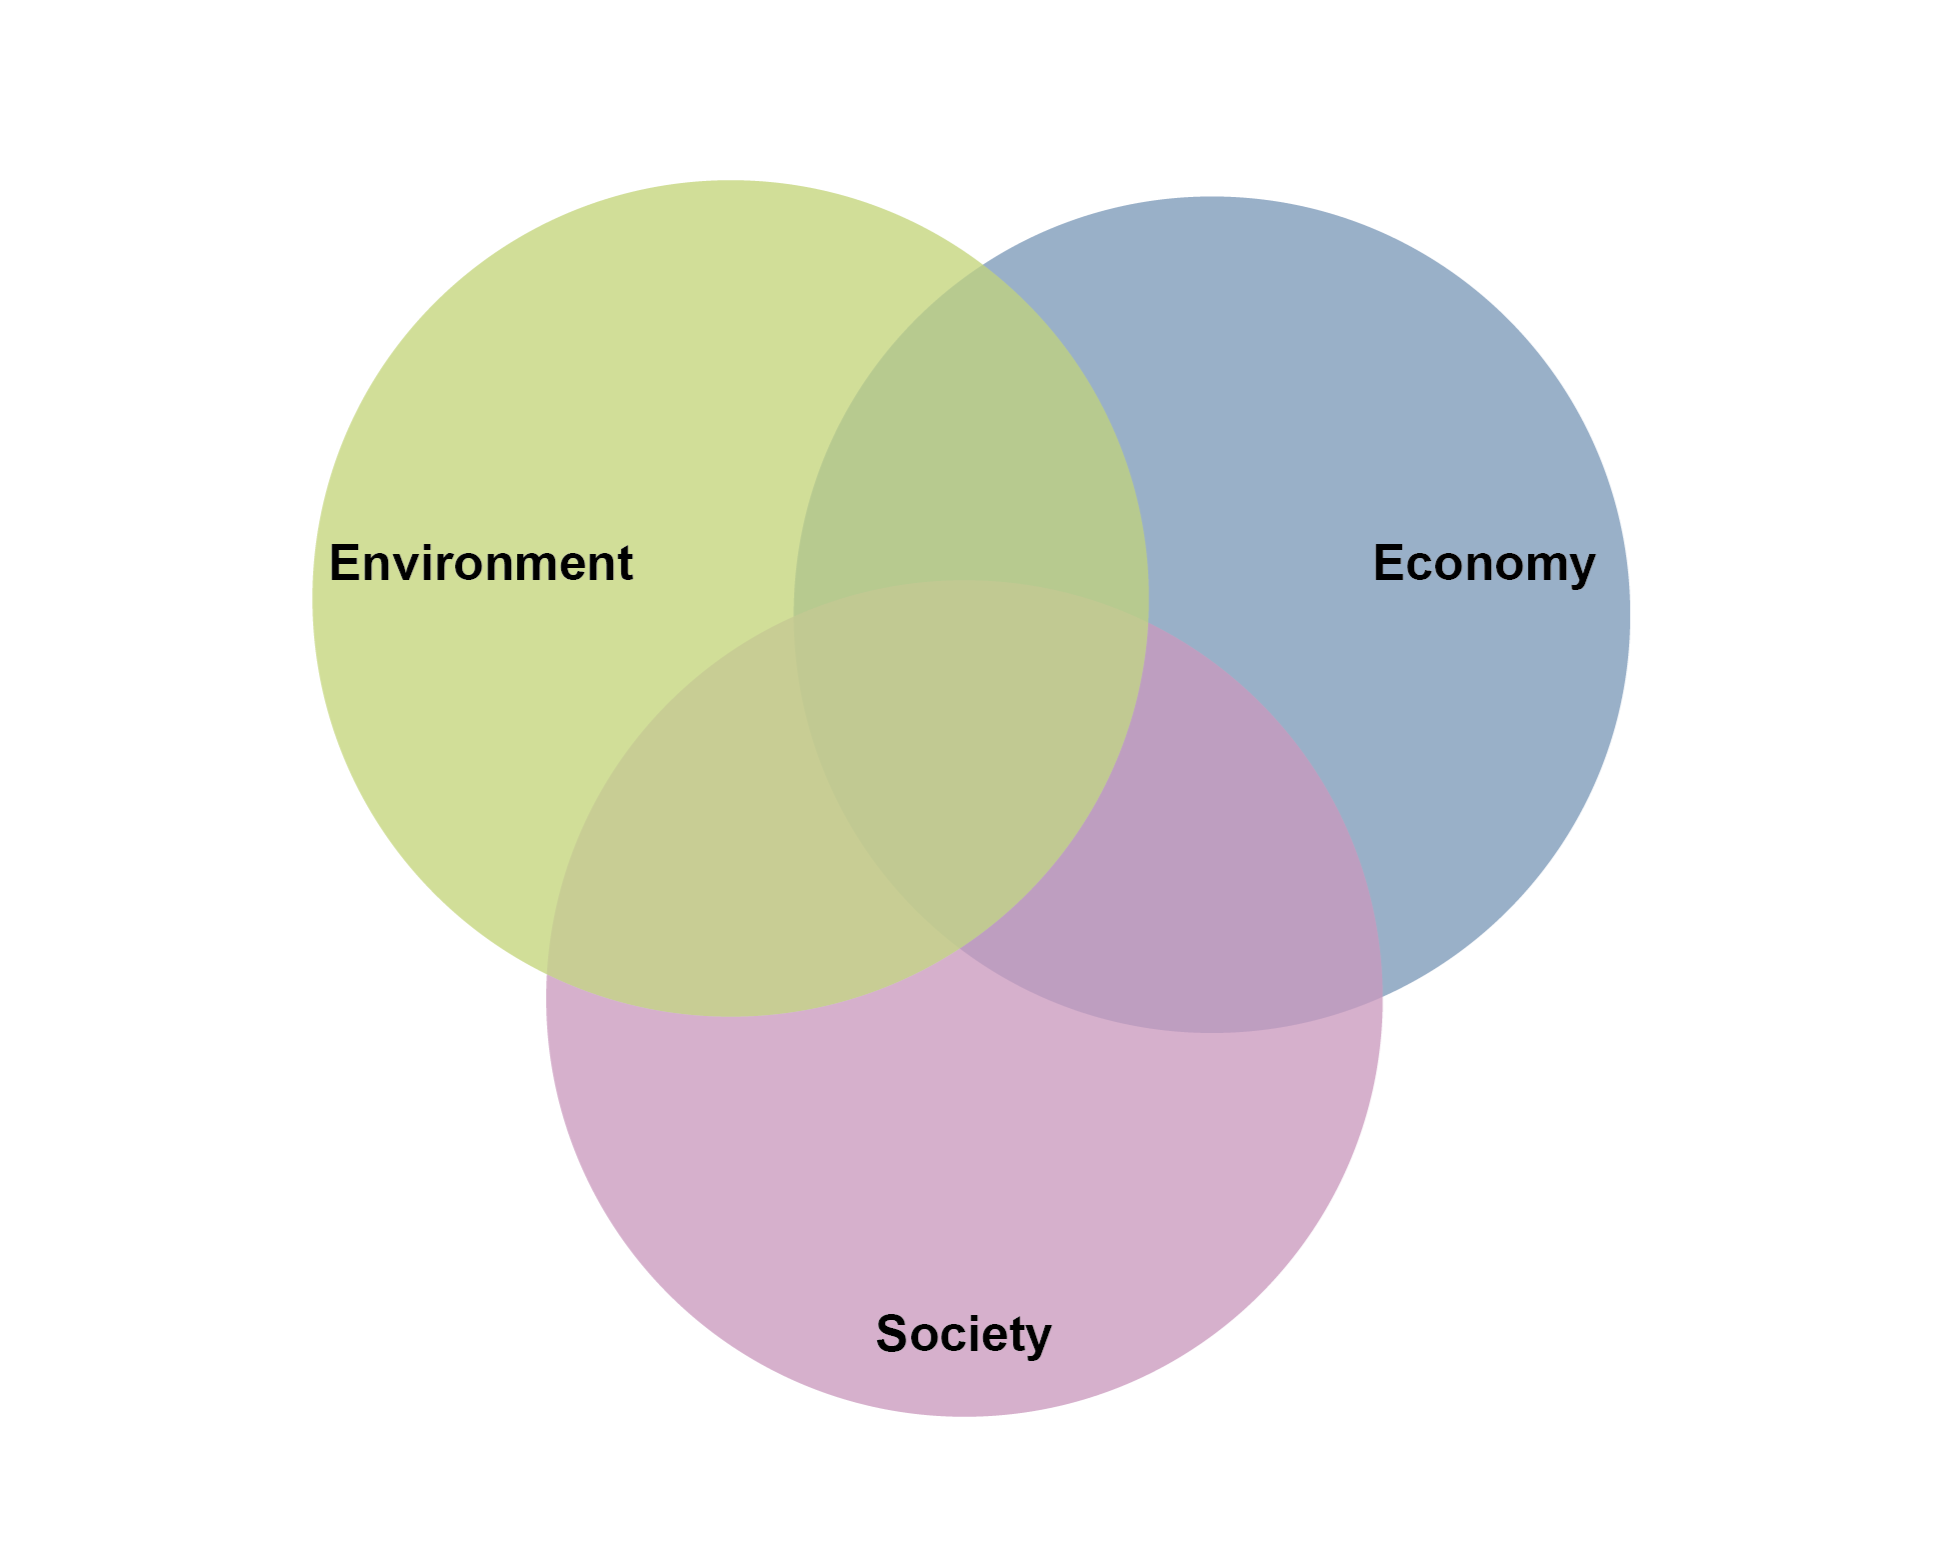
\includegraphics[keepaspectratio]{1_understanding/images/sustainability-intersection.png}}

}

\caption{\label{fig-sustainability-intersection}Nachhaltigkeit als
Schnittmenge. Quelle: Eigene Darstellung.}

\end{figure}%

Ein Modell, das die drei Sektoren als Venn-Diagramm (überlappende Ringe
oder Kreise, manchmal auch als Schnittmengen- oder Triadenmodell
bezeichnet) darstellt, bietet eine Alternative zu den separaten Säulen
und betont die Verflechtung der drei Dimensionen. Dieses Modell
veranschaulicht, dass zwischen zwei Bereichen eine engere Verbindung
bestehen kann und dass die Grenzen fliessend sind.

\subsection{Verschachtelte Nachhaltige
Entwicklung}\label{verschachtelte-nachhaltige-entwicklung}

Giddings u.~a. (2002) stellen die Idee separater Sphären für Wirtschaft,
Gesellschaft und Umwelt in Frage. Sie schlagen ein „verschachteltes''
Modell vor, bei dem die Wirtschaft als Teil der Gesellschaft betrachtet
wird, die wiederum in die Umwelt eingebettet ist. Dieses Modell, so ihre
Argumentation, stellt sicher, dass wirtschaftliche Entscheidungen stets
durch soziale und ökologische Faktoren begrenzt werden. Globale
Ökosysteme bilden die Grundlage für soziale Systeme (d.~h. die
Gesellschaft). Darin eingebettet ist die Wirtschaft, die den
Bedürfnissen der Gesellschaft dient. Ein potenzieller Nachteil dieses
Modells besteht jedoch darin, dass die Wirtschaft, wenn sie der
Ausgangspunkt aller Nachhaltigkeitsüberlegungen ist, Gefahr läuft,
gegenüber sozialen und ökologischen Überlegungen priorisiert zu werden.

\begin{figure}[H]

\centering{

\pandocbounded{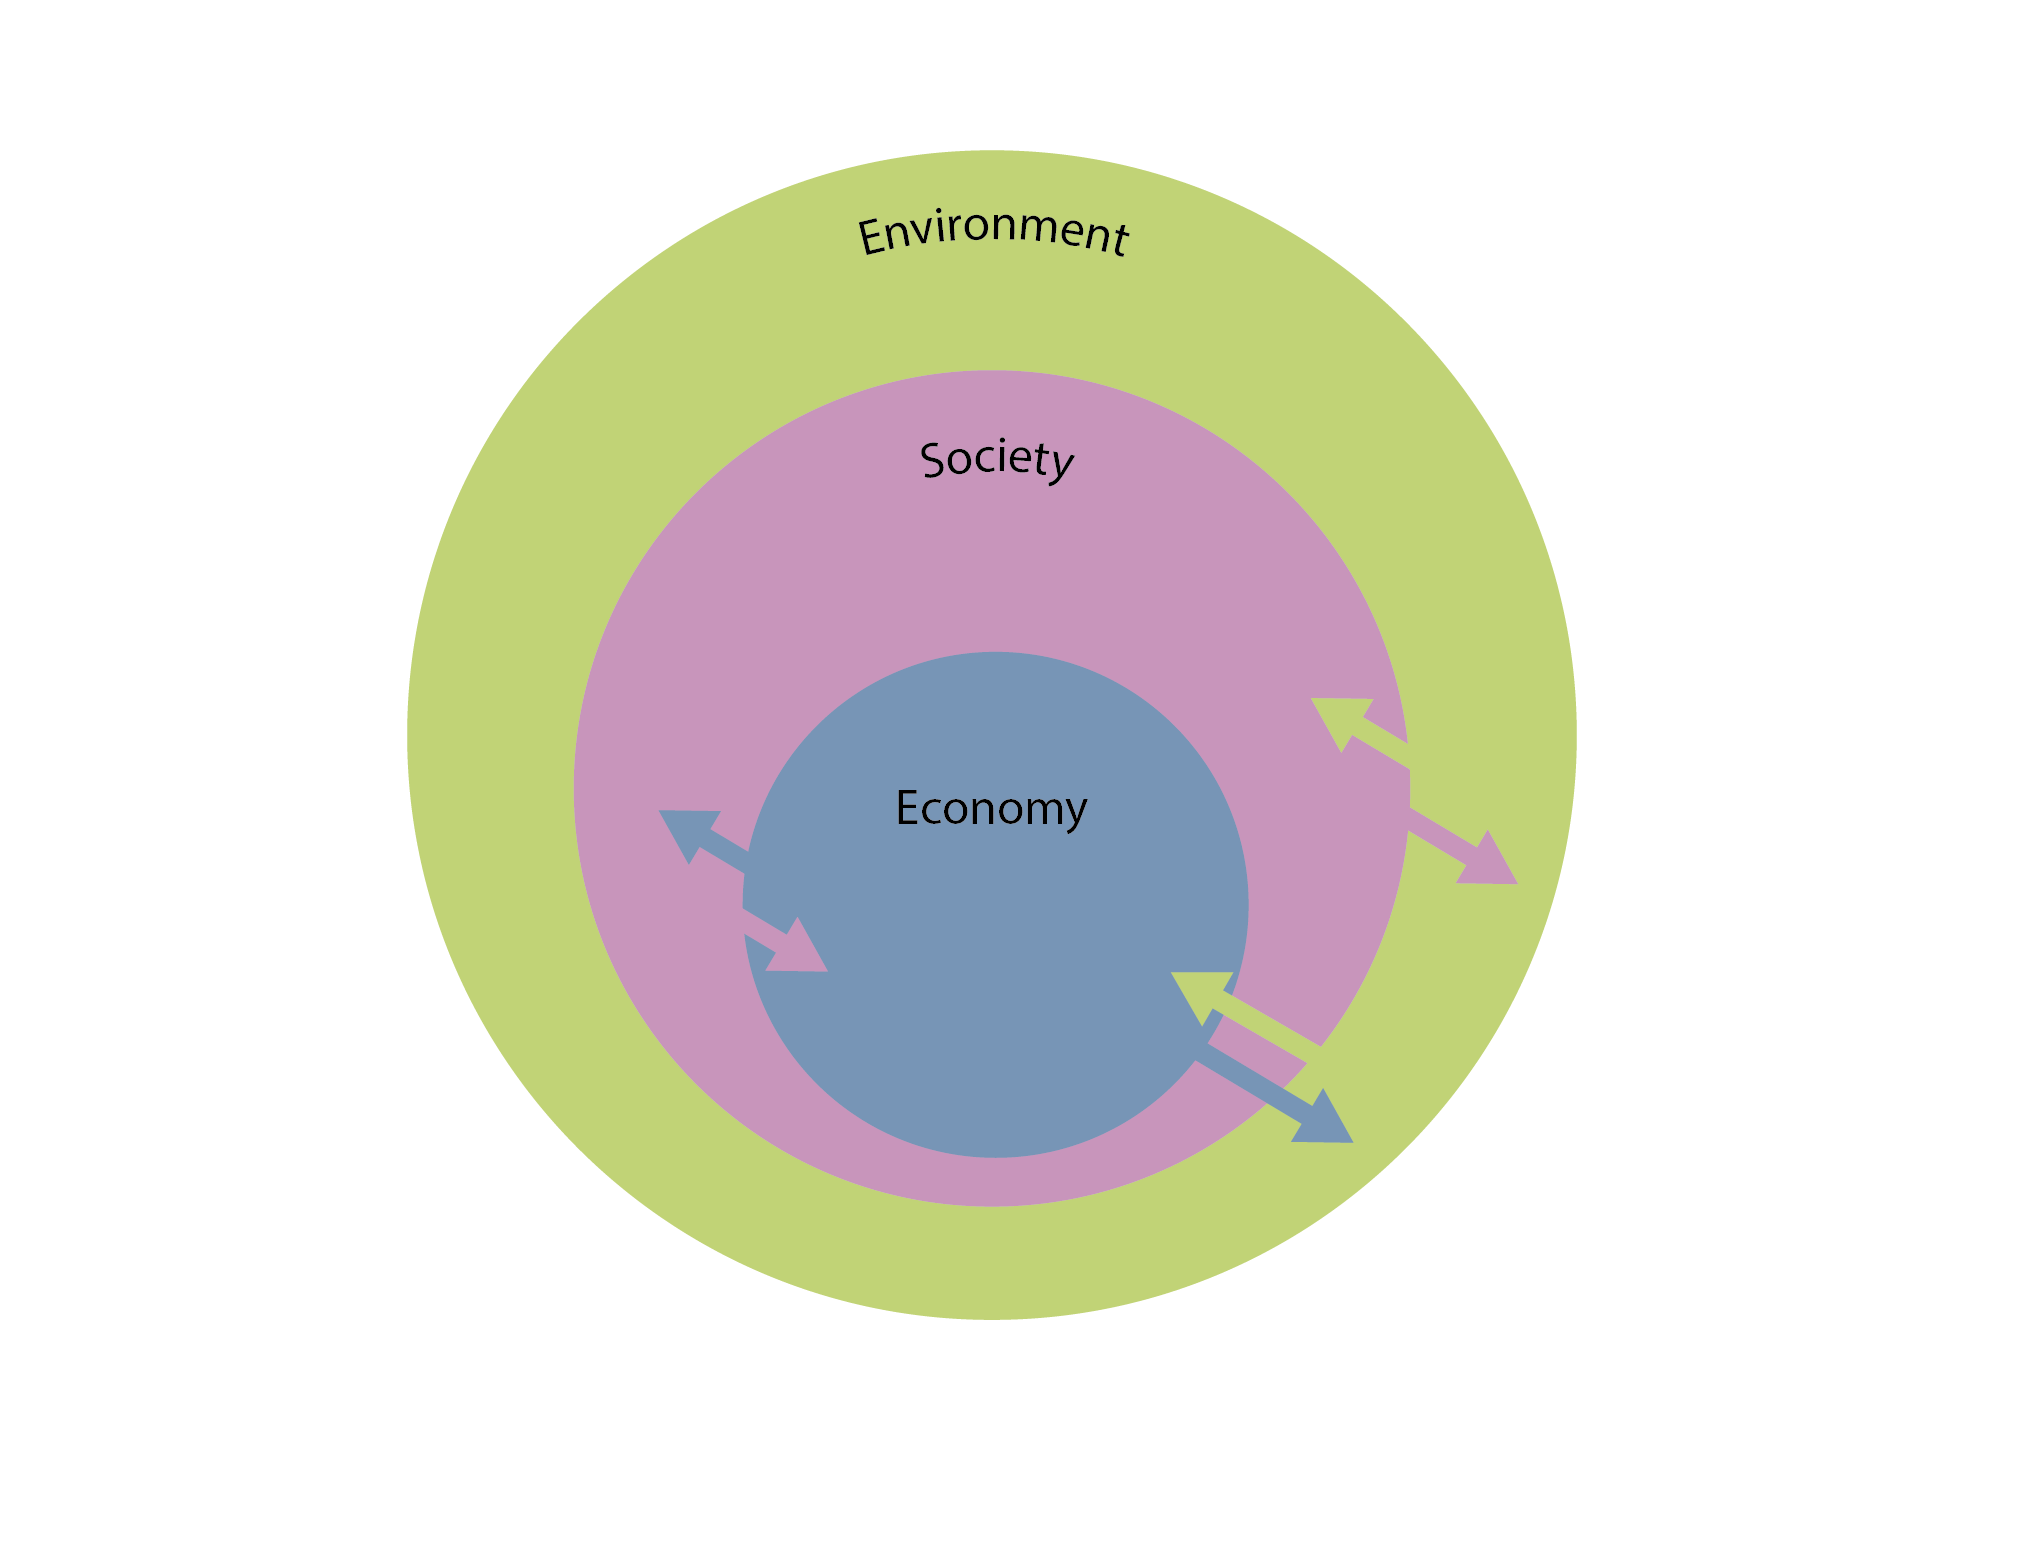
\includegraphics[keepaspectratio]{1_understanding/images/sustainability-nested.png}}

}

\caption{\label{fig-sustainability-nested}Das verschachtelte Modell der
Nachhaltigkeit. Quelle: Eigene Darstellung basierend auf Giddings u.~a.
(2002, pp.~192)).}

\end{figure}%

\subsection{Ein vierdimensionales
Nachhaltigkeitsmodell}\label{ein-vierdimensionales-nachhaltigkeitsmodell}

Ein Problem des Drei-Säulen-Modells der Nachhaltigkeit besteht darin,
dass unklar ist, was unter den weit gefassten „sozialen'' Bereich fällt.
Es wurde daher vorgeschlagen, eine vierte Dimension hinzuzufügen, um
bestimmte Aspekte zu betonen, die sonst im sozialen Sektor verborgen
bleiben könnten. Der australische Kulturkommentator Jon Hawkes hat
beispielsweise vorgeschlagen, „kulturelle Vitalität'' als vierte Säule
der Nachhaltigkeit hinzuzufügen, zusätzlich zu ökologischen,
wirtschaftlichen und sozialen Belangen.

\begin{figure}[H]

\centering{

\pandocbounded{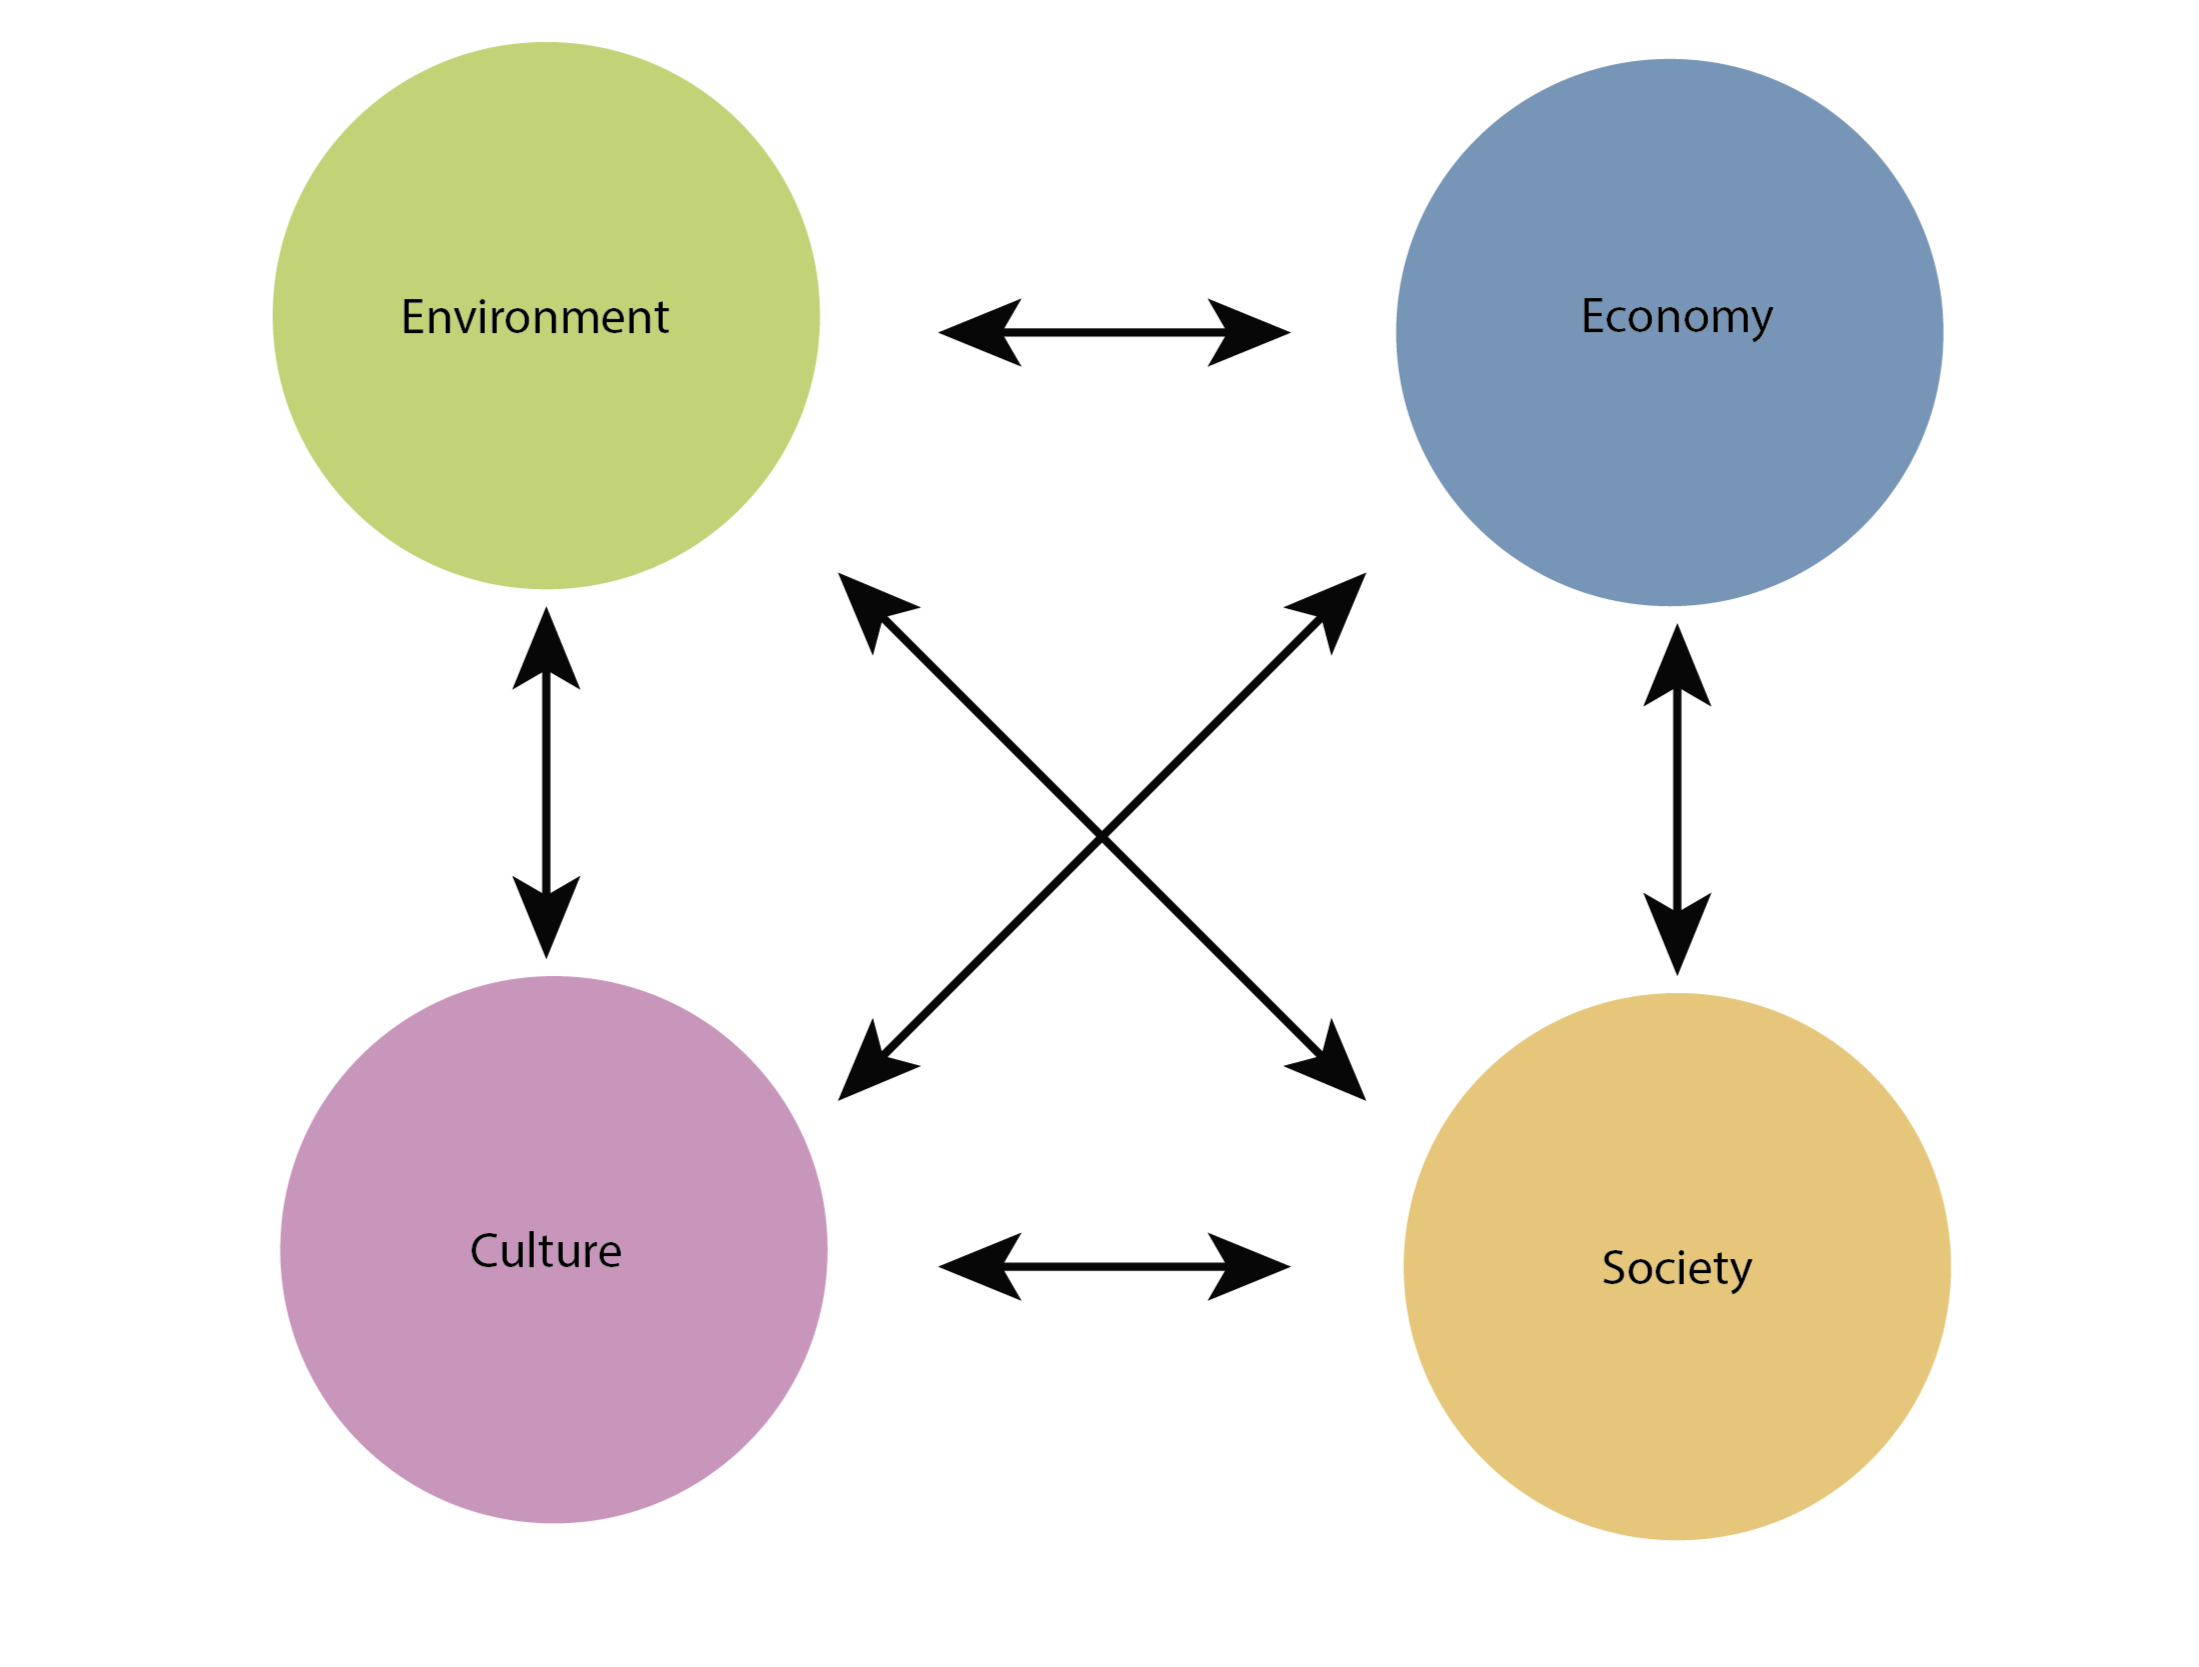
\includegraphics[keepaspectratio]{1_understanding/images/sustainability-4-dimensions.png}}

}

\caption{\label{fig-sustainability-4-dimensions}Vierdimensionales
Nachhaltigkeitsmodell. Quelle: Eigene Darstellung, adaptiert von Hawkes
(2001).}

\end{figure}%

Kulturelle Nachhaltigkeit wird oft als Teil der sozialen Nachhaltigkeit
betrachtet. Manchmal wird auch der Begriff „soziokulturelle
Nachhaltigkeit'' verwendet. In diesem Zusammenhang bezieht sich
„Kultur'' auf Aspekte wie Chancengleichheit,
Partizipationsmöglichkeiten, Nachhaltigkeitsbewusstsein und allgemeine
Betriebs- und Verhaltensmodelle (Murphy 2012). Es ist offensichtlich,
dass die sozialen und kulturellen Dimensionen eng miteinander verknüpft
sind. Kulturelle Prozesse beeinflussen unser soziales Leben und unsere
Sichtweise auf soziale Nachhaltigkeit, wie zum Beispiel den Wert, den
wir Gleichheit als soziales Ziel beimessen. Umgekehrt beeinflussen
soziale Strukturen und Institutionen kulturelle Praktiken und Urteile.
Trotz dieser engen Verbindung können kulturelle und soziale
Nachhaltigkeit auch als separate Dimensionen oder Perspektiven der
Nachhaltigkeit betrachtet werden.

Kultur hat kein eigenes Ziel für Nachhaltige Entwicklung (SDG). In der
Agenda 2030 wird Kultur im Zusammenhang mit „Zivilisation'',
„Diversität'', „Interkulturalität'', „kulturellem Erbe'' und
„Tourismus'' im Rahmen der folgenden vier SDGs erwähnt: Hochwertige
Bildung (SDG 4), Menschenwürdige Arbeit und Wirtschaftswachstum (SDG 8),
Nachhaltige Städte und Gemeinden (SDG 11) und Verantwortungsvoller
Konsum und Produktion (SDG 12) (Duxbury u.~a. 2017).

Das Konzept der kulturellen Nachhaltigkeit kann auf verschiedene Arten
interpretiert werden: als vierte Dimension der Nachhaltigkeit, als
Kultur für Nachhaltigkeit und als Kultur als Nachhaltigkeit. Die
Interpretation „Kultur als Nachhaltigkeit'' erfordert eine neue
Denkweise und ein neues Paradigma in Bezug auf Nachhaltigkeit. In dieser
Sichtweise wird Kultur selbst in Richtung Nachhaltigkeit transformiert.
Kulturelle Nachhaltigkeit bedeutet hier, darüber nachzudenken, was
erhalten werden muss, was sich verändern muss und wie wir diese
Veränderungen umsetzen können. Diese Interpretation -- Kultur als
Nachhaltige Entwicklung zu betrachten -- definiert Kultur im weitesten
Sinne als eine umfassende Lebensweise und einen sich kontinuierlich
verändernden Prozess. Unsere Gesellschaftsordnung (wie Kapitalismus und
Demokratie), unsere Werte und unsere Arbeitsweisen sind allesamt
kulturelle Produkte. Kultur umfasst damit alle anderen Dimensionen der
Nachhaltigkeit, und ihre Transformation wird zu einem zentralen Anliegen
oder Paradigma für die Nachhaltigkeit.

Die Definition der kulturellen Nachhaltigkeit enthält mehrere wichtige
Aspekte: Erstens betont sie die Bedeutung von intellektuellem Wachstum
und Verantwortung. Dies bedeutet, Wissen zu erwerben, ein besseres
Verständnis wichtiger Themen zu entwickeln und an Bildungsaktivitäten
und -veranstaltungen teilzunehmen. Es bedeutet auch, nicht nur als
Einzelperson zu handeln, sondern auch als Mitglied verschiedener
Gemeinschaften. Alle problematischen und nicht nachhaltigen Strukturen
und Betriebsmodelle wurden von Menschen geschaffen und entwickelt. Wir
Menschen haben daher auch die Möglichkeit, sie zu verändern.

Kulturelle Nachhaltigkeit ist beispielsweise für eine „Grosse
Transformation'' erforderlich, wie sie Uwe Schneidewind (2018)
befürwortet. In seinem Werk betont Schneidewind die Notwendigkeit eines
umfassenden Wandels in allen Dimensionen der Gesellschaft,
einschliesslich der Kultur, um Nachhaltige Entwicklung zu erreichen. Die
Anerkennung kultureller Nachhaltigkeit als zentrales Paradigma der
Nachhaltigkeit unterstützt die Vision einer umfassenden Transformation,
die über technologische und wirtschaftliche Lösungen hinausgeht und
einen grundlegenden gesellschaftlichen Kurswechsel anstrebt.

\section{Schwache und starke
Nachhaltigkeit}\label{schwache-und-starke-nachhaltigkeit}

Die wissenschaftliche Debatte zur Nachhaltigkeit unterscheidet zwischen
schwacher und starker Nachhaltigkeit (vgl. z. B. Ott 2020). Keines der
Konzepte lässt sich leicht verwerfen, da beide auf Annahmen beruhen, die
schwer zu widerlegen sind. In der Praxis werden beide Konzepte als
teilweise zutreffend betrachtet, mit Belegen sowohl dafür als auch
dagegen. Der wesentliche Unterschied zwischen schwacher und starker
Nachhaltigkeit liegt in der Frage, was wir erhalten sollten, und in dem
Ausmass, in dem verschiedene Kapitalformen substituierbar sind. Dies
betrifft insbesondere die folgenden drei Kapitalformen: Naturkapital,
Sachkapital und Humankapital.

Naturkapital: die natürlichen Ressourcen und Ökosysteme, die für das
menschliche Wohlbefinden und eine Nachhaltige Entwicklung entscheidend
sind. Dazu gehören Land, Wasser, Luft, Biodiversität und erneuerbare
Energie. Naturkapital bildet die Grundlage für viele wirtschaftliche
Aktivitäten und liefert wesentliche Ökosystemdienstleistungen wie
Nahrung, die Reinigung von Wasser und Luft sowie kulturelle und
ästhetische Leistungen.

Sachkapital: die materiellen Ressourcen und Infrastrukturen, die in
Produktion und Wirtschaftstätigkeit eingesetzt werden. Dazu gehören
Gebäude, Maschinen, technische Ausrüstungen, Transportmittel und
physische Infrastruktur. Sachkapital ist eng mit Wirtschaftswachstum und
Produktivität verknüpft und spielt eine wichtige Rolle in der
wirtschaftlichen Entwicklung.

Humankapital: das Wissen, die Fähigkeiten, der Bildungsstand, die
Gesundheit und die kreativen Fähigkeiten der Menschen in einer
Gesellschaft. Es umfasst individuelles und kollektives Wissen sowie die
Fähigkeiten, die für wirtschaftliche Produktivität und sozialen
Fortschritt benötigt werden. Humankapital ist wichtig für Innovation,
Arbeitsproduktivität, gesellschaftliche Partizipation und die Fähigkeit
einer Gesellschaft, Herausforderungen zu bewältigen und sich anzupassen.

\subsection{Schwache Nachhaltigkeit}\label{schwache-nachhaltigkeit}

Schwache Nachhaltigkeit kann als die „weiche'' oder flexible Option
betrachtet werden. Befürworter*innen der schwachen Nachhaltigkeit sind
der Ansicht, dass eine Massnahme dann nachhaltig ist, wenn sie dem
Gesamtsystem einen Vorteil bietet oder zumindest dessen Qualität nicht
vermindert. Schwache Nachhaltigkeit kann daher als eine grundlegende
Anforderung an die Nachhaltigkeit betrachtet werden, da sie darauf
abzielt, ein bestimmtes Mass an Wohlbefinden/Lebensqualität
aufrechtzuerhalten oder Chancengleichheit zu gewährleisten. Das Konzept
der schwachen Nachhaltigkeit „setzt die weitreichende und zumindest
prinzipiell unbegrenzte {[}\ldots{]} Substituierbarkeit aller
Kapitalarten voraus'' (Ott und Döring 2004, pp.~41) und basiert damit
auf der Prämisse der neoklassischen Ökonomie. Befürworter*innen der
schwachen Nachhaltigkeit glauben, dass Naturkapital durch andere
Kapitalformen ersetzt werden kann. Sie betonen das Konzept des
„Gesamtkapitals'' und argumentieren, dass die spezifische
Zusammensetzung des von zukünftigen Generationen geerbten Kapitals
irrelevant sei, solange der Gesamtnutzen und das Wohlbefinden
aufrechterhalten werden. Dies entspricht der neoklassischen
Nutzwerttheorie, wonach es irrelevant ist, wie Nutzen erzeugt wird.

Befürworter*innen der schwachen Nachhaltigkeit sind daher der Ansicht,
dass Massnahmen auch dann als nachhaltig gelten können, wenn sie auf
Kosten des Naturkapitals durchgeführt werden -- solange dieser Verlust
durch eine Steigerung des Human- oder Sachkapitals kompensiert wird.
Dies könnte den Abbau von Rohstoffen wie Kohle oder übermässigem Rohöl
rechtfertigen. Und Carlowitz' Wald aus der \emph{Sylvicultura
oeconomica} könnte im Prinzip auch ersetzbar oder abbaubar sein, sofern
seine natürlichen und kulturellen Funktionen von zukünftigen
Generationen auf andere Weise erfüllt werden können. Dieses Verständnis
von Nachhaltigkeit betont die Bedeutung des technologischen Fortschritts
für eine Nachhaltige Entwicklung.

Die Bewertung von Massnahmen auf der Grundlage schwacher Nachhaltigkeit
ist aufgrund der immanenten Komplexität und der zahlreichen damit
verbundenen Annahmen schwierig. Dies geht über grundlegende
Nachhaltigkeitsfragen hinaus, wie etwa „Was ist ein gutes Leben?'' oder
„Wie messen wir das Mass an Wohlbefinden?{\kern0pt}``. Eine zentrale
Herausforderung liegt in der monetären Bewertung verschiedener
Kapitalformen, insbesondere solcher ohne klaren Marktpreis. Was soll
dabei berücksichtigt werden? Welchen Wert hat natürliche Schönheit?
Welchen Wert hat ein seltener Vogel oder ein Wal? Bullers \emph{The
Value of a Whale} (2022) zeigt eindrücklich die Probleme auf, mit denen
wir konfrontiert sind, wenn wir versuchen, Elementen der Natur einen
Preis zu geben.

Kritiker*innen des Konzepts der schwachen Nachhaltigkeit weisen auf
mehrere Einschränkungen hin. Erstens hinterfragen sie die Annahme, dass
natürliche Ressourcen endlos durch reproduzierbares Kapital ersetzt
werden können. Zweitens zweifeln sie daran, ob eine Zunahme von Gütern
den Verlust an Umweltqualität tatsächlich kompensieren kann.
Schliesslich bestehen Bedenken hinsichtlich unserer Fähigkeit, neue
Ressourcen zu erschliessen, und der Möglichkeit, kritische
Schwellenwerte zu überschreiten. Diese Kritik hat den Weg für das
Konzept der „starken Nachhaltigkeit'' geebnet.

\subsection{Starke Nachhaltigkeit}\label{starke-nachhaltigkeit}

Im Gegensatz zur schwachen Nachhaltigkeit betont die starke
Nachhaltigkeit die Erhaltung des Naturkapitals. Befürworter*innen dieser
ökozentrischen Theorie sind weniger optimistisch bezüglich unserer
Fähigkeit, natürliche Ressourcen durch hergestellte zu ersetzen, da sie
diese Ressourcentypen als begrenzt austauschbar betrachten (Daly 1990;
Ott 2001; Ott und Döring 2004). Sie argumentieren, dass die einzelnen
Elemente des Naturkapitals so konstant wie möglich gehalten werden
sollten, um beispielsweise das Artensterben zu verhindern.

\begingroup\fontsize{8}{10}\selectfont

\begin{longtable}[t]{>{\raggedright\arraybackslash}p{1.6cm}>{\raggedright\arraybackslash}p{2.3cm}>{\raggedright\arraybackslash}p{2.3cm}>{\raggedright\arraybackslash}p{2.3cm}>{\raggedright\arraybackslash}p{2.3cm}}

\caption{\label{tbl-weak-strong-sustainability}Schwache und starke
Nachhaltigkeit. Quelle: Abgeleitet von Eblinghaus und Stickler (1998);
{Michelsen u.~a.} (2012); und Davies (2013).}

\tabularnewline

\toprule
\textbf{Kategorie} & \textbf{Sehr schwache Nachhaltigkeit} & \textbf{Schwache Nachhaltigkeit} & \textbf{Starke Nachhaltigkeit} & \textbf{Sehr starke Nachhaltigkeit}\\
\midrule
\endfirsthead
\multicolumn{5}{@{}l}{\textit{(continued)}}\\
\toprule
\textbf{Kategorie} & \textbf{Sehr schwache Nachhaltigkeit} & \textbf{Schwache Nachhaltigkeit} & \textbf{Starke Nachhaltigkeit} & \textbf{Sehr starke Nachhaltigkeit}\\
\midrule
\endhead

\endfoot
\bottomrule
\endlastfoot
\textbf{Was soll erhalten werden?} & Gesamtkapital & Wesentliches Naturkapital & Nicht erneuerbares Naturkapital & Die Natur hat einen eigenen Wert\\
\textbf{Warum?} & Maximierung des wirtschaftlichen Gewinns und des individuellen Wohlbefindens (BIP) & + Begrenzung von Umweltschäden und Ressourcenknappheit & Sicherung langfristiger Lebensbedingungen für Menschen und Natur & + Achtung aller Lebensformen und Pflichten gegenüber der Natur\\
\textbf{Wie? (Massnahmen)} & Wachstums­orientierung durch Förderung von Technologie und Innovation & Umweltvorschriften, Ressourceneffizienz, erneuerbare Energien & + Schutzmassnahmen, ökologische Wiederherstellung, nachhaltige Landwirtschaft & –\\
\textbf{Substituier­barkeit} & Im Prinzip unbegrenzt, natürliche Ressourcen können durch Technologie und Handel ersetzt werden & Teilweise möglich, aber begrenzte Substituierbarkeit von Ökosystemdienstleistungen & Begrenzt, kritische Schwelle für Umweltveränderungen & Gering, Anerkennung einzigartiger Werte und Beziehungen\\
\textbf{Ethik} & Anthropozentrisch, kurzfristige Vorteile haben Vorrang & Anthropozentrisch mit stärkerer Berücksichtigung von Umweltinteressen & Pathozentrismus, Anerkennung des immanenten Werts der Natur & Biozentrismus, ökologische Integrität, ethische Verantwortung gegenüber der Natur\\*

\end{longtable}

\endgroup{}

Während neoklassische Ökonom*innen der Substitution zuversichtlich
gegenüberstehen, betonen Vertreter*innen der starken Nachhaltigkeit die
Bedeutung von Prävention und Antizipation statt Nachsorge und Reaktion.
Auf das Ozonloch beispielsweise mit Sonnencreme, Schutzkleidung oder
medizinischer Nachsorge zu reagieren, geht nicht an die Wurzel des
Problems. Ähnlich werden technologische Ansätze wie Geo-Engineering
dafür kritisiert, Probleme nur oberflächlich zu behandeln.
Geo-Engineering bezeichnet technische Eingriffe in geochemische oder
biogeochemische Kreisläufe, um beispielsweise den Klimawandel oder die
Ozeanversauerung zu verlangsamen.

Bisher konzentrierte sich die Verringerung von Umweltverschmutzung
hauptsächlich auf End-of-Pipe-Technologien, wie
Rauchgasreinigungsanlagen an Fabrikschornsteinen oder Katalysatoren in
Autos. Damit wurde aber auch die Bewältigung langfristiger
Umweltprobleme wie dem Klimawandel oder dem Biodiversitätsverlust
aufgeschoben, solange ihre Auswirkungen nicht unmittelbar spürbar waren.
Dieses Phänomen ist mit dem Konzept der Externalisierung verbunden, bei
dem Umwelt- und Sozialkosten nach aussen verlagert werden, wie es
Lessenich (2018) beschreibt. Dies bedeutet, dass bei der Preisgestaltung
nur die wirtschaftlichen Kosten berücksichtigt werden, teilweise weil
sie leichter zu quantifizieren sind, während die sozialen und
ökologischen Kosten der Bereitstellung von Gütern und Dienstleistungen
weggelassen oder externalisiert werden, was zu Verzerrungen der
Marktpreise führt.

\section{Nachhaltigkeitsstrategien als Prinzipien Nachhaltiger
Entwicklung}\label{nachhaltigkeitsstrategien-als-prinzipien-nachhaltiger-entwicklung}

\begin{figure}[H]

\centering{

\pandocbounded{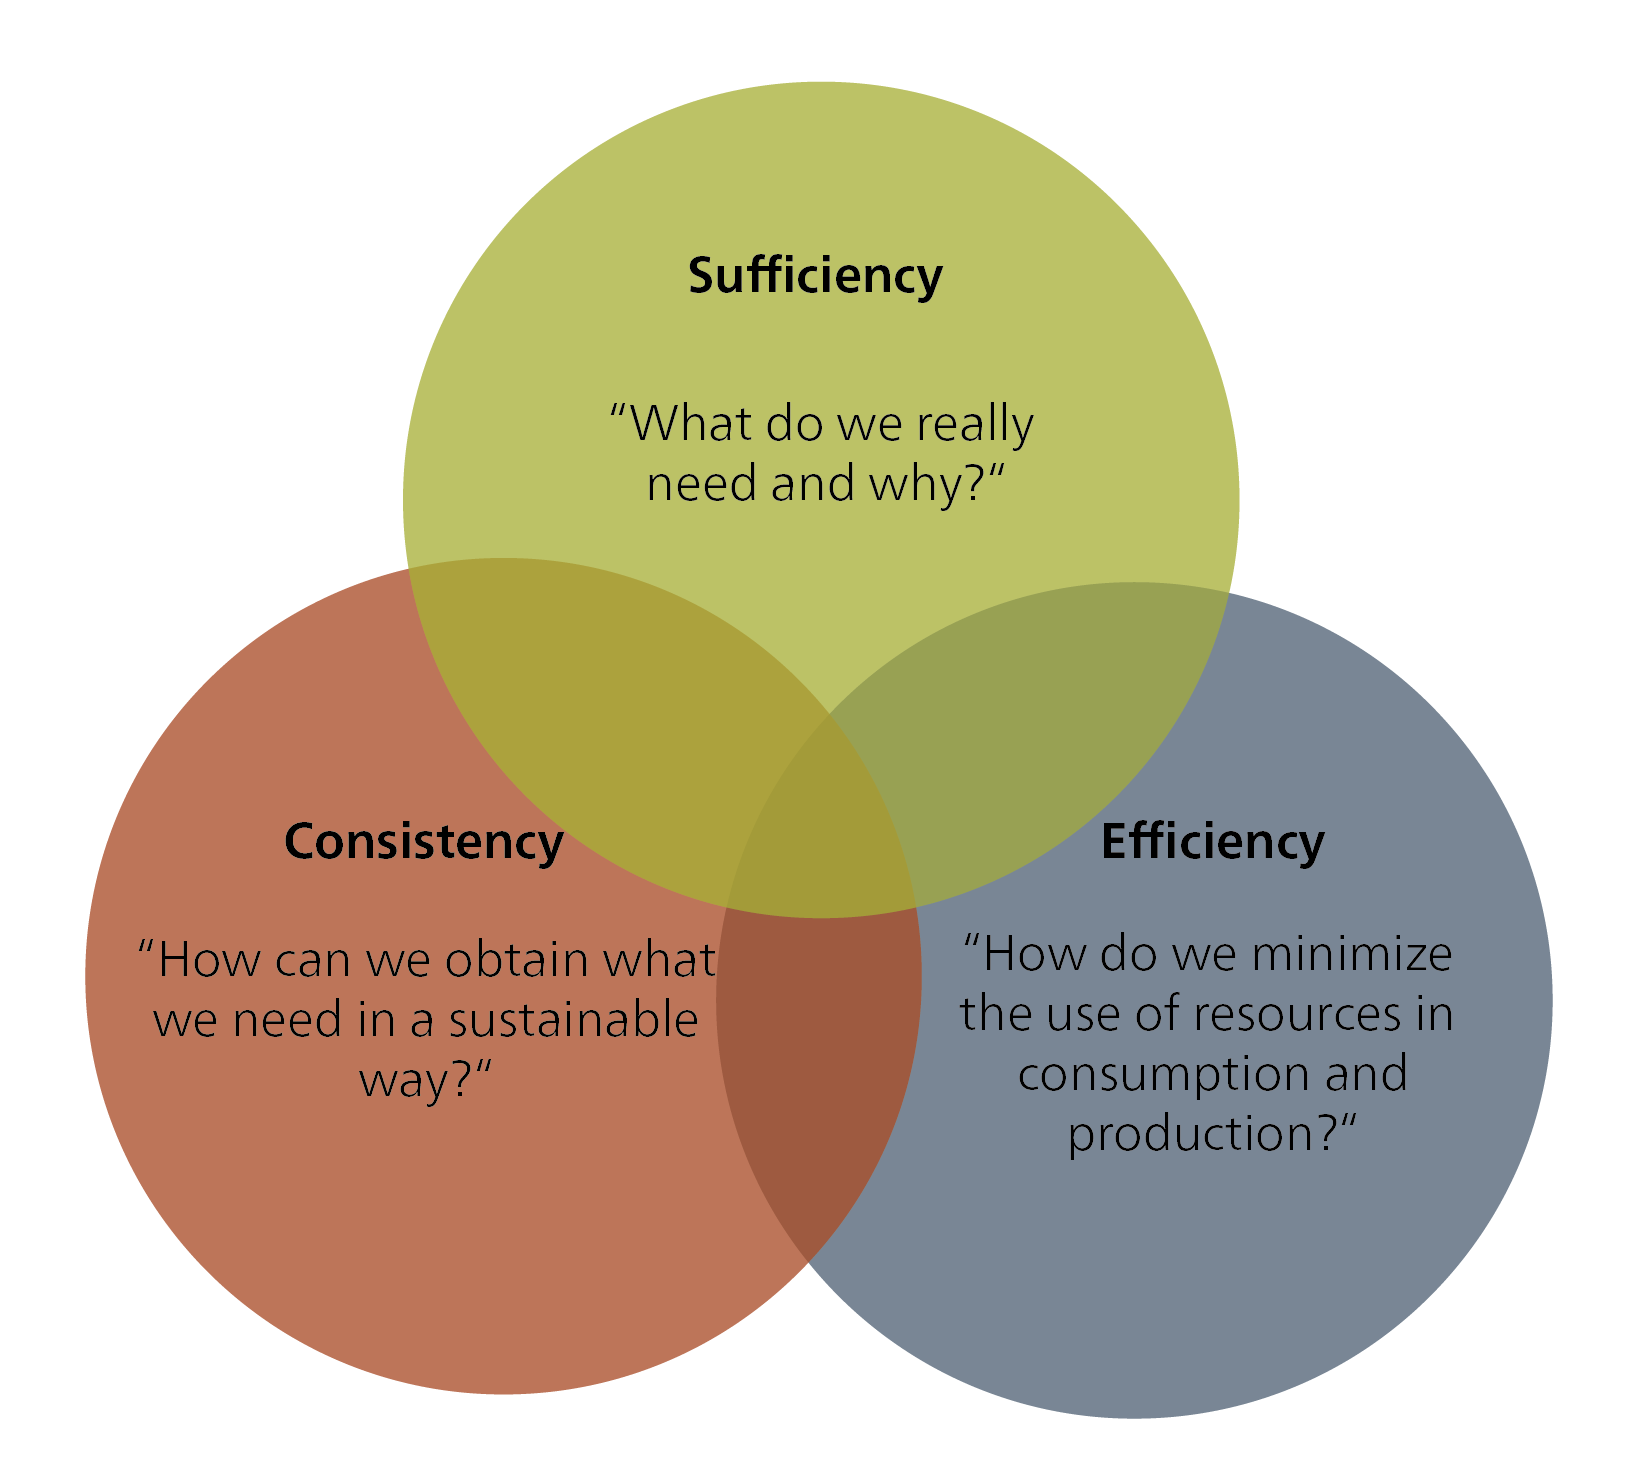
\includegraphics[keepaspectratio]{1_understanding/images/Fig1_12_sustainability-strategies.png}}

}

\caption{\label{fig-sustainability-strategies}Nachhaltigkeitsstrategien.
Quelle: Eigene Darstellung.}

\end{figure}%

\subsection{Effizienzstrategie}\label{effizienzstrategie}

Die Effizienzstrategie konzentriert sich auf die Minimierung des
Ressourceneinsatzes (d.~h. Rohstoffe und Energie) bei der Herstellung
oder Erbringung von Dienstleistungen. Dies bedeutet die Reduzierung des
Materialverbrauchs (Materialintensität), des Energieverbrauchs
(Energieintensität) und der Emissionen von Schadstoffen wie
CO\textsubscript{2}. Diese auch als „Ökoeffizienz'' bekannte Strategie
ist für Wirtschaft und Gesellschaft attraktiv, da sie Kosten,
Ressourcenverbrauch und Umweltbelastung senken kann. Die Umsetzung der
Effizienzstrategie beginnt mit der Verbesserung von
Produktionsprozessen, in erster Linie durch technologische Fortschritte.
Befürworter*innen glauben, dass es möglich ist, den Wohlstand zu
verdoppeln und gleichzeitig den Naturressourcenverbrauch zu halbieren
({von Weizsäcker u.~a.} 1995). Kritiker*innen der Effizienzstrategie
sind jedoch weniger optimistisch und warnen davor, ihre Wirkung auf eine
nachhaltige Wirtschaftstätigkeit zu überschätzen. Sie verweisen auf
„Rebound-Effekte'', die die Gewinne aus Effizienzsteigerungen verringern
oder sogar zunichte machen können (Paech 2012; Santarius 2014).

\begin{tcolorbox}[enhanced jigsaw, arc=.35mm, bottomrule=.15mm, bottomtitle=1mm, breakable, colback=white, colbacktitle=quarto-callout-tip-color!10!white, colframe=quarto-callout-tip-color-frame, coltitle=black, left=2mm, leftrule=.75mm, opacityback=0, opacitybacktitle=0.6, rightrule=.15mm, title={Effizienzstrategien in der Praxis: Beispiele}, titlerule=0mm, toprule=.15mm, toptitle=1mm]

\textbf{Energieeffiziente Beleuchtung}: Der Ersatz herkömmlicher
Glühbirnen durch energieeffiziente LED-Leuchtmittel senkt den
Stromverbrauch und hilft, den Energiebedarf zu reduzieren.

\textbf{Kraftstoffeffiziente Fahrzeuge}: Die Entwicklung von
kraftstoffeffizienteren Hybrid- oder Elektrofahrzeugen kann zu einem
geringeren Kraftstoffverbrauch und niedrigeren Emissionen im
Strassenverkehr führen.

\textbf{Effiziente Gebäudetechnik}: Die Installation intelligenter
HLK-Systeme (Heizung, Lüftung und Klimatisierung) in Gebäuden hilft, den
Energieverbrauch für Heizung und Kühlung zu reduzieren.

\textbf{Effizienter Wasserverbrauch}: Der Einsatz wassersparender
Armaturen und Systeme in Haushalten und Industrieunternehmen reduziert
den Wasserverbrauch und minimiert Abfälle.

\end{tcolorbox}

\subsection{Konsistenzstrategie}\label{konsistenzstrategie}

Während die Effizienzstrategie sich auf die Quantität konzentriert
(Reduzierung des Ressourceneinsatzes bei gleichzeitig grösserem Output),
strebt die Konsistenzstrategie (vom Lateinischen \emph{con} = zusammen +
\emph{sistere} = anhalten) danach, Natur und Technik zu versöhnen, indem
Ressourcen wiederholt statt nur einmal genutzt werden. Anstelle fossiler
Ressourcen, Produkte und Technologien sollen Materialien eingesetzt
werden, die mit natürlichen Stoffkreisläufen und -prozessen kompatibel
sind. Dieses auch als „Ökoeffektivität'' bezeichnete Konzept folgt dem
Prinzip „von der Wiege zur Wiege'' (\emph{cradle to cradle}) statt „von
der Wiege zur Bahre'' (\emph{cradle to grave}) und basiert auf der Idee,
dass intelligente Systeme nur Produkte, keinen Abfall erzeugen. Dies
kann auf zwei Wegen erreicht werden: Materialien können entweder
biologisch abbaubar sein (z. B. ein Shampoo aus natürlichen
Inhaltsstoffen) oder sie können mit „technischen Nährstoffen'' gestaltet
werden, die im technischen Kreislauf verbleiben. Das bedeutet, dass ein
ausgedienter Gegenstand nicht im Abfall landet, sondern in den nächsten
Nutzungskreislauf eintritt, beispielsweise durch Upcycling (z. B.
Wiederverwendung eines Computergehäuses oder Umbau zu einem
Regalsystem). Wie die Effizienzstrategie beginnt auch die
Konsistenzstrategie damit, zu prüfen, wie Produktionsprozesse optimiert
werden können. Viele sind der Ansicht, dass die Konsistenzstrategie ein
grösseres Potenzial als die Effizienzstrategie hat, wenn es um die
Problemlösung und das Erreichen weitreichender Veränderungen geht.

Kritiker*innen halten die Theorie jedoch für begrenzt anwendbar. Gerolf
Hanke und Benjamin Best (2013) argumentieren beispielsweise, dass sie
nicht gleichermaassen auf jeden Gütertyp angewendet werden kann und dass
die Umsetzung entsprechender Technologien erhebliche Investitionen in
Produktionsanlagen und Logistik erfordern würde. Sie weisen auch darauf
hin, dass Recyclingprozesse selbst mit einem erhöhten Energieverbrauch
verbunden sind, gemäss dem Entropiegesetz:

\begin{quote}
„Jeder materielle Wirtschaftsprozess führt zu einer Zunahme der
Entropie, d.~h. vereinfacht ausgedrückt, dass die Elemente auf
materieller Ebene immer gleichmässiger verteilt werden, was letztlich
nur bedeutet, dass Dinge und Körper sich abnutzen und eine neue
Konzentration immer mehr Energie erfordert.'' (Übersetzt aus Hanke und
Best 2013, pp.~11)
\end{quote}

Eine Besonderheit des Ökosystems Erde ist die Sonnenenergie, die von
aussen eine konstante Energiezufuhr liefert und der Zunahme der Entropie
auf der Erde entgegenwirkt. Wir benötigen jedoch weiterhin sogenannte
„graue Energie'', um Energieerzeugungssysteme herzustellen, z. B.
Biokraftstoffsysteme, Solarzellen, Elektroautobatterien und
Windturbinen. Konsistenzstrategien können die Industrie anreizen, eine
Reduzierung des Ressourcenverbrauchs und der Emissionen anzustreben.

\begin{tcolorbox}[enhanced jigsaw, arc=.35mm, bottomrule=.15mm, bottomtitle=1mm, breakable, colback=white, colbacktitle=quarto-callout-tip-color!10!white, colframe=quarto-callout-tip-color-frame, coltitle=black, left=2mm, leftrule=.75mm, opacityback=0, opacitybacktitle=0.6, rightrule=.15mm, title={Konsistenzstrategien in der Praxis: Beispiele}, titlerule=0mm, toprule=.15mm, toptitle=1mm]

\textbf{Erneuerbare Energiesysteme}: Der Übergang von fossilen
Brennstoffen zu erneuerbaren Energiequellen wie Solar-, Wind- und
Wasserkraft ist ein Bestreben, die Energieerzeugung mit den natürlichen
Rhythmen und Kreisläufen der Umwelt in Einklang zu bringen.

\textbf{Recycelbare Elektronik}: Elektronische Geräte so zu gestalten,
dass sie leicht repariert, aufgerüstet und recycelt werden können, um
den Ressourcenverbrauch und die Umweltbelastung zu minimieren.

\textbf{Nachhaltiges Bauen}: Errichtung von Gebäuden aus nachhaltigen
Materialien, die eine geringe Umweltbelastung aufweisen und am Ende
ihrer Nutzungsdauer wiederverwendet oder recycelt werden können.

\end{tcolorbox}

\subsection{Suffizienzstrategie}\label{suffizienzstrategie}

Das Konzept der Suffizienz, das im lateinischen Wort \emph{sufficere}
(genügen) verwurzelt ist, stellt unsere Annahmen darüber in Frage, wie
viel wir für ein gutes Leben brauchen. Es fördert eine Reduzierung des
Ressourcen- und Energieverbrauchs durch die Fokussierung auf die Senkung
der Nachfrage nach ressourcenintensiven Gütern und Dienstleistungen.
Suffizienz -- die man auch als Genügsamkeit oder Angemessenheit
beschreiben könnte -- kritisiert die ständige Schaffung neuer
Bedürfnisse durch Technologie und Werbung angesichts eines begrenzten
Angebots an natürlichen Ressourcen. Suffizienz mahnt uns, nicht jedem
neu geschaffenen Bedürfnis nachzujagen und unsere Bedürfnisse ohne
Konsum zu erfüllen. Während sich Effizienz- und Konsistenzstrategien auf
die Produktion konzentrieren, richtet sich die Suffizienzstrategie auf
den Konsum -- wenn auch nicht ausschliesslich: Suffizienz kann in
unterschiedlichem Ausmass und auf verschiedenen Ebenen praktiziert
werden, von kleinen Verhaltensänderungen (Teilen statt Kaufen) bis hin
zu erheblichen Änderungen des Lebensstils (Verzicht auf Flugreisen).
Obwohl sie auf individueller Ebene beginnt, kann Suffizienz auf
verschiedenen Ebenen angewendet werden, etwa von Unternehmen
(suffizienzorientiertes Produktdesign) und Regierungen
(Suffizienzpolitik). Suffizienz strebt daher die richtige Balance an:
Wie viel brauchen wir für ein gutes Leben? Und was brauchen wir nicht?

Kritiker*innen sind der Ansicht, dass die Suffizienzstrategie nur
begrenzte Potenziale hat und keine breite soziokulturelle Akzeptanz
finden wird. Befürworter*innen hingegen sehen sie als entscheidend für
die Nachhaltigkeitspolitik, insbesondere dort, wo Effizienz- und
Konsistenzstrategien nicht ausreichen. Das Konzept einer
Postwachstumswirtschaft stützt sich auf die Prinzipien der
Suffizienzstrategie.

\begin{tcolorbox}[enhanced jigsaw, arc=.35mm, bottomrule=.15mm, bottomtitle=1mm, breakable, colback=white, colbacktitle=quarto-callout-tip-color!10!white, colframe=quarto-callout-tip-color-frame, coltitle=black, left=2mm, leftrule=.75mm, opacityback=0, opacitybacktitle=0.6, rightrule=.15mm, title={Suffizienzstrategien in der Praxis: Beispiele}, titlerule=0mm, toprule=.15mm, toptitle=1mm]

\textbf{Teilen und gemeinschaftliche Nutzung}: Plattformen und
Initiativen zum Teilen von Gegenständen, Werkzeugen oder Fahrzeugen
ermöglichen eine effizientere Ressourcennutzung und reduzieren die
Anzahl der hergestellten Produkte.

\textbf{Pflanzenbasierte Ernährung}: Die Umstellung auf eine überwiegend
pflanzliche Ernährung reduziert den Ressourcenverbrauch, z. B. von
Wasser und Land, im Vergleich zur Fleischproduktion.

\textbf{Arbeitszeitverkürzung}: Eine Reduzierung der Arbeitszeit kann zu
einem geringeren Ressourcenverbrauch führen, da weniger Energie und
Materialien für die Produktion von Gütern und Dienstleistungen benötigt
werden.

\textbf{Lokaler Konsum}: Die Unterstützung lokaler Produzent*innen und
Märkte hilft, Transportwege und Emissionen zu reduzieren.

\end{tcolorbox}

\subsection{Rebound-Effekte: Die Kehrseite der
Effizienz}\label{rebound-effekte-die-kehrseite-der-effizienz}

\begin{figure}

\begin{minipage}[t]{0.50\linewidth}

\begin{figure}[H]

\centering{

\pandocbounded{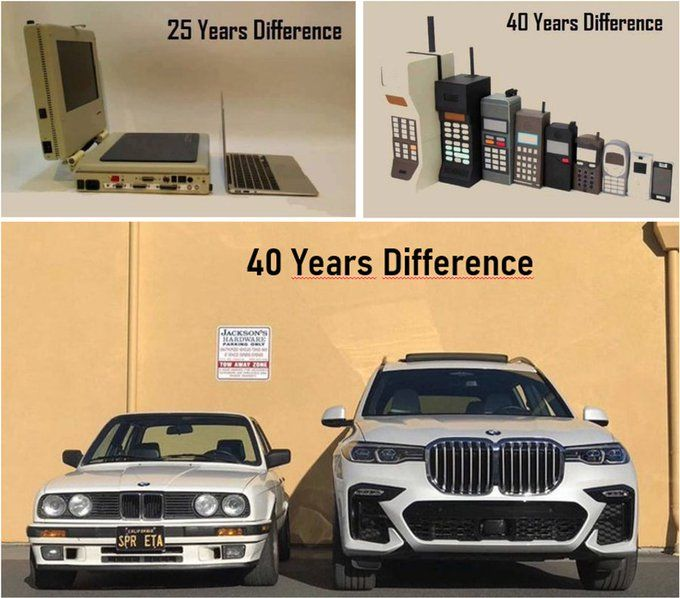
\includegraphics[keepaspectratio]{1_understanding/images/rebound-effect-fietsprofessor.jpg}}

}

\caption{\label{fig-rebound-effect-fietsprofessor}Rebound-Effekt am
Beispiel der Automobilindustrie illustriert. Quelle:
\href{https://www.linkedin.com/posts/brommelstroet_any-intelligent-fool-can-make-things-bigger-activity-7093961897523204096-J7A4?utm_source=share&utm_medium=member_desktop&rcm=ACoAAES-3CUB7iVY2K4QzAF6kE22k9i-b_9D8T0}{@fietsprofessor}
auf LinkedIn.}

\end{figure}%

\end{minipage}%
%
\begin{minipage}[t]{0.50\linewidth}

\begin{quote}
„Jeder intelligente Narr kann Dinge grösser, komplexer und gewaltsamer
machen. Es braucht einen Hauch von Genie -- und viel Mut, um in die
entgegengesetzte Richtung zu gehen.'' (Schumacher 1973)
\end{quote}

\end{minipage}%

\end{figure}%

Kritiker*innen des Effizienzprinzips warnen vor dem Rebound-Effekt, auch
bekannt als Jevons-Paradoxon (Jevons 1865/1965). Dieses Phänomen tritt
auf, wenn Effizienzverbesserungen zu niedrigeren Preisen für Güter und
Dienstleistungen führen, dadurch die Nachfrage steigern und so die
anfänglichen Vorteile eines geringeren Ressourcenverbrauchs
zunichtemachen.

Nehmen wir dieses einfache Beispiel: Wenn Personenwagen durch
Effizienzverbesserungen günstiger werden, wählen Menschen beim nächsten
Kauf möglicherweise ein grösseres Modell. Ausserdem ist ein
kraftstoffeffizientes Auto günstiger im Betrieb, da es weniger
Kraftstoff pro Kilometer benötigt. Dies incentiviert die Menschen
normalerweise dazu, mehr zu fahren (entweder durch häufigere Fahrten
oder längere Strecken) und öffentliche Verkehrsmittel oder das Fahrrad
seltener zu nutzen. Infolgedessen werden technisch mögliche
Effizienzgewinne in der Praxis oft nicht realisiert, da das betreffende
Produkt häufiger oder intensiver genutzt wird. Abgesehen von der
direkten Änderung der Nutzung des Produkts (direkter Rebound) kann es zu
weiteren Änderungen im Konsumverhalten geben, die sich auf die Umwelt
auswirken. In diesem Beispiel könnte das bedeuten, dass das beim Kauf
oder Betrieb des Autos eingesparte Geld stattdessen für Flugreisen
ausgegeben wird (indirekter Rebound), was wiederum einen Teil der
Umweltvorteile zunichtemacht.

\begin{figure}[H]

\centering{

\pandocbounded{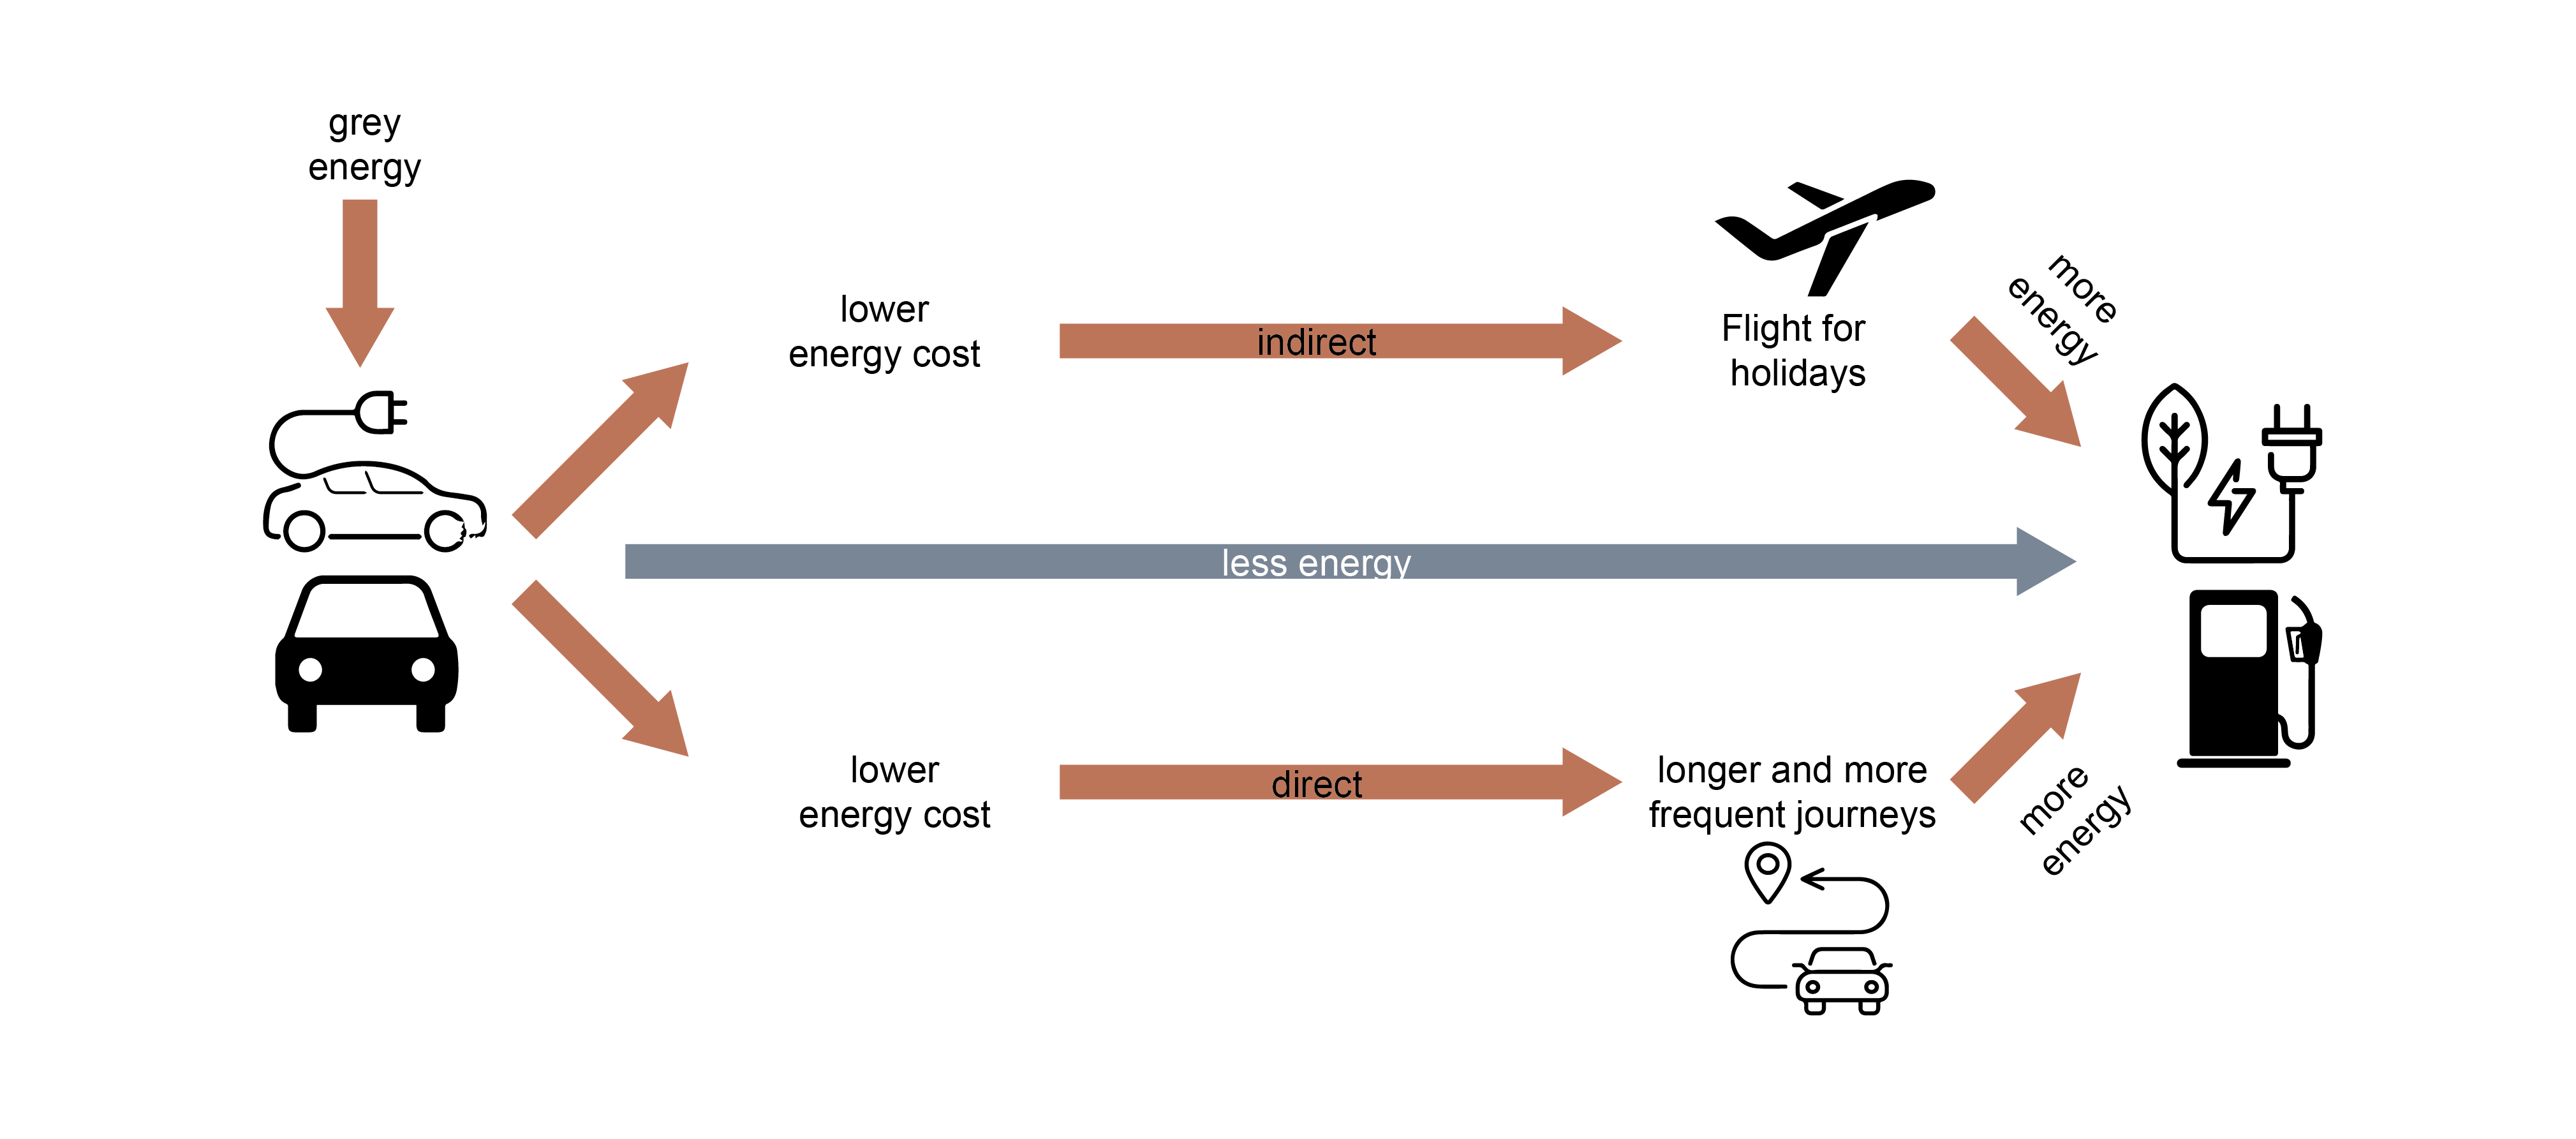
\includegraphics[keepaspectratio]{1_understanding/images/rebound-effect.png}}

}

\caption{\label{fig-rebound-effect}Indirekte und direkte Rebound-Effekte
energiesparender Personenwagen. Quelle: Eigene Darstellung.}

\end{figure}%

Zum Verständnis des Rebound-Effekts konzentriert sich die Literatur auf
die folgenden drei Bereiche: 1) finanzielle Faktoren, 2)
sozialpsychologische Einflüsse und 3) regulatorische Effekte, die wir im
Folgenden eingehender analysieren.

\begin{enumerate}
\def\labelenumi{\arabic{enumi}.}
\tightlist
\item
  Finanzielle Faktoren sind eine wesentliche Ursache des
  Rebound-Effekts. Wenn Effizienz zu Kosteneinsparungen führt, werden
  finanzielle Mittel freigesetzt. Dies kann dazu führen, dass Menschen
  entweder mehr von demselben Produkt konsumieren (direkter
  Rebound-Effekt) oder in alternative Güter investieren (indirekter
  Rebound-Effekt). Der finanzielle Rebound-Effekt kann auf mehreren
  Faktoren beruhen, darunter:

  \begin{itemize}
  \item
    Der Einkommenseffekt: Wenn Effizienz zu realen Einkommenszuwächsen
    für Verbraucher*innen führt, kann dies einen direkten oder
    indirekten Rebound-Effekt bewirken.
  \item
    Der Reinvestitionseffekt: Wenn Unternehmen Kosteneinsparungen
    nutzen, um ihre Produktion auszuweiten oder in andere Produkte zu
    investieren.
  \item
    Der Marktpreiseffekt: Der makroökonomische Effekt, bei dem die
    Nachfrage in einem Sektor die Nachfrage in anderen Sektoren anregt.
    Wenn Autos beispielsweise effizienter werden, kann die Nachfrage
    nach Kraftstoff sinken, was Kraftstoff billiger macht und die
    Nachfrage in anderen energieverbrauchenden Sektoren beeinflusst.
  \end{itemize}
\end{enumerate}

Das Ausmass und die Intensität des finanziellen Rebound-Effekts hängen
von Faktoren wie Preiselastizität und Konsumverhalten ab. Während dies
auf individueller Ebene geschieht, kann es sich zu einem
makroökonomischen Marktpreiseffekt mit weitreichenden Konsequenzen
kumulieren.

\begin{enumerate}
\def\labelenumi{\arabic{enumi}.}
\setcounter{enumi}{1}
\item
  Sozialpsychologische Einflüsse umfassen das „mentale Buchhalten'' der
  einzelnen Verbraucher*innen. Verbraucher*innen, die ein effizientes
  Produkt gekauft haben, „gestatten sich'' beispielsweise
  möglicherweise, mehr zu konsumieren. Deshalb können
  Effizienzsteigerungen bei Produkten, die zuvor als umweltschädlich
  galten, paradoxerweise zu einem Anstieg des Konsums führen. Dieser
  direkte Rebound-Effekt wird in der Sozialpsychologie oft als
  „Moral-Hazard-Effekt'' bezeichnet. Wenn die Entscheidung, den Konsum
  zu steigern, nicht rational getroffen wird, spricht man vom
  „Moral-Leaking-Effekt''. Zum Beispiel, wenn man nach dem Kauf eines
  ressourceneffizienten Autos mehr fährt, weil allein der Kauf als
  umweltbewusst wahrgenommen wird. Auch der indirekte Rebound-Effekt
  kann auf sozialpsychologische Faktoren zurückgeführt werden. Der
  „Moral-Licensing-Effekt'' besagt, dass der Kauf ressourceneffizienter
  Produkte zu einem Anstieg des Konsums anderer Produkte führen kann,
  die möglicherweise umweltschädlich sind. Zum Beispiel, wenn der Kauf
  eines kraftstoffsparenden Autos häufigere Flugreisen rechtfertigt.
\item
  Manchmal können staatliche Regulierungen oder Anreize zur Förderung
  effizienter Technologien unbeabsichtigte Konsequenzen haben -- das
  bezeichnen wir als „regulatorischen Effekt''. Wenn Menschen
  beispielsweise durch staatliche Anreize für energieeffiziente Modelle
  zum Kauf grosser Elektrogeräte animiert werden. Solche Anreize können
  zu häufigeren Käufen von Geräten führen, was -- selbst wenn das neuere
  Modell effizienter ist als das alte -- den Energieeinspareffekt
  teilweise aufhebt. Darüber hinaus führt die Einführung von
  Effizienztechnologien zu neuen Kapazitäten und Infrastrukturen, was
  zur Entstehung neuer Märkte führen kann. Windkraftanlagen
  beispielsweise fördern die Entwicklung neuer Infrastrukturen und
  Arbeitsplätze, benötigen aber gleichzeitig erhebliche Ressourcen.
  Ausserdem müssen Verbraucher*innen, die ein effizienteres Produkt
  kaufen, ihr altes Produkt nicht unbedingt entsorgen. Einige nutzen am
  Ende beide Produkte, was zu einem insgesamt höheren Gesamtkonsum
  führen kann (Santarius 2014).
\end{enumerate}

\begin{tcolorbox}[enhanced jigsaw, arc=.35mm, bottomrule=.15mm, bottomtitle=1mm, breakable, colback=white, colbacktitle=quarto-callout-note-color!10!white, colframe=quarto-callout-note-color-frame, coltitle=black, left=2mm, leftrule=.75mm, opacityback=0, opacitybacktitle=0.6, rightrule=.15mm, title={Rebound-Effekte}, titlerule=0mm, toprule=.15mm, toptitle=1mm]

Der \textbf{direkte Rebound-Effekt} tritt auf, wenn verbesserte
Energieeffizienz den Konsum einer Ressource günstiger macht, was dazu
führt, dass Menschen mehr davon konsumieren. Beispielsweise wäre ein
kraftstoffeffizienteres Auto günstiger im Betrieb. Dies könnte Menschen
dazu veranlassen, mehr zu fahren, und so die Energieeinsparungen durch
die Effizienzsteigerung teilweise oder vollständig zunichtemachen.

Der \textbf{indirekte Rebound-Effekt} tritt auf, wenn
Energieeinsparungen oder Ressourceneffizienzgewinne in einem Bereich zur
Nutzung der freigesetzten Ressource in einem anderen Bereich führen.
Dies reduziert die insgesamt erzielten Einsparungen. Wenn beispielsweise
das durch energieeffizienteres Wohnen eingesparte Geld stattdessen für
häufigere Flugreisen verwendet wird.

\end{tcolorbox}

\subsection{Wie gross ist der
Rebound-Effekt?}\label{wie-gross-ist-der-rebound-effekt}

Es ist schwierig, genau zu bestimmen, wie gross der Rebound-Effekt ist:
Empirische Schätzungen variieren stark, je nach den verwendeten Methoden
und den berücksichtigten Effekten. Es ist besonders schwierig,
Rebound-Effekte klar von Wachstums- oder Strukturveränderungen
abzugrenzen. Die Art der angebotenen Produkte und Dienstleistungen
beeinflusst ebenfalls das Ausmass des Rebound-Effekts. Zum Beispiel:
Wenn ein sparsameres Transportmittel für den täglichen Arbeitsweg
genutzt wird, wie ein effizienteres Auto, sinken die Kosten, aber die
verfügbare Zeit bleibt begrenzt. Man kann daher nicht beliebig oft oder
lange pendeln, da ein Tag nur 24 Stunden hat. Der Rebound-Effekt ist in
diesem Fall also relativ gering. Anders verhält es sich bei
Freizeitaktivitäten wie dem Fliegen. Wenn die Kosten durch effizientere
Flugzeuge oder günstigere Preise sinken, gibt es einen grösseren Anreiz,
häufiger zu fliegen -- beispielsweise statt einer auch mal zwei
Wochenendreisen pro Jahr zu unternehmen. Da Zeit hier keine so knappe
Ressource ist, kann der Zusatzkonsum erheblich steigen -- und damit auch
der Rebound-Effekt. Eine weitere wichtige Komponente ist der
Sättigungsgrad mit Gütern und Dienstleistungen. Beobachtungen zeigen,
dass Rebound-Effekte in Hocheinkommensländern tendenziell geringer sind
als in Entwicklungsländern, wo noch erheblicher Bedarf an zusätzlichem
Konsum besteht.

Die direkten Rebound-Effekte im Zusammenhang mit Effizienzverbesserungen
bei der Raumheizung könnten beispielsweise dazu führen, dass 10--30
Prozent weniger Energie eingespart wird als technisch möglich (vgl.
Hediger u.~a. 2018). Die Rebound-Effekte im Verkehr variieren noch
stärker. Gemäss Andersson u.~a. (2019) könnte der Rebound-Effekt im
Zusammenhang mit privater Mobilität die potenziellen Einsparungen um 7,5
Prozent in Dänemark, 30 Prozent in Schweden und 60 Prozent in
Deutschland reduzieren. Im Gegensatz dazu wurden bei der Beleuchtung in
Privathaushalten sehr geringe Rebound-Effekte von weniger als 10 Prozent
festgestellt (Sorrell 2007). Das bedeutet, dass die tatsächlichen
Energieeinsparungen für diese Dienstleistungen im Durchschnitt bis zu 25
Prozent geringer sein können als technisch möglich und prognostiziert.
Das genaue Ausmass des Rebounds hängt jedoch vom jeweiligen Kontext ab
und kann durch die Wahl geeigneter Massnahmen verringert werden.

Manchmal, wenn auch selten, können die Einsparungen überkompensiert
werden. Dies wird als „Backfire''-Effekt bezeichnet. Dies ist jedoch
eine Ausnahme, und der „Backfire''-Effekt ist kein reiner
Rebound-Effekt, da er mit den Auswirkungen von Wachstum und
Strukturwandel verbunden ist. Ein gutes Beispiel ist die
Digitalisierung, die zu kurz- und mittelfristigen Backfire-Effekten
führen kann (Peng u.~a. 2023).

\section{Nachhaltigkeit als wissenschaftliche
Disziplin}\label{nachhaltigkeit-als-wissenschaftliche-disziplin}

Was bedeutet „nachhaltig''? Man könnte argumentieren, dass
Nachhaltigkeit das möglichst lange Bestehen und Funktionieren von
Strukturen unterschiedlicher Komplexität bedeutet. In der Welt gibt es
tatsächlich viele Strukturen, die über vergleichsweise lange Zeiträume
existieren, wie etwa Atome, bestimmte Ökosysteme, das Leben auf der Erde
als Ganzes oder Planetensysteme und Galaxien. Aber warum sind manche
Strukturen relativ stabil und können „nachhaltig'' existieren, obwohl
sie regelmässigen Störungen ausgesetzt sind, die ihre Existenz oder
Funktion gefährden? Gibt es Prinzipien oder Mechanismen, die das
fortdauernde Bestehen dieser vielfältigen Systeme erklären können? Und
falls ja -- könnten menschliche Gesellschaften von diesen Prinzipien
lernen?

Bereits Mitte des 20. Jahrhunderts begannen Wissenschaftler*innen zu
erkennen, dass grundlegende Prinzipien alle Aspekte des Seins
miteinander verbinden und die Ordnung und Dynamik des Universums prägen.
Eine Schlüsselfigur in diesem Bereich war Karl Ludwig von Bertalanffy
(1901--1972). Seine Forschungen begannen mit Überlegungen zur
„Formbildung'' in der Natur (1928), die er in Publikationen zur Struktur
des Lebens (1937), zu Molekülen und Organismen (1940) und zur Biologie
(1949) weiterentwickelte. Im Jahr 1950 stellte er eine Theorie offener
Systeme in Physik und Biologie vor, ein Konzept, das die Entwicklung der
Biophysik, des Fliessgleichgewichts und moderner Entwicklungstheorien
entscheidend beeinflusste. Sein wegweisendes Werk „General System
Theory'' erschien 1968.

Die Systemtheorie legte das Fundament für eine revolutionäre Weltsicht,
die nicht nur Erklärungsansätze für die Entwicklung und Funktion
sogenannter Systeme lieferte, sondern auch isoliertes Wissen aus
unterschiedlichen Disziplinen zusammenführte. Im Jahr 1975 unterschied
Ervin Laszlo in einem bedeutenden Beitrag zur Systemtheorie sieben
verschiedene Systemtypen (physikalisch-chemische und biologische
Systeme, Organsysteme, sozioökologische und soziokulturelle Systeme
sowie organisatorische und technische Systeme). Heute bildet die
Systemtheorie die Grundlage für Modelle zur Entwicklung komplexer
Systeme und für die Kybernetik, die sich mit der Steuerung von Systemen
befasst. Der Bericht des Club of Rome nutzte die Systemtheorie, um das
Wachstum von Prozessen im Kontext positiver Rückkopplungen zu
analysieren.

\subsection{Systemische Effekte: Eskalation und
Rückkopplungen}\label{systemische-effekte-eskalation-und-ruxfcckkopplungen}

In der Systemtheorie werden die Mechanismen positiver und negativer
Rückkopplung genutzt, um die Dynamik und Stabilität von Systemen zu
erklären. Positive Rückkopplungen verstärken Veränderungen in einem
System, während negative Rückkopplungen dazu neigen, Veränderungen
auszugleichen und das System in einen stabilen Zustand zurückzuführen.

\begin{figure}[H]

\centering{

\pandocbounded{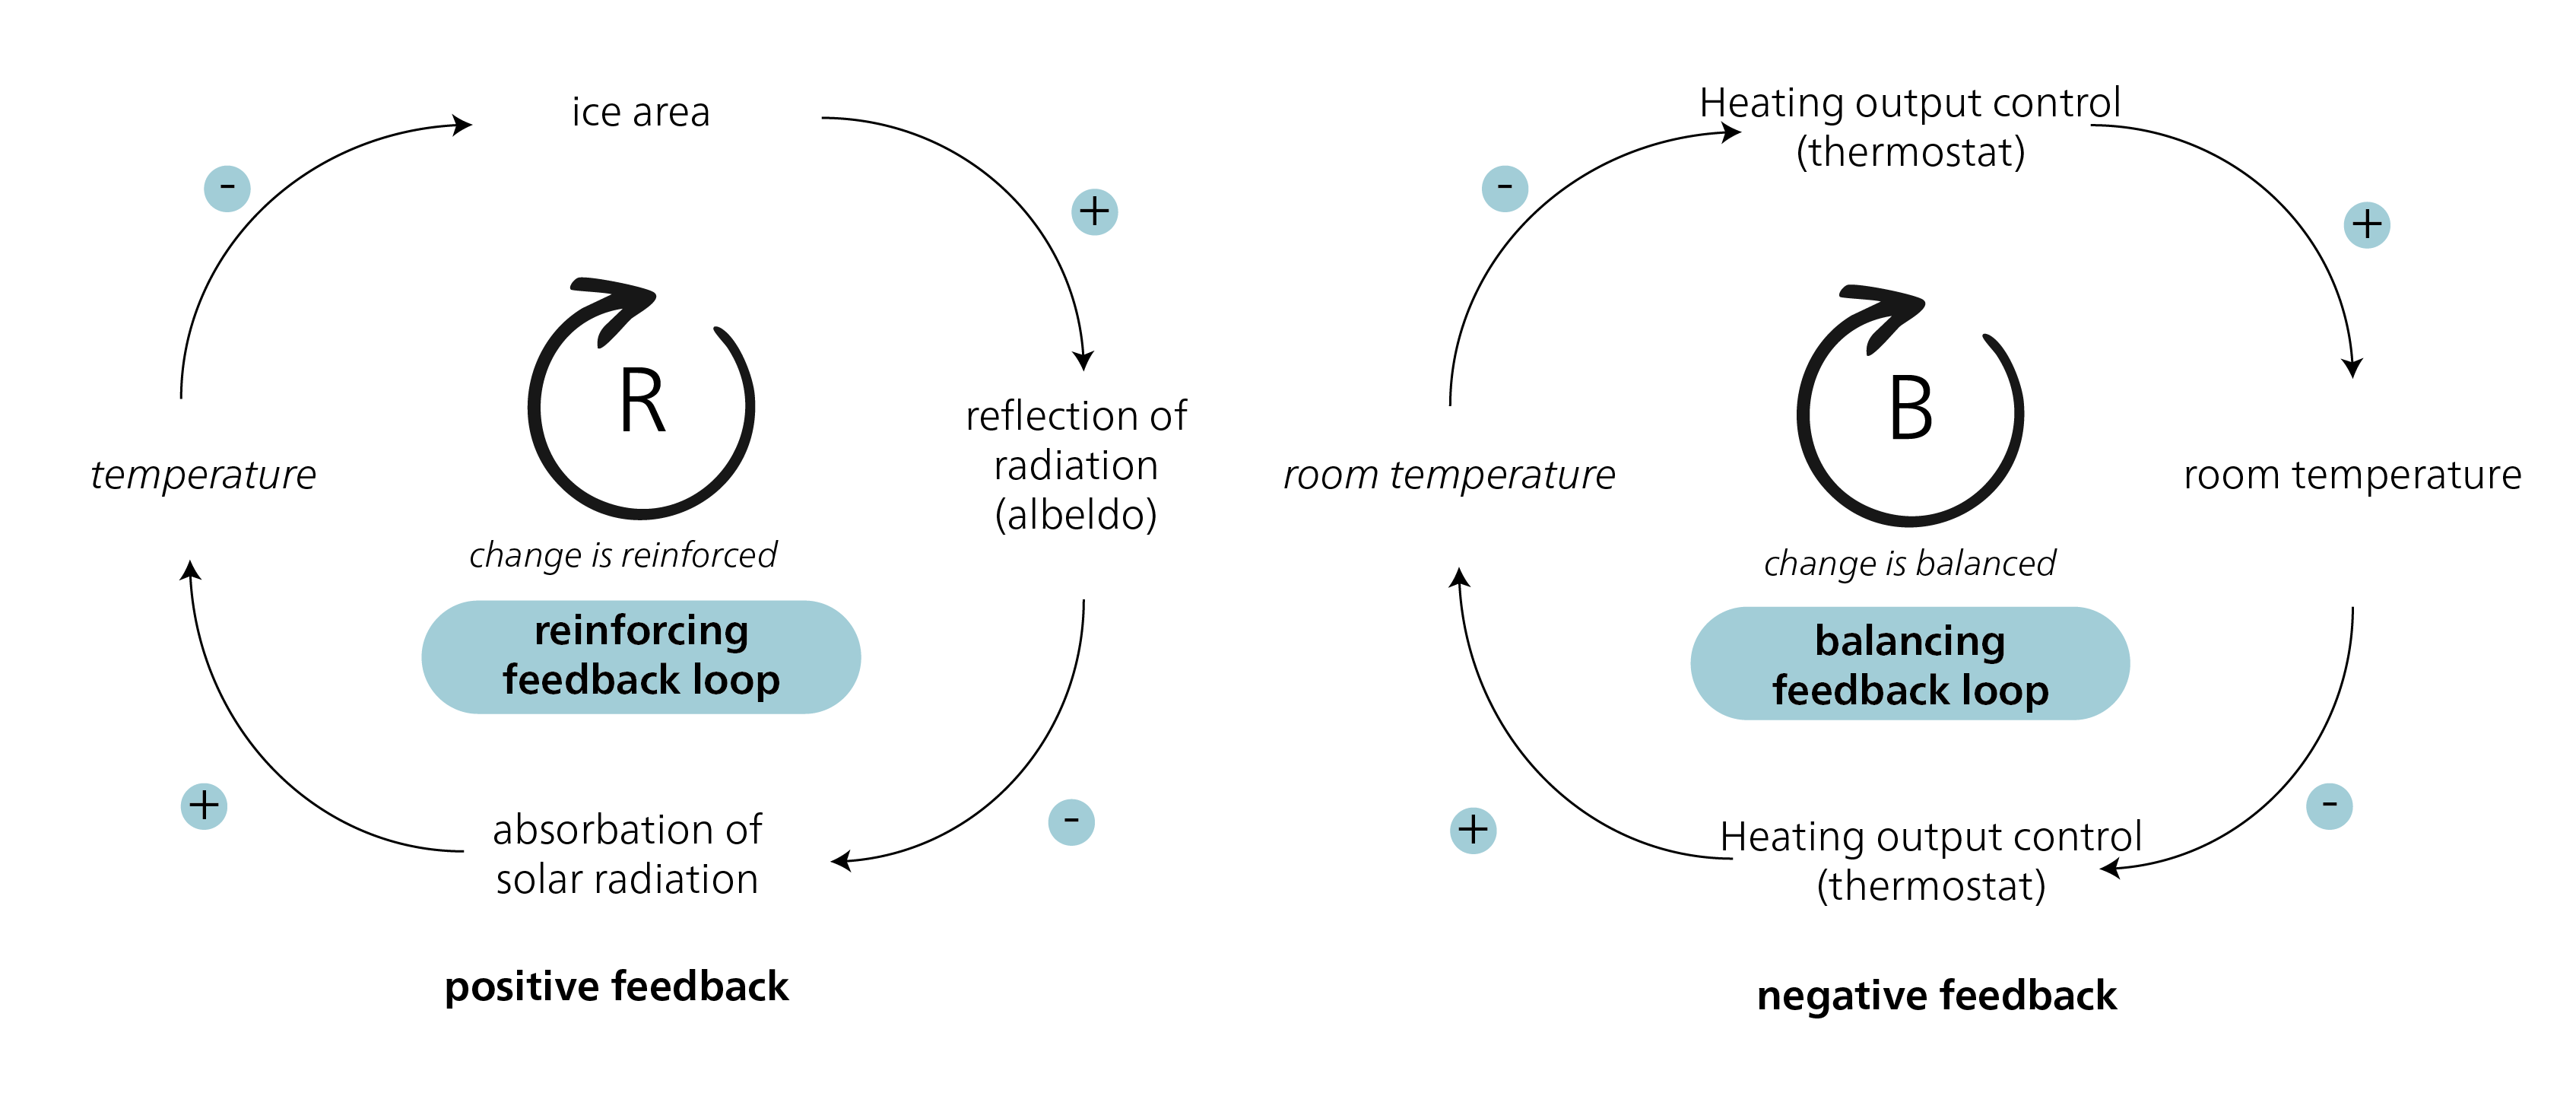
\includegraphics[keepaspectratio]{1_understanding/images/Fig1_15_feedback.png}}

}

\caption{\label{fig-feedback}Positive/verstärkende und
negative/ausgleichende Rückkopplungsschleifen. Quelle: Eigene
Darstellung.}

\end{figure}%

Ein Beispiel für \textbf{positive Rückkopplung} im Zusammenhang mit dem
beschleunigten Schmelzen des arktischen Meereises ist die sogenannte
Albedo-Verstärkung. Das arktische Eis reflektiert einen grossen Teil der
Sonnenstrahlung zurück ins Weltall, wodurch weniger Wärme vom Ozean
aufgenommen wird. Wenn das Eis jedoch schmilzt, wird weniger Sonnenlicht
reflektiert, da das dunklere Meerwasser mehr Wärme absorbiert. Dies
erwärmt das Meerwasser weiter und das verbleibende Eis schmilzt noch
schneller. Dieser Prozess verstärkt sich selbst: Weniger Eis führt zu
einer geringeren Albedo, was wiederum zu einer stärkeren Absorption von
Sonnenlicht und weiterem Schmelzen führt. Diese positive Rückkopplung
hat gravierende Auswirkungen auf das Klimasystem, da das schwindende
arktische Meereis zu einem schnelleren Anstieg des Meeresspiegels und zu
Veränderungen in ozeanischen und atmosphärischen Zirkulationsmustern
führen kann. Das Ausmass und die Geschwindigkeit dieser Entwicklung
überraschten die Wissenschaft (Stroeve u.~a. 2007).

Ein Beispiel für \textbf{negative Rückkopplung} ist ein Thermostat, der
die Temperatur in einem Raum reguliert. Steigt die Raumtemperatur über
den eingestellten Maximalwert, erkennt der Thermostat dies und aktiviert
die Klimaanlage, um die Temperatur zu senken. Sobald die Temperatur den
eingestellten Wert erreicht, schaltet der Thermostat die Klimaanlage ab.
Dieser Regelkreis sorgt dafür, dass die Raumtemperatur auf einem
konstanten Niveau gehalten wird.

Positive und negative Rückkopplungen wirken oft gemeinsam und können
komplexes Verhalten in Systemen hervorrufen. Das Verständnis dieser
Rückkopplungsmechanismen ermöglicht es, die Interaktionen und das
Verhalten von Systemen besser zu analysieren und vorherzusagen.

\section{Nachhaltigkeitswissenschaft: Entstehung und
Verständnis}\label{nachhaltigkeitswissenschaft-entstehung-und-verstuxe4ndnis}

Ein aufkommendes Problembewusstsein -- nicht zuletzt beeinflusst durch
die Veröffentlichung \emph{The Limits to Growth} (Meadows u.~a. 1972) --
führte zu verstärkter Forschung über globale Umweltprobleme. Drei grosse
internationale Forschungsprogramme sind hierbei besonders bemerkenswert:
1) das \emph{International Geosphere-Biosphere Programme} (IGBP) von
1987 bis 2015, 2) das \emph{World Climate Research Programme} (WCRP),
gegründet 1980, und 3) das International Research Programme on
Biodiversity (DIVERSITAS), gegründet 1991 und 2014 in \emph{Future
Earth} umbenannt. Diese Programme haben nicht nur wichtige
Grundlagenforschung initiiert -- sie gaben auch wesentliche Impulse für
eine stärkere Berücksichtigung der Ergebnisse in der Politik, wie sie
sich etwa im Brundtland-Bericht der Vereinten Nationen und in der Agenda
21 widerspiegeln. Besonders hervorzuheben ist, dass diese
Forschungsprogramme erstmals systematisch zuvor getrennte Disziplinen
der Naturwissenschaften zusammenführten, auch wenn die Wechselwirkungen
zwischen Gesellschaft und Umwelt weitgehend unberücksichtigt blieben.
Als das Bewusstsein für die Verflechtung dieser Themen zunahm, wurden
insbesondere in den USA mehrere Forschungsprojekte initiiert, die diese
Integration vorantrieben.

\begin{quote}
„Ein neues Feld der Nachhaltigkeitswissenschaft entsteht, das versucht,
den grundlegenden Charakter der Wechselwirkungen zwischen Natur und
Gesellschaft zu verstehen. Ein solches Verständnis muss das
Zusammenwirken globaler Prozesse mit den ökologischen und sozialen
Besonderheiten bestimmter Orte und Sektoren umfassen.'' (Kates u.~a.
2001, pp.~641)
\end{quote}

Das Konzept der Nachhaltigkeitswissenschaft wurde 2001 auf dem Kongress
„Challenges of a Changing Earth'' in Amsterdam offiziell eingeführt --
durch den International Council for Science (ICSU), das oben genannte
IGBP, das International Human Dimensions Programme on Global
Environmental Change (IHDP) und das oben genannte WCRP. Der
deutschsprachige Begriff „Nachhaltigkeitswissenschaft'' geht auf eine
Übersetzung aus dem Englischen zurück.

\subsection{Verständnis der
Nachhaltigkeitswissenschaft}\label{verstuxe4ndnis-der-nachhaltigkeitswissenschaft}

Ein häufig verwendetes Motto -- „Die Gesellschaft hat Probleme -- die
Universitäten haben Disziplinen'' -- verdeutlicht die konventionelle
Struktur der Wissenschaft in verschiedene Fachrichtungen. Disziplinäre
Wissenschaft scheint jedoch unzureichend gerüstet zu sein, um die
Herausforderungen Nachhaltiger Entwicklung zu bewältigen. Zwei
Hauptansätze zum Verständnis der Nachhaltigkeitswissenschaft haben sich
herausgebildet: Einerseits wird sie als eigenständige Disziplin mit
eigenen Theorien und Methoden betrachtet, andererseits als ein
Zusammenschluss verschiedener Disziplinen, die sich auf ein gemeinsames
Thema konzentrieren (Clark und Dickson 2003). Während der erste Ansatz
noch nicht als zutreffend gilt, besteht weitgehend Einigkeit darüber,
dass die Nachhaltigkeitswissenschaft als Plattform verstanden werden
sollte, auf der Wissenschaft, Praxis und Visionen zusammenkommen -- und
die Beiträge aus dem gesamten Spektrum der Natur-, Wirtschafts- und
Sozialwissenschaften integriert (Martens 2006, pp.~38).

Die Nachhaltigkeitswissenschaft unterscheidet sich in zwei zentralen
Punkten: Erstens ist sie -- im Gegensatz zur traditionellen („Mode 1'')
Forschung -- nicht durch ein originäres wissenschaftliches Programm
getrieben. Stattdessen wird sie durch das normative Konzept der
Nachhaltigkeit geleitet und nutzt dieses als Rahmen für
wissenschaftliche Analysen. Zweitens unterscheidet sie sich als
eigenständiger Typ problemorientierter Forschung sowohl von Grundlagen-
als auch von angewandter Forschung. Clark (2007) prägte hierfür den
Begriff der „anwendungsorientierten Grundlagenforschung'', die darauf
abzielt, neues Wissen zu generieren und gleichzeitig dessen potenzielle
Anwendungen zu berücksichtigen.

\begingroup\fontsize{8}{10}\selectfont

\begin{longtable}[t]{>{\raggedright\arraybackslash}p{4.5cm}>{\raggedright\arraybackslash}p{4.5cm}l}

\caption{\label{tbl-mode1-mode2-science}Mode-1- und Mode-2-Wissenschaft.
Quelle: Basierend auf Gibbons u.~a. (2010) und Martens (2006).}

\tabularnewline

\toprule
\textbf{Dimension} & \textbf{Mode-1-Wissenschaft} & \textbf{Mode-2-Wissenschaft}\\
\midrule
\endfirsthead
\multicolumn{3}{@{}l}{\textit{(continued)}}\\
\toprule
\textbf{Dimension} & \textbf{Mode-1-Wissenschaft} & \textbf{Mode-2-Wissenschaft}\\
\midrule
\endhead

\endfoot
\bottomrule
\endlastfoot
\textbf{Orientierung} & Akademisch & Akademisch und gesellschaftlich\\
\textbf{Disziplinarität} & Monodisziplinär & Trans- und interdisziplinär\\
\textbf{Steuerung} & Technokratisch & Partizipativ\\
\textbf{Wissensstatus} & Gewiss & Unsicher\\
\textbf{Ansatz} & Prädiktiv & Explorativ\\*

\end{longtable}

\endgroup{}

\subsection{Empirisch-analytisch versus
normativ}\label{empirisch-analytisch-versus-normativ}

Da Nachhaltige Entwicklung ein normatives Leitbild ist, ist es wichtig,
zwischen deskriptiver (empirisch-analytischer) und präskriptiver
(normativer) Forschung zu unterscheiden. Deskriptive Aussagen
beschreiben den aktuellen Zustand („Sein''), während normative Aussagen
den idealen Zustand („Sollen'') darstellen. Im Alltag wird diese
Unterscheidung zwischen „Sein'' und „Sollen'' oft nicht wahrgenommen,
doch für die Wissenschaft ist sie von entscheidender Bedeutung.

\begin{figure}[H]

\centering{

\pandocbounded{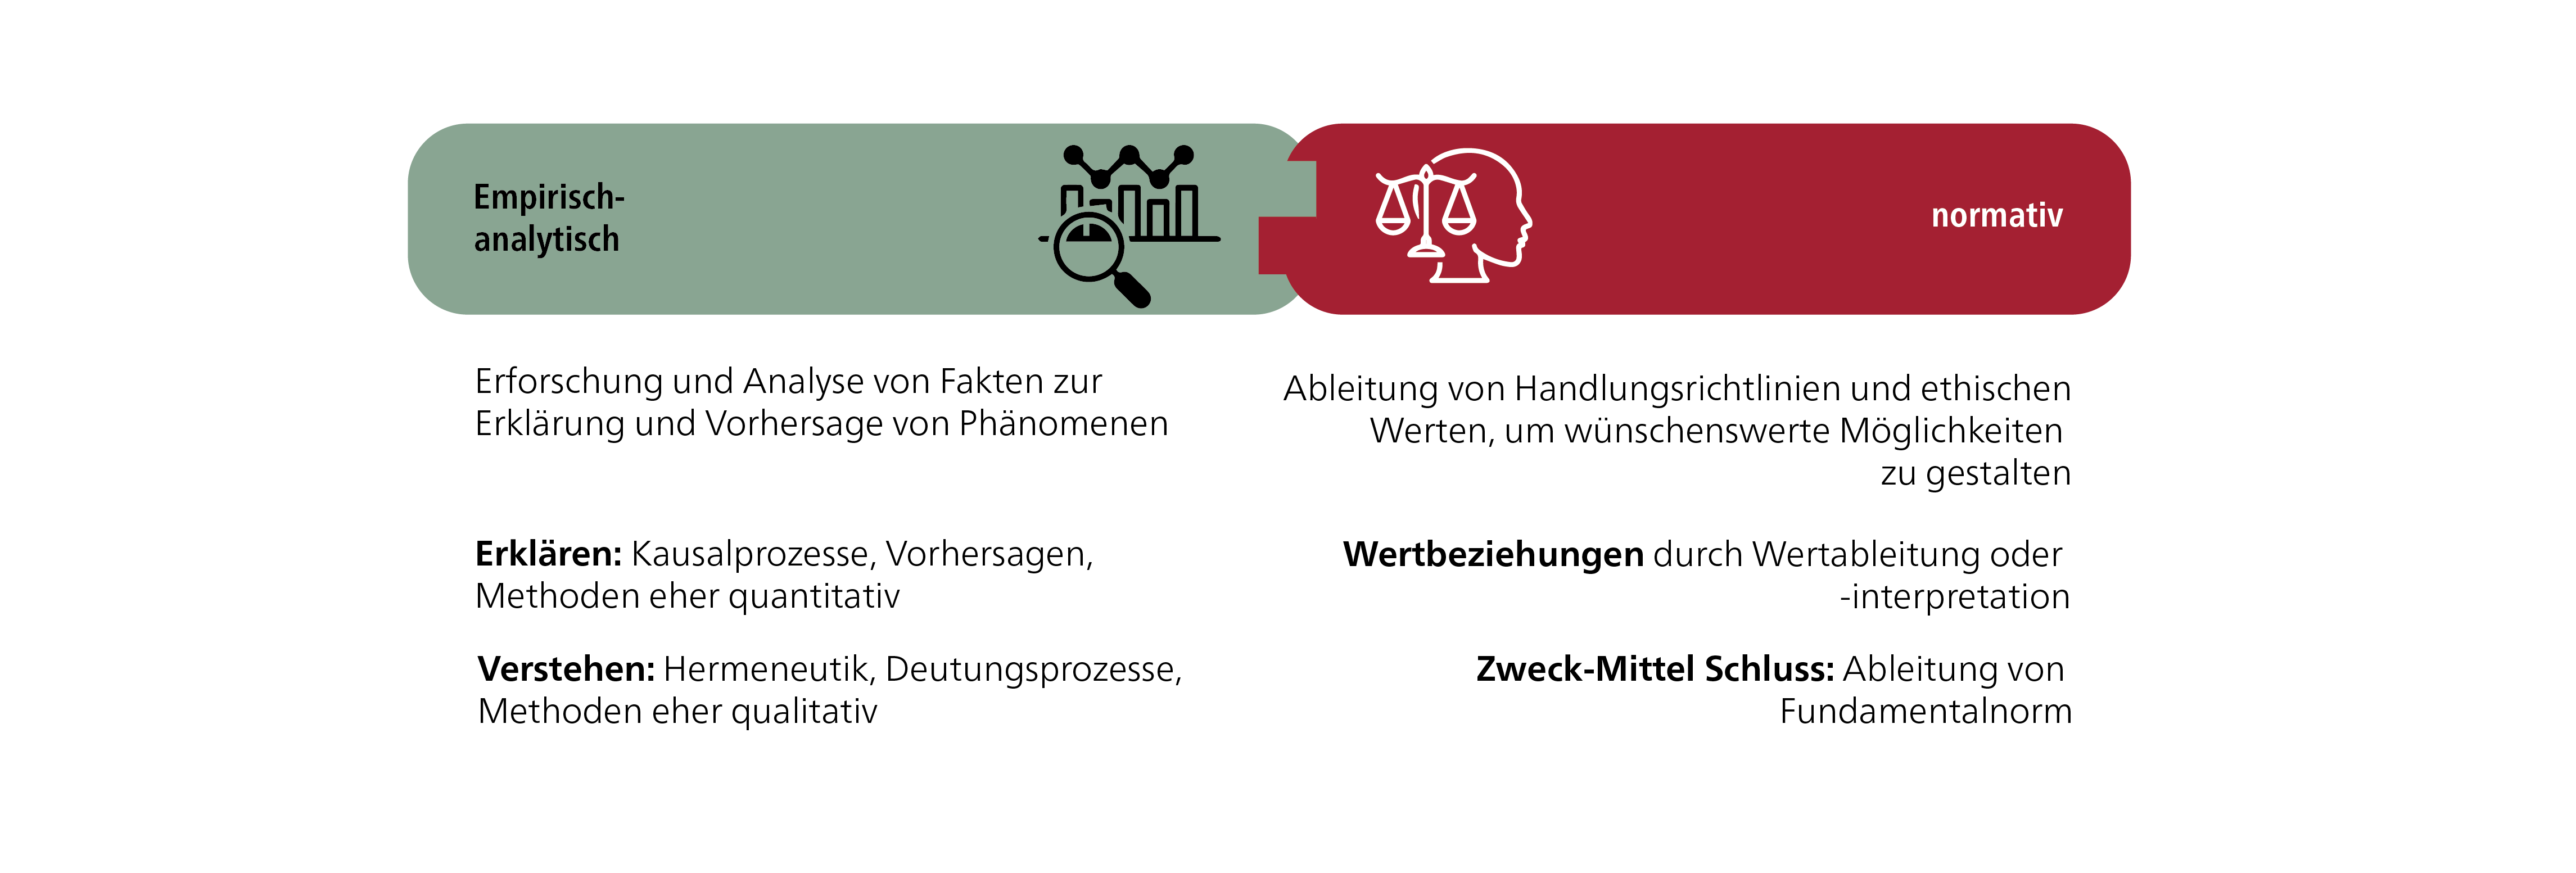
\includegraphics[keepaspectratio]{1_understanding/images/emprical-analytical_normative.png}}

}

\caption{\label{fig-emprical-analytical_normative}Unterscheidung
zwischen empirisch-analytisch und normativ. Quelle: Eigene Darstellung.}

\end{figure}%

Es ist wichtig zu beachten, dass „Sein''- und „Sollen''-Aussagen
unterschiedliche Qualitäten und Gegenstandsbereiche haben und nicht ohne
weitere Erklärung miteinander verknüpft werden können. Dieses
Verständnis bildet die Grundlage von Humes Gesetz, das besagt, dass
normative Aussagen darüber, „was sein soll'', nicht aus deskriptiven
Aussagen darüber, „was ist'', abgeleitet werden können. Ein drastisches
Beispiel: Die Tatsache, dass täglich rund 24.000 Menschen verhungern,
erlaubt keinerlei Schluss darüber, ob dies gut oder schlecht ist. Ohne
eine Bewertung kann keine normative Aussage darüber getroffen werden, ob
dies verhindert werden sollte. Hume wies darauf hin, dass viele
Wissenschaftler*innen seiner Zeit diese entscheidende Unterscheidung
häufig vernachlässigten -- und dies gilt bis heute:

\begin{quote}
„In every system of morality, which I have hitherto met with, I have
always remark'd, that the author proceeds for some time in the ordinary
ways of reasoning, and establishes the being of a God, or makes
observations concerning human affairs; when of a sudden I am surpriz'd
to find, that instead of the usual copulations of propositions, is, and
is not, I meet with no proposition that is not connected with an ought,
or an ought not. This change is imperceptible; but is however, of the
last consequence. For as this ought, or ought not, expresses some new
relation or affirmation, 'tis necessary that it shou'd be observ'd and
explain'd; and at the same time that a reason should be given; for what
seems altogether inconceivable, how this new relation can be a deduction
from others, which are entirely different from it\ldots{} {[}I{]} am
persuaded, that a small attention wou'd subvert all the vulgar systems
of morality, and let us see, that the distinction of vice and virtue is
not founded merely on the relations of objects, nor is perceiv'd by
reason.'' (Hume 1739, Book 3, Part 1, Section 1)
\end{quote}

Die Erkenntnis, dass sich Sein- und Soll-Aussagen unterscheiden,
bedeutet nicht, dass Wissenschaftler*innen keine Soll-Aussagen machen
dürfen. Vielmehr bedeutet sie, dass aufgrund der epistemologischen
Unterschiede zwischen den beiden Kategorien bestimmte Regeln gelten
müssen, wenn sie miteinander verknüpft werden. Hume versuchte, die
Beziehung zwischen diesen beiden Aussagearten durch sogenannte
„Brückenprinzipien'' herzustellen. Max Weber formalisierte diese
Überlegungen weiter, indem er die Brückenprinzipien durch das Konzept
der „Wertbeziehungen'' ersetzte. Webers Forderung nach Wertfreiheit
(bzw. Wertneutralität) in der empirischen Wissenschaft ergibt sich aus
seiner Beobachtung, dass es eine klare Unterscheidung zwischen
Tatsachenfragen („Sein'') und Wertfragen („Sollen'') gibt (Weber 1999,
pp.~245f, 509f). Er argumentierte, dass es nicht Aufgabe der empirischen
Wissenschaften sei, Werturteile zu fällen. Wenn Wissenschaftler*innen
die analytische Trennung zwischen ihren persönlichen Werten und ihren
Forschungszielen nicht vollziehen, könne dies die Fähigkeit der
Wissenschaft gefährden, überprüfbare und sinnvolle Ergebnisse zu
erzeugen (Weber 1999, pp.~150f). Dies könnte wiederum zu einer
Verwischung der Grenzen zwischen wissenschaftlichem Wissen und Wissen
aus Politik, Religion oder Alltagsdiskussionen führen.

Webers Forderung nach Wertfreiheit in der empirischen Wissenschaft wurde
häufig missverstanden (Weber 1999, pp.~499f). Sie bedeutet nicht, dass
Forschung ohne Werte auskommen sollte. (Ausserwissenschaftliche) Werte
haben in der empirischen Forschung -- insbesondere im Kontext
Nachhaltiger Entwicklung -- auf verschiedene Weise ihren Platz:

\begin{itemize}
\item
  \textbf{Werte können Forschungsgegenstand sein:} Werte spielen
  beispielsweise im Bereich der Umwelt- und Nachhaltigkeitspsychologie
  eine zentrale Rolle. In Diskussionen über Lebensstile und subjektives
  Wohlbefinden untersuchen Forschende die persönlichen Werte und
  Überzeugungen von Individuen.
\item
  \textbf{Werte beeinflussen die Wahl des Forschungsthemas:} Werte
  wirken sich auf die Auswahl von Forschungsgegenständen und
  Fragestellungen (Erkenntnisinteresse) und damit auf die Ausrichtung
  der Forschung aus. Dies ist besonders relevant in
  anwendungsorientierter und transdisziplinärer Forschung, in der die
  Bedürfnisse und Informationen relevanter gesellschaftlicher
  Akteur*innen in den Forschungsprozess integriert werden,
  beispielsweise durch \emph{joint problem framing} oder
  \emph{participatory vision development} (Schneider u.~a. 2019).
\item
  \textbf{Wertinterpretationen sollten klar benannt werden:} Forschende
  können Wertbeziehungen herstellen oder Wertinterpretationen vornehmen
  (vgl. Weber 1999, pp.~522). Eine Wertinterpretation, angelehnt an die
  hermeneutische Methode, konkretisiert die Bedeutung übergeordneter
  Wertvorstellungen und leitet daraus logische Werte und Normen ab.
  Beispielsweise können Forschende die SDGs analysieren, indem sie die
  den Zielen Nachhaltiger Entwicklung zugrunde liegenden Werte
  untersuchen. Weitere Beispiele sind Normen, die aus dem
  Gerechtigkeitsbegriff abgeleitet werden -- wie etwa die Norm der
  menschlichen Verantwortung gegenüber der Umwelt, der sozialen Mitwelt
  und uns selbst (vgl. Michelsen und Adomßent 2014, pp.~25; Schneider
  u.~a. 2019). Wichtig ist, den ursprünglichen Wert explizit zu machen.
\item
  \textbf{Zweck-Mittel-Schlüsse:} Die Forschung zur Nachhaltigen
  Entwicklung stützt sich häufig auf Werturteile, um evidenzbasierte
  Lösungen zu entwickeln. Dies ist vergleichbar mit der
  Politikwissenschaft, in der normative Theorien darauf abzielen, eine
  optimale -- d.~h. gerechte -- Staatsform zu entwerfen, basierend auf
  der positiven Bewertung dessen, was eine gerechte Gesellschaft
  ausmacht. Die Wissenschaft kann den Wert von Gerechtigkeit nicht
  beweisen, aber sie kann Strategien und Mittel entwickeln, um dieses
  gewünschte Ziel zu erreichen. Diese Beziehung zwischen Zweck und
  Mitteln stellt eine logische Verbindung zwischen Werten und normativen
  Aussagen dar. Der übergeordnete Zweck wird durch
  ausserwissenschaftliche Werte bestimmt. Forschende müssen diese
  Beziehung klar benennen und ihre Mittel entsprechend formulieren. Ein
  solcher Zweck-Mittel-Zusammenhang könnte etwa so aussehen: „Um Ziel X
  zu erreichen, ist Y unter den Bedingungen b1, b2 und b3 das
  erfolgreichste Mittel.'' Nachhaltige Entwicklung kann als eine
  ausserwissenschaftlich gegebene Fundamentalnorm betrachtet werden.
  Wenn die Forschung beispielsweise Aussagen darüber treffen will, wie
  Nachhaltige Entwicklung durch Solarenergie erreicht werden kann,
  könnte sie folgendermassen vorgehen: „Die Umstellung auf eine solare
  Produktionsweise könnte ein vielversprechender Weg sein, Nachhaltige
  Entwicklung zu erreichen. Dies würde Produktion und Verteilung
  entsprechend den Bedürfnissen vieler Menschen organisieren, soziale
  Ungleichheiten minimieren und Bedingungen für individuelles
  Wohlbefinden schaffen.''
\end{itemize}

\section{Wissensarten für die Nachhaltige
Entwicklung}\label{wissensarten-fuxfcr-die-nachhaltige-entwicklung}

Die Nachhaltigkeitsforschung befasst sich mit Herausforderungen, die die
langfristige Sicherung der gesellschaftlichen Entwicklungsbedingungen
bedrohen. Im Kontext der Nachhaltigen Entwicklung als
gesamtgesellschaftlicher Aufgabe beschreibt das Forum für Klima und
Globalen Wandel der Akademie der Naturwissenschaften Schweiz drei
verschiedene Wissensarten (ProClim 1997): System-, Ziel- und
Transformationswissen. Diese drei Wissensarten lassen sich drei
grundlegenden Ebenen zuordnen: 1) der analytischen Ebene, die auf die
Generierung von Systemwissen abzielt, 2) der normativen Ebene, die Ziel-
und Orientierungswissen entwickelt, und 3) der operativen Ebene, die auf
die Erzeugung von Gestaltungs- bzw. Transformationswissen ausgerichtet
ist. Abbildung~\ref{fig-Three-Knowledge-Types} zeigt die drei
Wissensarten in Relation zu empirisch-analytischer und normativer
Forschung.

\begin{figure}[H]

\centering{

\pandocbounded{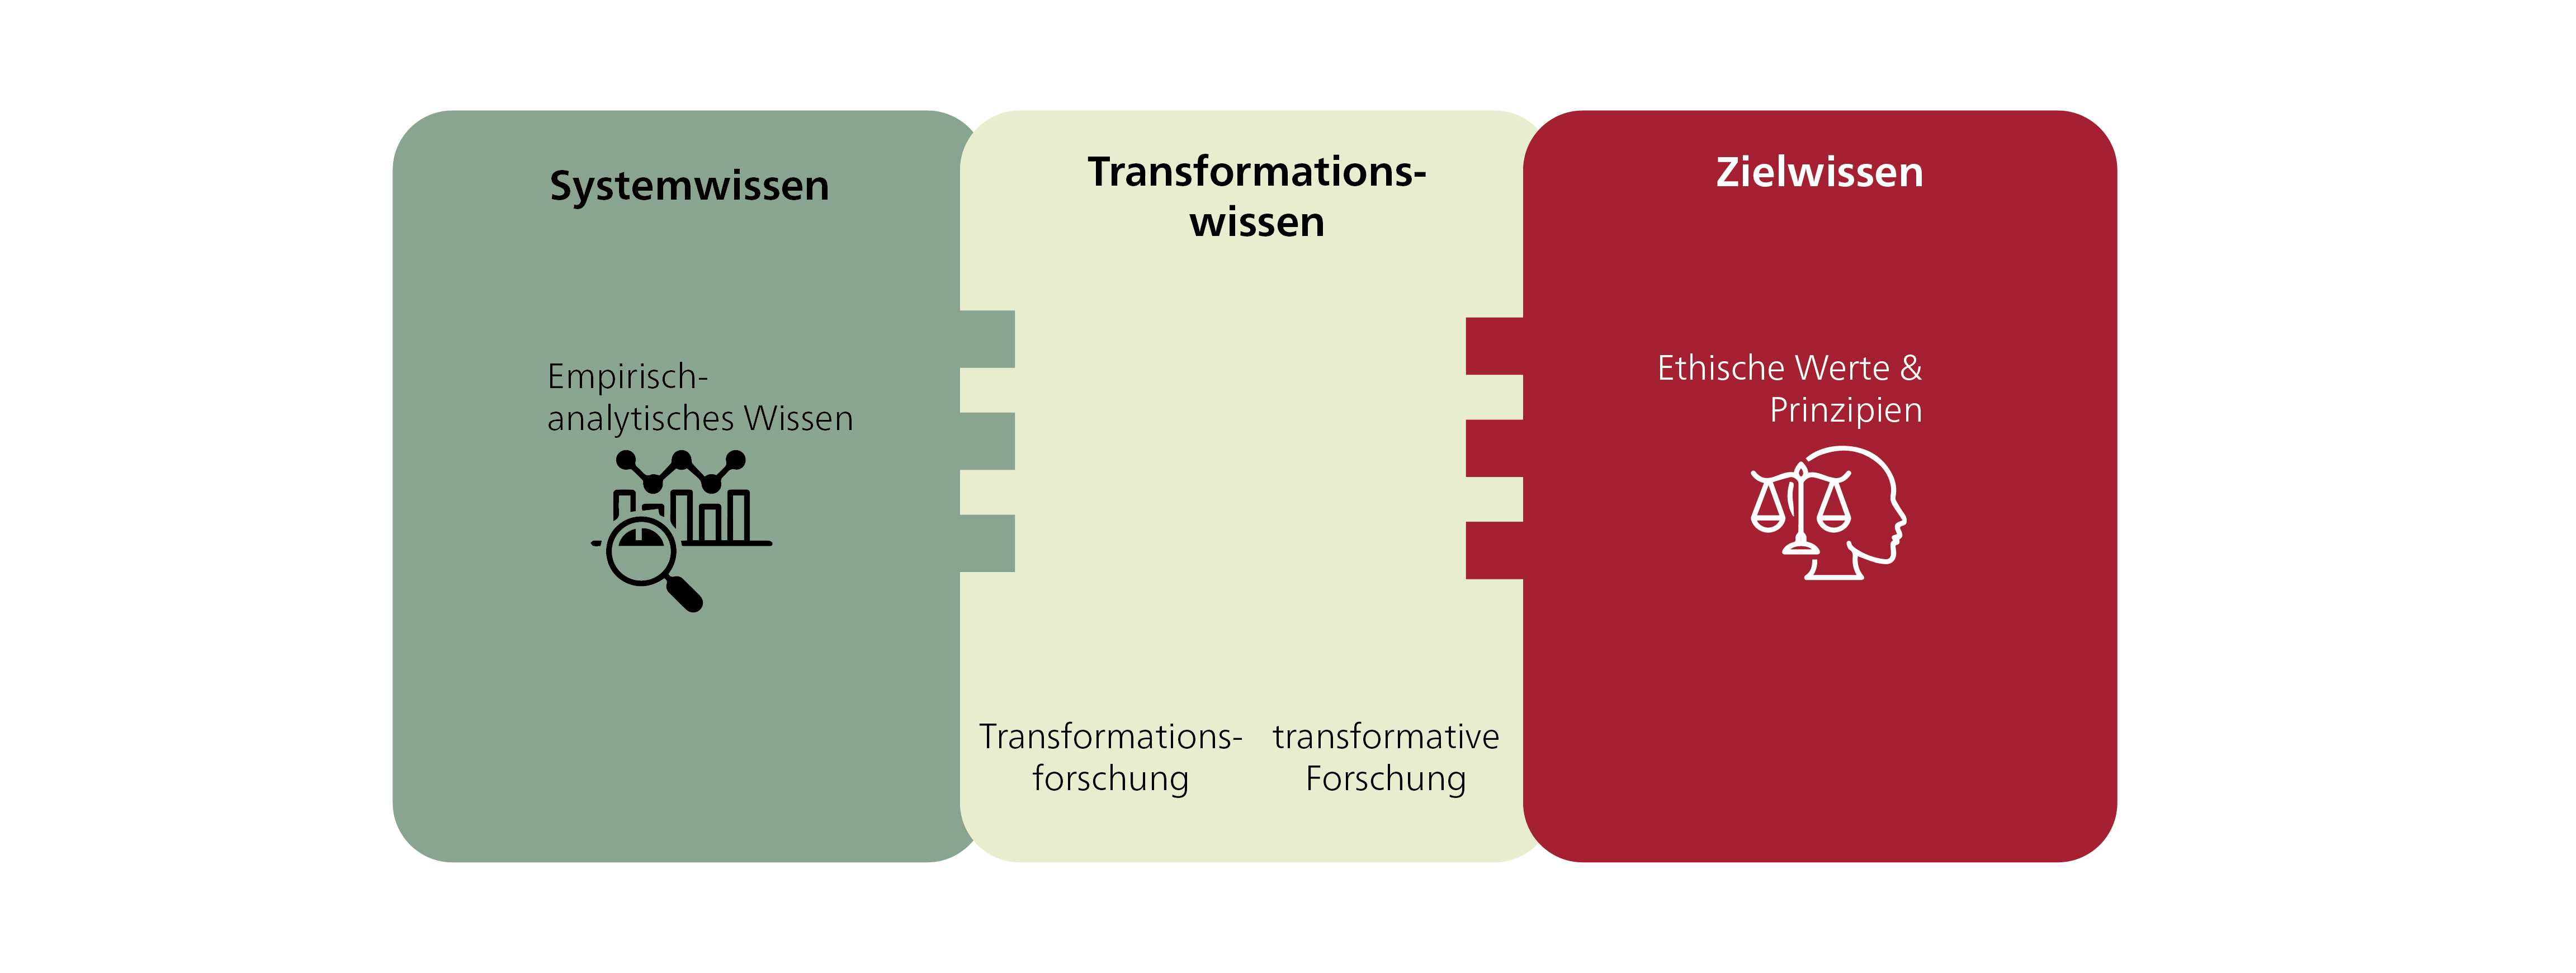
\includegraphics[keepaspectratio]{1_understanding/images/Three-Knowledge-Types.png}}

}

\caption{\label{fig-Three-Knowledge-Types}Die drei Wissensarten. Quelle:
Eigene Darstellung basierend auf ProClim (1997).}

\end{figure}%

\textbf{Systemwissen} bezieht sich auf das Verständnis des aktuellen
Zustands. Im Kontext Nachhaltiger Entwicklung untersucht die Forschung
relevante Strukturen und Prozesse, beschreibt und erklärt deren
Komplexität und Dynamik. Dabei kommen verschiedene Methoden zum Einsatz,
darunter qualitative und quantitative Ansätze, Mixed-Methods-Verfahren,
Experimente und systemdynamische Ansätze. Ebenso werden Prognosen,
Rückblicke und Szenarioanalysen genutzt. Die meisten Studien, die
Systemwissen erzeugen, fallen in den Bereich der empirischen Forschung.

\textbf{Transformationswissen} ist das Wissen darüber, wie wir vom
aktuellen Zustand („Sein'') zum gewünschten Zustand („Sollen'') gelangen
können. Dies erfordert eine Integration von System- und Zielwissen. Mit
anderen Worten: Die Forschung sucht nach nachweislich wirksamen Lösungen
für die im Kontext Nachhaltiger Entwicklung identifizierten Probleme. Es
gibt viele Methoden, um Transformationswissen zu generieren.

Forschung über Transformationen, also über Veränderungen in der
gesellschaftlichen Organisation auf verschiedenen Ebenen, kann sowohl
empirisch als auch normativ sein. Forschung, die sich mit vergangenen
und gegenwärtigen Transformationen befasst, ist empirisch, während
Forschung, die auf konkrete Ziele abzielt, normativ ist. Entsprechend
unterscheidet der Wissenschaftliche Beirat der Bundesregierung Globale
Umweltveränderungen (WBGU) zwischen „Transformationsforschung'' und
„transformativer Forschung''.

Ein weiteres im Kontext von Transformationen betontes Konzept ist die
„transformative Bildung'', die darauf abzielt, Fähigkeiten für ein
umfassendes und vielschichtiges Verständnis von Veränderungsprozessen zu
fördern (Schneidewind 2013). Ziel transformativer Bildung ist es, die
Reflexionsfähigkeit der Gesellschaft zu stärken -- sowohl in Bezug auf
die Beobachtung als auch auf die aktive Mitgestaltung von
Transformationsprozessen.

\textbf{Zielwissen} bezieht sich auf das Wissen darüber, was erreicht
und was vermieden werden sollte. Normative Forschung ist in diesem
Zusammenhang von besonderer Bedeutung. Es geht darum, die Werte
Nachhaltiger Entwicklung zu interpretieren und zu konkretisieren sowie
weitere Normen daraus abzuleiten. Ebenso relevant ist die Forschung zur
Festlegung von Schwellenwerten wie auch die Entwicklung von Methoden für
Bewertungen und Visionierungsprozesse (vgl. Swart u.~a. 2004; Wiek und
Iwaniec 2014). Zielwissen gibt uns die Antwort auf die Frage, was wir
transformieren sollten. Die Studienprogramme des CDE orientieren sich
dabei vor allem an folgenden Konzeptionen von Zielwissen für ein
nachhaltiges Wirtschafts- und Gesellschaftssystem:

\begin{itemize}
\tightlist
\item
  Die Prinzipien Nachhaltiger Entwicklung
\item
  Die Agenda 2030 und die SDGs (2015)
\item
  Das WBGU-Hauptgutachten \emph{Welt im Wandel: Gesellschaftsvertrag für
  eine Grosse Transformation} (2011)
\item
  Der Global Sustainable Development Report GSDR (2019)
\end{itemize}

\section{Grundlagen der Nachhaltigkeit: Das Quiz -- Kapitel
1}\label{grundlagen-der-nachhaltigkeit-das-quiz-kapitel-1}

Welche Aussage definiert „Nachhaltige Entwicklung'' gemäss dem
Brundtland-Bericht am treffendsten?

\begin{itemize}
\tightlist
\item[$\square$]
  Die Verbesserung des Lebensstandards durch Industrialisierung
\item[$\square$]
  Wirtschaftswachstum ohne Umweltschäden
\item[$\square$]
  Entwicklung, die die Bedürfnisse der Gegenwart befriedigt, ohne die
  Fähigkeit künftiger Generationen zu gefährden, ihre eigenen
  Bedürfnisse zu befriedigen
\item[$\square$]
  Die Senkung der CO₂-Emissionen um 50\% bis 2030
\end{itemize}

Der Brundtland-Bericht (1987) definiert Nachhaltige Entwicklung als eine
Entwicklung, die die Bedürfnisse der Gegenwart befriedigt, ohne die
Fähigkeit künftiger Generationen zu gefährden, ihre eigenen Bedürfnisse
zu befriedigen.

\begin{itemize}
\tightlist
\item
  False
\item
  False
\item
  True
\item
  False
\end{itemize}

Was ist Normativität?

\begin{itemize}
\tightlist
\item[$\square$]
  Bezieht sich auf Werte und moralisch begründete Vorstellungen davon,
  was getan werden sollte und wie die Dinge sein sollten
\item[$\square$]
  Bedeutet, dass Handlungen auf gemeinsam vereinbarten Gesetzen und
  Normen beruhen sollten
\item[$\square$]
  Bezieht sich darauf, wie die Dinge gegenwärtig sind
\end{itemize}

Normativität bezieht sich auf Werte, Normen und moralisch begründete
Vorstellungen davon, was getan werden sollte und wie die Dinge sein
sollten, anstatt zu beschreiben, wie die Dinge gegenwärtig sind.

\begin{itemize}
\tightlist
\item
  True
\item
  False
\item
  False
\end{itemize}

Was ist die „Grosse Beschleunigung''?

\begin{itemize}
\tightlist
\item[$\square$]
  Der plötzliche Rückgang der Biodiversität zu Beginn des 21.
  Jahrhunderts
\item[$\square$]
  Das exponentielle Wachstum sozioökonomischer und Erdsystem-Trends, das
  Mitte des 20. Jahrhunderts einsetzte
\item[$\square$]
  Ein rascher Anstieg des globalen Ressourcenverbrauchs nach dem Ersten
  Weltkrieg
\item[$\square$]
  Der rasche Rückgang der Industrialisierung in den 1960er-Jahren
\end{itemize}

Die „Grosse Beschleunigung'' bezeichnet den raschen und exponentiellen
Anstieg sozioökonomischer Aktivitäten (wie Bevölkerungswachstum,
Industrialisierung und Ressourcenverbrauch) sowie die entsprechenden
Veränderungen der Erdsystemprozesse, die etwa Mitte des 20. Jahrhunderts
einsetzten.

\begin{itemize}
\tightlist
\item
  False
\item
  True
\item
  False
\item
  False
\end{itemize}

Was unterscheidet „starke'' von „schwacher'' Nachhaltigkeit?

\begin{itemize}
\tightlist
\item[$\square$]
  Beide Konzepte bedeuten dasselbe.
\item[$\square$]
  Starke Nachhaltigkeit erlaubt die vollständige Substitution von
  Naturkapital.
\item[$\square$]
  Starke Nachhaltigkeit verlangt, Naturkapital als nicht substituierbar
  zu erhalten.
\item[$\square$]
  Schwache Nachhaltigkeit schränkt jegliche technologische Innovation
  ein.
\end{itemize}

Starke Nachhaltigkeit geht davon aus, dass bestimmte ökologische
Funktionen und Naturkapitalbestände kritisch sind und nicht durch von
Menschen geschaffenes oder technologisches Kapital ersetzt werden
können, während schwache Nachhaltigkeit eine solche Substitution
zulässt.

\begin{itemize}
\tightlist
\item
  False
\item
  False
\item
  True
\item
  False
\end{itemize}

Welche Aussagen beschreiben den Unterschied zwischen starker und
schwacher Nachhaltigkeit korrekt? (Mehr als eine Aussage kann richtig
sein.)

\begin{itemize}
\tightlist
\item[$\square$]
  Bei schwacher Nachhaltigkeit können sich verschiedene Kapitalformen
  gegenseitig ersetzen.
\item[$\square$]
  Schwache Nachhaltigkeit geht davon aus, dass technologische Innovation
  die Funktionen der Natur vollständig ersetzen kann.
\item[$\square$]
  Starke Nachhaltigkeit akzeptiert eine unbegrenzte Substitution
  zwischen Natur- und von Menschen geschaffenem Kapital.
\item[$\square$]
  Bei starker Nachhaltigkeit gilt Naturkapital als nicht substituierbar.
\end{itemize}

Schwache Nachhaltigkeit beruht auf der Annahme, dass sich verschiedene
Kapitalformen (Natur-, Sach- und Sozialkapital) gegenseitig ersetzen
können und dass technologischer Fortschritt den Verlust von Naturkapital
kompensieren kann. Starke Nachhaltigkeit hingegen geht davon aus, dass
Naturkapital unverzichtbar ist und nicht ersetzt werden kann, ohne
irreversible Schäden zu riskieren.

\begin{itemize}
\tightlist
\item
  True
\item
  True
\item
  False
\item
  True
\end{itemize}

Welche der folgenden Aussagen beschreiben schwache Nachhaltigkeit? (Mehr
als eine Aussage kann richtig sein.)

\begin{itemize}
\tightlist
\item[$\square$]
  Die Erhaltung von Naturkapital, wenn dies das menschliche Wohlergehen
  fördert oder bewahrt.
\item[$\square$]
  Die Bedürfnisse der gegenwärtigen Generation werden gegenüber jenen
  künftiger Generationen bevorzugt.
\item[$\square$]
  Steigendes BIP.
\item[$\square$]
  Kapitalformen sind grundsätzlich gegenseitig austauschbar.
\item[$\square$]
  Unzureichender Umweltschutz.
\item[$\square$]
  Die Erhaltung der Gesamtsumme aller Kapitalformen von einer Generation
  zur nächsten.
\item[$\square$]
  Ein Unternehmen erfüllt nur seine gesetzlichen Umwelt- und
  Sozialpflichten.
\item[$\square$]
  Die Unersetzbarkeit von durch Menschen geschaffenem Kapital.
\end{itemize}

Schwache Nachhaltigkeit konzentriert sich darauf, den Gesamtbestand an
Kapital über Generationen hinweg zu erhalten, unter der Annahme, dass
sich verschiedene Kapitalformen gegenseitig ersetzen können.
Naturkapital wird vor allem insoweit erhalten, als es zum menschlichen
Wohlergehen beiträgt, statt als grundsätzlich unersetzbar zu gelten.

\begin{itemize}
\tightlist
\item
  True
\item
  False
\item
  False
\item
  True
\item
  False
\item
  True
\item
  False
\item
  False
\end{itemize}

Welche der folgenden Aussagen beschreiben starke Nachhaltigkeit? (Mehr
als eine Aussage kann richtig sein.)

\begin{itemize}
\tightlist
\item[$\square$]
  Das sechste Massenaussterben gilt als das wichtigste
  Nachhaltigkeitsproblem.
\item[$\square$]
  Umweltprobleme werden durch innovative Energietechnologien gelöst.
\item[$\square$]
  Die Natur wird als eine Form von Kapital betrachtet, die auf
  unschätzbare Weise zum Wohlergehen der Menschen beiträgt.
\item[$\square$]
  Eine Zunahme der Gesamtsumme aller Kapitalformen wird gefordert.
\item[$\square$]
  Naturkapital und von Menschen geschaffenes Kapital ergänzen sich, und
  Menschen können ohne beide nicht überleben.
\item[$\square$]
  Die Erhaltung kritischen Naturkapitals von einer Generation zur
  nächsten ist erforderlich.
\end{itemize}

Starke Nachhaltigkeit betont die wesentliche und nicht substituierbare
Rolle des Naturkapitals für das Überleben und Wohlergehen des Menschen.
Sie verlangt die Erhaltung kritischen Naturkapitals über Generationen
hinweg und erkennt an, dass die Natur unverzichtbare Beiträge zum
menschlichen Wohlergehen leistet, die nicht vollständig durch von
Menschen geschaffenes Kapital oder technologische Innovation ersetzt
werden können.

\begin{itemize}
\tightlist
\item
  False
\item
  False
\item
  True
\item
  False
\item
  True
\item
  True
\end{itemize}

Was ist das primäre Ziel der Konsistenzstrategie in der Nachhaltigkeit?

\begin{itemize}
\tightlist
\item[$\square$]
  Bedürfnisse der Konsument*innen mit ökologisch verträglichen Methoden
  erfüllen
\item[$\square$]
  Den Energieverbrauch in der Produktion senken
\item[$\square$]
  Soziale Ungleichheit verringern
\item[$\square$]
  Den Rohstoffeinsatz in der Produktion minimieren
\end{itemize}

Die Konsistenzstrategie zielt darauf ab, wirtschaftliche Aktivitäten und
Konsummuster mit natürlichen Systemen in Einklang zu bringen, indem
Produkte, Prozesse und Dienstleistungen so gestaltet werden, dass sie
ökologisch verträglich sind und gleichzeitig menschliche Bedürfnisse
erfüllen.

\begin{itemize}
\tightlist
\item
  True
\item
  False
\item
  False
\item
  False
\end{itemize}

Welche der folgenden Aussagen zu Nachhaltigkeitsstrategien sind korrekt?
(Mehr als eine Aussage kann richtig sein.)

\begin{itemize}
\tightlist
\item[$\square$]
  Suffizienz fördert höhere Produktionsmengen.
\item[$\square$]
  Effizienz zielt darauf ab, weniger Ressourcen pro Produktionseinheit
  einzusetzen.
\item[$\square$]
  Alle drei Nachhaltigkeitsstrategien wirken sich gleich auf den Konsum
  aus.
\item[$\square$]
  Konsistenz bedeutet, Güter herzustellen, die unendlich oft recycelt
  werden können.
\end{itemize}

Effizienz konzentriert sich auf die Senkung des Ressourceneinsatzes pro
Produktionseinheit. Konsistenz zielt darauf ab, die Produktion an
natürliche Kreisläufe anzupassen, etwa durch geschlossene oder unendlich
recycelbare Systeme. Suffizienz stellt das Ausmass von Produktion und
Konsum infrage, weshalb sich die drei Strategien in ihrer Wirkung auf
den Konsum unterscheiden.

\begin{itemize}
\tightlist
\item
  False
\item
  True
\item
  False
\item
  True
\end{itemize}

\part{Ansätze zur Nachhaltigen Entwicklung}

\chapter{Ansätze zur Nachhaltigen
Entwicklung}\label{ansuxe4tze-zur-nachhaltigen-entwicklung-1}

Die Welt steht vor zahlreichen Herausforderungen der Nachhaltigen
Entwicklung, darunter drängende Umweltprobleme und soziale
Ungleichheiten. Wissenschaftler*innen, Forscher*innen und Aktivist*innen
suchen nach innovativen Ansätzen, um einen nachhaltigen und gerechten
Wandel zu ermöglichen. Dieses Kapitel beleuchtet einige dieser Ansätze,
die ein vollständiges Umdenken bestehender Paradigmen fordern.

Im Kapitel behandelte Ansätze:

\begin{itemize}
\item
  Konzept der planetaren Grenzen
\item
  Doughnut-Ökonomie
\item
  Ansätze zur „Grossen Transformation''
\item
  Grüne Wirtschaft
\item
  Postwachstumsansätze
\item
  Umsetzung der Agenda 2030
\end{itemize}

\section{Debatten über planetare
Grenzen}\label{debatten-uxfcber-planetare-grenzen}

Im Jahr 1798 veröffentlichte der britische Ökonom Thomas Robert Malthus
seinen einflussreichen Essay \emph{An Essay on the Principle of
Population}. Malthus' Kernidee war, dass das Bevölkerungswachstum die
Fähigkeit der Erde, Nahrung zu produzieren, übersteigen würde -- eine
Debatte über die Tragfähigkeit des Planeten, die bis heute anhält.
\emph{The Limits to Growth} (1972), ein Bericht des Club of Rome, baute
auf Malthus' Ideen auf. Er ging über die blosse Nahrungsversorgung
hinaus und berücksichtigte bei der Berechnung einer planetaren Grenze
ein breiteres Spektrum an Faktoren, darunter Ressourcenverfügbarkeit,
Umweltverschmutzung und Industrieproduktion. Der Bericht bleibt aus
ökologischer Sicht relevant, da er die Annahmen eines grenzenlosen
Wachstums in Frage stellt, auch wenn seine spezifischen Prognosen nicht
ganz eingetroffen sind.

Eine bedeutende Entwicklung in der Nachhaltigkeitswissenschaft ist das
Konzept der planetaren Grenzen, das 2009 eingeführt wurde. Im Gegensatz
zu früheren Theorien, die sich ausschliesslich auf Bevölkerungsgrenzen
konzentrierten, verwendet dieses Konzept Parameter der
Erdsystemwissenschaft. Die Forscher*innen identifizierten das Holozän
als Ausgangspunkt, da es eine Periode bemerkenswerter Stabilität für die
menschliche Entwicklung war. Erhebliche Abweichungen von diesem idealen
Zustand könnten die Menschheit auf ungewisse „Kipppunkte'' zutreiben --
kritische Schwellen, die entweder den bisherigen Fortschritt
unterbrechen, seinen Verlauf verändern oder ihn sogar in unbeabsichtigte
Richtungen beschleunigen könnten. Ein Beispiel könnte das Aussterben der
Megafauna am Ende der letzten Eiszeit sein, das möglicherweise mit der
Ankunft des Menschen in Amerika zusammenhing. Das Konzept der planetaren
Grenzen fördert das Vorsorgeprinzip und mahnt zur Handlung, um
potenzielle Schäden für Menschen und Umwelt zu minimieren.

Das Konzept, das neun planetare Grenzen benennt, wurde erstmals von
Rockström et al. (2009) vorgestellt. Es wurde von Steffen et al. (2015)
aktualisiert. Eine aktuelle Aktualisierung von Richardson u.~a. (2023)
zeigt, dass sechs von neun planetaren Grenzen bereits überschritten
wurden.

Das Rahmenwerk der planetaren Grenzen identifiziert neun kritische
Erdsystemprozesse. Diese Prozesse regulieren die Stabilität des Planeten
und umfassen beispielsweise Landnutzungsveränderungen und
Ozeanversauerung (alle planetaren Grenzen sind hier dargestellt:
Abbildung~\ref{fig-development-planetary-boundaries}). Jede Grenze hat
einen inneren Kreis, innerhalb dessen sie sicher betrieben werden kann
(„sicherer Handlungsraum''), und einen äusseren Kreis, der erhöhte
Unsicherheit darstellt.

Die jüngste Aktualisierung des Rahmenwerks der planetaren Grenzen
zeichnet ein besorgniserregendes Bild. Die sichere Grenze für die
Ozeanversauerung droht überschritten zu werden, und die regionale
atmosphärische Aerosolbelastung hat ihre Grenze bereits überschritten.
Positiv zu vermerken ist, dass die stratosphärischen Ozonwerte erste
Anzeichen einer Erholung zeigen. Die Gesamtsituation ist jedoch
alarmierend. Die zuvor als überschritten identifizierten Grenzen
(Klimawandel, Integrität der Biosphäre (genetische Diversität),
Landnutzungsveränderungen und biogeochemische Flüsse {[}N und P{]})
haben seit 2015 eine Verschlechterung ihrer Überschreitung erfahren.

Die Studie fügte die menschliche Aneignung der Nettoprimärproduktion als
Kontrollvariable für die funktionale Komponente der Integrität der
Biosphäre hinzu und argumentierte, dass diese Grenze ebenfalls
überschritten wurde. Darüber hinaus erhöht die erhebliche Überschreitung
der planetaren Grenzen für Phosphor- und Stickstoffkreisläufe sowie
genetische Biodiversität das Risiko fataler Konsequenzen.

Zwei der neun planetaren Grenzen -- die Integrität der Biosphäre und der
Klimawandel -- gelten als „Kerngrenzen''. Diese Kernsysteme umfassen
Prozesse vieler anderer Teilsysteme und wirken auf globaler Ebene. Das
Erreichen von Kipppunkten in diesen Kernsystemen könnte daher das
gesamte Erdsystem in einen neuen Zustand treiben.

\begin{figure}[H]

\centering{

\pandocbounded{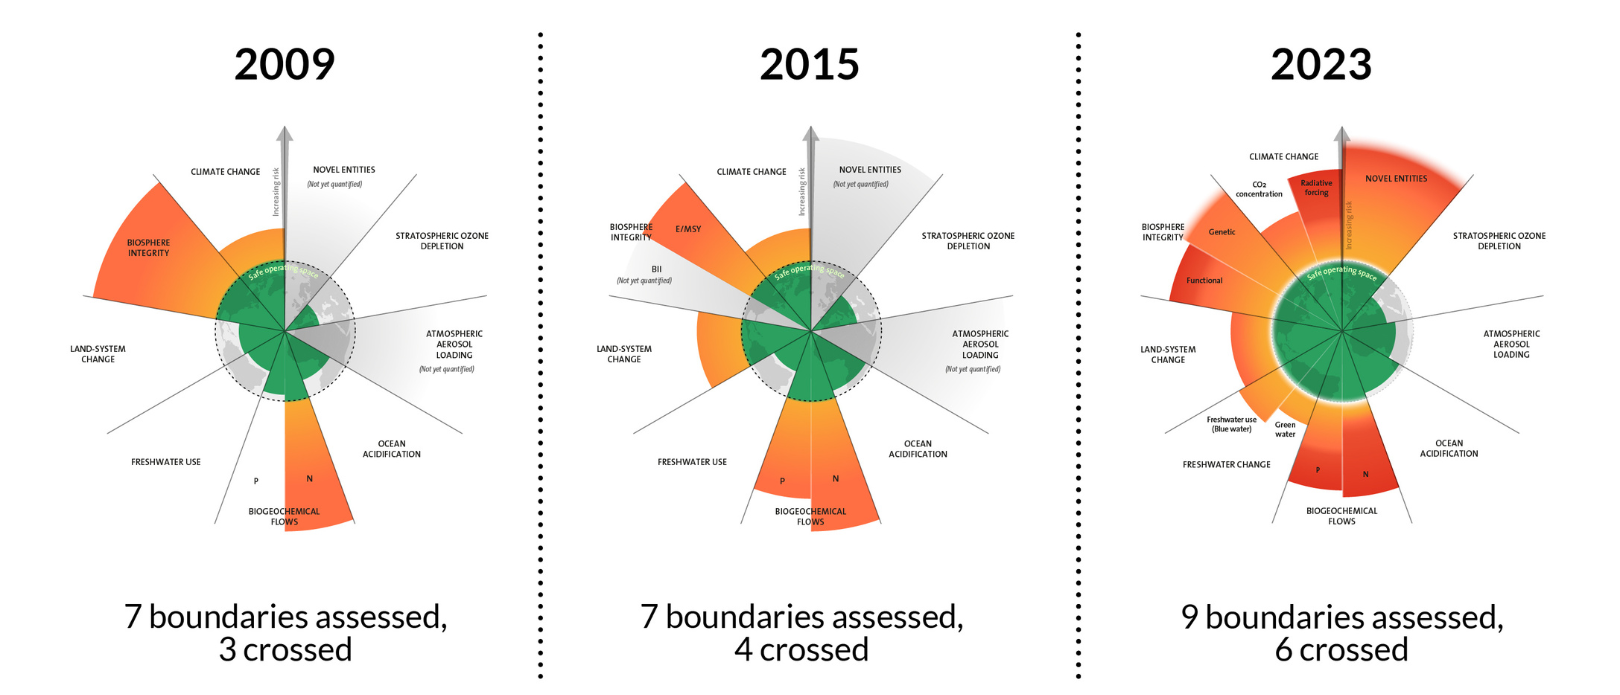
\includegraphics[keepaspectratio]{2_approaches/images/Fig2_1__planetaryboundaries.png}}

}

\caption{\label{fig-development-planetary-boundaries}Entwicklung der
Kontrollvariablen für alle neun planetaren Grenzen. Quelle: Azote für
Stockholm Resilience Centre, Stockholms Universität. Basierend auf
{Rockström, Steffen, Noone, Persson, F. S. I. Chapin, u.~a.} (2009),
{Steffen u.~a.} (2015), Richardson u.~a. (2023). Lizenziert unter CC
BY-NC-ND 3.0.}

\end{figure}%

\subsection{Kipppunkte des Klimasystems der
Erde}\label{kipppunkte-des-klimasystems-der-erde}

\begin{figure}[H]

\centering{

\pandocbounded{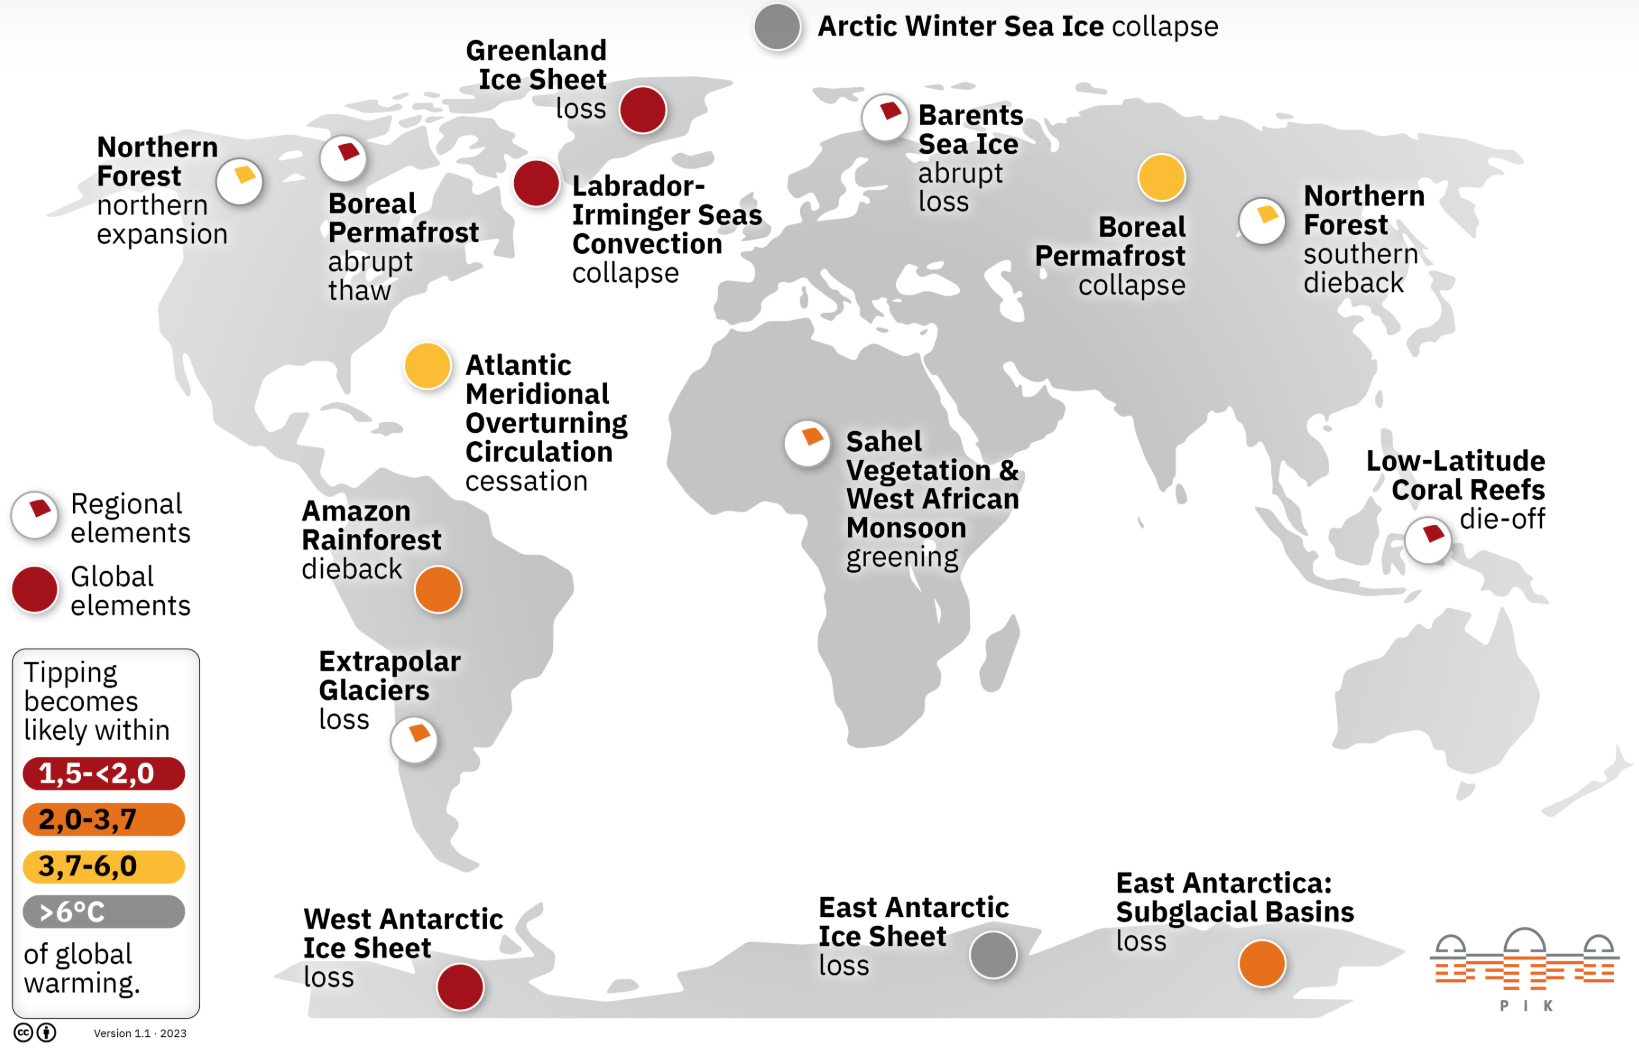
\includegraphics[keepaspectratio]{2_approaches/images/Tippingpoints.png}}

}

\caption{\label{fig-tippingspoints}Räumliche Verteilung globaler und
regionaler Kipppunkte. Die Farben zeigen den Temperaturbereich an, in
dem ein Kippen wahrscheinlich ist. Quelle: Erstellt am PIK, basierend
auf Armstrong McKay u.~a. (2022), erweitert um Wechselwirkungen
basierend auf Lenton u.~a. (2019). Lizenziert unter CC-BY.}

\end{figure}%

Kipppunkte im Klimasystem der Erde sind kritische Schwellen, deren
Überschreitung abrupte und oft irreversible Veränderungen im Klimasystem
auslösen kann. Diese Kipppunkte können das Klima destabilisieren und zu
einem beschleunigten Klimawandel führen. Beispiele für Kipppunkte sind
das Schmelzen des grönländischen Eisschildes, der Kollaps des
Amazonas-Regenwaldes, das Auftauen von Permafrostböden und Veränderungen
im Golfstrom. Wenn diese Kipppunkte erreicht oder überschritten werden,
können sie selbstverstärkende Rückkopplungseffekte auslösen, die zu
weiterer Erwärmung und einer Intensivierung des Klimawandels führen.

Das Konzept der Kipppunkte unterstreicht die Dringlichkeit, die globale
Erwärmung zu begrenzen und die Treibhausgasemissionen zu reduzieren.
Wenn wir die Kipppunkte überschreiten, wird es zunehmend schwieriger,
den Klimawandel zu kontrollieren und seine Auswirkungen zu minimieren.

\subsection{Quantifizierung planetarer
Grenzen}\label{quantifizierung-planetarer-grenzen}

Eine neuere Entwicklung innerhalb des Rahmenwerks der planetaren Grenzen
ist das Konzept der „sicheren und gerechten Erdsystemgrenzen (ESBs)''
für folgende Bereiche: Klima, Biosphäre, Wasser- und Nährstoffkreisläufe
sowie Aerosole auf globaler und subglobaler Ebene (Rockström u.~a.
2023). Die ESBs basieren auf Modellierungen und Literaturauswertungen
und berücksichtigen Unsicherheiten durch unterschiedliche
Wahrscheinlichkeitsniveaus. Die Einhaltung der ESBs schützt Stabilität
und Chancengleichheit zwischen Arten und zukünftigen Generationen,
obwohl gegenwärtige Generationen, insbesondere vulnerable Gruppen,
dennoch Schäden erleiden könnten. Die Autor*innen schlagen daher in
einigen Fällen strengere Grenzen und die Ergänzung durch lokale
Standards zum Schutz der heutigen Generationen und Ökosysteme vor. Sie
identifizieren beispielsweise sichere ESBs für die Erwärmung (Rockström
u.~a. 2023, Fig. 1 and Table 1). Diese basieren auf der Verringerung der
Wahrscheinlichkeit, Klimakipppunkte auszulösen, der Aufrechterhaltung
der Biosphären- und Kryosphärenfunktionen sowie der Berücksichtigung der
Klimavariabilität des Holozäns (\textless0,5--1,0 °C) und früherer
Interglaziale (\textless1,5--2 °C).

Zu den Funktionen der Kryosphäre gehören die Erhaltung des Permafrosts
in den nördlichen Hochbreiten, die Erhaltung der Polareis\-schilde und
Gebirgsgletscher sowie die Minimierung des Meereisverlusts. Die
Autor*innen kommen zu dem Schluss, dass eine globale Erwärmung von mehr
als 1,0 °C über vorindustriellem Niveau, die bereits überschritten wurde
(IPCC 2021), Kippeffekte wie den Kollaps des grönländischen Eisschildes
oder ein lokalisiertes abruptes Auftauen des borealen Permafrosts mit
mässiger Wahrscheinlichkeit auslösen könnte (Armstrong McKay u.~a.
2022). Eine Erwärmung von einem Grad Celsius entspricht der 1990
vorgeschlagenen sicheren Grenze und der planetaren Grenze von 350 ppm
CO\textsubscript{2} ({Steffen u.~a.} 2015). Bei einer Erwärmung von mehr
als 1,5 °C oder 2,0 °C steigt die Wahrscheinlichkeit, Kipppunkte
auszulösen, auf hoch bzw. sehr hoch.

\subsection{Klimaresilienz}\label{klimaresilienz}

Resilienz beschreibt die Fähigkeit eines Systems, Störungen
standzuhalten, sich zu „erholen'' oder aus Widrigkeiten heraus wieder
aufzurichten. Ursprünglich in der Psychologie verwendet, bezeichnet
Resilienz die psychologische Robustheit, die eine Person im Umgang mit
Herausforderungen oder Belastungen, insbesondere in der Kindheit, aktiv
erworben hat. Im Kontext von Ökosystemen bezeichnet Resilienz die
Fähigkeit, Störungen aufzufangen, ohne dass es zu einem dauerhaften
Systemkollaps kommt, d.~h. einem Kollaps, der zu einem anderen, durch
neue Prozesse regulierten System führen würde (Folke u.~a. 2010). In
jüngerer Zeit wurde das Konzept der Resilienz auf soziale Systeme
ausgeweitet (vgl. Abschnitt zur Doughnut-Ökonomie). Studien
konzentrieren sich darauf, welche spezifischen Merkmale einer Region
gestärkt werden müssen, um sie besser auf künftige Krisen und
Katastrophen im Zusammenhang mit Klimawandel, Terrorismus,
Ressourcenknappheit oder Finanzkrisen vorzubereiten. Die Klimakrise
beispielsweise erfordert sowohl Anpassungs- als auch
Minderungsmassnahmen. Resilienzansätze bieten einen Weg, diese beiden
Konzepte miteinander zu verbinden, anstatt sie gegeneinander
auszuspielen.

\textbf{Klimaschutz\-massnahmen} zielen darauf ab,
Treibhausgasemissionen zu reduzieren und den Klimawandel einzudämmen.
Solche Massnahmen umfassen die Förderung erneuerbarer Energien, die
Verbesserung der Energieeffizienz und den Ausbau des öffentlichen
Nahverkehrs. Resilienzansätze betonen die Bedeutung des Klimaschutzes,
da die Begrenzung des Temperaturanstiegs dazu beiträgt, die Intensität
und Häufigkeit von Extremwetterereignissen zu reduzieren.

\textbf{Klimaanpassungsmassnahmen} zielen darauf ab, Gesellschaften und
Ökosysteme widerstandsfähiger gegenüber den aktuellen und erwarteten
Auswirkungen des Klimawandels zu machen. Anpassungsmassnahmen umfassen
die Entwicklung von Frühwarnsystemen für Extremwetterereignisse, den
Küstenschutz vor steigendem Meeresspiegel, die Reduzierung von
Hitzestress (z. B. durch mehr urbane Grünflächen), Rückhaltungs- oder
Versickerungsflächen zur Verringerung der Schadensauswirkungen von
Starkregenereignissen oder die Anpassung landwirtschaftlicher Praktiken
an veränderte Klimabedingungen. Resilienzansätze betonen die
Notwendigkeit der Klimaanpassung, um Gemeinschaften und Ökosysteme vor
den negativen Auswirkungen des Klimawandels zu schützen.

\subsection{Fazit}\label{fazit}

Das Konzept der planetaren Grenzen versucht, komplexe ökologische
Zusammenhänge auf eine kleine Anzahl quantifizierbarer Grenzen zu
reduzieren. Diese spezifischen Grenzen und Indikatoren für planetare
Grenzen basieren auf wissenschaftlichen Erkenntnissen, die nicht immer
eindeutig oder konsistent sind. Die Grenzen werden daher von einigen
Wissenschaftler*innen in Frage gestellt, die die Genauigkeit und
Zuverlässigkeit der verwendeten Daten und Modelle anzweifeln. Trotz
dieser Kritik leistet das Rahmenwerk der planetaren Grenzen einen
wertvollen Beitrag zur Debatte über Nachhaltige Entwicklung und schärft
das Bewusstsein für die begrenzten Ressourcen und die Resilienz unseres
Planeten. Zusammenfassend lässt sich sagen:

\begin{itemize}
\item
  Das Rahmenwerk der planetaren Grenzen fokussiert auf die
  ökologischen/biophysikalischen Grenzen der Resilienz der Erde und
  damit auf die Umweltdimension der Nachhaltigen Entwicklung.
\item
  Diese Resilienzgrenzen -- die planetaren Grenzen -- konzentrieren sich
  auf Umweltfaktoren, die als grundlegend für das menschliche Überleben
  gelten.
\item
  Normativ gesehen zielt das Konzept darauf ab, den stabilen
  Erdsystemzustand („Gleichgewichtszustand'') des Holozäns
  aufrechtzuerhalten und damit Bedrohungen für das menschliche Überleben
  zu mindern.
\item
  Das Rahmenwerk der planetaren Grenzen kann genutzt werden, um konkrete
  Ziele in der Umweltdimension festzulegen (z. B. auf globaler oder
  nationaler Ebene).
\end{itemize}

\begin{tcolorbox}[enhanced jigsaw, arc=.35mm, bottomrule=.15mm, bottomtitle=1mm, breakable, colback=white, colbacktitle=quarto-callout-caution-color!10!white, colframe=quarto-callout-caution-color-frame, coltitle=black, left=2mm, leftrule=.75mm, opacityback=0, opacitybacktitle=0.6, rightrule=.15mm, title={Weiterführende Literatur}, titlerule=0mm, toprule=.15mm, toptitle=1mm]

\begin{itemize}
\item
  Folke, Carl, Stephen R. Carpenter, Brian Walker, Marten Scheffer,
  Terry Chapin, and Johan Rockström. 2010. `Resilience Thinking:
  Integrating Resilience, Adaptability and Transformability'.
  \emph{Ecology and Society} 15 (4).
  \url{https://www.jstor.org/stable/26268226}.
\item
  Lenton, Timothy M., Johan Rockström, Owen Gaffney, et al.~2019.
  `Climate Tipping Points --- Too Risky to Bet Against'. \emph{Nature}
  575 (7784): 7784. \url{https://doi.org/10.1038/d41586-019-03595-0}.
\item
  Rockström, Johan, Joyeeta Gupta, Dahe Qin, et al.~2023. `Safe and Just
  Earth System Boundaries'. \emph{Nature} 619 (7968): 102--11.
  \url{https://doi.org/10.1038/s41586-023-06083-8}.
\end{itemize}

\end{tcolorbox}

\section{Von den planetaren Grenzen zum
Doughnut-Modell}\label{von-den-planetaren-grenzen-zum-doughnut-modell}

Das Doughnut-Modell der Ökonomin Kate Raworth ist ein innovativer Ansatz
zur Nachhaltigen Entwicklung, der soziale und ökologische Grenzen
anerkennt. Dies erfordert, einen Grossteil dessen abzulehnen, was die
Wirtschaft des 20. Jahrhunderts geprägt hat, wie Raworth in ihrem 2017
erschienenen Buch \emph{Doughnut Economics: Seven Ways to Think Like a
21st Century Economist} darlegt. Raworth stellt die ideale Wirtschaft
der Zukunft in einem einfachen Bild dar: einem ringförmigen Doughnut.
Der äussere Ring symbolisiert eine ökologische Decke, die nicht
überschritten werden sollte, da dies der Umwelt irreversiblen Schaden
zufügen würde. Der innere Ring repräsentiert ein soziales Fundament, das
die Grundbedürfnisse der Menschen abdeckt, wie Nahrung, Wohnung und
Einkommen. Die Herausforderung besteht darin, sicherzustellen, dass
wirtschaftliche Aktivitäten innerhalb dieses Rings -- des Doughnuts --
stattfinden, um das Wohlbefinden sowohl der Menschheit als auch der
Umwelt zu gewährleisten („sicherer und gerechter Raum für die
Menschheit'').

\begin{figure}[H]

\centering{

\pandocbounded{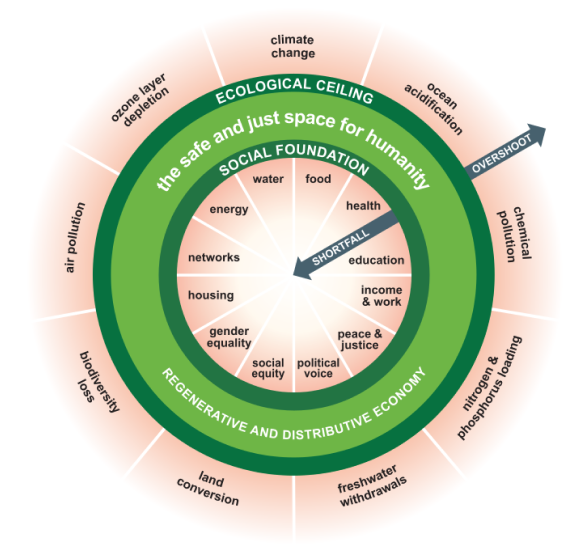
\includegraphics[keepaspectratio]{2_approaches/images/Fig2_3__doughnut.png}}

}

\caption{\label{fig-doughnut}Der Doughnut der sozialen und planetaren
Grenzen. Quelle: \url{https://doughnuteconomics.org}.}

\end{figure}%

Die Philosophie des Doughnut-Ansatzes basiert auf drei Grundprinzipien:
gerechte Verteilung des Wohlstands, Regeneration der von der Wirtschaft
genutzten Ressourcen und Schaffung von Wohlstand für alle Menschen.
Keines dieser Prinzipien sollte von Wirtschaftswachstum abhängig sein,
so Raworth (2017b). Mit anderen Worten: Wir müssen kein unbegrenztes
Wachstum anstreben, damit die Wirtschaft floriert -- stattdessen sollten
wir eine Entwicklung anstreben, die nachhaltig, ausgewogen und gerecht
ist. Der Übergang zum Doughnut-Modell erfordert einen grundlegenden
Wandel in unserer Denk- und Handlungsweise. Es geht darum, vom
Wachstumsparadigma hin zu einer Nachhaltigen Entwicklung zu wechseln,
einer Entwicklung, die soziale Gerechtigkeit und ökologische
Nachhaltigkeit gleichermassen berücksichtigt.

\subsection{Fazit}\label{fazit-1}

Trotz der Fokussierung des Doughnut-Modells auf die Wirtschaft bemängeln
Kritiker*innen, dass es die zugrundeliegenden Rahmenbedingungen (d.~h.
die Strukturen, Regeln und die institutionelle Organisation der
Wirtschaft) oder die Frage, wie Geld geschaffen und verwaltet wird
(d.~h. den Finanzsektor), nicht thematisiert. Das Doughnut-Modell
konzentriert sich darauf, welche Art wirtschaftlicher Aktivität
wünschenswert ist (d.~h. innerhalb des Doughnuts zu bleiben), erklärt
aber nicht, wie man dorthin gelangt. Diese Kritikpunkte werden vom
Doughnut Economics Action Lab (DEAL, o.~J.) aufgegriffen, das Werkzeuge
und Strategien bereitstellt, um das Doughnut-Modell in der Praxis
umzusetzen.

\begin{itemize}
\item
  Das Doughnut-Modell baut auf dem Konzept der planetaren Grenzen auf
  und ergänzt es um eine soziale Dimension sowie um Ziele und Grade der
  Zielerreichung.
\item
  Normativ schreibt das Modell vor, dass

  \begin{itemize}
  \item
    soziale Ziele erreicht werden sollten, ohne die planetaren Grenzen
    zu überschreiten. Die planetaren Grenzen bilden den
    biophysikalischen Rahmen, innerhalb dessen die sozialen Ziele
    erreicht werden sollten.
  \item
    bei der Festlegung konkreter Ziele, Massnahmen usw. auf subglobaler
    Ebene auch die globalen sozialen Ziele berücksichtigt werden müssen.
  \end{itemize}
\end{itemize}

\section{Die Debatte über die Grosse
Transformation}\label{die-debatte-uxfcber-die-grosse-transformation}

Konzepte der „Grossen Transformation'' beziehen sich auf grundlegende
Veränderungen in sozialen, wirtschaftlichen, politischen und
ökologischen Systemen, die notwendig sind, um eine nachhaltige und
gerechte Gesellschaft zu schaffen.

„Grosse Transformation'' war ein Begriff, den Karl Polanyi in seiner
Analyse von 1944 verwendete, wonach der Übergang zu einem freien Markt
im 19. Jahrhundert tiefgreifende soziale, wirtschaftliche und politische
Veränderungen mit sich brachte, die das Leben der Menschen und ihre
Beziehung zur Natur grundlegend veränderten. Polanyi argumentierte, dass
ungezügelte Marktdynamiken soziale und ökologische Probleme verursachten
und dass die Gesellschaft Mechanismen entwickeln müsse, um diese
Probleme zu regulieren und auszugleichen. Ähnlich betonen heutige
Konzepte der Grossen Transformation die Bedeutung von Regulierung,
Umverteilung und der Entwicklung alternativer Wirtschaftsmodelle zur
Schaffung einer nachhaltigen und gerechten Gesellschaft. Während Polanyi
die Notwendigkeit sozialer Schutzmassnahmen und die Bedeutung der
Integration von Märkten in gesellschaftliche Strukturen betonte, zielen
aktuelle Konzepte der Grossen Transformation zusätzlich darauf ab,
Produktions- und Konsummuster grundlegend zu verändern, um die
Umweltbelastung zu reduzieren.

\subsection{\texorpdfstring{WBGU-Hauptgutachten: \emph{Welt im
Wandel}}{WBGU-Hauptgutachten: Welt im Wandel}}\label{wbgu-hauptgutachten-welt-im-wandel}

Das Hauptgutachten des Wissenschaftlichen Beirats der Bundesregierung
Globale Umweltveränderungen (WBGU 2011), \emph{Welt im Wandel}, ist eine
wichtige Publikation, die sich mit den Herausforderungen und Chancen
einer nachhaltigen Transformation der Gesellschaft befasst. Es wurde
erstmals 1994 veröffentlicht und seitdem mehrfach aktualisiert. Das
Gutachten analysiert globale Umweltveränderungen, darunter Klimawandel,
Biodiversitätsverlust und Ressourcenverbrauch, und schlägt konkrete
Politiken und gesellschaftliche Veränderungen zur Förderung einer
Nachhaltigen Entwicklung vor.

\emph{Welt im Wandel} ist für die Debatten über die Grosse
Transformation bedeutsam, da es für eine weitreichende Transformation
von Wirtschaft, Politik und Gesellschaft plädiert. Diese Vision geht
über blosse Anpassung hinaus und fordert grundlegende Veränderungen in
den Strukturen und Mustern wirtschaftlicher Aktivität und des
Alltagslebens. Das Gutachten unterstreicht die Dringlichkeit, den
Übergang zu einer klimafreundlichen und umweltverträglichen Wirtschaft
und Lebensweise voranzutreiben. Es betont die entscheidende Rolle einer
umfassenden Nachhaltigkeitspolitik. Schliesslich identifiziert es
Innovation, Technologie, Bildung, institutionelle Reformen und
internationale Zusammenarbeit als zentrale Hebel zur Erreichung
Nachhaltiger Entwicklung.

\begin{figure}[H]

\centering{

\pandocbounded{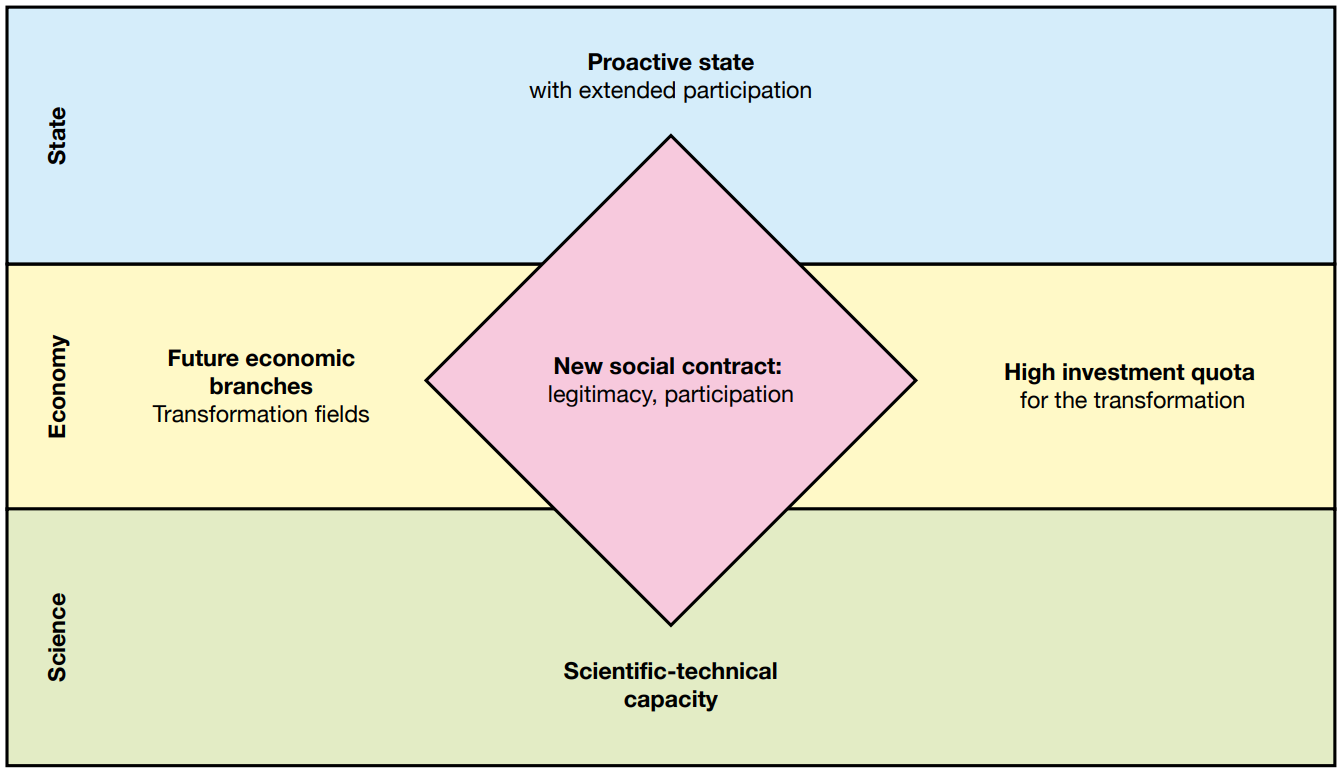
\includegraphics[keepaspectratio]{2_approaches/images/WBGU-social-contract.png}}

}

\caption{\label{fig-new-social-contract}Neuer Gesellschaftsvertrag.
Quelle: WBGU (2011, pp.~275).}

\end{figure}%

In Kapitel 8 unterscheidet \emph{Welt im Wandel} zwischen zwei
Konzepten: „Transformationsforschung und -bildung'' sowie
„transformative Forschung und Bildung''. Diese Konzepte sind
entscheidend für die Förderung eines grundlegenden Wandels hin zur
Nachhaltigkeit.

\emph{Transformationsforschung} analysiert Veränderungsprozesse,
insbesondere im Kontext Nachhaltiger Entwicklung. Sie versucht, die
Dynamik und Komplexität von Transformationen zu verstehen und mögliche
Handlungspfade für eine nachhaltige Zukunft zu identifizieren.
Transformationsforschung bietet eine inter- und transdisziplinäre
Perspektive und bindet verschiedene Akteur*innen und Interessengruppen
in den Forschungsprozess ein.

\emph{Transformationsbildung} ist eine Bildung, die darauf abzielt, das
Wissen, die Fähigkeiten und die Werte zu vermitteln, die für eine
nachhaltige Transformation der Gesellschaft erforderlich sind. Sie
umfasst formale und informelle Bildungsmassnahmen, die es Menschen
ermöglichen, aktiv an Transformationsprozessen teilzuhaben und
nachhaltiges Denken und Handeln zu fördern.

\emph{Transformative Forschung} generiert nicht nur Wissen, sondern geht
einen Schritt weiter und strebt aktiv einen Wandel hin zur
Nachhaltigkeit an. Sie zielt damit darauf ab, die gesellschaftliche
Praxis zu beeinflussen und Lösungen und Innovationen für eine
Nachhaltige Entwicklung zu entwickeln. Transformative Forschung arbeitet
eng mit Partner*innen aus der Praxis zusammen und bemüht sich darum,
Wissen in Handeln zu übersetzen.

\emph{Transformative Bildung} fördert eine Verschiebung von Denkweisen,
Werten und Verhaltensweisen hin zur Nachhaltigkeit. Sie geht über die
blosse Wissensvermittlung hinaus, indem sie auch kritisches Bewusstsein,
Empathie und Handeln für nachhaltige Veränderungen in der Gesellschaft
fördert.

Der WBGU ist der Ansicht, dass der Staat Aufgaben übernehmen sollte, die
von Einzelpersonen oder dem Privatsektor nicht ausreichend erfüllt
werden. Er erkennt an, dass der Staat eine entscheidende Rolle bei der
Schaffung von Rahmenbedingungen und der Gestaltung politischer
Massnahmen zur Förderung Nachhaltiger Entwicklung spielt. Der Staat kann
innovative Lösungen vorantreiben, Investitionen lenken, Regelungen
etablieren und Politiken umsetzen, die eine nachhaltige Transformation
ermöglichen.

\begin{quote}
„Das Wichtige für die Regierung ist nicht, Dinge zu tun, die
Einzelpersonen bereits tun, und diese ein bisschen besser oder ein
bisschen schlechter zu tun; \textbf{sondern die Dinge zu tun, die
derzeit überhaupt nicht getan werden}.'' John M. Keynes, The End of
Laissez-Faire, 1926
\end{quote}

Der WBGU betont jedoch auch, dass ein wirksames staatliches Handeln in
Zusammenarbeit mit anderen Akteur*innen und Interessengruppen erfolgen
sollte, darunter Zivilgesellschaft, Privatwirtschaft und Wissenschaft.
Die gemeinsame Gestaltung einer nachhaltigen Zukunft bedeutet,
Partnerschaften zu schaffen und unterschiedliche Expertise
einzubeziehen.

\subsection{Schneidewinds „Kunst der
Zukunft''}\label{schneidewinds-kunst-der-zukunft}

Der deutsche Ökonom und Politiker Uwe Schneidewind erörtert das Konzept
der Grossen Transformation in seinem 2018 erschienenen Buch \emph{Die
grosse Transformation: Eine Einführung in die Kunst des
gesellschaftlichen Wandels}. Schneidewind (2018) stellt fest, dass eine
Grosse Transformation nicht durch unaufhaltsame Entwicklungsdynamiken
moderner Gesellschaften oder durch einen technokratischen Entwurf für
eine ökologisch gerechte Gesellschaft vorgegeben ist. Stattdessen sieht
er sie als einen Prozess, der von vielen Akteur*innen aktiv gestaltet
werden sollte. Deshalb ist es wichtig, einen klar definierten normativen
Kompass zu haben und die Fähigkeit zu entwickeln, komplexe soziale,
kulturelle, wirtschaftliche und technologische Prozesse zu navigieren.
Er beschreibt diese Fähigkeit als die „Kunst der Zukunft'' -- die
Fertigkeit, wünschenswerte Zukünfte möglich zu machen -- und schlägt
damit eine Brücke zu Harald Welzers FUTURZWEI. Welzer, ein Psychologe
und Soziologe, betont die Bedeutung von Vorstellungskraft, Kreativität
und Engagement bei der Herbeiführung transformativer Veränderungen und
der Entwicklung alternativer Zukunftsvisionen.

\begin{figure}[H]

\centering{

\pandocbounded{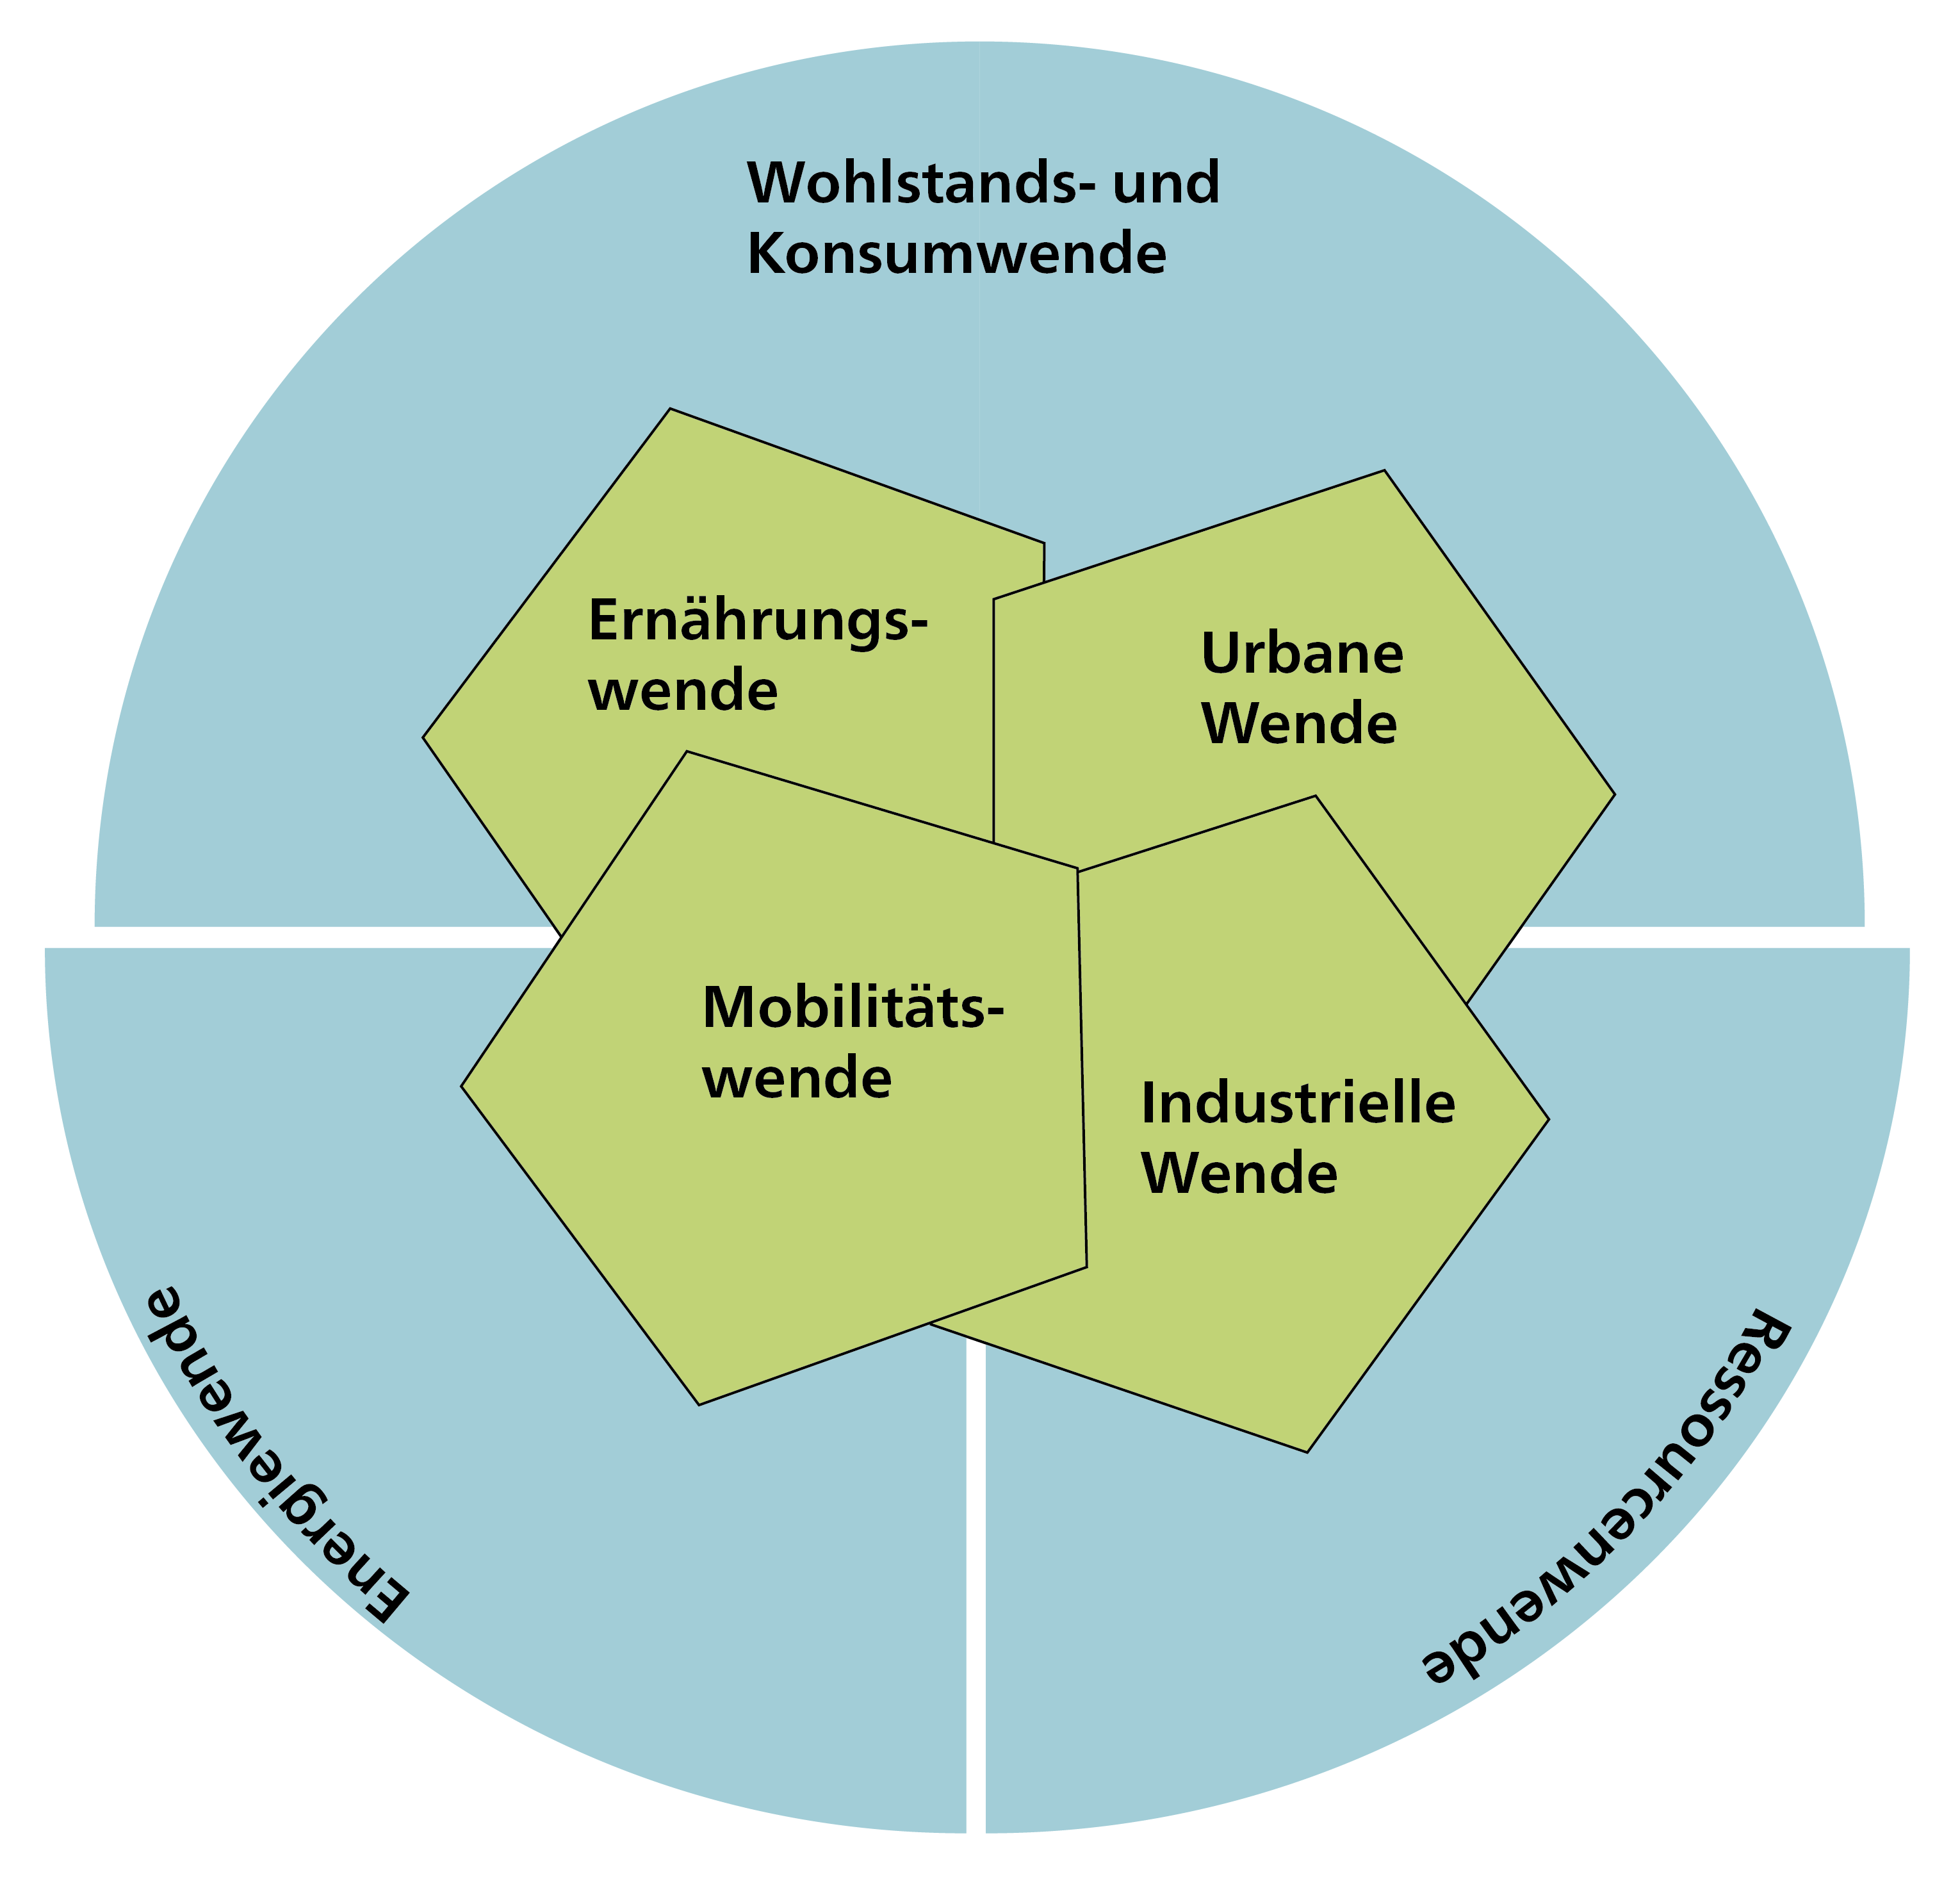
\includegraphics[keepaspectratio]{2_approaches/images/Fig2_5_Schneidewind_turningpoints.png}}

}

\caption{\label{fig-turningpoints}Verständnis des Zusammenspiels der
sieben Wendepunkte der Grossen Transformation. Quelle: Eigene
Darstellung basierend auf Schneidewind (2018).}

\end{figure}%

Für Schneidewind (2018) hat die Grosse Transformation sieben
transformative Wendepunkte. Die vier Dimensionen der „Kunst der
Zukunft'' (technologisch, wirtschaftlich, kulturell, institutionell)
finden sich in allen sieben Wendepunkten wieder. Ressourcen- und
Energietransformationen sind grundlegend. Gemäss dem Konzept der
„doppelten Entkopplung'' sind sie jedoch ohne eine umfassende
Transformation der Vorstellungen von Wohlstand und Konsum nicht denkbar.
Die gewünschte Transformation ist in spezifischeren Sektoren leichter
vorstellbar, wie Mobilität, Ernährung, Städte und wichtige energie- und
ressourcenintensive Industrien.

\begin{figure}[H]

\centering{

\pandocbounded{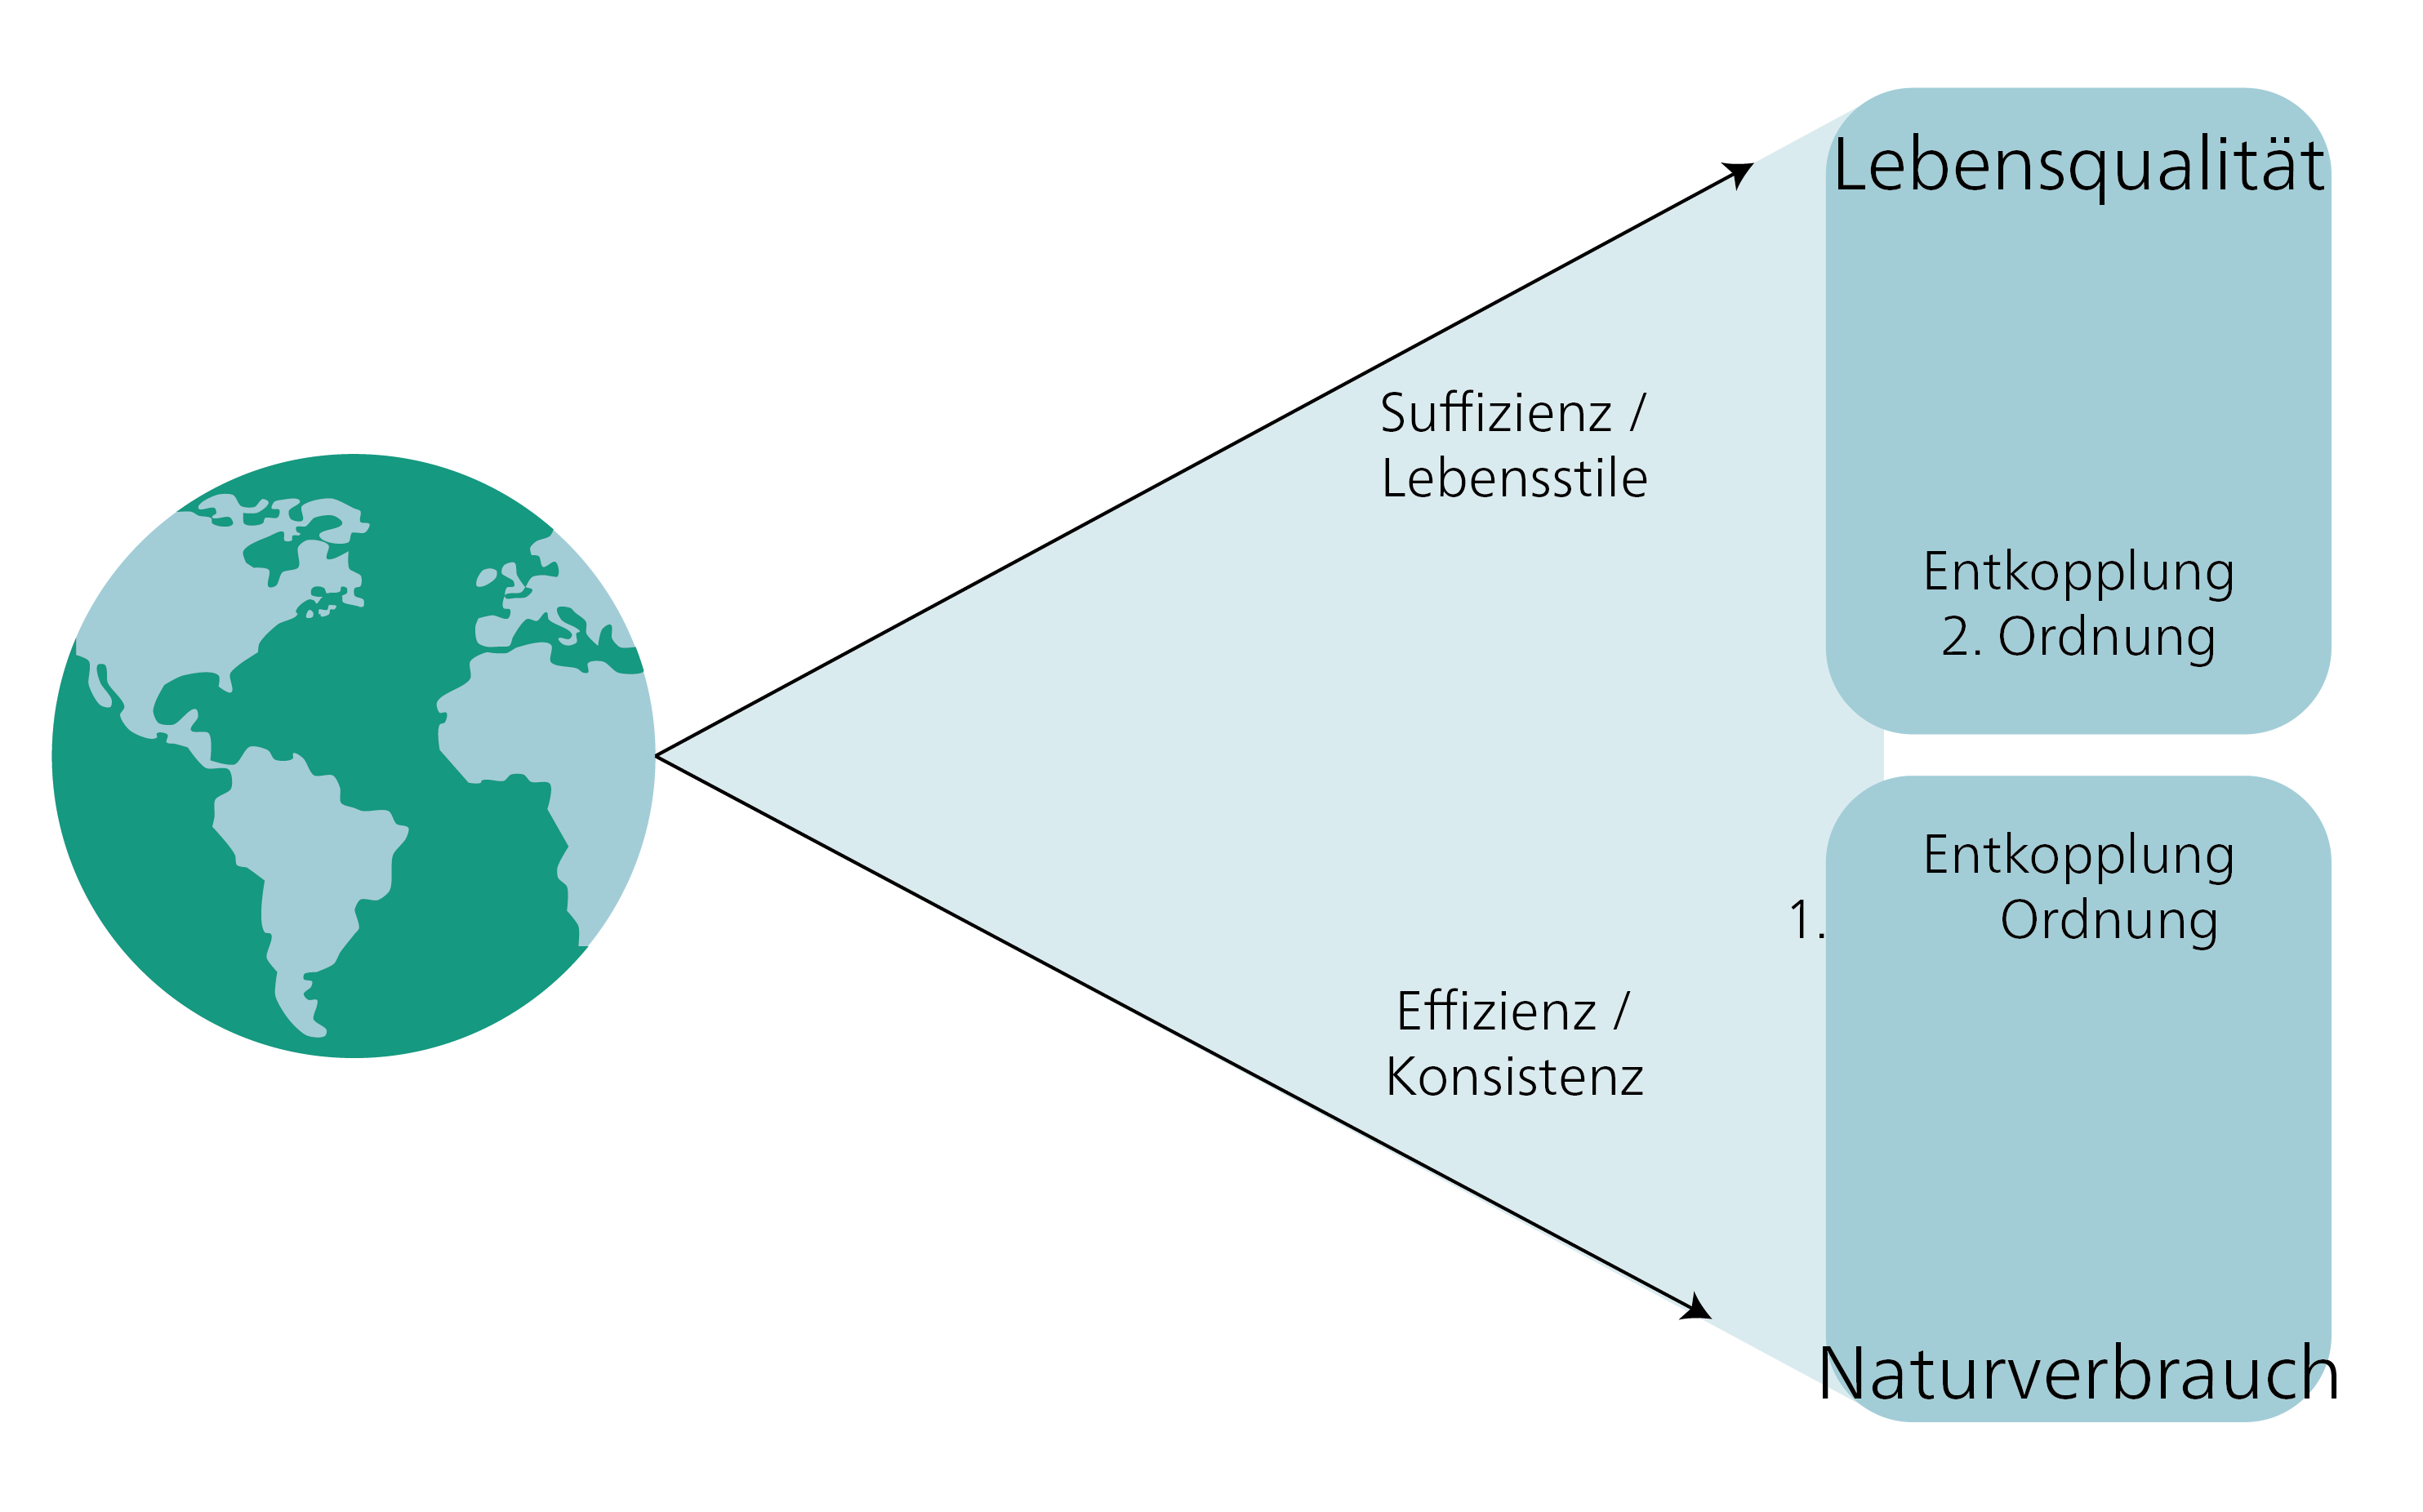
\includegraphics[keepaspectratio]{2_approaches/images/Fig2_6__double_decoupling.png}}

}

\caption{\label{fig-double-decoupling}Doppelte Entkopplung. Verknüpfung
von Technologie und Wohlstandsmodellen. Quelle: Eigene Darstellung
basierend auf Schneidewind (2018).}

\end{figure}%

„Entkopplung'' bezeichnet die Trennung wirtschaftlicher Aktivität von
Umweltauswirkungen. Als zentrales Konzept in der Nachhaltigkeitsdebatte
besagt die \textbf{doppelte Entkopplung}, dass Nachhaltige Entwicklung
nur durch Steigerungen der technologischen Effizienz in Kombination mit
neuen Wohlstands- und Konsummodellen erreicht werden kann. Sie zielt
darauf ab, ein umfassenderes und systemisches Verständnis von Innovation
zu fördern, das sowohl technologische als auch soziale Innovationen
einschliesst.

Die doppelte Entkopplung bezieht sich auf die folgenden zwei Arten der
Entkopplung:

\begin{itemize}
\item
  Entkopplung erster Ordnung: Diese konzentriert sich auf die Steigerung
  der Ressourceneffizienz und -konsistenz innerhalb des traditionellen
  Wirtschaftswachstumsmodells, hauptsächlich durch technologische
  Fortschritte, und
\item
  Entkopplung zweiter Ordnung: Diese konzentriert sich auf „Suffizienz''
  und entkoppelt die Lebensqualität und ein „gutes Leben'' vom
  traditionellen, am BIP gemessenen Wirtschaftswachstumsmodell.
\end{itemize}

\subsection{Global Sustainable Development
Report}\label{global-sustainable-development-report}

Im September 2019 wurde der erste Global Sustainable Development Report
(GSDR) von einer Gruppe von 15 unabhängigen Wissenschaftler*innen
veröffentlicht, die vom UNO-Generalsekretär ernannt wurden. Der GSDR,
der alle vier Jahre erscheinen soll, hat zum Ziel, bestehendes Wissen zu
synthetisieren und Wege zur Erreichung der Ziele für Nachhaltige
Entwicklung (SDGs) aufzuzeigen. Der jüngste Bericht (2023) hebt die
erhebliche Lücke zwischen dem aktuellen Fortschritt und der Erreichung
der SDGs hervor. Aufbauend auf dem Bericht von 2019 führt er den
Kapazitätsaufbau als neuen Hebel zur Beschleunigung des Fortschritts
ein.

\begin{figure}[H]

\centering{

\pandocbounded{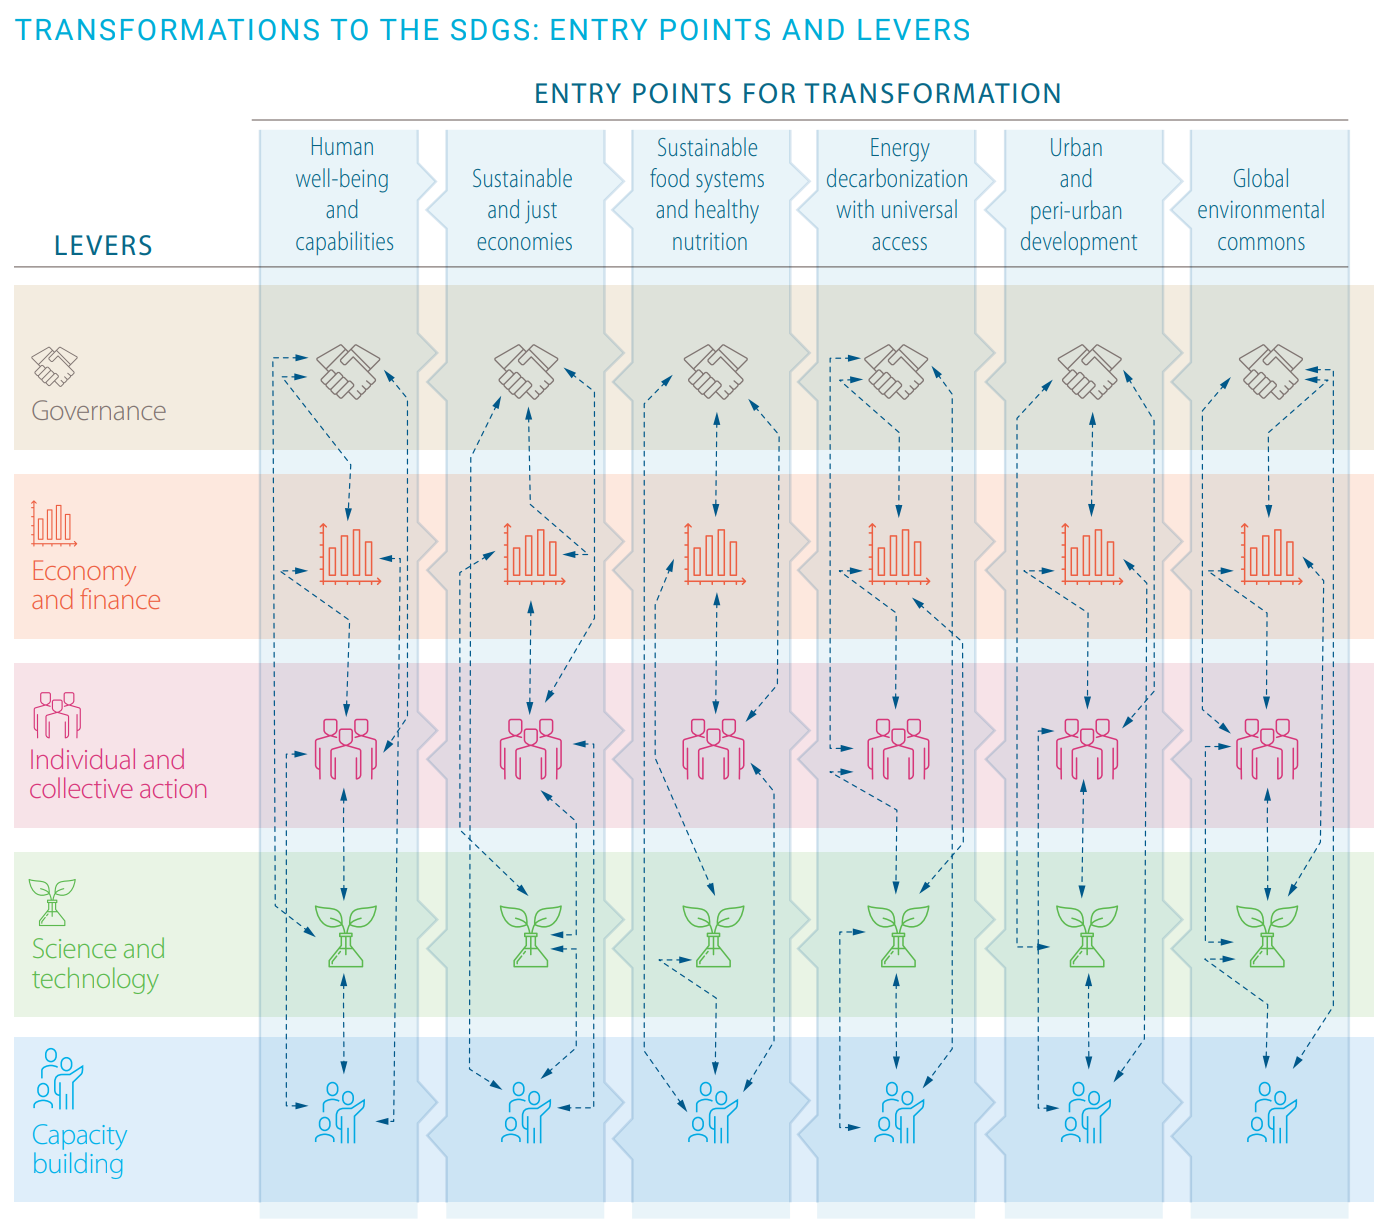
\includegraphics[keepaspectratio]{2_approaches/images/Fig2_7__GSDR.png}}

}

\caption{\label{fig-GSDR}Hebel und Einstiegspunkte zur Erreichung der
SDGs. Quelle: Independent Group of Scientists appointed by the
Secretary-General (2023).}

\end{figure}%

Der GSDR schlägt sechs Schlüsselbereiche oder „Einstiegspunkte'' mit dem
grössten Potenzial vor, die notwendigen umfangreichen und raschen
Transformationen voranzutreiben. Um diese Transformationen einzuleiten,
ist eine aktive und vielseitige Zusammenarbeit zwischen Akteur*innen aus
verschiedenen Bereichen entscheidend: Governance, Wirtschaft und
Finanzen, individuelles und kollektives Handeln sowie Wissenschaft und
Technologie.

\subsection{Fazit}\label{fazit-2}

Konzepte der „Grossen Transformation''

\begin{itemize}
\item
  halten es für notwendig und möglich, die gesellschaftliche Entwicklung
  in Richtung Nachhaltigkeit zu steuern.
\item
  sind ganzheitliche Konzepte zur Steuerung der gesellschaftlichen
  Entwicklung. Sie schlagen Einstiegspunkte in verschiedenen Bereichen
  der Gesellschaft und auf mehreren Handlungsebenen vor.
\item
  schlagen Schlüsselbereiche mit grosser Hebelwirkung vor (z. B. schlägt
  der WBGU eine Energietransformation, eine Stadttransformation, eine
  Landnutzungstransformation und transformative Bildung und Forschung
  vor).
\end{itemize}

\begin{tcolorbox}[enhanced jigsaw, arc=.35mm, bottomrule=.15mm, bottomtitle=1mm, breakable, colback=white, colbacktitle=quarto-callout-caution-color!10!white, colframe=quarto-callout-caution-color-frame, coltitle=black, left=2mm, leftrule=.75mm, opacityback=0, opacitybacktitle=0.6, rightrule=.15mm, title={Weiterführende Literatur}, titlerule=0mm, toprule=.15mm, toptitle=1mm]

\begin{itemize}
\tightlist
\item
  Polanyi, Karl. 1944. \emph{The Great Transformation: The Political and
  Economic Origins of Our Time}. Beacon Press.
\end{itemize}

\end{tcolorbox}

\section{Grüne Wirtschaft}\label{gruxfcne-wirtschaft}

In einem wegweisenden Gebrauch des Begriffs „grüne Wirtschaft''
lancierten David Pearce und Edward Barbier 1989 ihre bahnbrechende
\emph{Blueprint for a Green Economy}-Reihe. Die Reihe war die erste, die
wirtschaftliche Rahmenkonzepte und programmatische Ansätze zur
Erreichung der doppelten Ziele wirtschaftlicher Prosperität und
ökologischen Wohlergehens vorstellte (z. B. Pearce u.~a. 1989, 2000;
Barbier und Markandya 2013). Das Kernprinzip der Grünen Wirtschaft
stellt die traditionelle Ansicht in Frage, dass Wirtschaftswachstum und
ökologisches Wohlergehen grundsätzlich unvereinbar sind. Es schlägt
einen Paradigmenwechsel vor, weg von Verboten und Einschränkungen.
Stattdessen plädiert es für wirtschaftliche Anreize und Strategien, die
die ökologische Nachhaltigkeit fördern und gleichzeitig positive Modelle
wirtschaftlicher und technologischer Entwicklung begünstigen, die sowohl
mit ökologischen als auch mit sozialen Zielen vereinbar sind.

Im Vorfeld von Rio+20, der UNO-Konferenz für Nachhaltige Entwicklung
2012, wurde das Konzept der Grünen Wirtschaft schliesslich zu einem
Leitprinzip entwickelt, das die Debatte prägte (UNEP 2011; Bär u.~a.
2011). „Grüne Wirtschaft'' war eines von zwei Kernthemen von Rio+20; das
andere war der „institutionelle Rahmen'' für Nachhaltige Entwicklung.
Dementsprechend wurden 2011 und 2012 zahlreiche Dokumente zur Grünen
Wirtschaft veröffentlicht, und eine wegweisende Definition des Begriffs
wurde vom Organisationsgremium von Rio+20, dem Umweltprogramm der
Vereinten Nationen (UNEP), im Bericht \emph{Towards a Green Economy:
Pathways to Sustainable Development and Poverty Eradication} (UNEP 2011)
veröffentlicht. Auch die OECD leistete mit ihrer Entschliessung zu
„Grünem Wachstum'' (OECD 2009) einen eigenen Beitrag zur Reaktion auf
die Finanzkrise.

\begin{quote}
„Das UNEP definiert eine grüne Wirtschaft als eine solche, die zu
verbessertem menschlichem Wohlbefinden und sozialer Gerechtigkeit führt
und gleichzeitig Umweltrisiken und ökologische Knappheiten erheblich
reduziert. Im einfachsten Sinne kann eine grüne Wirtschaft als eine
solche verstanden werden, die CO\textsubscript{2}-arm,
ressourceneffizient und sozial inklusiv ist. In einer grünen Wirtschaft
sollten Einkommens- und Beschäftigungswachstum durch öffentliche und
private Investitionen angetrieben werden, die Kohlenstoffemissionen und
Umweltverschmutzung reduzieren, die Energie- und Ressourceneffizienz
verbessern und den Verlust von Biodiversität und Ökosystemleistungen
verhindern.'' (UNEP 2011, p.~2)
\end{quote}

Obwohl Rio+20 das Konzept der Grünen Wirtschaft zementierte, war die
Notwendigkeit eines grundlegenden globalen Umdenkens bereits weitgehend
akzeptiert. Es war deutlich geworden, dass Umweltschutzmassnahmen zwar
Geld kosten, aber auch positive wirtschaftliche Auswirkungen haben,
indem sie Arbeitsplätze schaffen (vgl. z. B. UBA 2008) und Innovationen
in technologischen Effizienzfortschritten anspornen (vgl. z. B. {von
Weizsäcker u.~a.} 1995). Das Konzept der Grünen Wirtschaft
systematisiert solche Erkenntnisse und fordert Programme, um die
scheinbaren Widersprüche zwischen Wirtschaft und Ökologie, Wachstum und
Ressourcenschonung sowie Wohlstand und Umweltschutz zu überwinden. Das
Konzept markiert damit einen bedeutenden Paradigmenwechsel. Die
Einhaltung planetarer Grenzen oder ökologischer Leitlinien in einer
Grünen Wirtschaft bedeutet nicht zwangsläufig, auf Wirtschaftswachstum
und technologischen Fortschritt zu verzichten (Rockström, Steffen,
Noone, Persson, F. S. Chapin, u.~a. 2009; SRU 2012). Stattdessen lautet
die Idee, dass wir durch die Harmonisierung dieser scheinbar
widersprüchlichen Ziele sie noch effizienter erreichen können. Der EU
Green Deal exemplifiziert dieses Konzept. Die EU strebt an, bis 2050 der
erste klimaneutrale Kontinent zu werden, mit dem Ziel einer modernen,
ressourceneffizienten und wettbewerbsfähigen Wirtschaft mit netto null
Treibhausgasemissionen. Dieser Plan soll Wachstum vom
Ressourcenverbrauch entkoppeln und gleichzeitig einen gerechten Übergang
gewährleisten, der niemanden zurücklässt.

\subsection{Fazit}\label{fazit-3}

Die Kernthese der Grünen Wirtschaft lautet, dass ökologische und
wirtschaftliche Ziele kein Widerspruch sind. Stattdessen können sie
durch geeignete wirtschaftliche Anreize und Strategien miteinander
vereinbart werden. Die Grüne Wirtschaft zielt darauf ab, sowohl
Wirtschaftswachstum als auch ökologische Nachhaltigkeit durch
öffentliche und private Investitionen in emissionsarme,
ressourceneffiziente und sozial gerechte Wirtschaftssysteme zu fördern.

Kritiker*innen haben jedoch Bedenken hinsichtlich der Wirksamkeit von
Massnahmen der Grünen Wirtschaft geäussert. Sie argumentieren, dass die
vorgeschlagenen Technologien und Anreize nicht ausreichen, um die
notwendigen weitreichenden systemischen Veränderungen herbeizuführen.
Eine übermässige Betonung von Wirtschaftswachstum und technologischen
Lösungen könnte wesentliche strukturelle und verhaltensbezogene
Veränderungen vernachlässigen. Und sie warnen, dass der globale Übergang
zu einer Grünen Wirtschaft benachteiligte Gemeinschaften und
Entwicklungsländer zurücklassen könnte, wenn deren spezifische
Bedürfnisse nicht berücksichtigt werden.

\section{Postwachstumsgesellschaften}\label{postwachstumsgesellschaften}

Die Postwachstumsdebatte entstand aus Bedenken, die in den 1970er Jahren
nach der Veröffentlichung des einflussreichen Meadows-Berichts \emph{The
Limits to Growth} (1972) aufkamen. Wie bereits erwähnt, wies dieser
Bericht auf die begrenzte Kapazität der Erde hin, die Menschheit
angesichts eines ungezügelten Wirtschaftswachstums zu tragen.

Die Postwachstumsdebatte befürwortet qualitatives Wachstum oder sogar
Nullwachstum und kritisiert die Auswirkungen der „modernen'' Wirtschaft
und Lebensweise (z. B. Daly 1999). Sie argumentiert, dass der Zwang zu
ständigem Wachstum dazu führt, dass wir ökologische Grenzen
überschreiten, was zu negativen sozialen und ökologischen Konsequenzen
führt. „Ökologische Ökonomie'' ist in diesem Zusammenhang ein wichtiges
Konzept, da sie alternative Modelle und Ansätze zur Bewertung des
Wirtschaftswachstums zu entwickeln versucht.

Das Dilemma in dieser Debatte besteht darin, dass die meisten Ansätze
für eine nachhaltige Wirtschaft davon ausgehen, dass eine
wachstumsunabhängige Wirtschaft nicht profitorientiert sein sollte.
Kapitalistische Wirtschaften sind jedoch existenziell auf Wachstum
angewiesen Oberholzer (2021). Dieses Dilemma ist der Kern der Frage, wie
ein erfolgreicher Übergang vom aktuellen nicht nachhaltigen System zu
einem nachhaltigen Wirtschafts- und Gesellschaftssystem organisiert
werden kann. Ein Hauptansatz besteht darin, Wachstumsabhängigkeiten zu
reduzieren und alternative Modelle zu fördern, die auf Suffizienz
ausgerichtet sind, ohne dabei Strategien zu vernachlässigen, die sich
auf Effizienz und Konsistenz konzentrieren. Dies erfordert Veränderungen
in Produktions- und Konsummustern, in sozialen Normen und im politischen
Rahmen. Die Postwachstumsdebatte betont die Notwendigkeit einer
umfassenden Transformation, die ökologische, soziale und wirtschaftliche
Dimensionen umfasst -- und darauf abzielt, ein Gleichgewicht zwischen
menschlichen Bedürfnissen und planetaren Grenzen zu erreichen.

Das Konzept der „Suffizienz'' ist ein integraler Bestandteil der
Postwachstumsdebatte (Schneidewind und Zahrnt 2013). Suffizienz zielt
darauf ab, Überkonsum zu reduzieren und alternative Lebensstile,
Konsumgewohnheiten und Produktionsmuster zu fördern. Um eine
weitverbreitete Akzeptanz von Suffizienz zu fördern, ist ein rechtlicher
und institutioneller Rahmen erforderlich, der suffizienzorientierte
Praktiken anreizt und erleichtert.

\begin{figure}[H]

\centering{

\pandocbounded{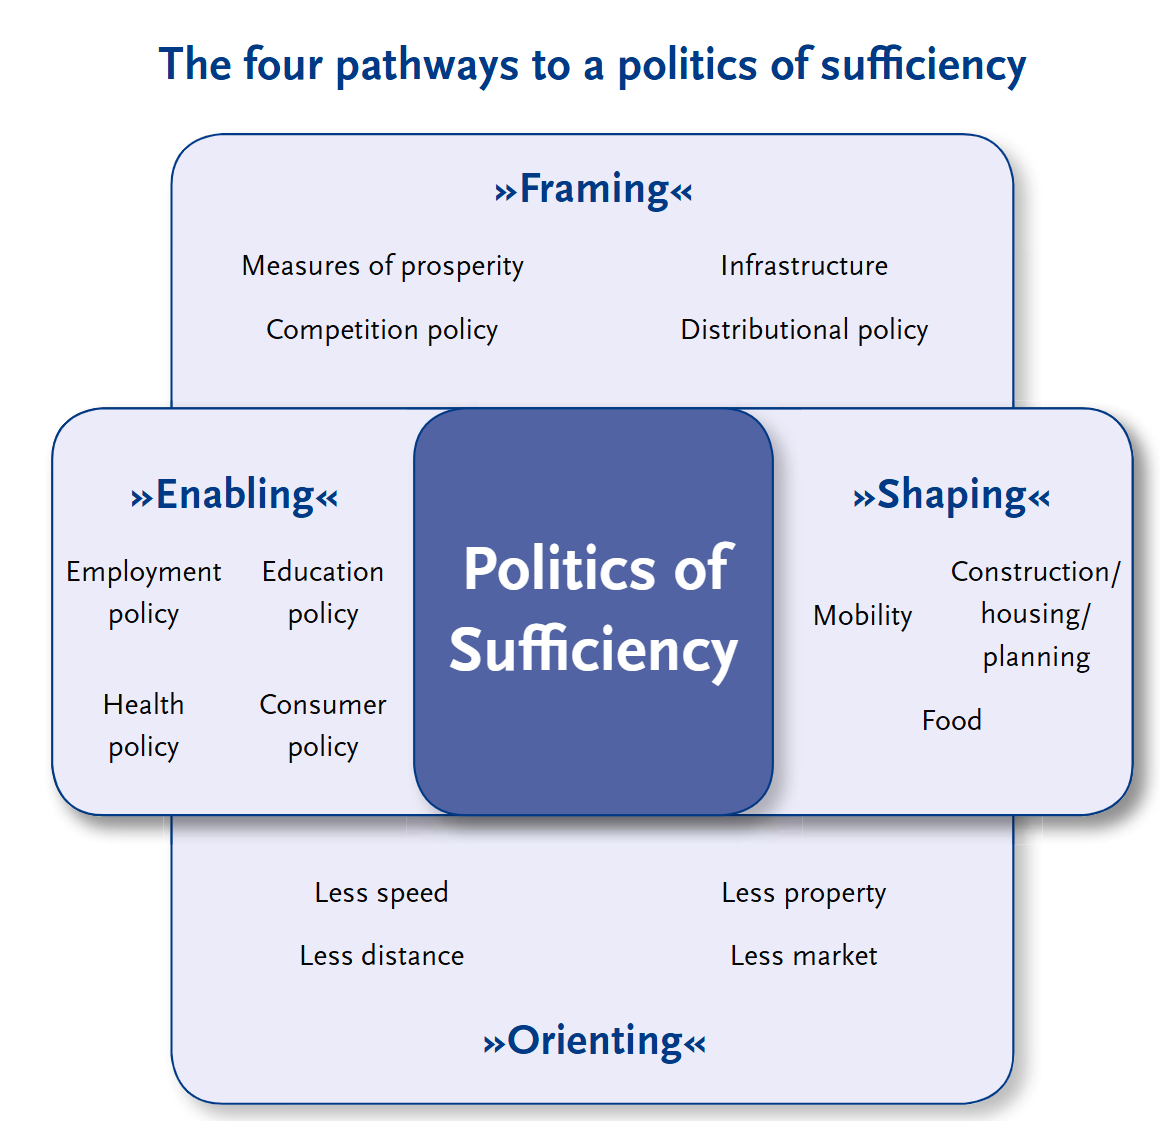
\includegraphics[keepaspectratio]{2_approaches/images/Fig2_8__PoliticsSufficiency.png}}

}

\caption{\label{fig-development-planetary-boundaries}Die vier Bereiche
einer Suffizienzpolitik. Quelle: Schneidewind und Zahrnt (2014)}

\end{figure}%

Eine Politik zur Förderung von Suffizienz kann unsere Entscheidungen
aktiv gestalten, durch attraktive suffizienzorientierte Angebote und
Dienstleistungen. Sie kann auch das Bewusstsein schärfen und
Orientierung für die Übernahme suffizienzorientierter Lebensstile und
Praktiken bieten. Dieser umfassende Ansatz zielt darauf ab, den Konsum
auf das Notwendige und Sinnvolle zu lenken und so den übermässigen
Ressourcenverbrauch zu reduzieren.

\subsection{Fazit}\label{fazit-4}

Postwachstumsdebatten analysieren und kritisieren die Abhängigkeit der
modernen Gesellschaft vom Wirtschaftswachstum sowie die negativen
ökologischen und sozialen Auswirkungen dieses Wachstums. Anstatt sich
ausschliesslich auf technologischen Fortschritt und Marktkräfte zu
verlassen, streben Theorien der Postwachstumsgesellschaft nach
Veränderungen in Gesellschaft, Strukturen und institutionellen
Rahmenbedingungen. Insgesamt betonen Postwachstumsdebatten die
Notwendigkeit nachhaltiger Ansätze, um eine umfassende Transformation
von Wirtschaft und Gesellschaft zu erreichen. Die Transformation zu
einer Postwachstumsgesellschaft erfordert eine Neuausrichtung von
Werten, Strukturen und institutionellen Rahmenbedingungen. Die
Herausforderung besteht darin, Wege zu finden, den Übergang zu einer
wachstumsunabhängigen Wirtschaft zu gestalten und gleichzeitig soziale
Gerechtigkeit und ökologische Nachhaltigkeit zu gewährleisten.

Kritiker*innen der Postwachstumsdebatten argumentieren, dass eine
Ablehnung des Wirtschaftswachstums negative Auswirkungen auf Wohlstand
und sozialen Fortschritt haben könnte. Sie befürchten, dass eine
wachstumsunabhängige Wirtschaft zu stagnierender Innovation, weniger
Arbeitsplätzen und sinkenden Lebensstandards führen könnte. Und sie
weisen auf die potenziell negativen Auswirkungen einer negativen
Einstellung gegenüber Wirtschaftswachstum hin. Die konstruktive
Auseinandersetzung mit den Herausforderungen des Wachstums und die
Entwicklung gangbarer Alternativen sind wichtige Aspekte, um einen
nachhaltigen und gerechten Wandel zu ermöglichen.

\section{Indikatoren für Nachhaltige Entwicklung: Von Prinzipien zur
Praxis}\label{indikatoren-fuxfcr-nachhaltige-entwicklung-von-prinzipien-zur-praxis}

Ein zentrales Anliegen der Nachhaltigen Entwicklung ist die Fähigkeit,
sowohl Fortschritte als auch Rückschritte systematisch sichtbar zu
machen -- auf globaler, nationaler und lokaler Ebene. Indikatoren
spielen dabei eine entscheidende Rolle: Sie helfen, komplexe
sozial-ökologische Realitäten zu erfassen, ermöglichen Vergleichbarkeit
und unterstützen evidenzbasierte Politikgestaltung. Da Nachhaltigkeit
ein normatives Ziel ist, ist bei der Auswahl, Gestaltung und Nutzung von
Indikatoren besondere Sorgfalt geboten.

Wichtig ist: Indikatoren sind keine rein technischen Messinstrumente.
Sie spiegeln unweigerlich spezifische Werte, Weltbilder und politische
Ziele wider. Ihre Aussagekraft basiert nicht allein auf „objektiven
Daten'', sondern auch auf Entscheidungen darüber, was, wie und zu
welchem Zweck gemessen werden soll. So hat das Bruttoinlandsprodukt
(BIP) lange Zeit als wichtigstes Massstab für wirtschaftlichen Erfolg
dominiert -- obwohl es ökologische Schäden, soziale Ungleichheit,
unbezahlte Sorgearbeit und Ökosystemleistungen ausser Acht lässt.

In der Nachhaltigkeitswissenschaft und der Umweltpolitik hat sich eine
nützliche Unterscheidung zwischen verschiedenen Indikatorentypen
herausgebildet, die jeweils eine spezifische Funktion erfüllen ({de
Vries} 2024):

\begin{itemize}
\item
  \textbf{Zustandsindikatoren} beschreiben den Zustand eines Systems
  oder einer Ressource -- etwa die CO₂-Konzentration in der Atmosphäre,
  den Anteil geschützter Waldfläche oder die durchschnittliche
  Lebenserwartung. Sie werden vor allem zur Überwachung von Trends und
  Systemzuständen verwendet.
\item
  \textbf{Ursachenindikatoren} erfassen zugrundeliegende Treiber oder
  Einflussfaktoren, die zu Veränderungen in einem System führen. Dazu
  gehören beispielsweise der Verbrauch fossiler Brennstoffe oder
  sozioökonomische Treiber wie Urbanisierungsraten oder Konsummuster.
\item
  \textbf{Input- oder Interventionsindikatoren} beziehen sich auf
  institutionelle oder politische Massnahmen, die als Reaktion auf
  Probleme eingeführt werden. Beispiele sind Subventionen für
  erneuerbare Energien, gesetzliche Regelungen oder öffentliche
  Aufklärungskampagnen. Sie verfolgen das Vorhandensein und die Art von
  Interventionen.
\item
  \textbf{Leistungs- oder Outputindikatoren} messen die Ergebnisse oder
  Auswirkungen dieser Interventionen im Verhältnis zu vordefinierten
  Zielen. Dazu können Emissionsreduktionen, der Anteil recycelter
  Materialien oder Fortschritte bei der sozialen Gerechtigkeit gehören.
\end{itemize}

Diese Klassifikation verdeutlicht, dass einzelne Indikatoren isoliert
betrachtet oft wenig aussagekräftig sind. Erst das Zusammenspiel von
Indikatoren -- z. B. innerhalb von Wirkungsmodellen oder kausalen
Rahmenkonzepten -- ermöglicht eine robuste Beurteilung von
Nachhaltigkeitstrends und politischen Reaktionen.

In den vergangenen Jahrzehnten wurde eine breite Palette alternativer
Indikatorensysteme entwickelt, um ein umfassenderes Bild der
gesellschaftlichen Entwicklung jenseits des BIP zu liefern. Diese
Ansätze zielen darauf ab, wirtschaftliche, soziale und ökologische
Dimensionen zu integrieren und dabei Verteilungseffekte und
nicht-marktliche Beiträge sichtbar zu machen.

Ein bedeutender Meilenstein war die Entwicklung des \textbf{Human
Development Index (HDI)} durch das Entwicklungsprogramm der Vereinten
Nationen (UNDP) in den 1990er Jahren. Der HDI kombiniert drei
Dimensionen: Lebenserwartung bei der Geburt (als Proxy für Gesundheit),
durchschnittliche und erwartete Schuljahre (Bildung) sowie
Pro-Kopf-Einkommen, kaufkraftbereinigt (materieller Lebensstandard). Der
HDI sollte den engen monetären Fokus des BIP erweitern, indem er ein
fähigkeitsorientiertes Entwicklungsverständnis als „Erweiterung der
Wahlmöglichkeiten der Menschen'' anbietet (Sen 1999). Bis heute bleibt
er ein Standardreferenzpunkt in der Entwicklungsökonomie (vgl. UNDP
Human Development Reports seit 1990).

Ein weiterführender Ansatz ist der \textbf{Genuine Progress Indicator
(GPI)}, der beim persönlichen Konsum ansetzt (wie das BIP), aber externe
Kosten wie Umweltzerstörung, Ressourcenverbrauch, Kriminalität und
Einkommensungleichheit abzieht, um das Verhältnis von Kosten und Nutzen
des Wirtschaftswachstums offenzulegen. Er berücksichtigt zudem den Wert
unbezahlter Leistungen wie Hausarbeit und ehrenamtliches Engagement.
Erstmals von Daly und Cobb (1989) als Sustainable Economic Welfare
(ISEW) vorgeschlagen, ist der GPI in der ökologischen Ökonomie etabliert
(vgl. Talberth u.~a. 2007). Im Gegensatz zum BIP, das typischerweise im
Laufe der Zeit steigt, stagniert oder sinkt der GPI in vielen
Hocheinkommensländern seit den 1980er Jahren -- was auf eine mögliche
Entkopplung von Wachstum und Wohlbefinden hindeutet.

\begin{figure}[H]

\centering{

\pandocbounded{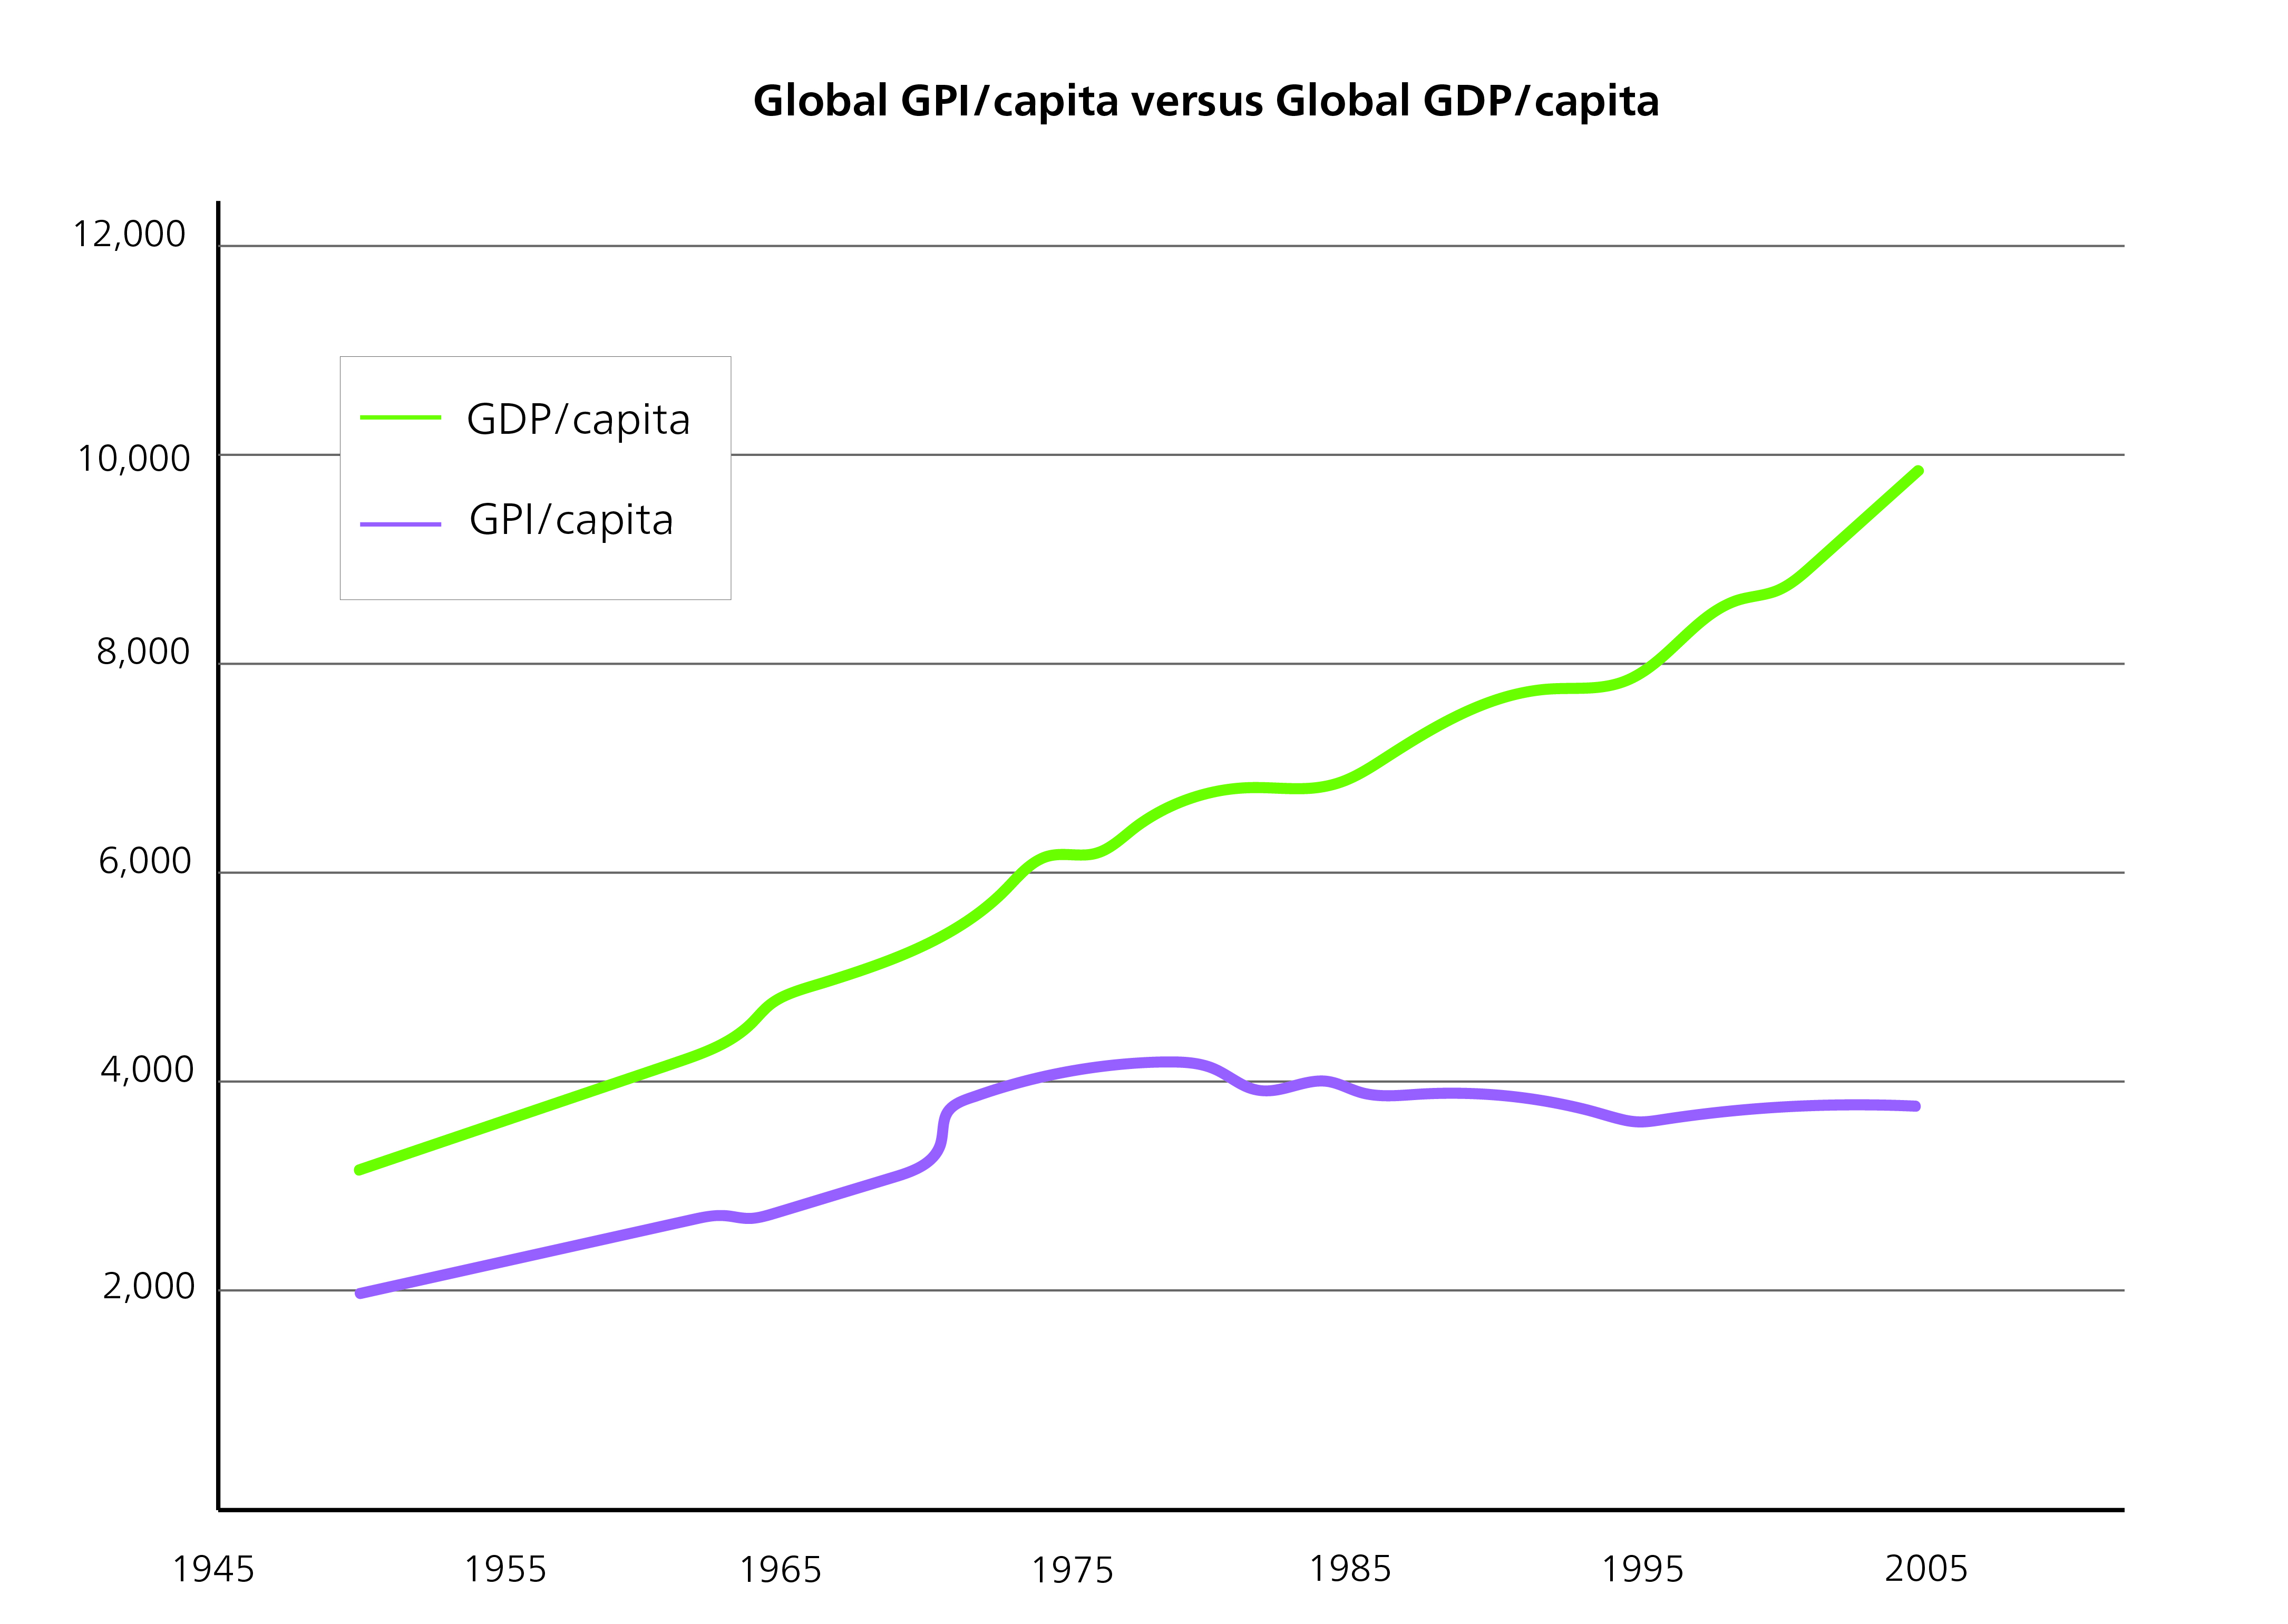
\includegraphics[keepaspectratio]{2_approaches/images/Fig2_9__GDPxGPI.jpg}}

}

\caption{\label{fig-GDPxGPI}Vergleich von globalem Bruttoinlandsprodukt
(BIP) und Genuine Progress Indicator (GPI). Quelle: Eigene Darstellung
basierend auf Kubiszewski u.~a. (2017)}

\end{figure}%

Ein weiteres häufig verwendetes Mass ist der \textbf{Ökologische
Fussabdruck}, der den menschlichen Ressourcenverbrauch in globale Hektar
umrechnet. Er steht für die biologisch produktive Fläche, die benötigt
wird, um den Ressourcenbedarf einer Person, Region oder eines Landes zu
decken -- einschliesslich Fläche für Nahrungsmittelproduktion,
Siedlungen und Kohlenstoffabsorption. Entwickelt von Wackernagel und
Rees (1996) und gefördert durch das Global Footprint Network, ist er
insbesondere in der Umweltbildung weit verbreitet. Der Ökologische
Fussabdruck zeigt auf, ob eine Bevölkerung innerhalb ihrer ökologischen
Verhältnisse lebt -- d.~h. ob sie ihren gerechten Anteil an der globalen
Biokapazität überschreitet.

\begin{figure}[H]

\centering{

\pandocbounded{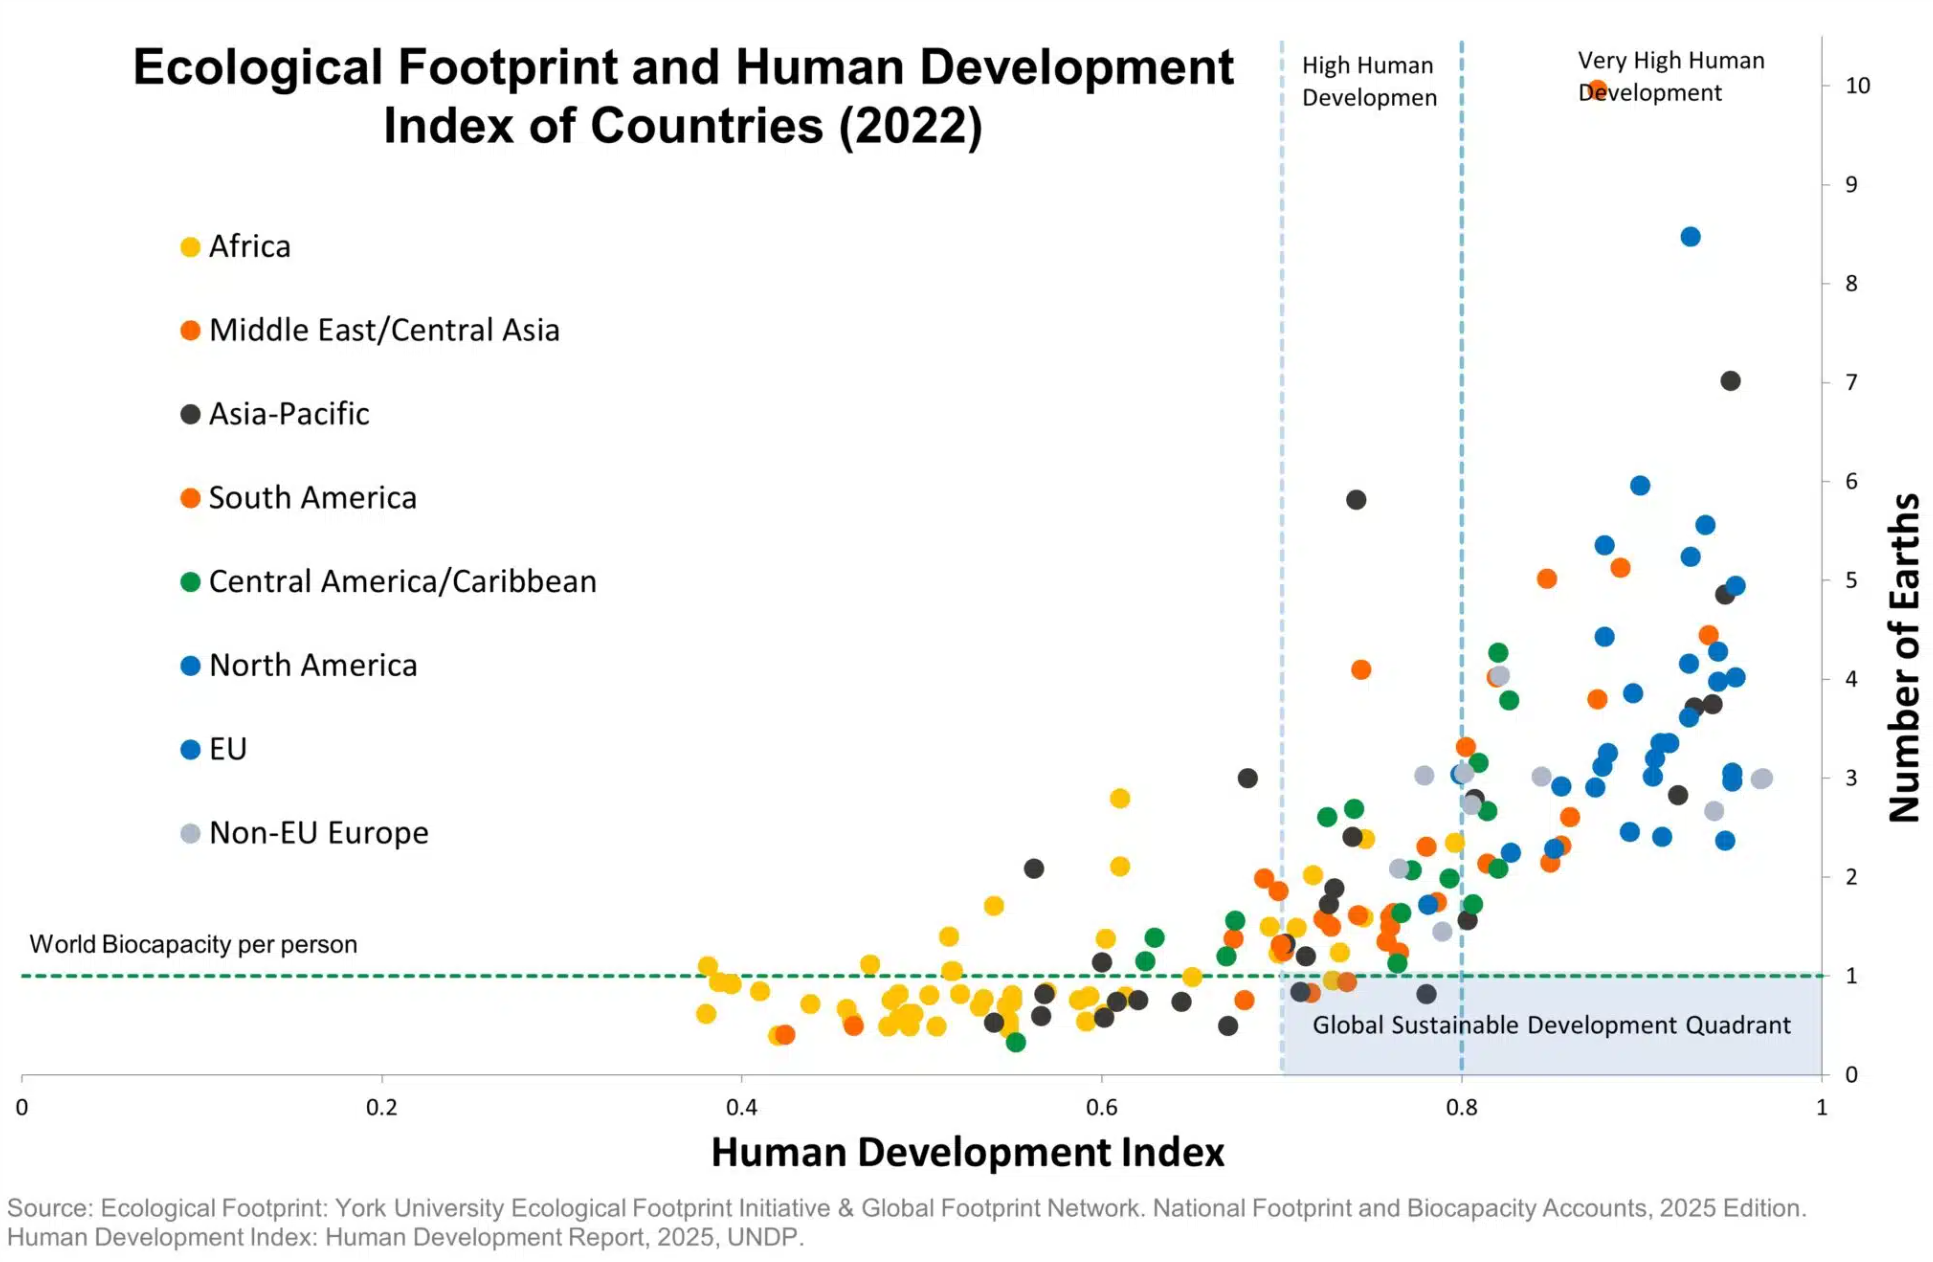
\includegraphics[keepaspectratio]{2_approaches/images/Fig2_10__EcoFootprintHDI.png}}

}

\caption{\label{fig-EcoFootprintHDI}Zusammenhang zwischen Ökologischem
Fussabdruck und Human Development Index (Quelle:
https://www.footprintnetwork.org)}

\end{figure}%

Der \textbf{Happy Planet Index (HPI)} bietet einen subjektiveren Ansatz
und kombiniert Lebenszufriedenheit (auf Umfragebasis), Lebenserwartung
und Ökologischen Fussabdruck, um das „Wohlbefinden pro Einheit
Umweltverbrauch'' zu berechnen. Entwickelt von der New Economics
Foundation zeigt der HPI, dass eine hohe Lebenszufriedenheit nicht
zwangsläufig einen hohen Ressourcenverbrauch erfordert.
Mitteleinkommensländer wie Costa Rica schneiden häufig besser ab als
Industrienationen mit nicht nachhaltigen Konsummustern (NEF 2006).

Im deutschsprachigen Raum wurde der \textbf{Nationale Wohlfahrtsindex
(NWI)} als ein auf nationale Datenverfügbarkeit angepasstes
GPI-Instrument eingeführt. Er umfasst Dimensionen wie
Einkommensverteilung, Umweltbelastung und Gesundheitskosten. Der NWI
wurde ursprünglich vom Institut für ökologische Wirtschaftsforschung
(IÖW) und dem Forschungszentrum für Umweltpolitik (FFU) an der FU Berlin
entwickelt und in mehreren deutschen Bundesländern erprobt (Diefenbacher
und Zieschank 2011).

Ein weiteres besonders relevantes Mass ist der \textbf{Multidimensionale
Armutsindex (MPI)}, der von der Oxford Poverty and Human Development
Initiative (OPHI) in Zusammenarbeit mit dem UNDP entwickelt wurde. Er
erfasst Armut in drei Kerndimensionen: Gesundheit, Bildung und
Lebensstandard. Zu den Indikatoren gehören Kindersterblichkeit,
Schulbesuch, Zugang zu Elektrizität und Wohnbedingungen. Im Gegensatz zu
einkommensbasierten Massstäben bietet der MPI ein differenzierteres
Verständnis von Deprivation über sich überschneidende Dimensionen
hinweg. Bader u.~a. (2017) zeigen den Wert des MPI in einer
Längsschnittstudie zur Armut in der Demokratischen Volksrepublik Laos,
die aufzeigt, wie schnelles Wirtschaftswachstum die Einkommensarmut
verringerte und gleichzeitig Disparitäten in Bildung, Infrastruktur und
Gesundheitsversorgung verschärfte.

\begin{tcolorbox}[enhanced jigsaw, arc=.35mm, bottomrule=.15mm, bottomtitle=1mm, breakable, colback=white, colbacktitle=quarto-callout-tip-color!10!white, colframe=quarto-callout-tip-color-frame, coltitle=black, left=2mm, leftrule=.75mm, opacityback=0, opacitybacktitle=0.6, rightrule=.15mm, title={Der Ökologische Fussabdruck -- Erklärung und Kritik}, titlerule=0mm, toprule=.15mm, toptitle=1mm]

Der \textbf{Ökologische Fussabdruck} misst, wie viel biologisch
produktive Land- und Meeresfläche (in globalen Hektar) benötigt wird, um
den Ressourcenverbrauch einer Person, Bevölkerung oder eines Landes im
Laufe der Zeit aufrechtzuerhalten. Er umfasst die für die
CO₂-Absorption, Nahrungsmittelproduktion, Infrastruktur und andere
menschliche Bedürfnisse benötigte Fläche. Das Konzept wurde in den
1990er Jahren von Mathis Wackernagel und William Rees entwickelt und ist
eines der bekanntesten Instrumente für die Umweltkommunikation geworden.

Der Ökologische Fussabdruck wird häufig in öffentlichen
Aufklärungskampagnen verwendet, insbesondere im Zusammenhang mit dem
jährlich veröffentlichten \emph{Earth Overshoot Day} -- dem symbolischen
Datum, an dem der Ressourcenverbrauch der Menschheit die Fähigkeit der
Erde zur Regeneration dieser Ressourcen im selben Jahr übersteigt.

\textbf{Wesentliche Einschränkungen des Indikators gemäss Global
Footprint Network (2020):}

\begin{itemize}
\item
  Nicht-ökologische Aspekte der Nachhaltigkeit: Ein Fussabdruck, der
  kleiner als die Biosphäre ist, ist eine notwendige
  Mindestvoraussetzung für eine nachhaltige Gesellschaft, aber nicht
  hinreichend. So berücksichtigt der Ökologische Fussabdruck
  beispielsweise kein soziales Wohlbefinden. Darüber hinaus kann auf der
  Ressourcenseite selbst dann, wenn der Ökologische Fussabdruck
  innerhalb der Biokapazität liegt, schlechtes Management zu einer
  Erschöpfung führen. Ein Fussabdruck kleiner als die Biokapazität ist
  lediglich eine notwendige Bedingung, damit Qualitätsverbesserungen
  replizierbar und skalierbar sind.
\item
  Erschöpfung nicht erneuerbarer Ressourcen: Der Fussabdruck verfolgt
  nicht die Menge nicht erneuerbarer Ressourcenvorräte wie Öl, Erdgas,
  Kohle oder Metallvorkommen. Der mit diesen Materialien verbundene
  Fussabdruck basiert auf der genutzten oder durch ihre Gewinnung
  beeinträchtigten Regenerationskapazität und im Fall fossiler
  Brennstoffe auf der für die Assimilation der von ihnen erzeugten
  Abfälle benötigten Fläche.
\item
  Inhärent nicht nachhaltige Aktivitäten: Aktivitäten, die inhärent
  nicht nachhaltig sind, wie die Freisetzung von Schwermetallen,
  radioaktiven Materialien und persistenten synthetischen Verbindungen
  (z. B. Chlordan, polychlorierte Biphenyle (PCBs),
  Fluorchlorkohlenwasserstoffe (FCKW), Polyvinylchlorid (PVC), Dioxine
  usw.), gehen nicht direkt in die Fussabdruckberechnungen ein. Diese
  Aktivitäten müssen unabhängig von ihrer Menge beendet werden (es gibt
  kein Biokapazitätsbudget für ihre Nutzung). Wo diese Substanzen jedoch
  zu einem Verlust an Biokapazität führen, ist ihr Einfluss bei der
  zukünftigen Messung der Biokapazität erkennbar.
\item
  Ökologische Degradation: Der Fussabdruck misst ökologische
  Degradation, wie erhöhte Bodenversalzung durch Bewässerung, die die
  zukünftige Bioproduktivität beeinflussen könnte, nicht direkt. Wenn
  die Degradation jedoch zu einem Rückgang der Bioproduktivität führt,
  wird dieser Verlust bei der zukünftigen Messung der Biokapazität
  erfasst. Darüber hinaus kann „Unternutzung'' in einem Bereich (z. B.
  Wälder) bei alleiniger Betrachtung der Gesamtzahl eine Übernutzung in
  einem anderen Bereich (z. B. Fischerei) verbergen.
\item
  Resilienz von Ökosystemen: Fussabdruckberechnungen geben nicht an, wo
  und auf welche Weise die Kapazität von Ökosystemen anfällig oder
  resilient ist. Der Fussabdruck ist lediglich ein Ergebnismassstab, der
  dokumentiert, wie viel von der Biosphäre im Verhältnis zu ihrer
  Produktivität genutzt wird.
\end{itemize}

Trotz dieser Einschränkungen bleibt der Ökologische Fussabdruck ein
nützlicher Ausgangspunkt für die Einbeziehung eines breiteren Publikums
in Diskussionen über globale ökologische Gerechtigkeit und planetare
Verantwortung -- insbesondere in Bildungs- und Kommunikationskontexten.

\end{tcolorbox}

\section{Zwischen Vereinfachung und Komplexität: Wechselwirkungen
zwischen den
SDGs}\label{zwischen-vereinfachung-und-komplexituxe4t-wechselwirkungen-zwischen-den-sdgs}

Eine zentrale Herausforderung bei der Gestaltung von
Nachhaltigkeitsindikatoren liegt in der Balance zwischen Vereinfachung
und Komplexität. Indikatoren sollen Entscheidungsprozesse unterstützen,
müssen dabei aber ein breites Spektrum an Wechselwirkungen,
Unsicherheiten und kontextuellen Abhängigkeiten berücksichtigen.

Dies zeigt sich besonders deutlich in der Agenda 2030 für Nachhaltige
Entwicklung. Während die Agenda 17 eigenständige Ziele und zahlreiche
Unterziele umfasst, existieren diese Ziele nicht isoliert. Vielmehr sind
sie komplex miteinander verflochten: Fortschritte in einem Bereich
können Fortschritte in einem anderen verstärken, neutralisieren oder
behindern. Daher sind Indikatoren, die diese Beziehungen beleuchten, für
eine kohärente Politikgestaltung unverzichtbar.

Breu u.~a. (2020) stellen eine Methodik vor, die auf dem von Nilsson
u.~a. (2016) entwickelten Interaktionsrahmen basiert und die Beziehungen
zwischen SDGs auf einer Sieben-Punkte-Skala systematisch klassifiziert:
von stark negativ (--3) bis stark positiv (+3). Sie wendeten diesen
Ansatz auf den nationalen Nachhaltigkeitsrahmen der Schweiz an und
zeigten dabei Bereiche auf, in denen politische Massnahmen für ein SDG
andere unterstützen oder mit ihnen in Konflikt geraten können.
Massnahmen zur Armutsreduzierung (SDG 1) könnten beispielsweise mit
Biodiversitätszielen (SDG 15) in Konflikt geraten, wenn sie nicht
ökologisch nachhaltig gestaltet werden.

\section{Grundlagen der Nachhaltigkeit: Das Quiz -- Kapitel
2}\label{grundlagen-der-nachhaltigkeit-das-quiz-kapitel-2}

Welche zwei planetaren Grenzen gelten als „Kerngrenzen''?

\begin{itemize}
\tightlist
\item[$\square$]
  Ozonabbau und Landnutzung
\item[$\square$]
  Ozeanversauerung und Stickstoffkreisläufe
\item[$\square$]
  Süsswasser und Aerosole
\item[$\square$]
  Klimawandel und Integrität der Biosphäre
\end{itemize}

Innerhalb des Rahmenwerks der planetaren Grenzen gelten Klimawandel und
Integrität der Biosphäre als Kerngrenzen, da sie eine grundlegende Rolle
bei der Regulierung des Zustands des Erdsystems spielen und die übrigen
planetaren Grenzen stark beeinflussen.

\begin{itemize}
\tightlist
\item
  False
\item
  False
\item
  False
\item
  True
\end{itemize}

Welche der folgenden gehört NICHT zu den neun planetaren Grenzen, die
von Rockström et al.~identifiziert wurden?

\begin{itemize}
\tightlist
\item[$\square$]
  Globale Finanzstabilität
\item[$\square$]
  Integrität der Biosphäre
\item[$\square$]
  Ozeanversauerung
\item[$\square$]
  Klimawandel
\end{itemize}

Das Rahmenwerk der planetaren Grenzen identifiziert biophysikalische
Erdsystemprozesse, die die Stabilität und Resilienz des Planeten
regulieren. Klimawandel, Ozeanversauerung und die Integrität der
Biosphäre sind Teil dieses Rahmenwerks, während globale Finanzstabilität
keine planetare Grenze ist.

\begin{itemize}
\tightlist
\item
  True
\item
  False
\item
  False
\item
  False
\end{itemize}

Welcher der folgenden Kipppunkte gehört NICHT zum Klimasystem der Erde?

\begin{itemize}
\tightlist
\item[$\square$]
  Kollaps des Golfstroms
\item[$\square$]
  Verschmutzung der Ozeane durch Plastik
\item[$\square$]
  Kollaps des Amazonas-Regenwaldes
\item[$\square$]
  Abschmelzen des grönländischen Eisschilds
\end{itemize}

Kipppunkte im Klimasystem der Erde bezeichnen grossräumige Komponenten
des Klimas, die abrupte und potenziell irreversible Veränderungen
durchlaufen können. Der grönländische Eisschild, der Golfstrom (AMOC)
und der Amazonas-Regenwald gelten allesamt als häufig diskutierte
klimatische Kippelemente, während die Verschmutzung der Ozeane durch
Plastik zwar ein Umweltproblem, aber kein Kipppunkt des Klimasystems
ist.

\begin{itemize}
\tightlist
\item
  False
\item
  True
\item
  False
\item
  False
\end{itemize}

Welcher Begriff bezeichnet die Entkopplung von Wirtschaftswachstum und
Umweltschäden bei gleichzeitiger Wahrung des Wohlstands?

\begin{itemize}
\tightlist
\item[$\square$]
  Doppelte Entkopplung
\item[$\square$]
  Grüne Wirtschaft
\item[$\square$]
  Planetare Grenzen
\item[$\square$]
  Resilienz
\end{itemize}

Das Konzept der Grünen Wirtschaft bezeichnet ein Wirtschaftsmodell, das
Wirtschaftswachstum und menschliches Wohlergehen bei gleichzeitiger
Verringerung von Umweltrisiken und ökologischer Knappheit anstrebt und
damit Wohlstand von Umweltschäden entkoppelt.

\begin{itemize}
\tightlist
\item
  False
\item
  True
\item
  False
\item
  False
\end{itemize}

Wofür steht der innere Ring des Doughnut-Modells?

\begin{itemize}
\tightlist
\item[$\square$]
  Das soziale Fundament
\item[$\square$]
  Die ökologische Decke
\item[$\square$]
  Der sichere und gerechte Raum für die Menschheit
\item[$\square$]
  Die planetaren Grenzen
\end{itemize}

Im Doughnut-Modell repräsentiert der innere Ring das soziale Fundament,
das die minimalen sozialen Standards definiert, die für ein gerechtes
und würdevolles Leben aller Menschen notwendig sind.

\begin{itemize}
\tightlist
\item
  True
\item
  False
\item
  False
\item
  False
\end{itemize}

Welche der folgenden Aussagen beschreiben Postwachstumsansätze? (Mehr
als eine Aussage kann richtig sein.)

\begin{itemize}
\tightlist
\item[$\square$]
  Fokus auf Suffizienz und Wohlbefinden
\item[$\square$]
  Eintreten für strukturellen Wandel
\item[$\square$]
  Kritik an der Wachstumsabhängigkeit
\item[$\square$]
  Betonung des BIP-Wachstums
\end{itemize}

Postwachstumsansätze stellen die Abhängigkeit moderner Gesellschaften
von kontinuierlichem Wirtschaftswachstum kritisch infrage. Sie betonen
Suffizienz, Wohlbefinden und Lebensqualität anstelle von BIP-Wachstum
und fordern strukturelle Veränderungen der wirtschaftlichen und sozialen
Systeme, um nachhaltige und gerechte Zukünfte zu ermöglichen.

\begin{itemize}
\tightlist
\item
  True
\item
  True
\item
  True
\item
  False
\end{itemize}

\part{Handlungsfelder der Nachhaltigkeit: Analyse und Strategien zur
Transformation von (un-)nachhaltigen Systemen}

\chapter{Ökologische
Nachhaltigkeit}\label{uxf6kologische-nachhaltigkeit}

Die Wirtschaft ist nicht nur in die Gesellschaft, sondern auch in die
Natur eingebettet. Menschen sind Lebewesen und daher auf materielle
Ressourcen angewiesen, um ihre Bedürfnisse zu erfüllen. Sie benötigen
ausserdem intakte Ökosysteme und ein für menschliche Besiedlung
geeignetes Klima. Wenn wir von „ökologischer Nachhaltigkeit'' sprechen,
meinen wir im Allgemeinen den Schutz der Vielfalt und Funktionsfähigkeit
natürlicher Ökosysteme und der von ihnen bereitgestellten
Dienstleistungen für künftige Generationen. Dies ist eine
anthropozentrische Definition, da sie sich auf menschliche Aktivitäten
konzentriert und darauf, wie diese die langfristige Nachhaltigkeit der
Natur zum Nutzen des Menschen sicherstellen sollen. Diese Perspektive
spiegelt sich auch in unserem Alltag und unserer dualistischen Trennung
von „Mensch'' und „Umwelt'' wider, eine Trennung, die auf das 19.
Jahrhundert zurückgeht und bis heute anhält. So unterteilen wir die
Wissenschaft beispielsweise in „Naturwissenschaften'' und
„Sozialwissenschaften'', und unsere Analysen konzeptualisieren
Umweltschäden oft als „Externalitäten''. Ein anderes Verständnis von
ökologischer Nachhaltigkeit betont die Bedeutung der Aufrechterhaltung
der Selbstregulierung des Erdklimasystems. Diese Sichtweise hebt die
Wechselwirkungen und Rückkopplungen zwischen verschiedenen Komponenten
des Erdklimasystems hervor.

\section{Die normative Dimension ökologischer
Nachhaltigkeit}\label{die-normative-dimension-uxf6kologischer-nachhaltigkeit}

Obwohl unser Verständnis der Funktionsweise von Ökosystemen auf
gründlich erforschten empirischen Informationen basiert (und damit
„Systemwissen'' darstellt), bleibt ökologische Nachhaltigkeit ein
normatives Konzept. Das bedeutet, dass sie nicht nur auf
wissenschaftlichen Erkenntnissen, sondern auch auf einer ethischen
Beurteilung beruht (Abbildung~\ref{fig-normative-dimension}). Die
verschiedenen Interpretationen ökologischer Nachhaltigkeit bieten
unterschiedliche Antworten auf die Frage, was erhalten werden sollte und
warum. Jeder Ansatz zur ökologischen Nachhaltigkeit drückt daher den
angestrebten Zustand der ökologischen Umwelt aus, sowohl heute als auch
in der Zukunft -- welche Aspekte der Natur von der Gegenwart in die
Zukunft erhalten oder bewahrt werden sollen. Wenn wir beispielsweise
über Ökosystemdienstleistungen sprechen, ist die Absicht oft, Ökosysteme
so zu erhalten, dass sie unser eigenes Wohlergehen weiterhin
unterstützen und aufrechterhalten (in diesem Sinne ist es eine
anthropozentrische Perspektive).

\begin{figure}[H]

\centering{

\pandocbounded{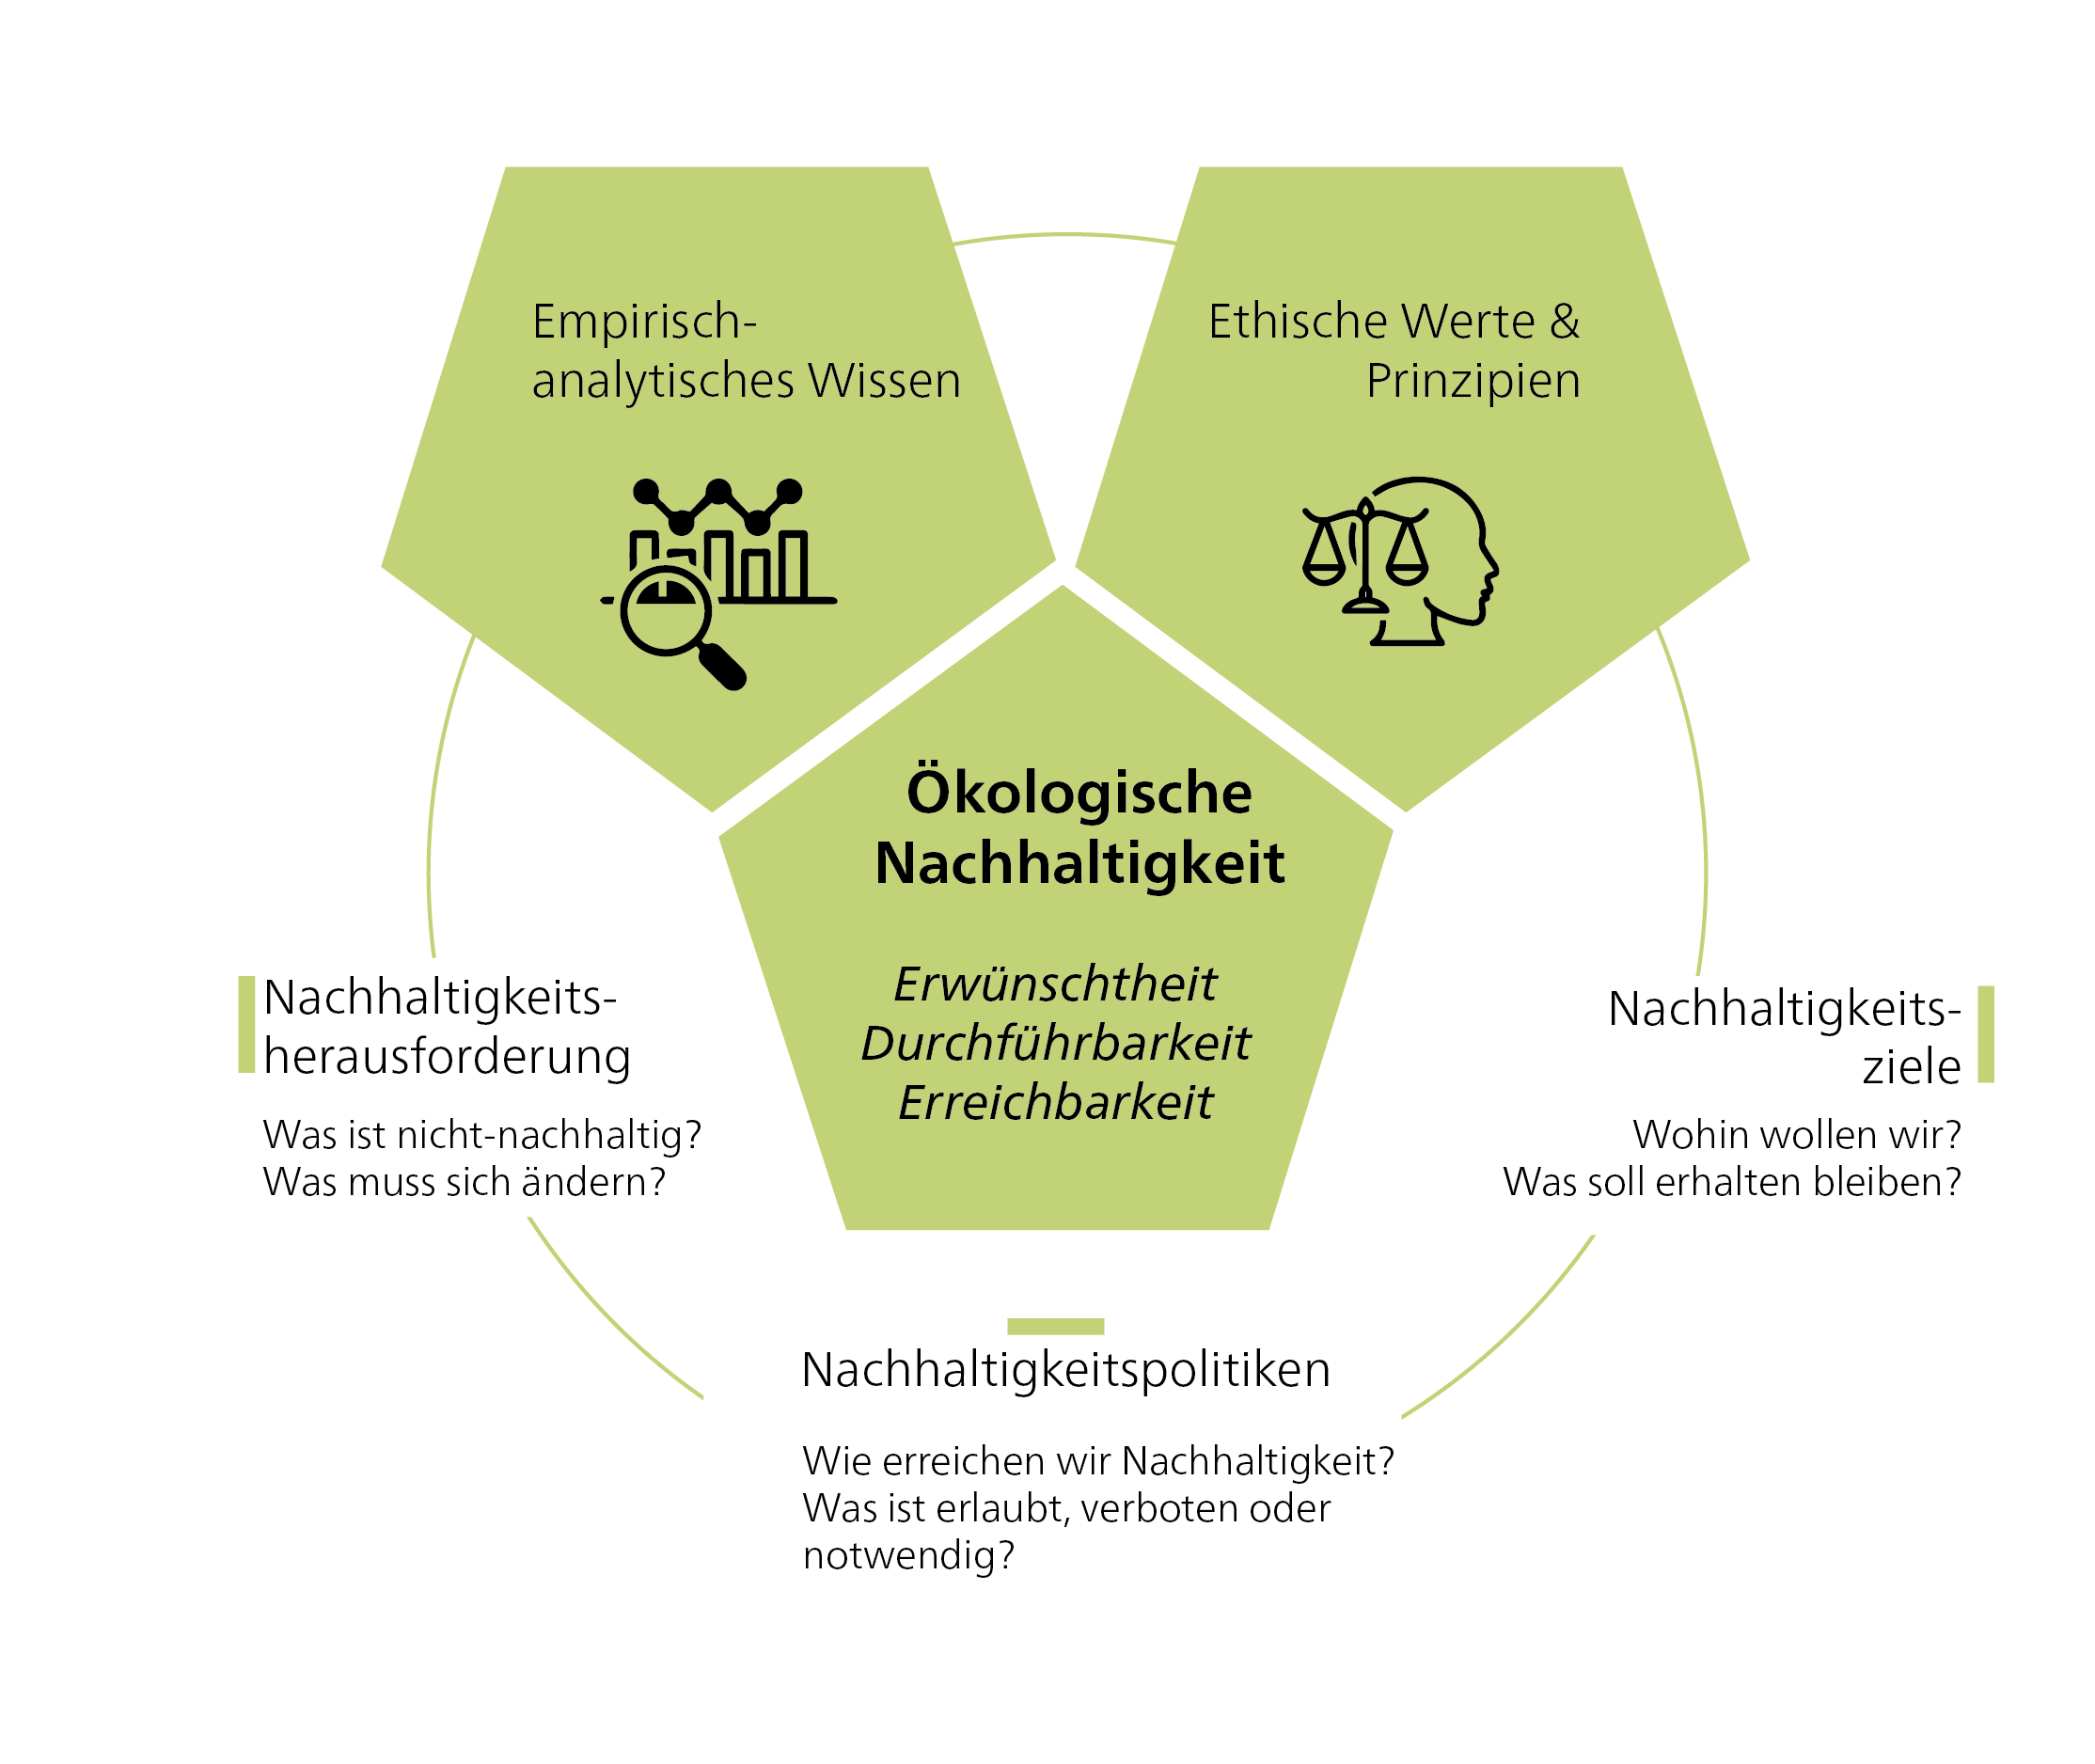
\includegraphics[keepaspectratio]{3_ecological-sustainability/images/Fig3_1__NEecology.png}}

}

\caption{\label{fig-normative-dimension}Die normative Dimension
ökologischer Nachhaltigkeit. Quelle: Eigene Darstellung.}

\end{figure}%

Ethische Urteile und Begründungen prägen, welche ökologischen
Eigenschaften und Funktionen wir für künftige Generationen erhalten und
welche wir als intrinsisch wertvoll in der Natur erachten. Was ist ein
wünschenswerter Zustand für Ökosysteme, und warum? Welche Aspekte der
ökologischen Umwelt verdienen Schutz, und welches Ziel verfolgt dieser
Schutz? Ist es notwendig, Ökosysteme so unberührt wie möglich zu halten,
und wie definieren wir „Natürlichkeit''? In welchem Umfang sollten wir
Ökosysteme uneingeschränkt für menschliche Zwecke nutzen, und gibt es
Bereiche, die wir Organismen überlassen sollten, mit minimalen
menschlichen Eingriffen? Interpretationen ökologischer Nachhaltigkeit
hängen von den verfolgten Zielen ab: für wen, warum und wie
(Abbildung~\ref{fig-normative-dimension}).

\begin{tcolorbox}[enhanced jigsaw, arc=.35mm, bottomrule=.15mm, bottomtitle=1mm, breakable, colback=white, colbacktitle=quarto-callout-tip-color!10!white, colframe=quarto-callout-tip-color-frame, coltitle=black, left=2mm, leftrule=.75mm, opacityback=0, opacitybacktitle=0.6, rightrule=.15mm, title={Konkrete Beispiele ethischer Beurteilungen im Kontext ökologischer
Nachhaltigkeit}, titlerule=0mm, toprule=.15mm, toptitle=1mm]

Wildtierschutz: Sollten wir in natürliche Wildtierpopulationen
eingreifen, um gefährdete Arten zu schützen und das Gleichgewicht der
Ökosysteme zu erhalten? Oder sollten wir die Natur so unberührt wie
möglich lassen, auch wenn dies den Verlust einiger Arten bedeutet?

Biotechnologische Eingriffe: Ist es moralisch vertretbar,
biotechnologische Methoden wie Gentechnik einzusetzen, um die
ökologischen Eigenschaften von Organismen zu verändern und
möglicherweise Ökosysteme zu beeinflussen?

Schutz gefährdeter Arten: Sollten wir uns auf den Schutz und die
Erhaltung gefährdeter Arten konzentrieren, um die Biodiversität zu
erhalten, oder sollten wir uns auf die Erhaltung weit verbreiteter Arten
konzentrieren, die für die menschliche Ernährung oder die Wirtschaft
wichtiger sind?

Schutz von Ökosystemen: Sollten wir Schutzgebiete einrichten, um
bedrohte Ökosysteme und Arten zu erhalten, auch wenn dies lokale
Gemeinschaften in ihren wirtschaftlichen Aktivitäten einschränkt? Wie
können wir eine Balance zwischen Schutz und nachhaltiger Nutzung
herstellen?

\end{tcolorbox}

\section{Ökosysteme, Ökosystemmanagement und
Ökosystemdienstleistungen}\label{uxf6kosysteme-uxf6kosystemmanagement-und-uxf6kosystemdienstleistungen}

Ein Ökosystem ist eine Gruppe von Lebewesen und ihrer physischen
Umgebung, die miteinander interagieren. Ökosysteme können klein sein,
wie ein Blumentopf, oder gross, wie ein Ozean. Wenn ähnliche Ökosysteme
in einer grösseren Region mit demselben Klima vorkommen, werden sie als
Biome bezeichnet. Energie- und Materialflüsse sind wichtig für das
Funktionieren eines Ökosystems. Einige dieser Flüsse, wie der
Kohlenstoffkreislauf, finden auf globaler Ebene statt, während andere
stärker lokalisiert sind. Die meisten Ökosysteme beziehen ihre Energie
von der Sonne und können das Erdklima durch ihre Wechselwirkungen
beeinflussen (Britannica 2025).

Ökosystemdienstleistungen sind die Vorteile, die Menschen aus
Ökosystemen wie Mangrovenwäldern, Ozeanen oder Feuchtgebieten ziehen. Zu
den von Ökosystemen erbrachten Dienstleistungen gehören die
Bereitstellung von sauberem Wasser, die Verhinderung von
Überschwemmungen, die Förderung des Pflanzenwachstums und die
Bereitstellung von Erholungsräumen. Das Millennium Ecosystem Assessment,
das 2005 veröffentlicht wurde, unterteilt Ökosystemdienstleistungen in
vier Kategorien (vgl. grüner Kasten in Abbildung~\ref{fig-ecosystem}):
\emph{Versorgungsdienstleistungen}, \emph{Regulierungsdienstleistungen},
\emph{kulturelle Dienstleistungen} und
\emph{Unterstützungsdienstleistungen} (Millenium Ecosystem Assessment
2005). Die Unterstützungsdienstleistungen, bei denen es sich in erster
Linie um grundlegende biophysikalische Prozesse handelt, ermöglichen und
gewährleisten die anderen Dienstleistungen.

\begin{figure}[H]

\centering{

\pandocbounded{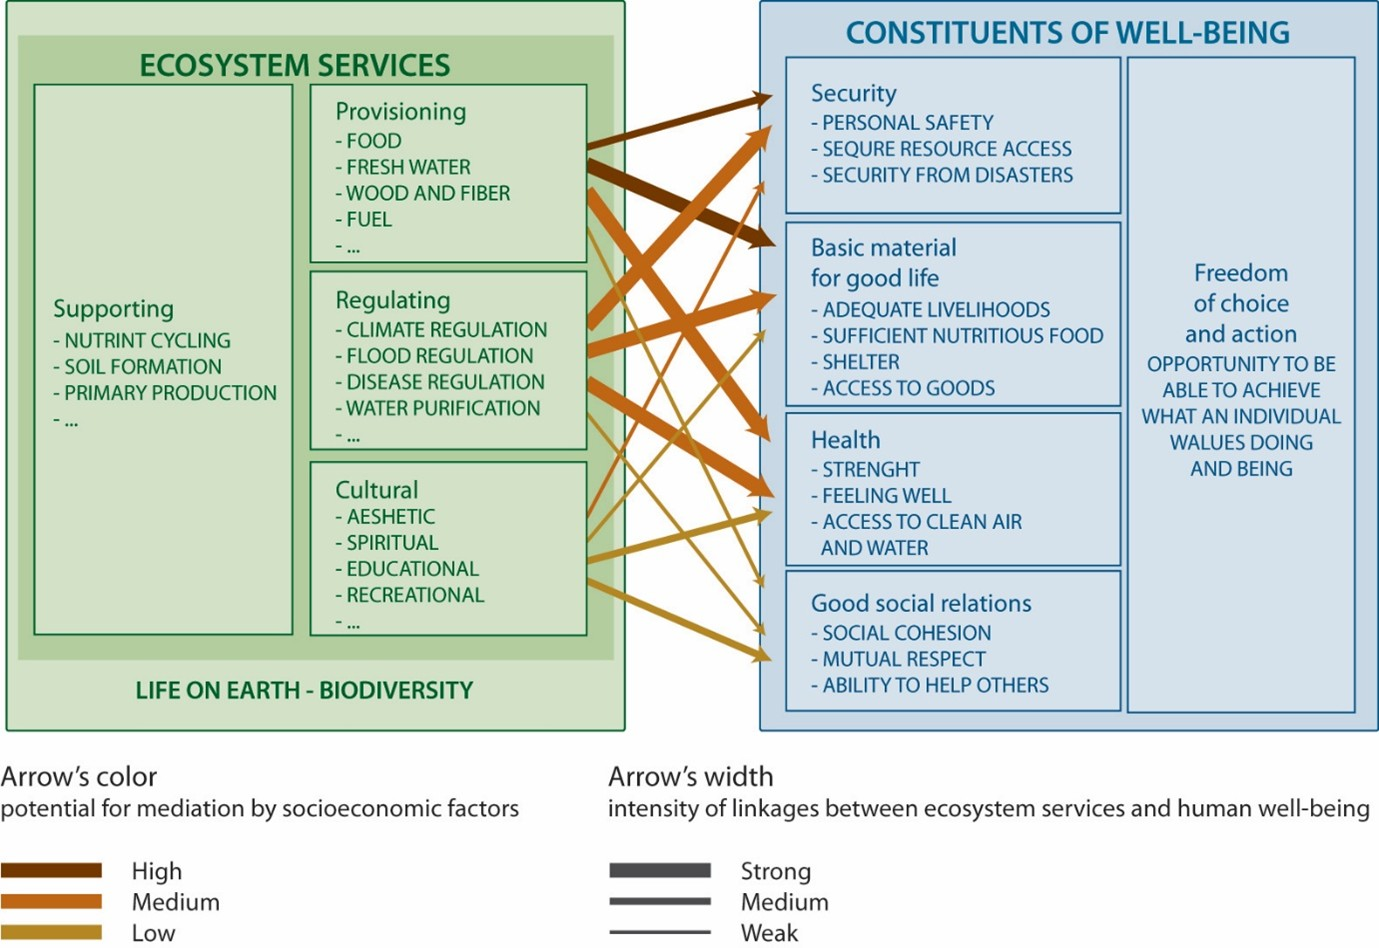
\includegraphics[keepaspectratio]{3_ecological-sustainability/images/Fig3_2__Ecosystem.jpg}}

}

\caption{\label{fig-ecosystem}Millennium Ecosystem Assessment. Quelle:
Millenium Ecosystem Assessment (2005). Lizenziert unter CC.}

\end{figure}%

Laut Millenium Ecosystem Assessment (2005) können diese
Ökosystemdienstleistungen unsere Lebensqualität und unsere Wirtschaft
verbessern (vgl. blauer Kasten in Abbildung~\ref{fig-ecosystem}). Diese
Betrachtungsweise von Ökosystemen sieht den Menschen zwar als von der
Umwelt getrennt, betont aber die Relevanz von Ökosystemdienstleistungen
für das menschliche Wohlergehen. Das Konzept der
Ökosystemdienstleistungen zielt letztlich darauf ab, den Wert der Natur
stärker in politische und wirtschaftliche Entscheidungen einzubeziehen.
Das Konzept spielt jedoch auch in der Landschafts- und Raumplanung eine
Rolle. Es wird beispielsweise genutzt, um zu analysieren, wie sich
räumlich wirksame (rechtliche) Regelungen auf Ökosystemdienstleistungen
und damit auf das menschliche Wohlergehen auswirken (vgl. {Albert u.~a.}
2016).

\begin{tcolorbox}[enhanced jigsaw, arc=.35mm, bottomrule=.15mm, bottomtitle=1mm, breakable, colback=white, colbacktitle=quarto-callout-tip-color!10!white, colframe=quarto-callout-tip-color-frame, coltitle=black, left=2mm, leftrule=.75mm, opacityback=0, opacitybacktitle=0.6, rightrule=.15mm, title={Fallstudie: Ökosystemdienstleistungen in Madagaskar}, titlerule=0mm, toprule=.15mm, toptitle=1mm]

Diese Landschaft an der Ostküste Madagaskars bietet eine Fallstudie für
Ökosystemdienstleistungen. Zu den Ökosystemdienstleistungen in diesem
Gebiet gehören Brennholz, das von der lokalen Bevölkerung zum Kochen
verwendet wird, und Reis, der ein Grundnahrungsmittel ist. Die
Bezeichnung landwirtschaftlicher Produkte wie dieser als
Ökosystemdienstleistungen verdeutlicht, dass sie erst durch menschliche
Nachfrage zu „Dienstleistungen'' werden. Ökosystemdienstleistungen sind
in der Natur nicht per se gegeben: Sie stellen vielmehr eine Perspektive
dar, durch die Menschen die Umwelt betrachten und beschreiben. Weitere
Ökosystemdienstleistungen in dieser Landschaft umfassen den
Wasserkreislauf, der für die lokale Bevölkerung lebenswichtig ist, da
sie auf Flüsse als Trinkwasserquelle angewiesen ist. Wasser wird auch
für die landwirtschaftliche Bewässerung und andere Zwecke genutzt. Die
Klimaregulierung ist eine weitere bedeutende Dienstleistung, die sowohl
lokal als auch global wichtig ist.

Diese Landschaft veranschaulicht klar, dass die Nachfrage nach
Ökosystemdienstleistungen und deren Bedeutung je nach Person oder Gruppe
variieren. Solche unterschiedlichen Ansprüche auf
Ökosystemdienstleistungen aus demselben Land können zu
\textbf{Interessenkonflikten} führen. Die Nachfrage nach
landwirtschaftlichen Produkten oder Brennholz kann beispielsweise mit
klimaregulierenden und biodiversitätsfördernden (internationalen)
Ansprüchen an den Regenwald in Konflikt geraten.

\end{tcolorbox}

Menschen haben viele Ökosystemdienstleistungen sowohl direkt als auch
indirekt beeinflusst. Während diese Auswirkungen oft negativ waren,
waren einige auch positiv. So hat beispielsweise die Ablösung
natürlicher Ökosysteme durch kultivierte Agrarökosysteme den Wert der
Ökosystemdienstleistungen für den Menschen erhöht. Nehmen wir als
Beispiel Trockenwiesen und Weiden in der Schweiz. Erst durch
jahrhundertelange Waldrodung und extensive landwirtschaftliche Nutzung
in alpinen Lagen konnten die von diesen Gebieten erbrachten
Ökosystemdienstleistungen (in diesem Fall die Futterproduktion) genutzt
und gesteigert werden. Gleichzeitig beherbergten diese anthropogen
beeinflussten Standorte seltene Wiesenpflanzen und Bestäuber und
förderten so ein hohes Mass an Biodiversität. Diese Gebiete sind auch
für den Tourismus von Bedeutung, da sie die alpine Landschaft
massgeblich prägen. Folglich bieten diese extensiv genutzten Flächen im
Allgemeinen eine grössere Multifunktionalität der
Ökosystemdienstleistungen als intensiv bewirtschaftetes Grünland
(Richter u.~a. 2024).

Viele der negativen Auswirkungen auf Ökosysteme und ihre
Dienstleistungen sind direkte Folgen menschlicher Landnutzung und
Überfischung. Darüber hinaus beeinträchtigen indirekte Faktoren wie der
Klimawandel und invasive gebietsfremde Arten die Stabilität und
Funktionsfähigkeit von Ökosystemen erheblich. Zwei Forschungsprojekte
mit massgeblicher CDE-Beteiligung -- Woody Weeds und Woody Weeds+ --
haben gezeigt, dass invasive Gehölze wie \emph{Prosopis juliflora} in
Ostafrika grosse Auswirkungen auf die Biodiversität und die lokalen
Lebensgrundlagen haben. Ursprünglich zur Bekämpfung von Wüstenbildung
und Holzeinschlag eingeführt, verdrängt diese Art die einheimische
Vegetation und ist ohne Verarbeitung nicht als Tierfutter geeignet
(\href{https://www.cde.unibe.ch/research/projects/woody_invasive_alien_species_in_eastern_africa/index_eng.html}{CDE-Projektwebsite}).

\subsection{Die monetäre Bewertung von
Ökosystemmanagement}\label{die-monetuxe4re-bewertung-von-uxf6kosystemmanagement}

Der Begriff \emph{Naturdienstleistungen} tauchte erstmals in der
Publikation „How much are Nature's Services Worth?'' (Westman 1977) auf.
Der synonym verwendete Begriff \emph{Ökosystemdienstleistungen} wurde
einige Jahre später geprägt (Ehrlich und Ehrlich 1981). Das Konzept der
Ökosystemdienstleistungen und das damit verbundene Denken sind eng mit
der Wirtschaftsphilosophie und -praxis verknüpft ({Gómez-Baggethun
u.~a.} 2010). Rund 20 Jahre nach der Einführung von
„Naturdienstleistungen'' schätzten Robert Costanza und Kolleg*innen,
dass der \textbf{globale Wert von 17 Ökosystemdienstleistungen 33
Billionen US-Dollar pro Jahr} betrage (Costanza u.~a. 1997). Eine
Neuberechnung im Jahr 2011 ergab, dass dieser Wert bereits um 4,3 bis
20,2 Billionen US-Dollar pro Jahr gesunken war (Costanza u.~a. 2014).
Bis 2050 wird vorhergesagt, dass der Wert der Ökosystemdienstleistungen
je nach Landnutzungsszenario entweder um bis zu 51 Billionen US-Dollar
pro Jahr sinken oder um bis zu 30 Billionen US-Dollar pro Jahr steigen
wird (Kubiszewski u.~a. 2017).

Die Berechnung des \textbf{monetären Werts von
Ökosystemdienstleistungen} umfasst typischerweise drei Schritte und
erfordert hochwertige und differenzierte Daten. 1) Im ersten Schritt
wird die Veränderung der Ökosystemdienstleistungen nach einer
Intervention gemessen; der Fokus liegt dabei nicht auf dem Status quo,
sondern auf der Differenz. 2) Im zweiten Schritt wird die Auswirkung
dieser Veränderung auf das sozioökonomische Wohlergehen der Menschen
bewertet. 3) Im dritten und letzten Schritt wird die resultierende
Veränderung der Produktivität oder des Wohlstands monetär bewertet. Es
gibt \textbf{viele verschiedene Methoden zur Berechnung des monetären
Werts von Ökosystemdienstleistungen}
(Abbildung~\ref{fig-monetary-value}). Eine davon ist das „grüne
Rechnungswesen'' (Green Accounting), das vorhandene Marktwerte, falls
verfügbar, oder Tauschwerte als Annäherung verwendet (z. B. Vergleich
von Lawinenbarrieren und Schutzwäldern). Eine weitere Methode ist die
Kosten-Nutzen-Analyse, die in zwei Typen unterteilt werden kann:
angegebene Präferenzen und offenbarte Präferenzen.

\begin{figure}[H]

\centering{

\pandocbounded{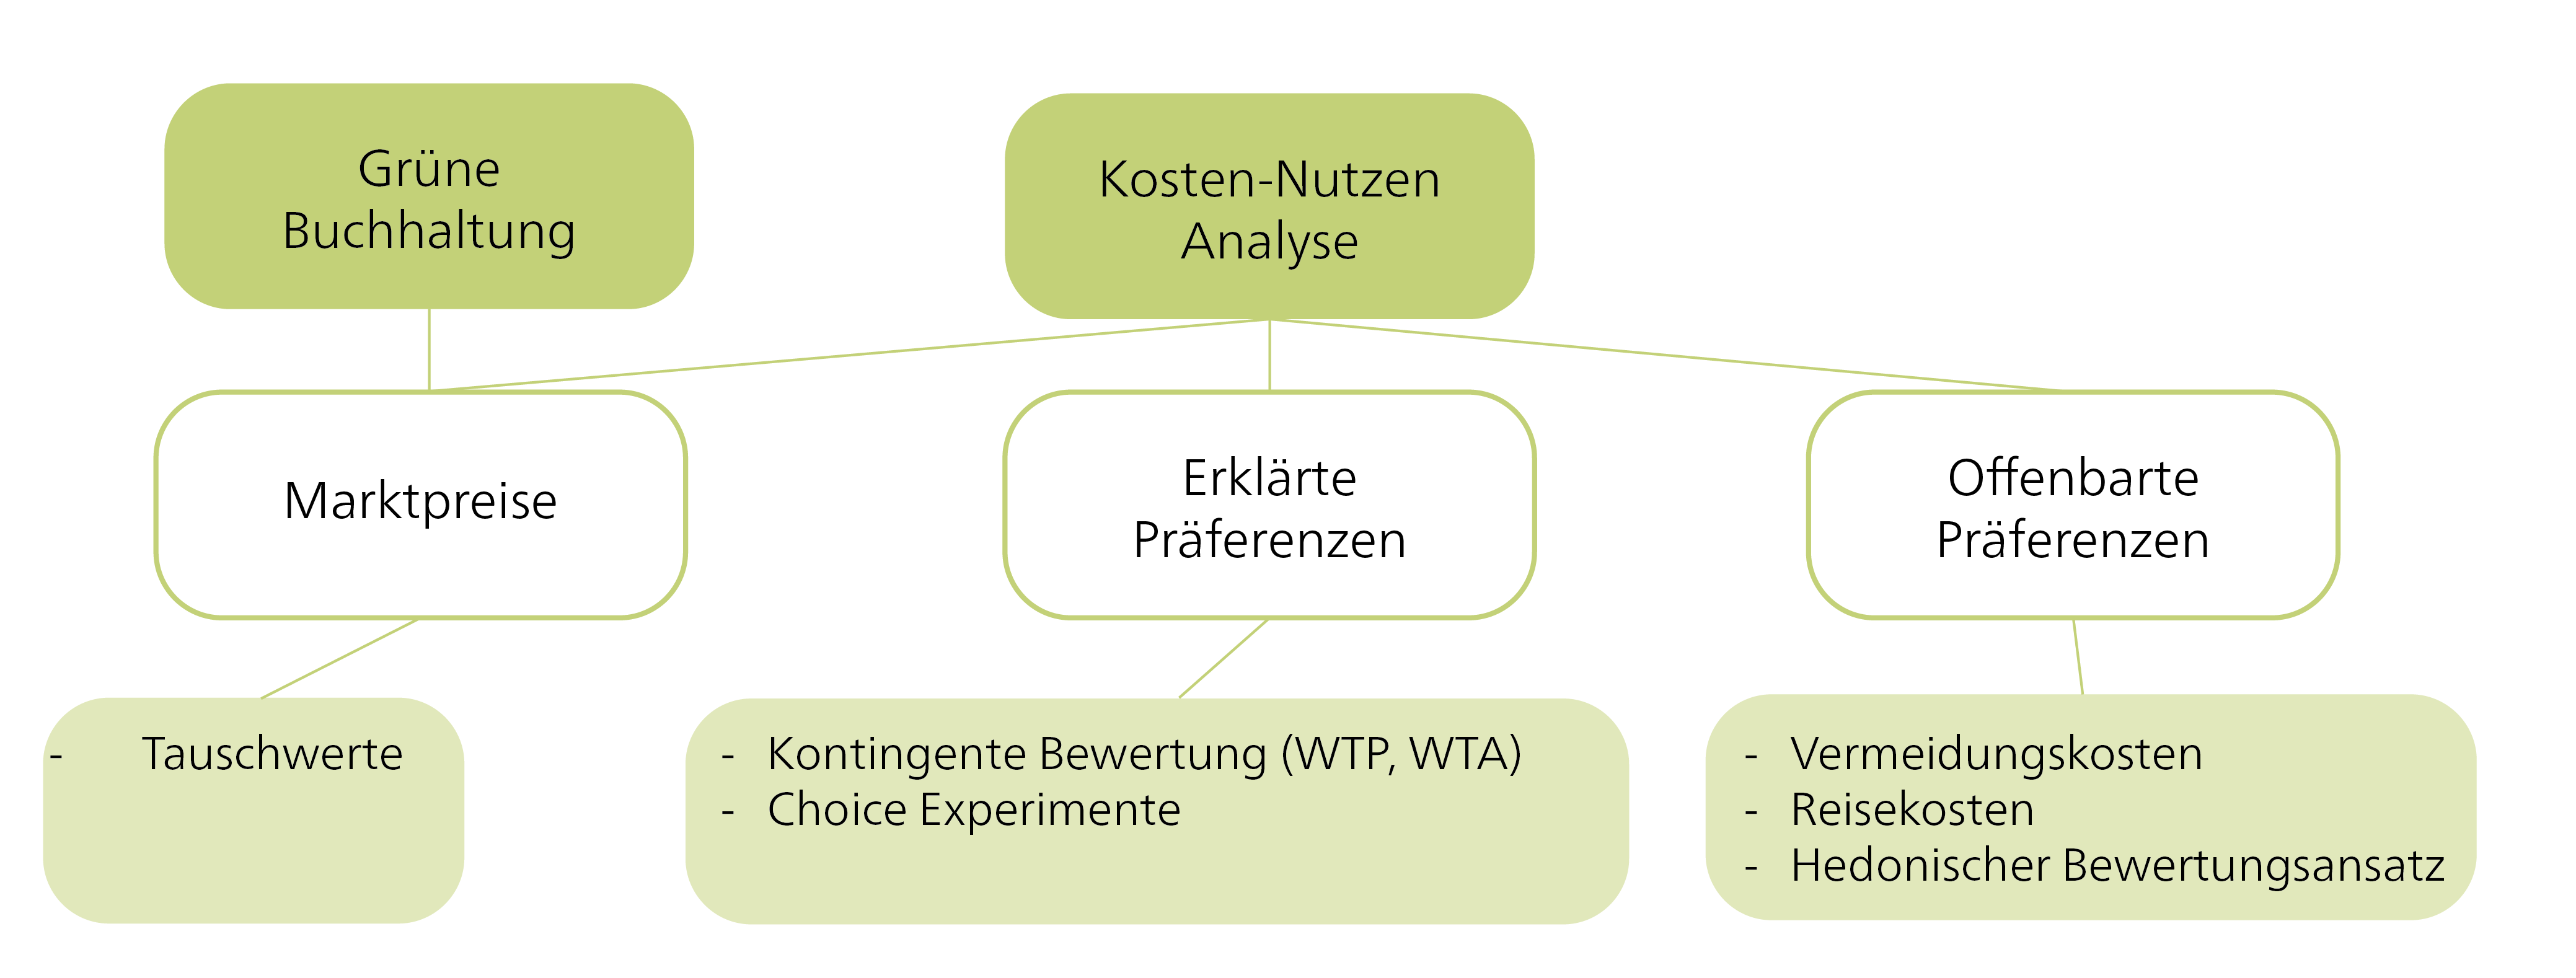
\includegraphics[keepaspectratio]{3_ecological-sustainability/images/Fig3_3__EcosystemValuation.png}}

}

\caption{\label{fig-monetary-value}Der monetäre Wert von
Ökosystemdienstleistungen. Quelle: Eigene Darstellung.}

\end{figure}%

Bei \textbf{angegebenen Präferenzen} geben Personen (z. B. in einer
Umfrage) an, inwieweit sie bereit wären, für bestimmte
Ökosystemdienstleistungen zu zahlen oder welche Veränderungen sie
akzeptieren würden (Kontingente Bewertung). Eine weitere Variante dieser
Methode beinhaltet die Wahl zwischen verschiedenen (meist suboptimalen)
Optionen, die jeweils einen Kompromiss auf der Grundlage von
Veränderungen der Ökosystemdienstleistungen darstellen (die dann
ökonometrisch analysiert werden). Im Gegensatz dazu basieren
\textbf{offenbarte Präferenzen} auf dem tatsächlichen Verhalten. Dabei
werden beispielsweise Vermeidungskosten analysiert (z. B. wie viel
Menschen für Lärmschutzwände bezahlen) oder Reisekosten berechnet (wobei
angenommen wird, dass der Zeit- und Reisekostenaufwand für den Besuch
eines Ortes den Wert des Ortes und damit im weiteren Sinne eine
Ökosystemdienstleistung widerspiegelt). Weitere Methoden umfassen
hedonische Ansätze, um zu bestimmen, inwieweit günstige oder ungünstige
Umwelteinflüsse und damit deren Qualität den Wert einer Immobilie
beeinflussen können.

Jede dieser Methoden hat ihre Vor- und Nachteile. Sie werden
hauptsächlich für ihre einseitigen Bewertungen und ihre mangelnde
Berücksichtigung sozialer Ungleichheiten, Machtverhältnisse und
kultureller Unterschiede kritisiert. Folglich sind diese Methoden nur
begrenzt in der Lage, faire und ökologisch nachhaltige Entscheidungen zu
fördern.

Das Prinzip hinter \textbf{Zahlungen für Ökosystemdienstleistungen
(Payments for Ecosystem Services, PES)} beinhaltet die Entschädigung von
Landnutzer*innen für die Aufrechterhaltung einer Komponente einer
bestimmten Ökosystemdienstleistung. Eine solche Entschädigung kann
beispielsweise von Organisationen oder Unternehmen gezahlt werden, für
die diese spezifischen Ökosystemdienstleistungen wichtig sind. Ein
bekanntes Beispiel für PES ist das Programm „Pagos por Servicios
Ambientales'' (PSA) in Costa Rica. Dieses seit 1997 laufende nationale
Programm wurde eingerichtet, um Entwaldung zu reduzieren und
Wiederaufforstung zu fördern, indem Grundeigentümer*innen dafür bezahlt
werden, Waldflächen zu erhalten, aufzuforsten oder nachhaltig zu
bewirtschaften. Die Zahlungen sollen die Bereitstellung von
Ökosystemdienstleistungen wie Kohlenstoffbindung, Wassererhalt,
Biodiversitätsschutz und Landschaftsschönheit fördern. Die Zahlungen in
diesem Projekt stammen aus verschiedenen Quellen, darunter eine
Kraftstoffsteuer und internationale Mittel von Organisationen, die an
CO\textsubscript{2}-Kompensation interessiert sind. Studien zeigen, dass
das Programm die Entwaldungsrate im Land erheblich reduziert und die
Erhaltung der Biodiversität gefördert hat, während gleichzeitig das
Einkommen der Grundeigentümer*innen gestiegen ist (Porras u.~a. 2013).

\subsection{Kritik an Ökosystemdienstleistungen und weitere sowie
alternative
Konzepte}\label{kritik-an-uxf6kosystemdienstleistungen-und-weitere-sowie-alternative-konzepte}

Das Konzept der Ökosystemdienstleistungen wurde zwar in der
wissenschaftlichen und politischen Debatte anerkannt und angewendet, es
wurde aber auch vielfach kritisiert (vgl. z. B. Kosoy und Corbera 2010;
Norgaard 2010). Ein Argument lautet, dass wir durch die Fokussierung auf
Ökosystemdienstleistungen die komplexen und vielfältigen Werte von
Ökosystemen auf ihren monetären Nutzen für den Menschen reduzieren (vgl.
{Schröter u.~a.} 2014). Diese \textbf{wirtschaftliche Reduktion der
Natur} vernachlässigt die nicht quantifizierbaren, aber dennoch
wichtigen Aspekte der Natur, wie spirituelle oder intrinsische Werte
(Fairhead u.~a. 2012). Die Kommodifizierung der Natur durch
Ökosystemdienstleistungen könnte letztlich auch zu einem ausbeuterischen
Verhältnis zwischen Mensch und Natur führen (vgl. {Schröter u.~a.} 2014)
oder \textbf{zu einer Verschärfung sozialer Ungleichheiten zwischen
mächtigen Akteuren und marginalisierten Gruppen} (Dawson u.~a. 2021), da
das Konzept Gerechtigkeit nicht explizit berücksichtigt (Loos u.~a.
2023, p.~478). In einigen Fällen wird sogar angenommen, dass das Konzept
der Ökosystemdienstleistungen mit dem Biodiversitätsschutz in Konflikt
geraten und ihn untergraben könnte (vgl. {Schröter u.~a.} 2014).

\begin{quote}
„Die Begeisterung für die Optimierung der Wirtschaft durch die
Einbeziehung von Ökosystemdienstleistungen hat uns für die wichtigere
Frage blind gemacht, wie wir die wesentlichen institutionellen
Veränderungen herbeiführen werden, um den menschlichen Druck auf
Ökosysteme erheblich zu reduzieren, insbesondere durch die Reichen, und
um uns anzupassen und effektiv mit den rasanten Ökosystemveränderungen
umzugehen, die durch bestehende und absehbare Klimadynamiken angetrieben
werden.'' (Norgaard 2010, p.~1220)
\end{quote}

Als Reaktion auf diese Kritik hat die Intergovernmental Platform on
Biodiversity and Ecosystem Services (IPBES) (vgl. Kapitel
\emph{Biodiversitätsverlust}) das Konzept der Ökosystemdienstleistungen
weiterentwickelt und ein weiteres Konzept entwickelt: das der
\emph{Naturbeiträge für Menschen} (Nature's Contributions to People,
NCP). NCPs werden definiert als „alle positiven Beiträge oder Vorteile
\emph{und} gelegentlich negativen Beiträge, Verluste oder Nachteile, die
Menschen aus der Natur gewinnen.'' ({Pascual u.~a.} 2017, p.~9). Das
Konzept ähnelt dem der Ökosystemdienstleistungen, geht aber weiter und
erkennt an, dass die Natur und ihre Beiträge zu einem guten Leben je
nach kulturellem und institutionellem Kontext unterschiedlich
wahrgenommen und betrachtet werden können. Das Konzept strebt die
Einbeziehung verschiedener Weltanschauungen an, wie z. B. indigener
Wissenssysteme, und berücksichtigt damit sowohl intrinsische (d.~h.
nicht-anthropozentrische) als auch relationale Werte der Natur ({Díaz
u.~a.} 2018). Insgesamt berücksichtigt dieser Ansatz auch
kontextspezifische Perspektiven und gibt Gerechtigkeitsdimensionen
stärker Rechnung als das Konzept der Ökosystemdienstleistungen (Loos
u.~a. 2023).

Jedoch sind auch solche \textbf{pluralen Bewertungen} nicht ohne Kritik
und stellen verschiedene Herausforderungen dar. So weisen Jacobs u.~a.
(2023) darauf hin, dass aktuelle Ansätze zur Integration mehrerer Werte
und Perspektiven in Ökosystembewertungen das Risiko bergen, lediglich
Pseudo-Partizipation zu fördern, während bestehende \textbf{Macht- und
Diskriminierungsstrukturen} unverändert bleiben. Plurale Bewertungen
streben Inklusivität und Demokratie an, können jedoch bei unzureichender
Gestaltung unbeabsichtigt zu Konflikten, Machtungleichgewichten und
unklaren Ergebnissen führen. Wissenschaftler*innen haben auch das oben
erwähnte NCP-Konzept kritisiert, das oft als unzureichende
Weiterentwicklung des \textbf{utilitaristischen Umweltschutzes}
angesehen wird. Dabei handelt es sich um eine stark westliche und
anthropozentrische Perspektive, die eine dualistische Trennung von
Mensch und Natur aufrechterhält (vgl. Muradian und Gómez-Baggethun
2021). Muradian und Gómez-Baggethun (2021) {[}p.~7{]} schlagen vor, dass
„um transformativen Wandel in den Mensch-Natur-Beziehungen
herbeizuführen, wir einen Wechsel von einer Moral der Nützlichkeit zu
einer Moral der Fürsorge, eine Neuverteilung von Eigentumsrechten und
die Ausdehnung der Gerechtigkeitsgemeinschaft auf nicht-menschliche
Entitäten brauchen.'' Ein bemerkenswertes Beispiel für diese
Transformation ist die Anerkennung des Whanganui-Flusses in Neuseeland
als juristische Person im Jahr 2017 (vgl. Charpleix 2018).

\section{Planetare Grenzen}\label{planetare-grenzen}

Die gegenwärtige Epoche wird als Anthropozän bezeichnet, weil
menschliche Aktivitäten einen immer tiefgreifenderen Einfluss auf die
Erde und ihre Systeme ausüben. Obwohl dieser Begriff von geologischen
Fachgremien (noch) nicht als offizielle geologische oder
geochronologische Epoche anerkannt wurde (Zhong 2024), beschreibt er den
enormen menschlichen Einfluss auf die Umwelt. Es gibt keine einheitliche
Definition über den Ursprung des Anthropozäns; mögliche Marker umfassen
den menschlichen Einfluss auf Treibhausgaskonzentrationen durch den
Reisanbau, die globale Verbreitung von Radioaktivität durch Atomtests
oder das Auftreten von Kunststoffpartikeln in geologischen Sedimenten.
Als Beginn des Anthropozäns gilt allgemein die Industrielle Revolution.

Eine quantitative Definition ökologischer Nachhaltigkeit wurde von
{Rockström, Steffen, Noone, Persson, F. S. I. Chapin, u.~a.} (2009) und
{Steffen u.~a.} (2015) vorgeschlagen, die neun planetare Grenzen
identifizierten: Klimawandel, Integrität der Biosphäre,
Landnutzungsveränderungen, Süsswasserveränderungen, biogeochemische
Kreisläufe, Ozeanversauerung, atmosphärische Aerosollast,
stratosphärischer Ozonabbau sowie neuartige Stoffe. Diese planetaren
Grenzen dienen als wissenschaftlicher Referenzpunkt und zeigen die
Grenzen auf, innerhalb derer unsere globalen sozioökonomischen Systeme
operieren müssen, um das Wohlergehen der Menschheit zu gewährleisten.

Dieses Kapitel konzentriert sich auf drei dieser Grenzen, die hier als
\textbf{Klimawandel}, \textbf{Landnutzungsveränderungen} und
\textbf{Biodiversitätsverlust} bezeichnet werden. Diese drei Krisen
verstärken sich gegenseitig und bilden ein komplexes Geflecht von
Wechselwirkungen.

\begin{figure}[H]

\centering{

\pandocbounded{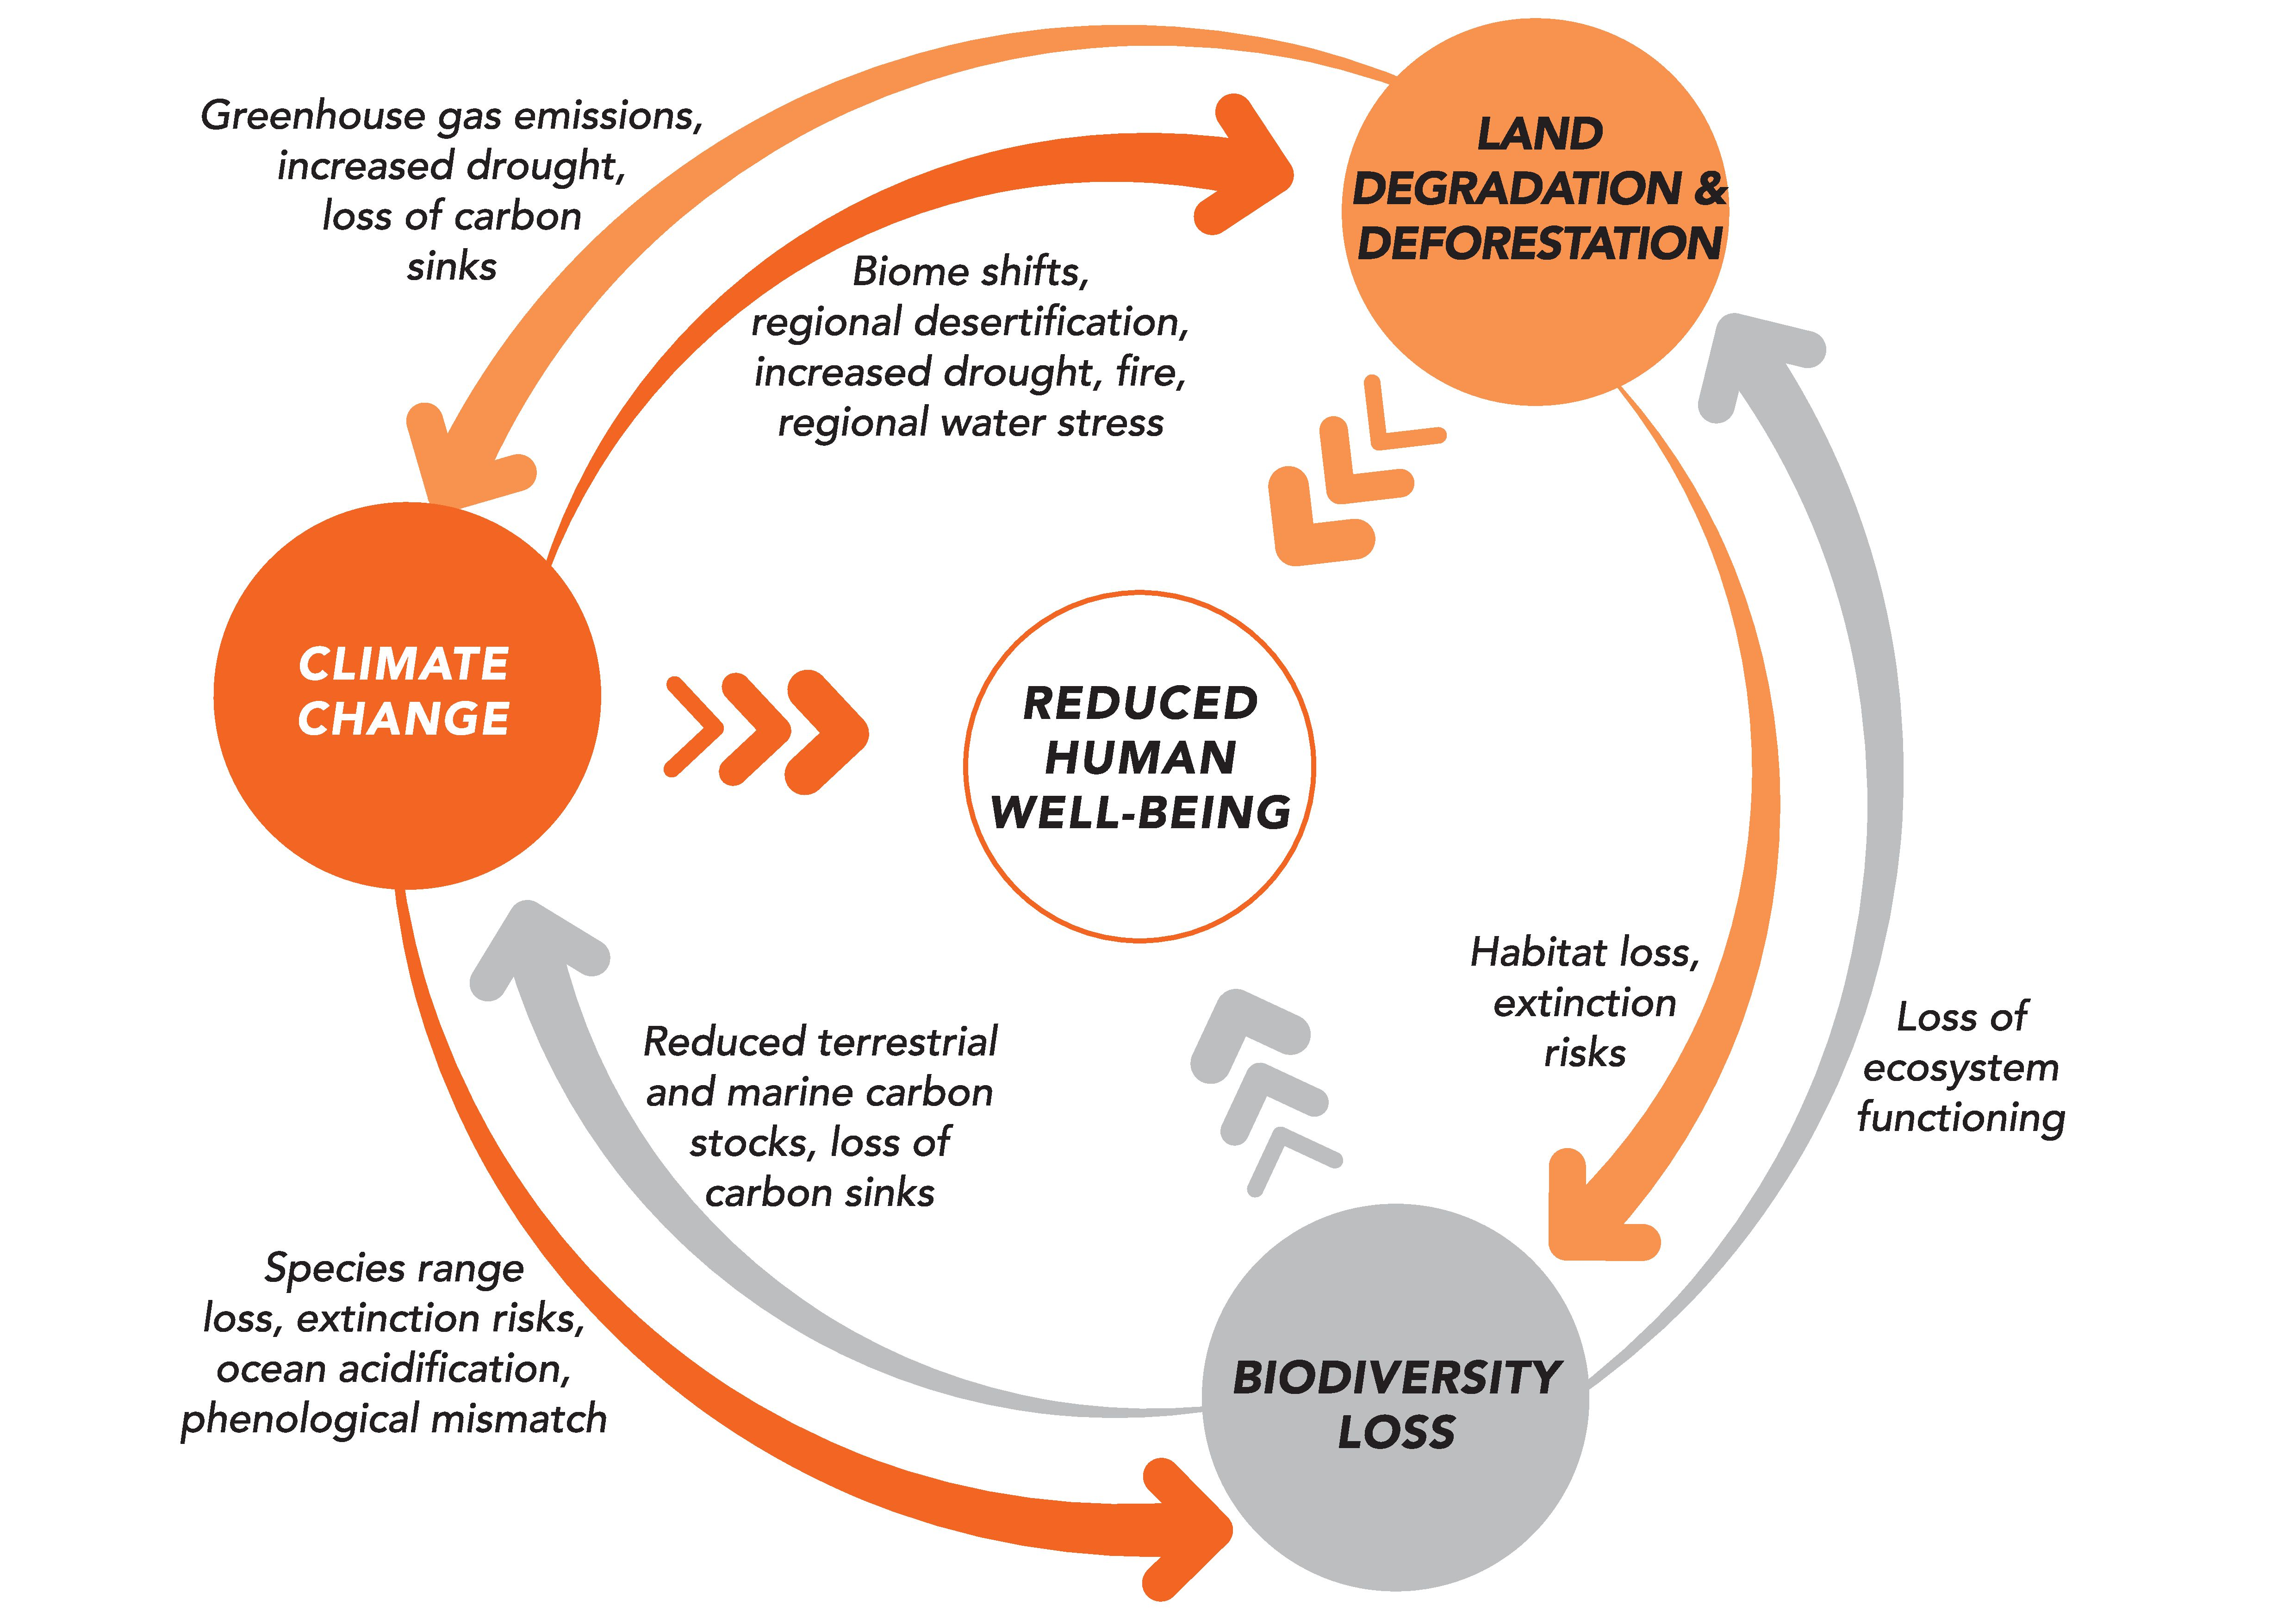
\includegraphics[keepaspectratio]{3_ecological-sustainability/images/Fig3_4_LandClimateBiodiversity.jpg}}

}

\caption{\label{fig-interactions}Interaktionen zwischen Biodiversität,
Klimawandel und Landnutzung. Quelle: UNEP (2021). Lizenziert unter
CC-BY.}

\end{figure}%

\subsection{Die Klimakrise
(Klimawandel)}\label{die-klimakrise-klimawandel}

\textbf{Klimawandel} -- oder, um einen Begriff zu verwenden, der die
Dringlichkeit besser verdeutlicht, die Klimakrise -- ist eines der
drängendsten Probleme unserer Zeit. Er erfährt grosse mediale
Aufmerksamkeit und ist beispielhaft für ein „wicked problem'' (Hulme
2009, p.9). Er steht im Mittelpunkt der Fridays-for-Future-Bewegung, die
von Greta Thunberg initiiert wurde, und ist zumindest ein Gesprächsthema
auf der (globalen) politischen Bühne. Während lokale Bedingungen und
natürliche Schwankungen zu gewissen Unsicherheiten in Klimamodellen und
Statistiken beitragen, zeigt die wissenschaftliche Evidenz klar, dass
steigende globale Temperaturen einen enormen Einfluss auf die
ökologische Nachhaltigkeit und das menschliche Wohlergehen haben.
Deshalb ist der Klimawandel eine der neun planetaren Grenzen.

Der Begriff \textbf{Klima} beschreibt den durchschnittlichen Zustand der
Atmosphäre (Temperatur, Niederschlag, Luftfeuchtigkeit usw.) über einen
Zeitraum von mindestens 30 Jahren an einem bestimmten Ort. Im Gegensatz
dazu beschreibt \textbf{Wetter} den kurzfristigen Zustand (d.~h. von
Sekunden bis Wochen) und umfasst Wetterphänomene wie Gewitter oder
Hitzewellen (NCCS, o.~J.). Das \textbf{Klimasystem} wiederum umfasst
nicht nur die Atmosphäre, sondern auch die Hydrosphäre (Ozeane, Seen,
Flüsse, Grundwasser), die Kryosphäre (Gletscher, Schneedecke, Meeres-
und Seeeis, Permafrost), die Biosphäre (Lebewesen) und die Lithosphäre
(Böden bzw. die äusserste Schicht der Erde). Es bezeichnet insbesondere
die physikalischen, biologischen und chemischen Wechselwirkungen und
Abhängigkeiten zwischen diesen fünf Sphären. Zusätzlich wird das
Klimasystem durch Strahlung aus dem Weltraum beeinflusst (vgl. Abbildung
unten).

\begin{figure}[H]

\centering{

\pandocbounded{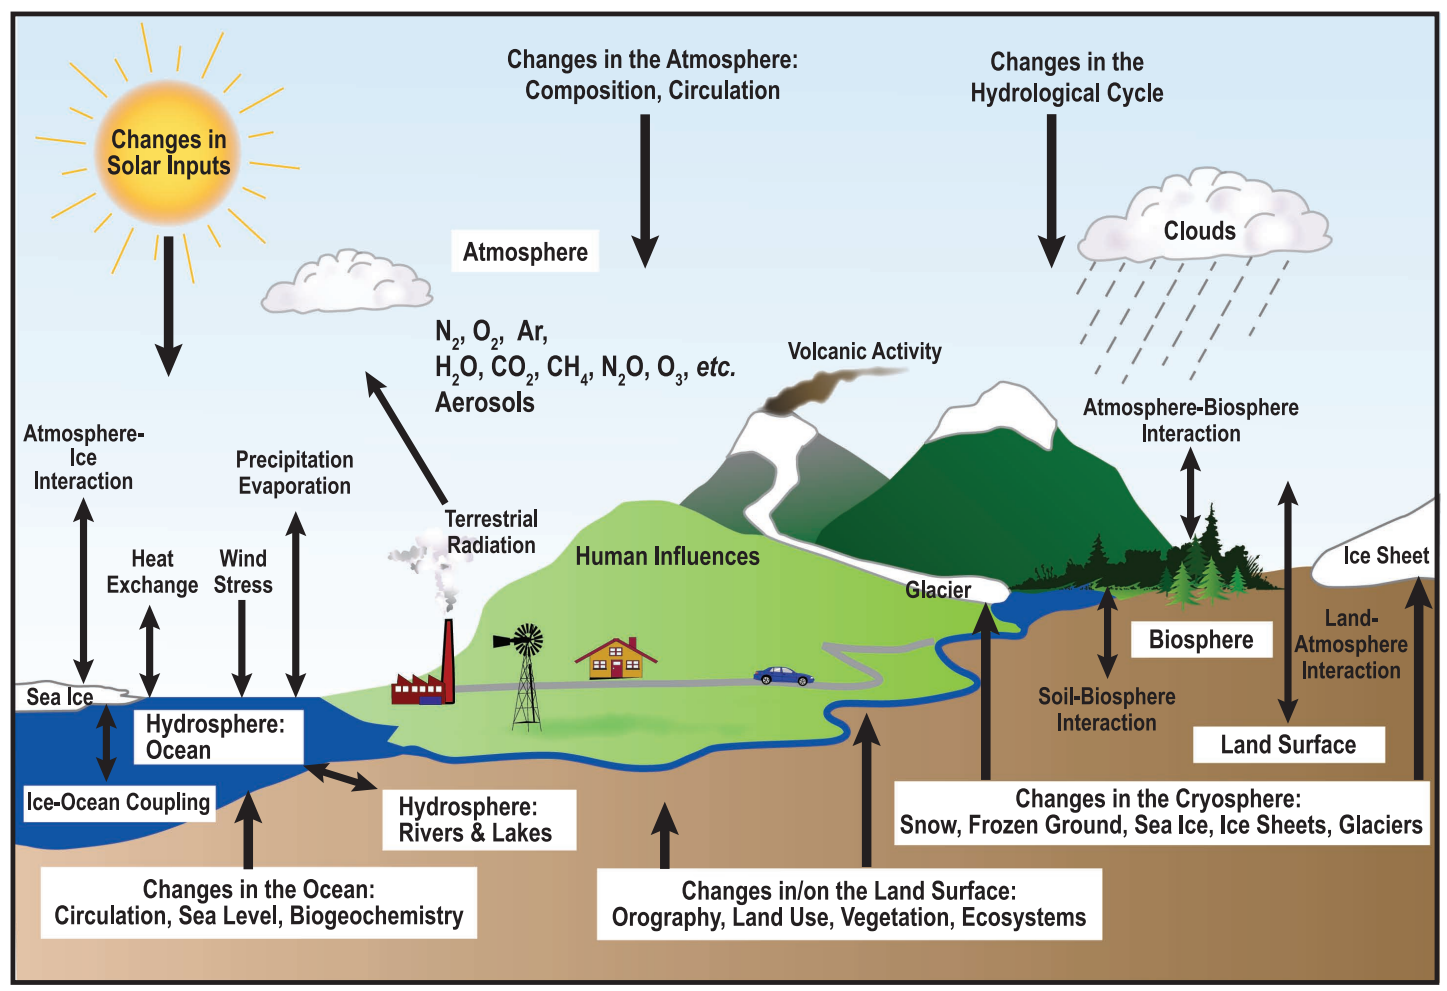
\includegraphics[keepaspectratio]{3_ecological-sustainability/images/Fig3_5_ClimateSystem.png}}

}

\caption{\label{fig-climate-system}Die Komponenten des Klimasystems,
ihre Prozesse und Wechselwirkungen. Dies umfasst die Atmosphäre,
Biosphäre (Leben), Kryosphäre (Eis), Hydrosphäre (Wasser), Land und
menschliche Einflüsse sowie die Wechselwirkungen zwischen diesen
Komponenten (mit doppelten Pfeilen dargestellt). Die Teile des Systems,
die sich verändern können, sind als „Changes'' (Veränderungen)
beschriftet. Quelle: IPCC AR4 FAQ
(\url{https://archive.ipcc.ch/publications_and_data/ar4/wg1/en/faq-1-2.html}).}

\end{figure}%

Material- und Energieflüsse zwischen den verschiedenen Komponenten des
Klimasystems, wie der Kohlenstoffkreislauf, können als
\textbf{Rückkopplungsmechanismen} wirken. Solche
Rückkopplungsmechanismen haben wir bereits im Kapitel über systemische
Effekte kennengelernt (vgl. \emph{Kapitel 2}). Sie können entweder
positiv sein, wenn die Rückkopplung die ursprüngliche Veränderung
verstärkt, oder negativ, wenn die Rückkopplung versucht, die
ursprüngliche Veränderung umzukehren. Hier sind Beispiele für einen
positiven und einen negativen Rückkopplungseffekt im Klimasystem:

\begin{itemize}
\item
  \textbf{Positive Rückkopplung}: Wenn die Erdoberflächentemperatur
  steigt, nimmt auch die Wasserverdunstung zu, was eine positive
  Rückkopplungsschleife erzeugt. Wasserdampf ist das bedeutendste
  \textbf{Treibhausgas} in der Atmosphäre. Mit steigenden Temperaturen
  gelangt mehr Wasserdampf in die Atmosphäre, was die Wärmereflexion zur
  Erdoberfläche verstärkt und zu weiterer Verdunstung führt. Dieser
  Kreislauf beschleunigt die Erwärmung und die Ansammlung von
  atmosphärischem Wasserdampf. Auf der Venus verstärkte dieser
  Rückkopplungsmechanismus den Treibhauseffekt so weit, dass alles
  flüssige Oberflächenwasser verdampfte.
\item
  \textbf{Negative Rückkopplung}: Erhöhtes atmosphärisches
  CO\textsubscript{2} kann die Photosynthese fördern, ein Prozess, der
  als \textbf{CO\textsubscript{2}-Düngungseffekt} bekannt ist und ein
  Beispiel für einen negativen Rückkopplungsmechanismus darstellt.
  Obwohl ein Anstieg des Kohlendioxids dazu führen kann, dass Pflanzen
  mehr Kohlenstoff in Biomasse binden als zuvor, reicht dies bei weitem
  nicht aus, um den steigenden CO\textsubscript{2}-Gehalt in der
  Atmosphäre zu kompensieren, der hauptsächlich durch die Verbrennung
  fossiler Brennstoffe und Landnutzungsveränderungen verursacht wird.
  Die Fähigkeit der Pflanzen, zusätzliches CO\textsubscript{2}
  aufzunehmen, wird durch verschiedene Faktoren wie
  Nährstoffverfügbarkeit, Wasserressourcen und Temperaturbedingungen
  begrenzt. Daher ist dieser Rückkopplungsmechanismus unzureichend, um
  den Anstieg der atmosphärischen CO\textsubscript{2}-Konzentration
  durch menschliche Aktivitäten zu kompensieren.
\end{itemize}

Positive Rückkopplungsmechanismen oder das Versagen negativer
Rückkopplung können dazu führen, dass bedeutende \emph{Schwellenwerte}
im Klimasystem überschritten werden. Diese Schwellenwerte werden als
\textbf{Kipppunkte des Klimasystems} bezeichnet und sind eng mit dem
Konzept der planetaren Grenzen verknüpft (vgl. \emph{Kapitel 2.4 zur
Grossen Transformation}). Wenn diese Schwellenwerte überschritten
werden, können abrupte und oft irreversible Veränderungen im Klimasystem
auftreten, die das Klima destabilisieren und zu einem beschleunigten
Klimawandel führen. Das Konzept der Kipppunkte unterstreicht die
Dringlichkeit, die globale Erwärmung zu begrenzen und
Treibhausgasemissionen zu reduzieren. Werden diese Schwellenwerte
überschritten, wird es zunehmend schwieriger, den Klimawandel zu
kontrollieren oder seine Auswirkungen zu minimieren. Letztlich riskiert
die Erde, zu einem grossen Treibhaus zu werden (\emph{Hothouse
Earth}-Szenario) (vgl. Abbildung~\ref{fig-hothouse-earth}).

\begin{figure}[H]

\centering{

\pandocbounded{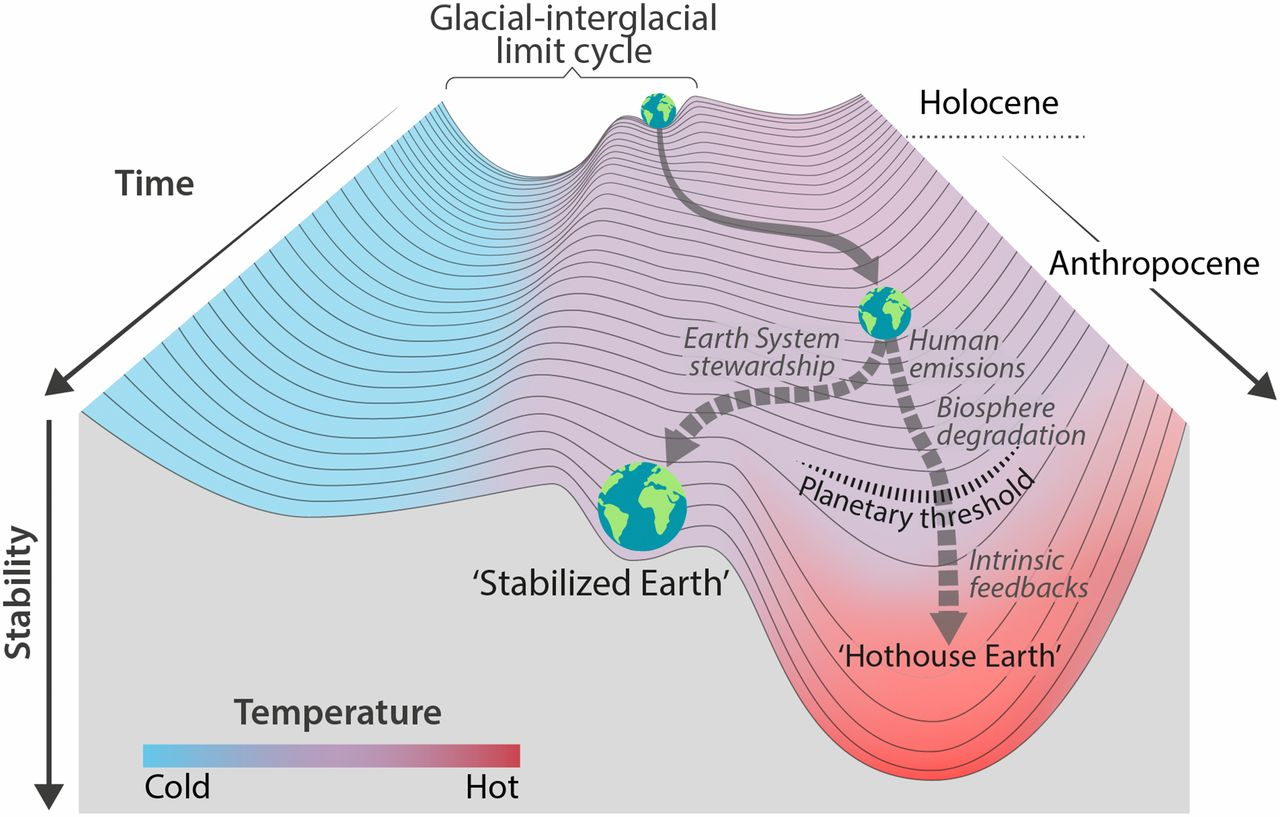
\includegraphics[keepaspectratio]{3_ecological-sustainability/images/Fig3_6__HothouseEarth.jpeg}}

}

\caption{\label{fig-hothouse-earth}Stabilitätslandschaft, die den Weg
des Erdsystems aus dem Holozän und damit aus dem glazial-interglazialen
Grenzzyklus in seine gegenwärtige Position im heisseren Anthropozän
zeigt. Quelle: Steffen u.~a. (2018). Lizenziert unter CC BY-NC-ND 4.0.}

\end{figure}%

Es wird angenommen, dass insgesamt 16 Kipppunkte existieren
(Abbildung~\ref{fig-16-tipping-points}), darunter die sibirischen
Permafrostböden oder der Westantarktische Eisschild. Diese Kipppunkte
haben unterschiedliche Schwellenwerte, was bedeutet, dass einige früher
-- bei geringerer globaler Erwärmung -- erreicht werden als andere. Wenn
diese Kipppunkte erreicht oder überschritten werden, können sie
selbstverstärkende Rückkopplungseffekte auslösen, die zu weiterer
Erwärmung führen, weitere Kipppunkte initiieren und den Klimawandel
intensivieren. Einige dieser Kipppunkte befinden sich bereits in einem
kritischen Zustand, wie Johan Rockström, einer der Begründer des
Konzepts der Planetaren Grenzen, eindrücklich erklärt (Rockström 2024).
Im Amazonas beispielsweise emittieren einige Gebiete mittlerweile mehr
CO\textsubscript{2} als sie absorbieren -- sie werden zu
Kohlenstoff\emph{quellen} statt zu -senken -- aufgrund von Waldbränden,
klimabedingtem Wasserstress und Entwaldung (vgl. \emph{Kapitel 3.3.2 zu
Landnutzungsveränderungen}) (Gatti u.~a. 2021; {Harris u.~a.} 2021).
Folglich befindet sich der Amazonas bereits im Wandel und verliert an
Resilienz ({Flores u.~a.} 2024). Ein weiterer besorgniserregender und
sehr realer Kipppunkt ist die \emph{Atlantische Umwälzzirkulation}
(Atlantic Meridional Overturning Circulation, AMOC) (Rahmstorf 2024a,
2024b). Die AMOC nähert sich ihrem Kipppunkt ({van Westen u.~a.} 2024),
und Projektionen deuten darauf hin, dass sie schon Mitte dieses
Jahrhunderts kollabieren könnte (Ditlevsen und Ditlevsen 2023). Ein
Kollaps würde zu häufigeren europäischen Hitzewellen und einem
Meeresspiegelanstieg entlang der nordöstlichen US-Küste führen
(Rahmstorf 2024a).

\begin{figure}[H]

\centering{

\pandocbounded{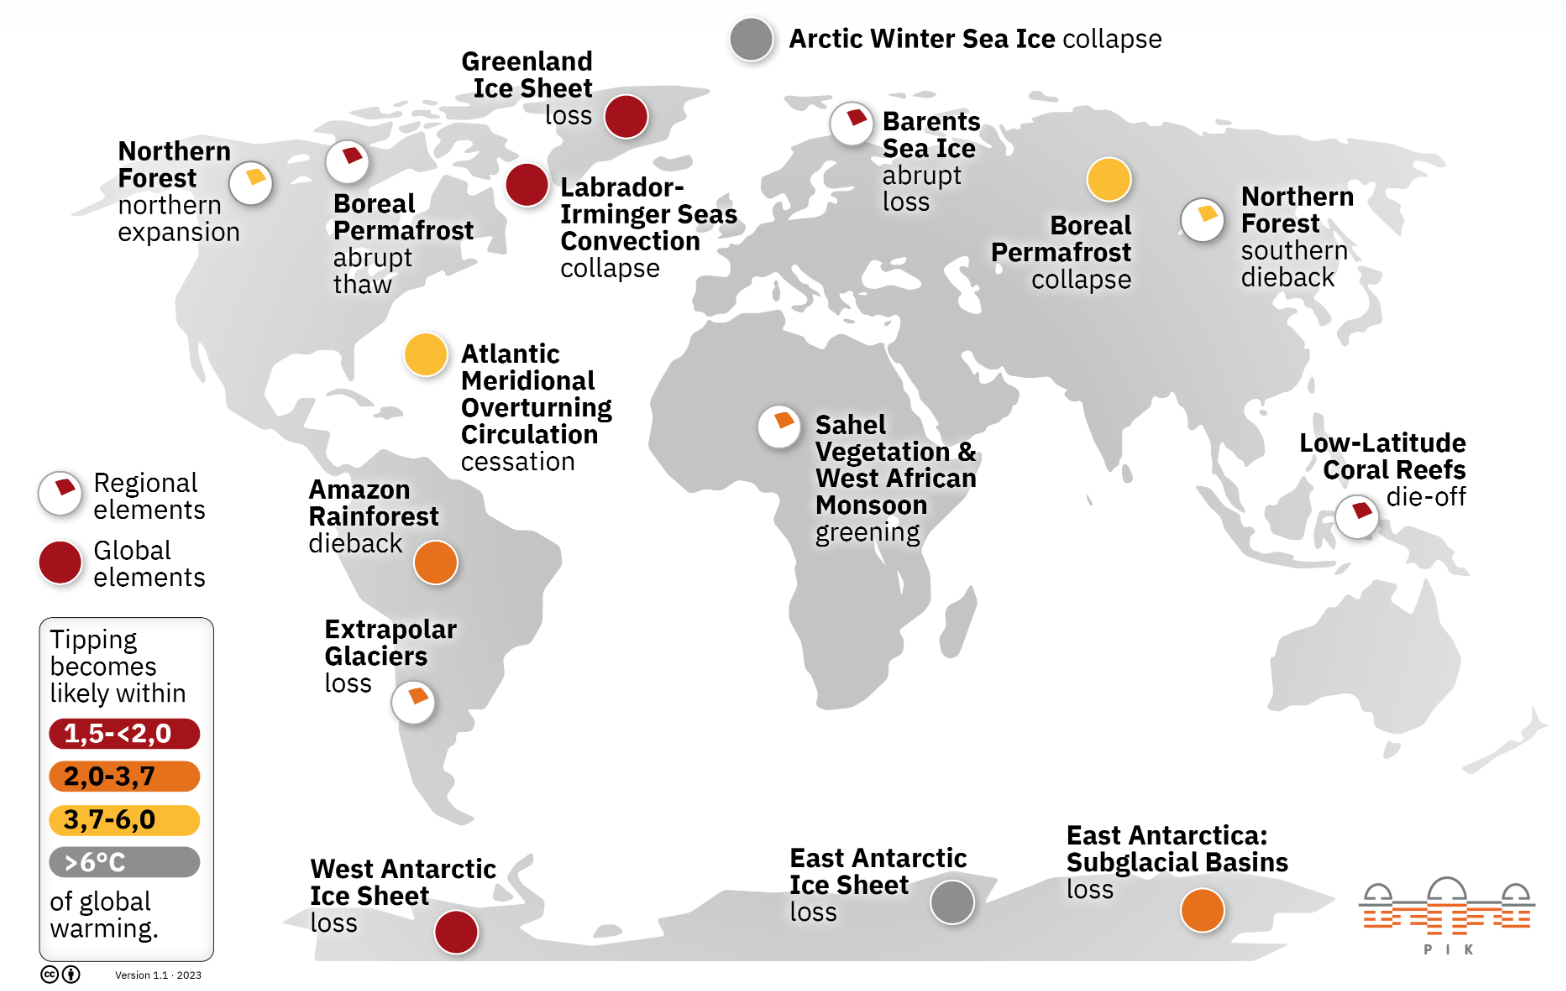
\includegraphics[keepaspectratio]{3_ecological-sustainability/images/Fig3_7__tippingpoints.png}}

}

\caption{\label{fig-16-tipping-points}Räumliche Verteilung globaler und
regionaler Kipppunkte. Die Farben geben die Temperaturbandbreite an, in
der ein Kippen wahrscheinlich ist. Quelle: Erstellt am PIK, basierend
auf Armstrong McKay u.~a. (2022), ergänzt mit Interaktionen nach Lenton
u.~a. (2019). Lizenziert unter CC-BY.}

\end{figure}%

Doch was verursacht die Erwärmung der Erde und den Klimawandel? Neben
natürlichen Ursachen wie geologischen, langfristigen Faktoren
(Erdachsenrotation, Milanković-Zyklen, Vulkanausbrüche) ist der primäre
Treiber der globalen Erwärmung der \textbf{Treibhausgaseffekt}. Der
Treibhausgaseffekt ist ein Prozess, bei dem kurzwellige Sonnenstrahlung
in die Erdatmosphäre eindringt und von der Erdoberfläche als langwellige
Infrarotstrahlung wieder abgestrahlt wird. Treibhausgase -- wie
Kohlendioxid, Methan und Wasserdampf -- absorbieren einen Teil dieser
Infrarotstrahlung und emittieren sie in alle Richtungen, wodurch ein
Teil der Wärme zur Erdoberfläche zurückgelangt. Ohne diesen Effekt wäre
die Erde zu kalt, um Leben zu ermöglichen. Heute befinden sich jedoch
aufgrund anthropogener Emissionen zu viele Treibhausgase in der
Atmosphäre, was zur Erwärmung der Erde führt.

Der grösste Anteil der menschlichen CO\textsubscript{2}-Emissionen, rund
¾ des globalen Gesamtvolumens, stammt aus der Energieproduktion, d.~h.
in erster Linie aus der Strom- und Wärmeerzeugung
(Abbildung~\ref{fig-global-greenhouse-gas-emissions}). Dies ist
hauptsächlich auf die Verbrennung von Kohle, Gas und Öl zurückzuführen,
mit Emissionen aus Industrie (24,2\% des globalen Gesamtvolumens),
Transport (16,2\%), Gebäuden (17,5\%) und Landwirtschaft (18,4\%). Die
Haupttreiber der landwirtschaftlichen Emissionen sind die Viehzucht, die
Entwaldung für landwirtschaftliche Nutzflächen und der Einsatz von
Stickstoffdünger auf landwirtschaftlichen Böden.

Im Transportsektor macht der Luftverkehr 1,9\% der globalen Emissionen
aus (vgl. Abbildung unten). In der Schweiz hingegen entfallen auf Flüge
rund 11\% der nationalen Emissionen. Diese Flugverkehrsemissionen sind
grösstenteils dem internationalen Luftverkehr zuzuschreiben (FOEN 2025),
wobei der Flughafen Basel-Mulhouse, der sich auf französischem Boden
befindet, nicht in die Berechnungen einfliesst. Trotz dieser Evidenz hat
die Schweiz noch keine CO\textsubscript{2}-Steuer auf Kerosin (den
Hauptbestandteil des Flugzeugtreibstoffs) eingeführt, obwohl eine solche
auf fossile Brennstoffe wie Heizöl und Erdgas besteht. Es ist jedoch
anzumerken, dass die Klimawirkung nicht allein durch
Treibhausgasemissionen bestimmt wird (Allen u.~a. 2018; Lee u.~a. 2021;
Neu 2021). Das Erwärmungspotenzial des Flugverkehrs kann daher deutlich
höher sein als durch die Treibhausgasemissionen allein angezeigt wird,
da auch Nicht-CO\textsubscript{2}-Effekte von Flügen -- wie Wasserdampf,
Stickoxide (NOx) und Russ -- das Klima beeinflussen (Lee u.~a. 2021).

Global haben die Flugverkehrsemissionen seit 1990 mehr als verdoppelt,
getrieben hauptsächlich durch den internationalen Luftverkehr. Trotz
eines starken Einbruchs der Flugzahlen im Jahr 2020 infolge der Pandemie
haben sich die Flugverkehrsemissionen erholt und werden voraussichtlich
in den kommenden Jahren die Rekordzahlen von 2019 übertreffen.

\begin{figure}[H]

\centering{

\pandocbounded{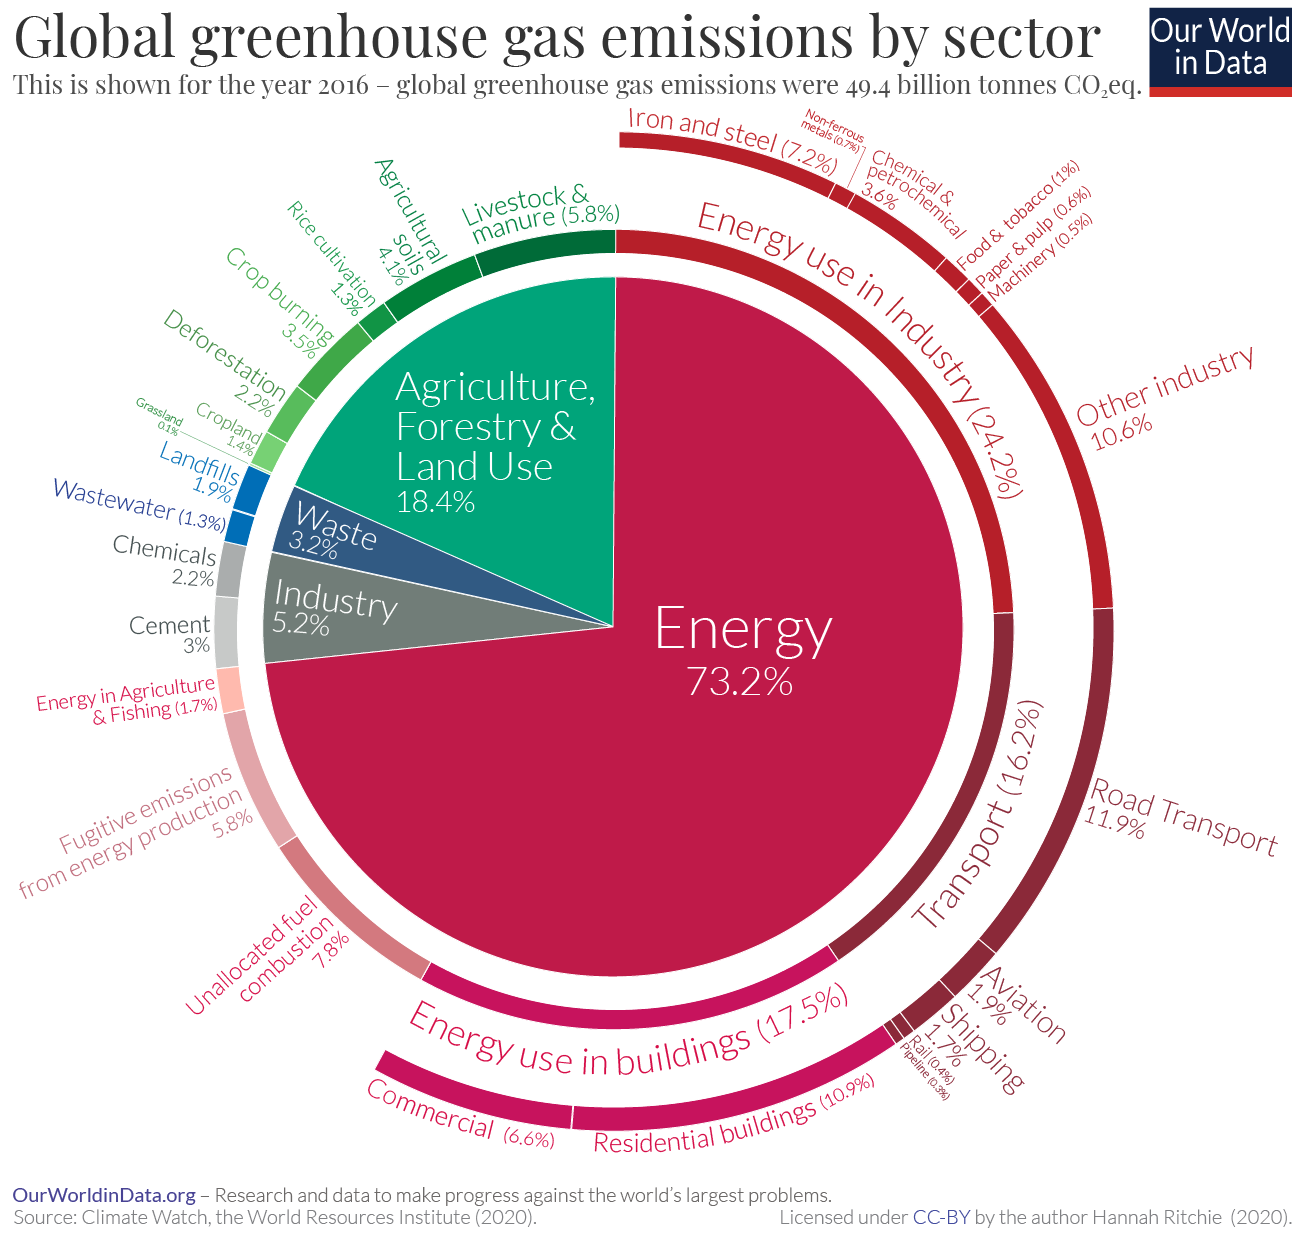
\includegraphics[keepaspectratio]{3_ecological-sustainability/images/Fig3_8__GreenhouseSector.png}}

}

\caption{\label{fig-global-greenhouse-gas-emissions}Globale
Treibhausgasemissionen nach Sektor. Quelle:
\url{https://ourworldindata.org/ghg-emissions-by-sector}.}

\end{figure}%

Jüngste Berechnungen und Klimaberichte zeigen, dass die
Erdoberflächentemperatur in den letzten 10 Jahren (2014--2023) im
Vergleich zum vorindustriellen Niveau (1850--1900) um rund 1,2°C
gestiegen ist (UN 2024). Zudem war 2023 das wärmste Jahr seit Beginn der
Aufzeichnungen, mit einer globalen Oberflächentemperatur von 1,45°C über
dem vorindustriellen Referenzwert. Das mag nicht viel klingen, bedeutet
aber angesichts der enormen Grösse und Wärmespeicherkapazität der Ozeane
einen erheblichen Wärmeanstieg (Ritchie 2020).

\begin{figure}[H]

\centering{

\pandocbounded{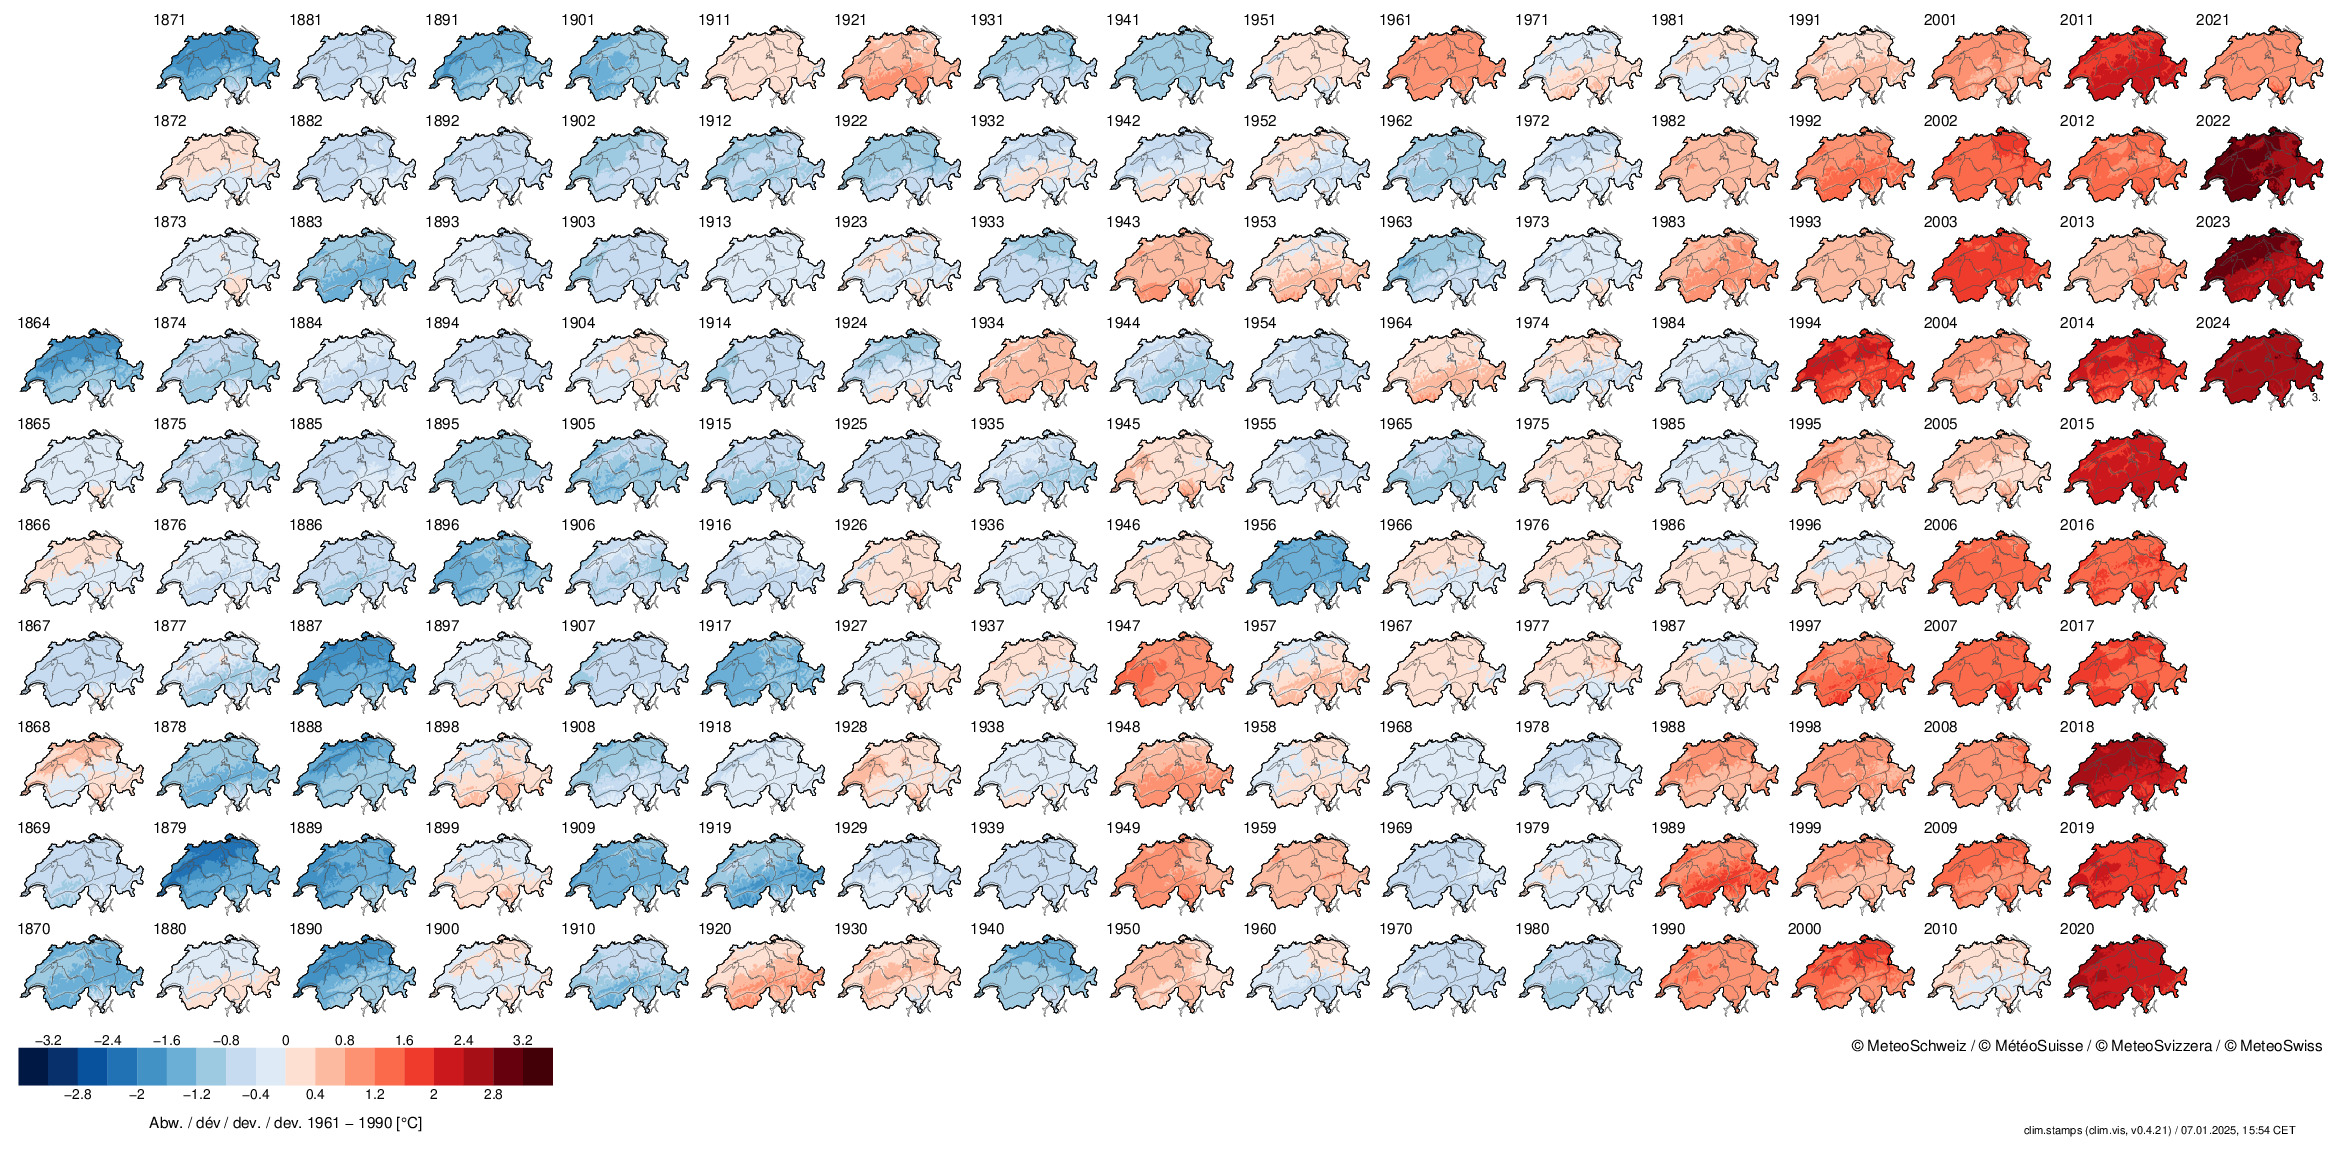
\includegraphics[keepaspectratio]{3_ecological-sustainability/images/Fig3_9__KlimaCH.jpg}}

}

\caption{\label{fig-worlds}Der Klimawandel in der Schweiz von 1864 bis
2024. Quelle:
\url{https://www.nccs.admin.ch/nccs/en/home/climate-change-and-impacts/climate-basics/what-is-climate-.html}.}

\end{figure}%

Das \textbf{Pariser Klimaabkommen}, das im Dezember 2015 verabschiedet
wurde, war der erste internationale Vertrag, in dem Industrie- und
Schwellenländer gemeinsam zusagten, die Treibhausgasemissionen zu
reduzieren. Sein Kernziel ist es, den globalen Temperaturanstieg auf
maximal 2°C zu begrenzen, mit Bemühungen um eine Beschränkung auf 1,5°C
gegenüber dem vorindustriellen Niveau. Im Jahr 2018 veröffentlichte der
Zwischenstaatliche Ausschuss für Klimaänderungen (IPCC) einen
Sonderbericht mit einigen bemerkenswerten Erkenntnissen: vor allem, dass
wir nur noch wenige Jahre -- bis 2030 -- Zeit haben, um zu verhindern,
dass die 2°C-Grenze überschritten wird. Die nächste wichtige
Entscheidung im Rahmen der internationalen Klimabemühungen im Anschluss
an das Pariser Abkommen war die Klimakonferenz COP 27 im Jahr 2022. Auf
der COP 27 einigten sich die Unterzeichnenden auf die Einrichtung des
Fonds für Verluste und Schäden (Loss and Damage Fund) -- das Ergebnis
jahrzehntelanger Diskussionen --, der Entwicklungsländern nach extremen
Wetterereignissen finanzielle Unterstützung ermöglichen soll.

\begin{tcolorbox}[enhanced jigsaw, arc=.35mm, bottomrule=.15mm, bottomtitle=1mm, breakable, colback=white, colbacktitle=quarto-callout-note-color!10!white, colframe=quarto-callout-note-color-frame, coltitle=black, left=2mm, leftrule=.75mm, opacityback=0, opacitybacktitle=0.6, rightrule=.15mm, title={Der Zwischenstaatliche Ausschuss für Klimaänderungen (IPCC)}, titlerule=0mm, toprule=.15mm, toptitle=1mm]

Der \textbf{Zwischenstaatliche Ausschuss für Klimaänderungen (IPCC)},
1988 von den Vereinten Nationen und der Weltorganisation für
Meteorologie gegründet, fasst die wissenschaftliche Forschung zum
Klimawandel für politische Entscheidungsträger*innen weltweit zusammen.
Seine regelmässig erscheinenden IPCC-Berichte liefern eine umfassende
Bewertung des aktuellen Wissensstands zum Klimawandel, einschliesslich
der physikalischen Grundlagen, Auswirkungen, Risiken und
Anpassungsstrategien. Diese Berichte basieren auf Tausenden von Studien
und gelten als die massgeblichste Informationsquelle zum Klimawandel.
Die IPCC-Berichte dienen als Grundlage für internationale Verhandlungen
und nationale Klimapolitiken, einschliesslich des Pariser Abkommens von
2015.

\end{tcolorbox}

\begin{figure}[H]

\centering{

\pandocbounded{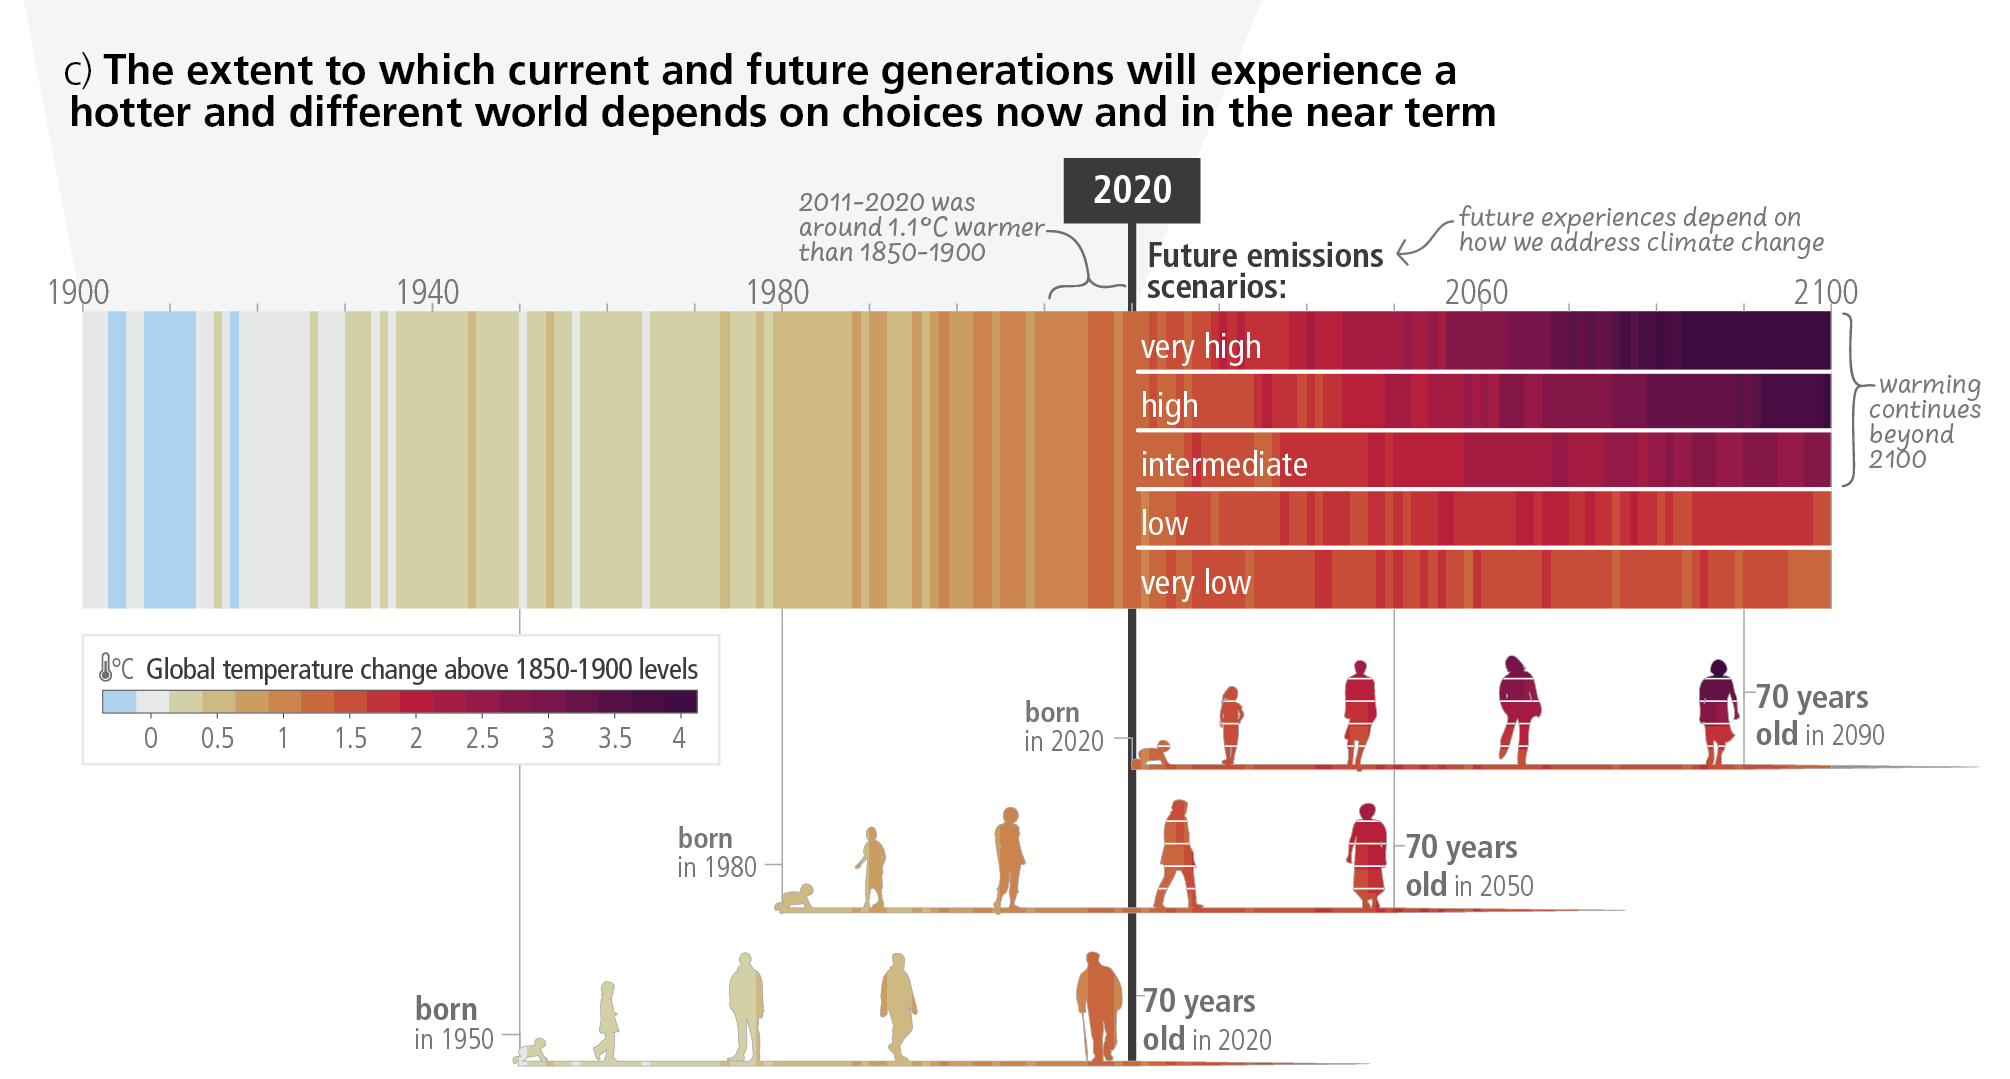
\includegraphics[keepaspectratio]{3_ecological-sustainability/images/Fig3_10__IPCCas6Fig2.png}}

}

\caption{\label{fig-hotter-and-different-world}Auszug aus dem
AR6-Synthese-Bericht, Abbildung SPM.1 (c): Beobachtete (1900--2020) und
projizierte (2021--2100) Veränderungen der globalen
Oberflächentemperatur (relativ zu 1850--1900), die mit Veränderungen der
Klimabedingungen und Auswirkungen verknüpft sind, zeigen, wie sich das
Klima bereits verändert hat und sich über die Lebensspanne von drei
repräsentativen Generationen (geboren 1950, 1980 und 2020) verändern
wird. Quelle: IPCC (2023).}

\end{figure}%

Doch was ist nötig, um zu verhindern, dass die Temperatur um mehr als
1,5 Grad ansteigt? Eine ganze Menge. Die anthropogenen
CO\textsubscript{2}-Emissionen müssen zwischen 2010 und 2030 um 45\%
sinken, und die Netto-CO\textsubscript{2}-Emissionen müssen bis 2050 auf
null reduziert werden. Während wir für marginale Aktivitäten wie
Autokäufe oder Gebäudesanierungen grünere Technologien einsetzen,
riskieren wir dennoch, die ernsthafte Bedrohung durch den bereits in der
Atmosphäre vorhandenen Kohlenstoff zu vernachlässigen. Es ist wichtig,
zwischen laufenden Emissionen (Fluss) und dem angesammelten
atmosphärischen Kohlenstoff (Bestand) zu unterscheiden. Der Fluss spielt
für den Planeten eine untergeordnete Rolle -- es ist der Bestand, der
die globale Erwärmung antreibt. Der Klimawandel ist daher in erster
Linie ein Bestandsproblem und kein Flussproblem. Dies ist ein
anspruchsvolles Konzept, nicht nur für Laien. Tatsächlich stellten
Sterman und Sweeney (2007) fest, dass die meisten Erwachsenen
Schwierigkeiten hatten, den Bestandsaspekt des Klimawandels zu erfassen.

\begin{figure}[H]

\centering{

\pandocbounded{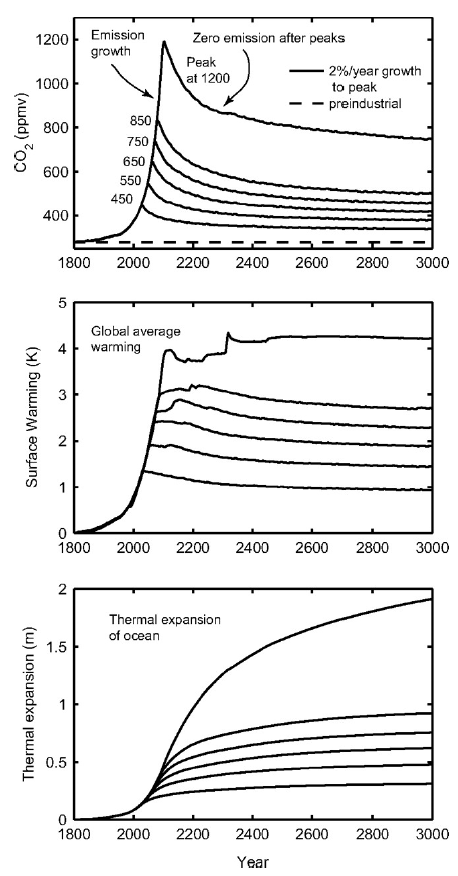
\includegraphics[keepaspectratio]{3_ecological-sustainability/images/Solomon.png}}

}

\caption{\label{fig-change-to-various-components}Kohlendioxid und
globale Veränderungen des Klimasystems (im Vergleich zu den
vorindustriellen Bedingungen im Jahr 1765). Quelle: Solomon u.~a.
(2009).}

\end{figure}%

Ein wirksames mentales Modell ist die Badewannen-Analogie: Wenn der
Zufluss durch den Hahn (d.~h. unsere Emissionen, der Fluss) den Abfluss
(Kohlenstoffaufnahme durch Regenwälder, Ozeane usw.) übersteigt, steigt
der Wasserspiegel (der atmosphärische Kohlenstoffbestand). Die letzten
fünf Jahre und zwanzig der letzten zweiundzwanzig Jahre waren die
wärmsten seit Beginn der Aufzeichnungen. Dieser Erwärmungstrend ist eine
direkte Folge des steigenden Wasserstands in dieser „Badewanne''.

\textbf{Auswirkungen}: Es wird erwartet, dass der Klimawandel eine Reihe
direkter und indirekter Folgen hat, von denen einige bereits eintreten.
Dazu gehören der Meeresspiegelanstieg, schwindende Gletscher,
Bedrohungen der Wasser- und Ernährungssicherheit, eine Zunahme extremer
Wetterereignisse, negative gesundheitliche Auswirkungen im Zusammenhang
mit Temperatur, Hitzewellen, Dürren und Starkniederschlägen, Waldbrände
sowie eine Zunahme geomorphologischer Aktivitäten und damit verbundener
Naturgefahren infolge des Permafrosttauens.

\subsection{Landnutzungsveränderungen}\label{landnutzungsveruxe4nderungen}

Landnutzungsveränderungen -- wie Entwaldung für die Landwirtschaft oder
städtische Expansion -- haben einen erheblichen Einfluss auf die
\textbf{ökologische Dimension der Nachhaltigkeit}. Sie bedrohen die
Biodiversität und stören die Ökosystemfunktionen. Sie können auch
Treibhausgasemissionen erhöhen, Wasserkreisläufe verändern oder
wertvolles Agrarland erschöpfen. Dies kann zu einer Verringerung der
Ökosystemdienstleistungen führen (vgl. \emph{Kapitel 3.2 zu Ökosystemen,
Ökosystemmanagement und Ökosystemdienstleistungen}), was letztlich das
menschliche Wohlergehen einschränkt. Landnutzungsveränderungen sind eine
der neun \textbf{planetaren Grenzen}, die laut Richardson u.~a. (2023)
bereits überschritten wurde.

Zum Verständnis von Landnutzungsveränderungen sind einige
Schlüsseldefinitionen erforderlich:

\begin{itemize}
\item
  \textbf{Landbedeckung} bezeichnet die Eigenschaften der Landoberfläche
  und ihrer unmittelbaren Unterfläche, einschliesslich Biota,
  Topographie und menschlicher Bauwerke (Lambin u.~a. 2000, p.~322).
\item
  \textbf{Landnutzung} ist die Art und Weise, wie Menschen die
  Landbedeckung nutzen (Lambin u.~a. 2000, p.~322).
\item
  \textbf{Landnutzungsveränderung} bezeichnet den Wechsel von einer
  Landnutzungsart zu einer anderen (Lambin u.~a. 2000, p.~322).
\item
  \textbf{Landdegradation} bedeutet „Verringerung oder Verlust der
  biologischen oder wirtschaftlichen Produktivität und Komplexität von
  Regenfeldbau, Bewässerungsfeldbau oder Weide-, Wald- und Waldland in
  ariden, semi-ariden und trockenen subhumiden Gebieten infolge von
  Landnutzungen'' (UN 1994, p.~4).
\item
  \textbf{Landsysteme} „repräsentieren die terrestrische Komponente des
  Erdsystems und umfassen alle Prozesse und Aktivitäten im Zusammenhang
  mit der menschlichen Landnutzung, einschliesslich sozioökonomischer,
  technologischer und organisatorischer Investitionen und Vereinbarungen
  sowie der Vorteile, die aus dem Land gewonnen werden, und der
  unbeabsichtigten sozialen und ökologischen Folgen gesellschaftlicher
  Aktivitäten'' (Verburg u.~a. 2013, p.~433).
\item
  Land kann auch als ein \textbf{sozial-ökologisches System} (Chapin
  u.~a. 2006) verstanden werden, in dem die sozialen und ökologischen
  Teilsysteme miteinander interagieren und voneinander abhängen. Dieses
  System ist durch gegenseitige Rückkopplung gekennzeichnet, wobei der
  Mensch als integraler Bestandteil der Natur betrachtet wird (Verburg
  u.~a. 2015).
\end{itemize}

Verschiedene \textbf{Treiber}, d.~h. Gründe oder Ursachen, sind für das
Auftreten von Landnutzungsveränderungen verantwortlich. Diese Faktoren
variieren je nach Art der Landnutzung. Die Haupttreiber der globalen
Entwaldung -- eine Form der Landnutzungsveränderung -- sind
beispielsweise die kommerzielle Landwirtschaft, der Wanderfeldbau, die
kommerzielle Forstwirtschaft, die Urbanisierung und Waldbrände (Curtis
u.~a. 2018). Die Entwaldung hat bereits zu einem alarmierenden Rückgang
der Biodiversität (vgl. \emph{Kapitel 3.4 zu Biodiversitätsverlust}) und
zur Unterbrechung von Kohlenstoffkreisläufen geführt (vgl. \emph{Kapitel
3.2 zu Ökosystemen, Ökosystemmanagement und Ökosystemdienstleistungen}).
So ist der Sektor Landwirtschaft, Forstwirtschaft und andere Landnutzung
(AFOLU) ein wesentlicher Verursacher \textbf{globaler anthropogener
Treibhausgasemissionen} und macht etwa 13\% der CO\textsubscript{2}-,
44\% der CH\textsubscript{4}- und 81\% der
N\textsubscript{2}O-Emissionen aus (IPCC 2019). Diese Wechselwirkungen
zwischen Klimawandel und Landnutzung bzw. Landnutzungsveränderungen
zeigen, dass Landsysteme und Klimasysteme systemisch und nicht isoliert
betrachtet werden sollten (Richardson u.~a. 2023).
Abbildung~\ref{fig-land-climate-interaction} zeigt eine schematische
Darstellung dieser Wechselwirkungen zwischen Land und Treibhausgasen.

\begin{figure}[H]

\centering{

\pandocbounded{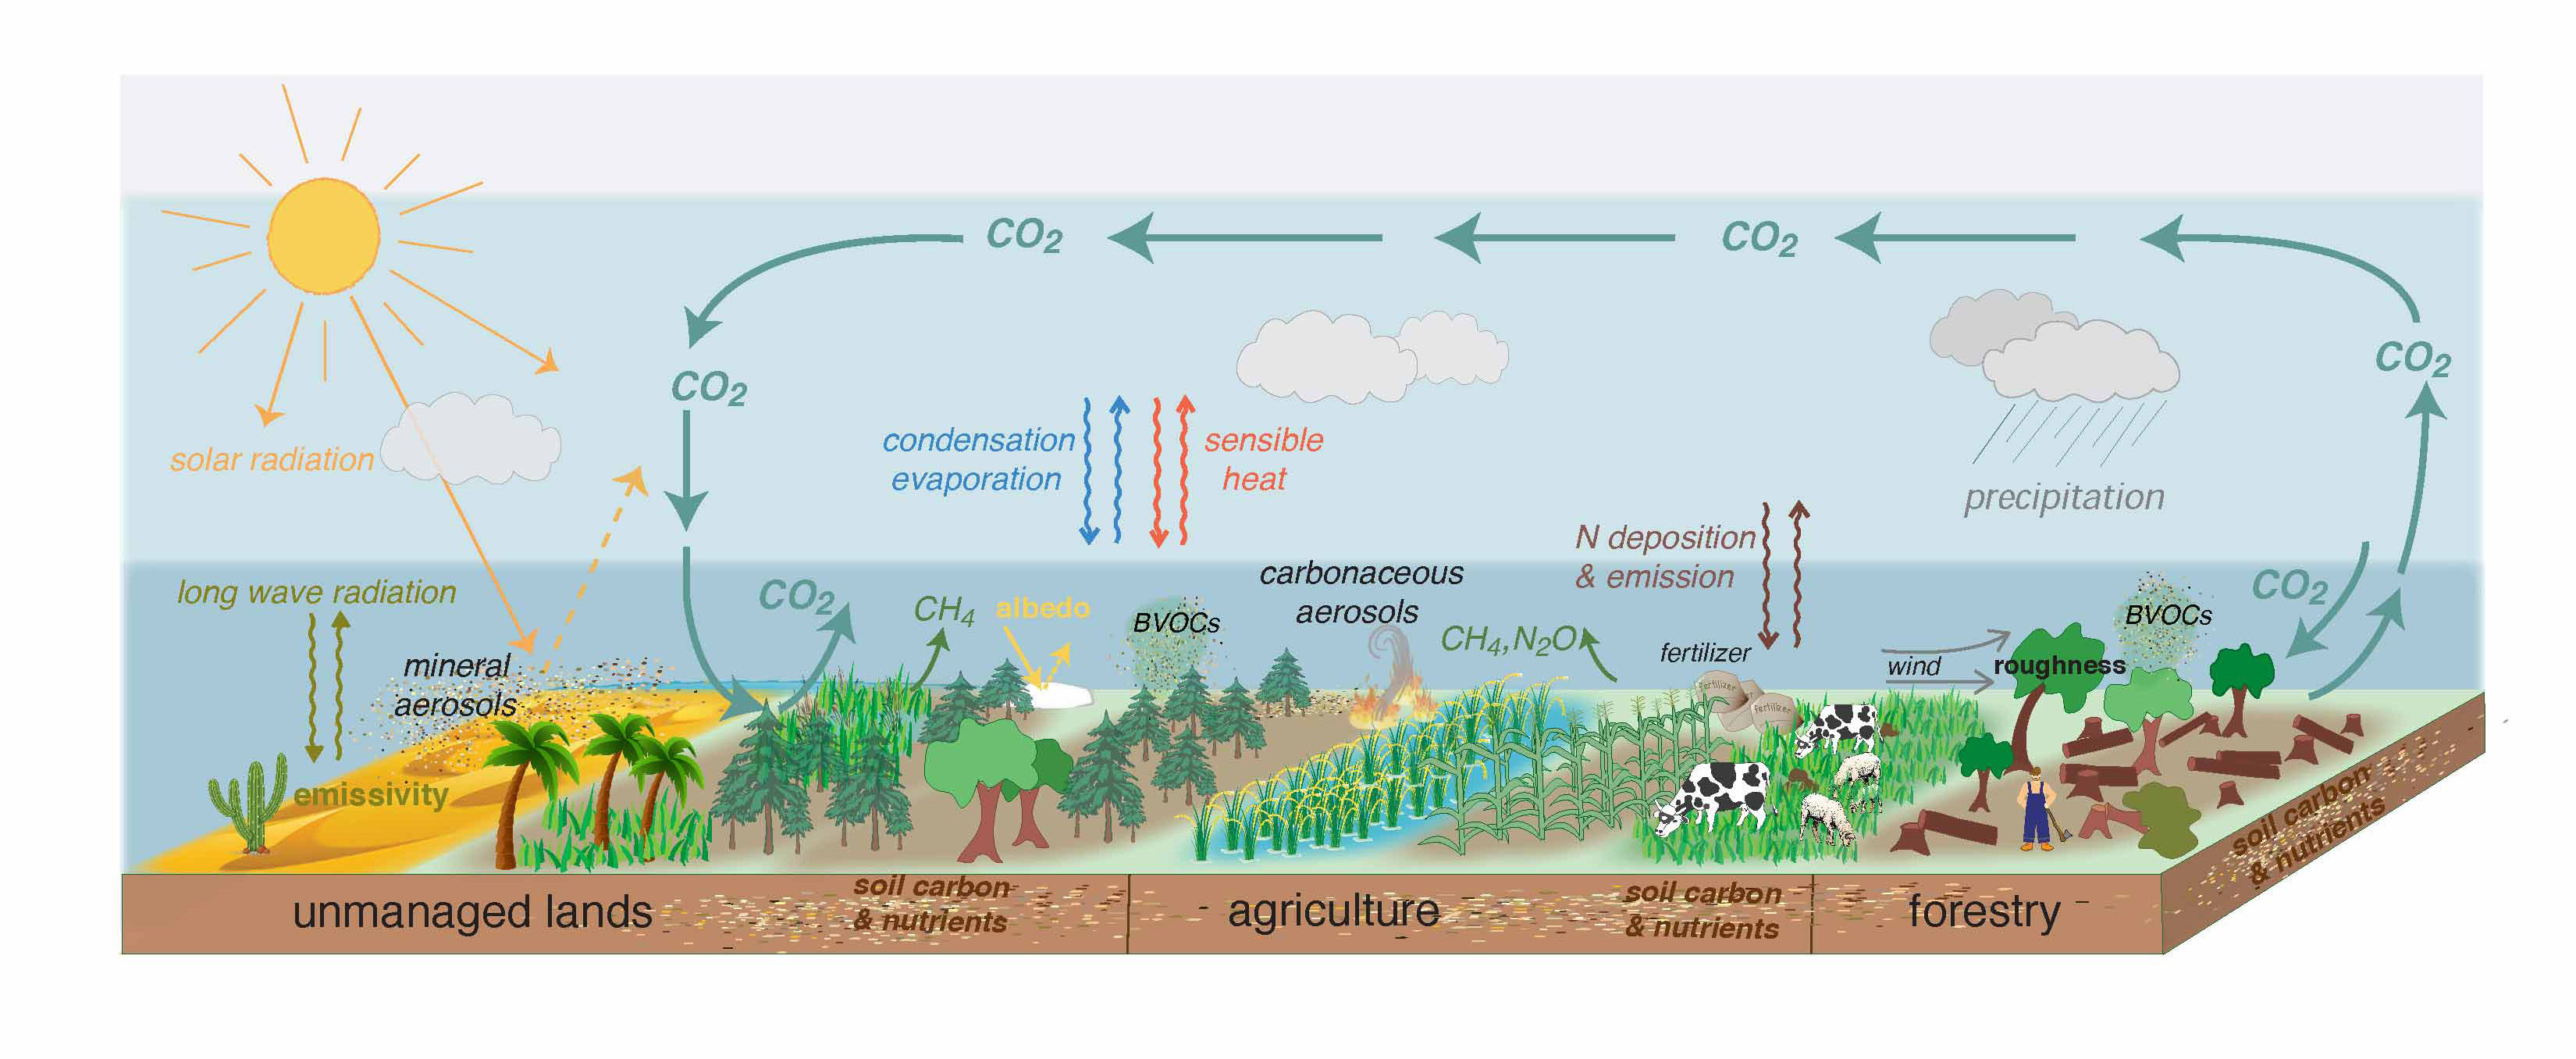
\includegraphics[keepaspectratio]{3_ecological-sustainability/images/Fig3_11__LandClimateInteraction.png}}

}

\caption{\label{fig-land-climate-interaction}Struktur und Funktionsweise
bewirtschafteter und unbewirtschafteter Ökosysteme, die das lokale,
regionale und globale Klima beeinflussen. Quelle: IPCC (2019).}

\end{figure}%

Über ihre Auswirkungen auf klimarelevante Treibhausgasflüsse hinaus
stören Landnutzung und Landnutzungsveränderungen auch andere
\textbf{biogeochemische Materialkreisläufe}, wie Nitrat-, Phosphor- oder
Schwefelkreisläufe, und verknüpfen sie mit einer weiteren bereits
überschrittenen planetaren Grenze -- derjenigen der biogeochemischen
Kreisläufe (Richardson u.~a. 2023). Ein klassisches Beispiel hierfür ist
die \textbf{Eutrophierung}, ein Prozess, der auftritt, wenn
landwirtschaftliche Düngemittel wie Phosphor in nährstoffarme Gewässer
gelangen und zu übermässigem Algenwachstum, sogenannten Algenblüten,
führen. Wenn diese Blüten verrotten, verringern sie den
Sauerstoffgehalt, was aquatisches Leben letztlich einschränkt oder gar
verhindert (Galloway u.~a. 2008; Smith u.~a. 2006).

\begin{tcolorbox}[enhanced jigsaw, arc=.35mm, bottomrule=.15mm, bottomtitle=1mm, breakable, colback=white, colbacktitle=quarto-callout-tip-color!10!white, colframe=quarto-callout-tip-color-frame, coltitle=black, left=2mm, leftrule=.75mm, opacityback=0, opacitybacktitle=0.6, rightrule=.15mm, title={Landnutzungsveränderungen in den Tropen: das Beispiel Madagaskar}, titlerule=0mm, toprule=.15mm, toptitle=1mm]

In den Tropen sind die am besten an lokale Bedingungen angepassten
Anbauformen (d.~h. ohne Dünger oder andere Betriebsmittel)
Agroforstwirtschaft und Brandrodung. \textbf{Agroforstwirtschaft} ist
ein dauerhaftes Landnutzungssystem, in dem einjährige Feldfrüchte
zusammen mit Bäumen angebaut werden oder mehrjährige Kulturen (z. B.
Maniok, Vanille, Bananen und Lychees) gemeinsam gepflanzt werden.
\textbf{Brandrodung}, auch bekannt als \textbf{Wanderfeldbau},
bezeichnet dagegen ein Landnutzungssystem, bei dem jedes Jahr eine
andere Fläche gerodet und eine Ernte wie Mais angebaut wird, während die
zuvor bebauten Felder brachliegen, um den Aufbau von Nährstoffen zu
ermöglichen.

Wie oben erwähnt, ist die Brandrodung, wie sie in Madagaskar praktiziert
wird, eine der Hauptursachen der globalen Entwaldung. Daher bekämpfen
Regierungen und NGOs die Brandrodung seit der Kolonialzeit. Eine
Herausforderung bei der Brandrodung ist, dass Bäuer*innen, wenn die
Brachzeiten aufgrund von Landmangel zu kurz werden, in bisher ungenutzte
Waldgebiete ausweichen und diese roden, um den Brandrodungszyklus
aufrechtzuerhalten. Diese Entwaldung erzeugt erhebliche Biomasse, die
verbrannt werden muss. In Madagaskar beispielsweise wurden innerhalb
eines Monats von Mitte September bis Mitte Oktober 2023 mehr als 6.000
Brandstellen registriert.

Deshalb wird der lokalen Bevölkerung die Verantwortung für die
Entwaldung in Madagaskar zugeschrieben. Doch Brandrodung ist eine
notwendige Überlebensstrategie für die Einheimischen, die kaum
Alternativen haben und auf sie angewiesen sind, um Land für künftige
Generationen zu sichern. Dieser Zielkonflikt ist spezifisch ein
\textbf{Landnutzungskonflikt}.

\end{tcolorbox}

\begin{tcolorbox}[enhanced jigsaw, arc=.35mm, bottomrule=.15mm, bottomtitle=1mm, breakable, colback=white, colbacktitle=quarto-callout-tip-color!10!white, colframe=quarto-callout-tip-color-frame, coltitle=black, left=2mm, leftrule=.75mm, opacityback=0, opacitybacktitle=0.6, rightrule=.15mm, title={Landnutzungskonflikte in der Schweiz: der Solar Express}, titlerule=0mm, toprule=.15mm, toptitle=1mm]

Ein weiteres Beispiel für einen Landnutzungskonflikt zeigt sich in der
Schweiz, bei einem Interessenkonflikt zwischen einem dezentralen
erneuerbaren Energieprojekt und Landschaftsdienstleistungen (vgl.
Kienast u.~a. 2017). Im Jahr 2022 lancierte die Schweizer Regierung eine
„Solaroffensive'' in Form eines Projekts namens „Solar Express''. Ziel
war es, alpine Photovoltaikanlagen durch hohe Subventionen zu fördern,
die bis zu 60\% der Investitionskosten abdecken sollten. Im Sommer 2024
fand in Sedrun, im östlichsten Kanton Graubünden, der Spatenstich für
die erste Grossanlage mit einer Fläche von 300.000 m\textsuperscript{2}
statt. Solche Grossanlagen kollidieren jedoch mit anderen Landnutzungen
und beeinträchtigen insbesondere Agrarflächen, Naturschutzgebiete und
Tourismusregionen. Solaranlagen verändern die Landschaft und könnten
Flora und Fauna beeinflussen, was bei Bäuer*innen und
Naturschutzorganisationen Befürchtungen über den Verlust von wertvollem
Ackerland und Biodiversitätsflächen weckt. Gleichzeitig fordern
Befürworter*innen erneuerbarer Energien die rasche Umsetzung dieser
Projekte, um die Abhängigkeit der Schweiz von fossilen Brennstoffen zu
reduzieren und das Klima zu schützen. Dies verdeutlicht die Spannung
zwischen dem Bedarf an erneuerbaren Energien einerseits und dem Wunsch,
Landschaft und Umwelt zu erhalten, andererseits.

\end{tcolorbox}

Die Entwaldung in tropischen Regionen ist eine Form der
Landnutzungsveränderung, die nicht nur von lokalen Bedürfnissen, sondern
auch von internationalen Entscheidungen und Nachfragen beeinflusst wird
(Curtis u.~a. 2018). Dies legt nahe, dass die Verhinderung von
Entwaldung sowohl auf lokaler als auch auf internationaler Ebene
angegangen werden muss (DeFries u.~a. 2010). Doch nicht nur die
Entwaldung, sondern Landnutzungsveränderungen allgemein werden von
entfernten Faktoren beeinflusst (Meyfroidt u.~a. 2013). In der
Wissenschaft werden solche Phänomene und Prozesse als
\textbf{Telekopplung} bezeichnet ({Liu u.~a.} 2013). Telekopplung
beschreibt die sozioökonomischen und ökologischen Wechselwirkungen
zwischen weit entfernten menschlichen und natürlichen Systemen und
analysiert, wie Handlungen an einem Ort (dem Sendesystem) einen anderen
Ort (das Empfangssystem) beeinflussen können. So verlangen neue
EU-Verordnungen, dass Produkte, die ab Ende 2024 in den EU-Markt
eingeführt werden, entwaldungsfrei sein müssen
(\href{https://environment.ec.europa.eu/topics/forests/deforestation/regulation-deforestation-free-products_en}{Verordnung
über entwaldungsfreie Produkte -- Europäische Kommission (europa.eu)}).
Diese Verordnungen werden voraussichtlich erhebliche ökologische (und
soziale) Auswirkungen in den Anbauländern haben (Coenen u.~a. 2023).

\begin{tcolorbox}[enhanced jigsaw, arc=.35mm, bottomrule=.15mm, bottomtitle=1mm, breakable, colback=white, colbacktitle=quarto-callout-note-color!10!white, colframe=quarto-callout-note-color-frame, coltitle=black, left=2mm, leftrule=.75mm, opacityback=0, opacitybacktitle=0.6, rightrule=.15mm, title={Landrechte und Landbesitz}, titlerule=0mm, toprule=.15mm, toptitle=1mm]

Landnutzung und Landnutzungsveränderungen sind eng mit Fragen der
\textbf{Landrechte} und des \textbf{Landbesitzes} verknüpft, da diese
Faktoren massgeblich bestimmen, wer zur Nutzung von Land berechtigt ist
und wie es genutzt wird. Sicherer Landbesitz und klar definierte
Landrechte sind entscheidend für nachhaltige Landnutzungspraktiken, da
sie langfristige Investitionen in das Landmanagement fördern und den
Schutz von Ressourcen begünstigen. Unsichere oder unklare Landrechte
können hingegen zu Landnutzungsveränderungen führen, die die Umwelt
schädigen, wie unkontrollierte Entwaldung. Diese Fragen werden im
Zusammenhang mit \textbf{Landraub} besonders brisant, bei dem grosse
Landflächen von ausländischen (oder auch inländischen) Investor*innen
erworben werden, oft ohne angemessene Konsultation oder Entschädigung
der lokalen Bevölkerung. Landraub kann zu Konflikten führen, die
bestehende Landrechte untergraben und die Landnutzung auf eine Weise
verändern, welche die ökologische und soziale Nachhaltigkeit gefährdet.

\end{tcolorbox}

Dieses Kapitel hat gezeigt, dass Land, Landnutzung und
Landnutzungsveränderungen ein vielschichtiges Thema sind. Um die
Bedeutung dieses Themas zu unterstreichen, haben {Meyfroidt u.~a.}
(2022) zehn Fakten über Landsysteme für die Nachhaltigkeit
zusammengefasst (Abbildung~\ref{fig-ten-facts}, links), die auf
empirischer Forschung basieren. Diese Fakten führen wiederum zu zehn
damit verbundenen Herausforderungen ({Meyfroidt u.~a.} 2022). Fakt 2
etwa („\emph{Land als komplexe Systeme}'') führt zu der Herausforderung,
dass die Folgen von Eingriffen in Landsysteme schwer vorherzusagen und
zu verstehen sind, was die Entwicklung wirksamer Massnahmen oder
Politiken zur Landnutzung erschwert. Einige der in diesem Kapitel
diskutierten Themen stimmen mit diesen Fakten überein, beispielsweise
Telekopplung und Fakt 5, „\emph{Entfernte Verbindungen}''.

\begin{figure}[H]

\centering{

\pandocbounded{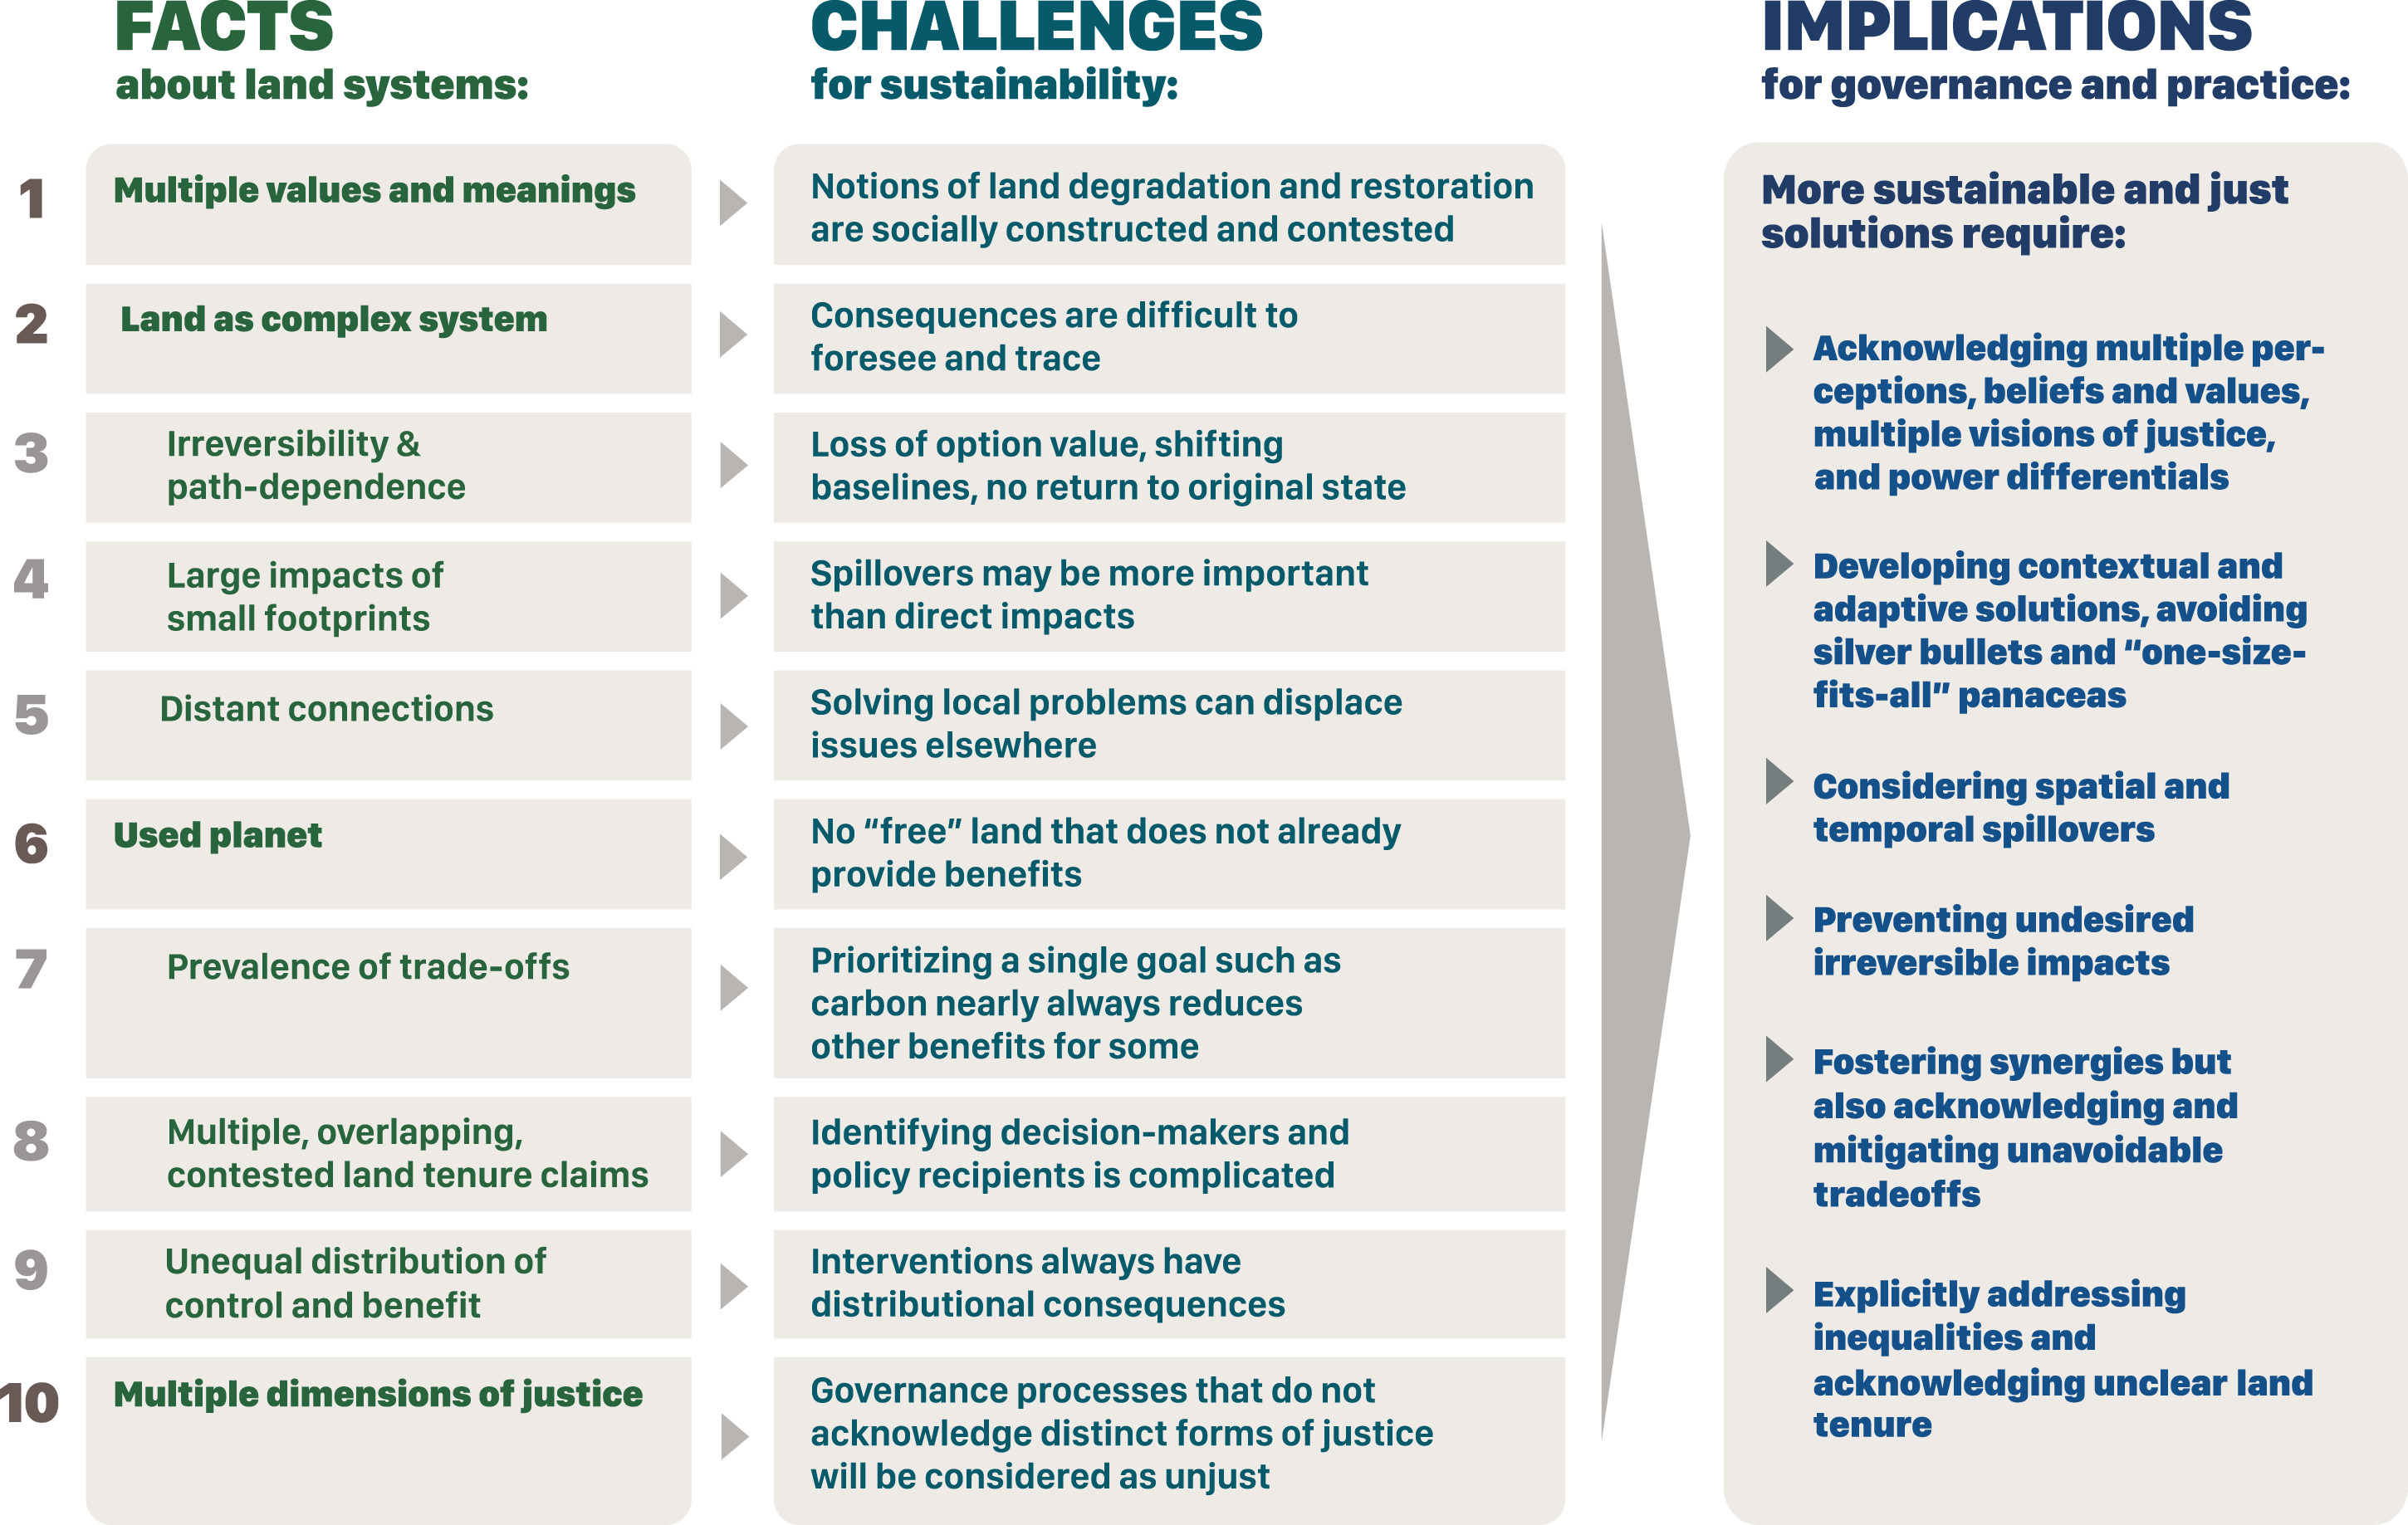
\includegraphics[keepaspectratio]{3_ecological-sustainability/images/Fig3_12_FactsChallenges.jpg}}

}

\caption{\label{fig-ten-facts}Zehn empirische Realitäten (Fakten) über
Landsysteme mit starker allgemeiner Unterstützung. Herausforderungen
fassen die Probleme zusammen, die sich aus jedem Fakt ergeben, wenn man
versucht, Landsysteme für die Nachhaltigkeit zu managen und zu regieren.
Implikationen fassen zusammen, wie die Governance von Landsystemen für
die Nachhaltigkeit verbessert werden könnte, indem diese Fakten und
Herausforderungen anerkannt werden. Die 10 Fakten sind durch vier
übergeordnete Fakten (1, 2, 6 und 10) und mehrere untergeordnete Fakten
strukturiert, die von diesen abgeleitet werden (3, 4 und 5 von 2; 7, 8
und 9 von 6), aber alle spezifische Realitäten ausdrücken, die
spezifische Herausforderungen implizieren. Quelle: {Meyfroidt u.~a.}
(2022), lizenziert unter CC BY 4.0}

\end{figure}%

\begin{tcolorbox}[enhanced jigsaw, arc=.35mm, bottomrule=.15mm, bottomtitle=1mm, breakable, colback=white, colbacktitle=quarto-callout-tip-color!10!white, colframe=quarto-callout-tip-color-frame, coltitle=black, left=2mm, leftrule=.75mm, opacityback=0, opacitybacktitle=0.6, rightrule=.15mm, title={Beispiel: Landinvestitionen in Laos}, titlerule=0mm, toprule=.15mm, toptitle=1mm]

Ein weiteres Beispiel für Landnutzungsveränderungen und ihre
weitreichenden Auswirkungen sind kommerzielle Landinvestitionen in Laos.
Die Demokratische Volksrepublik Laos ist ein bergiges Binnenland mit
einer hohen Armutsquote und einigen wenigen kleinen städtischen Zentren.
Laos liegt zwischen China, Vietnam, Thailand, Kambodscha und Myanmar und
öffnete sich in den 1990er Jahren aus seiner kommunistischen Isolation.
Das Land ist reich an natürlichen Ressourcen wie Land, Wäldern und
Mineralien. Um das nationale Wirtschaftswachstum zu fördern, verfolgt
die Regierung von Laos eine Strategie der „\textbf{Umwandlung von Land
in Kapital}'', d.~h. der Umwandlung von „ungenutztem'' Land in
produktives Land, in der Hoffnung, durch Spillover-Effekte eine
ländliche Entwicklung zu erzielen. Diese Strategie wird hauptsächlich
durch kommerzielle Landinvestitionen umgesetzt, bei denen die Regierung
inländischen und ausländischen Investor*innen Landkonzessionen erteilt.

Doch inwiefern trägt diese Politik tatsächlich zur nachhaltigen
Entwicklung bei? Um dies herauszufinden, arbeiteten
Wissenschaftler*innen des Centre for Development and Environment (CDE)
mit der Regierung von Laos zusammen, um Landkonzessionen zu erfassen und
die Qualität der Investitionen zu untersuchen. Es wurde ein nationales
digitales Informationssystem entwickelt, das Laos ermöglicht, seine
Landkonzessionen effektiv zu verwalten. Das System zeigte auch, dass
nicht alle Investor*innen ihre Versprechen einhalten, was die
Nachhaltigkeit dieser Landnutzungsstrategie in Frage stellt.

Die Landnutzungsveränderungen hin zu Bananenplantagen, anderen
Baumplantagen wie Kautschukplantagen, Minen und Wasserkraftprojekten
führten unter anderem zu einem Verlust an Waldflächen -- etwa ein
Drittel aller Konzessionen wurde in nationalen Waldgebieten erteilt.
Dies führte auch zu einem Verlust wichtiger Ökosystemdienstleistungen
und einem Rückgang der Biodiversität. Über die ökologischen Auswirkungen
auf die lokale Umwelt hinaus hatten die Landinvestitionen auch
sozioökonomische Konsequenzen. Obwohl für einige das finanzielle
Einkommen gestiegen ist, wirkten sich die Landinvestitionen in vielen
Gebieten negativ auf das Wohlbefinden der lokalen Bevölkerung aus und
beeinträchtigten die Ernährungssicherheit sowie den Zugang zu Land und
natürlichen Ressourcen, die für subsistenzorientierte Lebensweisen
unerlässlich sind (Nanhthavong u.~a. 2021; Hett u.~a. 2020).

\url{https://youtu.be/J6QpmuWYbfE?si=mkIRErt6Khp6Vpca}

\end{tcolorbox}

\section{Biodiversitätsverlust}\label{biodiversituxe4tsverlust}

Biodiversität ist definiert als die Vielfalt des Lebens in all seinen
Formen, von Genen über Arten bis hin zu Ökosystemen (UN 1992a). Sie ist
eine wesentliche Grundlage für das Wohlergehen der Menschheit und damit
ein wesentlicher Bestandteil der \textbf{ökologischen Nachhaltigkeit},
die die Basis für zahlreiche Ökosystemdienstleistungen (Haines-Young und
Potschin-Young 2010) oder Naturbeiträge für Menschen (Antunes u.~a.
2024) bildet. Biodiversität ist auch eng mit mehreren \textbf{planetaren
Grenzen} verknüpft, insbesondere mit Landnutzungsveränderungen und der
Integrität der Biosphäre ({Steffen u.~a.} 2015). Es ist klar, dass ein
unkontrollierter Biodiversitätsverlust Kipppunkte in Ökosystemen
auslösen, das Gleichgewicht der Erde stören und die Fähigkeit unseres
Planeten, menschliches Leben zu erhalten, schwer beeinträchtigen könnte.
Der Schutz und die Wiederherstellung der Biodiversität gelten daher als
Schlüssel zu einer nachhaltigen Zukunft.

Dennoch befindet sich die \textbf{Biodiversität} derzeit in einem
alarmierenden Zustand (vgl. Infokasten unten). Weltweit nimmt die
Artenvielfalt seit mehreren Jahrzehnten ab ({Butchart u.~a.} 2010; Díaz
und Malhi 2022), ein Abwärtstrend, der laut Prognosen anhalten wird
(Díaz und Malhi 2022). Infolgedessen wird bereits ein sechstes
Massenaussterben diskutiert (Ceballos u.~a. 2020). Um dieser Entwicklung
entgegenzuwirken, wurde das \textbf{Übereinkommen über die biologische
Vielfalt (CBD)} auf dem Rio-Erdgipfel 1992 ratifiziert (UN 1992a), unter
Schweizer Beteiligung. Dieses rechtlich bindende Abkommen bedeutet, dass
neue Bestimmungen, die an nachfolgenden Konferenzen beschlossen werden,
rechtlich umgesetzt werden müssen, wenn die Schweiz Delegierte schickt.

\begin{tcolorbox}[enhanced jigsaw, arc=.35mm, bottomrule=.15mm, bottomtitle=1mm, breakable, colback=white, colbacktitle=quarto-callout-note-color!10!white, colframe=quarto-callout-note-color-frame, coltitle=black, left=2mm, leftrule=.75mm, opacityback=0, opacitybacktitle=0.6, rightrule=.15mm, title={Monitoring}, titlerule=0mm, toprule=.15mm, toptitle=1mm]

Das Biodiversitätsmonitoring ist ein wichtiges Instrument zur Verfolgung
von Veränderungen in der Biodiversität. Die Rote Liste gefährdeter Tier-
und Pflanzenarten der Internationalen Union zur Bewahrung der Natur
(IUCN), die seit 1964 geführt wird, spielt dabei eine besonders wichtige
Rolle. Sie kategorisiert den Status einer Art in eine von neun
Kategorien, von „nicht gefährdet'' bis „ausgestorben''. Abbildung
Abbildung~\ref{fig-IUCN-red-list} zeigt beispielsweise den Prozentsatz
der Arten in jeder Kategorie auf globaler Ebene. Dieselben Kategorien
werden auch in der Schweiz verwendet. Solche Datenbanken helfen unter
anderem, die Politikgestaltung und Naturschutzplanung zu verbessern und
eine angemessenere Zuweisung von (finanziellen) Ressourcen in Forschung
und Gesellschaft zu ermöglichen. Trotz des umfangreichen und etablierten
Artenmonitorings gehen vorsichtige Studien davon aus, dass nur zwischen
1,5\% und 18\% der terrestrischen Wirbeltierspezies unseres Planeten
identifiziert und beschrieben wurden (vgl. Moura und Jetz 2021).

\begin{figure}[H]

\centering{

\pandocbounded{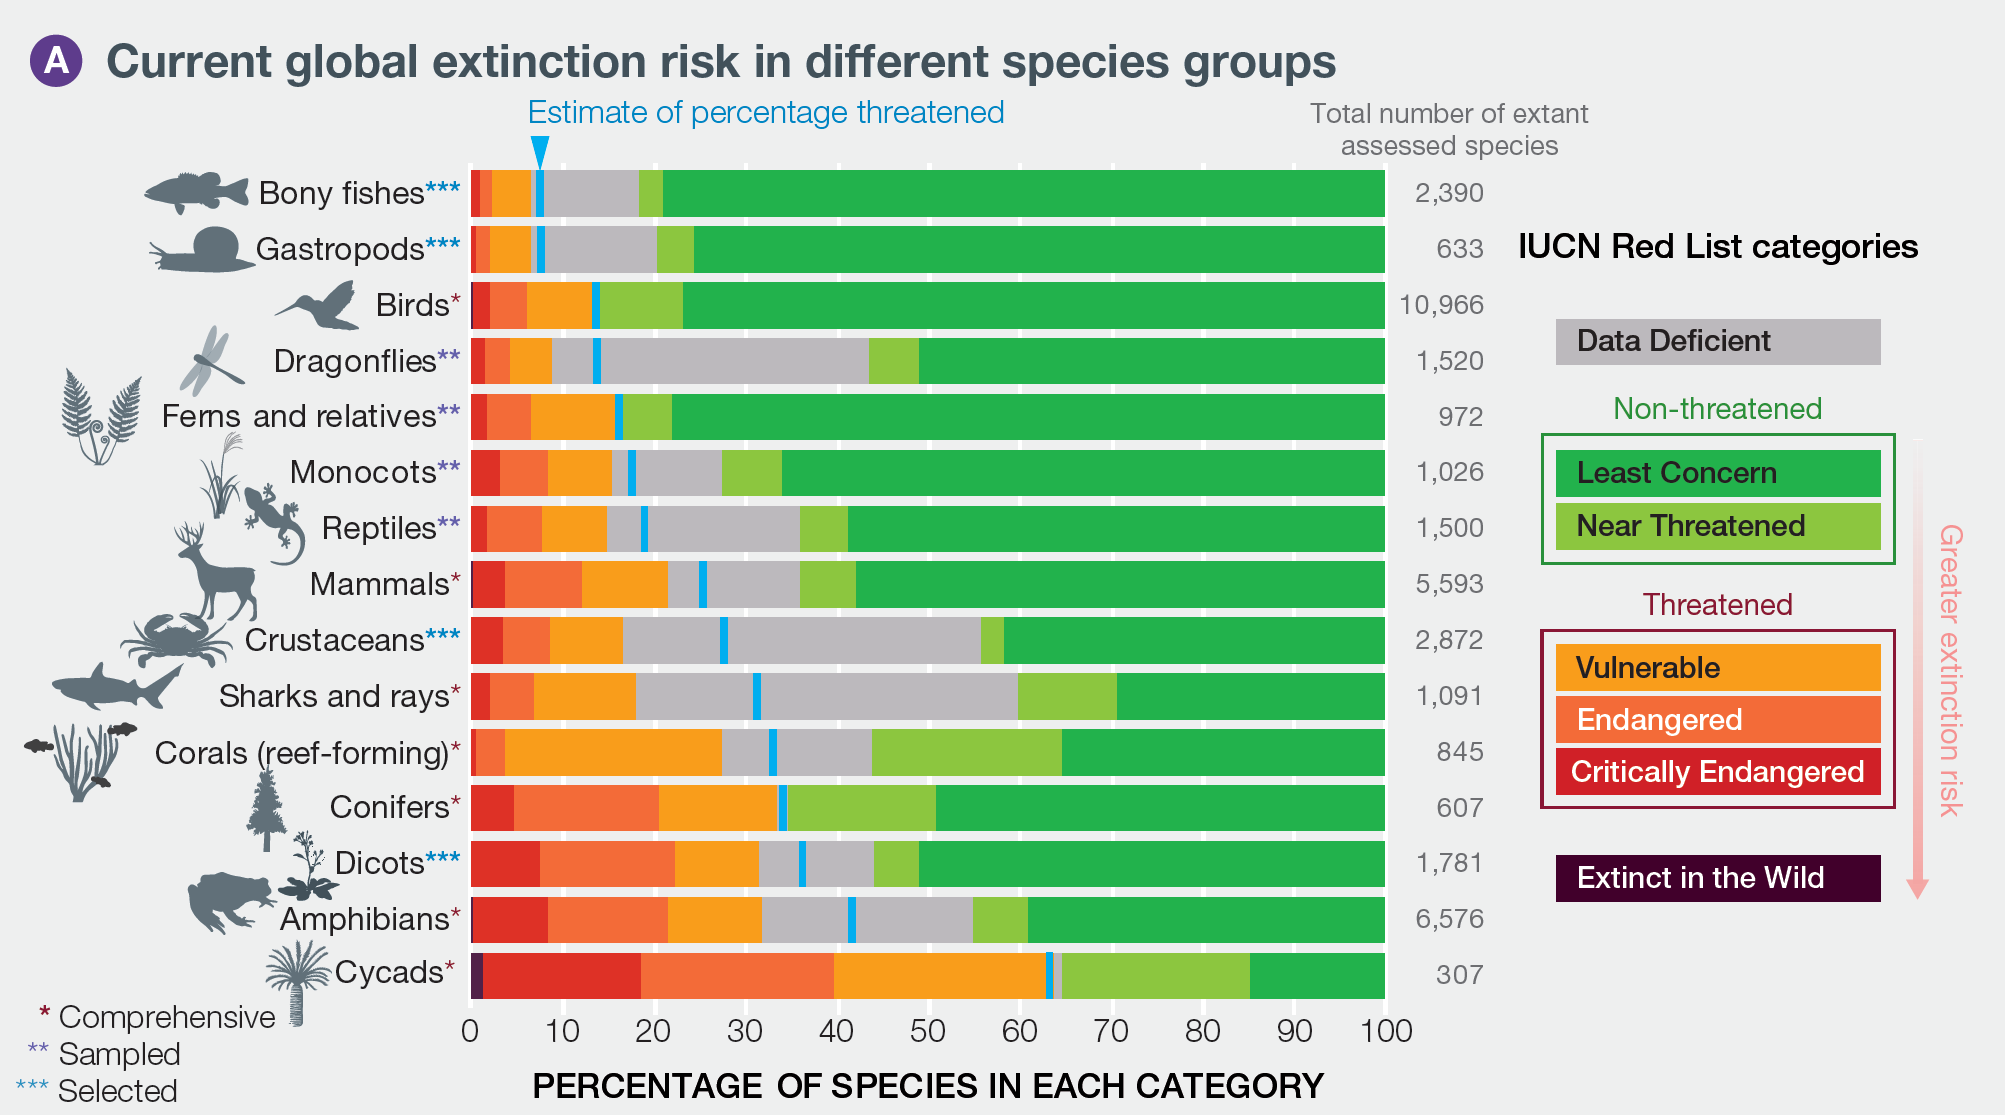
\includegraphics[keepaspectratio]{3_ecological-sustainability/images/Fig3_13__IBPESspecies.png}}

}

\caption{\label{fig-IUCN-red-list}Aktuelles globales Aussterberisiko in
verschiedenen Artengruppen. Quelle: IPBES (2019), Abbildung SPM3}

\end{figure}%

\end{tcolorbox}

Trotz solcher internationaler Bemühungen steht die globale Biodiversität
unter einem beispiellosen Druck. Dies ist auf direkte und indirekte
\textbf{Treiber} (Abbildung~\ref{fig-drivers-biodiversity-loss})
zurückzuführen, die sich in den letzten 50 Jahren erheblich beschleunigt
haben (IPBES 2019, p.25). So haben menschliche Aktivitäten wie
\textbf{Landnutzungsveränderungen} natürliche Lebensräume drastisch
verändert und verkleinert, was zu einem erheblichen Verlust an Arten und
genetischer Vielfalt geführt hat (Pereira u.~a. 2010). Darüber hinaus
ist der Artenverlust auch eng mit dem anthropogenen \textbf{Klimawandel}
verknüpft (vgl. Kapitel), da steigende Temperaturen viele Gebiete und
Regionen für bestimmte Arten unbewohnbar machen bzw. machen werden (WWF
2022, p.16). Dieser Rückgang gefährdet nicht nur die Stabilität der
Ökosysteme, sondern letztlich auch die langfristige Nachhaltigkeit
menschlicher Gesellschaften (Cardinale u.~a. 2012).

\begin{figure}[H]

\centering{

\pandocbounded{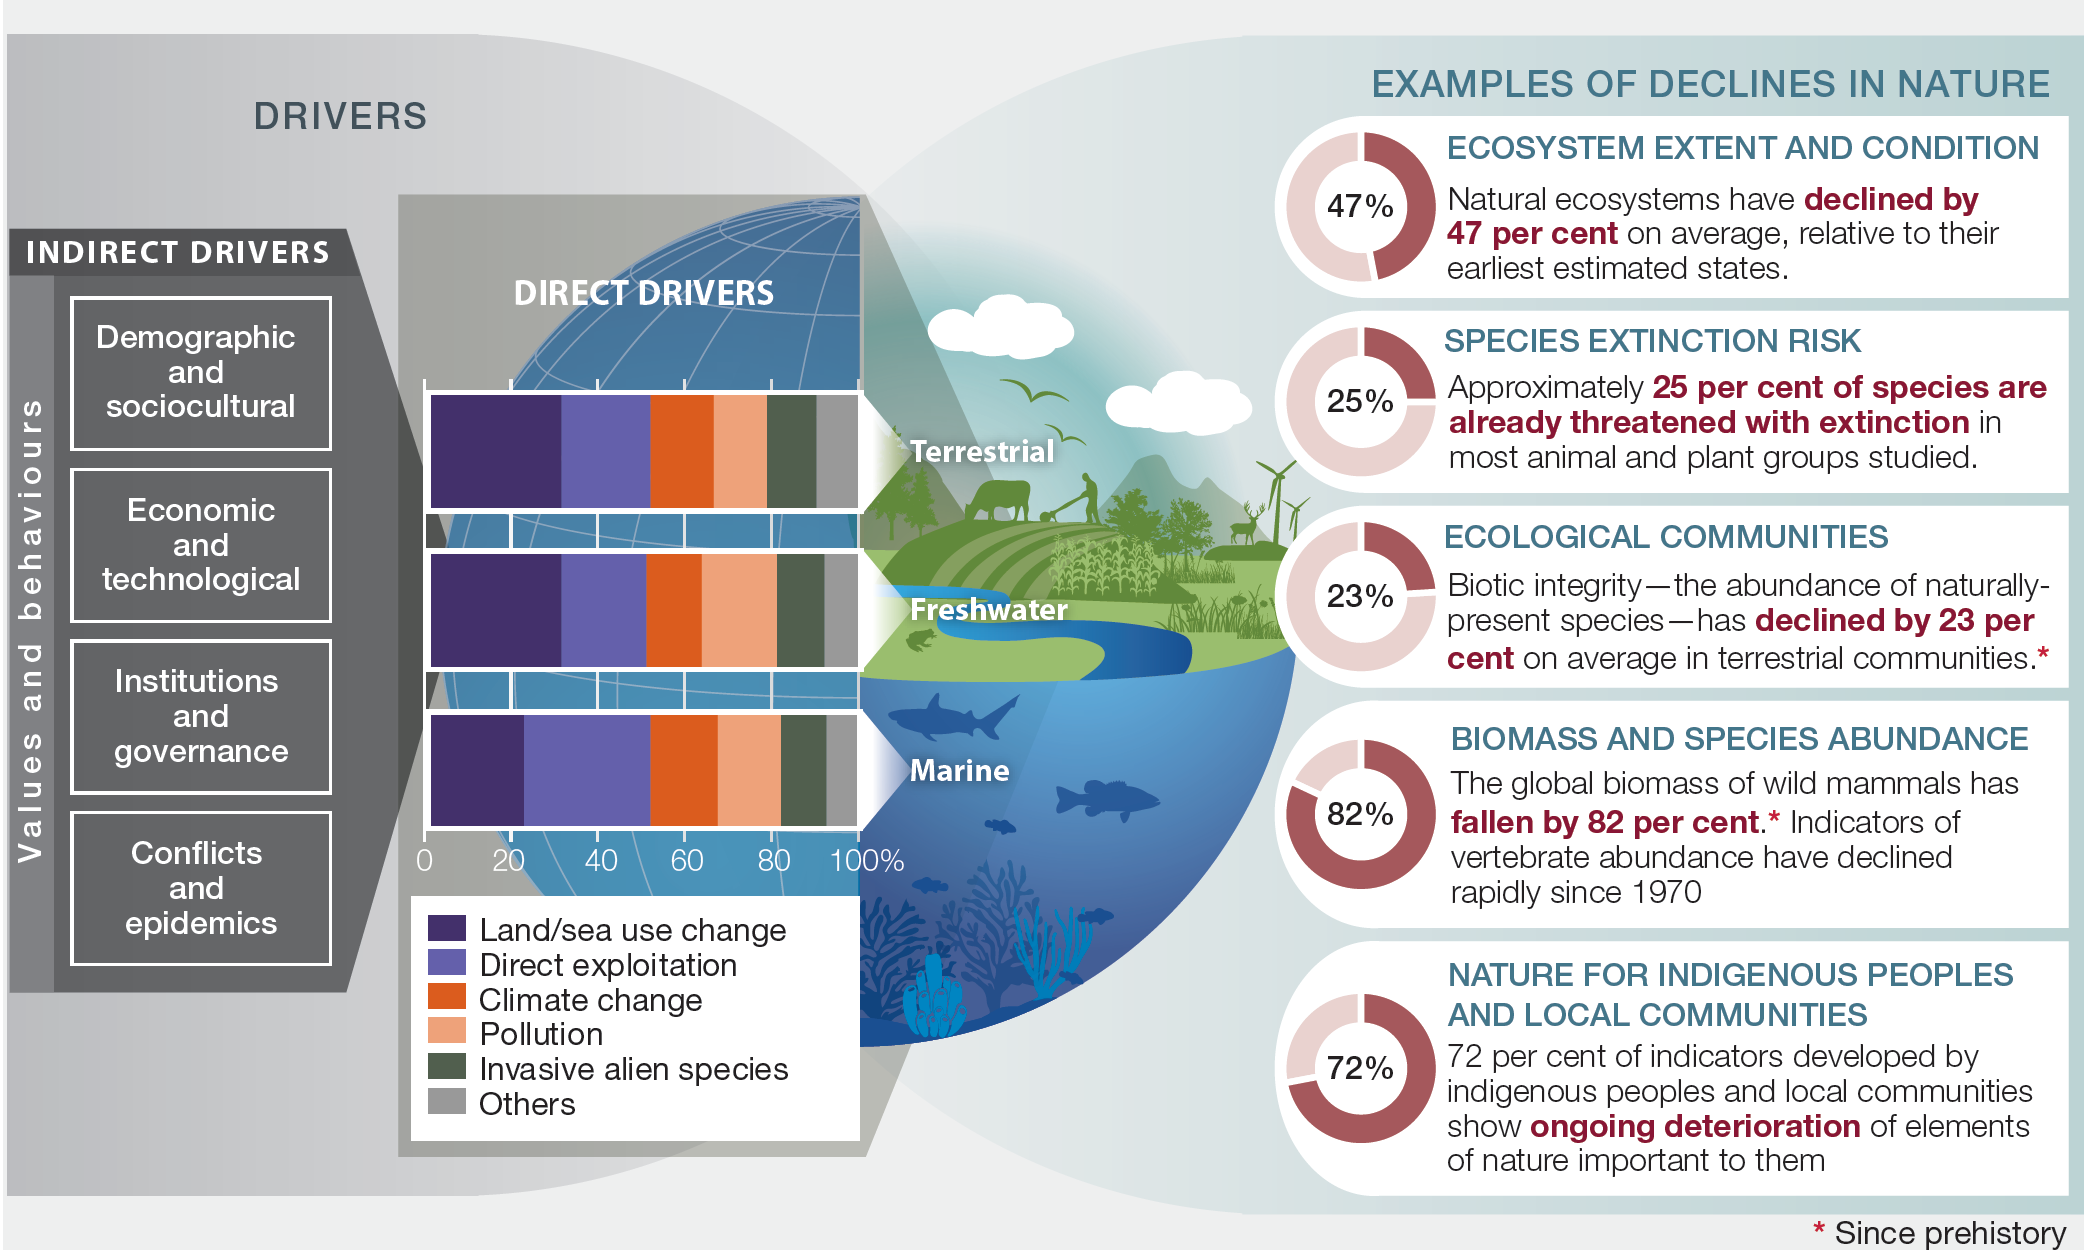
\includegraphics[keepaspectratio]{3_ecological-sustainability/images/Fig3_14__IPBESdrivers.png}}

}

\caption{\label{fig-drivers-biodiversity-loss}Beispiele für den globalen
Rückgang der Natur, der den Biodiversitätsverlust hervorhebt und durch
direkte und indirekte Veränderungstreiber verursacht wurde und wird.
Quelle: IPBES (2019), Abbildung SPM2}

\end{figure}%

Das jüngste wichtige internationale Abkommen, der Globale
Biodiversitätsrahmen Kunming-Montreal (UNEP-CBD 2022), setzt neue Ziele
und Vorgaben (Abbildung~\ref{fig-global-biodiversity-frame}), die den
globalen Biodiversitätsschutz fokussierter gestalten sollen. Ein
zentrales Ziel ist Ziel 3, das festlegt, dass bis 2030 mindestens 30\%
aller Land- und Meeresgebiete, insbesondere solche mit hoher
ökologischer Bedeutung, durch ein System von \emph{Schutzgebieten}
bewahrt werden müssen. Studien haben gezeigt, dass gut verwaltete
Schutzgebiete die Biodiversität wirksam erhalten können. Allerdings
waren bis 2024 nur 16,32\% der terrestrischen Flächen und 8,35\% der
Meeresgebiete geschützt (Protected Planet 2025). Radikalere Ansätze
fordern sogar 50\% Schutzgebiete (das \emph{Half Earth Project}).

\begin{figure}[H]

\centering{

\pandocbounded{\includegraphics[keepaspectratio]{3_ecological-sustainability/images/Fig3_15__KunmingMOntreal.jpg}}

}

\caption{\label{fig-global-biodiversity-frame}Globaler
Biodiversitätsrahmen. Quelle: UNEP-CBD (2022)}

\end{figure}%

Studien und Wissenschaftler*innen haben jedoch Bedenken hinsichtlich der
Wirksamkeit und der (Umwelt-)Gerechtigkeit von \textbf{Schutzgebiets-
und Half-Earth-Ansätzen} geäussert (vgl. Büscher u.~a. 2017; Schleicher
u.~a. 2019). Trotz einer Zunahme der von Schutzgebieten bedeckten Fläche
in den letzten Jahrzehnten nimmt die Biodiversität weiterhin ab.
Einerseits können prozentbasierte Ziele falsche Anreize setzen, indem
Regierungen dazu verleitet werden, Naturschutzgebiete in Gebieten
auszuweisen, in denen sie wenig Nutzen bringen oder nur als Papiertiger
dienen (Visconti u.~a. 2019). Andererseits entzieht die Ausweisung
strenger Schutzgebiete lokalen Bevölkerungsgruppen, insbesondere
indigenen Gruppen, oft den Zugang zu den Gebieten, auf die sie für ihren
Lebensunterhalt angewiesen sind -- oder sie zwingt sie zur Umsiedlung.
Studien haben gezeigt, dass die Beteiligung lokaler Bevölkerungsgruppen
ein entscheidender Faktor für den langfristigen Erhalt und die
Integrität von Schutzgebieten und damit der Biodiversität ist (Andrade
und Rhodes 2012). IPBES (2019, p.32) erkennt ebenfalls die Bedeutung
indigener und lokaler Gemeinschaften für den Schutz von Biodiversität
und Ökosystemdienstleistungen an. Eine Studie von Fa u.~a. (2020)
beispielsweise zeigt, wie die Einbeziehung indigener Gemeinschaften dem
Naturschutz zugutekommen kann. Die Studie zeigt, dass indigene
Territorien weltweit -- und insbesondere in den Tropen -- eine
entscheidende Rolle beim Schutz der Biodiversität und der Eindämmung der
Entwaldung spielen. Die Studie vergleicht die Entwaldungsraten in
verschiedenen Schutzgebieten und zeigt, dass die Entwaldung in Gebieten
unter indigener Verwaltung deutlich geringer ist als in staatlich
geschützten Regionen.

\begin{tcolorbox}[enhanced jigsaw, arc=.35mm, bottomrule=.15mm, bottomtitle=1mm, breakable, colback=white, colbacktitle=quarto-callout-note-color!10!white, colframe=quarto-callout-note-color-frame, coltitle=black, left=2mm, leftrule=.75mm, opacityback=0, opacitybacktitle=0.6, rightrule=.15mm, title={Was ist IPBES?}, titlerule=0mm, toprule=.15mm, toptitle=1mm]

Die Zwischenstaatliche Plattform für Biodiversität und
Ökosystemdienstleistungen (IPBES) ist ein unabhängiges
zwischenstaatliches Gremium, das von verschiedenen Ländern gegründet
wurde, um die Wissenschaft-Politik-Schnittstelle für Biodiversität und
Ökosystemdienstleistungen zugunsten der Erhaltung und nachhaltigen
Nutzung der Biodiversität, des langfristigen menschlichen Wohlergehens
und der nachhaltigen Entwicklung zu stärken. Sie wurde am 21. April 2012
in Panama-Stadt von 94 Regierungen gegründet. Die Sekretariatsleistungen
für IPBES werden vom Umweltprogramm der Vereinten Nationen (UNEP)
erbracht, obwohl IPBES kein UN-Organ ist. Heute gilt IPBES, das das
NCP-Konzept entwickelt hat, als Gegenstück zum IPCC (IPBES secretariat
2017).

\end{tcolorbox}

Wie Landnutzungsveränderungen (Verweis) und Ökosystemdienstleistungen
(Verweis) sind auch Biodiversitätsschutz und Naturschutz in verschiedene
\textbf{Werte und Visionen} eingebettet, die zu Interessenkonflikten
zwischen verschiedenen Stakeholdern führen können. Diese Werte und die
daraus resultierenden Ansätze werden in der Regel in drei Typen
unterteilt: intrinsische, instrumentelle und relationale Werte (Durán
u.~a. 2023): mit anderen Worten, „Natur um ihrer selbst willen'', „Natur
als Kultur'' und „Natur für die Gesellschaft''
(Abbildung~\ref{fig-NFF}). Das Konzept der Ökosystemdienstleistungen
beispielsweise fällt unter „\textbf{Natur für die Gesellschaft}'', da es
einer utilitaristischen Sichtweise der Natur entspricht, bei der die
Gesellschaft den grösstmöglichen Nutzen aus der Natur zieht (ohne ihr zu
schaden). Im Gegensatz dazu kann ein Naturpark, der strengen Naturschutz
oder die Rewilding von Gebieten priorisiert, als Verkörperung
intrinsischer Werte eingestuft werden, weil menschliche Eingriffe und
damit die Auswirkungen auf die Natur minimiert werden. Diese
„\textbf{Natur um ihrer selbst willen}''-Erzählung erstreckt sich auch
auf Konzepte wie Smart Cities, da diese darauf abzielen, menschliche
Aktivitäten so effizient wie möglich auf städtische Gebiete zu
beschränken. Die Vision „\textbf{Natur als Kultur}'' stellt eine Welt
dar, in der Werte wie Gegenseitigkeit und Harmonie die menschlichen
Beziehungen zur Natur auf allen Ebenen definieren. Hier werden
biologische Vielfalt und kulturelle Vielfalt gemeinsam in eng
verknüpften biokulturellen Systemen bewahrt und gepflegt. Diese Systeme
werden von lokalen, selbstbestimmten Governance-Strukturen getragen, die
die indigene Souveränität und lokale Identitäten respektieren. Der
wirtschaftliche Austausch priorisiert den sozialen Wert von Gütern
gegenüber ihrem monetären Wert. Diese Vision umfasst beispielsweise
lokale und dezentralisierte Nahrungsmittelproduktion sowie
Gemeinschaften, die in einem resilienten, biokulturellen Netzwerk mit
tiefen spirituellen Verbindungen zur Natur operieren.

\begin{figure}[H]

\centering{

\pandocbounded{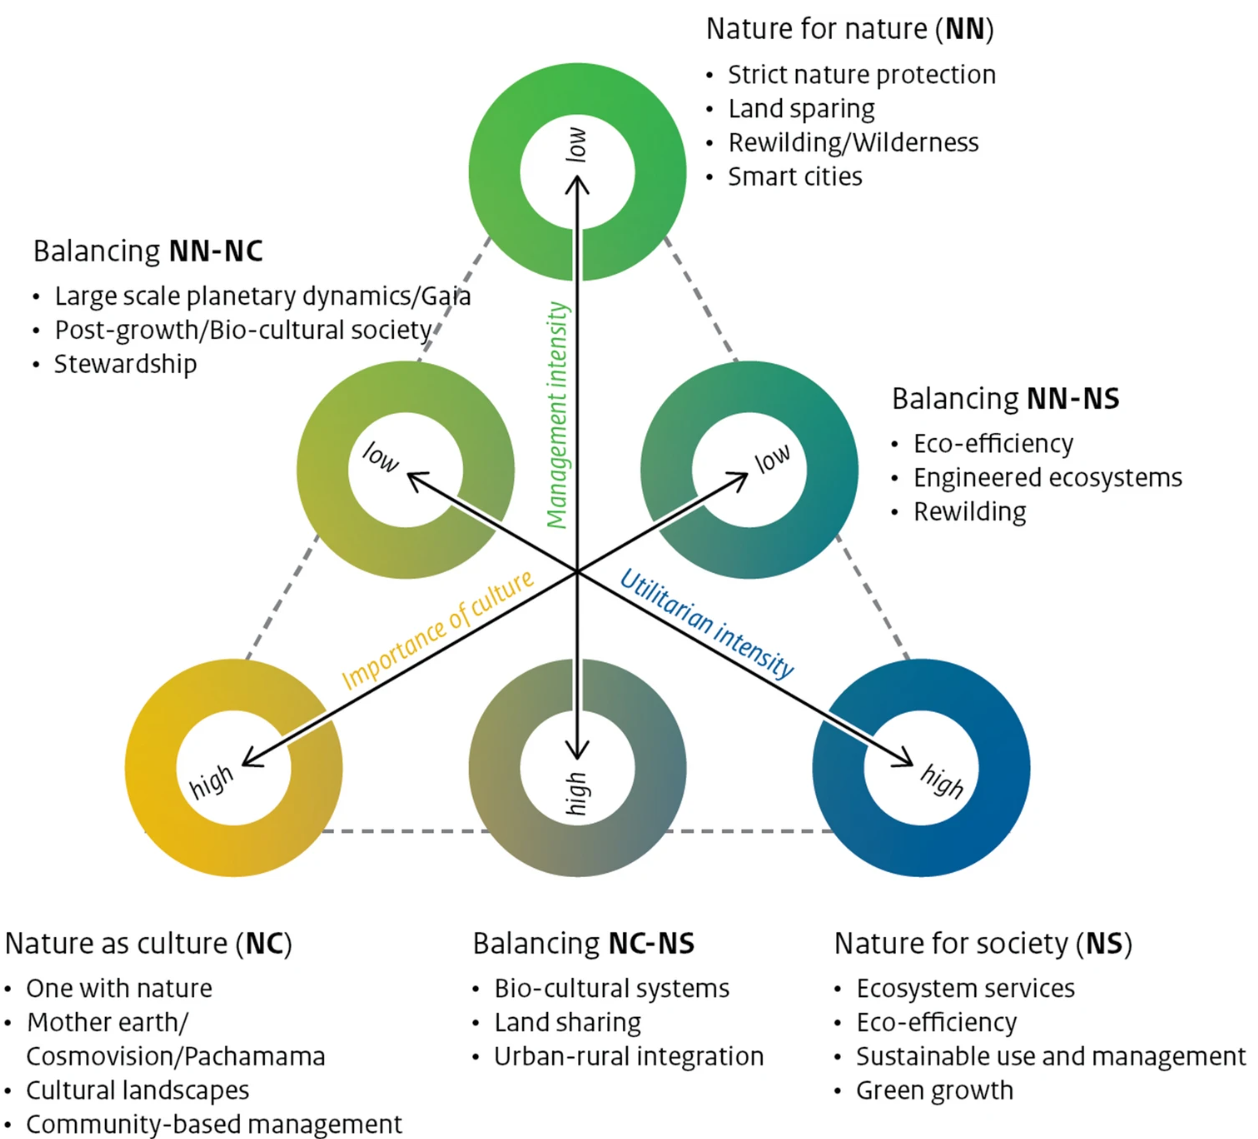
\includegraphics[keepaspectratio]{3_ecological-sustainability/images/Fig3_16__NatureFuturesFramework.png}}

}

\caption{\label{fig-NFF}Das Nature Futures Framework (NFF) und die drei
wichtigsten Perspektiven auf den Naturschutz. Quelle: Durán u.~a.
(2023), basierend auf {Pereira u.~a.} (2020). Creative Commons CC BY
4.0.}

\end{figure}%

Die unterschiedlichen Werte, die mit Biodiversität und Natur verknüpft
sind -- und in welchem Umfang sie geschützt werden sollten --, erfordern
daher eine normative Beurteilung. Sie basieren nicht nur auf empirischem
Systemwissen, sondern auch auf ethischen Grundsätzen, wie zu Beginn von
Kapitel 3 erläutert.

Wie wir gesehen haben, und wie bei anderen
Nachhaltigkeitsherausforderungen und -dimensionen, gibt es keinen
etablierten Konsens darüber, wie Nachhaltigkeit in der ökologischen
Dimension am besten umgesetzt und erreicht werden kann. Auch in dieser
Dimension bleibt nachhaltige Entwicklung ein gesellschaftlicher
Aushandlungs- und Entscheidungsprozess. Angesichts der Vielfalt
unterschiedlicher Perspektiven und Interessen verschiedener Stakeholder
variieren auch die Präferenzen hinsichtlich Ansätzen und Massnahmen. Um
geeignete Massnahmen auszuwählen und die verschiedenen
Verantwortungsebenen zu harmonisieren (Abbildung~\ref{fig-SD-ethics}),
können wir uns beispielsweise auf Hans Jonas' (1979) Verantwortungsethik
beziehen, die wir zu Beginn des Buches kennengelernt haben. Die
Integration dieser verschiedenen Verantwortungsbereiche kann eine
ganzheitliche und nachhaltige Ethik fördern, die die Bedürfnisse und
Interessen aller Aspekte des Lebens und der Natur angemessen
berücksichtigt.

\begin{figure}[H]

\centering{

\pandocbounded{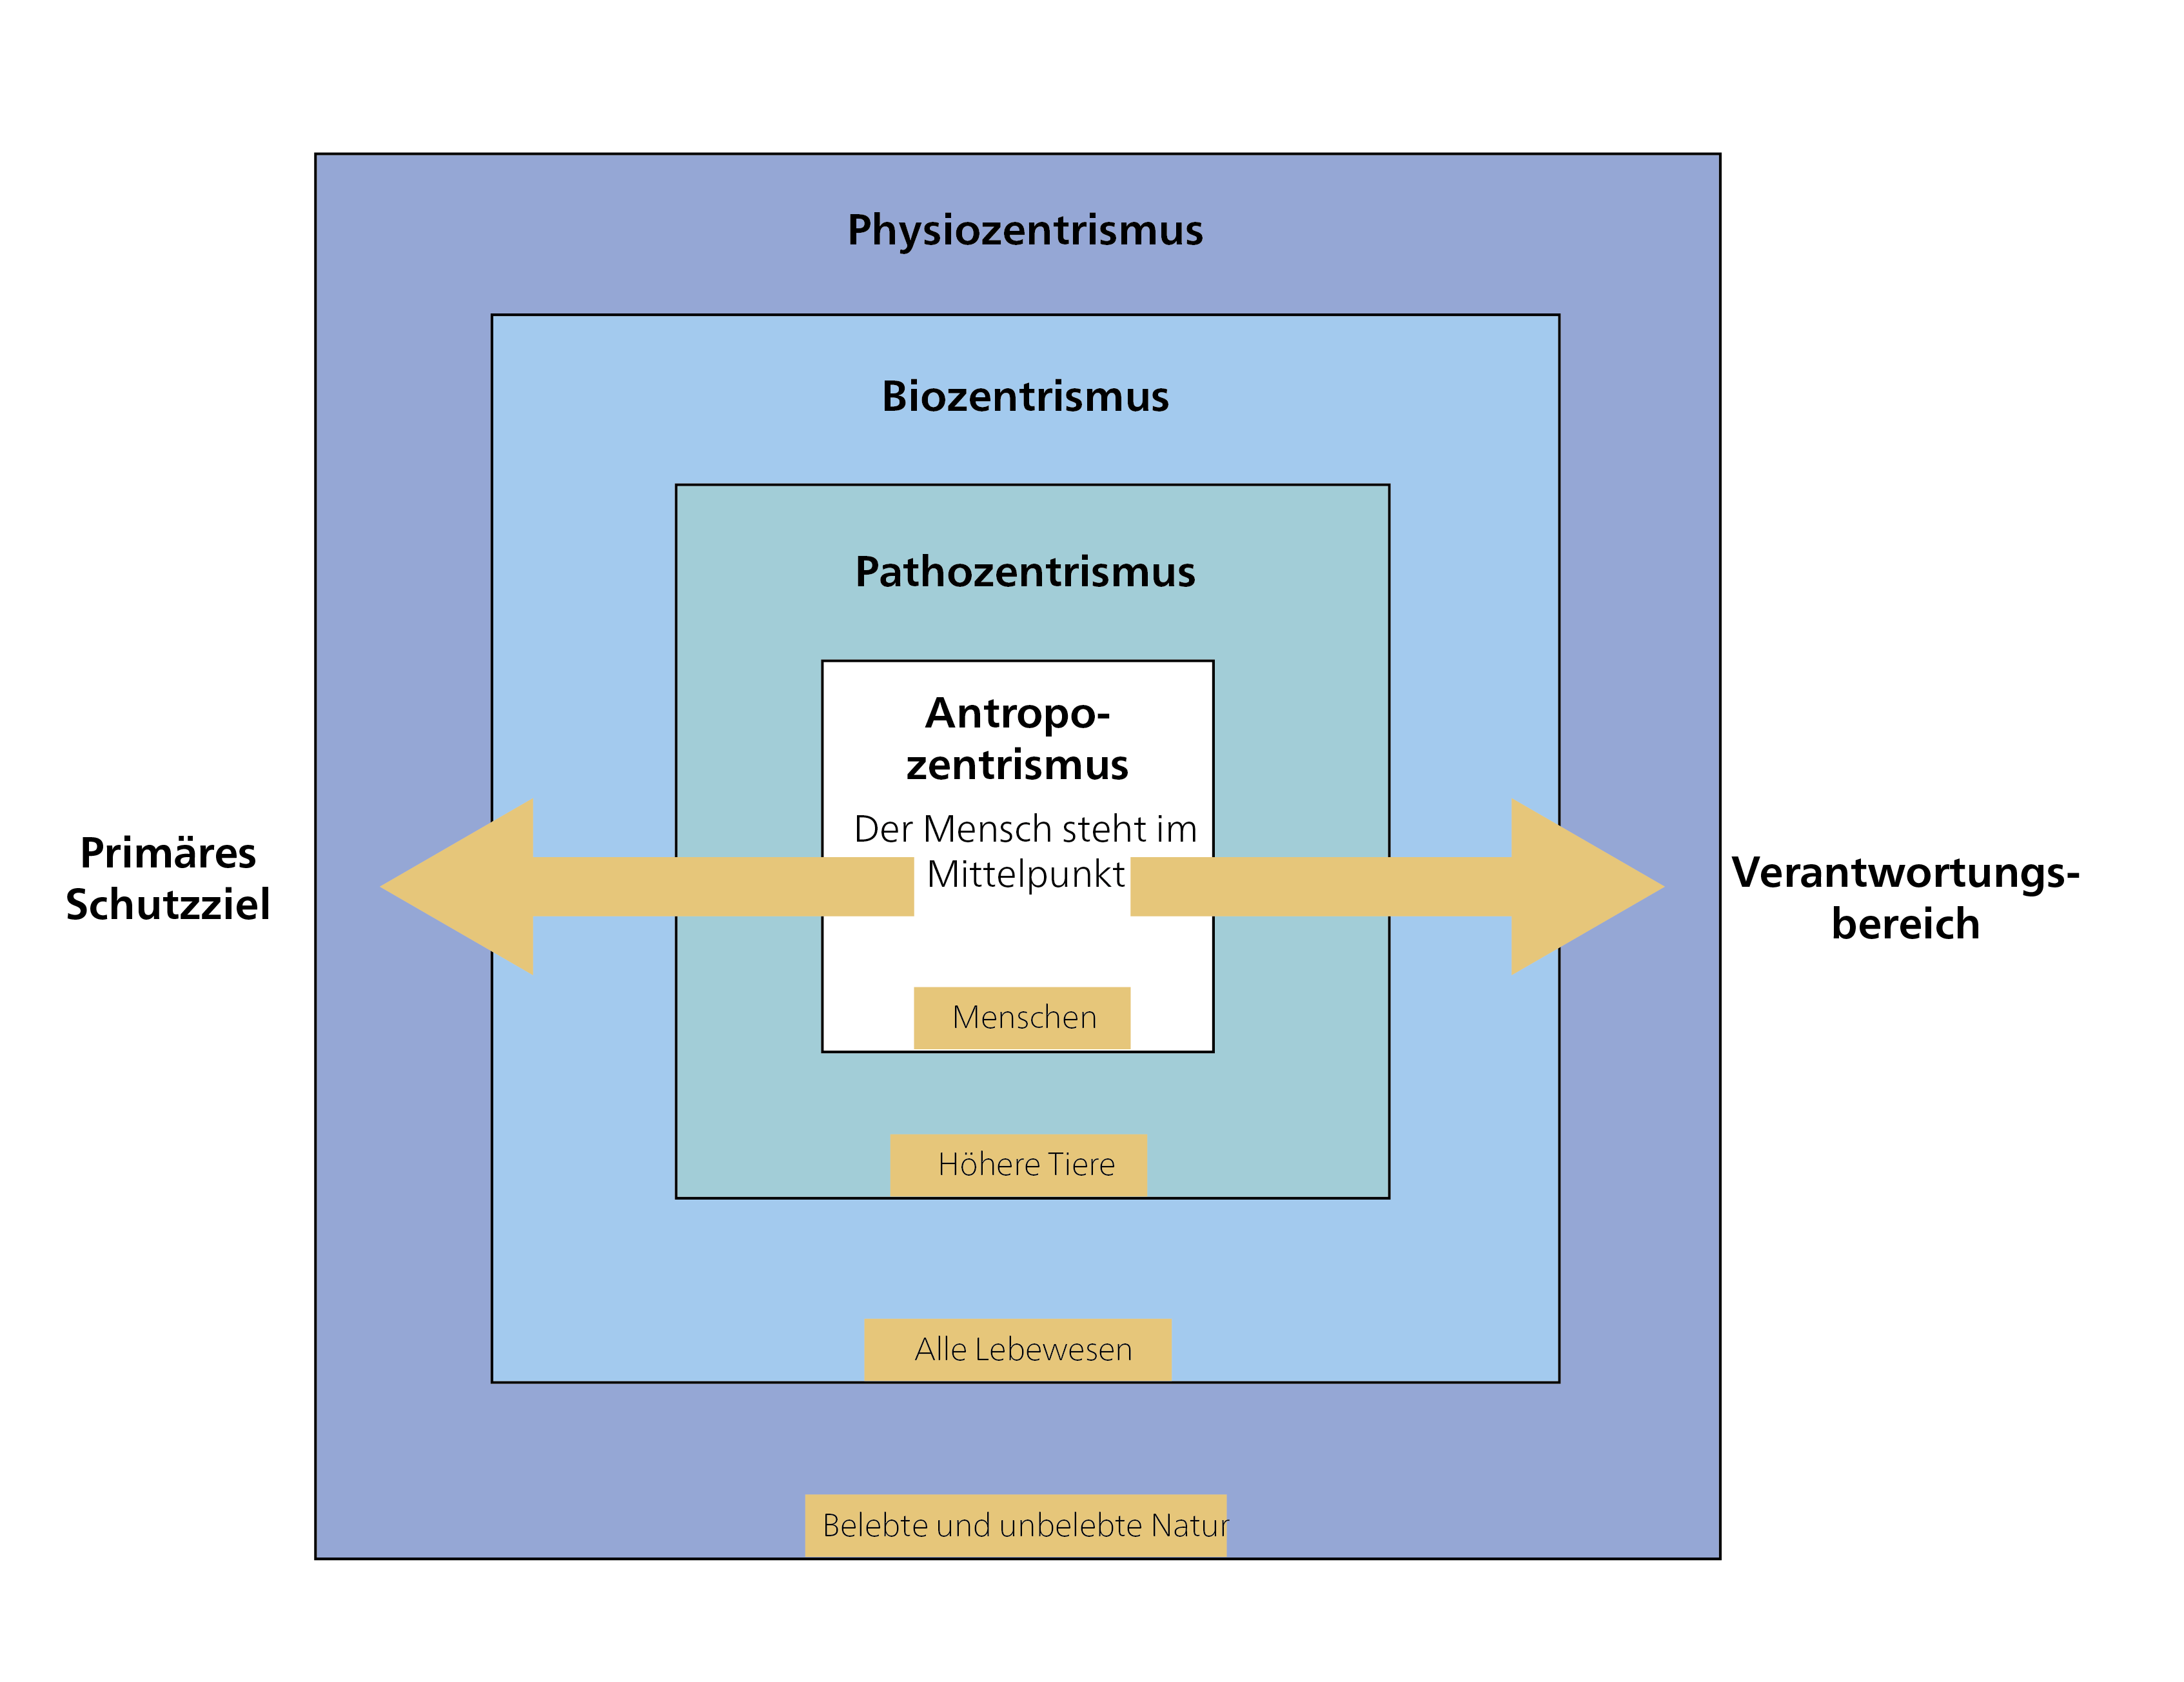
\includegraphics[keepaspectratio]{3_ecological-sustainability/images/Fig3_18_ethik.png}}

}

\caption{\label{fig-SD-ethics}Ethik der Nachhaltigen Entwicklung
(Quelle: Eigene Darstellung)}

\end{figure}%

\section{Strategische Ansätze}\label{strategische-ansuxe4tze}

Heutzutage werden verschiedene Strategien verfolgt oder zumindest in
Betracht gezogen, um eine Transformation in der ökologischen Dimension
der nachhaltigen Entwicklung zu erreichen (vgl. Abbildung~\ref{fig-GDSR}
für eine nicht abschliessende Aufzählung). Einige dieser Strategien
wurden bereits in diesem Lehrbuch besprochen. Obwohl die genannten
Ansätze nicht zwingend per se transformativ sein müssen, können sie bei
geeigneter Anwendung durchaus Auswirkungen auf die ökologische Dimension
der Nachhaltigkeit haben. Die in diesem Abschnitt vorgestellten Ansätze
werden gemäss den „Hebeln für die Transformation'' des Global
Sustainable Development Report (GSDR) kategorisiert. Der GSDR 2019
definiert vier Hebel: Governance, Wirtschaft und Finanzen, individuelle
und kollektive Handlungen sowie Wissenschaft und Technologie. Der GSDR
2023 fügte einen fünften Hebel hinzu -- Kapazitätsaufbau --, da dieser
sowohl als Hebel selbst als auch als unterstützender Faktor für die
anderen Hebel für einen transformativen Prozess unerlässlich ist
(Independent Group of Scientists appointed by the Secretary-General
2023).

\begin{figure}[H]

\centering{

\pandocbounded{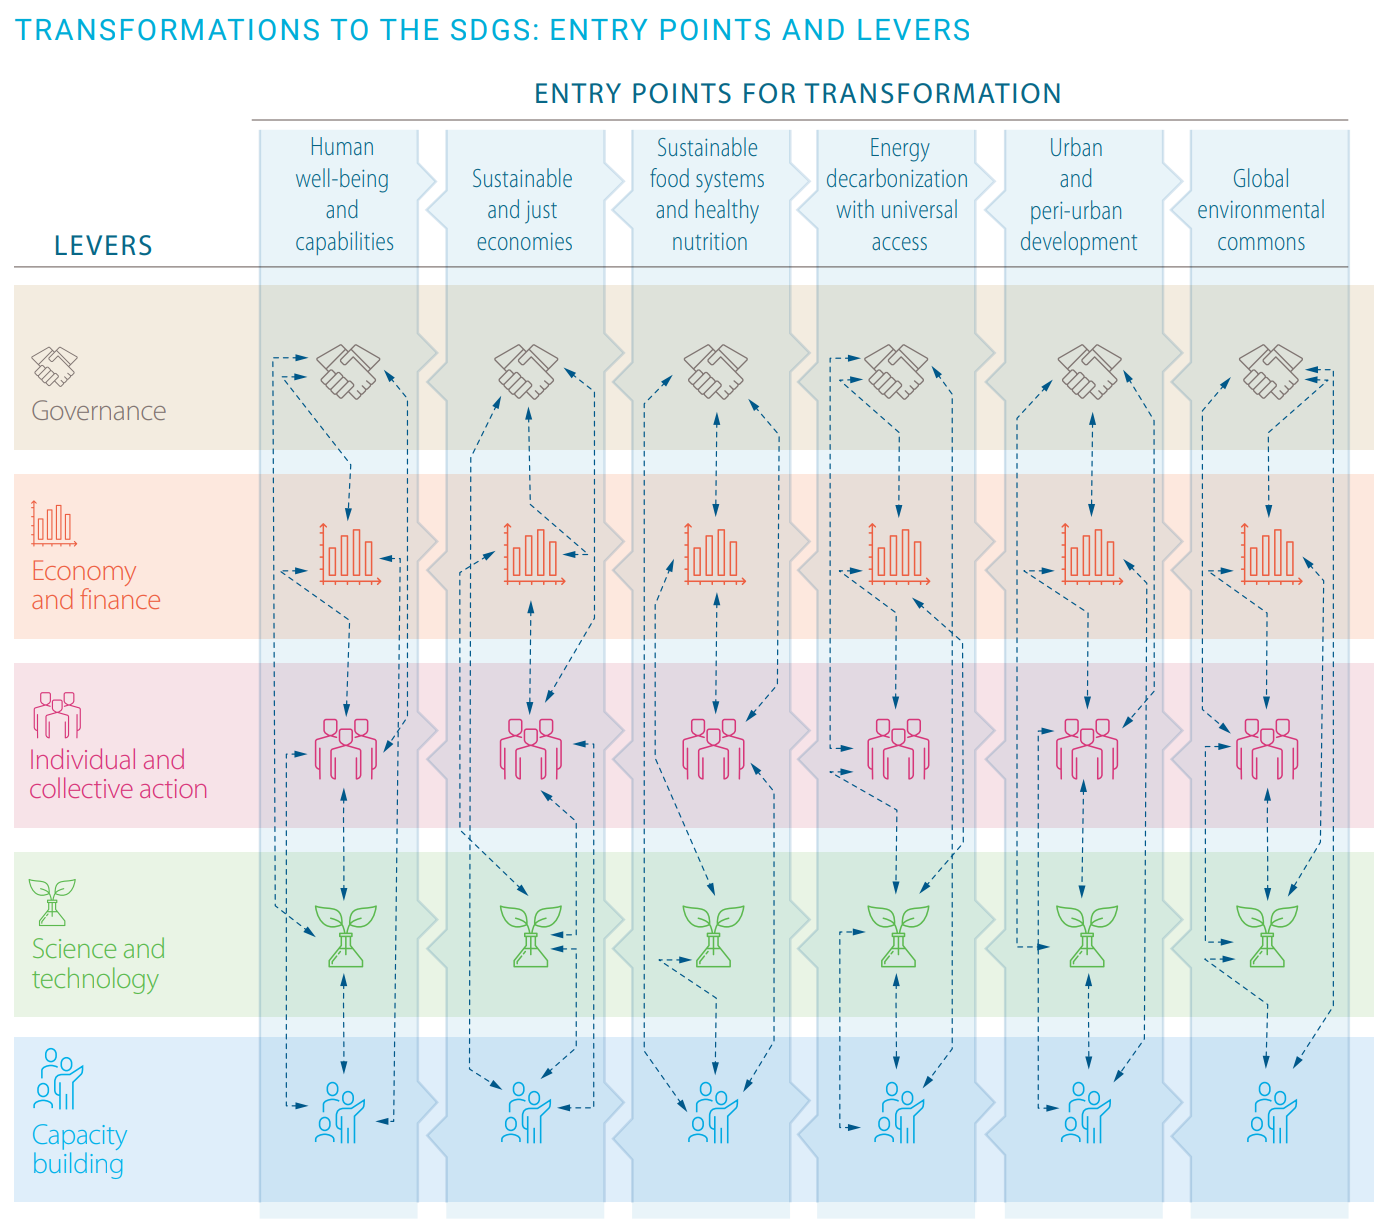
\includegraphics[keepaspectratio]{3_ecological-sustainability/images/Fig3_17__GSDR.png}}

}

\caption{\label{fig-GDSR}Transformationsmodell zur Erreichung der Ziele
für nachhaltige Entwicklung (SDGs) gemäss dem Global Report of
Sustainable Development 2023. Quelle: Gong (2024), lizenziert unter CC
BY-NC-SA 4.0}

\end{figure}%

Für jeden Hebel stellen wir ausgewählte Strategien vor, die mit unseren
drei Schwerpunktthemen in diesem Kapitel -- Klima, Landnutzung oder
Biodiversität -- zusammenhängen:

Der \textbf{Governance}-Hebel umfasst Institutionen und Räume, die die
Entwicklungsrichtung bestimmen, indem sie Ziele setzen, Massnahmen
koordinieren, Regulierungen schaffen und die Finanzierung auf nationaler
und regionaler Ebene erleichtern. Gute Governance sollte auch Synergien
fördern, Interessenkonflikte berücksichtigen und die Zusammenarbeit
zwischen einem breiten Spektrum von Stakeholdern stärken. Governance
spielt damit eine Schlüsselrolle bei der Entwicklung und Umsetzung von
Strategien zur ökologischen Nachhaltigkeit, da sie den politischen
Rahmen für nachhaltige Praktiken durch regulatorische Mechanismen,
Anreizstrukturen und Gesetze schaffen kann. Zu den Governance-Hebeln
gehören:

\begin{itemize}
\item
  Schaffung von Schutzgebieten zur Erhaltung der Biodiversität
\item
  Subventionen für nachhaltige Praktiken, wie Direktzahlungen für
  biodiversitätsfreundliche Bewirtschaftungsmethoden
\end{itemize}

Der Hebel \textbf{Wirtschaft und Finanzen} bezieht sich in erster Linie
auf die erheblichen öffentlichen und privaten Investitionen, die zur
Erreichung der SDGs und der Transformation erforderlich sind (global
zwischen 1,4 und 2,5 Billionen US-Dollar pro Jahr). Dieser Hebel ist
damit ein wichtiger Ermöglicher von Strategien und Politiken zur
ökologischen Nachhaltigkeit, beispielsweise durch die Finanzierung
nachhaltiger Technologien. Beispiele umfassen:

\begin{itemize}
\item
  Zahlungen für Ökosystemdienstleistungen (PES)
\item
  REDD+-Programme zur Reduzierung von Entwaldung und zur Förderung
  nachhaltiger Landnutzung
\end{itemize}

Der Hebel \textbf{Wissenschaft und Technologie} bezieht sich auf soziale
und technologische Innovationen sowie auf kosteneffektive und
skalierbare Technologien. Dazu gehören Investitionen in Forschung und
Entwicklung, die Förderung einer stärkeren internationalen
Zusammenarbeit und die Ermöglichung des Zugangs zu bewährten
Technologien (insbesondere für Länder mit niedrigem Einkommen).
Wissenschaft kann dabei helfen, komplexe Zusammenhänge zu erklären und
evidenzbasierte Lösungen zu entwickeln. Wesentliche Hebel für
Nachhaltigkeitstransformationen umfassen:

\begin{itemize}
\item
  Technologien zur Kohlenstoffbindung
\item
  Naturbasierte Lösungen, die natürliche Prozesse nutzen, um dem
  Klimawandel und Umweltproblemen zu begegnen
\item
  Innovative Landnutzungssysteme, wie Agroforstwirtschaft
\end{itemize}

\textbf{Individuelle und kollektive Handlungen}\\
Sozialer Wandel beginnt oft in den Herzen und Köpfen der Menschen durch
lokale Organisation und Mobilisierung, bevor er sich in Gesetze und
Wirtschaftspolitik übersetzt. Wenn eine kritische Masse neue Praktiken
oder Normen annimmt, kann dies durch Bildung, Informationskampagnen,
finanzielle Anreize und Gesetzgebung unterstützt und auf die gesamte
Gesellschaft ausgedehnt werden. Beispiele für Nachhaltigkeitsstrategien
und -politiken im Bereich der individuellen und kollektiven Handlungen
umfassen:

\begin{itemize}
\item
  Kampagnen für nachhaltigen Konsum, die Konsument*innen motivieren,
  umweltfreundliche Produkte zu wählen
\item
  Förderung solidarischer Landwirtschaftsmodelle (SoLaWi), die die
  regionale und ökologische Nahrungsmittelproduktion stärken
\end{itemize}

\textbf{Kapazitätsaufbau}\\
Der Kapazitätsaufbau zur Unterstützung der Transformation zur Erreichung
der SDGs ist vielschichtig und hängt von den Zielen, den erforderlichen
Transformationen sowie dem spezifischen Landes- oder Regionalkontext ab.
Unter anderem sind Kompetenzen in den Bereichen strategische
Ausrichtung, Innovation, Koordination, Lernen und Resilienz
erforderlich. Zu den Strategien und Politiken zur ökologischen
Nachhaltigkeit im Zusammenhang mit dem Kapazitätsaufbau-Hebel gehören:

\begin{itemize}
\item
  Einrichtung von Beratungszentren oder digitalen Plattformen zur
  Ermöglichung kontinuierlichen Lernens und des Austauschs bewährter
  Praktiken, z. B. im Bereich der Agroforstwirtschaft
\item
  Unterstützung lokaler Initiativen zur Verbesserung des
  Wissenstransfers
\end{itemize}

Hinweis: Es ist wichtig zu beachten, dass Ansätze nicht immer
synergetisch sind; oft gehen Ansätze, die eine ökologische Dimension der
Nachhaltigkeit adressieren, mit Zielkonflikten mit anderen Ansätzen oder
mit der sozialen oder wirtschaftlichen Dimension der Nachhaltigkeit
einher.

\begin{tcolorbox}[enhanced jigsaw, arc=.35mm, bottomrule=.15mm, bottomtitle=1mm, breakable, colback=white, colbacktitle=quarto-callout-caution-color!10!white, colframe=quarto-callout-caution-color-frame, coltitle=black, left=2mm, leftrule=.75mm, opacityback=0, opacitybacktitle=0.6, rightrule=.15mm, title={Weiterführende Literatur}, titlerule=0mm, toprule=.15mm, toptitle=1mm]

\begin{itemize}
\tightlist
\item
  Guyer, Madeleine, Myriam Steinemann, and Nina Saalismaa. 2022.
  \emph{Biodiversity and Sustainable Development}. Climate Change \&
  Environment Nexus Brief. Swiss Agency for Development and Cooperation.
\end{itemize}

\end{tcolorbox}

\section{Grundlagen der Nachhaltigkeit: Das Quiz -- Kapitel
3}\label{grundlagen-der-nachhaltigkeit-das-quiz-kapitel-3}

Welche der folgenden Aussagen zum Konzept der Ökosystemdienstleistungen
sind korrekt? (Mehr als eine Aussage kann richtig sein.)

\begin{itemize}
\tightlist
\item[$\square$]
  Das Konzept der Ökosystemdienstleistungen bezeichnet die direkten und
  indirekten Vorteile, die Menschen aus Ökosystemen ziehen.
\item[$\square$]
  Das Konzept der Ökosystemdienstleistungen ist ein Mass für
  Biodiversität und damit auch ein Mass für die Resilienz eines
  Ökosystems.
\item[$\square$]
  Im Gegensatz zum Konzept der Nachhaltigen Entwicklung ist das Konzept
  der Ökosystemdienstleistungen nicht anthropozentrisch, sondern
  ökozentrisch.
\item[$\square$]
  Das Konzept der Ökosystemdienstleistungen umfasst alle Massnahmen, die
  Menschen zur Erhaltung von Ökosystemen ergreifen.
\item[$\square$]
  Es lassen sich vier Arten von Ökosystemdienstleistungen unterscheiden:
  Regulierungsdienstleistungen, Versorgungsdienstleistungen, kulturelle
  Dienstleistungen und Unterstützungsdienstleistungen.
\item[$\square$]
  Es lassen sich drei Arten von Ökosystemdienstleistungen unterscheiden:
  Vermeidungs-, Verbesserungs- und Verlagerungsdienstleistungen.
\item[$\square$]
  Der Begriff „Ökosystemdienstleistungen'' ist ein wissenschaftlicher
  Begriff, der die Zusammenkünfte naturbezogener Religionen (sogenannter
  Naturreligionen) wie des Animismus beschreibt, bei denen die Natur als
  Ganzes verehrt wird.
\item[$\square$]
  Das Konzept der Ökosystemdienstleistungen bezeichnet die jährliche
  Biomasseanhäufung innerhalb eines Ökosystems, gemessen in Kilojoule.
\end{itemize}

Das Konzept der Ökosystemdienstleistungen bezeichnet die direkten und
indirekten Vorteile, die Menschen aus Ökosystemen ziehen, und ist damit
ausdrücklich anthropozentrisch. Eine gängige Klassifikation
unterscheidet vier Arten von Ökosystemdienstleistungen: Versorgungs-,
Regulierungs-, kulturelle und Unterstützungsdienstleistungen. Die
übrigen Aussagen verwechseln Ökosystemdienstleistungen mit
Biodiversitätsmassen, ökologischen Produktivitätsmassen,
Schutzmassnahmen, alternativen Klassifikationen oder unverwandten
kulturellen bzw. religiösen Konzepten.

\begin{itemize}
\tightlist
\item
  True
\item
  False
\item
  False
\item
  False
\item
  True
\item
  False
\item
  False
\item
  False
\end{itemize}

Was sind die vier Hauptkategorien von Ökosystemdienstleistungen?

\begin{itemize}
\tightlist
\item[$\square$]
  Materielle, spirituelle, industrielle und soziale Dienstleistungen
\item[$\square$]
  Wirtschaftliche, soziale, ökologische und kulturelle Dienstleistungen
\item[$\square$]
  Versorgungs-, Regulierungs-, kulturelle und
  Unterstützungsdienstleistungen
\end{itemize}

Ökosystemdienstleistungen werden gängigerweise in vier Hauptkategorien
eingeteilt: Versorgungsdienstleistungen (z. B. Nahrung und Rohstoffe),
Regulierungsdienstleistungen (z. B. Klimaregulierung), kulturelle
Dienstleistungen (z. B. Erholung und spirituelle Werte) und
Unterstützungsdienstleistungen (z. B. Nährstoffkreisläufe und
Bodenbildung).

\begin{itemize}
\tightlist
\item
  False
\item
  False
\item
  True
\end{itemize}

Welche der folgenden Aussagen treffen auf das Konzept der
Ökosystemdienstleistungen zu, welche nicht? (Mehr als eine Aussage kann
richtig sein.)

\begin{itemize}
\tightlist
\item[$\square$]
  Ökosystemdienstleistungen lassen sich in folgende Kategorien
  einteilen: Unterstützungs-, Versorgungs-, Regulierungs- und kulturelle
  Dienstleistungen.
\item[$\square$]
  Ökosystemdienstleistungen bezeichnen die direkten und indirekten
  Beiträge von Ökosystemen zum menschlichen Wohlergehen.
\item[$\square$]
  Ökosystemdienstleistungen sind ein Mass für Biodiversität und folglich
  für die Resilienz eines Ökosystems.
\item[$\square$]
  Ökosystemdienstleistungen bezeichnen die jährliche Biomasseanhäufung
  innerhalb eines Ökosystems, gemessen in Kilojoule.
\end{itemize}

Das Konzept der Ökosystemdienstleistungen bezeichnet die direkten und
indirekten Beiträge von Ökosystemen zum menschlichen Wohlergehen und
wird meist in vier Kategorien gegliedert: Versorgungs-, Regulierungs-,
kulturelle und Unterstützungsdienstleistungen. Es dient weder als
direktes Mass für Biodiversität oder Ökosystemresilienz, noch beschreibt
es biophysikalische Produktivitätsmasse wie die jährliche
Biomasseanhäufung.

\begin{itemize}
\tightlist
\item
  True
\item
  True
\item
  False
\item
  False
\end{itemize}

Welche der folgenden sind Arten von Rückkopplungsmechanismen im
Klimasystem? (Mehr als eine Aussage kann richtig sein.)

\begin{itemize}
\tightlist
\item[$\square$]
  Neutrale Rückkopplung
\item[$\square$]
  Negative Rückkopplung
\item[$\square$]
  Positive Rückkopplung
\end{itemize}

Rückkopplungsmechanismen im Klimasystem beschreiben Prozesse, die
Veränderungen im Klimasystem entweder verstärken (positive Rückkopplung)
oder abschwächen (negative Rückkopplung). Neutrale Rückkopplung wird in
der Klimawissenschaft üblicherweise nicht als eigene Kategorie
verwendet.

\begin{itemize}
\tightlist
\item
  False
\item
  True
\item
  True
\end{itemize}

Welche der folgenden sind direkte Treiber des Biodiversitätsverlusts?
(Mehr als eine Aussage kann richtig sein.)

\begin{itemize}
\tightlist
\item[$\square$]
  Umweltverschmutzung
\item[$\square$]
  Wirtschaftspolitik
\item[$\square$]
  Klimawandel
\item[$\square$]
  Landnutzungsveränderungen
\end{itemize}

Direkte Treiber des Biodiversitätsverlusts sind Faktoren, die
unmittelbar auf Ökosysteme und Arten einwirken. Dazu gehören
Landnutzungsveränderungen (z. B. Zerstörung von Lebensräumen),
Umweltverschmutzung und Klimawandel. Wirtschaftspolitik hingegen gilt
als indirekter Treiber, da sie den Biodiversitätsverlust über
sozioökonomische Wirkungspfade beeinflusst und nicht durch direkten
ökologischen Druck.

\begin{itemize}
\tightlist
\item
  True
\item
  False
\item
  True
\item
  True
\end{itemize}

Welche der folgenden Aussagen beschreiben Landnutzungsveränderungen und
verwandte Konzepte korrekt? (Mehr als eine Aussage kann richtig sein.)

\begin{itemize}
\tightlist
\item[$\square$]
  Landbedeckung bezeichnet die physischen und biologischen Eigenschaften
  der Landoberfläche, einschliesslich Vegetation, Topographie und
  menschlicher Bauwerke.
\item[$\square$]
  Landdegradation bezeichnet die Verringerung oder den Verlust der
  biologischen oder wirtschaftlichen Produktivität von Land infolge von
  Landnutzung, insbesondere in Trockengebieten.
\item[$\square$]
  Landsysteme beschreiben ausschliesslich ökologische Prozesse und
  schliessen soziale, wirtschaftliche und technologische Faktoren aus.
\item[$\square$]
  Landnutzung beschreibt, wie Menschen die Landbedeckung nutzen,
  beispielsweise für Landwirtschaft, Siedlung oder Infrastruktur.
\item[$\square$]
  Landnutzungsveränderungen können Biodiversität, Ökosystemfunktionen
  und Ökosystemdienstleistungen negativ beeinflussen und dadurch das
  menschliche Wohlergehen einschränken.
\item[$\square$]
  Landnutzungsveränderung bezeichnet ausschliesslich Veränderungen der
  Landbedeckung, unabhängig von menschlichen Aktivitäten.
\end{itemize}

Landbedeckung beschreibt die biophysikalischen Eigenschaften der
Landoberfläche, während Landnutzung bezeichnet, wie Menschen dieses Land
nutzen. Landnutzungsveränderung umfasst den Wechsel von einer
Landnutzungsart zu einer anderen und ist eng mit menschlichen
Aktivitäten verknüpft. Solche Veränderungen können die Biodiversität
bedrohen, Ökosystemfunktionen stören, Treibhausgasemissionen erhöhen und
Ökosystemdienstleistungen verringern, was wiederum das menschliche
Wohlergehen beeinträchtigt. Landdegradation erfasst den Verlust der
Landproduktivität infolge von Landnutzung, und Landsysteme integrieren
ausdrücklich soziale, wirtschaftliche, technologische und ökologische
Dimensionen.

\begin{itemize}
\tightlist
\item
  True
\item
  True
\item
  False
\item
  True
\item
  True
\item
  False
\end{itemize}

Welche Merkmale unterscheiden „Naturbeiträge für Menschen (NCP)'' von
„Ökosystemdienstleistungen''? (Mehr als eine Aussage kann richtig sein.)

\begin{itemize}
\tightlist
\item[$\square$]
  Konzentriert sich ausschliesslich auf Versorgungsfunktionen
\item[$\square$]
  Integriert indigene Perspektiven
\item[$\square$]
  Beruht ausschliesslich auf monetärer Bewertung
\item[$\square$]
  Umfasst intrinsische und relationale Werte
\end{itemize}

Das von IPBES eingeführte Konzept der Naturbeiträge für Menschen (NCP)
erweitert das Rahmenwerk der Ökosystemdienstleistungen, indem es
ausdrücklich intrinsische und relationale Werte der Natur einbezieht und
indigene sowie lokale Wissenssysteme integriert. Es ist weder auf
monetäre Bewertung beschränkt, noch konzentriert es sich ausschliesslich
auf Versorgungsfunktionen.

\begin{itemize}
\tightlist
\item
  False
\item
  True
\item
  False
\item
  True
\end{itemize}

\chapter{Soziale Nachhaltigkeit}\label{soziale-nachhaltigkeit}

\textbf{Soziale Nachhaltigkeit} betrifft das Wohlergehen einer
Gemeinschaft und umfasst Elemente wie Inklusion, Gerechtigkeit und
sozialen Zusammenhalt. Oft wird argumentiert, dass diese Dimension der
nachhaltigen Entwicklung schwerer zu erfassen ist als ökologische oder
wirtschaftliche Nachhaltigkeit (Foladori 2005). Das liegt daran, dass
soziale Probleme möglicherweise nicht so unmittelbar sichtbar sind wie
etwa die Zerstörung von Regenwäldern oder Hyperinflation. Was bedeutet
Nachhaltigkeit, wenn Gemeinschaften durch Ereignisse wie
Überschwemmungen ungleich betroffen sind oder wenn indigene Völker durch
Infrastrukturprojekte vertrieben werden? Diese Auswirkungen offenbaren
tief verwurzelte Ungleichheiten, die weitgehend auf den sozialen
Strukturen von Gesellschaften beruhen.

Deshalb ist die soziale Dimension so wichtig. Eine sozial nachhaltige
Gesellschaft ist besser darauf vorbereitet, Herausforderungen fair und
gerecht zu bewältigen (Ballet u.~a. 2020). Darüber hinaus ist soziale
Akzeptanz entscheidend für die erfolgreiche Umsetzung von
Nachhaltigkeitsmassnahmen und -initiativen (Assefa und Frostell 2007;
Wüstenhagen u.~a. 2007).

Kurz gesagt: Soziale Nachhaltigkeit adressiert die folgende
Herausforderung: Wie können wir eine ressourcenschonende Gesellschaft
schaffen, ohne Armut und Ungleichheit zu verstärken? Dies erfordert eine
Abwägung grundlegender Fragen der Verteilungsgerechtigkeit mit der
Spannung zwischen menschlichen Bedürfnissen und Wünschen.

Dieses Kapitel beginnt mit der Einführung sozialer Nachhaltigkeit als
normative Dimension nachhaltiger Entwicklung. Wir definieren das
Konzept, indem wir uns auf folgende Schlüsselelemente konzentrieren:
Inklusion, sozialer Zusammenhalt, Resilienz und Gerechtigkeit.
Abschliessend befassen wir uns mit dem kulturellen Aspekt. Während
einige Wissenschaftler*innen Kultur als Bestandteil sozialer
Nachhaltigkeit betrachten, argumentieren andere, dass sie als vierte
Dimension in ihrer eigenen Berechtigung betrachtet werden sollte --
neben der ökologischen, sozialen und wirtschaftlichen Dimension
(Sabatini 2019).

\section{Soziale Nachhaltigkeit als normatives
Konzept}\label{soziale-nachhaltigkeit-als-normatives-konzept}

Interpretationen sozialer Nachhaltigkeit basieren einerseits auf
empirischem Wissen darüber, wie Gesellschaften funktionieren, und
andererseits auf ethischen Urteilen darüber, was wertvoll ist und
angestrebt werden sollte. Um angemessene Nachhaltigkeitsziele zu
definieren, müssen wir wissen, auf welchen ethischen Grundsätzen und
Werten ein bestimmtes soziales System basiert. Mit anderen Worten: Was
betrachtet eine Gesellschaft oder Gemeinschaft als „gut'', wünschenswert
und gerecht?

Als normatives Konzept zielt soziale Nachhaltigkeit auf eine gerechte
Verteilung von Vorteilen und Kosten innerhalb der Gesellschaft ab. Sie
umfasst verschiedene Dimensionen der Gleichheit
vgl.~\ref{sec-Dimjustice} und Gerechtigkeit vgl.~\ref{sec-justice} und
untersucht, wie die innerhalb einer bestimmten Gesellschaft getroffenen
Entscheidungen die Verteilung von Ressourcen beeinflussen.

\begin{figure}[H]

\centering{

\pandocbounded{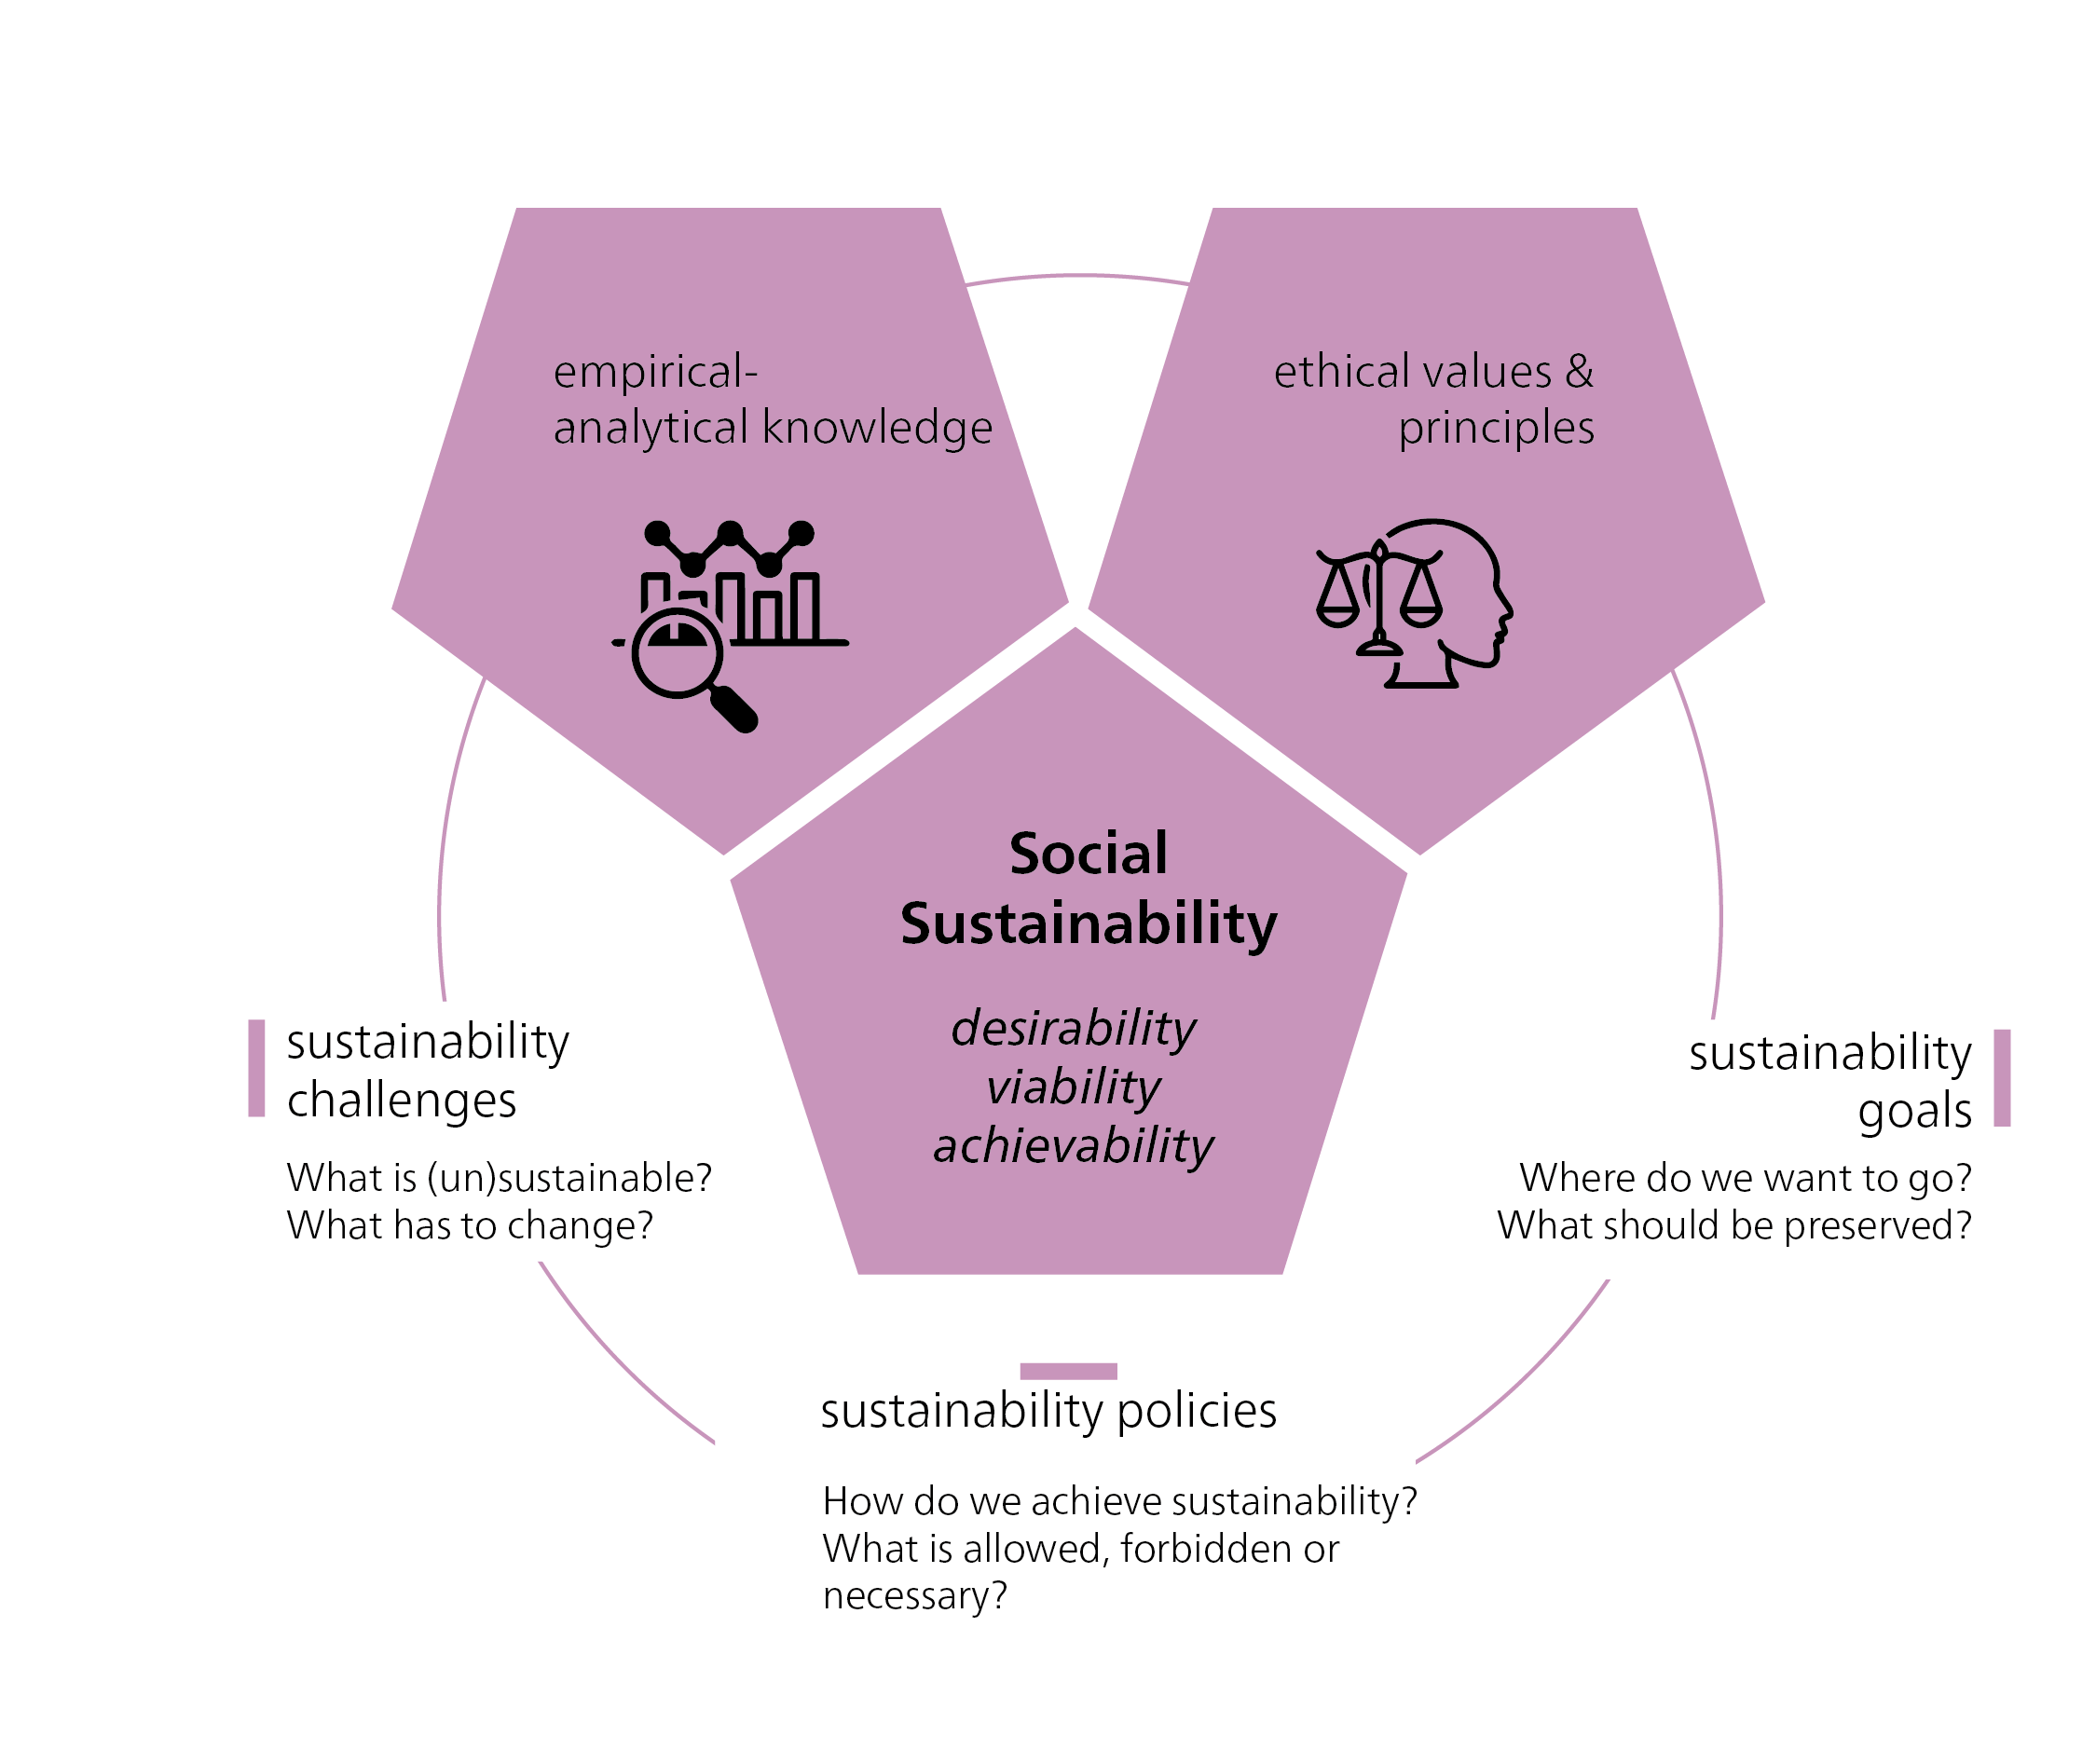
\includegraphics[keepaspectratio]{4_social-sustainability/images/Fig4_1_NESocial.png}}

}

\caption{\label{fig-NESocial}Soziale Nachhaltigkeit. Quelle: Eigene
Darstellung}

\end{figure}%

Diese Aspekte werden durch Kate Raworths Donut-Ökonomik (2017a)
veranschaulicht, einem Rahmen, der die SDGs und Menschenrechte als
Grundlage für sozial nachhaltige und gerechte menschliche Aktivitäten
betrachtet. In der Donut-Ökonomik ist die Befriedigung der
Grundbedürfnisse aller Menschen zentral. Diese Grundbedürfnisse, die das
soziale Fundament des Rahmens bilden, umfassen Zugang zu sauberem
Wasser, Sanitärversorgung, Gesundheitsversorgung, Bildung, Nahrung,
sauberen Kochgelegenheiten, Strom, Wohnraum sowie Informations- und
Unterstützungsnetzwerken, sowie die Möglichkeit zu arbeiten und ein
Einkommen zu erzielen. Weitere Faktoren, die das soziale Fundament
bilden, sind Geschlechtergleichstellung, soziale Gleichheit, Frieden und
Gerechtigkeit sowie politische Teilhabe -- d.~h. die Möglichkeit,
gesellschaftlichen Einfluss auszuüben.

In der Donut-Ökonomik könnten Wirtschaftspolitiken dazu beitragen,
soziale Gerechtigkeit zu erreichen, indem Vorteile und Kosten verteilt
werden, ohne planetare Grenzen zu überschreiten. Und darin liegt die
Herausforderung: Länder, die hinsichtlich sozialer
Nachhaltigkeitsindikatoren -- z. B. Zugang zu Nahrung, Bildung oder
Wohnraum -- gut abschneiden, überschreiten häufig ökologische Grenzen.
Umgekehrt schneiden Länder, die innerhalb dieser ökologischen Grenzen
bleiben, oft in sozialen Bereichen schlecht ab
vgl.~\ref{fig-SocEcoBoundaries}. Ein Gleichgewicht zwischen sozialen und
ökologischen Anforderungen herzustellen ist daher entscheidend.

\begin{figure}[H]

\centering{

\pandocbounded{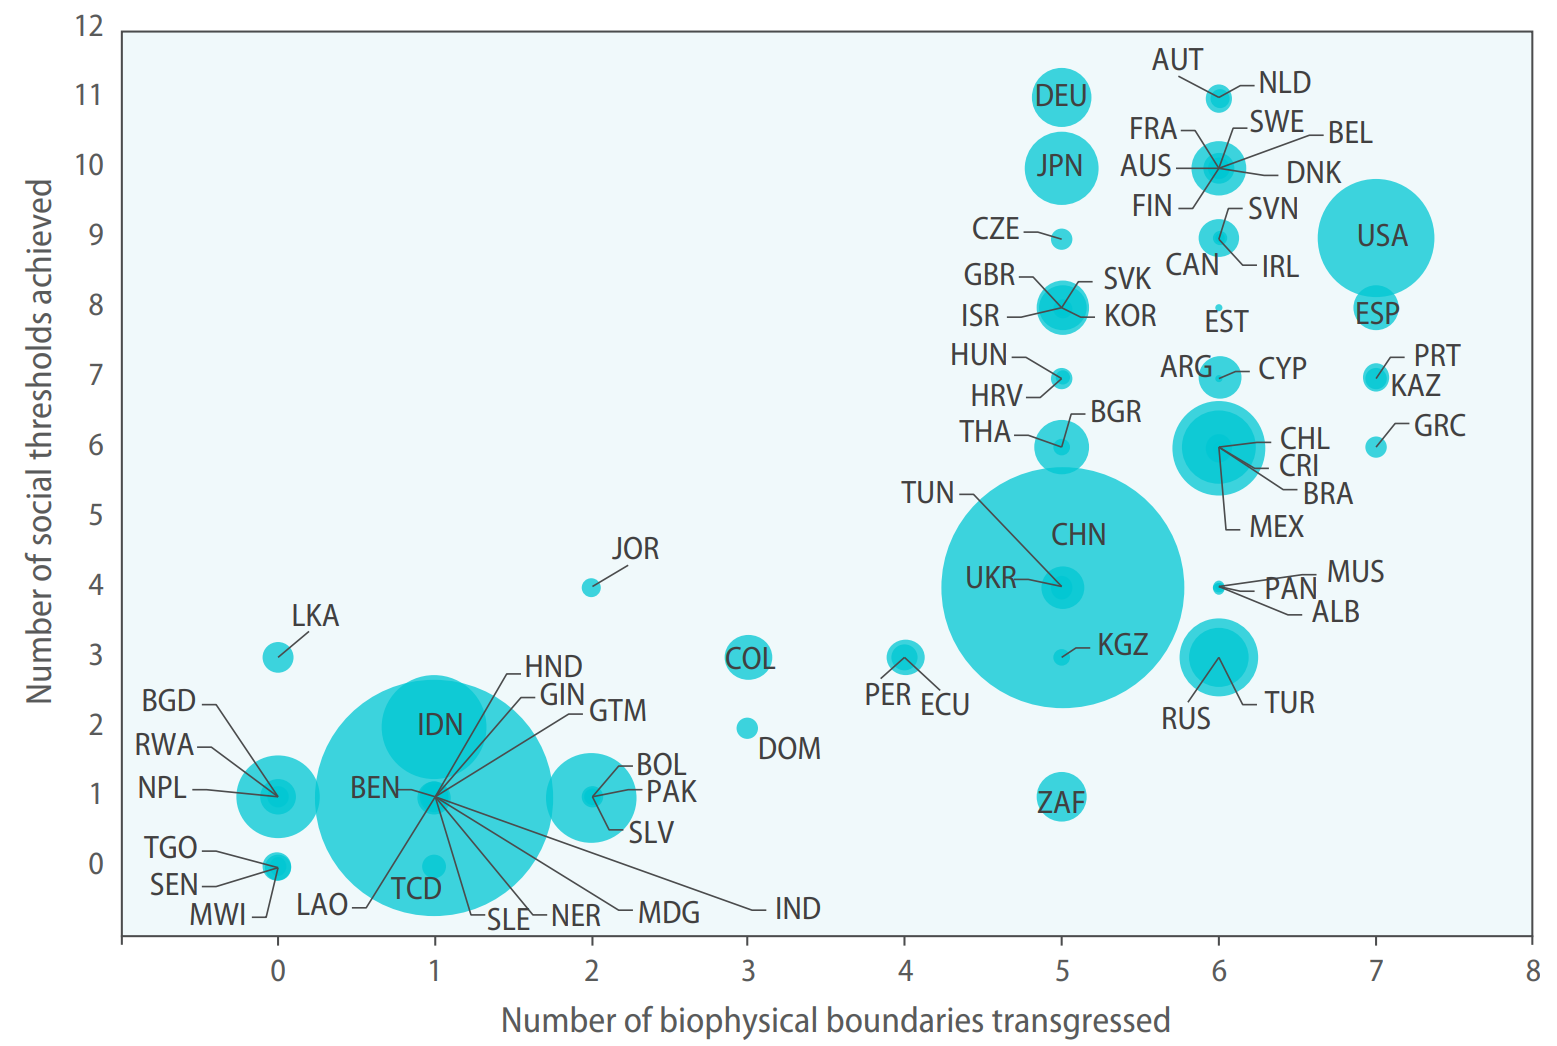
\includegraphics[keepaspectratio]{4_social-sustainability/images/Fig4_2_SocialEcologicalBoundaries.png}}

}

\caption{\label{fig-SocEcoBoundaries}Erreichte soziale Schwellenwerte
gegenüber überschrittenen biophysikalischen Grenzen für verschiedene
Länder, Ergebnisse gewichtet nach der jeweiligen Bevölkerungsgrösse.
Quelle: UN/DESA (2018) basierend auf O'Neill u.~a. (2018), Abbildung 2.}

\end{figure}%

Um eine nachhaltige Zukunft zu erreichen, argumentiert Raworth (2017a),
dass die Ressourcen der Erde gerechter verteilt werden müssen. Dies
würde es allen ermöglichen, ihre Grundbedürfnisse zu erfüllen und
gleichzeitig die Grenzen des Planeten zu respektieren. Es würde
Veränderungen im Lebensstil erfordern -- insbesondere bei den
Wohlhabenden, die für den Grossteil der Emissionen verantwortlich sind.
Derzeit tendieren diejenigen, die mehr Emissionen verursachen, zu einem
besseren Zugang zu wesentlichen Gütern wie Nahrung, Wasser, Energie und
Bildung -- genau jenen Dingen, an denen es Menschen in
einkommensschwächeren Ländern oft mangelt. In wohlhabenderen Ländern
werden die Grundbedürfnisse der Menschen in der Regel umfassender
erfüllt, was zu mehr Wohlstand, Gleichheit und Gerechtigkeit führt.
Gleichzeitig sind höhere Lebensstandards oft mit erhöhten
Treibhausgasemissionen und erhöhtem Konsum verbunden -- wie in
westlichen Industrieländern (z. B. USA, Europa) und China zu beobachten.

Ein weiterer Ansatz zur sozialen Nachhaltigkeit findet sich in den Human
Development Reports der Vereinten Nationen, die ein auf dem
Fähigkeitenansatz basierendes Modell menschlicher Entwicklung verwenden
vgl.~\ref{sec-CA}. Der Fähigkeitenansatz fragt, was eine Person braucht,
um ein gutes und erfülltes Leben zu führen. Da verschiedene Menschen
unterschiedliche Ressourcen benötigen, um dies zu erreichen, fördert das
Geben desselben für alle keine echte Gleichheit. Stattdessen sollten wir
jeder Person das geben, was sie braucht, um ein Leben zu führen, das sie
wertschätzen kann. Dieses Modell menschlicher Entwicklung fördert die
Achtung der Menschenwürde als unveräusserliches Recht und befürwortet
die Bereitstellung realistischer Möglichkeiten für alle, aufzublühen.

\subsection{Dimensionen der Gerechtigkeit}\label{sec-Dimjustice}

Donut-Ökonomik und Fähigkeitenansatz sind zwei Beispiele für prägnante
und einflussreiche normative Rahmenwerke. In diesem Kapitel behandeln
wir eine Reihe von Konzepten und Ansätzen, die -- durch ihre sozialen
Dimensionen -- inhärent normative und ethische Überlegungen beinhalten.

Die vielen Theorien und Konzepte sozialer Nachhaltigkeit sind auch mit
unterschiedlichen Vorstellungen von „Gerechtigkeit'' verknüpft. Einige
davon werden in Kapitel~\ref{sec-justice} näher beschrieben. Drei häufig
genannte Dimensionen sind: Verteilungsgerechtigkeit,
Verfahrensgerechtigkeit und Anerkennungsgerechtigkeit ({de Bruin u.~a.}
2024; Tribaldos und Kortetmäki 2022a; Wijsman und Berbés-Blázquez 2022).

\begin{figure}[H]

\centering{

\pandocbounded{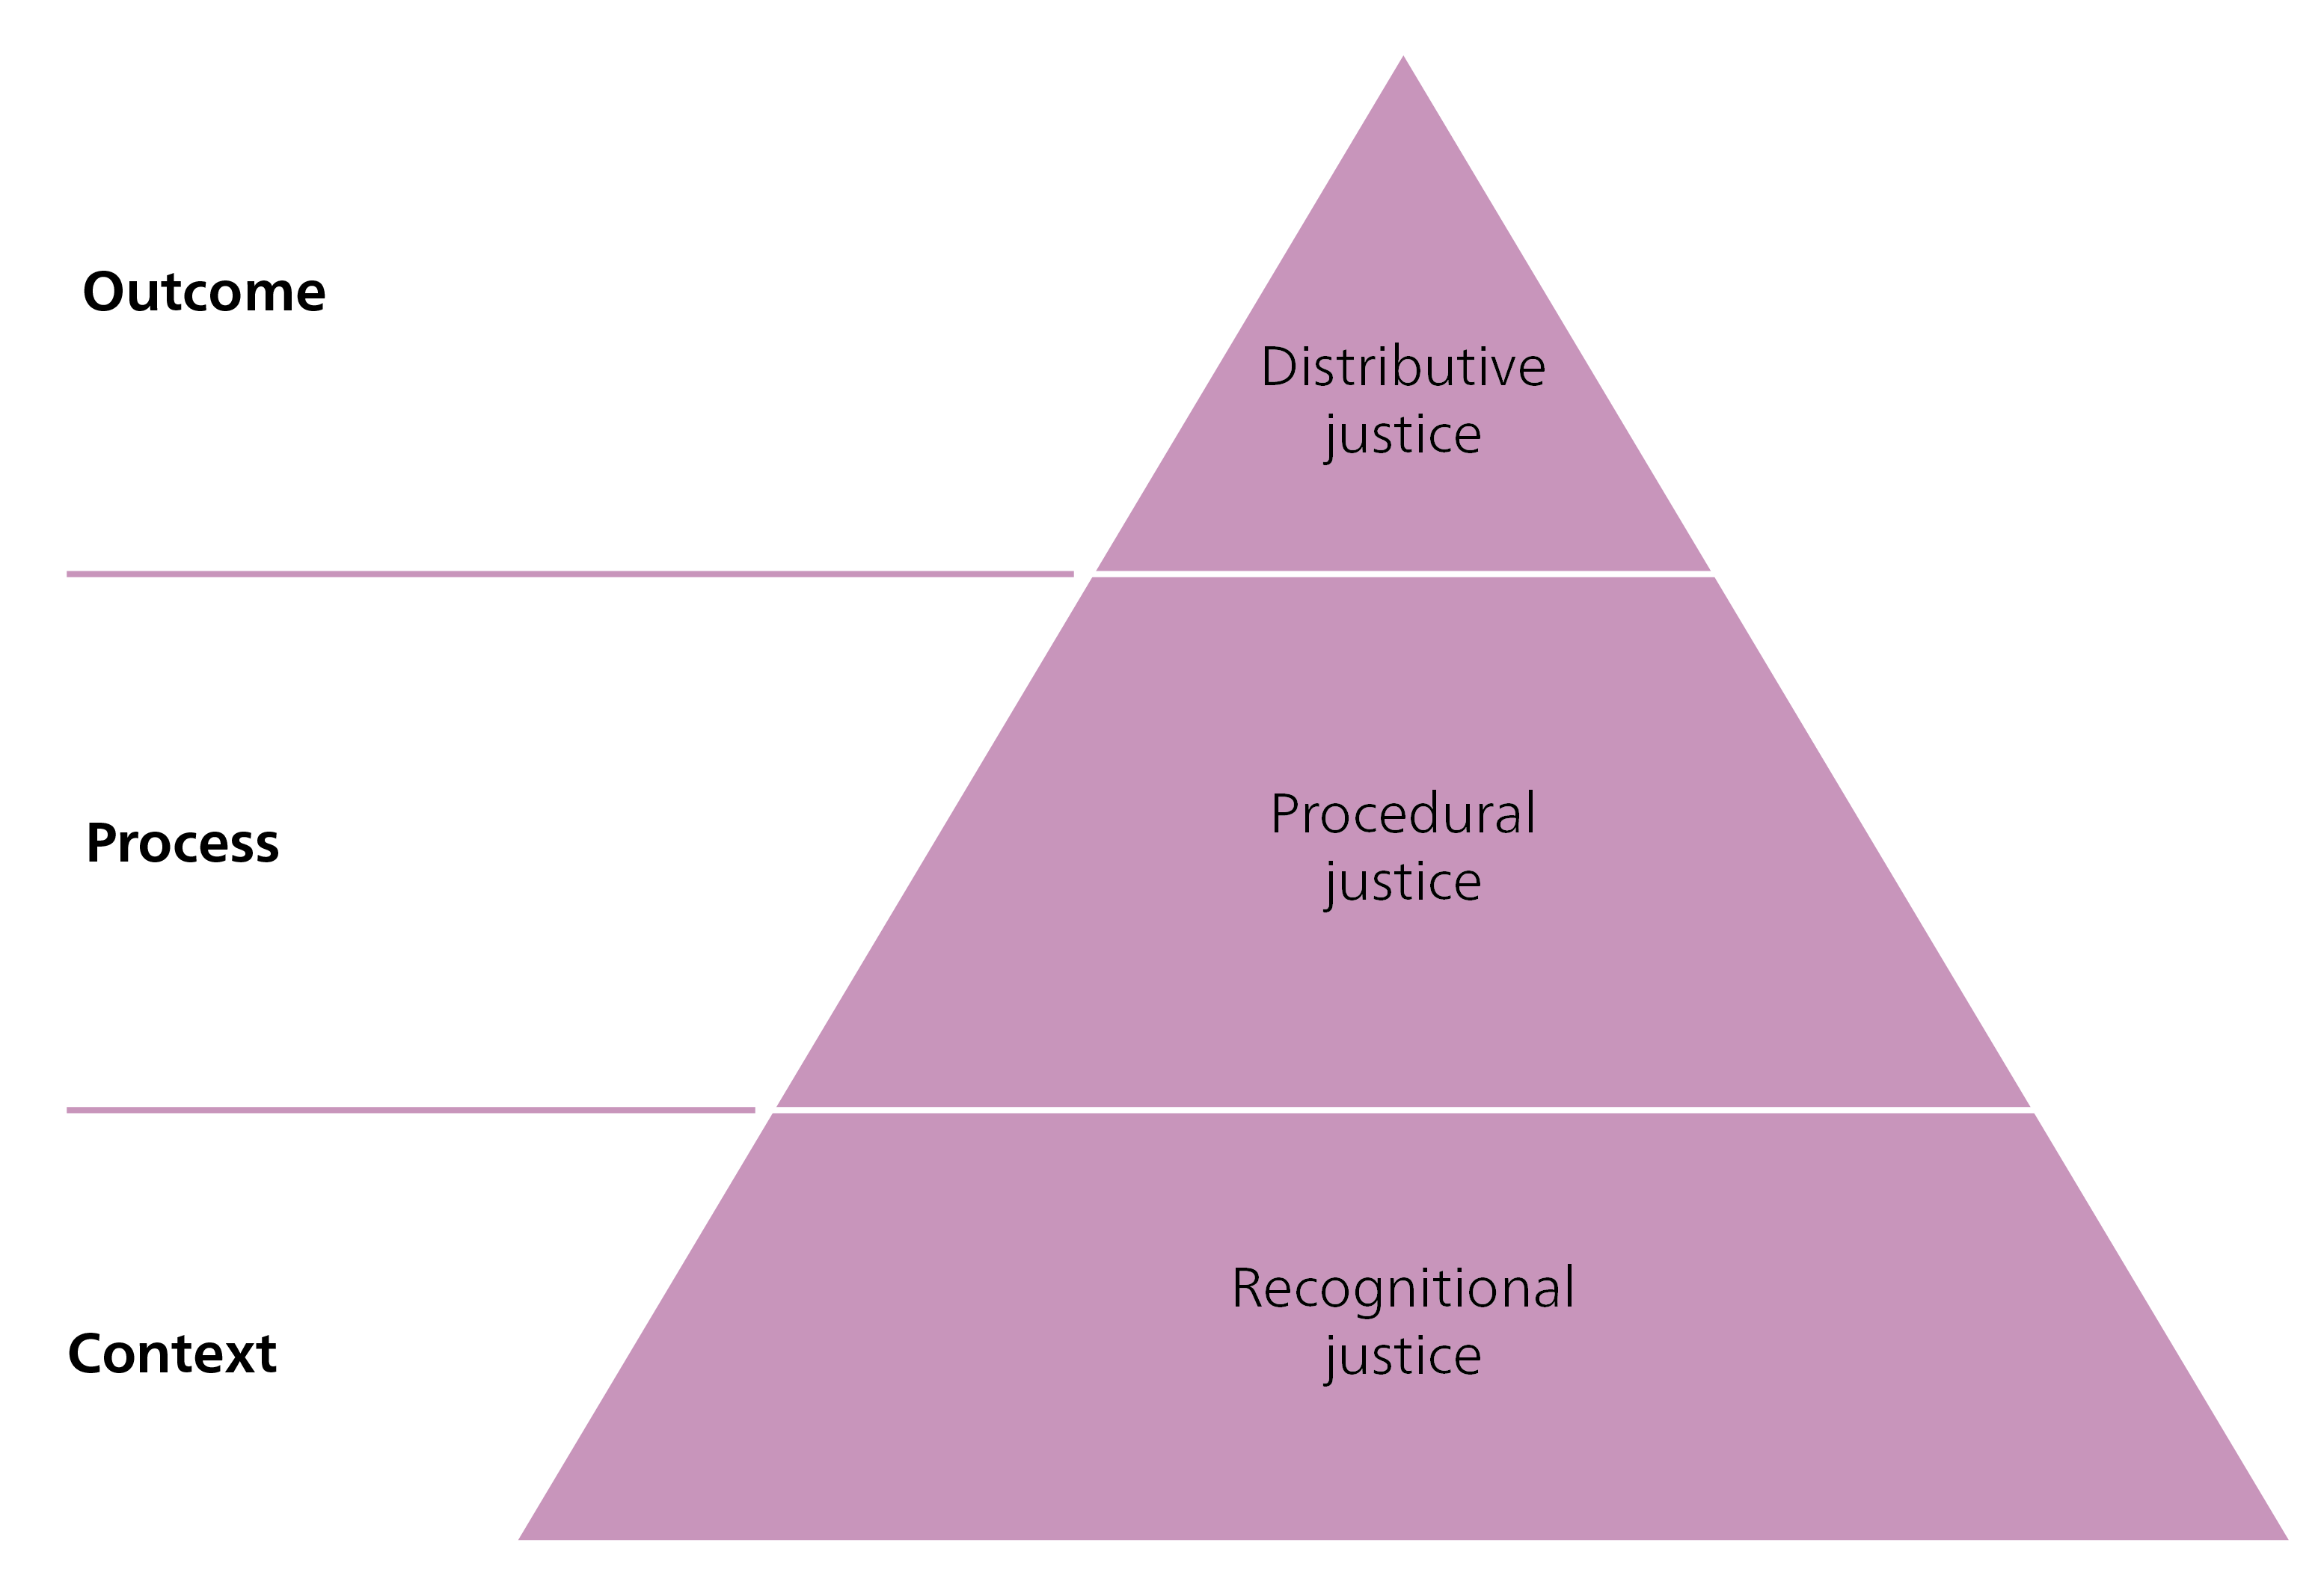
\includegraphics[keepaspectratio]{4_social-sustainability/images/Fig4_3_Justice.png}}

}

\caption{\label{fig-justice}Die jeweiligen Schwerpunktbereiche von
Verteilungsgerechtigkeit, Verfahrensgerechtigkeit und
Anerkennungsgerechtigkeit. Quelle: Eigene Darstellung, adaptiert nach
See und Wilmsen (2022).}

\end{figure}%

\textbf{Verteilungsgerechtigkeit} ist ein ergebnisorientiertes Konzept,
das auf eine faire Verteilung von Gütern und Lasten abzielt, unabhängig
von sozialen Unterschieden. Dieses Prinzip gilt für Fragen wie den
Zugang zu sauberem Wasser, die ungleiche Belastung durch
Umweltverschmutzung oder gleiche Bezahlung.

\textbf{Verfahrensgerechtigkeit} konzentriert sich auf die Inklusivität
von Entscheidungsprozessen. Sie fordert, dass unterrepräsentierte
Gruppen in Institutionen fair vertreten sind, sodass ihre Perspektiven
in Entscheidungsprozesse eingehört und einbezogen werden können.

\textbf{Anerkennungsgerechtigkeit} betont die Bedeutung des Kontexts und
des Respekts vor sozialen und kulturellen Unterschieden. Sie beinhaltet
die Anerkennung struktureller Ungerechtigkeiten, den Respekt vor den
Würden und Werten verschiedener Menschen und sozialer Gruppen sowie das
Verständnis, dass unterschiedliche Bedürfnisse und Präferenzen in
verschiedenen historischen Erfahrungen, Identitäten und kulturellen
Hintergründen verwurzelt sind.

Tabelle~\ref{tbl-justice} zeigt, wie sich diese drei Dimensionen
gegenseitig beeinflussen (Wijsman und Berbés-Blázquez 2022). Eine
ausführlichere Diskussion von Verteilungs- und Verfahrensgerechtigkeit
folgt in Kapitel~\ref{sec-justice}, da dies die Dimensionen sind, die
Debatten über soziale Nachhaltigkeit am stärksten beeinflussen.

\begingroup\fontsize{8}{10}\selectfont

\begin{longtable}[t]{>{\raggedright\arraybackslash}p{1.6cm}>{\raggedright\arraybackslash}p{3.25cm}>{\raggedright\arraybackslash}p{3.25cm}>{\raggedright\arraybackslash}p{3.25cm}}

\caption{\label{tbl-justice}Zusammenhänge zwischen
Verteilungsgerechtigkeit, Verfahrensgerechtigkeit und
Anerkennungsgerechtigkeit. Quelle: Basierend auf Wijsman und
Berbés-Blázquez (2022).}

\tabularnewline

\toprule
\textbf{Dimension} & \textbf{Verteilungsgerechtigkeit} & \textbf{Verfahrensgerechtigkeit} & \textbf{Anerkennungsgerechtigkeit}\\
\midrule
\endfirsthead
\multicolumn{4}{@{}l}{\textit{(continued)}}\\
\toprule
\textbf{Dimension} & \textbf{Verteilungsgerechtigkeit} & \textbf{Verfahrensgerechtigkeit} & \textbf{Anerkennungsgerechtigkeit}\\
\midrule
\endhead

\endfoot
\bottomrule
\endlastfoot
\textbf{Verteilungs­gerechtigkeit} & — & Die Verteilung von Ressourcen kann beeinflussen, wie leicht oder schwer es für Einzelpersonen oder Gemeinschaften ist, an Entscheidungsprozessen teilzunehmen. Dies liegt daran, dass Teilhabe Zeit, Energie und finanzielle Ressourcen erfordert. & Die Verteilung von Ressourcen kann beeinflussen, wessen Interessen in Entscheidungsprozessen berücksichtigt werden – und wessen Identität anerkannt und als wichtig erachtet wird.\\
\textbf{Verfahrens­gerechtigkeit} & Die Teilnahme an Entscheidungsprozessen kann deren Ergebnisse beeinflussen – und damit, wie Vor- und Nachteile zwischen Einzelpersonen und Gruppen verteilt werden. & — & Die Teilnahme an Entscheidungsprozessen kann beeinflussen, wessen Interessen gehört werden und welche Einzelpersonen oder Gemeinschaften als wichtig anerkannt werden.\\
\textbf{Anerkennungs­gerechtigkeit} & Die Anerkennung von Einzelpersonen oder Gruppen als wertvoll kann beeinflussen, wie Ressourcen verteilt werden. & Die Anerkennung von Einzelpersonen oder Gruppen als wertvoll kann auch bestimmen, wer zur Teilnahme an Entscheidungsprozessen eingeladen wird. & —\\*

\end{longtable}

\endgroup{}

\section{Soziale Nachhaltigkeit
definieren}\label{soziale-nachhaltigkeit-definieren}

Im Laufe der Zeit haben sich Diskussionen über soziale Nachhaltigkeit
auf verschiedene Themen konzentriert. Dazu gehören Armutsbekämpfung,
Entwicklung, Grundbedürfnisse, Lebensgrundlagen und Gleichheit -- ebenso
wie Identität, Zugehörigkeit sowie Stabilität und Sicherheit von
Gemeinschaften (Glasson und Wood 2009). Diese thematische Vielfalt
spiegelt sich in den zahlreichen verfügbaren Definitionen sozialer
Nachhaltigkeit wider. Die Literatur wird in der Tat oft als
fragmentiert, vage oder bisweilen chaotisch beschrieben (Mehan und
Soflaei 2017). Einige Forscher*innen haben sogar argumentiert, dass sich
das Konzept der sozialen Nachhaltigkeit in den letzten 30 Jahren stärker
verändert hat als die ökologischen und wirtschaftlichen Dimensionen
(Foladori 2005).

Soziale Nachhaltigkeit lässt sich daher am besten als ein dynamisches
Konzept verstehen, das je nach Zeit und Ort unterschiedliche Formen
annimmt (Boyer u.~a. 2016; Dempsey u.~a. 2011). Soziale Prioritäten sind
vielfältig und kontextspezifisch und verändern sich im Laufe der Zeit.
Zudem gibt es erhebliche kulturelle und lokale Unterschiede hinsichtlich
dessen, was als sozial vertretbar und wünschenswert gilt.

Trotz dieser Vielfalt beschreiben Definitionen sozialer Nachhaltigkeit
im Allgemeinen einen positiven Zustand, der bereits besteht oder als
erreichbar gilt. Er wird häufig mit dem Ziel verbunden, den sozialen
Zusammenhalt zu stärken und grundlegende Dienstleistungen
bereitzustellen, die zum Wohlergehen beitragen, wie
Gesundheitsversorgung, Bildung, Mobilität, Wohnraum oder
Freizeitangebote. Soziale Nachhaltigkeit ist dann erreicht, wenn soziale
Prozesse, Systeme, Strukturen und Beziehungen aktiv dazu beitragen, dass
aktuelle und künftige Generationen gesunde und lebensfähige
Gemeinschaften aufbauen können.

Für die Brundtland-Kommission (1987b) besteht das Hauptziel der sozialen
Dimension nachhaltiger Entwicklung darin, grundlegende menschliche
Bedürfnisse zu erfüllen. Diese umfassen nicht nur sauberes Wasser,
Nahrung und Sicherheit -- sie erstrecken sich auch auf Aspekte wie
Wohlergehen, Gerechtigkeit, ein demokratisches Regierungssystem und eine
lebendige Zivilgesellschaft. Diese umfassende Definition kann in
verschiedenen Kontexten flexibel angewendet werden.

Um einen konkreteren Rahmen bereitzustellen, schlagen Barron u.~a.
(2023) und Cuesta u.~a. (2024) folgenden strukturierten Ansatz vor (vgl.
Abbildung~\ref{fig-framework}).

\begin{figure}[H]

\centering{

\pandocbounded{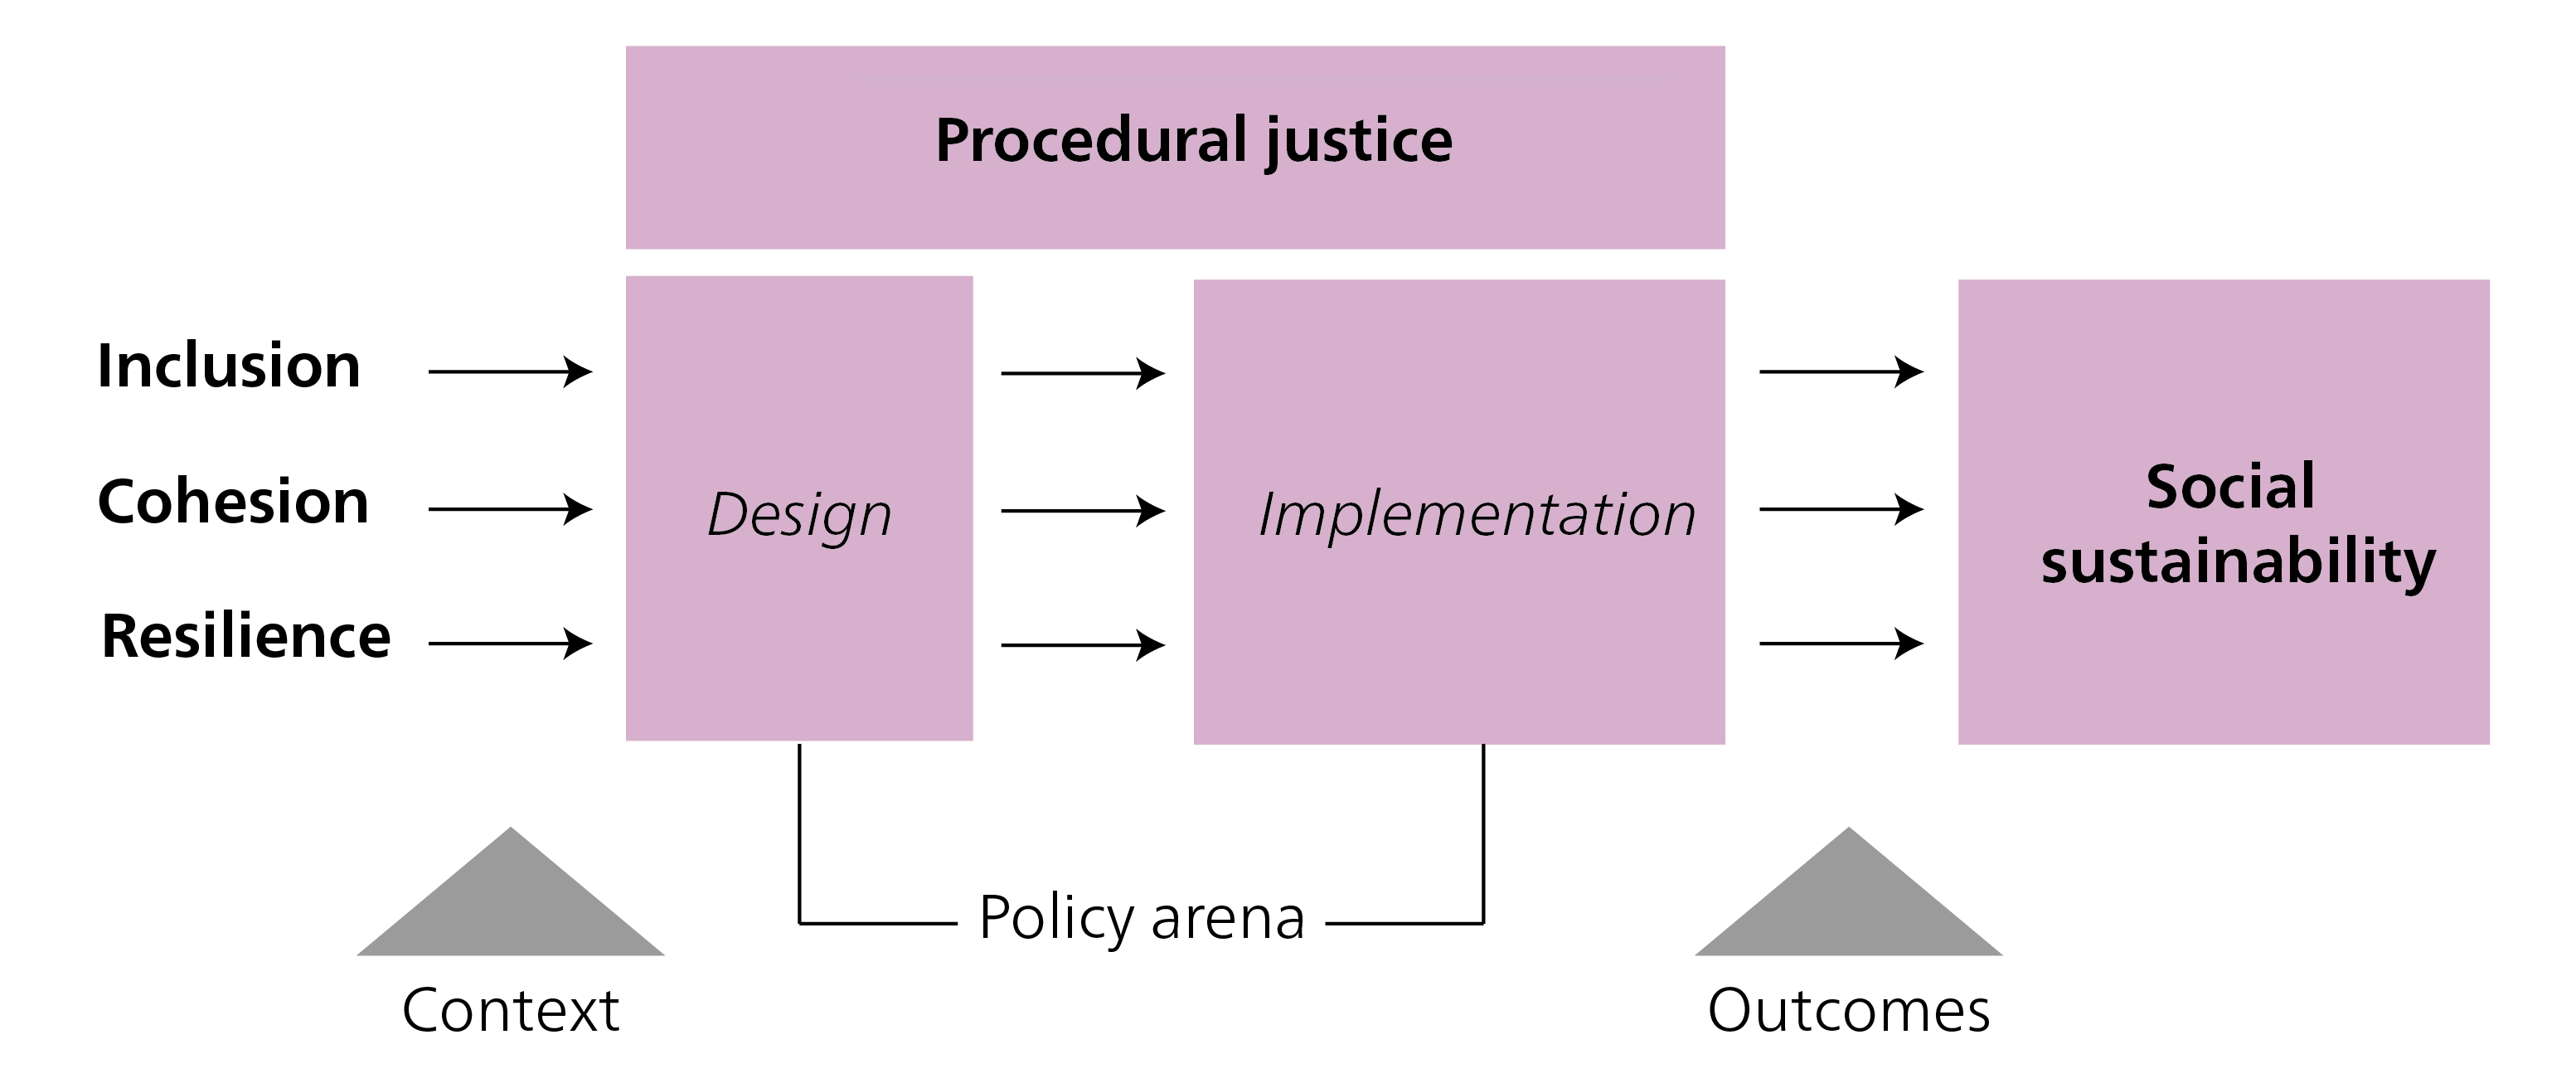
\includegraphics[keepaspectratio]{4_social-sustainability/images/Fig4_4_Framework.png}}

}

\caption{\label{fig-framework}Ein strukturierter Ansatz zur sozialen
Nachhaltigkeit. Adaptiert nach Barron et al.~(2023, S. 31) \& Cuesta et
al.~(2024).}

\end{figure}%

Die linke Seite von Abbildung Abbildung~\ref{fig-framework} zeigt drei
Dimensionen eines bestimmten Kontexts, nämlich: Inklusion, sozialer
Zusammenhalt und Resilienz. Jede dieser Dimensionen -- im Folgenden
definiert -- kann in einer Gemeinschaft oder Gesellschaft in
unterschiedlichem Ausmass vorhanden sein:

\begin{enumerate}
\def\labelenumi{\arabic{enumi}.}
\item
  \textbf{Inklusion} bezeichnet den Zugang aller Einzelpersonen und
  Gruppen zu den wirtschaftlichen, politischen, sozialen und kulturellen
  Sphären.
\item
  \textbf{Sozialer Zusammenhalt} ist ein gemeinsames Zugehörigkeits- und
  Vertrauensgefühl, das Gemeinschaften und Gruppen ermöglicht, ohne
  Konflikte zusammenzuarbeiten.
\item
  \textbf{Resilienz} bezeichnet die Fähigkeit, interne oder externe
  Schocks -- wie Umweltveränderungen oder politische Krisen -- zu
  vermeiden oder deren Auswirkungen abzufedern.
\end{enumerate}

Der mittlere Teil betont die Bedeutung von
\textbf{Verfahrensgerechtigkeit} -- der Fairness von
Entscheidungsprozessen bei der \textbf{Gestaltung} und
\textbf{Umsetzung} von Politiken und Programmen. Wenn diese Prozesse als
fair, transparent und vertrauenswürdig wahrgenommen werden, erzeugen sie
\textbf{Prozesslegitimität}, d.~h. die Menschen akzeptieren die
Autorität von Entscheidungen und sind eher bereit, diese zu unterstützen
und zu befolgen. Der Prozess der Gestaltung und Umsetzung von Politiken
und Programmen findet in einer sogenannten „policy arena''
(Politikarena) statt. Der Begriff „Politikarena'' ist weit gefasst und
umfasst politische Foren auf lokaler, nationaler, regionaler oder
globaler Ebene, in denen Ressourcen zugeteilt, Ziele gesetzt und
Entscheidungen getroffen werden.

Schliesslich zeigt die rechte Seite der Abbildung die Ergebnisse des
Gestaltungs- und Umsetzungsprozesses. Dieser Prozess kann Inklusion,
sozialen Zusammenhalt und Resilienz fördern -- aber auch hemmen. Diese
Ergebnisse beeinflussen wiederum das künftige Niveau sozialer
Nachhaltigkeit. Mit anderen Worten: Soziale Nachhaltigkeit ist dann
gegeben, wenn Inklusion, sozialer Zusammenhalt und Resilienz im Laufe
der Zeit schrittweise gestärkt werden -- idealerweise in einem legitimen
und transparenten Prozess.

Die folgenden Abschnitte erläutern die Kernelemente Inklusion, sozialer
Zusammenhalt, Resilienz und Gerechtigkeit (sowohl Verfahrens- als auch
Verteilungsgerechtigkeit) näher.

\section{Inklusion}\label{inklusion}

Inklusion befasst sich mit Fragen sozialer Ungleichheit. Soziale
Inklusion zielt darauf ab, allen Menschen die Teilhabe an der
Gesellschaft zu ermöglichen -- insbesondere durch den Abbau tief
verwurzelter systemischer Benachteiligungen. Viele Einzelpersonen und
Gruppen stehen vor Barrieren, die ihre sozioökonomische Teilhabe
einschränken. Solche Barrieren können Armut oder ein geringes Einkommen
umfassen; andere Formen von Diskriminierung und Ausgrenzung können auf
Geschlecht, Alter, Herkunft, Beruf, Ethnizität, Religion, Nationalität,
Behinderung, sexueller Orientierung oder Geschlechtsidentität basieren.
Solche Ungleichheiten werden durch formelle und informelle Normen,
Verhaltensweisen, Gesetze und Institutionen verstärkt.

Dies wirft normative Fragen auf: Ab wann gilt Ungleichheit als
problematisch? Und welches Mass an Ungleichheit ist sozial inakzeptabel?
Inklusion sollte nicht als eine Form der Wohltätigkeit verstanden
werden, d.~h. als etwas, das nur aus ethischen Gründen „richtig'' ist.
Die Verringerung von Ungleichheiten hat erhebliche Vorteile für die
gesamte Gesellschaft. Grössere Inklusion und Chancengleichheit führen zu
besseren Ergebnissen in Bezug auf Einkommen, Armutsbekämpfung und
Humankapital (OECD 2015).

Eine US-amerikanische Studie von Hsieh u.~a. (2013) fand beispielsweise
heraus, dass eine Verringerung der Diskriminierung gegenüber weiblichen
und schwarzen Arbeitnehmer*innen zwischen 1960 und 2010 für 15 bis 20\%
des Wirtschaftswachstums pro Arbeitnehmer*in verantwortlich war. Dieses
Wachstum wurde auf eine Zunahme talentierter Menschen zurückgeführt, die
Zugang zu besseren Möglichkeiten erhielten. Andere Studien zeigen, dass
Geschlechterungleichheit negative Auswirkungen auf das
Wirtschaftswachstum haben kann (Fabrizio u.~a. (2018); Klasen und
Lamanna (2009)). Es gibt auch einen Zusammenhang zwischen Inklusion und
sozialer Stabilität: Länder, die aktiv die politische Teilhabe und
Inklusion benachteiligter Gruppen fördern, erfahren tendenziell weniger
soziale Konflikte (United Nations und World Bank 2018).

Kurz gesagt: Die Kosten sozialer Ungleichheit -- wie weniger
Bildungsmöglichkeiten, niedrigere Lebenseinkommen oder schlechtere
Gesundheit (Buehren u.~a. 2019; {Wodon und de la Briere} 2018) -- sind
nicht nur ethische Fragen. Sie beeinflussen auch die Gesamtwirtschaft,
da sie Potenziale reduzieren, die Produktivität schwächen und das
Konfliktrisiko erhöhen. Im Gegensatz dazu sind inklusivere
Gesellschaften gerechter, stabiler und wirtschaftlich effizienter.

\subsection{(Un-)Gleichheit}\label{sec-CA}

Da Ungleichheit komplex und vielschichtig ist, gibt es verschiedene
Möglichkeiten, sie zu analysieren, zu messen und zu bewerten. Dabei geht
es darum, Fragen zu stellen, \emph{wer} betroffen ist und \emph{wo} --
und in \emph{welchen} Bereichen Ungleichheiten auftreten
vgl.~\ref{fig-EqualityWhat}.

\begin{figure}[H]

\centering{

\pandocbounded{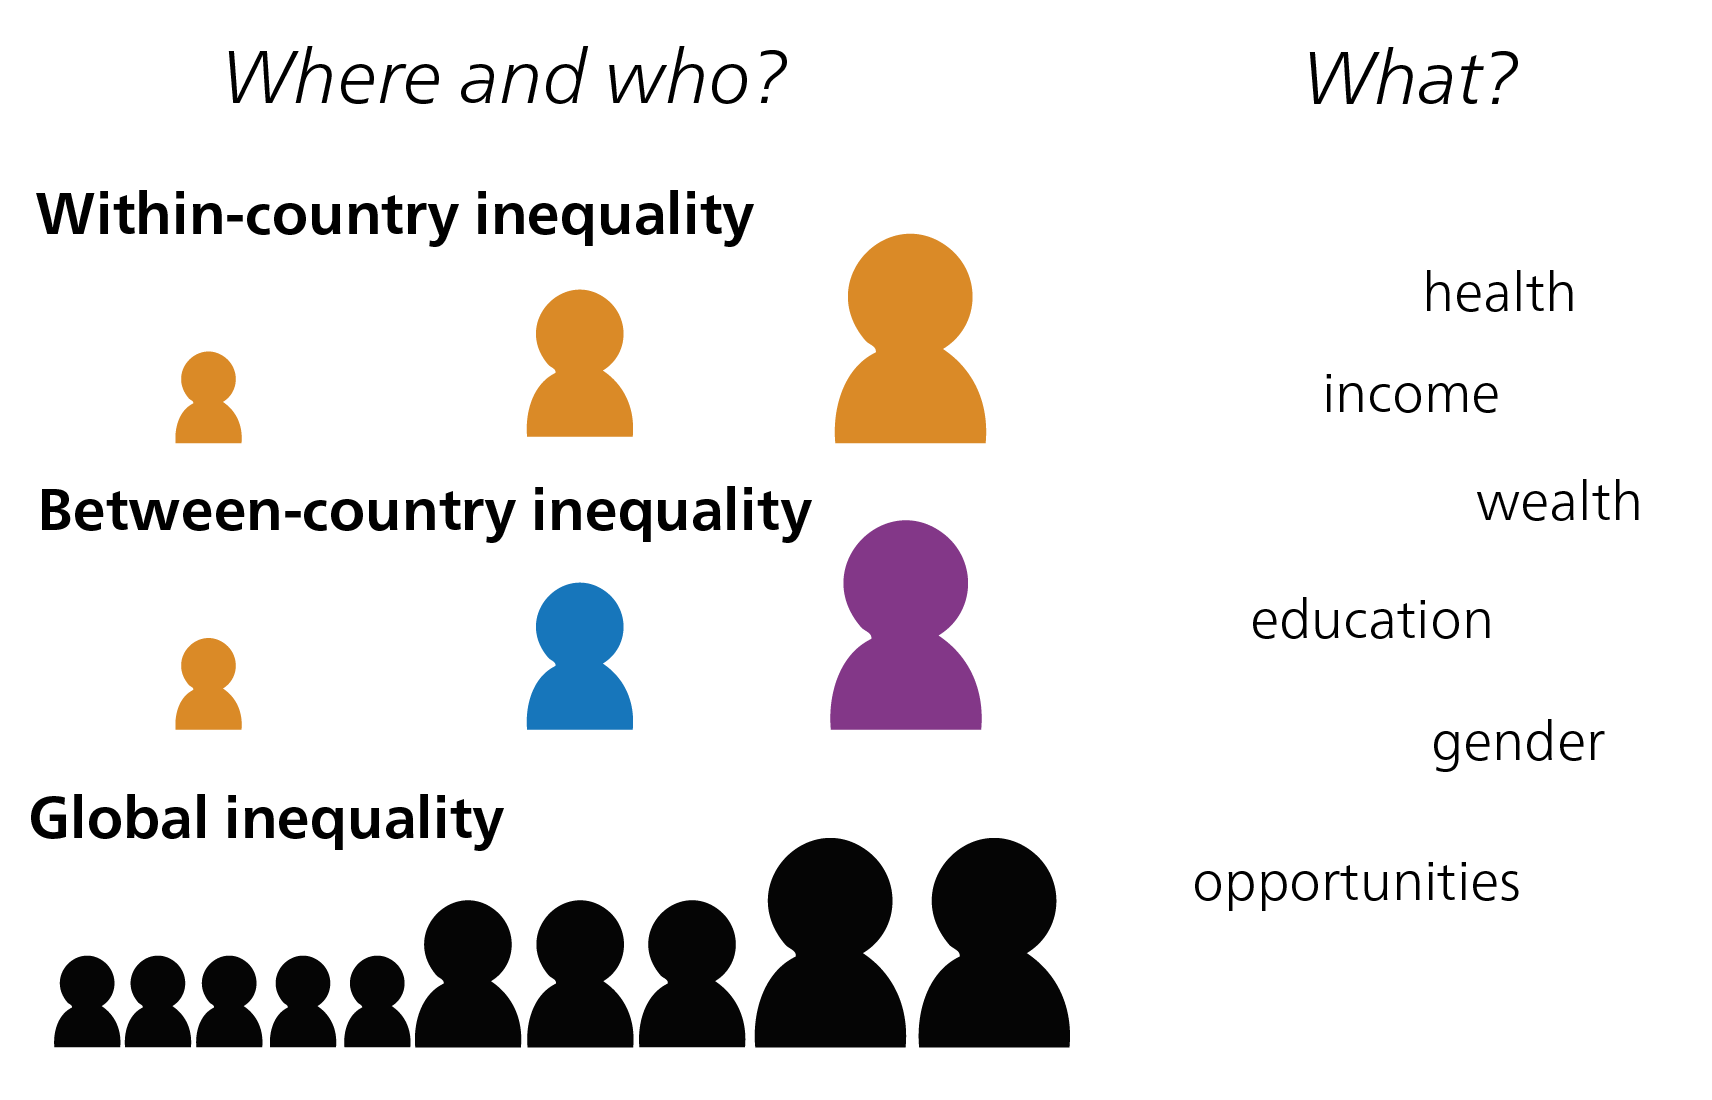
\includegraphics[keepaspectratio]{4_social-sustainability/images/Fig4_5_EqualityWhat.png}}

}

\caption{\label{fig-EqualityWhat}Gleichheit wofür? Quelle: Eigene
Darstellung, basierend auf Sen (1979)}

\end{figure}%

Ungleichheit kann aus verschiedenen Perspektiven betrachtet werden. Im
Folgenden gehen wir näher auf den bereits erwähnten Fähigkeitenansatz
ein.

\textbf{Ungleichheit betrachten: Geleitet von Sens Frage „Gleichheit
wofür?'' -- der Fähigkeitenansatz}

Der \textbf{Fähigkeitenansatz} bietet einen normativen Rahmen zur
Bewertung von Ungleichheit und menschlichem Wohlergehen, der über
herkömmliche Verteilungsprinzipien hinausgeht. Traditionelle Ansätze der
Verteilungsgerechtigkeit zielen entweder auf eine gleiche Verteilung
nach Leistung oder auf die Garantie eines Mindestmasses an Ressourcen
für alle ab. Eine vollständige Gleichheit zwischen Individuen -- d.~h.
\emph{Ergebnisgleichheit} -- ist jedoch nahezu unmöglich zu erreichen,
da viele Einflussfaktoren zufällig oder ungerecht verteilt sind. Es gilt
daher als fairer, sich auf \emph{Chancengleichheit} zu konzentrieren.
Dieses Prinzip zielt darauf ab, jeder Person die Möglichkeit zu geben,
ein bedeutsames und würdiges Leben mit Zugang zu zumindest einem
Mindestmass an Wohlstand zu führen. Dieses Minimum sollte ausreichen, um
Grundbedürfnisse zu decken und gleiche Bürgerrechte zu garantieren,
sodass alle das haben, was sie zur Befriedigung ihrer Bedürfnisse und
zur gleichberechtigten Teilhabe an der Gesellschaft brauchen.

Der in den 1980er Jahren vom indischen Ökonomen, Philosophen und
Nobelpreisträger \textbf{Amartya Sen} entwickelte und später von der
Philosophin \textbf{Martha Nussbaum} erweiterte Fähigkeitenansatz dient
als Alternative zur traditionellen Wohlfahrtsökonomie, die Wohlstand
primär anhand wirtschaftlicher Indikatoren misst (Roder 2020). Der
Fähigkeitenansatz lenkt die Aufmerksamkeit weg von formellen Ansprüchen
oder wirtschaftlichen Aggregaten hin zu den \textbf{realen Freiheiten
der Menschen, das Leben zu führen, das sie schätzen}. Er betont, dass
echte Entwicklung nicht nur vom Vorhandensein von Möglichkeiten und
Ressourcen abhängt, sondern auch davon, ob Einzelpersonen diese in der
Praxis tatsächlich nutzen können. Dies wiederum wird durch persönliche
Faktoren wie Gesundheit oder Behinderung sowie durch soziale, politische
und umweltbezogene Bedingungen geprägt. Für Menschen mit Behinderungen
beispielsweise erfordert Wohlergehen mehr als die formelle Anerkennung
von Rechten; es hängt von einer inklusiven Gesellschaft ab, die
Barrieren abbaut, Diskriminierung bekämpft, Zugang zu Bildung
sicherstellt und die Teilhabe an politischen und gesellschaftlichen
Entscheidungsprozessen ermöglicht.

Der Fähigkeitenansatz definiert Wohlergehen in Bezug auf
\textbf{Befähigungen} und \textbf{Funktionsweisen}. Befähigungen sind
reale Handlungsmöglichkeiten -- d.~h. was Menschen tun oder sein
könnten, wenn sie frei wählen könnten. Zum Beispiel gut ernährt zu sein,
zu heiraten, gebildet zu sein oder ohne Einschränkungen zu reisen.
Funktionsweisen sind die Befähigungen, die tatsächlich verwirklicht
werden. Ob Menschen verfügbare Ressourcen wie Einkommen, Bildung oder
öffentliche Dienstleistungen in Funktionsweisen umwandeln können, hängt
von \textbf{Umwandlungsfaktoren} ab. Dazu gehören persönliche Merkmale,
soziale Strukturen und Umweltbedingungen. Sie bestimmen letztlich, ob
Befähigungen und Funktionsweisen tatsächlich genutzt werden können.

Der Fähigkeitenansatz verlagert den Fokus daher von \textbf{Gleichheit}
zu \textbf{Gerechtigkeit/Fairness}. Während \emph{Gleichheit} darauf
abzielt, dass alle die gleichen Ressourcen erhalten (d.~h. Input),
konzentriert sich \emph{Gerechtigkeit/Fairness} auf das Ergebnis: Was
braucht eine Person, um ein vergleichbares Wohlergehen zu erreichen
(d.~h. Output)? (vgl. Abbildung~\ref{fig-EqualityEquity}).

\begin{figure}[H]

\centering{

\pandocbounded{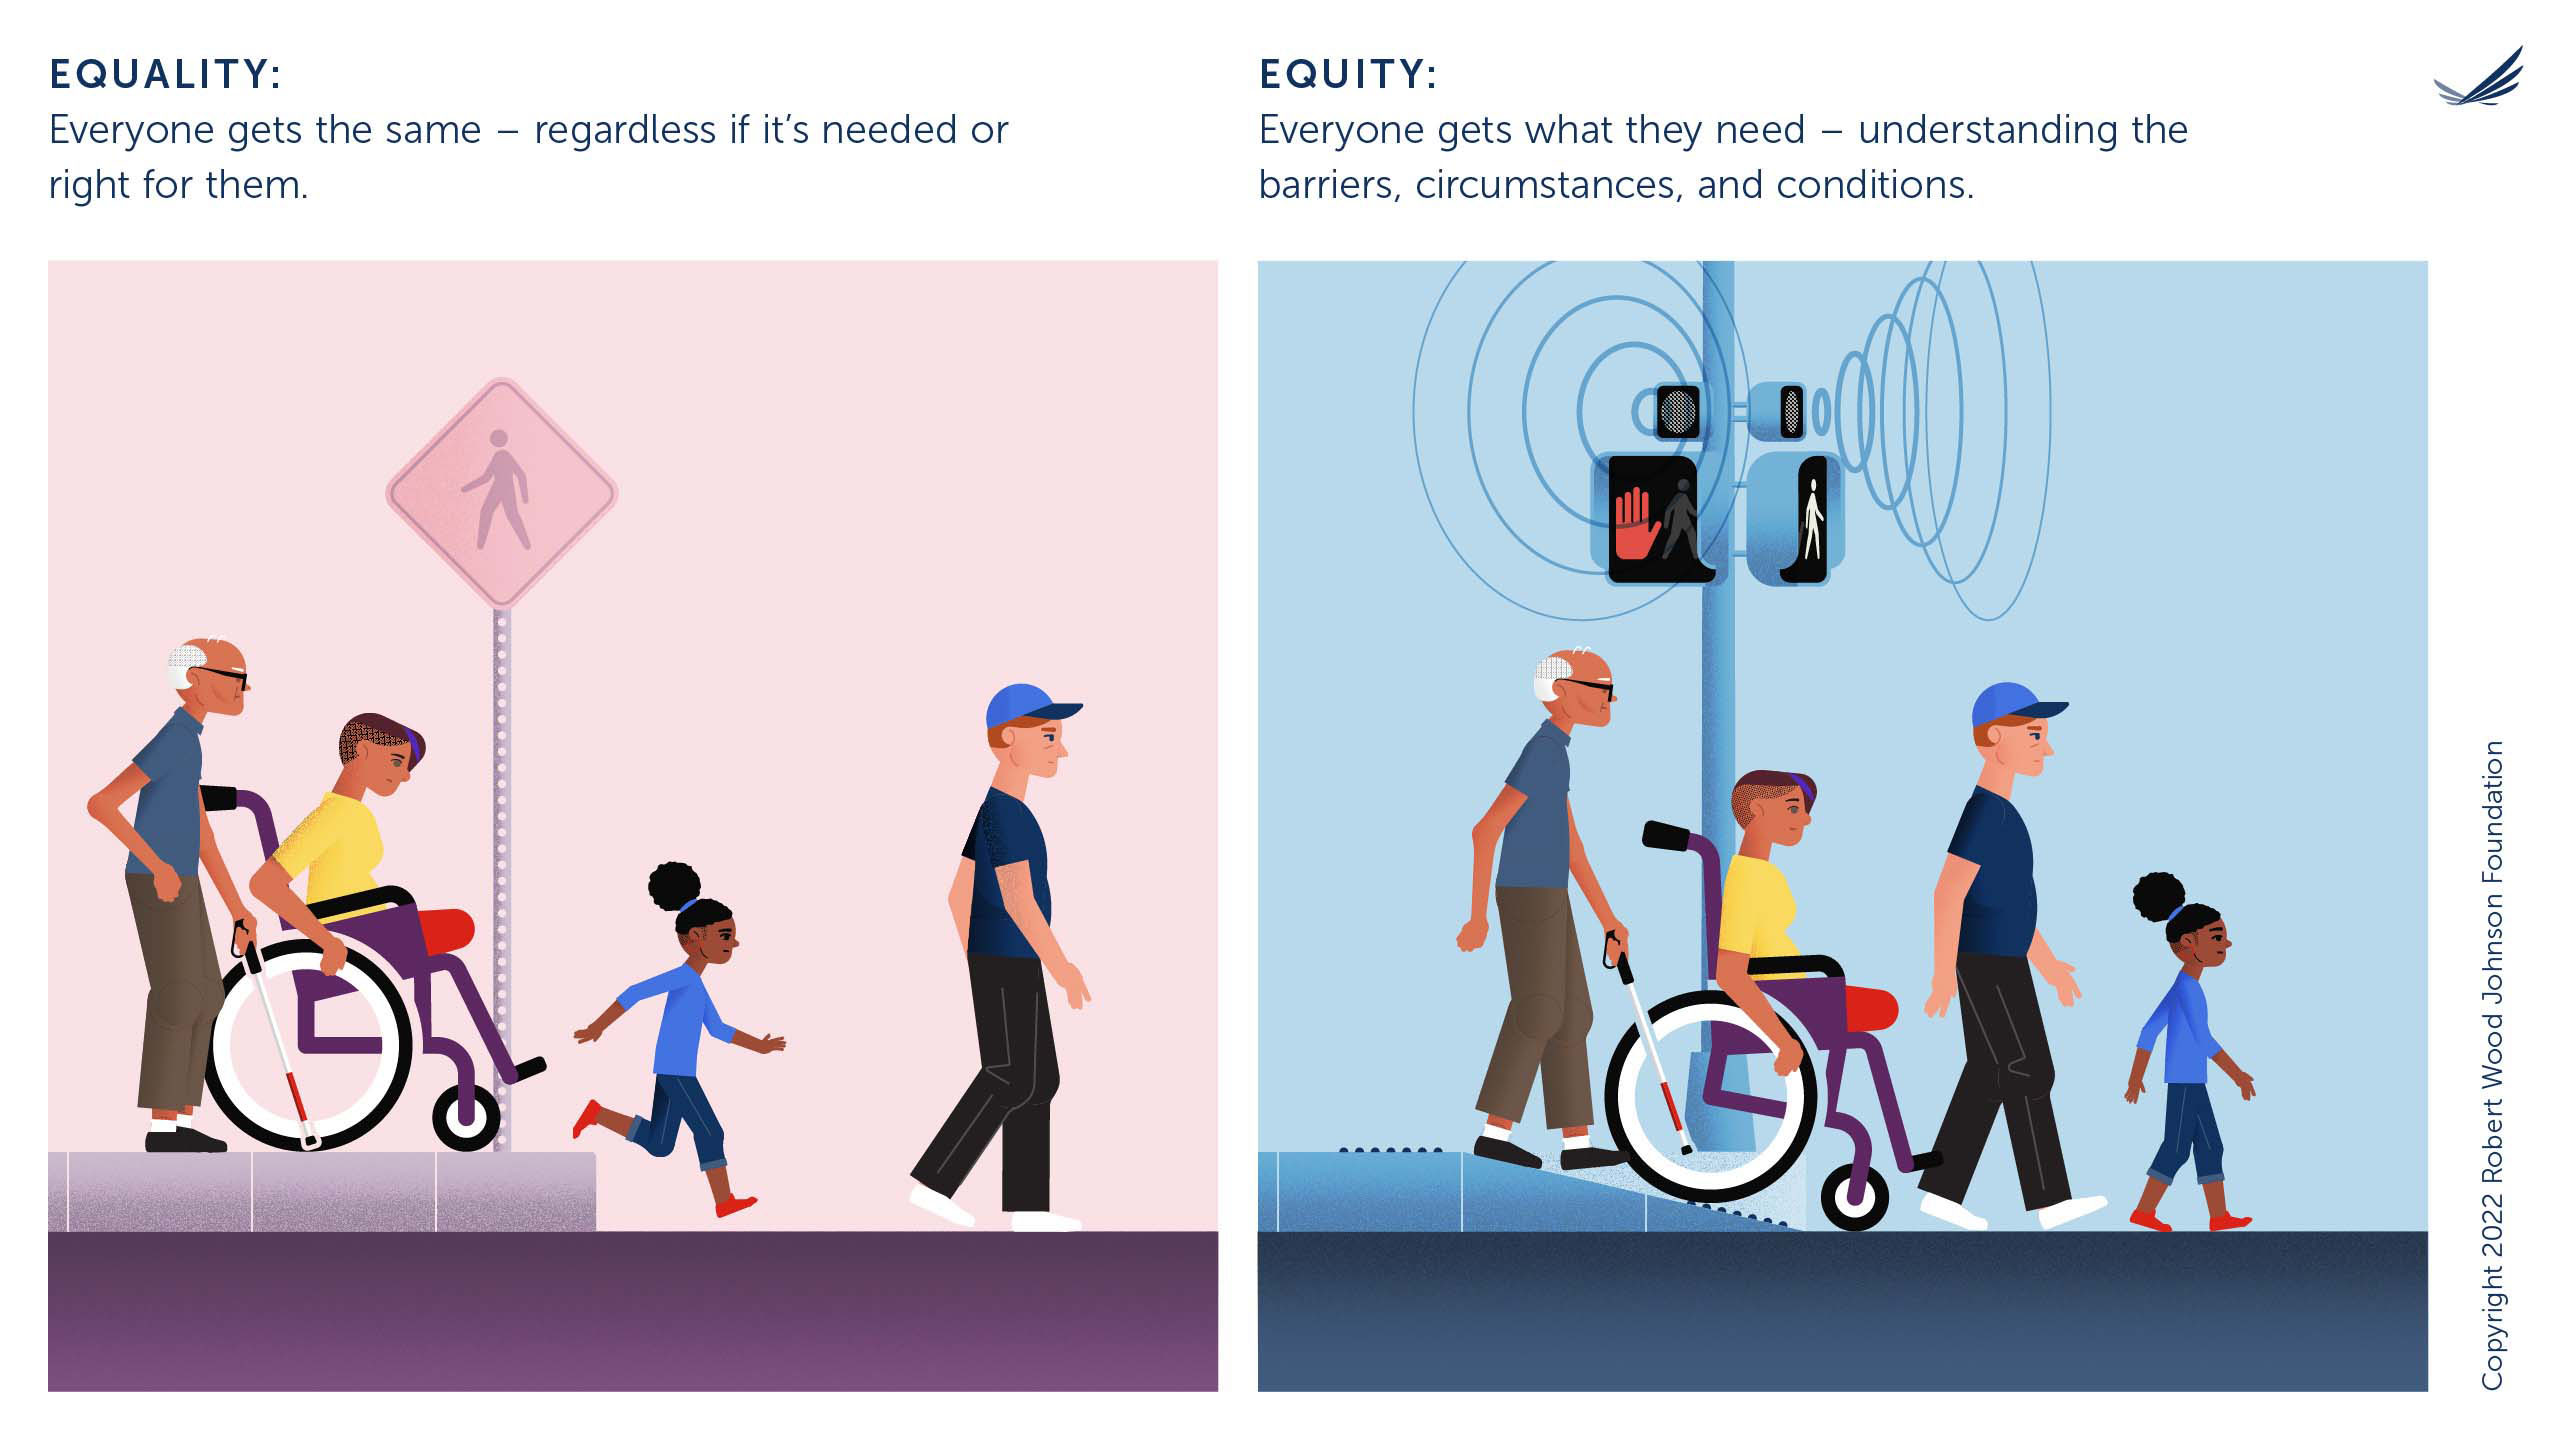
\includegraphics[keepaspectratio]{4_social-sustainability/images/Fig4_6_EqualityEquity.jpg}}

}

\caption{\label{fig-EqualityEquity}Gleichheit
vs.~Gerechtigkeit/Fairness. Quelle: Mit Genehmigung der Robert Wood
Johnson Foundation, Princeton, N.J., reproduziert.}

\end{figure}%

\textbf{Ungleichheit betrachten: Wo und wen?}

Aufbauend auf dem Fähigkeitenansatz, der die realen Möglichkeiten der
Menschen betont, das Leben zu führen, das sie schätzen, ist es
entscheidend anzuerkennen, dass Ungleichheit auf unterschiedliche Weise
manifest werden und über verschiedene Dimensionen hinweg bewertet werden
kann. Ungleichheit kann in verschiedenen Räumen analysiert werden,
beispielsweise durch die Unterscheidung zwischen \textbf{absoluter} und
\textbf{relativer Ungleichheit} (Niño-Zarazúa u.~a. 2017) oder zwischen
\textbf{vertikaler} und \textbf{horizontaler Ungleichheit} (Stewart
2005).

\textbf{Absolute Ungleichheit} beschreibt eine Situation, in der
Menschen nicht in der Lage sind, ihre grundlegendsten
Überlebensbedürfnisse zu erfüllen. Dies ist beispielsweise dann der
Fall, wenn eine Person keinen Zugang zu sauberem Trinkwasser,
ausreichend Nahrung oder sicherem Wohnraum hat und unter der
Armutsgrenze lebt. Diese Form der Ungleichheit wird oft durch feste
Einkommensschwellen definiert, wie z. B. die internationale Armutsgrenze
der Weltbank.

\textbf{Relative Ungleichheit} misst den Nachteil einer Person im
Verhältnis zum durchschnittlichen Lebensstandard innerhalb einer
bestimmten Gesellschaft oder Gemeinschaft. Eine Familie in einem reichen
Land mag beispielsweise über ausreichendes Einkommen für Nahrung und
Wohnraum verfügen, aber möglicherweise nicht über die Ressourcen, um
vollständig an der Gesellschaft teilzunehmen -- wenn sie sich
beispielsweise keinen Internetzugang oder Schulausflüge für ihre Kinder
leisten können. Relative Ungleichheit wird deutlich, wenn die
Lebensbedingungen erheblich unter dem sozialen Durchschnitt liegen. Sie
führt häufig zu sozialer Ausgrenzung und schränkt den Zugang zu
Ressourcen und den Möglichkeiten ein, die notwendig sind, um in einem
bestimmten sozialen Kontext ein würdiges und selbstbestimmtes Leben zu
führen. Der wesentliche Unterschied zwischen den beiden Konzepten
besteht darin, dass \textbf{absolute Armut} einen objektiven Mangel an
wesentlichen Gütern bezeichnet, während \textbf{relative Armut} den
sozialen und wirtschaftlichen Status einer Person im Verhältnis zu
anderen in einer Gesellschaft beschreibt (Niño-Zarazúa u.~a. (2017)).

Ein weiteres Konzept unterscheidet zwischen \textbf{vertikaler} und
\textbf{horizontaler Ungleichheit}. Vertikale Ungleichheit konzentriert
sich auf sozioökonomische Unterschiede zwischen Individuen -- etwa bei
Einkommen, Berufsstatus oder Bildung. Im Gegensatz dazu bezieht sich
horizontale Ungleichheit auf Unterschiede zwischen kulturell definierten
Gruppen, basierend beispielsweise auf Geschlecht, Alter, Familienstand,
Nationalität, Region oder Wohnort (Stewart 2005).

\textbf{Wie analysiert man Ungleichheit? Individuelle vs.~strukturelle
Ansätze}

Analysen von Ungleichheit unterscheiden oft zwischen
\textbf{individueller Ungleichheit} und \textbf{struktureller
Ungleichheit}. Eine Analyse individueller Ungleichheit stützt sich auf
die Prinzipien der Wohlfahrtsökonomie und das Konzept der absoluten
Ungleichheit. Sie konzentriert sich auf sozioökonomische Merkmale wie
Unterschiede in Einkommen, Bildungsstand und Berufsstatus. Dieser Ansatz
geht davon aus, dass wirtschaftliche Ungleichheiten in erster Linie das
Ergebnis persönlicher Eigenschaften und individueller Anstrengungen
sind.

Im Gegensatz dazu orientieren sich Analysen struktureller Ungleichheit
stärker an den Konzepten der Fairness/Gerechtigkeit, des
Fähigkeitenansatzes und der relativen Ungleichheit. Strukturelle
Ungleichheit wird nicht als Produkt der Eigenschaften einer Einzelperson
betrachtet, sondern als Ergebnis des sozialen Rahmens -- wie z. B. der
Position einer Person innerhalb der Produktionsweise oder der sozialen
Hierarchie; ihres Zugangs zu Löhnen, Gewinnen oder einer Rente; oder
ihrer Nationalität, die allesamt Schlüsselfaktoren globaler Ungleichheit
sind (vgl. Milanovic 2019).

Dieses Kapitel hat verschiedene Perspektiven auf Ungleichheit
vorgestellt, darunter den weit verbreiteten Fähigkeitenansatz, der eine
übergreifende und normative Perspektive bietet. Die anderen Perspektiven
mögen ähnlich klingen, unterscheiden sich aber tatsächlich in ihrem
Schwerpunkt (vgl. Tabelle~\ref{tbl-inequality-categories}).

\begingroup\fontsize{8}{10}\selectfont

\begin{longtable}[t]{>{\raggedright\arraybackslash}p{1.6cm}>{\raggedright\arraybackslash}p{2.5cm}>{\raggedright\arraybackslash}p{2.5cm}>{\raggedright\arraybackslash}p{2.5cm}>{\raggedright\arraybackslash}p{2.5cm}}

\caption{\label{tbl-inequality-categories}Kategorien und
Analysedimensionen von Ungleichheit.}

\tabularnewline

\toprule
\textbf{Kategorie} & \textbf{Was wird verglichen?} & \textbf{Schwerpunkt} & \textbf{Typisches Beispiel} & \textbf{Politische Relevanz}\\
\midrule
\endfirsthead
\multicolumn{5}{@{}l}{\textit{(continued)}}\\
\toprule
\textbf{Kategorie} & \textbf{Was wird verglichen?} & \textbf{Schwerpunkt} & \textbf{Typisches Beispiel} & \textbf{Politische Relevanz}\\
\midrule
\endhead

\endfoot
\bottomrule
\endlastfoot
\textbf{relativ vs. absolut} & Im Verhältnis zu Unterschieden gemessene Ungleichheit vs. absolute Unterschiede & Kategorisierung von Ungleichheit: Wer hat mehr/weniger? & Die Wohlhabenden erhalten 40\textbackslash{}\% des Einkommens, während die Armen 10\textbackslash{}\% erhalten (relativ) vs. die zur Deckung von Grundbedürfnissen erforderliche Einkommenslücke (absolut) & Verteilungsgerechtigkeit vs. Armutsbekämpfung\\
\textbf{vertikal vs. horizontal} & Unterschiede zwischen Einkommensniveaus vs. Unterschiede zwischen sozialen Gruppen & Kategorisierung von Ungleichheit: Wie wird Ungleichheit quantifiziert und dargestellt? & Ein CEO verdient 100-mal mehr als eine Reinigungskraft (vertikal) vs. Frauen verdienen weniger als Männer für die gleiche Arbeit (horizontal) & Umverteilung vs. Antidiskriminierung\\
\textbf{individuell vs. strukturell} & Unterschiede aufgrund persönlicher Merkmale vs. Unterschiede aufgrund sozialer Strukturen & Analysedimension von Ungleichheit: Was sind die Ursachen von Ungleichheit? & Individuell: jemand wird durch Talent und Einsatz erfolgreich vs. strukturell: jemand ist aufgrund seiner Herkunft benachteiligt & Förderung der Chancengleichheit vs. Reform sozialer Strukturen\\*

\end{longtable}

\endgroup{}

\section{Sozialer Zusammenhalt}\label{sozialer-zusammenhalt}

\textbf{Sozialer Zusammenhalt} beschreibt das Gefühl der
Zusammengehörigkeit, des Vertrauens und der Kooperationsbereitschaft --
innerhalb von Gruppen, zwischen verschiedenen Gruppen und gegenüber
staatlichen Institutionen. Das Konzept beschreibt, inwieweit Menschen
und Gemeinschaften auf der Grundlage interpersonellen und
institutionellen Vertrauens handeln, welche Einstellungen sie gegenüber
Minderheiten haben und wie sicher sie sich fühlen. Gesellschaften mit
starkem sozialen Zusammenhalt finden sich sowohl in wohlhabenden Ländern
als auch in von Konflikten betroffenen Ländern (Cuesta u.~a. 2024).

Ein funktionierender sozialer Zusammenhalt und das Wohlergehen einer
Bevölkerung erfordern, dass alle sozialen Gruppen wirtschaftlich,
politisch, sozial und kulturell teilhaben können. Dies ist eng mit
Inklusion und Ungleichheit verknüpft. Anstatt sich jedoch auf
Unterschiede zwischen Individuen oder bestimmten Gruppen zu
konzentrieren, fragt das Konzept des sozialen Zusammenhalts, wie stark
die Gesellschaft als Ganzes verbunden ist.

Sozialer Zusammenhalt ist die Grundlage für gegenseitiges Vertrauen und
kollektives Handeln. Er gilt als zentrale Voraussetzung für Frieden und
Wohlstand (Chatterjee u.~a. 2023). Studien zeigen beispielsweise, dass
Gesellschaften mit einem hohen Vertrauensniveau weniger Konflikte
erleben (Putnam 2000; Rothstein und Uslaner 2005). Im Gegensatz dazu ist
geringeres soziales Vertrauen oft mit grösserer wirtschaftlicher
Ungleichheit verbunden (Jordahl 2007) (vgl.
Abbildung~\ref{fig-TrustInequality}).

\begin{figure}[H]

\centering{

\pandocbounded{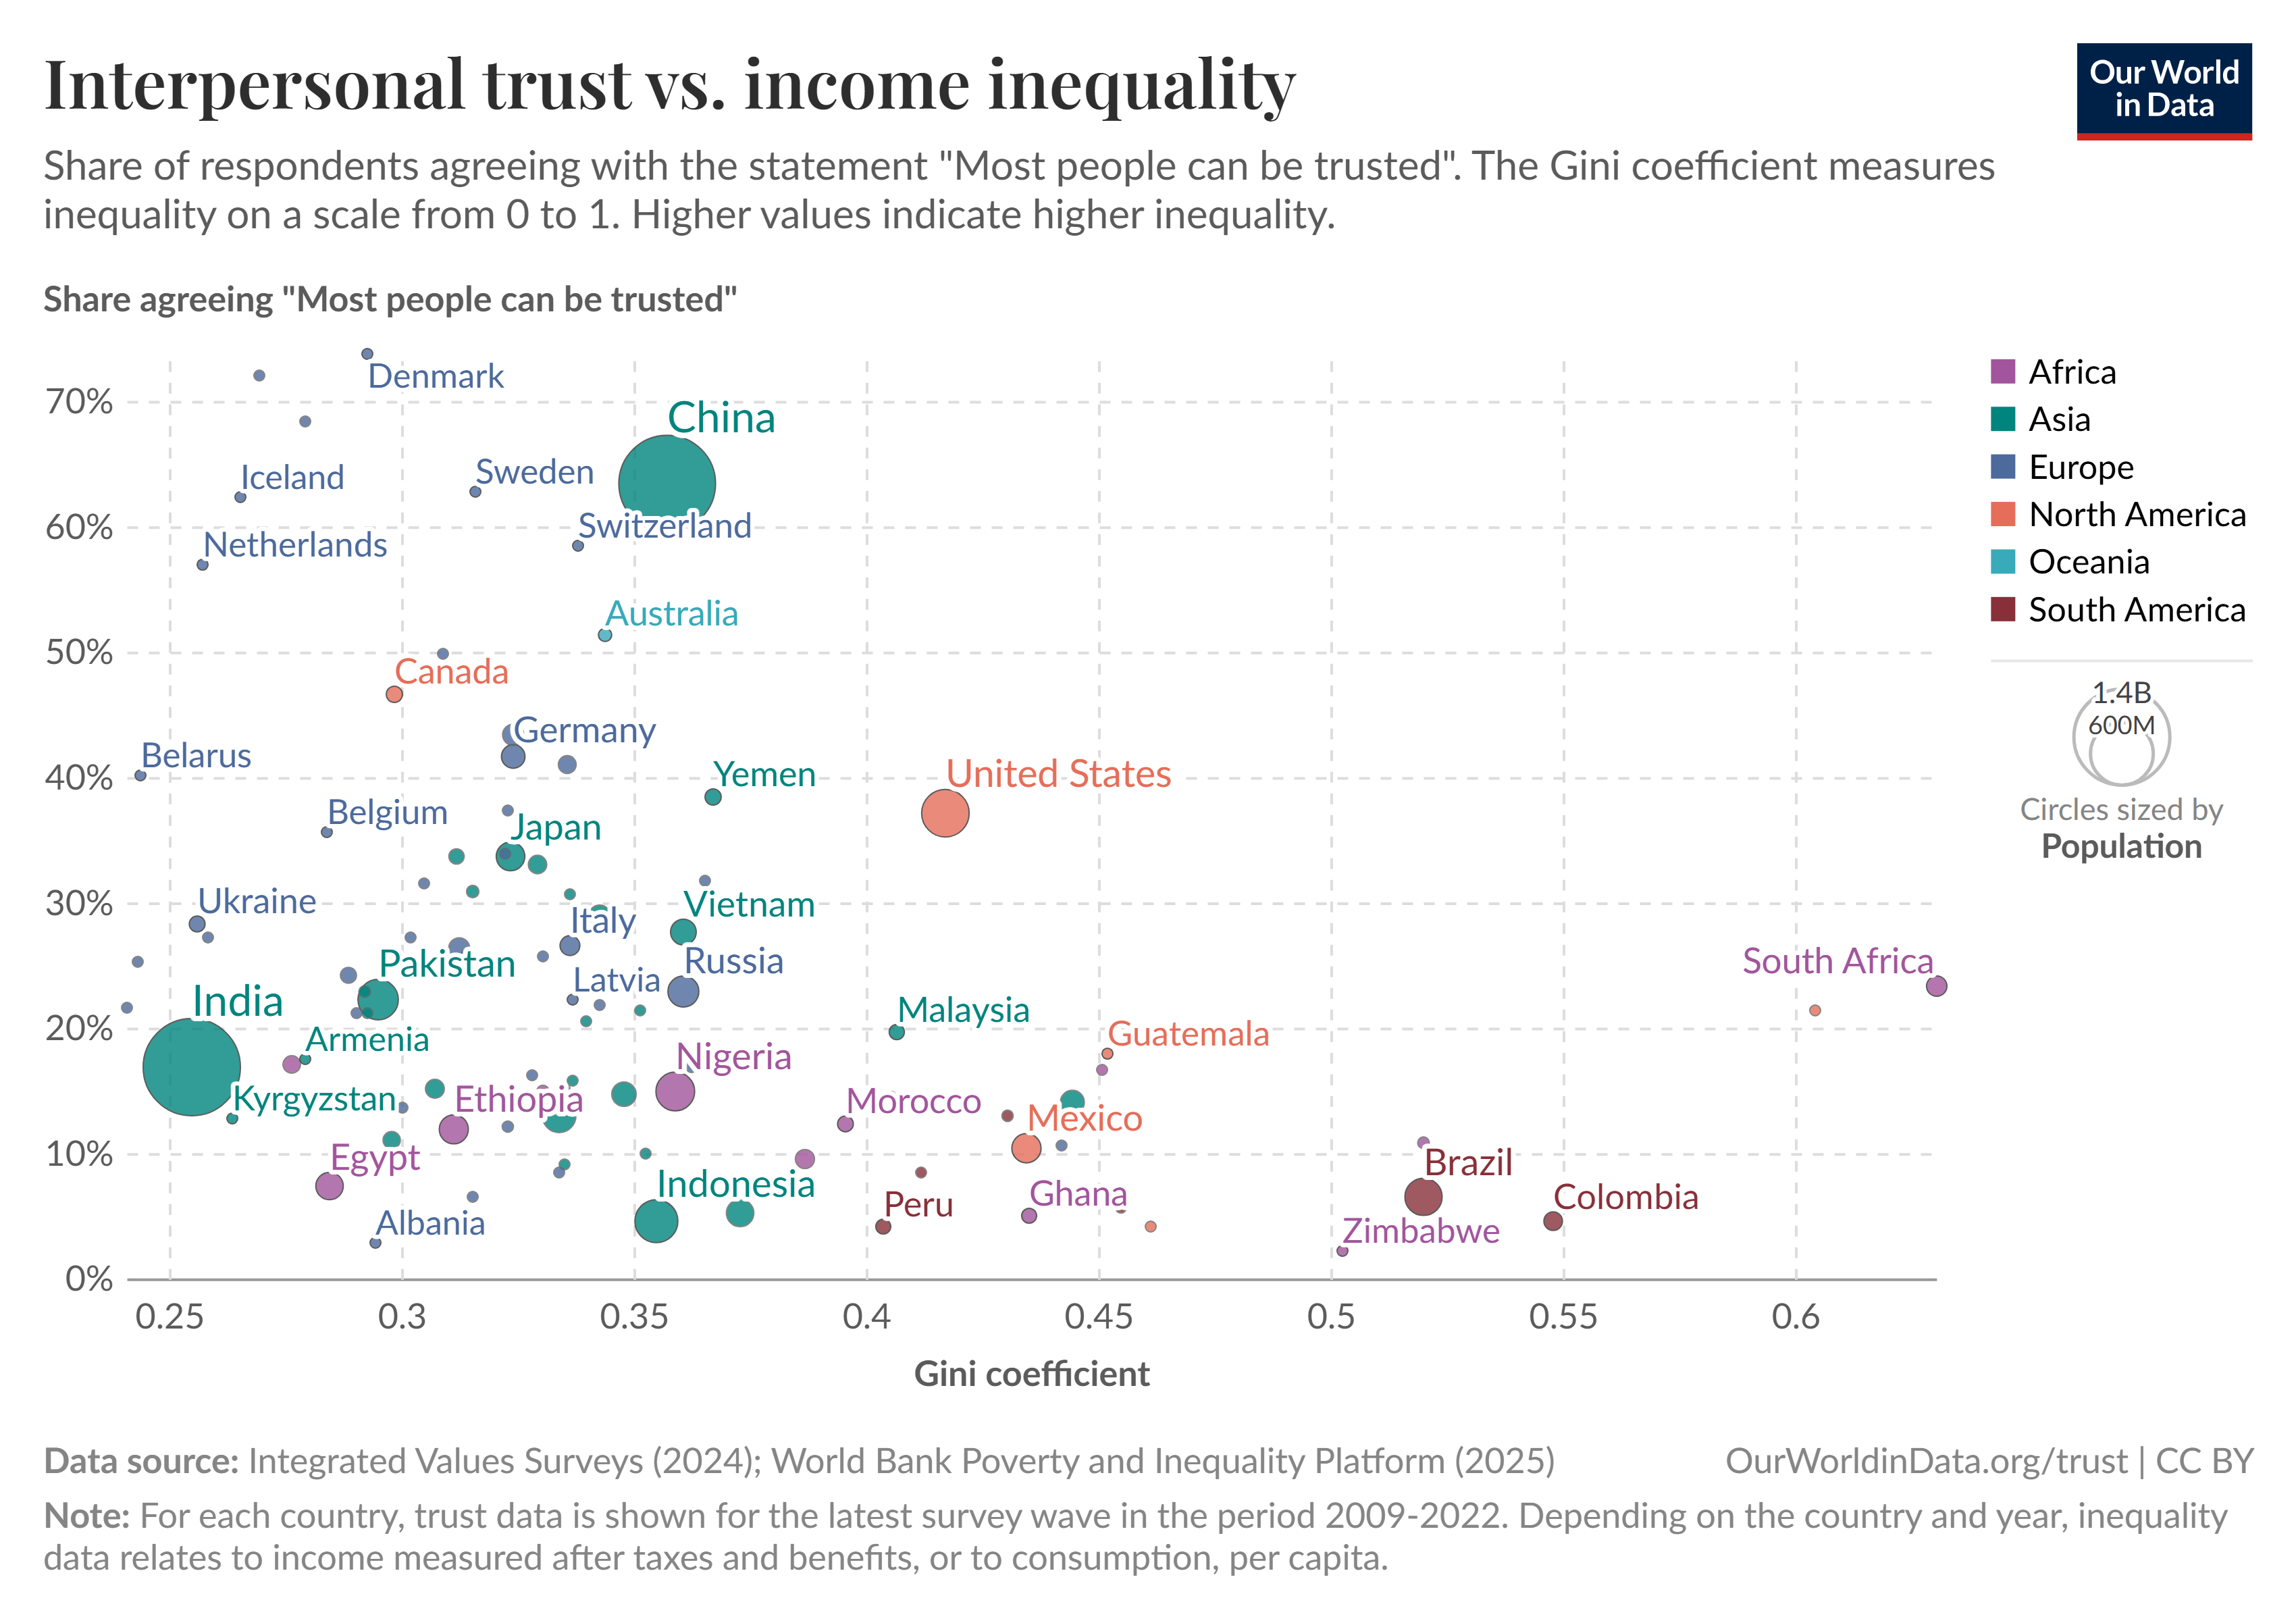
\includegraphics[keepaspectratio]{4_social-sustainability/images/Fig4_7_TrustInequality.png}}

}

\caption{\label{fig-TrustInequality}Interpersonelles Vertrauen
vs.~Einkommensungleichheit. Quelle:
\url{https://ourworldindata.org/grapher/interpersonal-trust-vs-income-inequality}.}

\end{figure}%

Das obige Streudiagramm veranschaulicht den Zusammenhang zwischen
interpersonellem Vertrauen und Einkommensungleichheit. Jeder Punkt
repräsentiert ein Land. Die Punktfarbe kategorisiert Länder nach ihrer
jeweiligen Region; die Punktgrösse spiegelt die Bevölkerungsgrösse des
Landes wider. Die Y-Achse zeigt den Prozentsatz der Bevölkerung eines
Landes, der der Aussage „Den meisten Menschen kann man vertrauen''
zustimmt. Die X-Achse zeigt den Gini-Koeffizienten, ein weit
verbreitetes Mass für Einkommensungleichheit: Ein Wert von 0 entspricht
vollständiger Einkommensgleichheit, während ein Wert von 1 (oder 100\%)
maximale Einkommensungleichheit darstellt -- d.~h. eine einzelne Person
hält das gesamte Einkommen, während alle anderen nichts erhalten.

Das Diagramm zeigt, dass das Niveau des sozialen Vertrauens in Ländern
mit einem höheren Gini-Index tendenziell geringer ist. Eine Erklärung
für die negative Korrelation zwischen Ungleichheit und Vertrauen ist,
dass Menschen tendenziell mehr Vertrauen in diejenigen setzen, die ihnen
ähnlich sind, und dass grössere Ungleichheit zu Spannungen und
Verteilungskonflikten führt (Alesina und La Ferrara 2002). Gleichzeitig
zeigen einige Länder trotz eines niedrigen Gini-Werts ein geringes
Vertrauensniveau (z. B. Slowakei, Kirgisistan und Albanien). Dies deutet
darauf hin, dass zwar ein allgemeiner Trend erkennbar ist, aber keine
Kausalbeziehung besteht und andere Faktoren eine Rolle spielen.

\textbf{Schlüsselelemente des sozialen Zusammenhalts}

Abbildung~\ref{fig-TrustInequality} ist nur ein Beispiel für sozialen
Zusammenhalt. Das Konzept ist schwer präzise zu definieren, da die
wissenschaftliche Literatur hinsichtlich seiner genauen Bedeutung und
Messung variiert. Dennoch können drei Schlüsselelemente identifiziert
werden ({Schiefer und van der Noll} 2017):

\begin{enumerate}
\def\labelenumi{\arabic{enumi}.}
\item
  \textbf{Soziale Beziehungen}: Netzwerke, Vertrauen, Akzeptanz von
  Vielfalt und Teilhabe
\item
  \textbf{Identifikation mit der Gesellschaft}: emotionale Bindung an
  die soziale Gemeinschaft
\item
  \textbf{Orientierung am Gemeinwohl}: Verantwortungsbewusstsein,
  Solidarität und Einhaltung sozialer Regeln.
\end{enumerate}

Sozialer Zusammenhalt spiegelt sich in den Einstellungen und im
Verhalten aller sozialen Gruppen wider und umfasst sowohl normative als
auch relationale Dimensionen. Er sollte als Kontinuum verstanden werden,
entlang dessen Gesellschaften unterschiedliche Grade des Zusammenhalts
aufweisen können.

Um zu veranschaulichen, wie diese Elemente operationalisiert werden,
lohnt ein Blick darauf, wie sozialer Zusammenhalt in der Schweiz
gemessen wird, wo er eine besondere Bedeutung hat: Die Förderung des
„inneren Zusammenhalts'' ist in der Bundesverfassung als Ziel der
Schweizerischen Eidgenossenschaft verankert (Art. 2). Eine entscheidende
Rolle bei der Verbindung der Menschen in der mehrsprachigen Schweiz
spielt die Kultur, die als „gesellschaftlicher Kitt'' wirkt. Obwohl
sozialer Zusammenhalt in der Agenda 2030 kein explizites Ziel ist, wird
er implizit in mehreren ihrer Zielvorgaben angesprochen. In der Schweiz
wird sozialer Zusammenhalt vom Bundesamt für Statistik anhand einer
Reihe von Indikatoren definiert und gemessen
vgl.~\ref{tbl-social-cohesion-switzerland}.

Das erste Element, \textbf{soziale Beziehungen}, zeigt sich in der
politischen Teilhabe, etwa beim Wählen und Abstimmen. Dieses Element
umfasst auch die kulturelle Teilhabe, die als Anteil der Bevölkerung
gemessen wird, der an kulturellen Aktivitäten teilnimmt. Soziale
Beziehungen werden durch Faktoren wie Diskriminierung negativ
beeinflusst, die das Vertrauen der Menschen in Mitmenschen und
Institutionen sowie das Zugehörigkeitsgefühl zu einem sozialen Netzwerk
untergräbt.

Das zweite Element, \textbf{Identifikation mit der Gesellschaft}, kann
sich darin zeigen, wie Menschen die regionale Gleichheit wahrnehmen. In
der Schweiz misst das Bundesamt für Statistik beispielsweise finanzielle
Unterschiede zwischen den Kantonen. Mehrsprachigkeit ist ebenfalls
relevant: Die Fähigkeit, mit verschiedenen Sprachgemeinschaften zu
kommunizieren, kann das Zugehörigkeitsgefühl stärken und das
interkulturelle Verständnis fördern.

Das dritte Element, \textbf{Orientierung am Gemeinwohl}, umfasst Aspekte
der sozialen Teilhabe, insbesondere auf dem Arbeitsmarkt. Dazu gehören
beispielsweise die Erwerbsquote von Menschen mit Behinderungen oder die
Arbeitslosenquote nach Migrationsstatus -- Indikatoren für strukturelle
Inklusion und Solidarität. Soziale Ungleichheiten sind hier ebenfalls
zentral, gemessen etwa durch die Armuts- oder Armutsrisikoquote in der
Erwerbsbevölkerung. Ein weiterer wichtiger Indikator ist das
zivilgesellschaftliche Engagement, insbesondere durch ehrenamtliche
Arbeit, das ein direktes Mass für soziale Verantwortung und
Gemeinschaftssinn darstellt.

\textbf{Bildung} ist ein Querschnittsthema, das alle drei Elemente
betrifft: Bildung fördert soziale Beziehungen, stärkt die Identifikation
mit der Gesellschaft und unterstützt die Orientierung am Gemeinwohl,
indem soziale Normen und Werte vermittelt werden. Relevante Indikatoren
umfassen die Abschlussquote der Sekundarstufe II und den Anteil junger
Menschen, die weder in Ausbildung noch in Beschäftigung sind.

\begingroup\fontsize{8}{10}\selectfont

\begin{longtable}[t]{>{\raggedright\arraybackslash}p{5.5cm}>{\raggedright\arraybackslash}p{5.5cm}}

\caption{\label{tbl-social-cohesion-switzerland}Messung des sozialen
Zusammenhalts in der Schweiz.}

\tabularnewline

\toprule
\textbf{Schlüsselelement (Schiefer und van der Noll 2017)} & \textbf{Indikatoren (FSO 2025)}\\
\midrule
\endfirsthead
\multicolumn{2}{@{}l}{\textit{(continued)}}\\
\toprule
\textbf{Schlüsselelement (Schiefer und van der Noll 2017)} & \textbf{Indikatoren (FSO 2025)}\\
\midrule
\endhead

\endfoot
\bottomrule
\endlastfoot
\textbf{Soziale Beziehungen} & • Politische Teilhabe (z. B. Wahlen und Abstimmungen)\newline • Kulturelle Teilhabe\newline • Erfahrung von Diskriminierung\\
\textbf{Identifikation mit der Gesellschaft} & • Regionale Unterschiede (z. B. Finanzkraft der Kantone)\newline • Mehrsprachigkeit/kulturelle Integration\\
\textbf{Orientierung am Gemeinwohl} & • Arbeitsmarktbeteiligung (z. B. Erwerbsquote von Menschen mit Behinderungen)\newline • Soziale Ungleichheit (z. B. Armutsniveau)\newline • Ehrenamtliche Arbeit\\
\textbf{Querschnittsthema} & • Bildung\\*

\end{longtable}

\endgroup{}

\section{Resilienz}\label{resilienz}

\textbf{Resilienz} ist die Fähigkeit von Einzelpersonen, Haushalten,
Gemeinschaften oder ganzen Gesellschaften, sich auf Schocks
vorzubereiten, damit umzugehen und sich davon zu erholen (Folke 2016).
Schocks können auf individueller Ebene auftreten (z. B. Jobverlust,
Krankheit) oder auf gesellschaftlicher Ebene (z. B. Naturkatastrophen,
Konflikte, Nahrungsmittelknappheit). Sie können plötzlich eintreten (z.
B. Naturkatastrophen), sich schrittweise intensivieren (z. B.
Bodendegradation) oder ein dauerhaftes Phänomen sein (z. B. Armut,
Kinderarbeit, geschlechtsbezogene Gewalt).

Gesellschaften mit einem hohen Mass an Resilienz können ihre
Lebensqualität und wirtschaftliche Stabilität nach einem Schock
schneller wiedererlangen. Resilienz ist besonders wichtig für arme und
marginalisierte Gruppen, da sie mehr Schocks ausgesetzt sind, grössere
relative Verluste erleiden und weniger Unterstützung erhalten (Bangalore
u.~a. 2017). Ungleichheiten bedeuten auch, dass verschiedene Gruppen von
Schocks ungleich oder unverhältnismässig stark betroffen sind
(Hallegatte u.~a. 2020). Je nach sozialen Normen sind Gruppen wie
Frauen, junge Menschen oder ältere Menschen oft gefährdeter oder weniger
anpassungsfähig (Ajibade u.~a. 2013; Barrett u.~a. 2021).

Es lassen sich drei unterschiedliche Strategien zur Bewältigung von
Risiken und zum Aufbau von Resilienz identifizieren:

\begin{enumerate}
\def\labelenumi{\arabic{enumi}.}
\item
  \textbf{Risikoreduzierung und -minderung}: Massnahmen, die die
  Wahrscheinlichkeit von Schocks oder deren negative Folgen verringern
  (Obrist u.~a. 2010). Beispiele umfassen Impfungen,
  Einkommensdiversifizierung, lokale Schutzinfrastruktur oder staatliche
  Sozialsysteme.
\item
  \textbf{Bewältigungsstrategien}: Reaktionen auf Schocks (Imperiale und
  Vanclay 2021; Severi u.~a. 2012). Bewältigungsstrategien umfassen
  Versicherungsmodelle, den Rückgriff auf Ersparnisse oder Kredite sowie
  die Unterstützung durch soziale Netzwerke. Auch Regierungen können
  helfen, beispielsweise durch Geldtransfers oder Sozialprogramme. Ohne
  ausreichende Ressourcen können von Schocks betroffene Menschen jedoch
  zu schädlichen, kurzfristigen Massnahmen greifen, wie z. B. die
  Einschränkung des wesentlichen Konsums, Übernutzung von Ressourcen
  oder Einsatz von Kinderarbeit.
\item
  \textbf{Transformative Strategien}: Weitreichende Reformen oder neue
  Institutionen, die die langfristige Resilienz von Gesellschaften
  stärken (Mozumder u.~a. 2018; Pfefferbaum u.~a. 2017), typischerweise
  durch die Kombination von Risikoreduzierungs- und
  Bewältigungsstrategien. Beispiele sind die Einrichtung einer
  staatlichen Behörde für die Hochwasservorsorge, die Frühwarnsysteme
  verbessert, die Risikoreduzierungsforschung fördert und
  Hochwasserbewältigungspläne entwickelt. Oder die Einführung von
  Massnahmen zur Verringerung des Risikos geschlechtsbezogener Gewalt
  durch Investitionen in rechtliche, institutionelle und
  Sensibilisierungsprogramme, die Anreize und soziale Normen
  hinsichtlich Gewalt verändern.
\end{enumerate}

\subsection{Grundbedürfnisse als Voraussetzung für
Resilienz}\label{grundbeduxfcrfnisse-als-voraussetzung-fuxfcr-resilienz}

Im oben erwähnten Rahmen der Donut-Ökonomik ist Resilienz nur möglich,
wenn alle Menschen ihre Grundbedürfnisse erfüllen können. Die Erfüllung
dieser sozialen Grundlagen stellt sicher, dass Einzelpersonen und
Gesellschaften besser in der Lage sind, mit Schocks umzugehen. In
Ländern des Globalen Südens sind diese Grundbedürfnisse jedoch häufig
nicht erfüllt. Umgekehrt sind wohlhabendere Länder zwar in der Lage,
diese Bedürfnisse zu erfüllen, überschreiten dabei aber in der Regel
planetare Grenzen. Vgl. Abbildung~\ref{fig-Switzerland}, das die Schweiz
und Laos vergleicht.

\begin{figure}[H]

\begin{minipage}[t]{0.50\linewidth}

\centering{

\pandocbounded{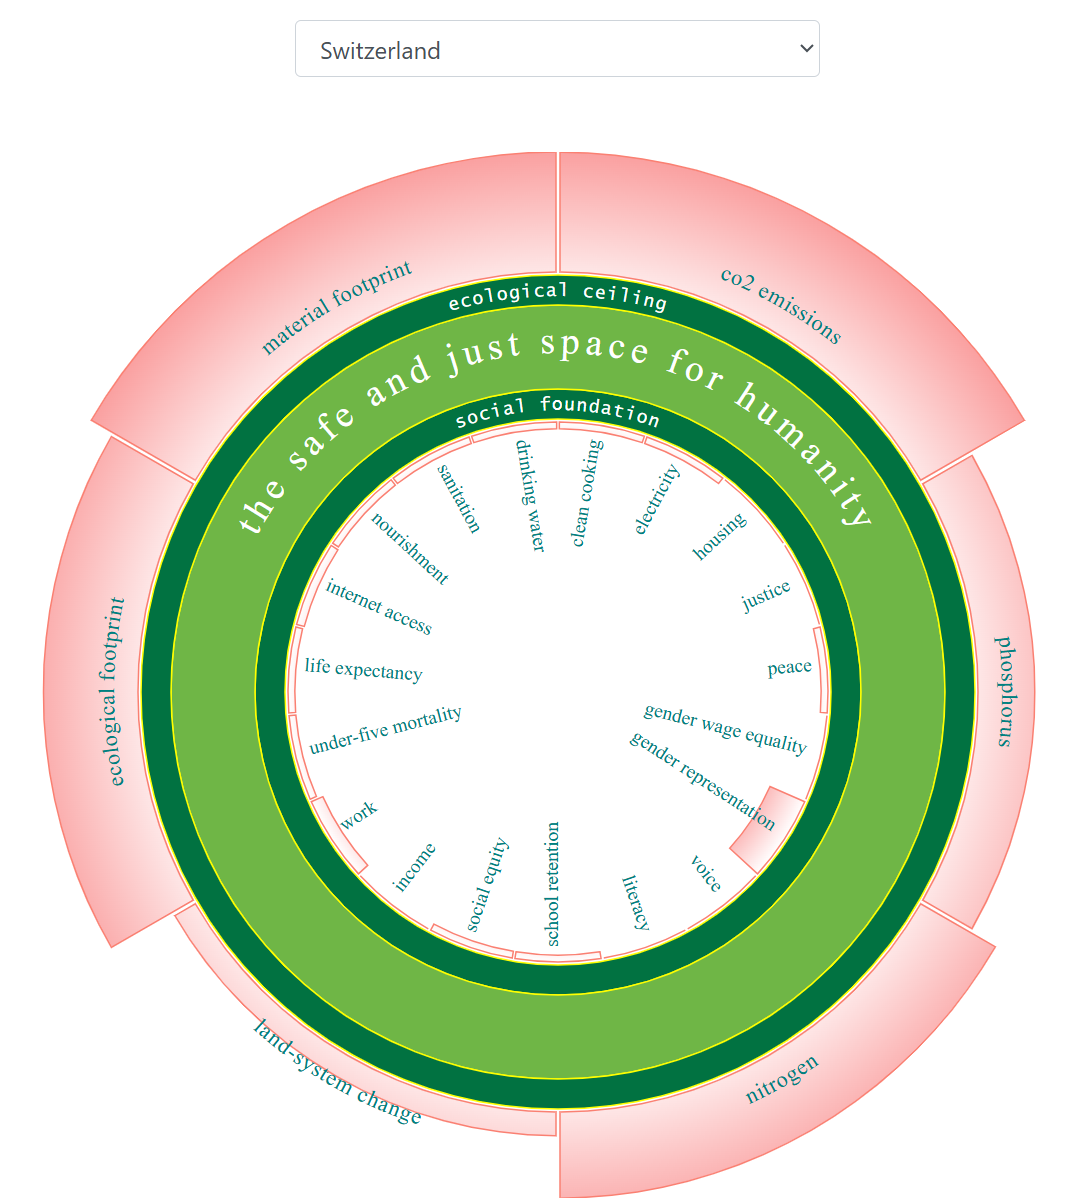
\includegraphics[keepaspectratio]{4_social-sustainability/images/Fig4_8_DoughnutA.png}}

}

\subcaption{\label{fig-Switzerland}Schweiz}

\end{minipage}%
%
\begin{minipage}[t]{0.50\linewidth}

\centering{

\pandocbounded{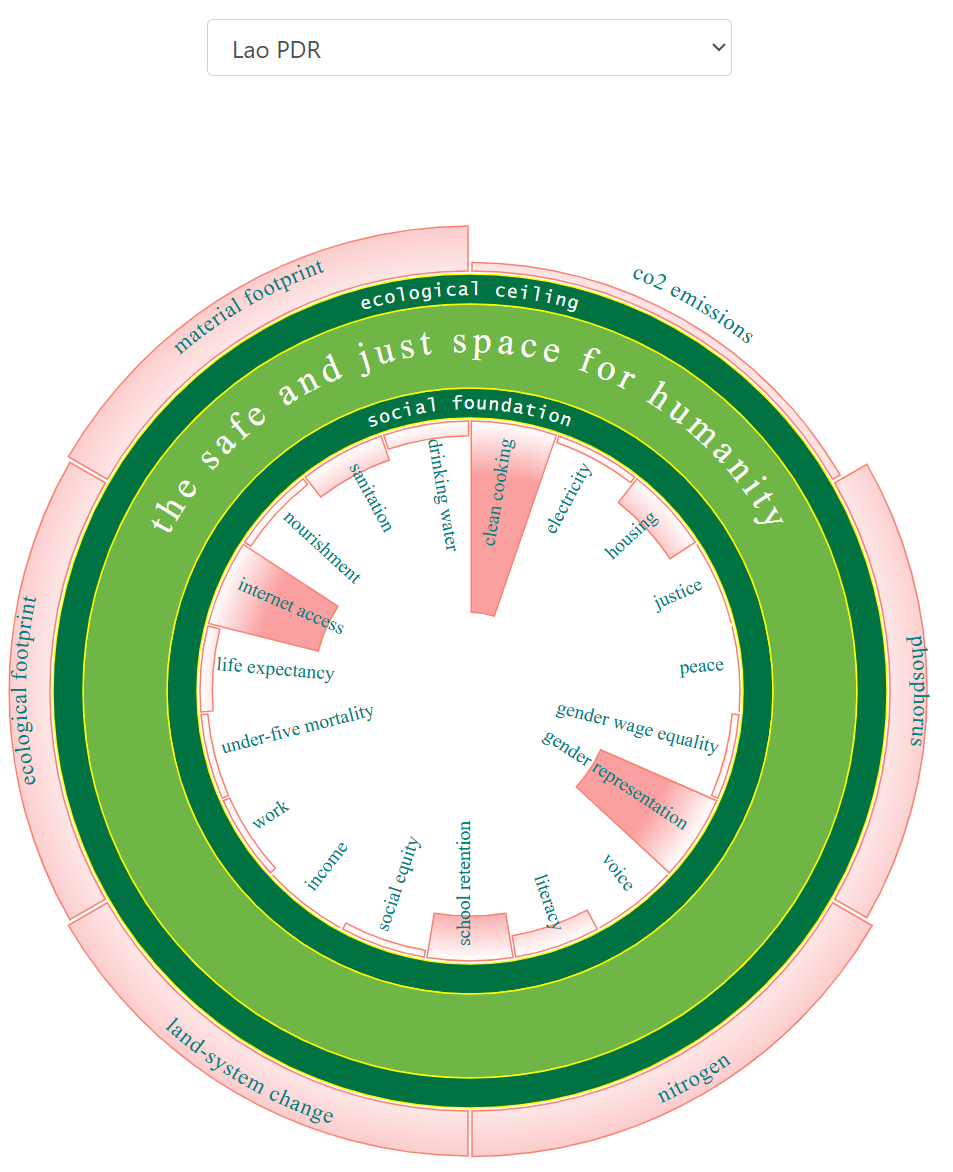
\includegraphics[keepaspectratio]{4_social-sustainability/images/Fig4_8_DoughnutB.png}}

}

\subcaption{\label{fig-laos}Laos}

\end{minipage}%

\caption{\label{fig-elephants}Donut-Visualisierung für die Schweiz
(links) und die Demokratische Volksrepublik Laos (rechts), die die
Leistung jedes Landes in Bezug auf sein soziales Fundament und seine
ökologische Decke vergleicht. Der grüne Donut stellt den sicheren und
gerechten Raum dar, in dem sowohl ökologische als auch soziale Grenzen
respektiert werden. Rote Bereiche zeigen das Ausmass der ökologischen
Überschreitung oder der Defizite bei der Erfüllung sozialer Bedürfnisse
an und zeigen, wo jedes Land ökologische Grenzen überschreitet oder
unter die minimalen sozialen Schwellenwerte fällt. Quelle: Kate Raworth
and Christian Guthier. CC-BY-SA 4.0,
https://doughnut-economy-fxs7576.netlify.app/}

\end{figure}%

Diese Mindestsozialstandards -- der „soziale Boden'' -- umfassen Zugang
zu Nahrung, Gesundheit, Bildung, Einkommen und Arbeit. Dazu gehören auch
Frieden, Gerechtigkeit, politische Teilhabe, soziale und
Geschlechtergleichstellung, Wohnraum, soziale Netzwerke, Energie und
Wasser. In diesem Lehrbuch verwenden wir das Beispiel \textbf{Nahrung},
um zu zeigen, wie der Zugang zu einem dieser Standards die Resilienz
beeinflusst. Schwierigkeiten mit einem einzelnen Standard treten selten
isoliert auf und betreffen häufig auch andere Bereiche. Die
Sicherstellung dieser sozialen Grundlagen ist daher entscheidend für
eine nachhaltige Entwicklung.

\textbf{Globale Ernährungssicherheit}

Ernährungssicherheit bedeutet, ausreichend Nahrung und zuverlässigen
Zugang dazu zu haben, insbesondere zu Grundnahrungsmitteln. Ein Haushalt
gilt als ernährungssicher, wenn seine Mitglieder nicht von Hunger oder
Unterernährung bedroht sind. Unterernährung hat schwerwiegende
gesundheitliche Folgen wie Auszehrung und Wachstumsverzögerung. Sie
erhöht auch die Gesundheitskosten, verringert die Produktivität und
hemmt das Wirtschaftswachstum und verstärkt damit einen Kreislauf aus
Armut und Krankheit.

Ernährungssicherheit ist eng mit der Resilienz eines Ernährungssystems
verknüpft -- seiner Fähigkeit, Veränderungen zu tolerieren und sich
anzupassen. Unser globales Ernährungssystem ist aufgrund seiner
Komplexität und der vielen Interdependenzen zwischen seinen Elementen
besonders anfällig. Es ist sowohl äusseren Bedrohungen -- wie den Folgen
des Klimawandels -- als auch internen Risiken ausgesetzt, wie
politischen Fehlern, nicht nachhaltigen Konsummustern oder
Marktversagen.

Abbildung~\ref{fig-FoodInsecurity} zeigt, dass im Jahr 2022 weltweit
fast 2,4 Milliarden Menschen von Ernährungsunsicherheit betroffen waren.
Knapp die Hälfte davon (1,1 Milliarden) lebte in Asien, 37 Prozent (868
Millionen) in Afrika, 10,5 Prozent (248 Millionen) in Lateinamerika und
der Karibik und rund 4 Prozent (90 Millionen) in Nordamerika und Europa.
Die Abbildung zeigt auch die Anteile schwerer und moderater
Ernährungsunsicherheit: Schwere Ernährungsunsicherheit bedeutet, dass
Menschen Schwierigkeiten haben, ihren kurzfristigen Grundnahrungsbedarf
zu decken. Moderate Ernährungsunsicherheit hingegen bezeichnet eine
unzureichende Versorgung mit wesentlichen Nährstoffen, die zu
gesundheitlichen Problemen führen kann.

\begin{figure}[H]

\centering{

\pandocbounded{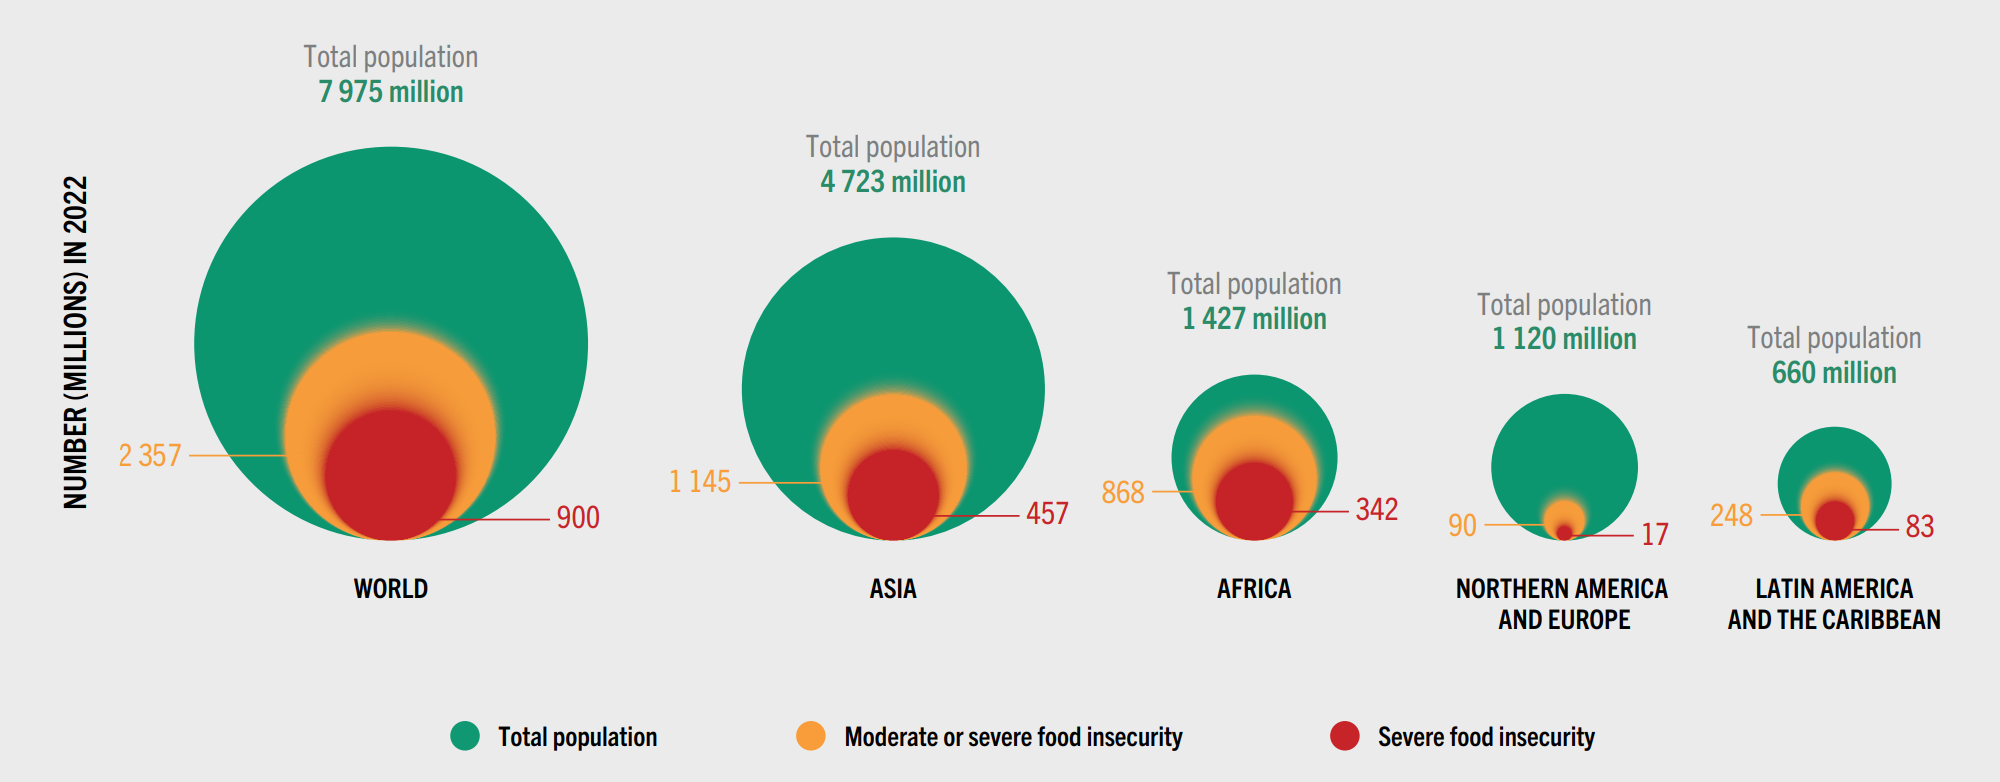
\includegraphics[keepaspectratio]{4_social-sustainability/images/Fig4_9_FoodInsecurity.png}}

}

\caption{\label{fig-FoodInsecurity}Die Konzentration und Verteilung der
Ernährungsunsicherheit nach Schweregrad unterscheiden sich stark
zwischen den Regionen der Welt. Quelle: FAO u.~a. (2023). FAOSTAT: Suite
of Food Security Indicators, www.fao.org/faostat/en/\#data/FS}

\end{figure}%

Dies verdeutlicht den Bedarf an fairen und resilienten
Ernährungssystemen. Wie Abbildung~\ref{fig-FoodInsecurity} zeigt,
umfasst ein Ernährungssystem alle Aktivitäten, Akteure und
Infrastrukturen, die an der Produktion, Verarbeitung, dem Transport, der
Verteilung, dem Handel, dem Konsum und der Entsorgung von Lebensmitteln
beteiligt sind. Ernährungssysteme sind tief in Gesellschaft und Umwelt
eingebettet. Veränderungen innerhalb dieser Systeme betreffen daher
zahlreiche Bereiche: die Umwelt (Wasser, Luft, Boden, Biodiversität),
soziale und kulturelle Aspekte (z. B. Auswirkungen auf lokale
Gemeinschaften), die Wirtschaft (Wertschöpfungsketten, Handel,
Finanzierung) und die Gesundheit (Tribaldos und Kortetmäki 2022b).

Diskussionen zur Bekämpfung von Ernährungsunsicherheit konzentrieren
sich häufig auf die Steigerung der Erträge und die Reduzierung von
Lebensmittelabfällen, doch diese Ansätze erweisen sich nicht als die
wirksamsten. Die aktuellen Nahrungsmittelproduktions- und
-konsumgewohnheiten basieren zunehmend auf hochverarbeiteten Fleisch-
und Milchprodukten sowie auf intensiven Produktionsmethoden. Der globale
Konsum führt zu ausgelagerten Umweltauswirkungen wie Bodendegradation,
Biodiversitätsverlust, Wasserübernutzung und dem Verschwinden lokaler
Pflanzensorten -- Auswirkungen, die in erster Linie die Produzent*innen
und nicht die Konsument*innen betreffen.

Sich allein auf die Steigerung der Produktion zu konzentrieren,
übersieht auch die Tatsache, dass die Welt bereits genug Nahrung
produziert. Was stattdessen benötigt wird, ist eine weitreichende
Transformation darin, wie diese Ressourcen genutzt und verteilt werden.
Shepon u.~a. (2018) fand beispielsweise heraus, dass pflanzliche
Ersatzprodukte, die ernährungsphysiologisch vergleichbar sind (z. B.
hinsichtlich des Proteingehalts), deutlich effizienter sind als
tierische Produkte: Auf einem Hektar Ackerland kann bis zu 20 Mal mehr
Nahrung produziert werden als mit Rindfleisch und doppelt so viel wie
mit Eiern, die das ressourcenintensivste bzw. am wenigsten
ressourcenintensive tierische Lebensmittel darstellen.

Das aktuelle Ernährungssystem verfüttert jedoch grosse Mengen an
essbaren Nutzpflanzen an Nutztiere. Laut Berners-Lee u.~a. (2018) werden
rund 41\% der für Menschen essbaren Nutzpflanzen (gemessen in
Kilokalorien pro Person und Tag) an Nutztiere verfüttert. Dieser Prozess
ist hochgradig ineffizient: Die Tiere geben nur rund 12\% dieser Energie
in Form von Fleisch, Fisch und Milchprodukten zurück. Mit anderen
Worten: Ein erheblicher Anteil potenzieller Nahrung für den menschlichen
Konsum geht dabei verloren (vgl. Abbildung~\ref{fig-GlobalFood}).

\begin{figure}[H]

\centering{

\pandocbounded{\includegraphics[keepaspectratio]{4_social-sustainability/images/Fig4_10_GlobalFoodSupply.png}}

}

\caption{\label{fig-GlobalFood}Die Flüsse globaler Nahrungsenergie
(kcal/Person/Tag) zeigen den Weg von der produzierten Nahrung bis zur
tatsächlich konsumierten Nahrung im Jahr 2013. Für an Tiere verfütterte
Nutzpflanzen basieren die Einheiten auf der Weltbevölkerung, nicht auf
der Tierpopulation. Der linke Balken unterscheidet zwischen
Nutzpflanzen, die direkt für Menschen essbar sind, und Futterpflanzen
wie Gras, Weide oder Ernterückständen, die nur von Tieren genutzt werden
können. Tierverluste (grauer Balken) umfassen alle Energieverluste in
der Tierhaltung, beispielsweise durch Atmung, Wachstum, Bewegung und
Fortpflanzung sowie durch Tierbestandteile, die nicht als Nahrung
genutzt werden. Der äusserste rechte Balken unterteilt die konsumierten
Nährstoffe in den für ein gesundes menschliches Leben erforderlichen
Anteil und zeigt einen kleinen Nettoanstieg des Nahrungsmittelkonsums im
Jahr 2014. Quelle: Berners-Lee u.~a. (2018), lizenziert unter Creative
Commons CC BY.}

\end{figure}%

\section{Gerechtigkeit}\label{sec-justice}

\subsection{Verfahrensgerechtigkeit}\label{verfahrensgerechtigkeit}

\textbf{Inklusion, sozialer Zusammenhalt und Resilienz} gelten als die
drei Schlüsseldimensionen sozialer Nachhaltigkeit. Ob diese Faktoren
tatsächlich soziale Nachhaltigkeit ermöglichen, hängt jedoch von einem
vierten Element ab: der \textbf{Verfahrensgerechtigkeit}.
Verfahrensgerechtigkeit ist entscheidend dafür, ob und in welchem Masse
sozialer Wandel in den drei Dimensionen gelingt.

Verfahrensgerechtigkeit konzentriert sich auf den Prozess. Sie
beschreibt, \emph{wie} Politiken entwickelt, Programme gestaltet und
Massnahmen umgesetzt werden. Ein hohes Mass an Verfahrensgerechtigkeit
wird erreicht, wenn Entscheidungsprozesse als fair, vertrauenswürdig und
mit sozialen Normen übereinstimmend wahrgenommen werden (Hinsch 2016;
Wijsman und Berbés-Blázquez 2022), auch wenn dabei Konflikte und
Spannungen angesprochen werden. Es handelt sich nicht um eine
Entweder-oder-Situation, sondern um ein Kontinuum: Prozesse können als
mehr oder weniger legitim wahrgenommen werden, und verschiedene Gruppen
nehmen dies oft unterschiedlich wahr.

Legitimität zu gewährleisten erfordert die öffentliche Wahrnehmung, dass
Entscheidungen von vertrauenswürdigen und anerkannten Akteur*innen
getroffen werden, die in Übereinstimmung mit gemeinsamen Werten und
vereinbarten Regeln handeln. Legitimität wird durch Transparenz,
Teilhabe und greifbare Vorteile für die Betroffenen weiter gestärkt.
Dies ist besonders relevant, wenn Entscheidungen Kosten oder Belastungen
für bestimmte Gruppen mit sich bringen, wie Landumverteilung,
CO\textsubscript{2}-Steuern oder Veränderungen der Arbeitsbedingungen.
Wie Verfahrensgerechtigkeit erreicht wird, hängt weitgehend vom
jeweiligen gesellschaftlichen Kontext, der Kultur und den Strukturen ab.
Im Allgemeinen lassen sich jedoch fünf Schlüsseltreiber identifizieren:

\begin{enumerate}
\def\labelenumi{\arabic{enumi}.}
\item
  \textbf{Sicherung der Glaubwürdigkeit von Entscheidungsträger*innen:}
  Legitimität steigt, wenn Autorität aus anerkannten Quellen stammt wie
  Wahlen, Fachkenntnissen oder institutioneller Bestätigung.
\item
  \textbf{Einhaltung vereinbarter Regeln:} Prozesse gelten als legitim,
  wenn sie auf akzeptierten Standards, Verfahren oder Traditionen
  basieren.
\item
  \textbf{Übereinstimmung mit gesellschaftlichen Werten:} Der Prozess
  berücksichtigt moralische, religiöse oder philosophische
  Überzeugungen.
\item
  \textbf{Demonstration wahrgenommener Vorteile:} Legitimität steigt,
  wenn die Betroffenen glauben, dass sie von den Entscheidungen
  profitieren werden.
\item
  \textbf{Förderung von Teilhabe und Transparenz:} Offener Dialog und
  Ko-Kreation fördern die Akzeptanz, insbesondere bei Konflikten.
\end{enumerate}

Diese Treiber interagieren häufig miteinander und verstärken sich
gegenseitig, wobei die relative Bedeutung jedes Treibers vom sozialen
Kontext abhängt. Wie in Abbildung~\ref{fig-framework} gezeigt, umfasst
Verfahrensgerechtigkeit sowohl die Gestaltung als auch die Umsetzung von
Politiken, Programmen und Initiativen. Diese Prozesse finden in einer
\textbf{Politikarena} statt, dem Begriff, der alle Konstellationen
beschreibt, in denen Politiken und Programme formuliert und umgesetzt
werden, wie Parlamente, Ministerien, Unternehmen, Verbände oder lokale
Initiativen. Die Politikarena wird jedoch angesichts von
Herausforderungen wie sozialen Medien und Desinformation zunehmend
fragmentiert und polarisiert. Dies schwächt die Glaubwürdigkeit von
Informationen und erschwert die Fähigkeit, breiten Konsens und
Legitimität in Entscheidungsprozessen aufzubauen.

In der Schweiz zeigt sich dies beispielsweise an der politischen
Repräsentation, die die Zusammensetzung der Bevölkerung nicht angemessen
widerspiegelt: Eine Analyse der Wahlen 2023 zeigt, dass Frauen nur
37,8\% der Sitze im Nationalrat innehaben. Nicht-binäre Personen sind in
Statistiken zur politischen Repräsentation noch nicht erfasst. Zudem
gilt das Schweizer Parlament als „Klub der Hochgebildeten'', da der
Anteil der Ratsmitglieder mit Hochschulabschluss doppelt so hoch ist wie
in der Gesamtbevölkerung. Nur rund einer von sechs (oder 16\%) der
Kandidierenden hatte einen „Migrationshintergrund'' -- verglichen mit
rund 40\% der Bevölkerung. Ein Viertel der in der Schweiz lebenden
Erwachsenen hat kein Stimmrecht.

Der Politikwissenschaftler Joachim Blatter bezeichnet diesen Ausschluss
von politischer Teilhabe als „\textbf{demokratisches Defizit}'' und
stellt fest, dass die Schweiz mehr Menschen vom politischen System
ausschliesst als die meisten anderen europäischen Länder (Blatter u.~a.
2017). In einigen Gemeinden, in denen nur ein Bruchteil der Bevölkerung
wahlberechtigt ist, kann dies bedeuten, dass letztlich nur 10--20\% der
Einwohner*innen bei politischen Entscheidungen mitreden können (Debelle
2020).

\subsection{Verteilungsgerechtigkeit}\label{verteilungsgerechtigkeit}

Wie in Kapitel~\ref{sec-Dimjustice} beschrieben, beeinflussen die
verschiedenen Dimensionen der Gerechtigkeit einander. Während sich
\textbf{Verfahrensgerechtigkeit} auf den Prozess konzentriert,
konzentriert sich \textbf{Verteilungsgerechtigkeit} auf das Ergebnis des
Prozesses. Verteilungsgerechtigkeit könnte die faire Verteilung von
Umweltressourcen und Umweltauswirkungen sicherstellen. Massnahmen, die
auf Verteilungsgerechtigkeit abzielen, umfassen progressive Besteuerung,
soziale Sicherheitsnetze (z. B. Alters- und Arbeitslosenversicherung)
sowie die Durchsetzung gleicher Entlohnung unabhängig von Geschlecht,
Ethnizität oder anderen diskriminierenden Faktoren.

Historisch gesehen waren Diskussionen über Verteilungsgerechtigkeit in
erster Linie auf politische Gemeinschaften wie nationale Regierungen
beschränkt und konzentrierten sich ausschliesslich auf die gegenwärtige
Generation. Nachhaltigkeitsfragen erfordern jedoch eine breitere
Perspektive. Verteilungsgerechtigkeit muss global und intergenerational
betrachtet werden sowie im Hinblick auf unsere Verantwortung gegenüber
der Umwelt und anderen betroffenen Spezies. Klimaziele sind ein
Paradebeispiel: Wie sollten Emissionsreduktionsziele zwischen Ländern,
zwischen Generationen oder zwischen verschiedenen sozialen Gruppen
verteilt werden? Wer sollte die Kosten der Anpassung an den Klimawandel
tragen?

Verteilungsgerechtigkeit umfasst daher ein breites Themenspektrum.
Nehmen wir die Frage des Einkommens. In der Schweiz verdienen Frauen
trotz des seit 1981 in der Bundesverfassung verankerten Grundsatzes
„gleicher Lohn für gleichwertige Arbeit'' im Durchschnitt 1.364 CHF
weniger pro Monat als Männer. Rund die Hälfte dieses Unterschieds lässt
sich durch objektive Faktoren wie Bildung oder Branche erklären, aber
die andere Hälfte -- die bisher unerklärlich ist -- könnte auf
Lohndiskriminierung hinweisen (EBG 2023). Das Prinzip ist weitgehend
akzeptiert und wird selten bestritten. Folglich neigen Gegner*innen von
Massnahmen zur Umsetzung der Lohngleichheit dazu, nicht das Prinzip
selbst in Frage zu stellen, sondern stattdessen zu versuchen, die Lücke
durch angeblich objektive Faktoren zu rechtfertigen.

In anderen Fragen der Verteilungsgerechtigkeit ist ein
gesellschaftlicher Konsens jedoch weit schwieriger zu erzielen.
Verschiedene Theorien (vgl. Tip~\ref{tip-justice}) und Konzepte (vgl.
Tip~\ref{tip-concepts}) versuchen, die Frage „Was ist fair?'' zu
beantworten. Sie bieten unterschiedliche Perspektiven darauf, was
Einzelpersonen oder Gruppen als fair empfinden, und geben Orientierung
darüber, wie soziale Vorteile und Nachteile verteilt werden sollten. Ein
kontroverses Beispiel ist das \textbf{bedingungslose Grundeinkommen}.
Aus einer Perspektive der Verteilungsgerechtigkeit könnte dieses Konzept
als fair gelten, da es Ressourcen gleich verteilt und soziale Chancen
angleicht. Einige argumentieren jedoch, dass ein solches Modell
Arbeitsanreize schwächen und damit Produktivität und Innovation
beeinträchtigen könnte. Je nach angewendeter Theorie (vgl.
Tip~\ref{tip-justice}) lassen sich zu solchen Themen sehr
unterschiedliche Schlüsse ziehen -- wie die Überlegungen nach
Tip~\ref{tip-concepts} zeigen.

\begin{tcolorbox}[enhanced jigsaw, arc=.35mm, bottomrule=.15mm, bottomtitle=1mm, breakable, colback=white, colbacktitle=quarto-callout-note-color!10!white, colframe=quarto-callout-note-color-frame, coltitle=black, left=2mm, leftrule=.75mm, opacityback=0, opacitybacktitle=0.6, rightrule=.15mm, title={Hinweis \ref*{tip-justice}: Gerechtigkeitstheorien}, titlerule=0mm, toprule=.15mm, toptitle=1mm]

\quartocallouttip{tip-justice} 

\textbf{Gerechtigkeitstheorien} beschreiben grundlegende, übergreifende
Ideen darüber, wie soziale Strukturen und Prozesse gestaltet werden
sollten. Sie werden daher als eine Ebene über den
Gerechtigkeitskonzepten (Tip~\ref{tip-concepts}) betrachtet und stellen
philosophisch entwickelte Modelle dar, die das Wesen der Gerechtigkeit
definieren, rechtfertigen und erklären.

\textbf{Libertäre Theorien} setzen sich für individuelle Freiheit und
das Eigentumsrecht ein. Anhänger*innen glauben, dass die Rolle des
Staates minimal sein sollte, oft als \emph{Nachtwächterstaat}
beschrieben.

\begin{itemize}
\item
  In \emph{Anarchie, Staat und Utopia} (1974) entwickelt \textbf{Robert
  Nozick} die Idee des minimalen Staates, der nur grundlegende
  Schutzfunktionen wie Sicherheit und Vertragsschutz übernimmt. Nozick
  lehnt jede weitere Umverteilung (z. B. durch Steuern zur Finanzierung
  des Wohlfahrtsstaates) als \emph{Eingriff in die individuelle Freiheit
  und Eigentumsrechte} ab.
\item
  In \emph{Die Illusion der sozialen Gerechtigkeit} (1981) argumentiert
  \textbf{Friedrich August von Hayek}, dass „soziale Gerechtigkeit'' ein
  leerer Begriff sei und dass in komplexen Marktgesellschaften keine
  objektive Verteilungsgerechtigkeit möglich sei. Stattdessen sollte der
  Markt die Ressourcenallokation durch freie Preisbildung bestimmen, da
  staatliche Eingriffe unweigerlich zu einem Freiheitsverlust führen
  würden.
\end{itemize}

\textbf{Liberale Theorien} analysieren Gesellschaften ebenfalls auf der
Grundlage individueller Rechte und Eigentum, erkennen jedoch kein
„natürliches'' Eigentumsrecht an. Im Gegensatz zum Libertarismus
betrachten sie den freien Markt nicht notwendigerweise als das optimale
Mittel zur fairen Verteilung und weisen dem Staat eine aktive Rolle bei
der Umverteilung zu.

\begin{itemize}
\item
  \textbf{Utilitarismus}: Als gerecht gilt, was Glück (Nutzen) maximiert
  und Leid minimiert und damit den grösstmöglichen langfristigen Nutzen
  für alle Beteiligten schafft.
\item
  \textbf{Kontraktarismus}: In \emph{Eine Theorie der Gerechtigkeit}
  (1971) nutzt John Rawls ein Gesellschaftsvertrags-Gedankenexperiment,
  um faire Grundsätze für die Gesellschaft zu bestimmen. Seine zwei
  Kernprinzipien sind:

  \begin{enumerate}
  \def\labelenumi{\arabic{enumi}.}
  \item
    Gleiches Recht auf Grundfreiheiten: Jede Person hat Anspruch auf das
    umfassendste System gleicher Grundfreiheiten, das mit einem
    ähnlichen System für alle anderen vereinbar ist.
  \item
    Gerechte soziale und wirtschaftliche Ungleichheiten: Ungleichheiten
    gelten nur dann als gerecht, wenn sie zwei Bedingungen erfüllen: Sie
    kommen den am wenigsten Begünstigten in der Gesellschaft zugute
    („Differenzprinzip''), und Ämter und Positionen sind unter
    Bedingungen fairer Chancengleichheit für alle zugänglich.
  \end{enumerate}
\item
  \textbf{Egalitarismus}: Ziel ist die Gleichbehandlung aller, da alle
  in Bezug auf Würde und moralischen Status gleich sind. Ein prominenter
  Ansatz ist der Fähigkeitenansatz. \textbf{Ronald Dworkin} bot einen
  weiteren Schlüsselansatz und formulierte die Theorie der
  Ressourcengleichheit in \emph{Was ist Gleichheit?} (1981). Dworkin
  postulierte, dass eine Gesellschaft gerecht ist, wenn Ressourcen so
  verteilt sind, dass keine Umverteilung eine gleichmässigere Verteilung
  ermöglichen würde. Das Ziel ist nicht, gleiche Lebenszufriedenheit
  oder gleichen Wohlstand zu erreichen, sondern faire
  Ausgangsbedingungen zu gewährleisten, die es Einzelpersonen
  ermöglichen, ihre eigenen Lebenspläne zu verfolgen.
\end{itemize}

\textbf{Kollektive Theorien} betrachten Gesellschaften als Verbände
sozialer Gruppen oder Klassen, die sich in ihren Beziehungen zu
Produktionsmitteln und Ressourcen unterscheiden. Sie lehnen
universalistische, abstrakte Prinzipien ab und argumentieren
stattdessen, dass jede Gemeinschaft das Produkt spezifischer
historischer und kultureller Bedingungen ist. Daher gibt es keine
universellen Gerechtigkeitsnormen; stattdessen entstehen
kontextabhängige Regeln, die aus sozialen Praktiken und Traditionen
abgeleitet werden. Gerechtigkeit wird hier im Sinne des Gemeinwohls
verstanden: Was sozial gerecht ist, stärkt den Zusammenhalt und den
Fortbestand einer Gemeinschaft.

\begin{itemize}
\item
  Laut \textbf{Michael Walzer} führt der jeweilige Kontext zu
  verschiedenen „Sphären der Gerechtigkeit''. Was als gerecht gilt,
  variiert daher je nach Zeit und Ort. Zudem erfordern verschiedene
  soziale Güter unterschiedliche Kriterien. Mit anderen Worten:
  Politische Macht sollte nicht nach denselben Massstäben verteilt
  werden wie wirtschaftliche Ressourcen.
\item
  \textbf{Michael Sandel} betont die Bedeutung von Gemeinschaft und
  moralischer Verantwortung. Für Sandel sind Gerechtigkeit und
  Gemeinwohl untrennbar mit der Zugehörigkeit zu einer
  identitätsstiftenden Gemeinschaft verbunden.
\end{itemize}

\end{tcolorbox}

Bei der Überlegung zur Einführung eines bedingungslosen Grundeinkommens
würden Vertreter*innen der verschiedenen Theorien zu sehr
unterschiedlichen Schlüssen kommen -- wie
Tabelle~\ref{tbl-basic-income-justice} zeigt.

\begingroup\fontsize{9}{11}\selectfont

\begin{longtable}[t]{>{\raggedright\arraybackslash}p{3.2cm}>{\raggedright\arraybackslash}p{2.5cm}>{\raggedright\arraybackslash}p{9.3cm}}

\caption{\label{tbl-basic-income-justice}Bewertung der Einführung eines
bedingungslosen Grundeinkommens, basierend auf verschiedenen
Gerechtigkeitstheorien.}

\tabularnewline

\toprule
\textbf{Gerechtigkeitstheorien} & \textbf{Ist die Idee eines Grundeinkommens gut?} & \textbf{Begründung}\\
\midrule
\endfirsthead
\multicolumn{3}{@{}l}{\textit{(continued)}}\\
\toprule
\textbf{Gerechtigkeitstheorien} & \textbf{Ist die Idee eines Grundeinkommens gut?} & \textbf{Begründung}\\
\midrule
\endhead

\endfoot
\bottomrule
\endlastfoot
\textbf{Libertäre Theorien (Nozick, Hayek)} & Nein & Soziale Gerechtigkeit kann nicht zentral gesteuert werden. Der Staat sollte nur minimale Schutzfunktionen übernehmen, und Ressourcen sollten über den Markt zugeteilt werden. Umverteilung durch Steuern zur Finanzierung eines Grundeinkommens ist ein Eingriff in die individuelle Freiheit und Eigentumsrechte.\\
\textbf{Liberale Theorien (Utilitarismus, Kontraktarismus, Egalitarismus)} & Ja/Vielleicht & Aus utilitaristischer Perspektive könnte ein Grundeinkommen den Gesamtnutzen (oder Nutzen) steigern. Der Kontraktarismus (Rawls) unterstützt es ebenfalls mit dem Argument, dass es gleiche Grundfreiheiten stärkt. Aus egalitaristischer Perspektive kann ein Grundeinkommen Chancen fördern, wird aber kritisch betrachtet, weil es Gleichheit betont (d. h. dass alle dasselbe erhalten) statt Gerechtigkeit im Sinne von Fairness (d. h. dass jede Person das bekommt, was sie braucht). Zusätzliche Massnahmen wären notwendig, um Fairness zu gewährleisten.\\
\textbf{Kollektive Gerechtigkeitstheorien (Walzer, Sandel)} & Kontextabhängig & Wie diese Frage bewertet wird, hängt von spezifischen historischen, kulturellen und sozialen Bedingungen ab. Ein Grundeinkommen könnte als sozial gerecht angesehen werden, wenn es den sozialen Zusammenhalt und das Gemeinwohl stärkt.\\*

\end{longtable}

\endgroup{}

Während \textbf{Gerechtigkeitstheorien} allgemeine Rahmenwerke oder
Modelle sind, die definieren, was Gerechtigkeit ist und wie sie in einer
Gesellschaft erreicht werden kann, konzentrieren sich
\textbf{Gerechtigkeitskonzepte} stärker auf spezifische Aspekte. Wie der
Überblick in Tip~\ref{tip-concepts} zeigt, können Fragen der
Verteilungsgerechtigkeit aus einer Vielzahl unterschiedlicher
Perspektiven betrachtet werden.

\begin{tcolorbox}[enhanced jigsaw, arc=.35mm, bottomrule=.15mm, bottomtitle=1mm, breakable, colback=white, colbacktitle=quarto-callout-note-color!10!white, colframe=quarto-callout-note-color-frame, coltitle=black, left=2mm, leftrule=.75mm, opacityback=0, opacitybacktitle=0.6, rightrule=.15mm, title={Hinweis \ref*{tip-concepts}: Normative Gerechtigkeitskonzepte nach
{[}@novyZukunftsfaehigesWirtschaften2023{]}}, titlerule=0mm, toprule=.15mm, toptitle=1mm]

\quartocallouttip{tip-concepts} 

\textbf{Marktgerechtigkeit} basiert auf dem Prinzip von Angebot und
Nachfrage, was bedeutet, dass Einkommen, Güter und Möglichkeiten nach
Marktmechanismen verteilt werden. Gemäss diesem Rahmen bestimmt der
Preis, was als fair gilt. Innerhalb der neoklassischen
Wirtschaftstheorie wird Marktgerechtigkeit an der Grenzproduktivität der
Arbeit gemessen, d.~h. daran, wie Arbeit zur Gewinnmaximierung beiträgt.

\textbf{Leistungsgerechtigkeit} verlangt, dass die Vergütung
proportional zum Beitrag einer Einzelperson ist. Da Menschen
unterschiedlich leisten, gilt ungleiche Entlohnung als gerechtfertigt.
Das Problem ist, dass dieses Prinzip wesentliche Leistungen -- wie
Pflegearbeit in der Familie -- nicht anerkennt, die auf dem Markt nicht
bewertet werden. Da Leistung schwer zu messen ist, wird dieses Prinzip
oft mit Marktgerechtigkeit gleichgesetzt.

\textbf{Chancengerechtigkeit} zielt darauf ab, gleiche
Ausgangsbedingungen zu schaffen -- d.~h. ohne rechtliche und kulturelle
Diskriminierung oder Marktzugangsbarrieren -- beispielsweise durch
Antidiskriminierungsgesetze, die Diskriminierung aufgrund von
Geschlecht, Ethnizität oder Religion verbieten.

\textbf{Bedarfsgerechtigkeit} stellt sicher, dass Grundbedürfnisse
erfüllt werden -- wie Nahrung, Wohnraum oder Schutz vor Armut. Sie
richtet sich besonders an Menschen, deren Bedürfnisse nicht durch
Marktmechanismen befriedigt werden können. Während
Leistungsgerechtigkeit sich auf individuelle Beiträge konzentriert, geht
es bei Bedarfsgerechtigkeit um die kollektive Bereitstellung von
Grundbedürfnissen.

\textbf{Partizipationsgerechtigkeit} erweitert das Konzept der Bedarfs-
und Chancengerechtigkeit. Sie strebt nach gleichen Möglichkeiten zur
Teilhabe und Mitgestaltung des gesellschaftlichen Lebens -- unabhängig
vom Einkommen. Dazu gehört der Zugang zu Bildung, Gesundheit, Arbeit,
Kultur und politischer Teilhabe. Partizipation wird als Voraussetzung
für die Erfüllung anderer Grundbedürfnisse wie Gesundheit und Autonomie
gesehen.

\textbf{Geschlechtergerechtigkeit} befasst sich mit den ungleichen
Ausgangs- und Teilhabebedingungen, die zwischen den Geschlechtern
bestehen. Um Chancengleichheit zu fördern, sind Quoten beispielsweise
eine Möglichkeit, strukturelle Benachteiligungen für Frauen
auszugleichen. Und zur Förderung von Partizipationsgerechtigkeit können
Politiken, die erschwingliche Kinderbetreuung oder Pflegeleistungen
schaffen, dazu beitragen, die ungleiche Pflegearbeitslast zu lindern,
die Frauen unverhältnismässig stark betrifft.

\textbf{Umweltgerechtigkeit} betont die faire Verteilung von
Umweltlasten und -ressourcen sowie die gleichberechtigte Teilhabe an
umweltpolitischen Entscheidungen. Der Begriff entstand in den USA als
Reaktion auf die unverhältnismässige Platzierung von Deponien und
Autobahnen in der Nähe armer afroamerikanischer Stadtteile. Die
US-Umweltschutzbehörde (US EPA 13~n.~Chr.) definiert Umweltgerechtigkeit
als die faire Behandlung und wirksame Beteiligung aller Menschen --
unabhängig von Rasse, Hautfarbe, Geschlecht oder Einkommen -- an der
Gestaltung, Umsetzung und Durchsetzung von Umweltgesetzen und
-politiken.

\textbf{Inter- und intragenerationale Gerechtigkeit} werden im
Brundtland-Bericht (1987a) definiert. Intergenerationale Gerechtigkeit
bezieht sich auf das Gleichgewicht zwischen gegenwärtigen und
zukünftigen Generationen, während intragenerationale Gerechtigkeit sich
auf das Gleichgewicht zwischen dem Globalen Norden und dem Globalen
Süden bezieht. Beide Konzepte betonen, dass Teilhabemöglichkeiten über
Zeit und Raum hinweg ausgewogen sein müssen.

\textbf{Klimagerechtigkeit} ist eine spezifische Form der
Umweltgerechtigkeit. Sie befasst sich mit den ungleichen Folgen des
Klimawandels für marginalisierte und gefährdete Gruppen und strebt eine
faire Verteilung der Lasten und Massnahmen zur Emissionsreduzierung an.
Das Pariser Klimaabkommen schreibt vor, dass sowohl der Globale Norden
als auch der Süden Verantwortung für die Reduzierung von
CO\textsubscript{2}-Emissionen übernehmen müssen. Der Norden trägt
jedoch aufgrund historisch höherer Emissionen eine grössere
Verpflichtung -- und muss daher seine Emissionen schneller reduzieren
als Länder in Afrika, Lateinamerika oder Asien.

\end{tcolorbox}

\section{Kulturelle Nachhaltigkeit}\label{kulturelle-nachhaltigkeit}

Nachhaltigkeitsmodelle beschreiben typischerweise drei Dimensionen
nachhaltiger Entwicklung: die ökologische, die wirtschaftliche und die
soziale. Soziale Nachhaltigkeit -- die im Mittelpunkt dieses Kapitels
stand -- umfasst häufig kulturelle Aspekte. Es gibt jedoch eine
wachsende Debatte darüber, ob Kultur als vierte Dimension der
Nachhaltigkeit verstanden werden sollte (Sabatini 2019).

Obwohl der Begriff noch nicht fest im politischen Diskurs verankert oder
klar definiert ist, gewinnt er in akademischen Debatten und in
politischen Programmen an Bedeutung (Zheng u.~a. 2021).
\textbf{Kulturelle Nachhaltigkeit} bezieht sich sowohl auf materielle
als auch auf immaterielle Kulturgüter. Ihre Umsetzung bleibt jedoch eine
Herausforderung. Auf globaler Ebene spielt die UNESCO eine
Schlüsselrolle beim Schutz des kulturellen Erbes und arbeitet durch
verschiedene Konventionen und Programme zur Bewahrung kultureller
Vielfalt. Heute gibt es zahlreiche UNESCO-Welterbestätten, die kulturell
bedeutsame Orte erhalten. Die UNESCO schützt auch immaterielle
Kulturgüter, beispielsweise durch Programme zur Bewahrung gefährdeter
Sprachen oder traditioneller Praktiken.

Die kulturelle Dimension der Nachhaltigkeit betont die Rolle von Werten,
Traditionen, Überzeugungen und kulturellen Praktiken bei der Gestaltung
nachhaltiger Entwicklung. Kultur beeinflusst, wie Gesellschaften auf
ökologische, wirtschaftliche und soziale Herausforderungen reagieren --
und sie liefert den Rahmen, innerhalb dessen nachhaltige Lösungen
verstanden, akzeptiert und umgesetzt werden können. Nachhaltige
Entwicklung muss daher nicht nur technologische und wirtschaftliche
Faktoren berücksichtigen, sondern auch den kulturellen Kontext, in dem
Massnahmen umgesetzt werden. Befürworter*innen einer eigenständigen
Betrachtung kultureller Nachhaltigkeit argumentieren, dass Kultur mehr
ist als nur ein Teil der sozialen Sphäre: Sie prägt, wie Menschen die
Welt interpretieren, Identitäten formen und ihre Beziehung zu
Gesellschaft und Natur verstehen. Kultur formt Werte, Traditionen,
Sprache und Wissenssysteme, die über soziale Strukturen hinausgehen.
Zudem wird die Bewahrung kultureller Vielfalt als Ziel an sich
betrachtet, weil Kultur alle anderen Dimensionen der Nachhaltigkeit
massgeblich beeinflusst.

\textbf{Verbindungen zu den anderen drei Dimensionen der
Nachhaltigkeit:}

\begin{itemize}
\item
  \textbf{Kultur und soziale Nachhaltigkeit}: Kultur ist ein zentrales
  Mittel zur Gestaltung von Werten, Verhaltensweisen und sozialen
  Grundannahmen. Sie beeinflusst die Offenheit, Inklusivität und den
  Zusammenhalt von Gesellschaften sowie den Respekt vor Menschenrechten,
  Gesundheit und Lebensqualität. Kultur gibt Orientierung und vermittelt
  gemeinsame Werte wie Vertrauen, Solidarität, Rechtsstaatlichkeit und
  Demokratie -- und schafft damit die Grundlage für individuelle und
  soziale Entwicklung.
\item
  \textbf{Kultur und wirtschaftliche Nachhaltigkeit}: Kultur und
  Wirtschaft sind eng miteinander verbunden. Wie die UNESCO betont,
  tragen kulturelles Erbe, Kreativwirtschaft, nachhaltiger
  Kulturtourismus und kulturelle Infrastruktur nicht nur zur
  wirtschaftlichen Entwicklung und Armutsbekämpfung bei -- sie schaffen
  auch soziale und identitätsstiftende Werte, insbesondere in Ländern
  mit reichem Kulturerbe und grosser kultureller Vielfalt.
\item
  \textbf{Kultur und ökologische Nachhaltigkeit}: Kulturelle Faktoren
  prägen Lebensstile, Konsummuster und unsere Beziehung zur Umwelt.
  Lokale und indigene Wissenssysteme und traditionelle Umweltpraktiken
  bieten wertvolle Ansätze im Umgang mit Umweltherausforderungen. Sie
  helfen, den Biodiversitätsverlust zu verhindern, Landdegradation zu
  reduzieren und den Klimawandel zu mildern.
\end{itemize}

\section{Fazit}\label{fazit-5}

\begin{figure}[H]

\centering{

\pandocbounded{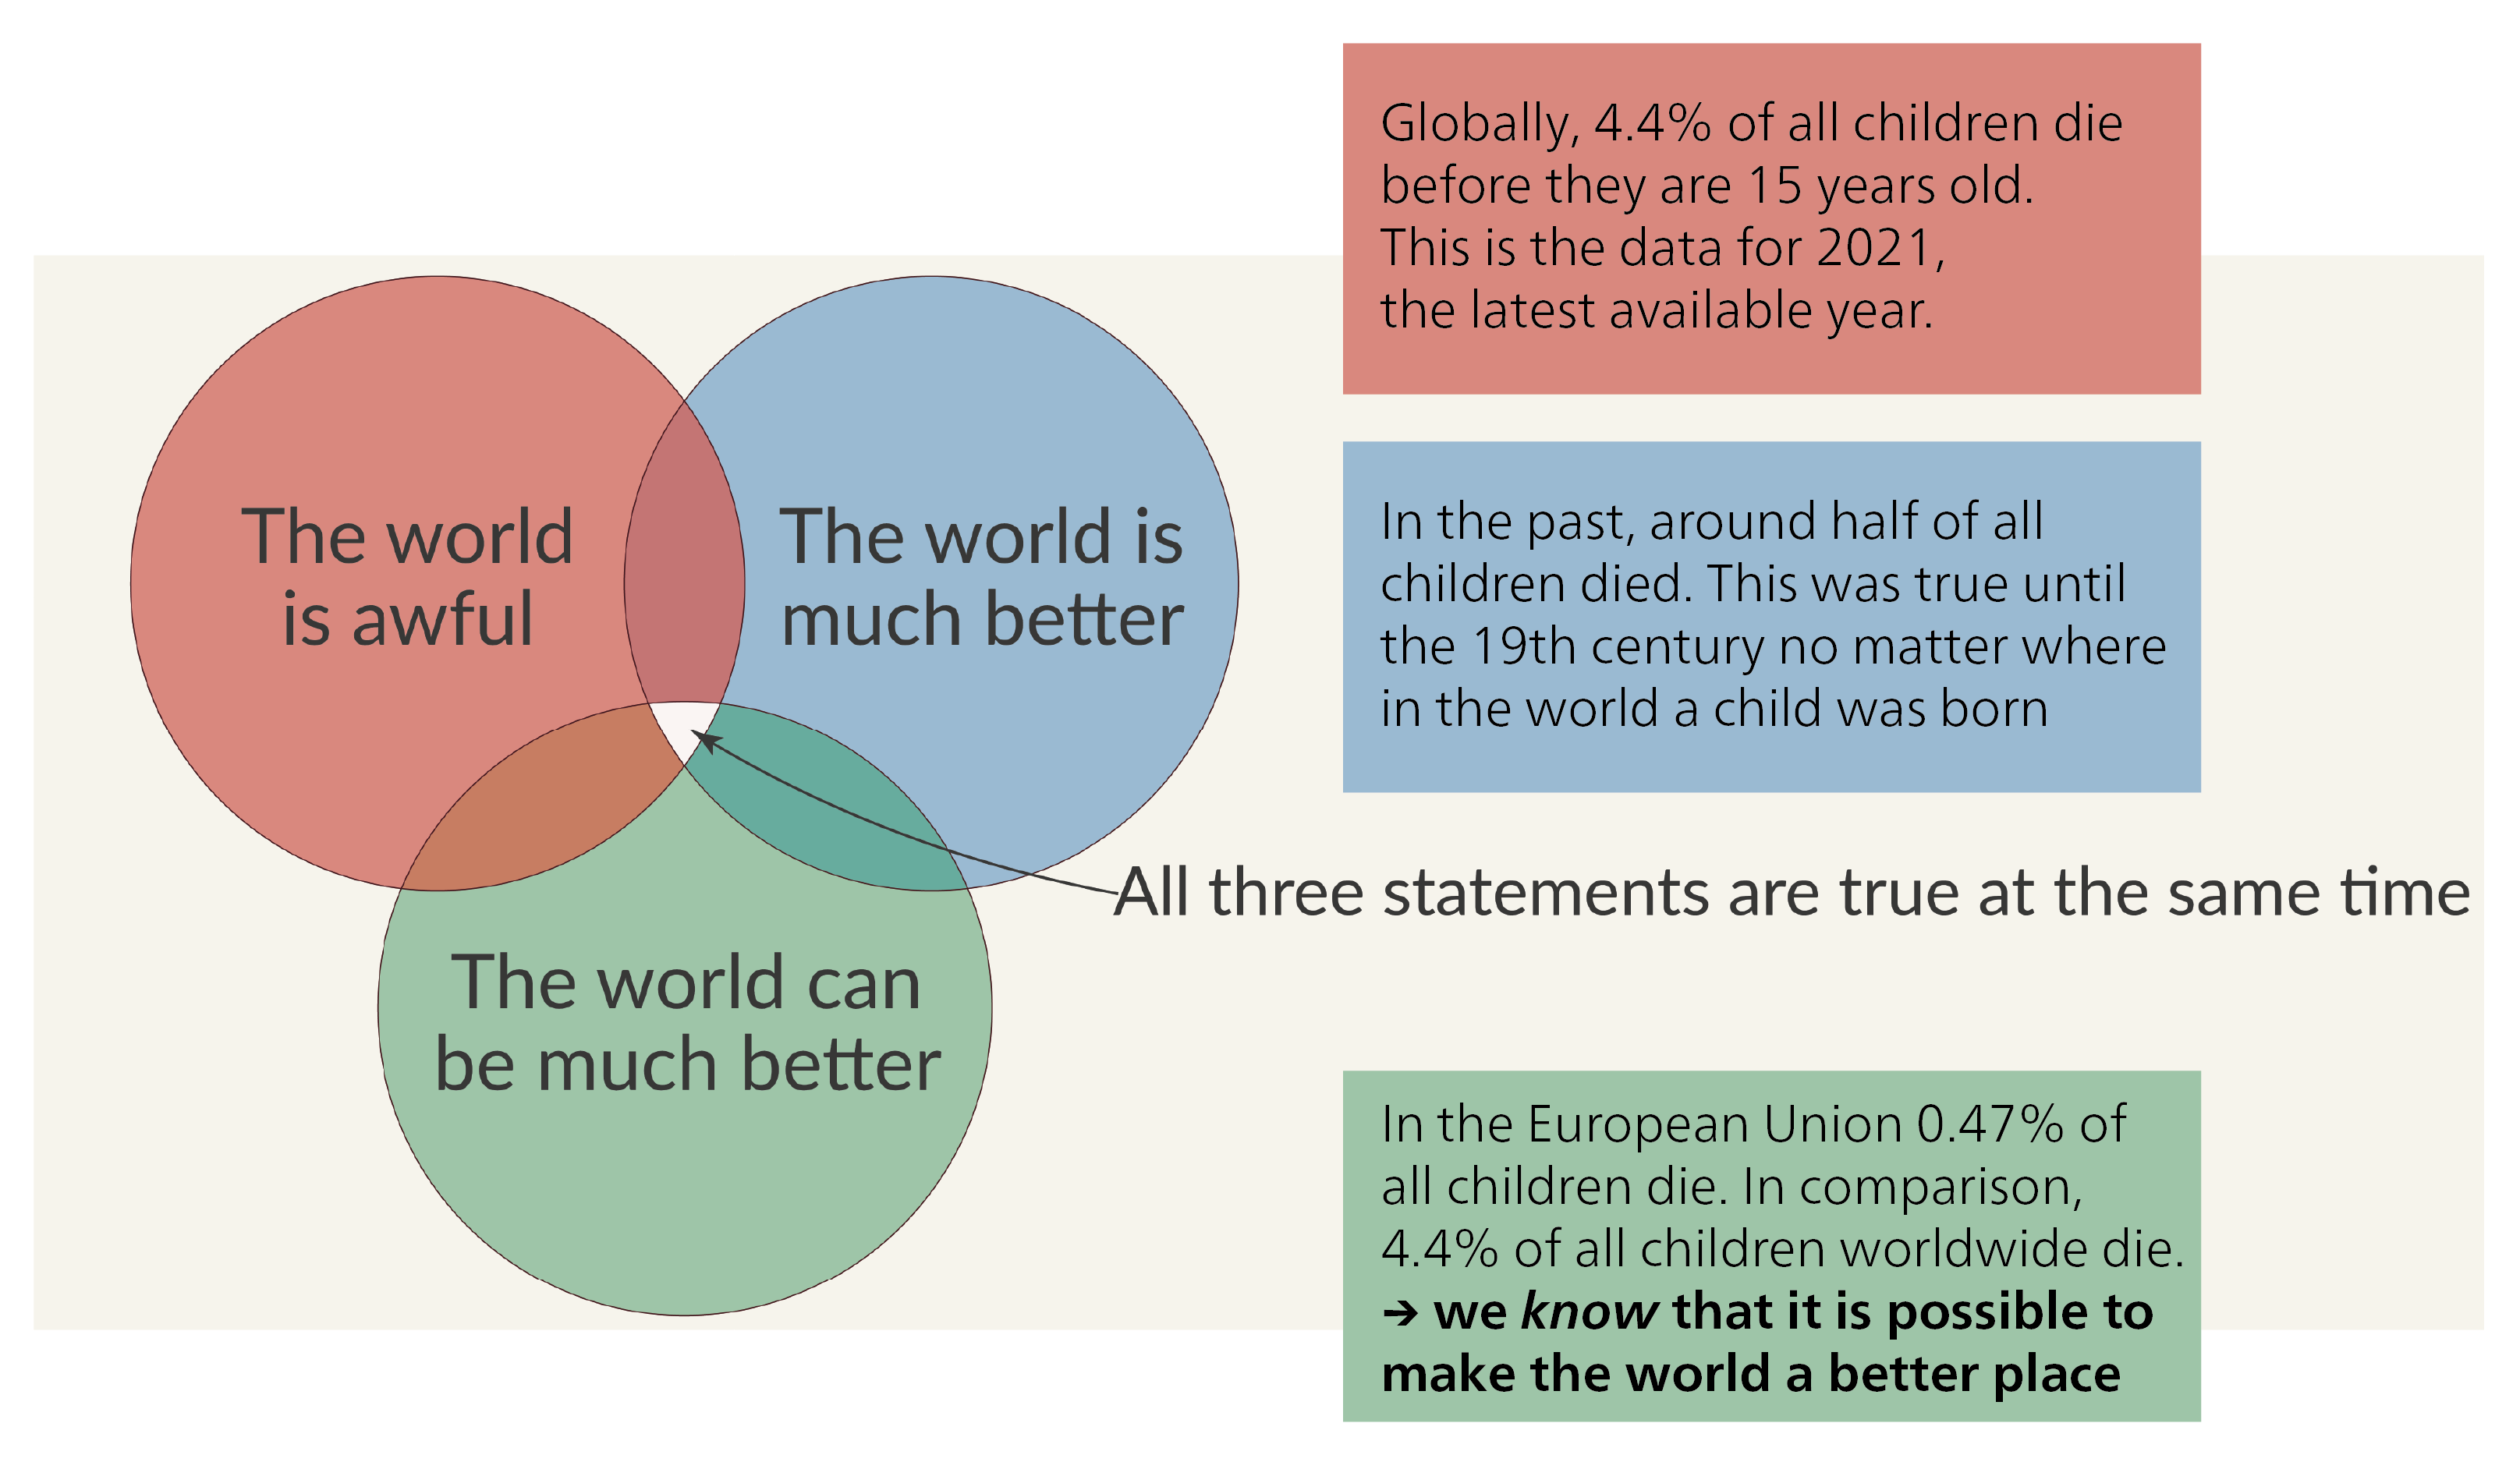
\includegraphics[keepaspectratio]{4_social-sustainability/images/Fig4_11_WorldAwfulBetter.png}}

}

\caption{\label{fig-WordlAwfulBetter}Die Welt ist schrecklich. Die Welt
ist viel besser. Die Welt kann viel besser sein. Alle drei Aussagen sind
gleichzeitig wahr. Quelle: Adaptiert nach Roser (2022),
https://ourworldindata.org/much-better-awful-can-be-better.}

\end{figure}%

Wie Abbildung~\ref{fig-WordlAwfulBetter} zeigt, können drei scheinbar
widersprüchliche Aussagen gleichzeitig wahr sein: In vielerlei Hinsicht
ist die Welt schrecklich. Dennoch ist sie viel besser geworden. Und
schliesslich -- sie kann noch viel besser sein. Diese Perspektive bietet
auch eine gute Grundlage für das Verständnis von Strategien zur sozialen
Nachhaltigkeit.

\begin{enumerate}
\def\labelenumi{\arabic{enumi}.}
\item
  \textbf{„Die Welt ist schrecklich'': Soziale Missstände bestehen.}\\
  Millionen von Menschen weltweit sind von Armut, Hunger,
  Diskriminierung und mangelnder Teilhabe betroffen. Ungleichheiten
  zwischen und innerhalb von Gesellschaften gefährden Zusammenhalt,
  Resilienz und Gerechtigkeit. Strategien für soziale Nachhaltigkeit
  müssen diese Probleme klar benennen und angehen.
\item
  \textbf{„Die Welt ist viel besser'': Fortschritte wurden erzielt.}\\
  Historische Vergleiche zeigen, dass zentrale soziale Indikatoren
  verbessert wurden: geringere Kindersterblichkeit, höhere
  Alphabetisierungsraten, wachsende soziale Rechte. Diese Entwicklungen
  belegen, dass politisches Handeln, soziale Bewegungen und
  institutionelle Reformen wirken. Strategien für soziale Nachhaltigkeit
  können auf diesen Erfolgen aufbauen.
\item
  \textbf{„Die Welt kann viel besser sein'': Das Potenzial ist enorm.}\\
  Inklusion, sozialer Zusammenhalt, Resilienz und
  Verfahrensgerechtigkeit sind die zentralen Hebel zur Überwindung
  bestehender Missstände. Strategien reichen von der Bekämpfung von
  Diskriminierung, dem Ausbau sozialer Sicherungssysteme und der
  Einführung partizipativer Governance bis hin zur Förderung von
  Bildung, Gesundheit und kultureller Vielfalt.
\end{enumerate}

Diese Perspektive zeigt, dass Strategien für soziale Nachhaltigkeit
Missstände klar benennen, auf erzielten Fortschritten aufbauen und neue
Möglichkeiten für mehr Gerechtigkeit schaffen müssen.

Die Herausforderungen sind tatsächlich enorm. Aber wir sind nicht zum
Scheitern verurteilt. Der bereits erzielte Fortschritt zeigt, dass
Wandel möglich ist. Der Schlüssel liegt nun darin, schnell und in
grossem Massstab zu handeln. Wie Hannah Ritchie (2024) feststellt,
verschwenden wir oft Energie bei internen Konflikten unter
Nachhaltigkeitsbefürworter*innen und nutzen damit Gegner*innen der
Sache. Wir brauchen systemischen Wandel und eine melioristische Ethik --
eine Überzeugung, dass die Welt durch bewusstes Handeln Schritt für
Schritt verbessert werden kann. Statt uns in internen
Meinungsverschiedenheiten zu verlieren, brauchen wir gemeinsame
Anstrengungen in dieselbe Richtung -- auch wenn unsere Wege und
Prioritäten variieren.

Am Ende ist es jedoch wichtig zu bedenken, dass Strategien für soziale
Nachhaltigkeit immer einer Diskussion bedürfen. Wer definiert die
Grenzen von Bedürfnissen und Wünschen, wessen Zukunftsvision
nachhaltiger Entwicklung soll verfolgt werden, welche
Nachhaltigkeitspfade bevorzugt werden und wer trifft diese
Entscheidungen? Auch: Wer profitiert vom gewählten Kurs, wer trägt die
Kosten, und welche Verteilungsmuster entstehen daraus? Gerade der
Unterschied zwischen Bedürfnissen und Wünschen zeigt, wie komplex solche
Diskussionen sind: Bedürfnisse sind endlich, universell und
unentbehrlich für das menschliche Wohlergehen, wie Wohnraum oder
Nahrung. Wünsche hingegen sind potenziell unbegrenzt, subjektiv und
entbehrlich, wie die Wahl einer bestimmten Schuhmarke. Wie die Schweizer
Politikerin Jaqueline Badran in einem Interview sagte: „Man kann nicht
kein Zuhause haben. Das ist anders als bei Turnschuhen, wo man sagen
kann: Adidas ist zu teuer für mich, also kaufe ich eine andere Marke.
Das kann man bei Wohnraum nicht tun.'' (Albrecht 2023). Dieses Beispiel
zeigt, dass die Debatte über soziale Nachhaltigkeit nicht nur um
abstrakte Prinzipien geht; es geht um die konkreten, existenziellen
Fragen des Lebens.

Solche Fragen können nicht technokratisch beantwortet werden.
Stattdessen erfordern sie offene, faire und inklusive
Aushandlungsprozesse. Strategien für soziale Nachhaltigkeit müssen daher
nicht nur konkrete Lösungen für Ungerechtigkeiten entwickeln -- sie
müssen auch Räume schaffen, in denen diese Diskussionen geführt werden
können.

\section{Grundlagen der Nachhaltigkeit: Das Quiz -- Kapitel
4}\label{grundlagen-der-nachhaltigkeit-das-quiz-kapitel-4}

Welche der folgenden Aussagen beschreiben die drei Dimensionen der
Gerechtigkeit, die in der sozialen Nachhaltigkeit häufig diskutiert
werden, korrekt? (Mehr als eine Aussage kann richtig sein.)

\begin{itemize}
\tightlist
\item[$\square$]
  Verteilungsgerechtigkeit konzentriert sich auf die faire Verteilung
  von Gütern und Lasten, z. B. den Zugang zu sauberem Wasser oder die
  Belastung durch Umweltverschmutzung.
\item[$\square$]
  Verfahrensgerechtigkeit betont die Inklusivität und Fairness von
  Entscheidungsprozessen und der Repräsentation.
\item[$\square$]
  Verteilungsgerechtigkeit betrifft in erster Linie die Anerkennung
  kultureller Identitäten und historischer Erfahrungen.
\item[$\square$]
  Verfahrensgerechtigkeit befasst sich hauptsächlich mit den Ergebnissen
  von Politiken und nicht damit, wie Entscheidungen getroffen werden.
\item[$\square$]
  Anerkennungsgerechtigkeit konzentriert sich auf den Respekt vor
  sozialen und kulturellen Unterschieden und die Anerkennung
  struktureller Ungerechtigkeiten.
\end{itemize}

In Debatten zur sozialen Nachhaltigkeit befasst sich
Verteilungsgerechtigkeit mit der fairen Verteilung von Vorteilen und
Lasten. Verfahrensgerechtigkeit konzentriert sich darauf, wer in
Entscheidungsprozesse einbezogen wird und wie Entscheidungen getroffen
werden. Anerkennungsgerechtigkeit betont die Bedeutung des Respekts vor
vielfältigen Identitäten, kulturellen Kontexten und historischen
Erfahrungen sowie die Auseinandersetzung mit strukturellen
Ungerechtigkeiten. Die übrigen Aussagen ordnen den Schwerpunkt einer
Gerechtigkeitsdimension fälschlicherweise einer anderen zu.

\begin{itemize}
\tightlist
\item
  True
\item
  True
\item
  False
\item
  False
\item
  True
\end{itemize}

Welche der folgenden Aussagen beschreiben zentrale Dimensionen der
sozialen Nachhaltigkeit korrekt? (Mehr als eine Aussage kann richtig
sein.)

\begin{itemize}
\tightlist
\item[$\square$]
  Resilienz bezeichnet die Fähigkeit einer Gemeinschaft oder
  Gesellschaft, interne oder externe Schocks zu vermeiden, zu
  absorbieren oder zu bewältigen.
\item[$\square$]
  Sozialer Zusammenhalt beschreibt ein gemeinsames Zugehörigkeits- und
  Vertrauensgefühl, das Zusammenarbeit innerhalb von Gemeinschaften
  ermöglicht.
\item[$\square$]
  Sozialer Zusammenhalt wird hauptsächlich durch das Fehlen von Vielfalt
  innerhalb einer Gesellschaft definiert.
\item[$\square$]
  Inklusion konzentriert sich in erster Linie auf Wirtschaftswachstum
  statt auf die Teilhabe am sozialen und politischen Leben.
\item[$\square$]
  Inklusion bezeichnet den Zugang aller Individuen und Gruppen zu
  wirtschaftlichen, politischen, sozialen und kulturellen Bereichen.
\end{itemize}

Inklusion betrifft den gleichberechtigten Zugang und die Teilhabe in
wirtschaftlichen, politischen, sozialen und kulturellen Bereichen.
Sozialer Zusammenhalt betont Vertrauen, Zugehörigkeit und die Fähigkeit
von Gruppen, konstruktiv zusammenzuarbeiten. Resilienz beschreibt die
Fähigkeit von Gesellschaften oder Gemeinschaften, Schocks wie
Umweltveränderungen oder politische Krisen zu bewältigen oder sich an
sie anzupassen. Die übrigen Aussagen stellen diese Konzepte falsch dar,
indem sie ihren Geltungsbereich einschränken oder ihnen unzutreffende
Merkmale zuschreiben.

\begin{itemize}
\tightlist
\item
  True
\item
  True
\item
  False
\item
  False
\item
  True
\end{itemize}

Welche der folgenden Aussagen ist gemäss dem Fähigkeitenansatz korrekt?

\begin{itemize}
\tightlist
\item[$\square$]
  Ressourcen müssen so verteilt werden, dass alle Menschen Zugang zu den
  Fähigkeiten und Zuständen haben, die für ein gutes Leben notwendig
  sind.
\item[$\square$]
  Ressourcen wie sauberes Trinkwasser müssen gleichmässig verteilt
  werden.
\item[$\square$]
  Gleiche Rechtsansprüche reichen aus, damit eine Gesellschaft gerecht
  ist.
\item[$\square$]
  Entwicklung muss anhand des BIP gemessen werden.
\end{itemize}

Der Fähigkeitenansatz fragt danach, was Menschen tatsächlich sein und
tun können. Er betont daher, dass Ressourcen so verteilt werden sollten,
dass alle Individuen die wesentlichen Fähigkeiten und Zustände erreichen
können, die für ein gutes Leben notwendig sind, anstatt sich allein auf
formale Rechte, eine gleichmässige Ressourcenverteilung oder
BIP-Wachstum zu konzentrieren.

\begin{itemize}
\tightlist
\item
  True
\item
  False
\item
  False
\item
  False
\end{itemize}

Welche der folgenden Aussagen unterscheiden individuelle und
strukturelle Ansätze zur Analyse von Ungleichheit korrekt? (Mehr als
eine Aussage kann richtig sein.)

\begin{itemize}
\tightlist
\item[$\square$]
  Analysen individueller Ungleichheit gehen davon aus, dass
  wirtschaftliche Unterschiede hauptsächlich auf persönliche
  Eigenschaften und individuellen Einsatz zurückzuführen sind.
\item[$\square$]
  Analysen struktureller Ungleichheit sind mit Konzepten wie
  Gerechtigkeit, dem Fähigkeitenansatz und relativer Ungleichheit
  verknüpft.
\item[$\square$]
  Analysen individueller Ungleichheit konzentrieren sich auf
  sozioökonomische Merkmale wie Einkommen, Bildung und Berufsstatus.
\item[$\square$]
  Strukturelle Ansätze zur Ungleichheit orientieren sich eng an der
  Wohlfahrtsökonomie und dem Konzept der absoluten Ungleichheit.
\item[$\square$]
  Strukturelle Ungleichheit wird als Ergebnis des sozialen Rahmens
  verstanden, z. B. der Position innerhalb der Produktionsweise,
  sozialer Hierarchien oder der Nationalität.
\end{itemize}

Individuelle Ansätze zur Ungleichheit betonen Unterschiede zwischen
Einzelpersonen und stützen sich typischerweise auf die
Wohlfahrtsökonomie und absolute Ungleichheit, wobei Ungleichheiten
weitgehend auf persönliche Eigenschaften und Einsatz zurückgeführt
werden. Strukturelle Ansätze hingegen konzentrieren sich auf die
sozialen, wirtschaftlichen und politischen Rahmenbedingungen, die
ungleiche Ergebnisse prägen, und sind eng mit Konzepten wie
Gerechtigkeit, dem Fähigkeitenansatz und relativer Ungleichheit
verbunden.

\begin{itemize}
\tightlist
\item
  True
\item
  True
\item
  True
\item
  False
\item
  True
\end{itemize}

Was beschreibt Resilienz im Kontext sozialer Nachhaltigkeit am
treffendsten?

\begin{itemize}
\tightlist
\item[$\square$]
  Der kurzfristige Einsatz von Ressourcen, um das Wirtschaftswachstum
  nach einer Krise zu stabilisieren.
\item[$\square$]
  Die Fähigkeit von Gesellschaften, sämtliche internen und externen
  Schocks vollständig zu vermeiden.
\item[$\square$]
  Die Fähigkeit von Individuen und Gesellschaften, sich auf Schocks
  vorzubereiten, mit ihnen umzugehen und sich von ihnen zu erholen.
\item[$\square$]
  Die gleichmässige Verteilung von Einkommen, um soziale Konflikte zu
  verhindern.
\end{itemize}

Resilienz bezeichnet die Fähigkeit von Individuen, Haushalten,
Gemeinschaften oder ganzen Gesellschaften, sich auf Schocks wie
Wirtschaftskrisen, Naturkatastrophen oder soziale Konflikte
vorzubereiten, mit ihnen umzugehen und sich von ihnen zu erholen. Sie
bedeutet nicht die vollständige Vermeidung von Schocks, sondern die
Fähigkeit, mit ihnen umzugehen und Lebensqualität und Stabilität
wiederzuerlangen.

\begin{itemize}
\tightlist
\item
  False
\item
  False
\item
  True
\item
  False
\end{itemize}

Welche Strategie zum Aufbau von Resilienz konzentriert sich auf
langfristigen systemischen Wandel statt auf unmittelbare Reaktionen auf
Schocks?

\begin{itemize}
\tightlist
\item[$\square$]
  Risikominderung und -reduktion, wie Impfungen oder
  Schutzinfrastruktur.
\item[$\square$]
  Bewältigungsstrategien, wie das Zurückgreifen auf Ersparnisse oder
  soziale Netzwerke.
\item[$\square$]
  Sofortmassnahmen zur Nothilfe unmittelbar nach einer Katastrophe.
\item[$\square$]
  Transformative Strategien, wie institutionelle Reformen und
  Veränderungen sozialer Normen.
\end{itemize}

Transformative Strategien zielen auf eine langfristige Steigerung der
Resilienz ab, indem sie weitreichende Reformen oder neue Institutionen
einführen. Sie kombinieren typischerweise Elemente der Risikominderung
und Bewältigung, gehen aber über kurzfristige Reaktionen hinaus, indem
sie zugrunde liegende Verwundbarkeiten adressieren und soziale,
institutionelle oder strukturelle Bedingungen verändern.

\begin{itemize}
\tightlist
\item
  False
\item
  False
\item
  False
\item
  True
\end{itemize}

Welche der folgenden Aussagen geben korrekt wieder, wie verschiedene
Gerechtigkeitstheorien die Idee eines bedingungslosen Grundeinkommens
beurteilen? (Mehr als eine Aussage kann richtig sein.)

\begin{itemize}
\tightlist
\item[$\square$]
  Kollektive Gerechtigkeitstheorien bewerten ein bedingungsloses
  Grundeinkommen abhängig vom historischen, kulturellen und sozialen
  Kontext.
\item[$\square$]
  Liberale Theorien können ein bedingungsloses Grundeinkommen
  befürworten, da es den Gesamtnutzen steigern oder gleiche
  Grundfreiheiten stärken kann.
\item[$\square$]
  Egalitaristische Perspektiven befürworten ein bedingungsloses
  Grundeinkommen unkritisch, da strikte Gleichheit automatisch
  Gerechtigkeit garantiert.
\item[$\square$]
  Libertäre Theorien lehnen ein bedingungsloses Grundeinkommen im
  Allgemeinen ab, da Umverteilung durch Besteuerung als Eingriff in die
  individuelle Freiheit und Eigentumsrechte gilt.
\item[$\square$]
  Alle Gerechtigkeitstheorien sind sich einig, dass ein bedingungsloses
  Grundeinkommen die gerechteste Form der Umverteilung ist.
\end{itemize}

Verschiedene Gerechtigkeitstheorien kommen zu unterschiedlichen
Schlüssen hinsichtlich eines bedingungslosen Grundeinkommens. Libertäre
Theorien lehnen es typischerweise wegen Bedenken über staatliche
Eingriffe und Eigentumsrechte ab. Liberale Theorien wie der
Utilitarismus oder der Rawls'sche Kontraktarismus können es unter
bestimmten Bedingungen befürworten, während egalitaristische Ansätze
betonen, dass Gleichheit von Fairness unterschieden werden muss.
Kollektive Theorien betonen, dass Urteile vom sozialen und kulturellen
Kontext abhängen. Es besteht kein universeller Konsens unter allen
Theorien.

\begin{itemize}
\tightlist
\item
  True
\item
  True
\item
  False
\item
  True
\item
  False
\end{itemize}

\chapter{Wirtschaftliche
Nachhaltigkeit}\label{wirtschaftliche-nachhaltigkeit}

\begin{figure}[H]

\centering{

\pandocbounded{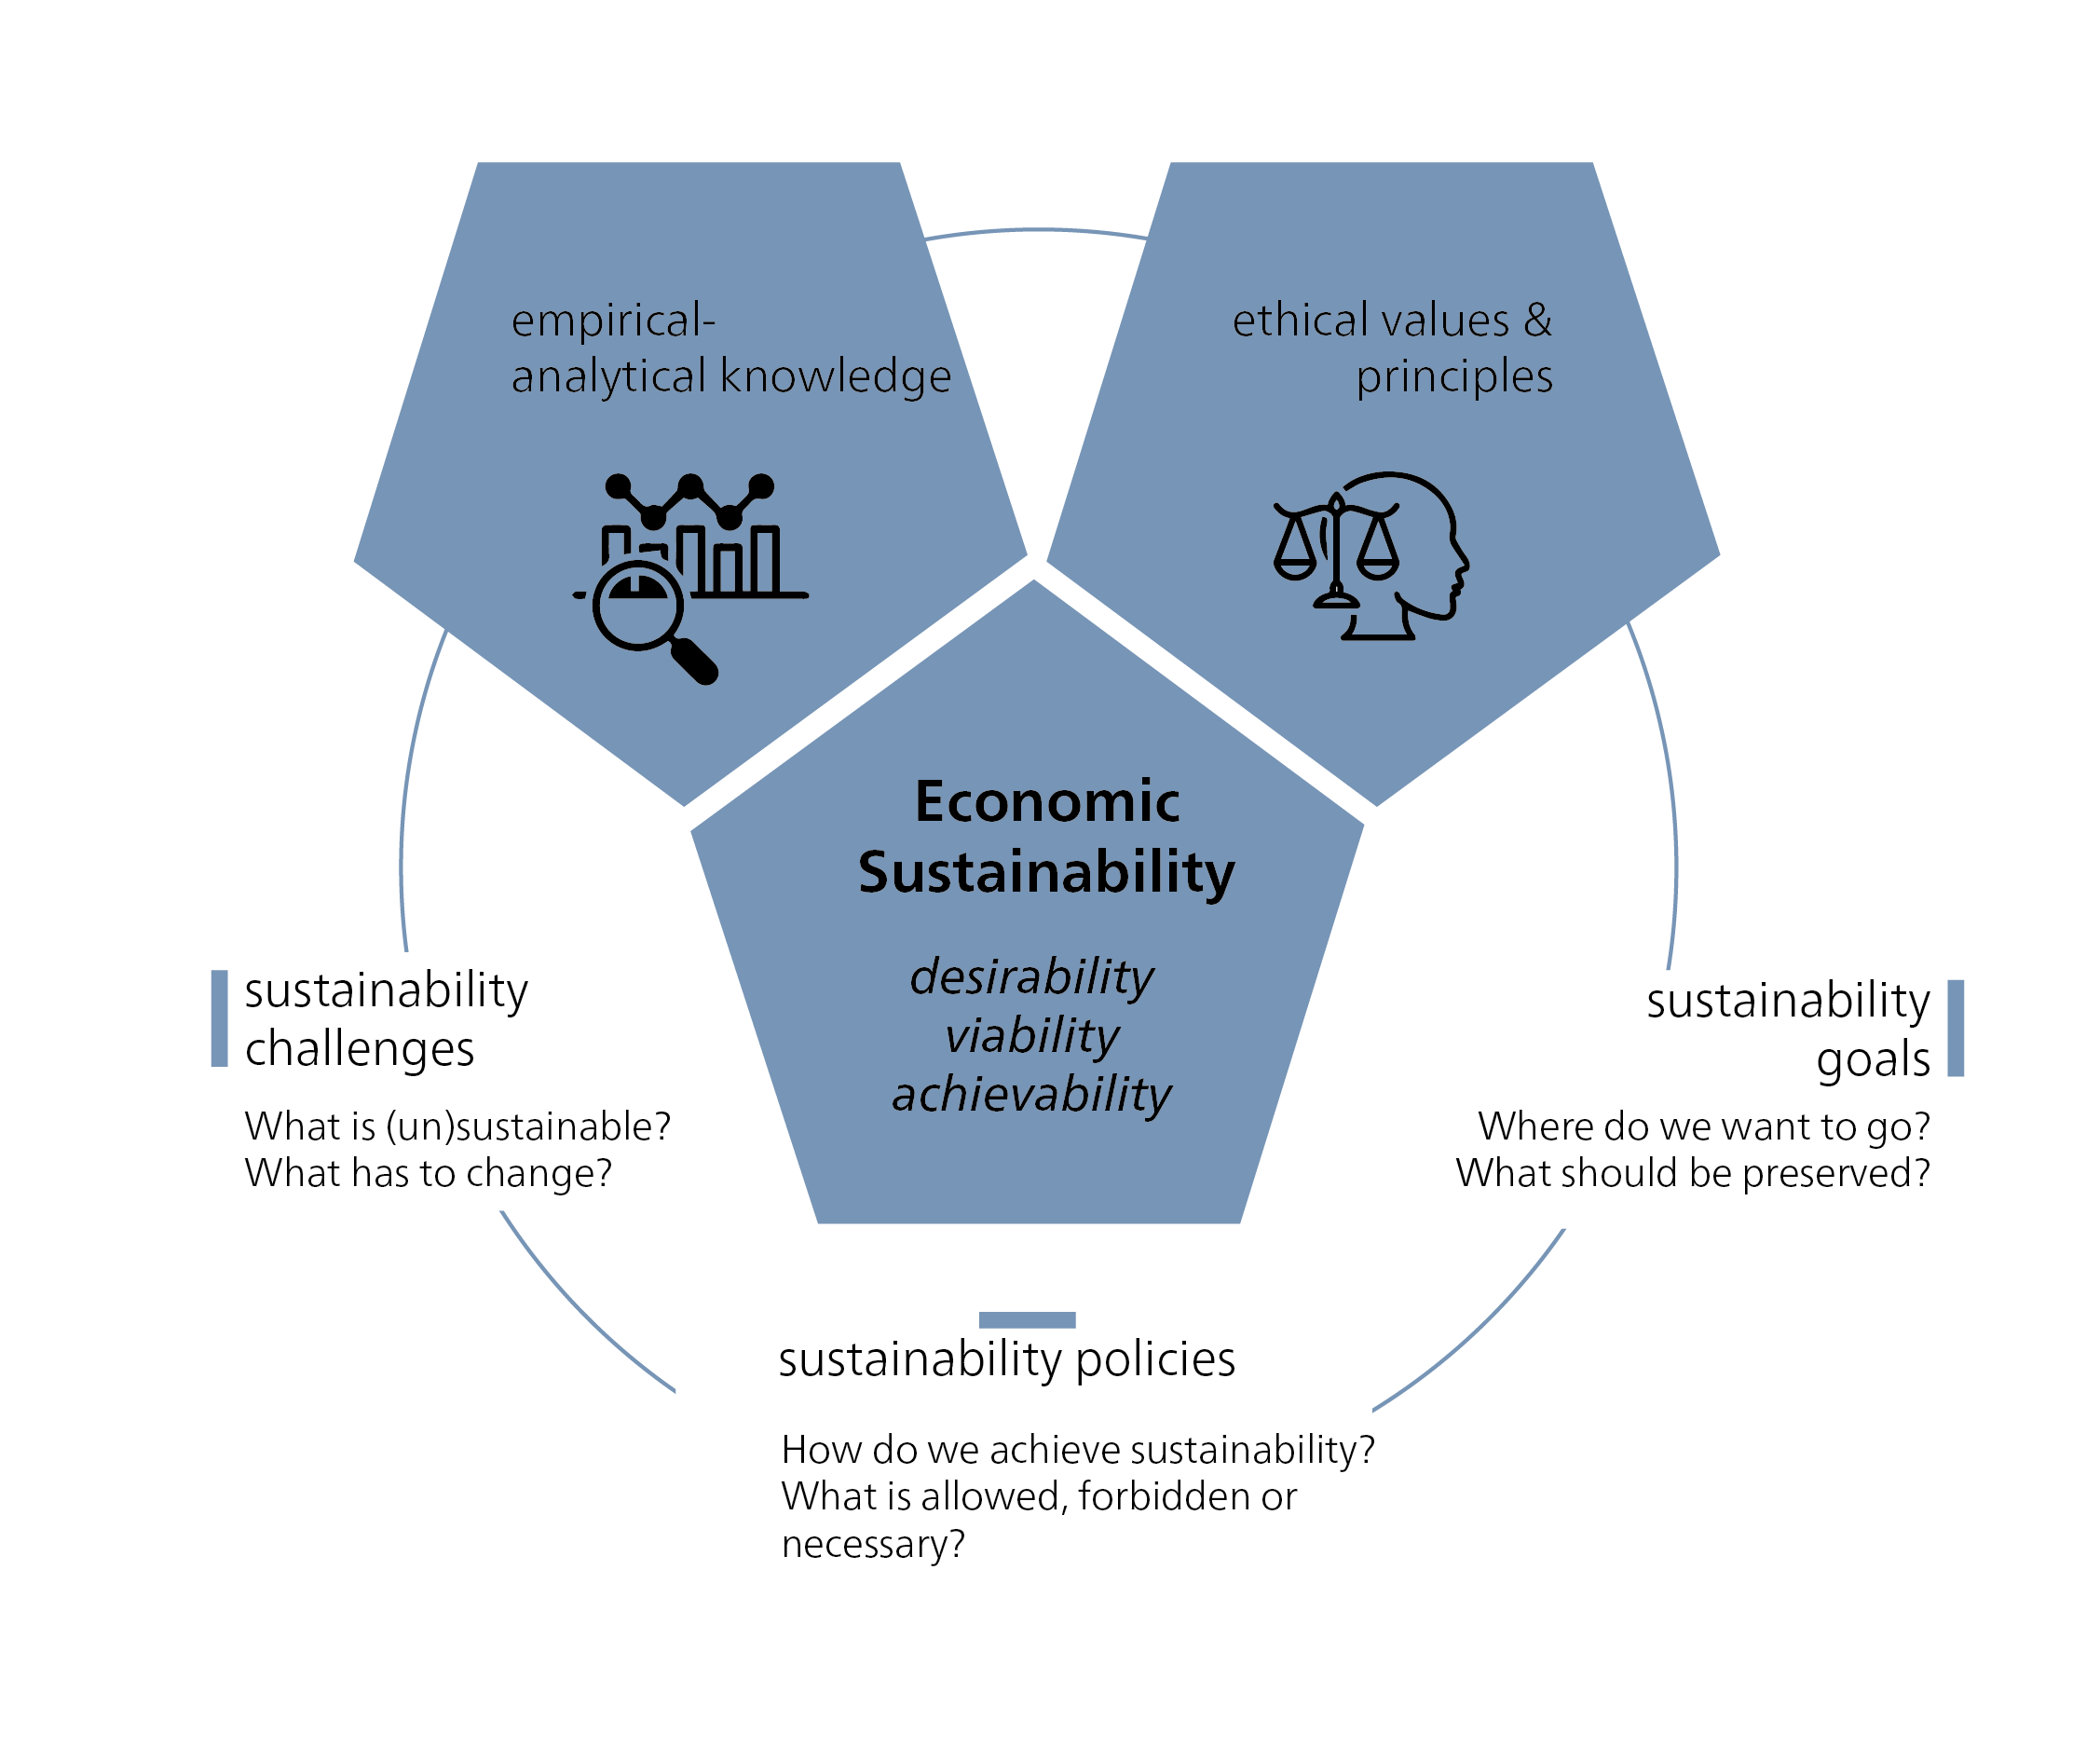
\includegraphics[keepaspectratio]{5_economic-sustainability/images/Fig5_1_NEeconomic.png}}

}

\caption{\label{fig-ne-econ}Wirtschaftliche Nachhaltigkeit. Quelle:
Eigene Darstellung.}

\end{figure}%

Wirtschaftliche Nachhaltigkeit ist ein zutiefst normatives Konzept: Es
fragt, welches Wirtschaftsverständnis gesellschaftlich wünschenswert
ist, welche Ziele wirtschaftliche Aktivitäten verfolgen sollten und
welche Rolle Menschen, Gesellschaft und natürliche Ressourcen dabei
spielen sollten. Entgegen weitverbreiteter Überzeugung sind
Wirtschaftstheorien nicht wertneutral. Stattdessen sind sie normativ und
performativ und formen Ideen, Handlungen, Politiken und -- letztlich --
die Wirklichkeit. Deshalb unterscheiden sich die Antworten auf die
zentralen Fragen der Wirtschaft -- d.~h. wer produziert und konsumiert
was und warum, wie werden Gewinne verteilt und wofür werden sie
verwendet -- je nach Wirtschaftstheorie.

\begin{tcolorbox}[enhanced jigsaw, arc=.35mm, bottomrule=.15mm, bottomtitle=1mm, breakable, colback=white, colbacktitle=quarto-callout-note-color!10!white, colframe=quarto-callout-note-color-frame, coltitle=black, left=2mm, leftrule=.75mm, opacityback=0, opacitybacktitle=0.6, rightrule=.15mm, title={Definition von Rente, Gewinn und Lohn}, titlerule=0mm, toprule=.15mm, toptitle=1mm]

\begin{quote}
„Der Ertrag der Erde -- alles, was durch die vereinte Anwendung von
Arbeit, Maschinen und Kapital aus ihrer Oberfläche gewonnen wird, wird
unter drei Klassen der Gesellschaft aufgeteilt, nämlich den Eigentümer
des Landes \textbf{{[}Rente{]}}, den Eigentümer des Vorrats oder
Kapitals \textbf{{[}Gewinn{]}}, das für seine Bewirtschaftung notwendig
ist, und die Arbeiter, durch deren Fleiss es bewirtschaftet wird
\textbf{{[}Lohn{]}}. \ldots Die Gesetze zu bestimmen, die diese
Verteilung regeln, ist das Hauptproblem der Politischen Ökonomie.''\\
Vorwort, S. 1 -- David Ricardo: The Principles of Political Economy and
Taxation (1821)
\end{quote}

\end{tcolorbox}

\section{Wirtschaft als performative
Wissenschaft}\label{wirtschaft-als-performative-wissenschaft}

Von Anfang an hat die moderne Wirtschaftswissenschaft die soziale
Wirklichkeit nicht nur beobachtet und beschrieben -- sie hat sie auch
mitgestaltet. Diese Disziplin hat unser Denken darüber geprägt, was als
„wirtschaftlich'' gilt -- z. B. durch das Ideal des rational
entscheidenden Homo oeconomicus, die Norm der Gewinnmaximierung, den
Fokus auf Effizienz oder die Idee, dass Wachstum mit sozialem
Fortschritt gleichzusetzen ist (vgl. Bontrup und Marquardt 2021, 1--40).

Diese Interpretationen blieben nie rein theoretisch. Sie beeinflussen
Politik und Praxis bis heute: vom Strukturwandel bis zur
Marktliberalisierung, die sich in den 1980er Jahren durchsetzte -- bis
hin zur Gestaltung der Klimapolitik durch Emissionshandelssysteme und
der Konstruktion hochkomplexer Finanzprodukte. Die Geschichte der
Wirtschaftswissenschaft ist daher auch eine Geschichte ihrer Wirkung
(Schneidewind et al.~2016). Die am weitesten verbreitete Definition der
Wirtschaftswissenschaft, ursprünglich von Lionel Robbins geprägt,
konzentriert sich auf das Verhältnis zwischen Ressourcenknappheit und
der Befriedigung menschlicher Bedürfnisse:

\begin{quote}
„Wirtschaft ist die Wissenschaft, die menschliches Verhalten als
Beziehung zwischen Zwecken und knappen Mitteln, die alternative
Verwendungsmöglichkeiten haben, untersucht.'' (Robbins 1932, p.~15).
\end{quote}

Robbins' Definition ist von seiner theoretischen Ausrichtung auf die
neoklassische Wirtschaft beeinflusst, die Denkschule, die als
Mainstream-Ökonomie gilt. Die meisten Lehrbücher definieren
Wirtschaftswissenschaft in Erweiterung dieses Konzepts als Wissenschaft
der (rationalen) Entscheidungsfindung, die untersucht, wie Menschen
entscheiden, knappe Ressourcen zur Erreichung ihrer Ziele einzusetzen.

\begin{tcolorbox}[enhanced jigsaw, arc=.35mm, bottomrule=.15mm, bottomtitle=1mm, breakable, colback=white, colbacktitle=quarto-callout-note-color!10!white, colframe=quarto-callout-note-color-frame, coltitle=black, left=2mm, leftrule=.75mm, opacityback=0, opacitybacktitle=0.6, rightrule=.15mm, title={Homo oeconomicus als grundlegendes Modell menschlichen Verhaltens}, titlerule=0mm, toprule=.15mm, toptitle=1mm]

\emph{Homo oeconomicus}, oder „Wirtschaftsmensch'', ist ein
grundlegendes Modell in der neoklassischen Wirtschaft. Es beschreibt
Menschen als rationale, nutzenmaximierende Akteure, die Zugang zu
umfassenden Informationen haben und konsequent Entscheidungen treffen,
um ihr materielles Wohlergehen zu steigern. Diese Sichtweise des
Menschen war entscheidend für die Entwicklung mathematischer Modelle in
der Wirtschaft und die Idee, dass Märkte effizient zu optimalen
Ergebnissen führen können.

Historisch entwickelte sich dieses Konzept über mehrere Stufen. Während
frühe Wirtschaftswissenschaftler wie Adam Smith noch ein komplexeres
Menschenbild annahmen -- eines, das auch moralische und soziale
Dimensionen einschloss --, wurde dieses in der Marginalrevolution des
19. Jahrhunderts zunehmend auf rein rationales, kalkulierendes Verhalten
reduziert. Diese Reduktion ermöglichte es, wirtschaftliche Prozesse
mathematisch zu modellieren, führte jedoch auch zu einer problematischen
Abstraktion von tatsächlichen sozialen, ökologischen und psychologischen
Bedingungen.

Kritiker*innen betonen, dass \emph{Homo oeconomicus} ein normatives und
kein rein analytisches Konstrukt ist. Es vermittelt eine spezifische
Vorstellung vom Menschen, wie er in sozialen Modellen und Institutionen
dargestellt wird, die Wettbewerb, Eigenverantwortung und gesteigerte
Effizienz als natürliche Prinzipien betrachtet. In der realen Welt
verhalten sich Menschen jedoch oft nicht rein rational. Stattdessen
prägen Faktoren wie Kooperation, Fairness, Vertrauen und sogar kognitive
Verzerrungen ihre Entscheidungen.

Das \emph{Homo oeconomicus}-Modell ist besonders relevant für die
Diskussion über nachhaltige Entwicklung. Es trägt dazu bei, die
systemischen Ursachen von Umweltzerstörung und sozialer Ungleichheit zu
verschleiern, da es strukturelle Machtverhältnisse, externe Effekte und
langfristige planetare Grenzen systematisch ignoriert.

\end{tcolorbox}

Der heterodoxe Wirtschaftswissenschaftler Ha-Joon Chang kritisiert
Robbins' Definition als zu spezifisch und als aus einem theoretischen
Ansatz hervorgehend, was dazu führt, dass sie in der Folge eine
bestimmte Richtung vorschreibt (Chang 2014). Chang definiert Wirtschaft
nicht durch einen theoretischen Ansatz, sondern durch seinen
Untersuchungsgegenstand: die Wirtschaft. Wirtschaftswissenschaft ist
daher die Lehre von allem, was mit der (Re-)Produktion, dem Austausch
und der Verteilung von Gütern und Dienstleistungen zur Befriedigung
menschlicher Bedürfnisse zusammenhängt. Es gibt natürlich viele andere
Definitionen der Wirtschaftswissenschaft. Aufbauend auf diesen
vielfältigen Verständnissen unterscheiden sich verschiedene Denkschulen
folglich in ihrem Studienschwerpunkt, der Machtstrukturen, Institutionen
oder makroökonomische und soziale Zusammenhänge und Strukturen umfassen
kann (vgl. Miyamura 2020; Newman 2025).

Wirtschaftliche Nachhaltigkeit erfordert, dass wir die Folgen
wirtschaftlicher Aktivitäten für Mensch und Natur systematisch
berücksichtigen. Dazu gehört auch das Stellen von Fragen zur Verteilung.
Wer trägt die Kosten des Wachstums, und wer profitiert davon? Wie viel
materielle Anhäufung ist genug? Und wer entscheidet?

Ein Nachhaltigkeitsverständnis, das diese Fragen ernst nimmt,
konzentriert sich auf Konzepte wie Suffizienz, soziale Mindeststandards
und planetare Grenzen. Es erfordert eine Abkehr vom Dogma einer
wachstumsorientierten Ausrichtung (die Wachstum hauptsächlich am
Bruttoinlandsprodukt misst, vgl. \emph{Kapitel 5.2.3 zu
Wirtschaftswachstum}) hin zu einer normativ begründeten, reflexiven und
pluralistischen Wirtschaft. Eine solche Ausrichtung kann nicht allein
durch die Wirtschaftswissenschaft erreicht werden -- sie muss als
demokratische Praxis im Dialog mit Ethik, anderen Sozialwissenschaften
und Umweltwissenschaften entstehen.

\begin{tcolorbox}[enhanced jigsaw, arc=.35mm, bottomrule=.15mm, bottomtitle=1mm, breakable, colback=white, colbacktitle=quarto-callout-note-color!10!white, colframe=quarto-callout-note-color-frame, coltitle=black, left=2mm, leftrule=.75mm, opacityback=0, opacitybacktitle=0.6, rightrule=.15mm, title={Plurale Ökonomik}, titlerule=0mm, toprule=.15mm, toptitle=1mm]

Die zeitgenössische Wirtschaftswissenschaft wird weitgehend von einer
Denkschule dominiert: der neoklassischen Wirtschaft. An den meisten
Universitäten und in den meisten Kontexten bezeichnet der Begriff
„Wirtschaftswissenschaft'' implizit diese Denkschule. Neoklassische
Wirtschaft bildet den Kern der Mainstream-Ökonomie, basierend auf dem
von Lionel Robbins formulierten Wirtschaftsverständnis. Dementsprechend
untersucht diese Denkschule die Allokation knapper Ressourcen und Güter
auf der Grundlage von Entscheidungen rational handelnder,
nutzenmaximierender Individuen. Der Preismechanismus dient als zentrales
Allokationsinstrument. Angebot und Nachfrage bestimmen den optimalen
Marktpreis, der dann eine optimale Allokation von Ressourcen und Gütern
gewährleistet.

Plurale Ökonomik betont, dass es nicht „die eine''
Wirtschaftswissenschaft gibt, sondern eine Vielzahl von Denkschulen.
Dazu gehören feministische, postkeynesianische, ökologische oder
marxistische Wirtschaft, die sich alle in ihren theoretischen Annahmen,
Methoden und Zielen unterscheiden. Folglich kommen sie oft zu
unterschiedlichen, manchmal komplementären und manchmal
widersprüchlichen Schlussfolgerungen.

Dabei geht es jedoch nicht um eine pauschale Ablehnung der
neoklassischen Wirtschaft. Stattdessen liegt der Schlüssel darin, zu
erkennen, welche Perspektive für eine gegebene Frage am besten geeignet
ist. Neoklassische Analyse bietet nützliche Einblicke in Märkte,
Preisbildung und Anreizstrukturen. Ihr Nutzen ist jedoch begrenzt, wenn
es um nicht-monetäre Prozesse, Machtverhältnisse oder soziale
Reproduktionsarbeit geht. Ihr Fokus auf marktbasierte
Austauschbeziehungen und Preismechanismen macht es beispielsweise
schwierig, unbezahlte Arbeit zu berücksichtigen. Hier setzen alternative
Ansätze wie die feministische Wirtschaft an, die Pflegearbeit, soziale
Beziehungen und Machtstrukturen systematisch in die Wirtschaftsanalyse
einbeziehen. Folglich befürwortet plurale Ökonomik einen methodisch
offenen, problemorientierten Ansatz und betrachtet die Vielfalt
theoretischer Ansätze als Bereicherung -- insbesondere angesichts der
komplexen Herausforderungen nachhaltiger Entwicklung.

Eine detaillierte Auseinandersetzung mit neoklassischer Wirtschaft und
anderen Denkschulen würde den Rahmen dieser Diskussion sprengen. Tiefer
in dieses Thema einsteigen können Sie in unserem Kurs
\href{https://cdeteaching.github.io/SP_SustainableEconomics/}{\emph{Einführung
in die nachhaltige Wirtschaft}}. Weitere Informationen zur pluralen
Ökonomik finden Sie auch auf der E-Learning-Plattform
\href{https://www.exploring-economics.org/en/}{\emph{Exploring
Economics}}.

In diesem Video -- \emph{Economics is for Everyone} -- gibt Ha-Joon
Chang eine klare und prägnante Einführung in die Idee der pluralen
Ökonomik. Er erklärt, warum wirtschaftliches Denken nie neutral ist --
und warum wir dringend mehr wirtschaftlichen Pluralismus brauchen.



\end{tcolorbox}

\section{Schlüsselelemente wirtschaftlicher
Nachhaltigkeit}\label{schluxfcsselelemente-wirtschaftlicher-nachhaltigkeit}

Nachhaltigkeit in der wirtschaftlichen Dimension bedeutet,
wirtschaftliche Aktivitäten so zu gestalten, dass menschliche
Bedürfnisse langfristig -- für gegenwärtige und künftige Generationen --
erfüllt werden, während planetare Grenzen respektiert und faire soziale
Strukturen aufrechterhalten werden. Wirtschaftliche Aktivitäten sind
Prozesse, die natürliche Ressourcen mithilfe zusätzlicher
Produktionsfaktoren wie Arbeit und Kapital in Güter und Dienstleistungen
zum Konsum umwandeln.

In der Wirtschaftstheorie stellt das Ergebnis der Produktion einen
\emph{Wert} dar. Aber welches Wertverständnis liegt dieser Annahme
zugrunde? Historisch gesehen hat das Konzept des Werts in der
Wirtschaftswissenschaft mehrere grundlegende Wandlungen durchlaufen
(vgl. Mazzucato 2018). Bereits im 17. Jahrhundert wurde wirtschaftliche
Aktivität oft als dem Gemeinwohl dienend verstanden, insbesondere wenn
sie zur Versorgungssicherheit oder sozialen Stabilität beitrug. Dieses
Verständnis war eng mit der Idee einer „moralischen Ökonomie'' verknüpft
(vgl. Thompson 1971), die wirtschaftliche Aktivität als eingebettet in
traditionelle Normen, Gerechtigkeitserwartungen und soziale
Verpflichtungen betrachtete.

Der Aufstieg des Kaufmannskapitalismus und die koloniale Expansion
verschoben den Fokus der wirtschaftlichen Wertattribution. In dieser
Zeit wurde Reichtum zunehmend durch Gold, Silber und andere Edelmetalle
verkörpert. Befürworter*innen „merkantilistischer'' Politiken -- ein
Begriff, der nachträglich geprägt wurde, um die vorherrschenden
wirtschaftlichen Praktiken des 16. bis 18. Jahrhunderts zu beschreiben
-- betrachteten Handel als die Hauptquelle nationalen Wohlstands.
Händler und Kaufleute galten daher als „produktiv'', während
Arbeiter*innen und Soldaten als „unproduktiv'' eingestuft wurden.

Die Industrielle Revolution im 18. und 19. Jahrhundert in
Grossbritannien veränderte das wirtschaftliche Wertverständnis erneut
grundlegend: Nun galt \emph{Arbeit} als die Hauptquelle der
Wertschöpfung. Klassische Wirtschaftswissenschaftler wie Adam Smith,
David Ricardo und Karl Marx vertraten eine objektive Werttheorie und
behaupteten, dass der Wert eines Gutes grundlegend durch die in seiner
Produktion investierte Arbeit bestimmt wird. Diese Denker unterschieden
zwischen zwei Schlüsselkonzepten: Gebrauchswert (der praktische Nutzen
eines Gutes) und Tauschwert (der Wert, den ein Gut beim Austausch auf
dem Markt erzielt). Während der Gebrauchswert mit der Befriedigung von
Bedürfnissen zusammenhängt, galt nur Arbeit als Quelle wirtschaftlichen
Wertes. Adam Smith hob insbesondere die Arbeitsteilung als
Schlüsselfaktor des wirtschaftlichen Fortschritts hervor: Er
argumentierte, dass Spezialisierung und die funktionale Aufgliederung
von Produktionsprozessen es ermöglichten, mit der gleichen Menge Arbeit
deutlich mehr Output zu erzielen. Dies wiederum förderte Produktivität,
Innovation und letztlich Wirtschaftswachstum -- Dynamiken, die durch
Mechanisierung und technologische Innovationen weiter verstärkt wurden.

Im späten 19. Jahrhundert entstand dann ein weiteres Verständnis: die
subjektive Werttheorie, die besagt, dass der Wert eines Gutes aus dem
individuellen Nutzen abgeleitet wird, den Konsument*innen ihm
zuschreiben -- unabhängig von Produktionskosten oder Arbeitsstunden.
Diese Sichtweise prägt die neoklassische Wirtschaft bis heute, die
wirtschaftliche Prozesse als rationale Austausche zwischen
Produzent*innen und Konsument*innen modelliert.

Dies ist auch die Grundlage für den einfachen Wirtschaftskreislauf, der
die komplexen Prozesse einer Wirtschaft auf zwei Hauptakteure --
Haushalte und Unternehmen -- und zwei Hauptflüsse --
Güter/Dienstleistungen und Geld -- reduziert. Haushalte stellen
Unternehmen ihre Arbeit im Austausch gegen Einkommen zur Verfügung;
Unternehmen nutzen wiederum diese Arbeit und andere Produktionsfaktoren,
um Güter und Dienstleistungen zu produzieren, die dann von Haushalten
konsumiert werden. Erweiterte Wirtschaftskreisläufe umfassen weitere
Akteure wie Staat, Banken und Aussenhandel.

\begin{figure}

\begin{minipage}[t]{0.50\linewidth}

\begin{figure}[H]

\centering{

\pandocbounded{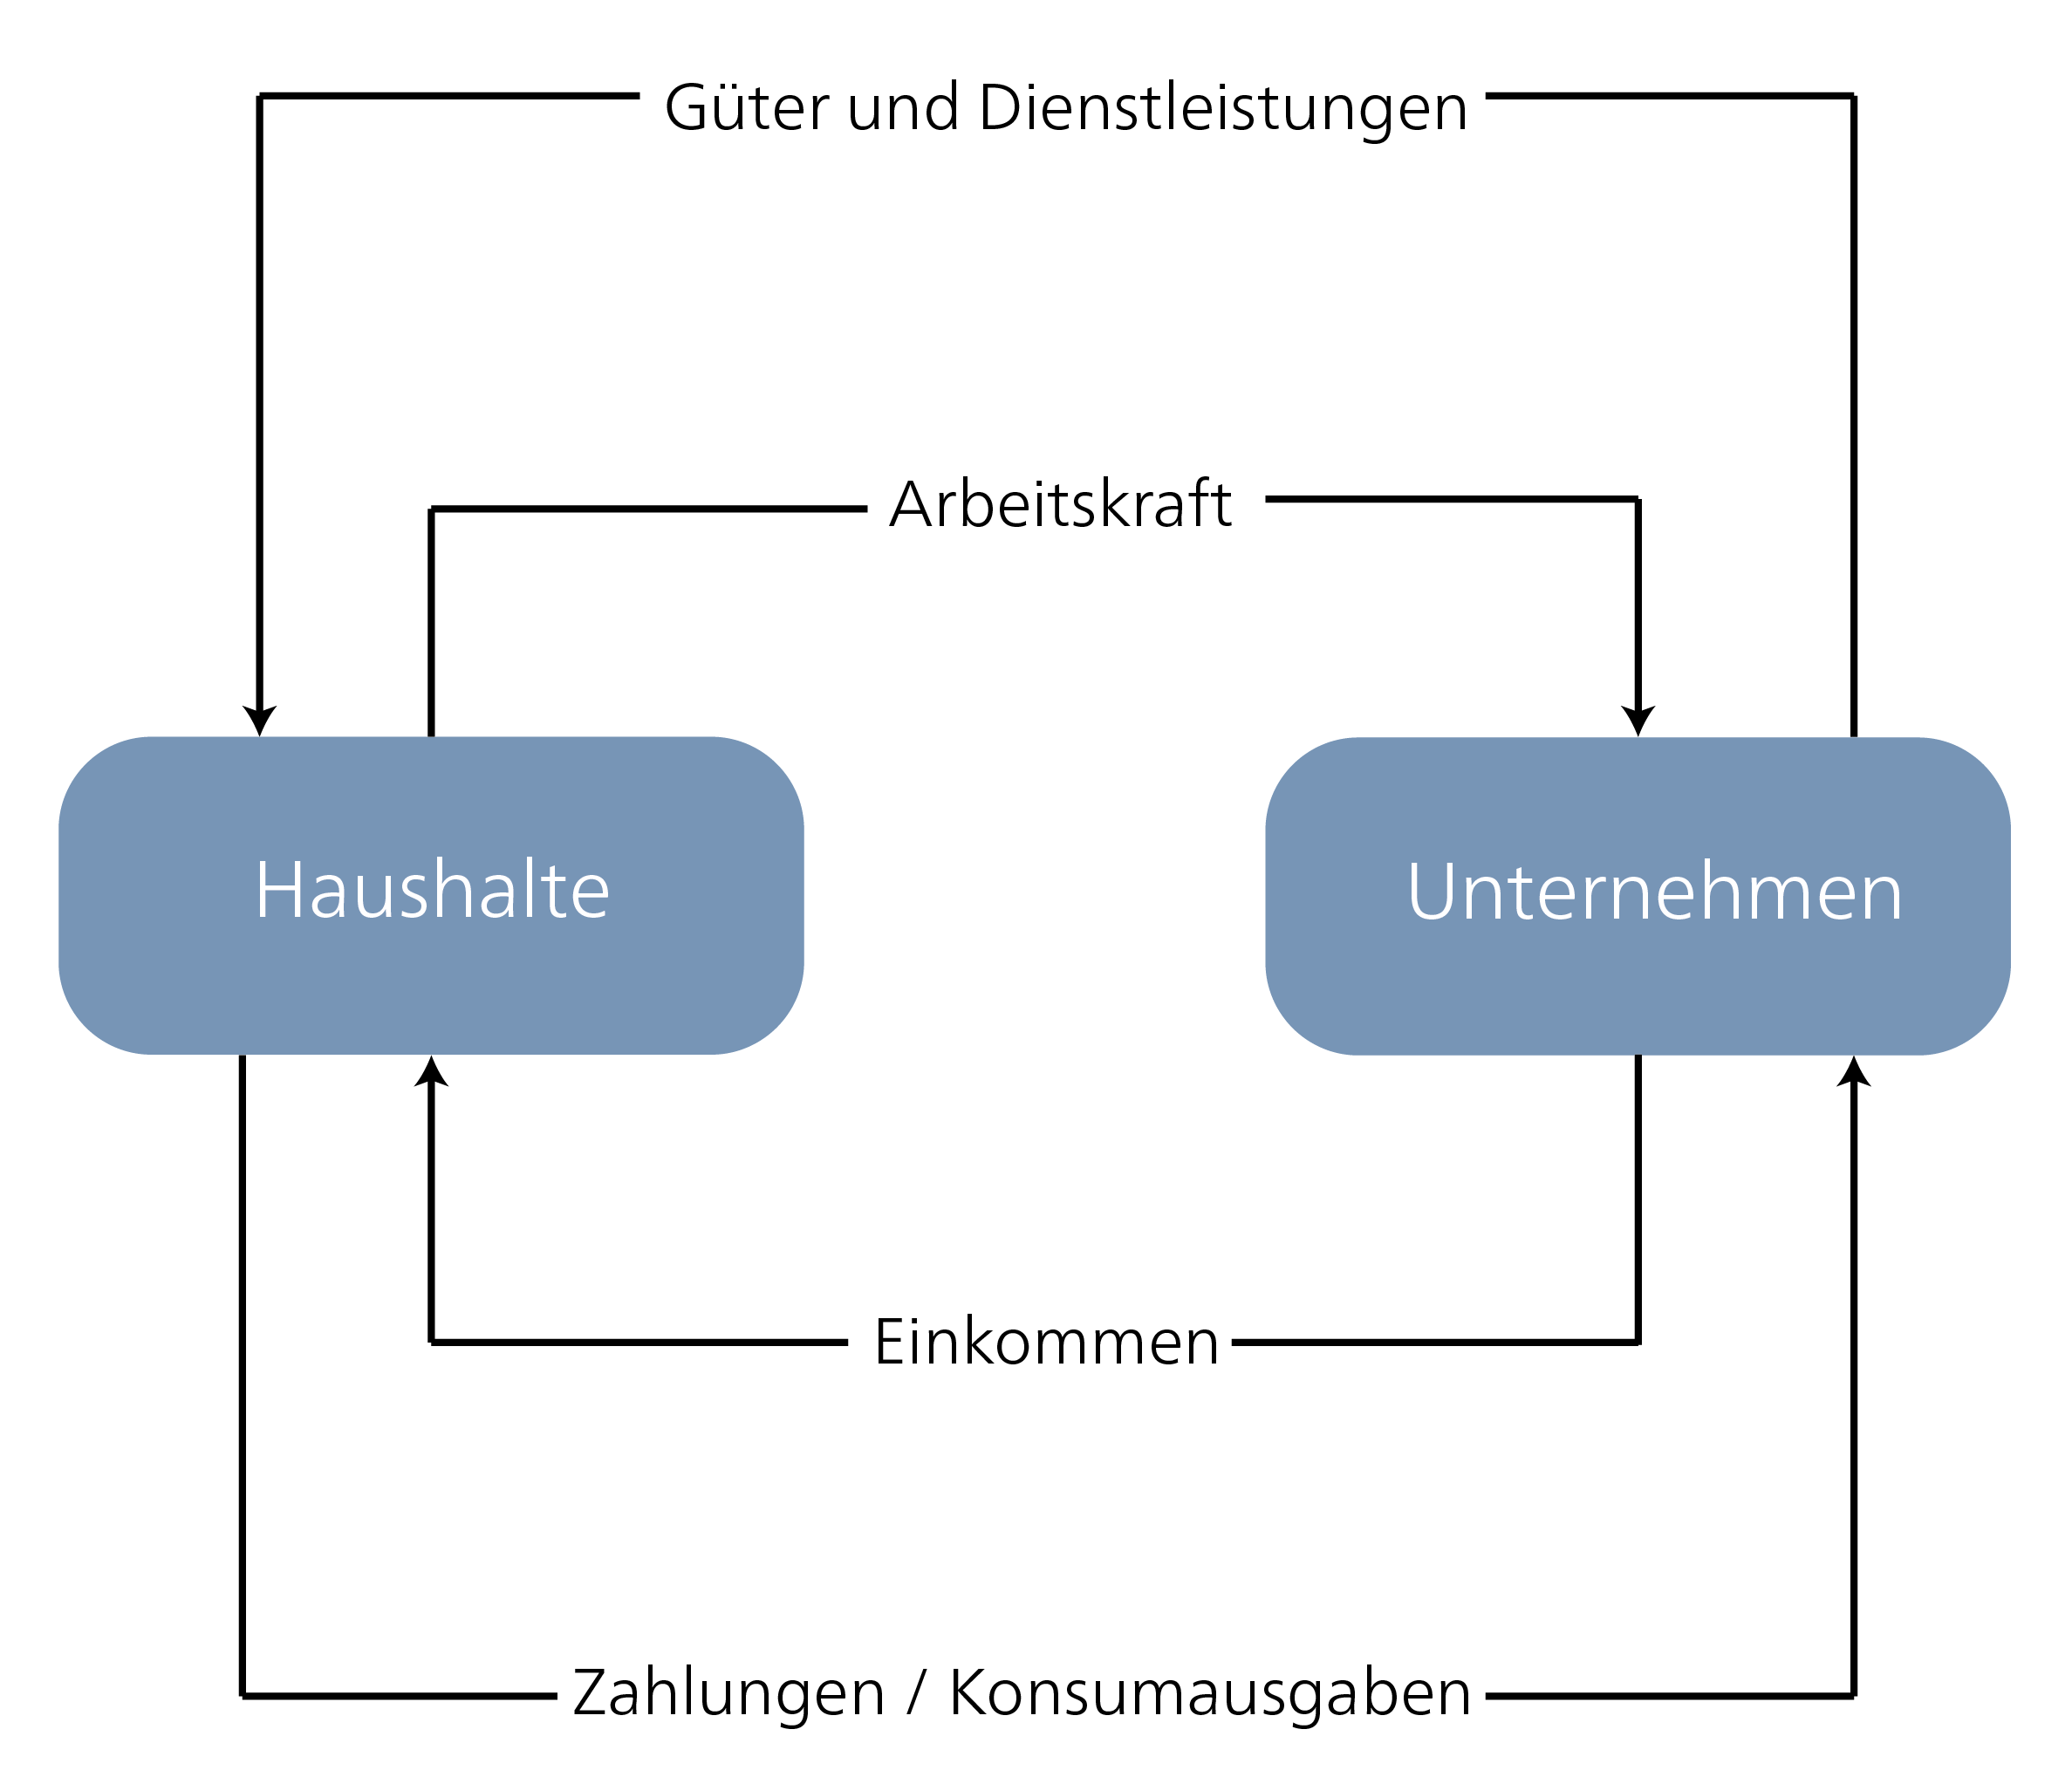
\includegraphics[keepaspectratio]{5_economic-sustainability/images/Fig5_2_EconCycle_simple.png}}

}

\caption{\label{fig-econ-cycle}\textbf{Einfacher Wirtschaftskreislauf}
-- Güter- und Geldflüsse zwischen Haushalten und Unternehmen: Arbeit im
Tausch gegen Einkommen, Konsumausgaben im Tausch gegen Güter.}

\end{figure}%

\end{minipage}%
%
\begin{minipage}[t]{0.50\linewidth}

\begin{figure}[H]

\centering{

\pandocbounded{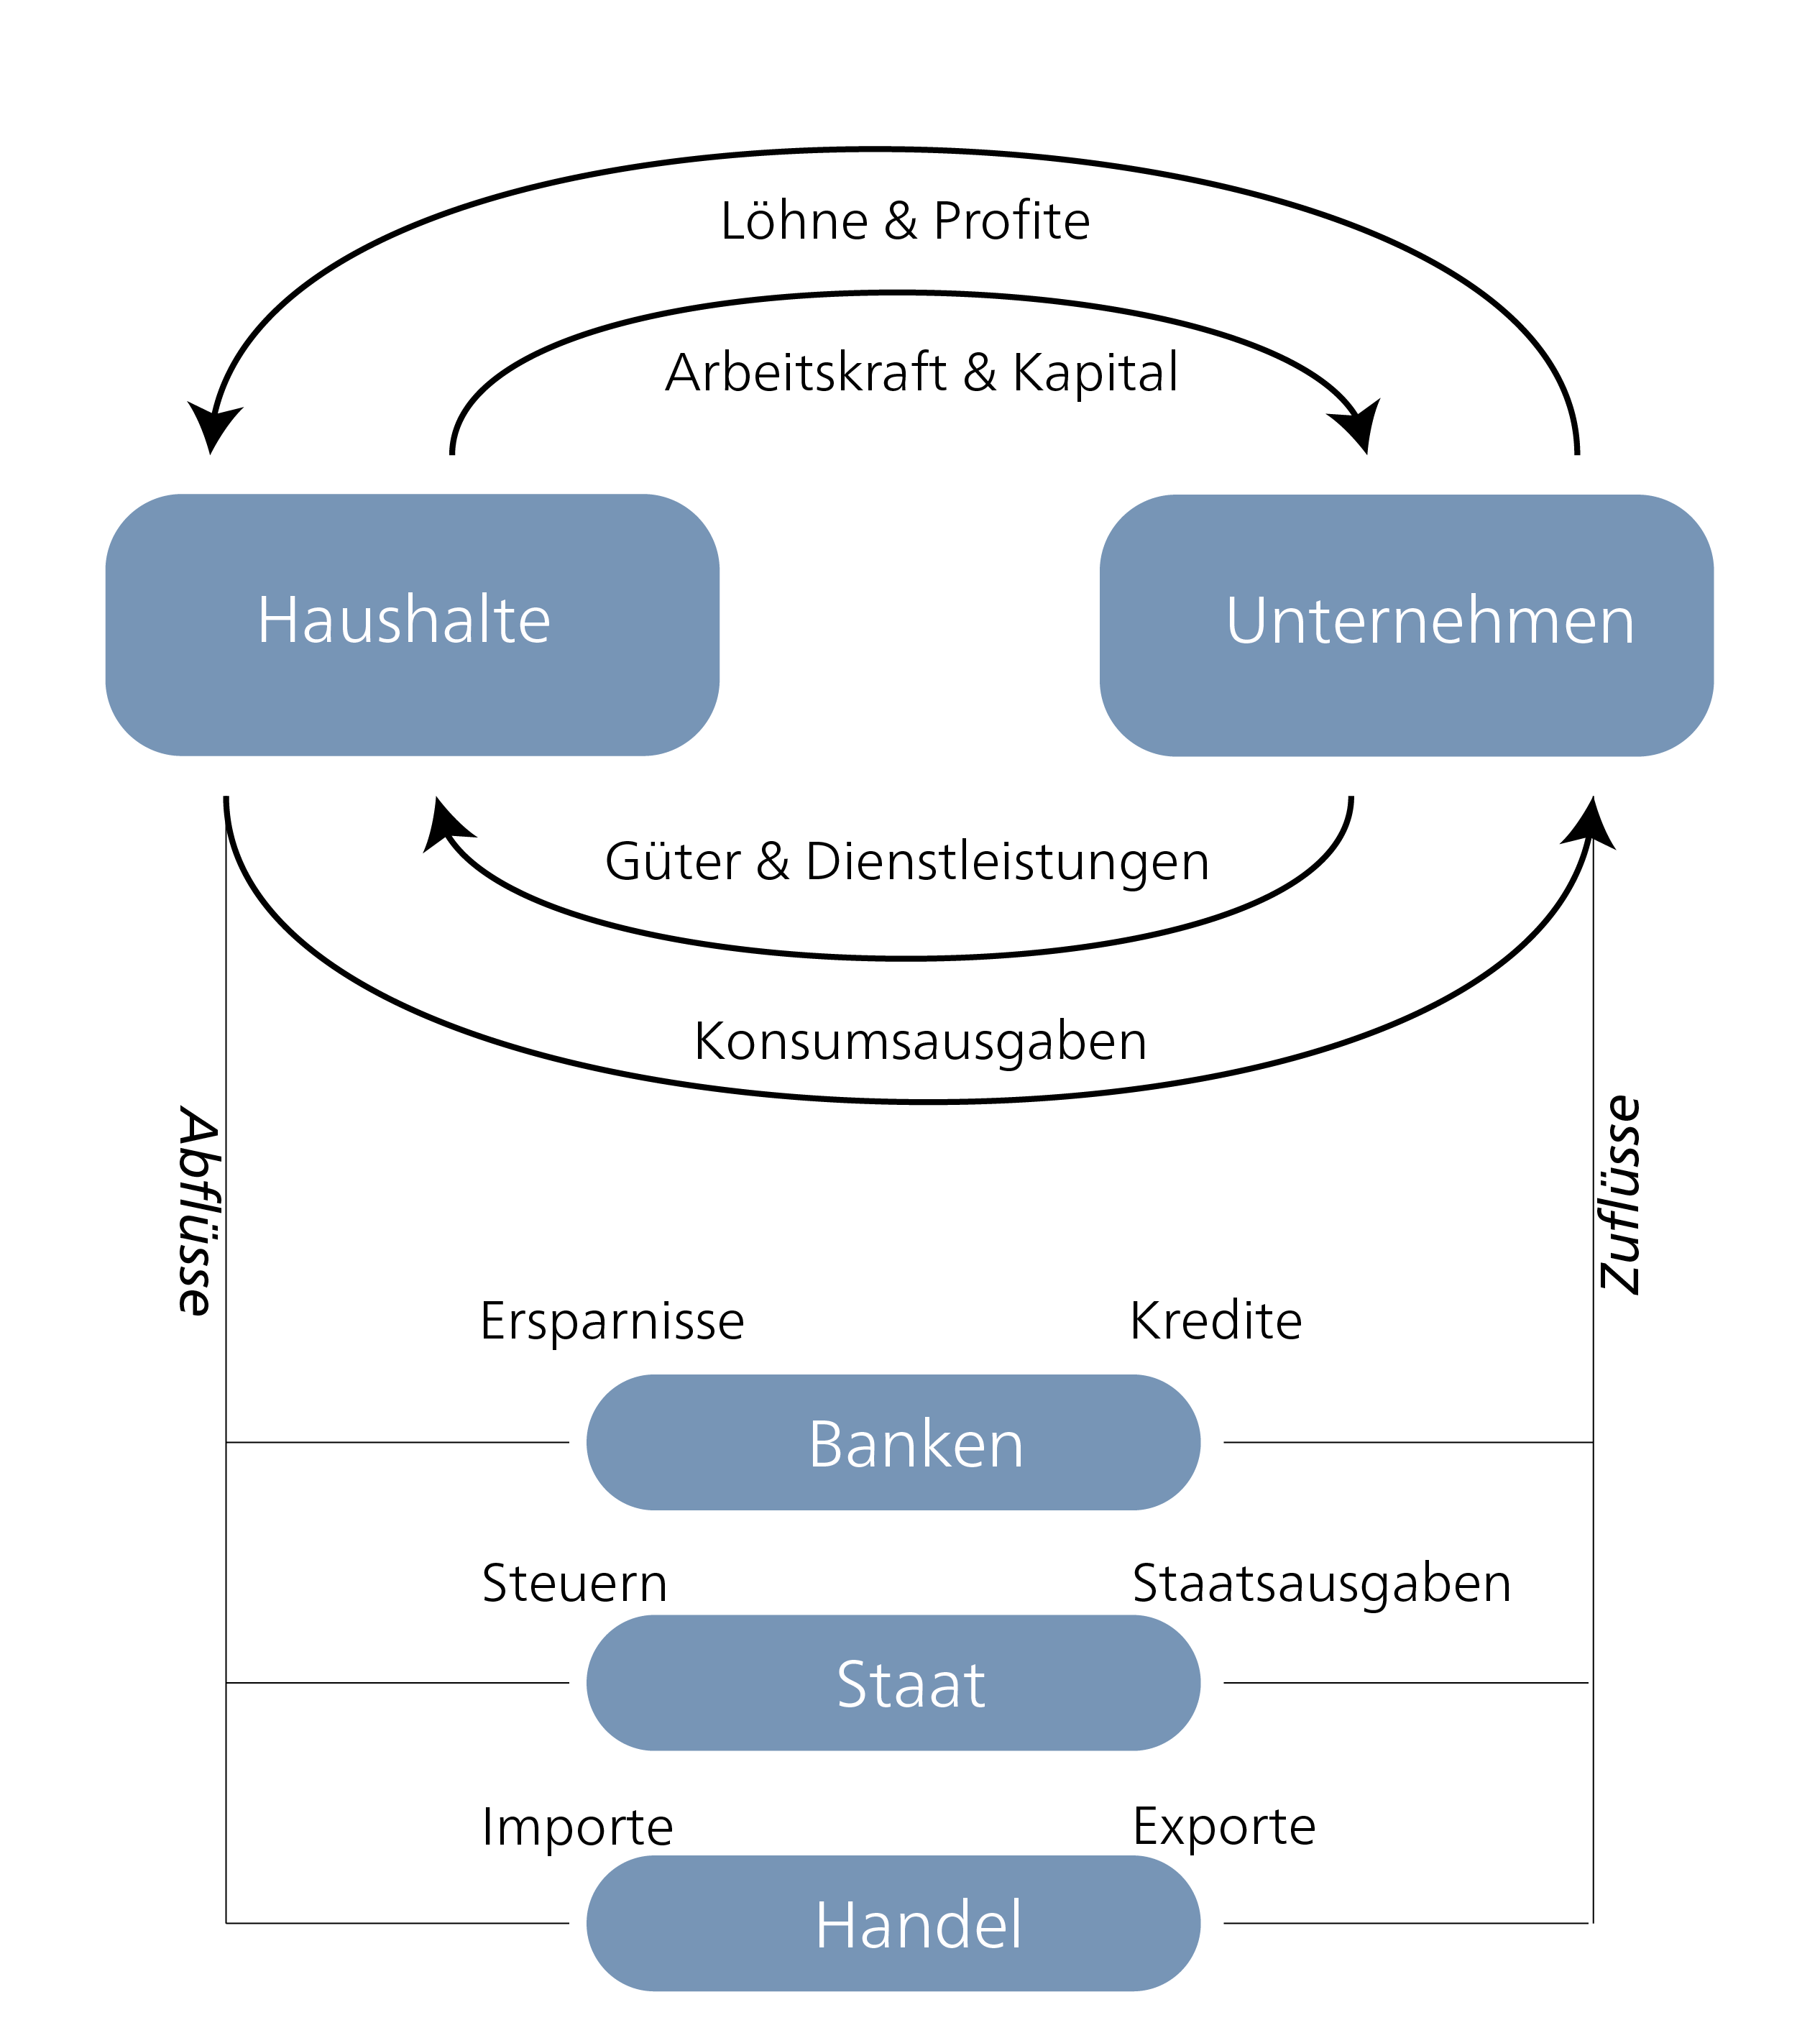
\includegraphics[keepaspectratio]{5_economic-sustainability/images/Fig5_2b_EconCycle_complex.png}}

}

\caption{\label{fig-ext-cycle}\textbf{Erweiterter Wirtschaftskreislauf}
-- Umfasst Banken, Staat und Aussenhandel und zeigt, wie Ersparnisse,
Steuern und Importe als \emph{Abflüsse} wirken, während Kredite,
Staatsausgaben und Exporte als \emph{Zuflüsse} fungieren.}

\end{figure}%

\end{minipage}%
\newline
\begin{minipage}[t]{0.50\linewidth}
Quelle: Eigene Darstellungen\end{minipage}%

\end{figure}%

\subsubsection{Kritik an der konventionellen
Wirtschaftskreislaufanalyse}\label{kritik-an-der-konventionellen-wirtschaftskreislaufanalyse}

Konventionelle Analysen des Wirtschaftskreislaufs stellen die
Marktwirtschaft typischerweise als wertschöpfende Einheit dar, wobei
Haushalte primär als Konsument*innen porträtiert werden. Grosse Teile
der Gesellschaft -- insbesondere unbezahlte Arbeit und
(Re-)Produktionsprozesse ausserhalb der Marktlogik -- werden weitgehend
ignoriert und damit implizit abgewertet. Feministische Wirtschaft
ergänzt daher ihre Darstellung der bezahlten Wirtschaft um unbezahlte
Bereiche (vgl. z. B. Elson 2000). Dennoch erinnert uns Mariana Mazzucato
(2018) daran, immer den sozialen Kontext zu berücksichtigen, in dem
solche Modelle entstehen:

\begin{quote}
„Es ist entscheidend, sich daran zu erinnern, dass alle Arten von
Buchführungsmethoden sich entwickelnde soziale Konventionen sind, die
nicht durch physikalische Gesetze und definitive ‚Realitäten' definiert
werden, sondern die Ideen, Theorien und Ideologien des Zeitalters
widerspiegeln, in dem sie entwickelt werden.'' (Mazzucato 2018, p.~76)
\end{quote}

Dies ermöglicht uns zu verstehen, warum Paul Samuelsons berühmtes
Kreislaufdiagramm der späten 1940er Jahre -- beeinflusst durch die
Erfahrungen der Grossen Depression und des Zweiten Weltkriegs -- sich
hauptsächlich auf den ununterbrochenen Einkommensfluss zur Förderung des
Wirtschaftswachstums konzentrierte. Nachfolgende Modelle des
Wirtschaftskreislaufs konzentrierten sich daher fast ausschliesslich auf
den Geldfluss zwischen Haushalten und Unternehmen.

Im Gegensatz dazu stellt Kate Raworth (2017b) die Wirtschaft als in
Gesellschaft und Umwelt eingebettet dar. Sie zeigt Haushalte, den Markt
(Unternehmen), Staaten und die Gemeinschaftsgüter (Commons) als
miteinander interagierend und berücksichtigt explizit ökologische
Grenzen. Dieses ganzheitlichere Verständnis ist entscheidend für ein
Umdenken wirtschaftlicher Aktivitäten im Sinne nachhaltiger Entwicklung.

\begin{tcolorbox}[enhanced jigsaw, arc=.35mm, bottomrule=.15mm, bottomtitle=1mm, breakable, colback=white, colbacktitle=quarto-callout-note-color!10!white, colframe=quarto-callout-note-color-frame, coltitle=black, left=2mm, leftrule=.75mm, opacityback=0, opacitybacktitle=0.6, rightrule=.15mm, title={Arbeit ist mehr als bezahlte Arbeit}, titlerule=0mm, toprule=.15mm, toptitle=1mm]

Arbeit ist ein zentraler Produktionsfaktor jeder Wirtschaft und
notwendig für die Umwandlung natürlicher Ressourcen in Güter und
Dienstleistungen. Wie diese Arbeit organisiert wird, hat sich im Laufe
der Geschichte verändert, abhängig von den verfügbaren Werkzeugen und
Technologien sowie den bestehenden Organisations- und Regierungsformen.
Arbeit ist daher kontextabhängig.

Neoklassische Wirtschaft konzentriert sich typischerweise auf bezahlte
Arbeit, die erst im Industriekapitalismus des 19. Jahrhunderts ihre
Schlüsselposition erlangte und sie im 20. Jahrhundert festigte.
Unbezahlte Arbeit (z. B. Haus-, Pflege-, Fürsorge- und Ehrenamtsarbeit),
die typischerweise von Frauen geleistet wird, wird weitgehend ignoriert
oder als selbstverständlich angesehen. Die Zahl der unbezahlten
Arbeitsstunden wird in der Schweiz seit 2000 erfasst, was zeigt, dass
der für unbezahlte Arbeit aufgewendete Zeitaufwand denjenigen für
bezahlte Arbeit übersteigt (BFS, Satellitenkonto Haushaltsproduktion
2020).

Aus der Perspektive wirtschaftlicher Nachhaltigkeit ist dieser enge
Ansatz problematisch. Schliesslich ist Arbeit nicht nur ein Inputfaktor,
sondern konstituiert wirtschaftliche Aktivität selbst -- sie ermöglicht
Produktion, Reproduktion und soziale Teilhabe. Eine nachhaltige
Wirtschaft erfordert daher ein weiteres Verständnis von Arbeit, das
sowohl bezahlter Arbeit als auch unbezahlter Reproduktionsarbeit
gleichermassen Rechnung trägt.

\end{tcolorbox}

\subsection{Staaten, Märkte und
Netzwerke}\label{staaten-muxe4rkte-und-netzwerke}

Wirtschaftssysteme unterscheiden sich darin, wie sie grundlegende Fragen
beantworten wie diese: „Wer produziert was, warum und für wen?``. Die
zwei Schlüsseldimensionen sind dabei Eigentum (privat oder öffentlich?)
und Koordination (zentral oder dezentral?). Aus „idealtypischer''
Perspektive ergeben sich folgende Grundformen (Basseler 2002):

\begin{itemize}
\item
  \textbf{Kapitalistische Marktwirtschaft}: Hier erfolgt die
  Koordination dezentral über Märkte, angetrieben durch das Wechselspiel
  von Angebot und Nachfrage („Bottom-up''). Die Produktionsmittel
  befinden sich überwiegend in Privatbesitz.
\item
  \textbf{Sozialistische, zentralisierte Wirtschaft}: In diesem Modell
  werden Produktions- und Verteilungsentscheidungen zentral durch
  staatliche Planung gesteuert („Top-down''). Die Produktionsmittel
  befinden sich generell in öffentlichem Besitz.
\item
  \textbf{Gemischte Wirtschaft (z. B. Wohlfahrtsstaat)}: Diese Systeme
  kombinieren Privateigentum an den Produktionsmitteln mit staatlicher
  Koordination in Schlüsselbereichen. Während die Ressourcenallokation
  weitgehend dezentral über Märkte erfolgt, greift der Staat ein, um sie
  zu regulieren und zu verteilen -- beispielsweise durch
  Sozialversicherungen, öffentliche Dienstleistungen oder progressive
  Steuerpolitik. Dieses Modell zielt darauf ab, Marktversagen zu
  korrigieren und soziale Gerechtigkeit zu fördern. Die Koordination
  erfolgt daher teilweise dezentral über Märkte und teilweise zentral
  über politische Institutionen.
\item
  \textbf{Gemeinschaftsbasierte Netzwerke und Commons-Wirtschaften}:
  Diese konzentrieren sich auf Selbstorganisation, dezentrale
  Kooperation und Gemeinschaftseigentum. Beispiele umfassen
  Solidarwirtschaft, Genossenschaften und gemeinschaftlich verwaltete
  Ressourcen (Commons).
\end{itemize}

Historisch war der industrielle Kapitalismus -- zumindest anfänglich --
das vorherrschende Modell nach der Industriellen Revolution. Im 20.
Jahrhundert nahm er verschiedene Formen an, vom starken nationalen
Wohlfahrtsstaat der Nachkriegszeit bis zu den marktorientierten
Globalisierungsmodellen, die seit den 1980er Jahren vorherrschen. Hall
und Soskice (2001) beschreiben diese als „Spielarten des Kapitalismus''.

Heute ist es leichter, sich das Ende der Welt vorzustellen als das Ende
des Kapitalismus, wie Slavoj Žižek (1994, 1) formuliert. Und dennoch
entstehen zunehmend Alternativen, die zeigen, dass eine solidarische
Wirtschaft nicht auf lokale Nischen beschränkt sein muss. Stattdessen
kann eine solche Wirtschaft global vorgestellt und gestaltet werden und
über markt- oder staatszentrierte Paradigmen hinausgehen. Netzwerke,
Commons und alternative Wirtschaftsformen gewinnen an Aufmerksamkeit, da
sie neue Wege eröffnen, wirtschaftliche Prozesse demokratischer,
resilienter und ökologisch nachhaltiger zu organisieren. In \emph{The
Zero Marginal Cost Society} entwirft Jeremy Rifkin (2014) beispielsweise
kollaborative Commons -- gemeinsam verwaltete Ressourcen, die durch
digitale Plattformen und dezentrale Kooperation ermöglicht werden.

\subsection{Kapitalismus als Ausgangspunkt für Fragen wirtschaftlicher
Nachhaltigkeit}\label{kapitalismus-als-ausgangspunkt-fuxfcr-fragen-wirtschaftlicher-nachhaltigkeit}

Viele Nachhaltigkeitsherausforderungen -- z. B. die Klimakrise, soziale
Ungleichheit, Ressourcenübernutzung, Finanzmarktturbulenz -- sind keine
isolierten Phänomene. Sie sind Ausdruck eines übergreifenden Kontexts,
d.~h. der strukturellen Dynamiken des modernen globalen Kapitalismus.
Dieses Lehrbuch nimmt daher eine systemische Perspektive ein, wie sie
von Wissenschaftler*innen wie Polanyi (1944), Brand und Wissen (2017),
Hickel (2020), Seidl und Zahrnt (2010), Schneidewind (2016) und
Binswanger (2006) vertreten wird. Aus dieser Perspektive erfordert eine
Hinwendung zur Nachhaltigkeit eine Auseinandersetzung mit unseren
zugrundeliegenden wirtschaftlichen Strukturen und ihren politischen und
kulturellen Voraussetzungen -- und damit mit dem kapitalistischen System
der Gegenwart.

In diesem Lehrbuch betrachten wir Kapitalismus nicht nur als
Wirtschaftssystem, sondern als das gegenwärtige Wirtschafts- und
Gesellschaftssystem in seiner Gesamtheit. Dies umfasst wirtschaftliche,
soziale, rechtliche, kulturelle und ökologische Strukturen und
Dynamiken, die alle miteinander interagieren (vgl. Kasten). Kapitalismus
ist kein natürlicher Zustand wirtschaftlicher Aktivität, sondern das
Ergebnis einer spezifischen historischen Entwicklung. Seine Wurzeln
reichen in das spätmittelalterliche Europa, insbesondere England,
zurück, wo durch die Aneignung von Land (eine Praxis, die als
„Einhegung'' bekannt ist), die Entstehung eines freien Arbeitsmarktes
und frühe Formen kapitalistischer Landwirtschaft entscheidende
institutionelle Grundlagen gelegt wurden (vgl. Wood 2017).

Die Industrielle Revolution im späten 18. und frühen 19. Jahrhundert
ermöglichte letztlich den historischen Durchbruch des Kapitalismus:
Technologische Innovationen, fossile Brennstoffe und umfangreiche
Kapitalinvestitionen schufen ein neues Produktionssystem, das auf
Massenproduktion und Massenkonsum basierte. Dieser Prozess verfestigte
frühere Entwicklungen zu einem dominanten Wirtschafts- und
Gesellschaftssystem, das noch heute zentrale globale Strukturen prägt.

Dieses System ist als kapitalistische Produktionsweise bekannt, und
seine zugrundeliegende Logik ist durch drei Grundmerkmale
gekennzeichnet:

\begin{itemize}
\item
  die Trennung von Kapital und Arbeit, sodass Arbeiter*innen im
  Allgemeinen nicht die Produktionsmittel besitzen und daher gezwungen
  sind, ihre Arbeitskraft gegen Lohn zu verkaufen
\item
  Privateigentum an den Produktionsmitteln
\item
  die Ausrichtung auf Gewinnmaximierung und Gewinnverwendung
\end{itemize}

Kapitalist*innen -- als Eigentümer*innen der Produktionsmittel --
bringen Kapital, Land und Arbeit zusammen, um Güter und Dienstleistungen
in einem Produktionsprozess herzustellen. Das Ziel ist nicht primär die
Befriedigung von Bedürfnissen, sondern die Erzielung eines Tauschwerts,
der auf dem Markt erzielt werden kann -- mit dem Hauptzweck der
Kapitalvermehrung. Die Akkumulation von Kapital ist der wichtigste
Treiber und die strukturelle Logik der kapitalistischen
Produktionsweise. Ein wesentliches Merkmal dieses Prozesses ist die
Erzeugung von Mehrwert, d.~h. des wirtschaftlichen Werts, den
Arbeiter*innen in der Produktion schaffen und der ihre Löhne übersteigt.
Dieser Mehrwert bildet die Grundlage für Gewinne und wird auf
verschiedene Weisen verteilt:

\begin{itemize}
\item
  Ein Teil fliesst als Lohn an die Arbeiter*innen
\item
  Ein Teil geht an Eigentümer*innen von Land oder natürlichen Ressourcen
  als Boden- oder Grundrente
\item
  Ein Teil geht als Zinsen und Finanzrenten an den Finanzsektor,
  insbesondere wenn das Kapital durch Fremdkapital finanziert wird
\item
  Der verbleibende Mehrwert umfasst die Gewinne, die auch durch
  Monopolrenten (z. B. durch Marktmacht) oder Markenrenten (z. B. durch
  immaterielle Vermögenswerte wie Reputation) ergänzt werden können
\end{itemize}

Die Senkung der Stückkosten spielt eine Schlüsselrolle dabei, die
Produktion rentabel zu machen und die Wettbewerbsfähigkeit zu sichern.
Technologische Innovationen und Investitionen in Maschinen, Fabriken und
Infrastruktur steigern die Produktivität erheblich. Energie ersetzt
zunehmend menschliche Arbeit; standardisierte Produktionsprozesse wie
das Fliessband steigern die Effizienz und ermöglichen die
Massenproduktion günstiger Konsumgüter. Wie Henry Ford treffend gesagt
haben soll: „Jeder Kunde kann sein Auto in einer beliebigen Farbe
lackiert bekommen, solange sie schwarz ist.''

Um jedoch einen Gewinn zu erzielen, bedarf es mehr als bloss
technologischer Effizienz. Andere kritische Faktoren umfassen die
Kontrolle über Märkte und Wertschöpfungsketten, den Zugang zu günstigen
Ressourcen, die Fähigkeit, Arbeit zu disziplinieren und zu
kontrollieren, sowie die Gestaltung institutioneller und politischer
Rahmenbedingungen. Das bedeutet, dass Gewinne auf der Grundlage
ungleicher Machtverhältnisse zwischen Unternehmen und Arbeiter*innen,
zwischen globalen Zentren und Peripherien, entlang von Lieferketten und
innerhalb von Eigentumsstrukturen geschaffen werden.

Damit die riesigen produzierten Gütermengen auch verkauft werden können,
ist eine homogene Massennachfrage erforderlich. Diese wird durch
steigende Löhne, eine Konsumkultur und ein soziales Modell gefördert,
das den Besitz standardisierter Konsumgüter mit Wohlstand und sozialem
Aufstieg gleichsetzt.

\begin{tcolorbox}[enhanced jigsaw, arc=.35mm, bottomrule=.15mm, bottomtitle=1mm, breakable, colback=white, colbacktitle=quarto-callout-note-color!10!white, colframe=quarto-callout-note-color-frame, coltitle=black, left=2mm, leftrule=.75mm, opacityback=0, opacitybacktitle=0.6, rightrule=.15mm, title={Was ist Kapitalismus?}, titlerule=0mm, toprule=.15mm, toptitle=1mm]

Kapitalismus ist eine historisch entwickelte Gesellschaftsform, in der
die Produktion primär für den Markt erfolgt, Privateigentum an den
Produktionsmitteln vorherrscht und die Akkumulation von Kapital
wesentlich ist. Seine grundlegende Dynamik ist der Einsatz von Kapital:
Geld (G) wird in Waren (W) investiert, die dann mit Gewinn verkauft
werden, woraus mehr Geld (G') entsteht, wie von Karl Marx beschrieben.

Die kapitalistische Produktionsweise basiert auf der Trennung von Arbeit
und den Produktionsmitteln. Das bedeutet, dass Menschen ihre
Arbeitskraft verkaufen müssen, um Zugang zu Ressourcen zu erhalten.
Diese Logik schafft strukturelle Abhängigkeiten, die über das
Wirtschaftssystem hinaus in alle Bereiche der Gesellschaft reichen.

Historisch gesehen hat sich der Kapitalismus nicht „natürlich''
etabliert, sondern wurde durch Prozesse politischer Enteignung,
kolonialer Expansion und rechtlicher Transformationen durchgesetzt (z.
B. Abschaffung der Commons, Monetarisierung von Arbeit, Schulpflicht zur
Disziplinierung).

\end{tcolorbox}

\begin{figure}[H]

\centering{

\pandocbounded{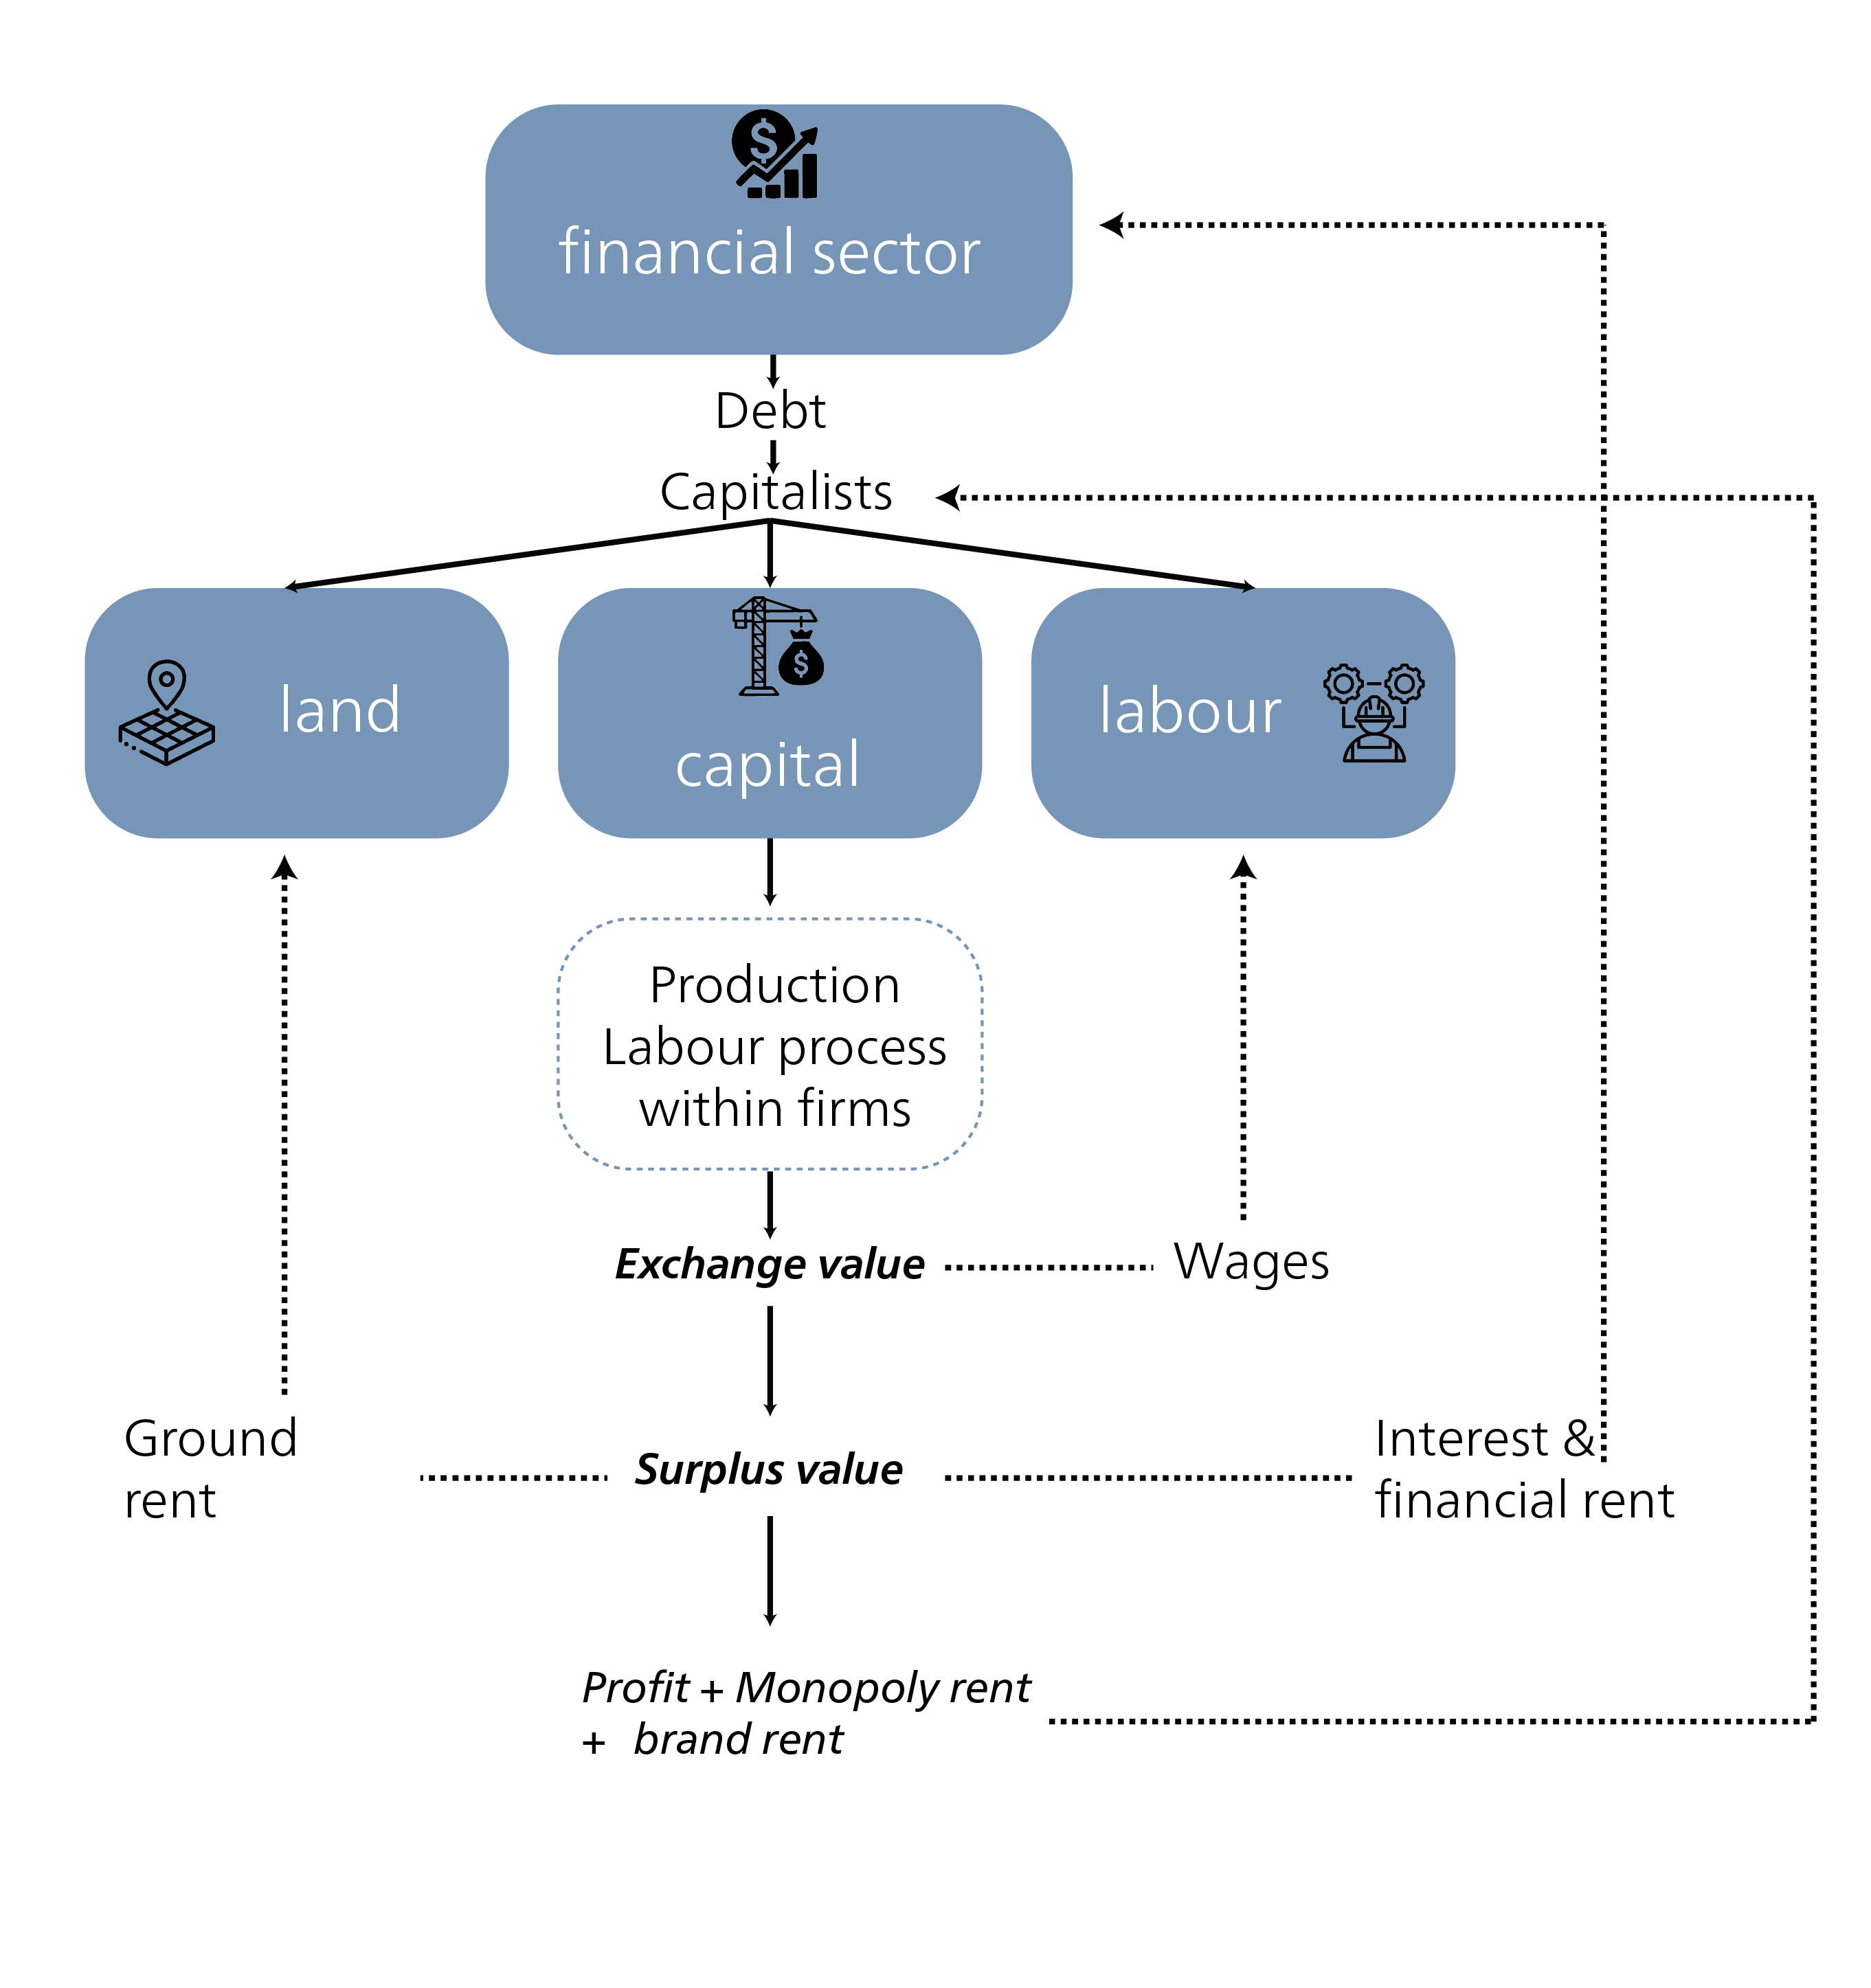
\includegraphics[keepaspectratio]{5_economic-sustainability/images/Fig5_4_ModeofProduction.png}}

}

\caption{\label{fig-mode-production}Kapitalistische Produktionsweise und
Verteilung des Mehrwerts. Der von Arbeiter*innen geschaffene Mehrwert
entsteht im Produktionsprozess und wird als Gewinn, Rente oder Zins
abgeschöpft. Kapitalist*innen verfolgen das Ziel der Kapitalvermehrung
durch die Kombination von Kapital, Land und Arbeit sowie mit der
Unterstützung von Krediten aus dem Finanzsektor. Quelle: Eigene
Darstellung, adaptiert nach Varoufakis (2024).}

\end{figure}%

Abbildung~\ref{fig-mode-production} veranschaulicht, wie das
kapitalistische Produktionssystem nicht nur Güter, sondern auch soziale
Verhältnisse produziert. Mit anderen Worten: Diejenigen, die Zugang zu
Kapital oder Land haben, können Mehrwert abschöpfen, während diejenigen,
die nur ihre Arbeitskraft besitzen, in der Regel nur Löhne erhalten. Der
Finanzsektor spielt dabei eine zunehmend bedeutende Rolle, indem er
Kapitalflüsse organisiert und durch Schulden zusätzlichen Zugang zum
Produktionsprozess gewinnt (vgl. Finanzialisierung und Finanzkrisen).
Diese Produktionsweise hat daher Auswirkungen weit über die
wirtschaftliche Sphäre hinaus. Der ungarische Wirtschaftssoziologe Karl
Polanyi beschrieb diesen Prozess als den Übergang zu einer
Marktgesellschaft: einer Gesellschaft, in der die Märkte nicht mehr in
sozialen und politischen Beziehungen eingebettet sind, sondern diese
zunehmend selbst bestimmen. Arbeit, Land und Geld wurden zu „fiktiven
Waren'' (Polanyi 1944) -- d.~h. zu Gütern, die ursprünglich nicht für
den Markt bestimmt waren, nun aber seiner Logik unterworfen sind. In
einer Marktgesellschaft sind Märkte nicht Teil der Gesellschaft -- die
Gesellschaft ist Teil des Marktes. Laut Polanyi führt dies zu
tiefgreifenden sozialen Erschütterungen -- z. B. in Form von sozialer
Unsicherheit, ökologischer Degradation oder wachsender Ungleichheit --
und erzeugt immer wieder Gegenbewegungen. Diese Dynamik ist eng mit zwei
zentralen Mechanismen kapitalistischer Expansion verknüpft:
Internalisierung und Externalisierung. Einerseits werden Ressourcen wie
Natur, Arbeit oder Wissen ohne marktmittelten Austausch angeeignet
(Internalisierung). Andererseits werden soziale Kosten auf Dritte
ausgelagert, wie künftige Generationen oder Länder des Globalen Südens
(Externalisierung). Eine ausführlichere Erläuterung dieser beiden
Begriffe findet sich im Kasten „Internalisieren und Externalisieren''.

In den folgenden Abschnitten analysieren wir, wie die kapitalistische
Produktionsweise, eingebettet in eine Marktgesellschaft, strukturelles
Wachstum erfordert und damit zu erheblichen Konflikten mit
Nachhaltigkeit führt.

\begin{tcolorbox}[enhanced jigsaw, arc=.35mm, bottomrule=.15mm, bottomtitle=1mm, breakable, colback=white, colbacktitle=quarto-callout-note-color!10!white, colframe=quarto-callout-note-color-frame, coltitle=black, left=2mm, leftrule=.75mm, opacityback=0, opacitybacktitle=0.6, rightrule=.15mm, title={Internalisieren und Externalisieren}, titlerule=0mm, toprule=.15mm, toptitle=1mm]

Der Preis eines Gutes spiegelt nicht immer seine tatsächlichen sozialen
Kosten wider. Wenn ein Gut zu einem Marktpreis produziert oder verkauft
wird, der diese Kosten ignoriert, werden sie häufig auf Dritte
übertragen -- wie Steuerzahlende, künftige Generationen oder die Umwelt.
Diese werden als externe Effekte oder Externalitäten bezeichnet, und sie
können positiv oder negativ sein. Externalitäten beeinflussen die
Produktions- und Konsumoptionen unbeteiligter Parteien.

Neoklassische Wirtschaft betrachtet externe Kosten generell als Anomalie
innerhalb eines ansonsten effizienten Marktes. Das übliche Gegenmittel
ist die „Internalisierung'' dieser Kosten -- z. B. durch Mechanismen wie
CO₂-Steuern. Im Gegensatz dazu argumentierte William Kapp bereits 1950,
dass je mehr ein System die private Gewinnmaximierung priorisiert, desto
grösser die Anreize sind, Kosten auf Menschen, Gesellschaft und Natur
abzuwälzen (Kapp 1950). Daher hat das derzeitige kapitalistische System
eine inhärente Tendenz, Kosten zu externalisieren. Stephan Lessenich
beschreibt die Wohlstandsgesellschaften im Globalen Norden als
Externalisierungsgesellschaften, die Kosten in den Globalen Süden
auslagern (Lessenich 2020). Gleichzeitig stützt sich die kapitalistische
Produktionsweise auf Internalisierungsprozesse: Natur, Arbeit oder
Wissen werden oft ohne Entschädigung angeeignet, basierend auf
strukturellen Machtverhältnissen. Beispiele umfassen Landraub,
unbezahlte Pflegearbeit und die Kommerzialisierung traditionellen
Wissens (vgl. z. B. Saave 2022).

Während liberale Markttheorien die Bedeutung von Preissignalen betonen,
stellen andere Denkschulen in Frage, ob wir wirklich allem einen Preis
zuweisen müssen, sogar der Natur. Diese grundlegenden Debatten sind
entscheidend für die Erreichung einer nachhaltigen Wirtschaft und werden
im Kurs \emph{Einführung in die nachhaltige Wirtschaft} vertieft
behandelt.

\end{tcolorbox}

\begin{tcolorbox}[enhanced jigsaw, arc=.35mm, bottomrule=.15mm, bottomtitle=1mm, breakable, colback=white, colbacktitle=quarto-callout-caution-color!10!white, colframe=quarto-callout-caution-color-frame, coltitle=black, left=2mm, leftrule=.75mm, opacityback=0, opacitybacktitle=0.6, rightrule=.15mm, title={Weiterführende Literatur}, titlerule=0mm, toprule=.15mm, toptitle=1mm]

\begin{itemize}
\item
  Polanyi, Karl. (1944) \emph{The Great Transformation: The Political
  and Economic Origins of Our Time}. Beacon Press.
\item
  Wood, Ellen Meiksins. 2017. \emph{The Origin of Capitalism: A Longer
  View}. Verso.
\item
  Göpel, Maja. 2016. `Why the Mainstream Economic Paradigm Cannot Inform
  Sustainability Transformations'. In \emph{The Great Mindshift: How a
  New Economic Paradigm and Sustainability Transformations Go Hand in
  Hand}, edited by Maja Göpel. Springer International Publishing.
  \url{https://doi.org/10.1007/978-3-319-43766-8_3}.
\end{itemize}

\end{tcolorbox}

\subsection{Wirtschaftswachstum: Entstehung, Normalisierung und
Kritik}\label{wirtschaftswachstum-entstehung-normalisierung-und-kritik}

Heute nehmen wir Wirtschaftswachstum als selbstverständlich hin, doch
aus historischer Sicht ist es ein jüngeres Phänomen. Jahrhundertelang
blieb das Niveau der wirtschaftlichen Produktion weitgehend stabil. Erst
mit der Industriellen Revolution in Grossbritannien am Ende des 18.
Jahrhunderts begann ein langsamer Anstieg, der ab den 1950er Jahren
deutlich an Fahrt aufnahm. Abbildung~\ref{fig-history-hockey-stick}
veranschaulicht eindrücklich, wie plötzlich und historisch einzigartig
diese Beschleunigung war. Über viele Jahrhunderte stagnierte das
Pro-Kopf-Einkommen, bevor es mit dem Aufstieg industrieller und
fossilbasierter Produktionsmethoden buchstäblich explodierte. Dieses
Wachstum konzentrierte sich jedoch hauptsächlich auf einige Länder des
Globalen Nordens. Drei Faktoren waren für diese Dynamik entscheidend:

\begin{enumerate}
\def\labelenumi{\arabic{enumi}.}
\tightlist
\item
  Der Wiederaufbau nach dem Zweiten Weltkrieg ermöglichte massive
  öffentliche und private Investitionen.
\item
  Der Zugang zu billigen fossilen Brennstoffen -- insbesondere Öl -- aus
  dem Nahen Osten senkte die Produktionskosten drastisch.
\item
  Das fordistische Konsummodell kombinierte hohe Löhne mit billiger
  Massenproduktion: Henry Fords Vision von „Autos für alle'' wurde zum
  Leitprinzip einer neuen Produktions- und Konsumlogik.
\end{enumerate}

\begin{figure}[H]

\centering{

\pandocbounded{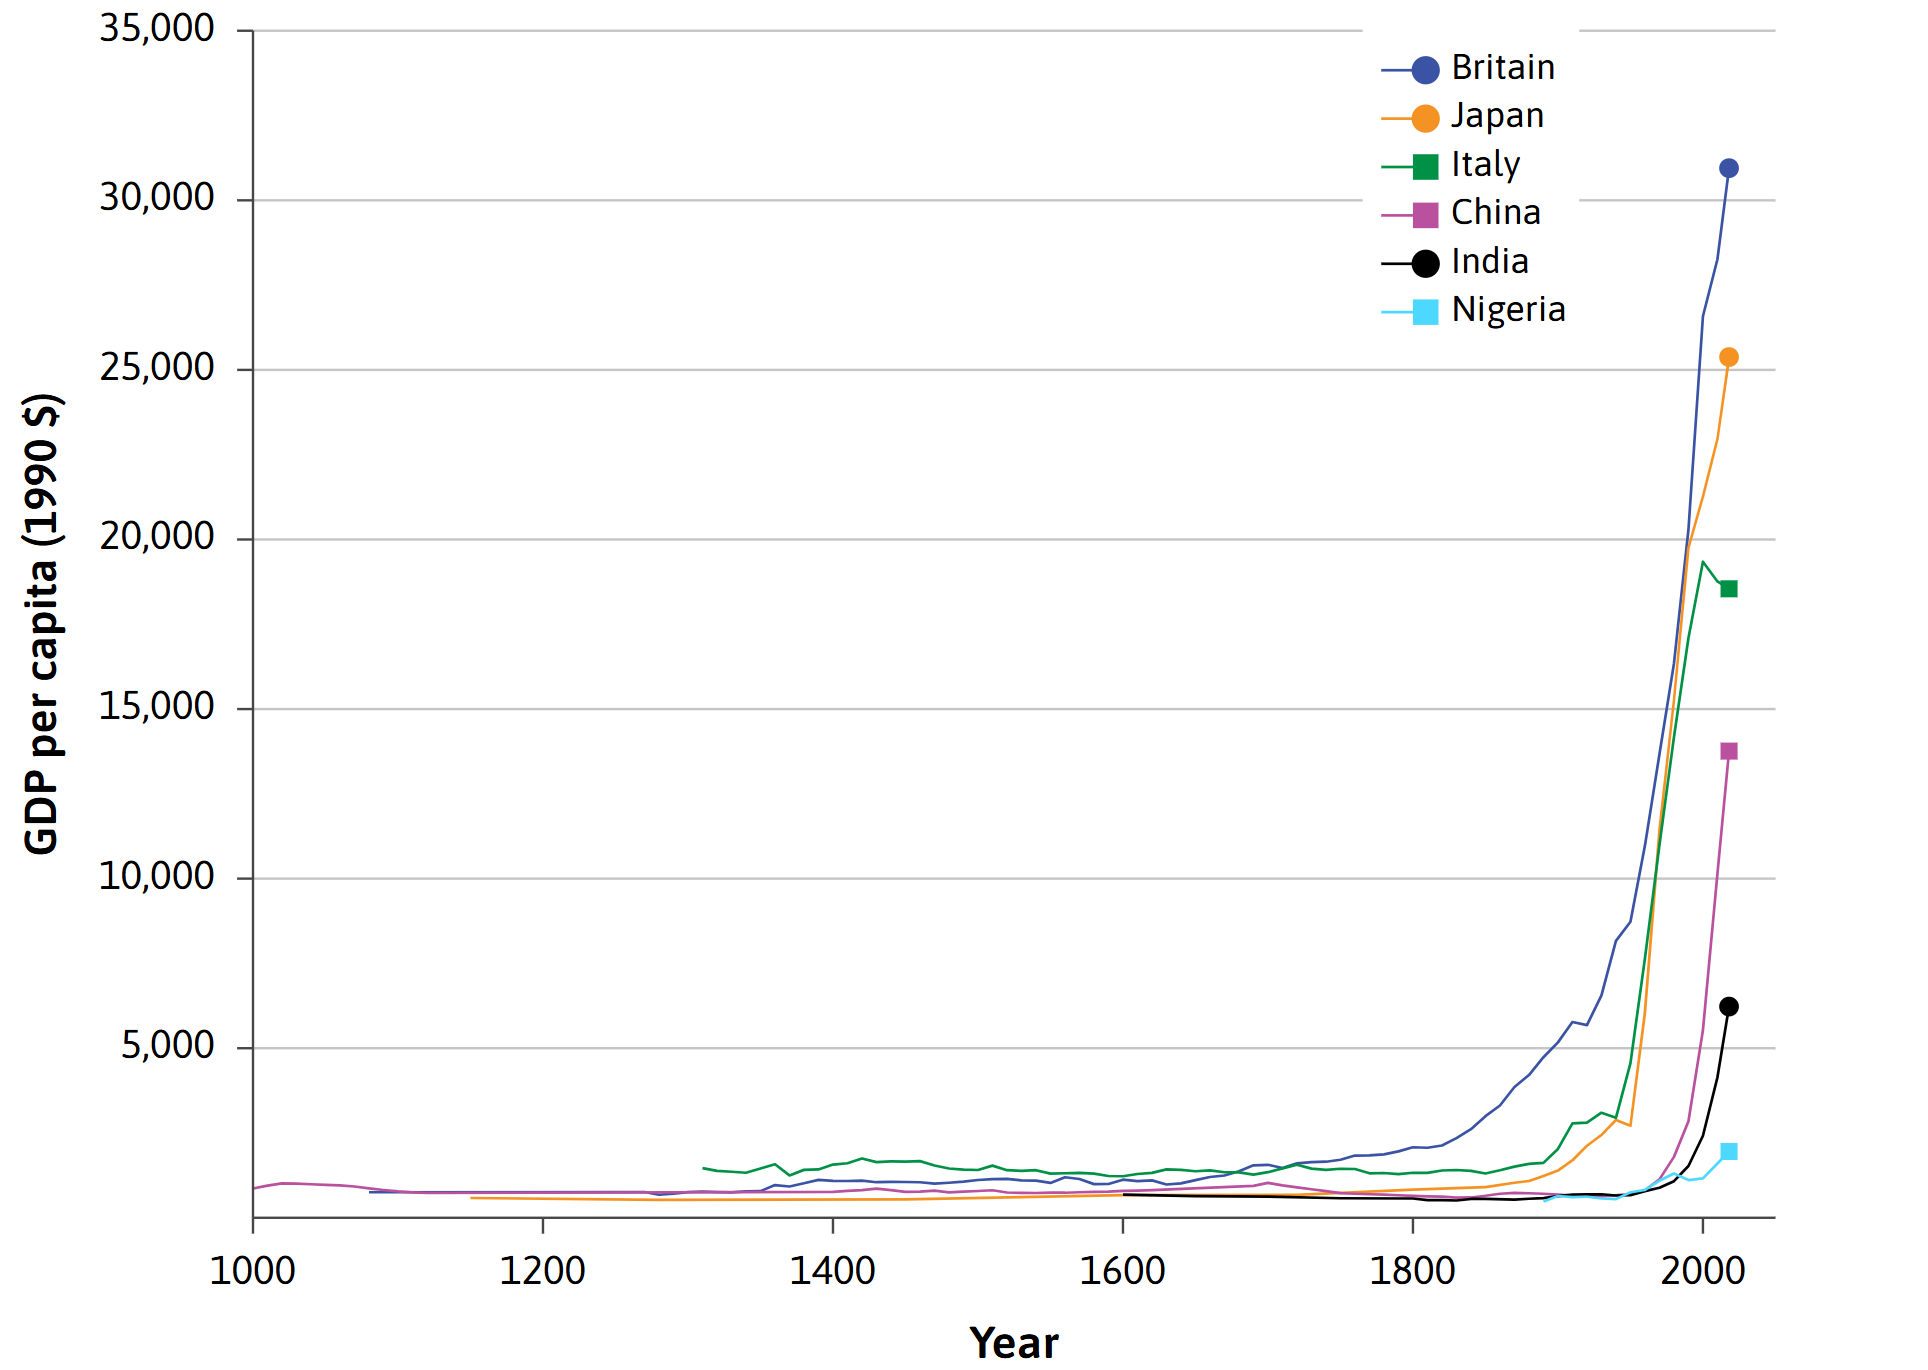
\includegraphics[keepaspectratio]{5_economic-sustainability/images/Fig5_5__GDP1000_2000.png}}

}

\caption{\label{fig-history-hockey-stick}Der Hockeyschläger der
Geschichte: Bruttoinlandsprodukt pro Kopf in fünf Ländern (1000--2018).
Das Pro-Kopf-Einkommen stagnierte jahrhundertelang. Erst mit der
Industriellen Revolution und dem fossilen Kapitalismus stiegen Einkommen
und Produktionsvolumen exponentiell -- wenn auch sehr ungleich von
Region zu Region. Quelle:
\url{https://books.core-econ.org/the-economy/microeconomics/01-prosperity-inequality-02-historys-hockey-stick.html\#figure-1-1}.}

\end{figure}%

Ein entscheidender Wendepunkt war, dass Kapital Land als zentralen
Produktionsfaktor ersetzte. Während Land naturgemäss begrenzt ist, hatte
Kapital -- verstanden als Maschinen, Technologie und Infrastruktur --
zunächst keine offensichtlichen Grenzen. Für Wirtschaftswissenschaftler
wie Malthus, der noch davon ausging, dass natürliche Ressourcen knapp
sind, war langfristiges Wachstum kaum vorstellbar. Die industrielle
Produktion unter kapitalistischen Bedingungen veränderte dieses
Paradigma grundlegend.

Wirtschaftswachstum führte dazu, dass das \textbf{Bruttoinlandsprodukt
(BIP)} als vorherrschendes Mass für Wohlstand in den Vordergrund rückte.
Das BIP misst den monetären Wert der in einem Land in einem bestimmten
Zeitraum (z. B. einem Jahr) produzierten Endgüter und Dienstleistungen,
misst aber keine unbezahlte Arbeit, ökologische Schäden oder soziale
Gerechtigkeit. Seit den 1980er Jahren gibt es auch eine Divergenz
zwischen steigendem BIP und stagnierender subjektiver
Lebenszufriedenheit. Das BIP eignet sich gut zur Beschreibung von
Marktaktivitäten -- aber nicht als umfassender Indikator für Wohlstand
oder Wohlbefinden.

Nach dem Zweiten Weltkrieg -- während der \emph{trente glorieuses} oder
„glorreichen Dreissig'' (1945--1975) -- wurde stetiges
Wirtschaftswachstum zur neuen Normalität. In dieser Zeit wurde häufig
diskutiert, ob zunehmender Wohlstand auf lange Sicht zu
Umweltverbesserungen führen könnte. Die Umwelt-Kuznets-Kurve (Stern
2004) legt nahe, dass die Umweltdegradation in den frühen Phasen des
Wirtschaftswachstums zunächst zunimmt, aber zurückgeht, sobald ein
bestimmtes Einkommensniveau erreicht ist, da Gesellschaften mehr in
Umweltschutz investieren. Die empirische Evidenz für diese Theorie ist
jedoch gemischt. Während einige lokale Umweltprobleme bewältigt wurden,
nehmen globale Umweltauswirkungen wie CO₂-Emissionen weiterhin zu. Ein
einfaches Fortsetzen des Wirtschaftswachstums garantiert daher
keineswegs einen reduzierten Druck auf die Umwelt und kann bestehende
planetare Grenzen weiter verschärfen (Wiedmann u.~a. 2020). Viele
soziale Teilsysteme, wie Sozialsicherungssysteme oder die
Arbeitsmarktpolitik, wurden darauf ausgelegt und strukturiert,
kontinuierlich steigende staatliche Einnahmen, Investitionen und
Beschäftigung zu erwarten. Diese strukturelle Wachstumsorientierung
wirkt sich bis heute aus und macht wirtschaftliche Nachhaltigkeit zu
einem systemischen Thema.

\subsection{Wachstumsabhängigkeit und strukturelle
Wachstumszwänge}\label{wachstumsabhuxe4ngigkeit-und-strukturelle-wachstumszwuxe4nge}

Da das derzeitige kapitalistische Wirtschaftssystem strukturell auf
Wachstum angewiesen ist, würde ein Rückgang der wirtschaftlichen
Aktivität (z. B. Stagnation, Rezession oder sogar Depression) zu einer
Wirtschaftskrise mit weitreichenden Konsequenzen für die Bevölkerung
führen (z. B. Arbeitslosigkeit, Armut, Kürzungen bei Sozialleistungen)
(Schmelzer und Vetter 2019, 26). Ohne Wachstum würde das System in einen
Krisenzustand geraten. Derzeit gibt es entweder Wachstum oder
Schrumpfung, aber nichts dazwischen. Matthias Binswanger (2019) zeigt,
dass der Wachstumsbedarf aus der Dynamik des Marktwettbewerbs
resultiert: Um wettbewerbsfähig zu bleiben, müssen Unternehmen
kontinuierlich expandieren und die Produktivität steigern -- sonst
riskieren sie den Verlust von Marktanteilen und Gewinnen oder sogar die
Insolvenz. Dieser Wachstumszwang zeigt sich auf makroökonomischer,
unternehmerischer und kultureller Ebene:

\textbf{Der makroökonomische Wachstumszwang} beschreibt die strukturelle
Abhängigkeit moderner Gesellschaften und Wirtschaftssysteme vom
Wirtschaftswachstum. Dieses Wachstum ist derzeit notwendig, weil viele
Kerninstitutionen und -systeme -- wie Arbeitsmärkte, Sozialsysteme und
öffentliche Finanzen -- nur dann stabil funktionieren können, wenn es
kontinuierliches Wachstum gibt. Es wird beispielsweise argumentiert,
dass ohne kontinuierliches Wachstum die Arbeitslosigkeit steigen würde,
da Unternehmen ihre Produktion und folglich ihre Belegschaft reduzieren.
Auch die öffentlichen Finanzen wären betroffen: Staatshaushalte, Renten
und Sozialsicherungssysteme basieren oft auf kontinuierlich steigenden
Einnahmen aus Steuern, die wiederum auf Wirtschaftswachstum angewiesen
sind. Nicht zuletzt verhindert Wachstum wirtschaftliche und politische
Krisen, da stagnierende oder schrumpfende Märkte von Unsicherheit,
Kapitalflucht und sozialer Unzufriedenheit begleitet werden können, was
politische Instabilität begünstigt (Seidl und Zahrnt 2010).

\textbf{Die unternehmerische Logik von Investition, Gewinn und
Expansion}. Unternehmen agieren innerhalb einer kapitalistischen
Produktionsweise, deren Logik auf kontinuierlichem Wachstum basiert.
Dieses Wachstum ist nicht nur wünschenswert -- es ist auch strukturell
erzwungen. Unternehmen investieren typischerweise nur dort, wo sie einen
Gewinn erwarten -- ein Prinzip, das in der Formel G--W--G'
(Geld--Ware--mehr Geld) zum Ausdruck kommt. Diese Dynamik wird durch den
Marktdruck intensiviert: Um wettbewerbsfähig zu bleiben, müssen
Unternehmen expandieren -- oder riskieren den Kollaps. Diese „Wachsen
oder Sterben''-Logik wird durch das Finanzsystem weiter verschärft. Von
investiertem Kapital werden kontinuierliche Renditen erwartet, es wird
verzinst. Um diesen Erwartungen gerecht zu werden, müssen Unternehmen
kontinuierlich Nachfrage generieren und in neue Produktionszyklen
investieren (vgl. Binswanger 2019). Unternehmen, die langfristig keine
Gewinne erzielen, verschwinden vom Markt. Wenn die Durchschnittsgewinne
in der gesamten Wirtschaft sinken, kann dies eine Kettenreaktion von
Unternehmensinsolvenzen auslösen -- mit potenziell schwerwiegenden
Auswirkungen auf Beschäftigung und soziale Stabilität.

Eine prägnante Einführung in die Logik des Kapitalismus gibt David
Graeber in diesem Kurzvideo:

\url{https://www.youtube.com/watch?v=QOVnb3y8hm4}

Massenkonsum und soziale Normen: Die Wachstumsspirale des
kapitalistischen Produktionssystems wird nicht nur durch technologische
und wirtschaftliche Faktoren angetrieben, sondern in erheblichem Masse
auch durch kulturelle Dynamiken. Heute dient Konsum nicht mehr nur der
Befriedigung unmittelbarer Bedürfnisse -- er erfüllt auch eine Vielzahl
sozialer Funktionen und ist zum Ausdruck von Status,
Selbstverwirklichung und Zugehörigkeit geworden. Wie im vorherigen
Abschnitt beschrieben -- und gemäss einer Schlüsselerkenntnis
keynesianischer Wirtschaftswissenschaftler*innen -- stimuliert
Massennachfrage Investitionen, die wiederum die Grundlage für
kapitalistische Gewinne auf makroökonomischer Ebene schaffen. Diese
Zusammenhänge verdeutlichen die Schlüsselrolle des Konsums im
kapitalistischen Produktionssystem: Mit anderen Worten, eine starke
Verbrauchernachfrage ist für ein dauerhaftes Wirtschaftswachstum
unerlässlich. Ein Nachfrageausfall -- z. B. wenn die Reallöhne
stagnieren oder sinken -- würde das kapitalistische System
destabilisieren. In den letzten Jahrzehnten wurden verschiedene
Strategien umgesetzt, um solche Nachfrageausfälle zu kompensieren:

\begin{itemize}
\item
  \textbf{Integration von Frauen in den Arbeitsmarkt}: In vielen
  Ländern, insbesondere in den USA, nahm der Zugang von Frauen zum
  Arbeitsmarkt in den 1970er und 80er Jahren erheblich zu. Dies diente
  nicht nur der Förderung der Gleichstellung -- es half auch, die
  Kaufkraft der Haushalte aufrechtzuerhalten -- wie populäre kulturelle
  Darstellungen der Situation zeigen, etwa Dolly Partons Hit „9 to 5''.
\item
  \textbf{Zunahme des Konsums auf Kredit}: Da es natürliche Grenzen
  sowohl für Arbeitskräfte als auch für tägliche Arbeitsstunden gibt,
  nahm der Konsum auf Kredit zu. So wie private Haushalte Geld borgten,
  um mangelnde Kaufkraft zu kompensieren, tat dies auch der Staat:
  Öffentliche Ausgaben z. B. für Infrastruktur, Sozialleistungen oder
  Steuererleichterungen in den 1980er Jahren wurden oft durch
  Staatsschulden finanziert, um die gesamtwirtschaftliche Nachfrage zu
  stabilisieren. Die Deregulierung der Finanzmärkte befeuerte diese
  Entwicklungen weiter. Seit der Finanzkrise 2008 spielen Zentralbanken
  durch geldpolitische Massnahmen wie niedrige Zinssätze und
  Anleihenankäufe eine zunehmende Rolle bei der Stabilisierung der
  Nachfrage.
\item
  \textbf{Bekämpfung der Konsumersättigung}: In wohlhabenden
  Gesellschaften, in denen viele Grundbedürfnisse bereits erfüllt sind,
  steht die Werbeindustrie vor der Herausforderung, neue Konsumbereiche
  zu erschliessen. Es geht zunehmend darum, Bedürfnisse zu schaffen
  statt zu erfüllen. Wie der Wirtschaftswissenschaftler Mathias
  Binswanger (2019) zusammenfasst: „Wir haben uns von einer
  Bedürfniserfüllungsgesellschaft zu einer
  Bedürfnisschaffungsgesellschaft entwickelt'' und fügt hinzu:
  \emph{„Noch vor einigen Jahren wussten die Menschen nicht, dass sie
  täglich ihre Herzfrequenz, Aktivitäten, verbrannten Kalorien und
  Schlaf aufzeichnen müssen. Aber dank der Bemühungen der
  Gesundheitsuhren-Hersteller wurde dieses Bedürfnis in ihnen ‚geweckt'
  und Gesundheitsuhren und Fitness-Tracker werden nun in grossen Mengen
  verkauft.''}
\end{itemize}

\subsection{Finanzialisierung und
Finanzkrisen}\label{finanzialisierung-und-finanzkrisen}

Ursprünglich waren die Finanz- -- sowohl Geld- als auch Kapital- --
märkte eng mit der Realwirtschaft verknüpft und stellten Liquidität für
die Produktion von Gütern und Dienstleistungen bereit. Es wurde daher
angenommen, dass diese beiden -- Finanzmärkte und Realwirtschaft -- in
etwa im Gleichschritt wachsen würden. Dies ist jedoch seit mehreren
Jahrzehnten nicht mehr der Fall. Ab den 1980er Jahren sind Geld- und
Kapitalmärkte viel schneller gewachsen und haben den Bezug zur
Realwirtschaft verloren.

Ein Grund für diese Entwicklung war die Deregulierung der
internationalen Finanzmärkte. Diese Deregulierungsmassnahmen wurden in
den 1980er und 1990er Jahren eingeführt, um die stockende
wirtschaftliche Entwicklung in Ländern wie dem Vereinigten Königreich
(unter der konservativen Premierministerin Margaret Thatcher) und den
USA (unter Präsident Ronald Reagan, dem ursprünglichen Befürworter des
Slogans „Make America Great Again'') anzukurbeln. Die Massnahmen wurden
mit dem Argument legitimiert, dass frühere Krisen aus ineffizienter
staatlicher Regulierung und Intervention resultierten, die angeblich die
Rationalität einzelner Marktteilnehmer*innen daran gehindert habe, ein
Marktgleichgewicht zu erreichen. Die weitreichende Deregulierung der
Finanzmärkte sollte selbstregulierende Mechanismen zur wirtschaftlichen
Stabilisierung ermöglichen. Die Deregulierung umfasste die Aufhebung des
Glass-Steagall-Gesetzes von 1933, das eine strikte Trennung von Kredit-
und Wertpapiergeschäften vorgeschrieben hatte. Dies ermöglichte es
Banken, beide Geschäfte gleichzeitig zu betreiben, was spekulative
Aktivitäten stark begünstigte. Die spekulativen Handelsvolumina schossen
anschliessend nach der Jahrtausendwende mit dem Aufkommen des
computergestützten Hochfrequenzhandels in die Höhe.

\begin{tcolorbox}[enhanced jigsaw, arc=.35mm, bottomrule=.15mm, bottomtitle=1mm, breakable, colback=white, colbacktitle=quarto-callout-note-color!10!white, colframe=quarto-callout-note-color-frame, coltitle=black, left=2mm, leftrule=.75mm, opacityback=0, opacitybacktitle=0.6, rightrule=.15mm, title={Was wir über Geld und Schulden verstehen müssen}, titlerule=0mm, toprule=.15mm, toptitle=1mm]

Geld ist weit mehr als nur ein neutrales Tauschmittel. Es erfüllt vier
zentrale Funktionen in modernen Wirtschaftssystemen:

\textbf{Tauschmittel}: Geld vereinfacht wirtschaftliche Transaktionen,
indem es die Notwendigkeit eines gleichzeitigen Austauschs von Gütern
und Dienstleistungen beseitigt.

\textbf{Wertaufbewahrungsmittel}: Geld kann gespart und später verwendet
werden, was langfristige Planung und Investitionen ermöglicht.

\textbf{Recheneinheit (Wertmesser)}: Geld bestimmt den „Wert'' von
Arbeit. Diese Bewertung ist jedoch kein objektives Mass, sondern ein
Ausdruck sozialer Machtverhältnisse und Ideologien.

\textbf{Ermöglicher der Kapitalakkumulation}: Im Kapitalismus wird Geld
investiert, um mehr Geld zu generieren. Diese Dynamik kann, wenn sie
unkontrolliert bleibt, zu einer zunehmenden Vermögenskonzentration
führen.

Durch diese letzte Funktion ist Geld eng mit Schulden verknüpft: Im
heutigen Finanzsystem wird der Grossteil des Geldes nicht durch
staatliche Münzprägung oder Zentralbankaktivitäten geschaffen, sondern
durch die Kreditvergabe privater Geschäftsbanken. Das bedeutet, dass
jedes Mal, wenn ein Kredit vergeben wird, neues Geld entsteht --
zusammen mit einer entsprechenden Schuld. Daher hat jedes Guthaben auf
der Habenseite eine Schuld auf der Sollseite (vgl. Graeber 2012). Ohne
laufende Schulden gäbe es kein Geldwachstum -- und damit kein
Vermögenswachstum. Dies gilt sowohl für private Haushalte als auch für
Regierungen. In einem System wachsender Ungleichheit sind
Schuldner*innen oft strukturell benachteiligt -- sie sind abhängig von
Kreditgeber*innen und Sparmassnahmen sowie politischen Zwängen
ausgesetzt.

Das heutige Finanzsystem schafft daher nicht nur wirtschaftliche,
sondern auch politische Abhängigkeiten. Wer Geld hat, kann nicht nur
konsumieren, sondern verfügt auch über Macht -- und kann sie z. B. durch
politischen Einfluss, Medieneigentum oder strategische Investitionen
ausüben. Finanzialisierung, Spekulation und globale Kapitalflüsse
verschärfen diese Entwicklung weiter.

\begin{quote}
„Die Kehrseite privater Vermögensakkumulation ist öffentliche und
private Verschuldung. Schulden können nur abgebaut werden, wenn
gleichzeitig Vermögen abgebaut werden.'' (Holzinger 2024, 89)
\end{quote}

\end{tcolorbox}

Deregulierung und ihre Folgen ermöglichten es Banken, ihre Kreditvergabe
erheblich auszuweiten -- zunehmend auch an Haushalte mit niedrigen
Kreditratings (d.~h. begrenzter Rückzahlungsfähigkeit oder geringer
Kreditwürdigkeit). Um die damit verbundenen Risiken zu mindern, wurden
die Kredite gebündelt und als scheinbar sichere „Subprime''-Anleihen
weiterverkauft. Solche Mechanismen legten letztlich den Grundstein für
die Finanzkrise von 2008, als sich herausstellte, dass ein grosser Teil
dieser Finanzprodukte auf hochriskanten Kreditvergaben basierte.

Diese Verschiebung der wirtschaftlichen Dynamik und Macht hin zum
Finanzsektor wird als Finanzialisierung bezeichnet. Sie schuf einen
Machtkomplex aus Zentralbanken, Geschäftsbanken, anderen
Finanzinstitutionen, privaten Pensionsfonds und Eigentümer*innen
verschiedener Vermögenswerte. In diesem Prozess wachsen die Finanzmärkte
im Verhältnis zur Realwirtschaft unverhältnismässig stark, ein Trend,
der durch nationale Deregulierungsmassnahmen begünstigt wird.
Finanzialisierung intensiviert den Wachstumszwang und erhöht nicht nur
die Ungleichheit, sondern auch die ökologische Fragilität,
beispielsweise durch spekulative Investitionen in Ressourcen, Rohstoffe
oder Land. Beispiele wie der Derivatehandel mit Nahrungsmitteln oder
Ressourcen zeigen, wie finanzierte Märkte soziale Vulnerabilitäten und
ökologische Risiken verschärfen können.

\begin{tcolorbox}[enhanced jigsaw, arc=.35mm, bottomrule=.15mm, bottomtitle=1mm, breakable, colback=white, colbacktitle=quarto-callout-note-color!10!white, colframe=quarto-callout-note-color-frame, coltitle=black, left=2mm, leftrule=.75mm, opacityback=0, opacitybacktitle=0.6, rightrule=.15mm, title={Was sind Derivate und wie tragen sie zur Finanzialisierung bei?}, titlerule=0mm, toprule=.15mm, toptitle=1mm]

Derivate sind Finanzinstrumente, deren Wert aus den zukünftigen Kursen
oder Preisen anderer Güter, Vermögenswerte oder Referenzwerte wie
Zinssätze, Rohstoffpreise oder Aktienindizes abgeleitet wird.
Verbreitete Derivate umfassen Optionen, Futures und Swaps. Beim
Derivatehandel findet keine reale wirtschaftliche Produktion statt -- es
werden keine Güter oder Dienstleistungen geschaffen. Derivate sollten
ursprünglich gegen Preisschwankungen „absichern'', z. B. im
Rohstoffhandel. Die zunehmende Deregulierung und Technologisierung der
Finanzmärkte führte jedoch zur weit verbreiteten Nutzung von Derivaten
als spekulative Anlageinstrumente. Dies trug erheblich zur Entkopplung
der Finanzmärkte von der Realwirtschaft bei und förderte einen massiven
Markt für Finanzwetten, der die realen Wirtschaftswerte, auf denen die
Derivate basieren, oft bei weitem übersteigt. Diese Dynamik ist eine
Schlüsselkomponente der „Finanzialisierung'' und erhöht die
wirtschaftliche Instabilität sowie soziale und ökologische Risiken.

\end{tcolorbox}

\begin{tcolorbox}[enhanced jigsaw, arc=.35mm, bottomrule=.15mm, bottomtitle=1mm, breakable, colback=white, colbacktitle=quarto-callout-caution-color!10!white, colframe=quarto-callout-caution-color-frame, coltitle=black, left=2mm, leftrule=.75mm, opacityback=0, opacitybacktitle=0.6, rightrule=.15mm, title={Weiterführende Literatur}, titlerule=0mm, toprule=.15mm, toptitle=1mm]

\begin{itemize}
\tightlist
\item
  Blakeley, Grace. 2019. \emph{Stolen: How to Save the World from
  Financialisation}. Repeater.
\end{itemize}

\end{tcolorbox}

\subsection{Unternehmen als Schlüsselakteure wirtschaftlicher
Nachhaltigkeit}\label{unternehmen-als-schluxfcsselakteure-wirtschaftlicher-nachhaltigkeit}

Unternehmen spielen eine Schlüsselrolle in wirtschaftlichen Prozessen:
Sie produzieren Güter und Dienstleistungen, schaffen Arbeitsplätze und
treiben Innovation voran -- und sind gleichzeitig bedeutende Verursacher
von Umweltschäden. Im Kontext wirtschaftlicher Nachhaltigkeit sollten
wir Unternehmen daher nicht nur als Teil des Problems, sondern auch als
Teil einer möglichen Lösung betrachten (Hoffman 2018).

Unternehmen sind Organisationen, die Produktionsfaktoren (Arbeit,
Kapital, Land) kombinieren, um Güter und Dienstleistungen herzustellen,
typischerweise für den Verkauf auf dem Markt. Traditionell war ihr
oberstes Ziel, mehr Einnahmen als Ausgaben zu erzielen und damit einen
Gewinn zu erwirtschaften. Dieses klassische Verständnis wurde stark von
der „Shareholder-Doktrin'' beeinflusst, die Milton Friedman in seinem
vielzitierten Aufsatz von 1970 in der New York Times, „The Social
Responsibility of Business is to Increase its Profits'', prägnant
formulierte. Friedman argumentierte, dass die einzige soziale
Verantwortung eines Unternehmens darin besteht, den Gewinn für seine
Eigentümer*innen -- die Aktionär*innen -- innerhalb der geltenden
Gesetze und Marktregeln zu maximieren. Manager*innen schulden daher
primär den Aktionär*innen Loyalität, nicht sozialen oder ökologischen
Zielen. Diese Sichtweise bildete die Grundlage für viele
wirtschaftspolitische Modelle und Managementpraktiken in der zweiten
Hälfte des 20. Jahrhunderts. Sie trug massgeblich dazu bei, dass
Unternehmen stark auf kurzfristige Renditen, gesteigerte Effizienz und
Kostensenkung ausgerichtet wurden -- oft auf Kosten sozialer
Gerechtigkeit oder ökologischer Nachhaltigkeit. Kritiker*innen vertreten
die Ansicht, dass diese Logik entscheidende soziale und planetare
Grenzen systematisch ignoriert und die Verantwortung primär auf
Einzelpersonen oder Staaten verlagert.

Im Kontext der Nachhaltigkeit steht dieser enge Fokus unter verstärkter
Beobachtung. Alternativen wie der „Stakeholder-Ansatz'' gewinnen an
Bedeutung, der Unternehmen nicht nur als Gewinnmaximierer für
Eigentümer*innen, sondern als gesellschaftlich eingebettete Akteure
betrachtet, die gegenüber diversen Stakeholdern verantwortlich sind,
einschliesslich Mitarbeitenden, Kund*innen, Lieferant*innen, lokalen
Gemeinschaften und der Umwelt. Unternehmen variieren auch erheblich in
Grösse und Organisationsform und umfassen kleine und mittlere
Unternehmen (KMU), grosse Konzerne, Sozialunternehmen, Genossenschaften
und andere alternative Geschäftsmodelle. Diese Vielfalt beeinflusst
massgeblich, wie Nachhaltigkeit strategisch verankert und praktisch
umgesetzt wird.

Dyllick und Muff (2016) kategorisieren Unternehmen in drei
Entwicklungsstufen, basierend auf ihrer Position zur Nachhaltigkeit. Die
erste Stufe, „Business-as-usual'', beschreibt Unternehmen, die
Nachhaltigkeit weitgehend ignorieren und ihre wirtschaftlichen
Aktivitäten ausschliesslich auf finanzielle Ziele ausrichten. In der
zweiten Stufe, „Corporate Sustainability 1.0 und 2.0'', beginnen
Unternehmen, Nachhaltigkeit durch Effizienzverbesserungen, Compliance
(d.~h. Einhaltung gesetzlicher und regulatorischer Anforderungen) und
die Integration von Corporate Social Responsibility (CSR) in ihre
Geschäftsstrategien anzugehen. Dies geschieht jedoch typischerweise ohne
grundlegende Änderung der Kerngeschäftslogik. Erst in der dritten Stufe,
„Sustainability 3.0'', rückt die systemische Transformation des
Unternehmens in den Vordergrund. Hier verfolgen Unternehmen einen
umfassenderen Zweck: Sie verpflichten sich explizit zum
gesellschaftlichen Wohlergehen und zur Einhaltung planetarer Grenzen und
integrieren diese Ziele umfassend in ihr Kerngeschäftsmodell.

Die dritte Stufe erfordert einen grundlegenden Perspektivwechsel:
Während Unternehmen in den früheren Stufen primär von innen nach aussen
agiert haben, indem sie ihre bestehenden Strukturen leicht angepasst
haben, erfordert Sustainability 3.0 einen „Aussen-nach-innen''-Ansatz:
Unternehmen müssen ihre Identität und strategischen Kernprozesse an
drängenden sozialen und ökologischen Herausforderungen ausrichten.

Dennoch bleiben viele Nachhaltigkeitsbemühungen an der Oberfläche.
Typische Herausforderungen sind „Cherry-Picking'' -- das Feiern leicht
erreichbarer Nachhaltigkeitsziele, während systemische Veränderungen
ausbleiben; Rebound-Effekte, bei denen Effizienzsteigerungen zu einem
Anstieg des Konsums führen; sowie die „Carbon Tunnel Vision'', ein enger
Fokus auf die Reduktion von CO\textsubscript{2}-Emissionen als
vermeintlich einzige Lösung für Nachhaltigkeitsfragen.

\section{Nachhaltigkeitsstrategien und -politiken für eine nachhaltige
Wirtschaft}\label{nachhaltigkeitsstrategien-und--politiken-fuxfcr-eine-nachhaltige-wirtschaft}

Eine wirtschaftliche Transformation hin zu nachhaltiger Entwicklung
erfordert gezielte Strategien, die bestehende Wachstumslogiken,
Machtverhältnisse und Marktmechanismen hinterfragen und neu gestalten.
Nachhaltigkeitsstrategien in der wirtschaftlichen Dimension fokussieren
typischerweise auf drei grundlegende Prinzipien: Effizienz, Konsistenz
und Suffizienz. Effizienz zielt auf einen ressourcenschonenderen Einsatz
bestehender Technologien ab, während Konsistenz darauf ausgerichtet ist,
wirtschaftliche Prozesse stärker an natürlichen biogeochemischen
Kreisläufen auszurichten -- etwa durch Kreislaufwirtschaft oder
erneuerbare Energien. Suffizienz geht darüber hinaus und fordert eine
Begrenzung von Konsum und Produktion sowie ein neues
Wohlstandsverständnis, das auf „genug'' statt „mehr'' beruht. Während
Effizienz und Konsistenz grösstenteils innerhalb bestehender
Marktlogiken realisierbar sind, erfordert Suffizienz ein tiefergehendes
Umdenken hinsichtlich sozialer Werte und Gerechtigkeit.

In jüngerer Zeit wurden viele spezifische Reformvorschläge formuliert,
die verschiedene Hebelpunkte in der Wirtschaft adressieren, etwa
Produktion, Konsum, Arbeit oder Finanzierung. Holzinger (2024)
diskutiert die Notwendigkeit eines wirtschaftlichen Paradigmenwechsels,
skizziert durch verschiedene thematische „Transformationen'':

\begin{itemize}
\item
  \emph{Transformation der Arbeit}, z. B. durch Arbeitszeitverkürzung,
  Ausbau der Sorgewirtschaft und Anerkennung unbezahlter Arbeit
\item
  \emph{Transformation der Besteuerung}, ausgerichtet auf ökologische
  Lenkungswirkungen und eine sozial gerechte Umverteilung
\item
  \emph{Finanzielle Transformation}, mit Fokus auf Gemeinwohl,
  demokratische Kontrolle und öffentliche Investitionen
\item
  \emph{Unternehmenstransformation}, mit Fokus auf transformative
  Unternehmen, die soziale Ziele vor Gewinn stellen
\item
  \emph{Konsumtransformation}, mit Fokus auf die Reduktion des
  Ressourcenverbrauchs durch kulturellen Wandel und Infrastruktur für
  weniger (z. B. Sharing, Reparatur)
\item
  Und Reformen in spezifischen Sektoren: z. B. Mobilitätswende,
  Energiewende, Ernährungswende.
\end{itemize}

Diese Reformvorschläge verdeutlichen, dass Nachhaltigkeit eine
Kombination verschiedener sektoraler Hebel erfordert: Statt rein
technischer Lösungen braucht es neue institutionelle, soziale und
kulturelle Leitplanken. Im Diskurs über wirtschaftliche Nachhaltigkeit
lassen sich diese vielfältigen Vorschläge in drei übergeordnete
Makrostrategien mit unterschiedlichen Grundannahmen und Zielen
einordnen:

\begin{figure}[H]

\centering{

\pandocbounded{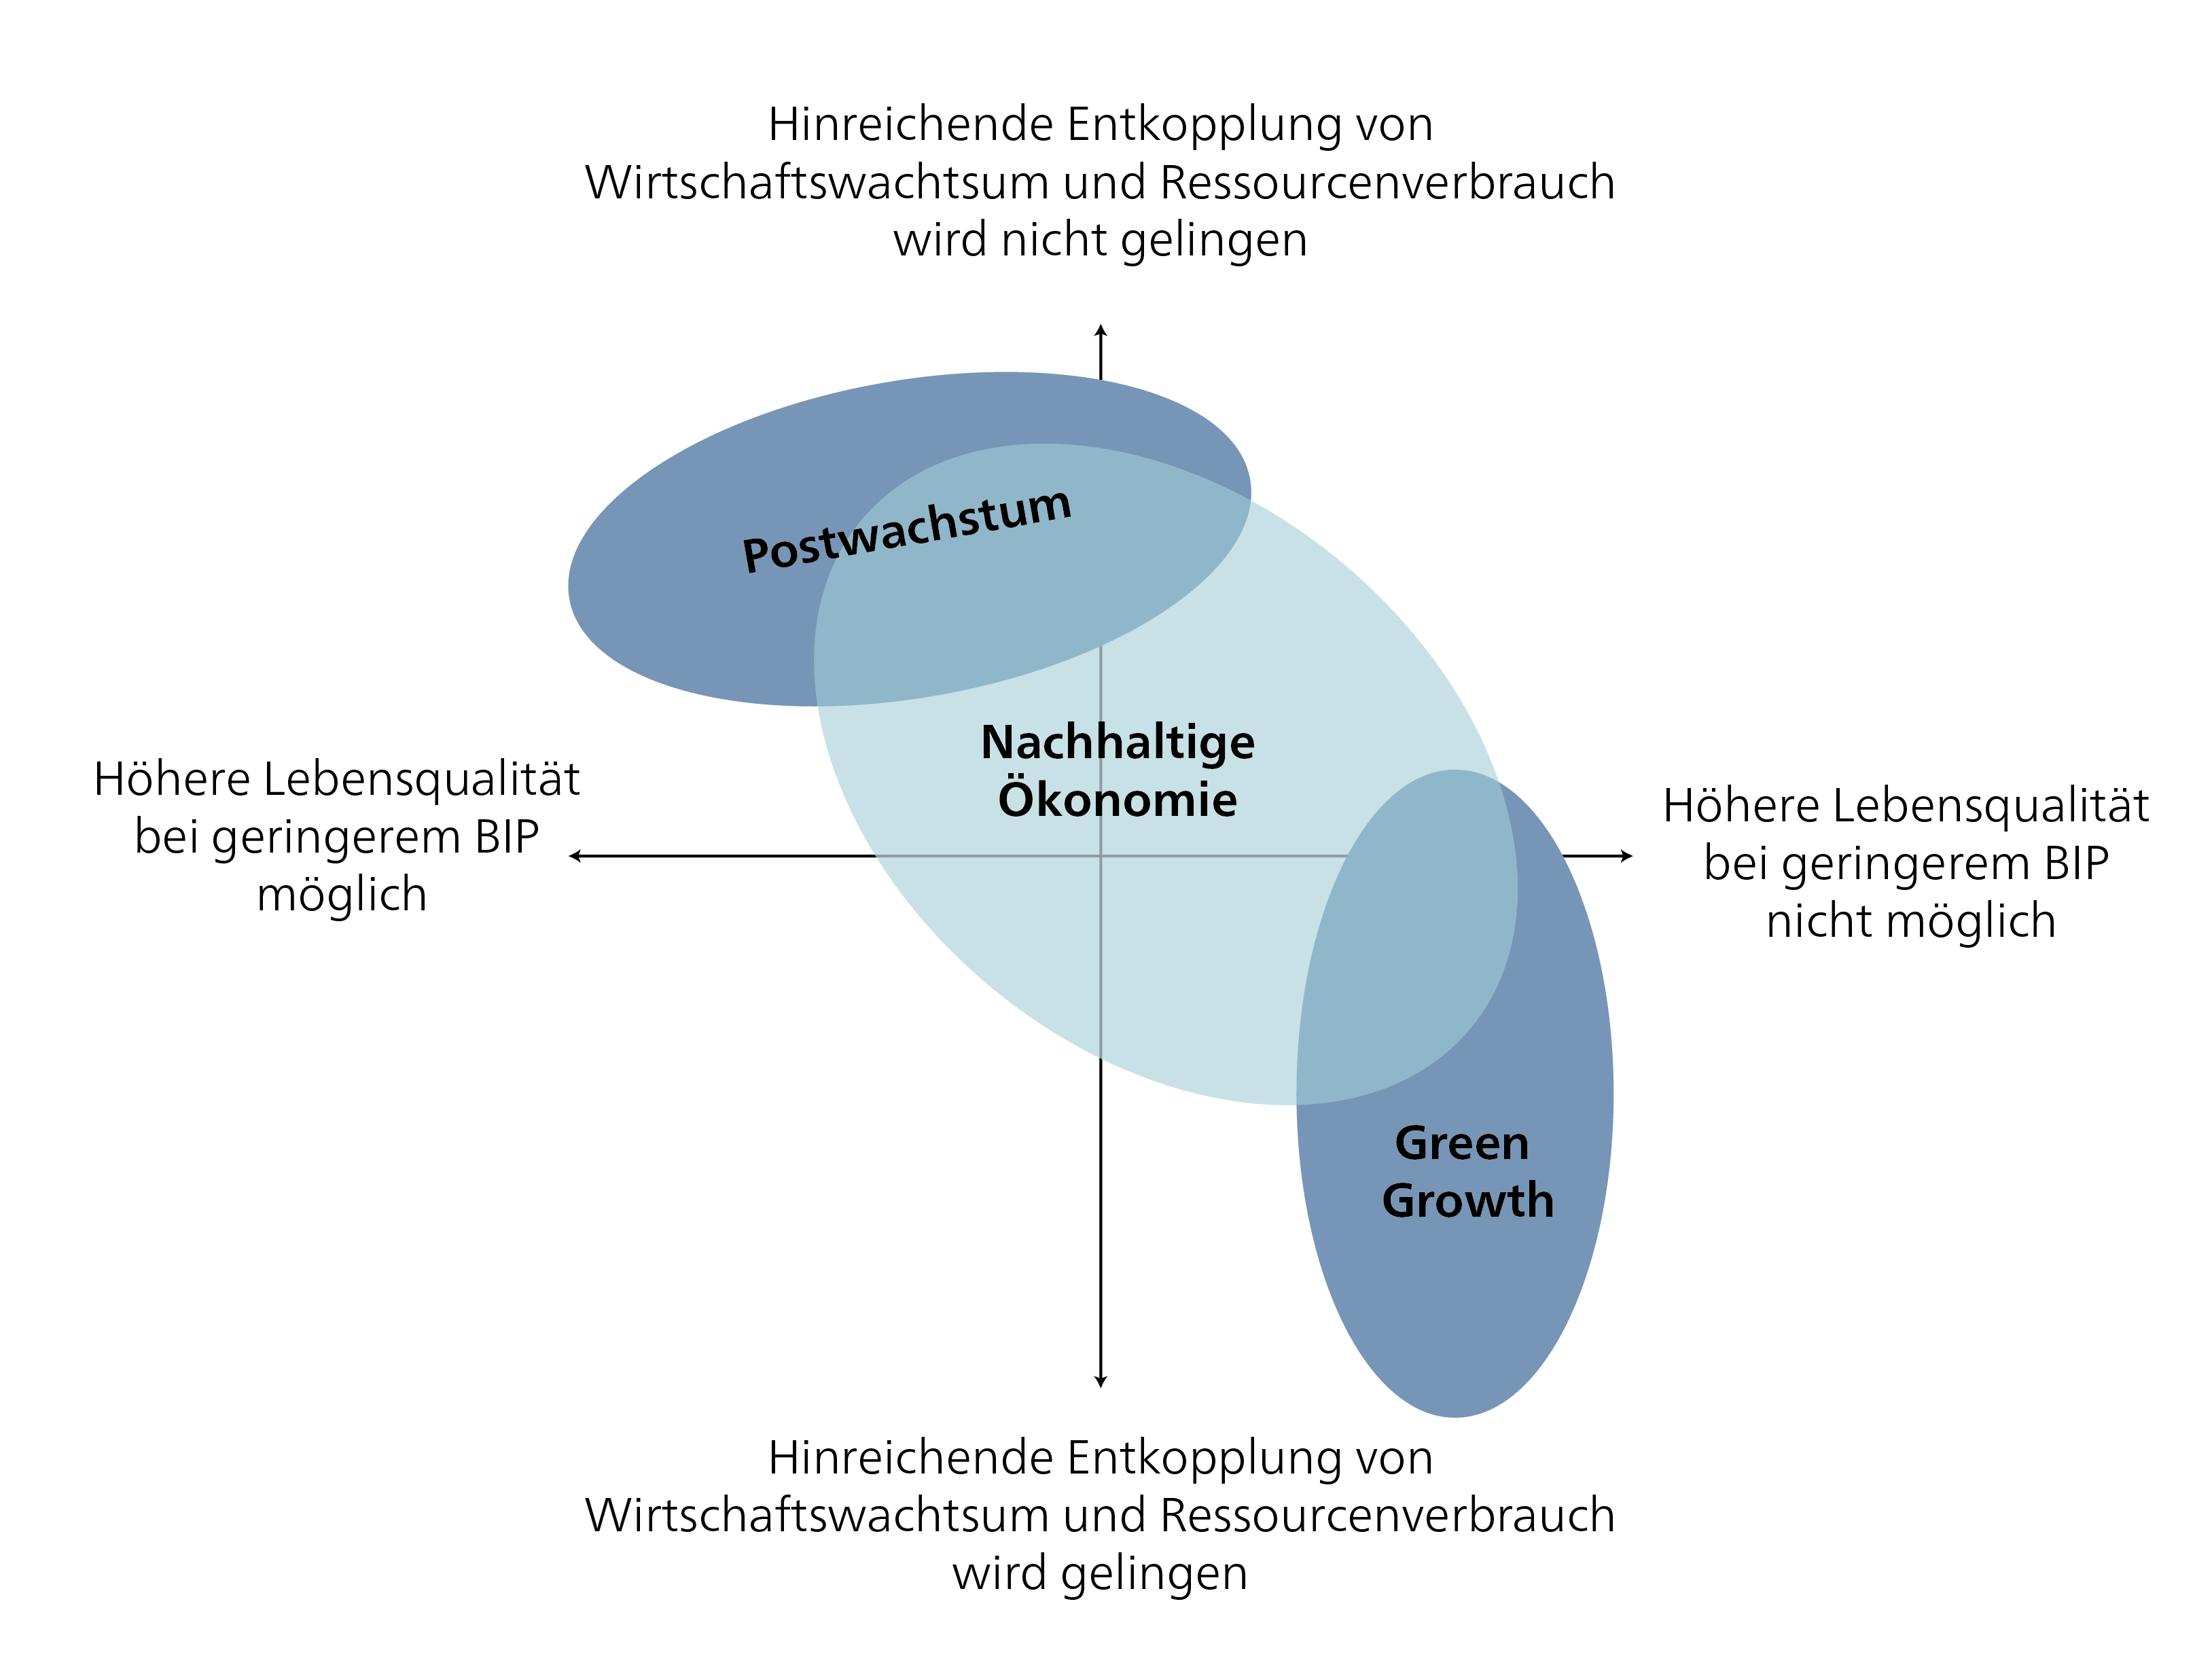
\includegraphics[keepaspectratio]{5_economic-sustainability/images/Fig5_6__NaÖk.png}}

}

\caption{\label{fig-naök}Positionierung von Green Growth, Degrowth und
Nachhaltige Wirtschaft anhand ihrer Annahmen über Entkopplung und das
Potenzial für hohe Lebensqualität bei niedrigerem BIP. Quelle: Eigene
Darstellung basierend auf Petschow (2018).}

\end{figure}%

\begin{itemize}
\item
  \textbf{Green Growth} fokussiert auf eine relative oder absolute
  Entkopplung von Wirtschaftswachstum und Umweltnutzung. Grüne
  Technologien, Effizienzsteigerungen und Umweltinnovationsmanagement
  dienen dazu, Umweltgrenzen einzuhalten -- ohne das Wachstumsparadigma
  grundsätzlich in Frage zu stellen.
\item
  \textbf{Degrowth (auch Postwachstum}\footnote{\textbf{Der Begriff
    Postwachstum wird ebenfalls häufig verwendet. Obwohl „Degrowth'' und
    „Postwachstum'' in vielen Forderungen und Analysen übereinstimmen,
    betont der Begriff Postwachstum stärker die Notwendigkeit
    wachstumsunabhängiger Institutionen, anstatt primär auf
    wirtschaftliche Schrumpfung zu fokussieren.}}** genannt)** hingegen
  zielt spezifisch darauf ab, wirtschaftliche Aktivitäten in Sektoren zu
  reduzieren, die besonders grosse Umweltschäden verursachen. Es geht
  nicht nur darum, ressourcenintensive Produktions- und Konsummuster
  rückgängig zu machen, sondern auch eine weitreichende soziale
  Transformation hin zu neuen Wohlstandsmodellen, Zeitwohlstand,
  Gerechtigkeit und Suffizienz zu erreichen. Im Mittelpunkt steht die
  demokratische Aushandlung kollektiver Bedürfnisse und die gerechte
  Verteilung von Arbeit, Einkommen und Ressourcen.
\item
  \textbf{Eine nachhaltige Wirtschaft} schlägt eine Brücke zwischen den
  beiden vorherrschenden Ansätzen Green Growth und Degrowth. Sie strebt
  nach sozialem Wohlergehen innerhalb planetarer Grenzen, ohne sich
  dogmatisch auf Wirtschaftswachstum oder -schrumpfung festzulegen.
  Petschow et al. (2020) beschreiben diese Position beispielsweise als
  \emph{vorsorgenden Postwachstumsansatz}.
\end{itemize}

\subsection{Nachhaltige Wirtschaft -- wachstumsunabhängige
Wirtschaftssektoren}\label{nachhaltige-wirtschaft-wachstumsunabhuxe4ngige-wirtschaftssektoren}

Viele Kerninstitutionen moderner Gesellschaften -- darunter Renten- und
Sozialsysteme, Arbeitsmärkte und öffentliche Finanzen -- sind derzeit
eng mit Wirtschaftswachstum verknüpft. Wie Seidl und Zahrnt (2010)
betonen, basieren diese Strukturen typischerweise auf impliziten
Wachstumsannahmen, die langfristig weder nachhaltig noch sozial gerecht
sind. Die Gestaltung wachstumsunabhängiger Institutionen ist daher
entscheidend. Dies würde nicht nur eine finanzielle Entkopplung von
Sozialsystemen und öffentlichen Finanzen vom BIP-Wachstum erfordern,
sondern auch die Überwindung der politischen Wachstumsfixierung, die
gegenwärtig viele wirtschaftspolitische Diskurse prägt. Reformen lassen
sich beispielsweise durch die Gestaltung neuer steuer- oder
finanzpolitischer Rahmenbedingungen umsetzen, die Stabilität auch ohne
Wachstum ermöglichen. Parallel dazu braucht es neue Produktions- und
Konsumformen:

\begin{itemize}
\item
  \emph{Ein suffizienter Lebensstil.} Eine kulturelle und
  infrastrukturelle Transformation hin zu suffizienten Lebensstilen
  bedeutet nicht nur den Verzicht auf Konsum auf individueller Ebene,
  sondern auch die Unterstützung neuer Produktions- und Konsummuster --
  z. B. durch Sharing-Modelle, eine Reparaturkultur, regionale
  Lieferketten oder die kollektive Nutzung von Ressourcen (vgl. u. a.
  Paech 2012)
\item
  \emph{Kollektives Handeln.} Die Entwicklung alternativer
  Infrastrukturen, solidarischer Kooperationsformen und
  nicht-kapitalistischer Produktionsweisen -- z. B. Commons,
  Genossenschaften oder kooperative Netzwerke -- wird von Autor*innen
  wie Muraca, Rifkin und Ostrom als tragfähige Zukunftsperspektive
  beschrieben. Solche Formen wirtschaftlicher Selbstorganisation stärken
  Resilienz, sozialen Zusammenhalt und ökologische Verantwortung.
\item
  \emph{Eine sorgende Wirtschaft.} Arbeit in Haushalten, in der Pflege
  und in der Gemeinschaft -- also reproduktive und sorgende Tätigkeiten
  -- muss systematisch aufgewertet werden. Statt Produktion und
  Reproduktion getrennt zu betrachten, betonen Ansätze wie jene von
  Biesecker und Hofmeister die Notwendigkeit, Sorgearbeit als Grundlage
  wirtschaftlicher Tätigkeit zu verstehen.
\item
  \emph{Überwindung der „imperialen Lebensweise''.} Aus globaler
  Perspektive wird die Nachhaltigkeitsdiskussion durch die Kritik an der
  „imperialen Lebensweise'' ergänzt. Autor*innen wie Brand oder Hickel
  zeigen, dass die wachstumsbasierte Lebensweise in einkommenstarken
  Gesellschaften auf der Externalisierung von Umwelt- und Sozialkosten
  in den Globalen Süden beruht. Eine nachhaltige Transformation muss
  daher auch internationale Machtverhältnisse und den Zugang zu
  Ressourcen kritisch hinterfragen.
\end{itemize}

Die Entwicklung wachstumsunabhängiger Wirtschaftssektoren erfordert
nicht nur neue Praktiken und kulturelle Modelle, sondern auch einen
gezielten politischen Rahmen, der diese Transformation unterstützt und
festigt. Ohne geeignete steuerliche, regulatorische und
investitionsbezogene Rahmenbedingungen bleiben suffiziente Lebensstile,
sorgende Wirtschaften oder commons-basierte Produktion oft auf Nischen
beschränkt. Die Aufgabe nachhaltiger Wirtschaftspolitiken besteht daher
darin, günstige Strukturen zu schaffen, destruktive Pfadabhängigkeiten
zu überwinden und neue Wirtschaftslogiken systematisch zu ermöglichen.
Die folgenden zentralen Politikinstrumente und makroökonomischen Hebel
könnten diese Transformation auf nationaler und internationaler Ebene
begleiten:

\begin{itemize}
\item
  \textbf{Verlagerung der Besteuerung von Arbeit hin zu Ressourcen und
  Kapital.} Während die Steuerlast in vielen Ländern derzeit stark auf
  die Besteuerung von Einkommen aus Erwerbsarbeit fokussiert ist, sind
  Naturressourcennutzung oder massive Vermögensakkumulation weitgehend
  unterbesteuert. Ökologische Lenkungssteuern (z. B. CO₂-Abgaben oder
  Ressourcensteuern) können eingesetzt werden, um Umweltkosten zu
  internalisieren und umweltschädliches Verhalten zu entmutigen.
  Gleichzeitig kann eine progressive Besteuerung von Einkommen,
  Erbschaften und Vermögen finanziellen Spielraum für soziale und
  ökologische Investitionen schaffen. Dies würde auch die
  Verteilungsgerechtigkeit, Anreizstrukturen und die staatliche
  Handlungsfähigkeit stärken.
\item
  \textbf{Reform des Geldschöpfungssystems.} Dies könnte die Form eines
  staatlichen Geldschöpfungsmonopols („Vollgeld'' oder „100\%-Geld'')
  oder einer missionsorientierten Kreditvergabe annehmen
  („Missionswirtschaft'', vgl. Mazzucato 2018). Ziel solcher Massnahmen
  wäre es, die Geldschöpfung an soziale Prioritäten zu knüpfen -- etwa
  Klimaschutz oder Pflegeinvestitionen -- und spekulative
  Fehlallokationen zu vermeiden.
\item
  \textbf{Gezielte Unterstützung sozialer Innovationen.} Ziel dieser
  Massnahme ist es, Suffizienz und resiliente Strukturen in Wirtschaft
  und Gesellschaft zu verankern. So könnten neue Institutionen,
  Organisationsformen und Geschäftsmodelle entstehen, die nicht auf
  konstantem Wachstum beruhen, sondern auf Mässigung, Gerechtigkeit und
  ökologischen Grenzen ausgerichtet sind.
\end{itemize}

\subsection{Unternehmenstransformation -- transformative Unternehmen und
eine nachhaltige
Wirtschaft}\label{unternehmenstransformation-transformative-unternehmen-und-eine-nachhaltige-wirtschaft}

Da die Nachhaltigkeitsherausforderungen, vor denen wir stehen,
systemischer Natur sind, brauchen wir Unternehmen, die weit über
Effizienzsteigerungen hinausgehen: also transformative Unternehmen. Hug
et al. (2022) beschreiben transformative Unternehmen anhand einer
Synthese von neun Schlüsseldimensionen, die aus ihrer Literaturrecherche
hervorgingen:

\begin{quote}
„Transformative enterprises are pioneering SMEs who strive for
fundamental changes towards sustainability. They have a social and/or
ecological (1) driving mission and are oriented along the values of (2)
stability and autonomy. Inside the enterprise, they implement these
values through minimizing their (3) ecological footprint, assuming (4)
social obligations, introducing (5) participatory governance structures,
and offering (6) alternative products and services. The enterprise's
core values define how it interacts with stakeholders: transformative
enterprises put (7) people before profit, emphasize (8) regional
embeddedness and act as (9) change agents. By spreading their vision and
taking initiative for industry changes, they trigger or facilitate
transformation processes and thereby contribute to sustainable,
future-proof economic practices.'' (Hug u.~a. 2022, p.11)
\end{quote}

Der Weg zum transformativen Unternehmen ist jedoch mit vielen
Hindernissen verbunden. Dazu gehören der systemische Wachstumszwang des
aktuellen Wirtschaftssystems, gesellschaftliche Diskurse, die
Verantwortung individualisieren und strukturelle Ursachen verschleiern,
sowie individuelle kognitive Verzerrungen wie Verlustaversion oder
habituelle Trägheit. Unsicherheiten in Lieferketten und bei
Konsument*innen erschweren es Unternehmen zusätzlich, nachhaltig zu
handeln.

Gleichzeitig gibt es Faktoren, die transformatives Unternehmertum
begünstigen können. Dazu gehören eine starke innere Überzeugung,
engagierte Führungspersönlichkeiten, Netzwerke gleichgesinnter
Akteur*innen, die Schaffung geeigneter politischer Rahmenbedingungen und
eine wachsende gesellschaftliche Nachfrage nach nachhaltigen Produkten
und Dienstleistungen (Niessen und Bocken (2021)).

Kate Raworths (2017b) Konzept der Donut-Ökonomik bietet einen
innovativen Rahmen für die Gestaltung nachhaltiger Unternehmen. Es
postuliert, dass Unternehmen innerhalb der planetaren Grenzen operieren
und gleichzeitig eine soziale Grundlage sichern sollten. Um dies zu
erreichen, müssen sie ihr Design in fünf spezifischen Bereichen kritisch
prüfen und transformieren: ihren Zweck, ihre Netzwerke, ihre
Governance-Strukturen, ihr Eigentumsmodell und ihre Finanzierungslogik
(DEAL, o.~J.). Nur wenn in diesen Bereichen grundlegender Wandel
erreicht wird, können Unternehmen wirklich regenerativ und distributiv
werden.

Transformative Unternehmen sind kein Randphänomen mehr. Stattdessen sind
sie notwendige Akteur*innen für eine nachhaltige Wirtschaft. Ihr Erfolg
hängt jedoch nicht nur von internen Reformen ab, sondern auch von
gesellschaftlicher Unterstützung und einem geeigneten politischen
Rahmen.

\section{Grundlagen der Nachhaltigkeit: Das Quiz -- Kapitel
5}\label{grundlagen-der-nachhaltigkeit-das-quiz-kapitel-5}

Welche der folgenden Aussagen beschreiben die Wirtschaftswissenschaft
als performative Wissenschaft korrekt? (Mehr als eine Aussage kann
richtig sein.)

\begin{itemize}
\tightlist
\item[$\square$]
  Alle Definitionen der Wirtschaftswissenschaft sind theorieneutral und
  unabhängig von zugrunde liegenden Denkschulen.
\item[$\square$]
  Die Wirtschaftswissenschaft beschreibt die soziale Wirklichkeit nicht
  nur, sondern prägt auch wirtschaftliches Denken, Politik und Praxis.
\item[$\square$]
  Die Geschichte der Wirtschaftswissenschaft ist auch eine Geschichte
  ihrer praktischen Auswirkungen auf Märkte, Politiken und
  gesellschaftliche Strukturen.
\item[$\square$]
  Konzepte wie der Homo oeconomicus, Gewinnmaximierung und Effizienz
  haben reale wirtschaftliche Institutionen und Politiken beeinflusst.
\item[$\square$]
  Die Wirtschaftswissenschaft ist eine rein deskriptive Wissenschaft
  ohne Einfluss auf politische oder wirtschaftliche Entscheidungen.
\end{itemize}

Die Wirtschaftswissenschaft hat einen performativen Charakter, da sie
aktiv mitgestaltet, wie Gesellschaften wirtschaftliche Aktivität
verstehen und organisieren. Kernkonzepte wie rationale
Entscheidungsfindung, Effizienz und Wachstum haben Politiken und
Praktiken beeinflusst, von der Marktliberalisierung bis zu
klimapolitischen Instrumenten. Verschiedene Definitionen der
Wirtschaftswissenschaft spiegeln unterschiedliche theoretische
Ausrichtungen wider, und die Geschichte der Disziplin ist eng mit ihren
realen Auswirkungen verwoben.

\begin{itemize}
\tightlist
\item
  False
\item
  True
\item
  True
\item
  True
\item
  False
\end{itemize}

Welche der folgenden Aussagen beschreiben verschiedene Typen von
Wirtschaftssystemen und ihre Eigentums- und Koordinationsformen korrekt?
(Mehr als eine Aussage kann richtig sein.)

\begin{itemize}
\tightlist
\item[$\square$]
  In einer sozialistischen, zentralisierten Wirtschaft werden Produktion
  und Verteilung hauptsächlich durch staatliche Planung koordiniert, und
  die Produktionsmittel befinden sich in der Regel im öffentlichen
  Eigentum.
\item[$\square$]
  Gemeinschaftsbasierte Netzwerke und Commons-Wirtschaften beruhen in
  erster Linie auf zentralisierter staatlicher Kontrolle und
  Privateigentum.
\item[$\square$]
  Gemischte Wirtschaftssysteme verbinden Privateigentum mit staatlichen
  Eingriffen, um Märkte zu regulieren und soziale Gerechtigkeit zu
  fördern.
\item[$\square$]
  In einer kapitalistischen Marktwirtschaft erfolgt die Koordination
  weitgehend dezentral über Märkte, und die Produktionsmittel befinden
  sich überwiegend in Privatbesitz.
\item[$\square$]
  Das Konzept der „Spielarten des Kapitalismus'' hebt hervor, dass
  kapitalistische Systeme im Laufe der Zeit und über Länder hinweg
  unterschiedliche institutionelle Formen angenommen haben.
\end{itemize}

Wirtschaftssysteme unterscheiden sich darin, wie Eigentum und
Koordination organisiert sind. Kapitalistische Marktwirtschaften beruhen
auf dezentraler Marktkoordination und Privateigentum, während
sozialistische Wirtschaften durch zentralisierte staatliche Planung und
öffentliches Eigentum gekennzeichnet sind. Gemischte Wirtschaftssysteme
verbinden Marktmechanismen mit staatlichen Eingriffen, um Marktversagen
zu begegnen und soziale Ziele zu fördern. Gemeinschafts- und
Commons-basierte Wirtschaftsformen betonen Selbstorganisation und
Gemeinschaftseigentum statt zentralisierter Kontrolle. Das Konzept der
„Spielarten des Kapitalismus'' erfasst die Vielfalt kapitalistischer
Modelle, die sich historisch entwickelt haben.

\begin{itemize}
\tightlist
\item
  True
\item
  False
\item
  True
\item
  True
\item
  True
\end{itemize}

Welche der folgenden Aussagen beschreiben den Kapitalismus korrekt als
Ausgangspunkt für die Analyse wirtschaftlicher Nachhaltigkeitsfragen?
(Mehr als eine Aussage kann richtig sein.)

\begin{itemize}
\tightlist
\item[$\square$]
  Kapitalismus wird als historisch gewachsenes wirtschaftliches und
  gesellschaftliches System betrachtet, nicht als natürliche oder
  universelle Form der Wirtschaftsorganisation.
\item[$\square$]
  Nachhaltigkeitstransformationen lassen sich erreichen, ohne die
  zugrunde liegenden wirtschaftlichen Strukturen zu untersuchen, da
  Umweltprobleme weitgehend isolierte Phänomene sind.
\item[$\square$]
  Viele gegenwärtige Nachhaltigkeitsherausforderungen wie Klimawandel
  und soziale Ungleichheit sind mit den strukturellen Dynamiken des
  modernen globalen Kapitalismus verknüpft.
\item[$\square$]
  Die kapitalistische Produktionsweise ist gekennzeichnet durch die
  Trennung von Kapital und Arbeit, Privateigentum an den
  Produktionsmitteln und Gewinnmaximierung.
\item[$\square$]
  Die Industrielle Revolution spielte eine Schlüsselrolle bei der
  Konsolidierung des Kapitalismus durch technologische Innovation, den
  Einsatz fossiler Energie und Massenproduktion.
\end{itemize}

Aus einer systemischen Perspektive werden
Nachhaltigkeitsherausforderungen als Ausdruck der strukturellen
Dynamiken des globalen Kapitalismus verstanden und nicht als isolierte
Probleme. Kapitalismus gilt als ein historisch spezifisches
wirtschaftliches und gesellschaftliches System, das durch bestimmte
institutionelle Entwicklungen entstand und sich während der
Industriellen Revolution konsolidierte. Zu seinen Kernmerkmalen zählen
die Trennung von Kapital und Arbeit, Privateigentum an den
Produktionsmitteln und die Ausrichtung auf Gewinnmaximierung. Werden
diese Strukturen ignoriert, schränkt dies die Fähigkeit ein,
Nachhaltigkeitsherausforderungen wirksam zu begegnen.

\begin{itemize}
\tightlist
\item
  True
\item
  False
\item
  True
\item
  True
\item
  True
\end{itemize}

Warum sind Volkswirtschaften (gemessen am BIP pro Kopf) vor dem 19.
Jahrhundert nicht wesentlich gewachsen? (Mehr als eine Antwort kann
richtig sein.)

\begin{itemize}
\tightlist
\item[$\square$]
  Die wirtschaftliche Produktion war weitgehend durch die Verfügbarkeit
  von Land und natürlichen Ressourcen begrenzt.
\item[$\square$]
  Regierungen schränkten das Wirtschaftswachstum gezielt ein, um
  Inflation zu vermeiden.
\item[$\square$]
  Globaler Handel und Industrialisierung hatten sich noch nicht in
  grossem Massstab entwickelt.
\item[$\square$]
  Die meisten Gesellschaften waren agrarisch geprägt, mit geringer
  Produktivität und wenig technologischer Innovation.
\end{itemize}

Vor dem 19. Jahrhundert waren die meisten Volkswirtschaften durch
agrarische Produktionssysteme mit geringer Produktivität und langsamem
technologischem Wandel geprägt. Die wirtschaftliche Leistung war stark
durch die Verfügbarkeit von Land und natürlichen Ressourcen begrenzt,
und eine grossflächige Industrialisierung sowie globaler Handel hatten
sich noch nicht entwickelt. Es gibt keine historischen Belege dafür,
dass Regierungen das Wachstum systematisch einschränkten, um Inflation
zu verhindern.

\begin{itemize}
\tightlist
\item
  True
\item
  False
\item
  True
\item
  True
\end{itemize}

Was ist der Hauptkritikpunkt am BIP als Wohlstandsmass?

\begin{itemize}
\tightlist
\item[$\square$]
  Es erfasst sowohl Wohlbefinden als auch Glück.
\item[$\square$]
  Es misst nur die Wertentwicklung an den Finanzmärkten.
\item[$\square$]
  Es berücksichtigt unbezahlte Arbeit und Umweltschäden.
\item[$\square$]
  Es klammert unbezahlte Arbeit, Ungleichheit und Umweltschäden aus.
\end{itemize}

Das BIP misst den monetären Wert der in einer Wirtschaft produzierten
Güter und Dienstleistungen, berücksichtigt jedoch nicht unbezahlte
Arbeit, soziale Ungleichheiten oder Umweltschäden. Dadurch liefert es
ein begrenztes und möglicherweise irreführendes Bild des allgemeinen
Wohlstands und Wohlergehens.

\begin{itemize}
\tightlist
\item
  False
\item
  False
\item
  False
\item
  True
\end{itemize}

Was versteht man unter Gewinnmaximierung?

\begin{itemize}
\tightlist
\item[$\square$]
  Unternehmen investieren ausschliesslich in öffentliche Güter.
\item[$\square$]
  Unternehmen konzentrieren sich auf soziales Wohlergehen.
\item[$\square$]
  Unternehmen streben an, zum niedrigstmöglichen Preis zu verkaufen.
\item[$\square$]
  Unternehmen streben die höchstmögliche Rendite auf ihre Investitionen
  an.
\end{itemize}

Gewinnmaximierung bezeichnet das Ziel von Unternehmen, die Differenz
zwischen Einnahmen und Kosten zu maximieren und dadurch die
höchstmögliche Rendite auf ihre Investitionen zu erzielen. Sie zielt
weder in erster Linie auf Preisminimierung noch auf die Förderung
sozialen Wohlergehens oder ausschliessliche Investitionen in öffentliche
Güter ab.

\begin{itemize}
\tightlist
\item
  False
\item
  False
\item
  False
\item
  True
\end{itemize}

Was versteht man unter dem Begriff Finanzialisierung?

\begin{itemize}
\tightlist
\item[$\square$]
  Den Rückzug des Finanzsektors aus der Realwirtschaft.
\item[$\square$]
  Die vollständige Abschaffung privater Kredite.
\item[$\square$]
  Die wachsende Bedeutung von Finanzmärkten, -institutionen und -motiven
  in der Wirtschaft.
\item[$\square$]
  Die Ablösung der Bankensysteme durch Genossenschaften.
\end{itemize}

Finanzialisierung bezeichnet die zunehmende Dominanz von Finanzmärkten,
Finanzinstitutionen und finanziellen Motiven bei der Gestaltung
wirtschaftlicher Aktivitäten, unternehmerischen Verhaltens und
öffentlicher Politik. Sie bedeutet weder das Verschwinden der
Bankensysteme noch einen Rückzug des Finanzsektors aus der
Realwirtschaft oder die Abschaffung privater Kredite.

\begin{itemize}
\tightlist
\item
  False
\item
  False
\item
  True
\item
  False
\end{itemize}

Welche der folgenden Aussagen beschreiben Wachstumsabhängigkeit und
strukturelle Wachstumszwänge in kapitalistischen Volkswirtschaften
korrekt? (Mehr als eine Aussage kann richtig sein.)

\begin{itemize}
\tightlist
\item[$\square$]
  Unternehmen können langfristig profitabel und wettbewerbsfähig
  bleiben, ohne Gewinne zu erzielen oder die Produktion auszuweiten.
\item[$\square$]
  Der Wachstumszwang resultiert teilweise aus dem Marktwettbewerb, da
  Unternehmen expandieren und ihre Produktivität steigern müssen, um
  wettbewerbsfähig zu bleiben.
\item[$\square$]
  Die Logik kapitalistischer Investitionen wird oft mit der Formel
  G--W--G' beschrieben, die das Ziel widerspiegelt, aus Geld mehr Geld
  zu machen.
\item[$\square$]
  Moderne kapitalistische Volkswirtschaften sind strukturell auf
  kontinuierliches Wirtschaftswachstum angewiesen, um Beschäftigung,
  Sozialsysteme und öffentliche Finanzen aufrechtzuerhalten.
\item[$\square$]
  Wirtschaftliche Stagnation oder Wachstumsrückgang kann Krisen wie
  Arbeitslosigkeit, Armut und Kürzungen bei Sozialleistungen auslösen.
\end{itemize}

In kapitalistischen Volkswirtschaften ist kontinuierliches
Wirtschaftswachstum strukturell notwendig, um die Stabilität von
Arbeitsmärkten, Sozialsystemen und öffentlichen Finanzen zu
gewährleisten. Marktwettbewerb und finanzieller Druck verstärken auf
Unternehmensebene eine „Wachsen oder Sterben''-Logik, die sich in der
Investitionsformel G--W--G' widerspiegelt. Wenn das Wachstum stockt oder
sich umkehrt, können wirtschaftliche Krisen mit erheblichen sozialen und
politischen Folgen entstehen. Die übrige Aussage widerspricht der
Grundlogik kapitalistischen Wettbewerbs und kapitalistischer
Investition.

\begin{itemize}
\tightlist
\item
  False
\item
  True
\item
  True
\item
  True
\item
  True
\end{itemize}

Welche der folgenden Aussagen beschreiben die Idee einer nachhaltigen
Wirtschaft mit wachstumsunabhängigen Wirtschaftsbereichen korrekt? (Mehr
als eine Aussage kann richtig sein.)

\begin{itemize}
\tightlist
\item[$\square$]
  Eine sorgende Wirtschaft betont die systematische Aufwertung von
  Sorge- und Reproduktionsarbeit als Grundlage wirtschaftlicher
  Tätigkeit.
\item[$\square$]
  Eine nachhaltige Wirtschaftstransformation lässt sich ohne
  unterstützende steuer-, regulierungs- oder investitionspolitische
  Rahmenbedingungen erreichen.
\item[$\square$]
  Commons, Genossenschaften und solidarische Produktionsformen gelten
  als Wege, Resilienz, sozialen Zusammenhalt und ökologische
  Verantwortung zu stärken.
\item[$\square$]
  Viele Kerninstitutionen wie Rentensysteme, Arbeitsmärkte und
  öffentliche Finanzen sind gegenwärtig strukturell vom
  Wirtschaftswachstum abhängig.
\item[$\square$]
  Die Überwindung der „imperialen Lebensweise'' beinhaltet, globale
  Machtverhältnisse und die Externalisierung sozialer und ökologischer
  Kosten in den Globalen Süden infrage zu stellen.
\item[$\square$]
  Suffiziente Lebensstile konzentrieren sich ausschliesslich auf
  individuellen Konsumverzicht und beinhalten keine Veränderungen bei
  Infrastruktur oder Produktionssystemen.
\item[$\square$]
  Die Gestaltung wachstumsunabhängiger Institutionen erfordert,
  Sozialsysteme und öffentliche Finanzen vom BIP-Wachstum zu entkoppeln
  und die politische Fixierung auf Wachstum infrage zu stellen.
\end{itemize}

Wachstumsunabhängige Wirtschaftsbereiche zielen darauf ab, die
strukturelle Abhängigkeit von Gesellschaften vom kontinuierlichen
Wirtschaftswachstum zu verringern. Dies umfasst die Neugestaltung von
Institutionen, die Förderung suffizienter Lebensstile durch geeignete
Infrastruktur, die Stärkung von Commons-basierten und
genossenschaftlichen Produktionsformen sowie die Anerkennung von
Sorgearbeit als zentraler Pfeiler wirtschaftlicher Tätigkeit. Aus
globaler Perspektive erfordert dies zudem, ungleiche Machtverhältnisse
und die Externalisierung von Kosten zu adressieren. Solche
Transformationen sind auf unterstützende politische Rahmenbedingungen
angewiesen -- ohne diese bleiben alternative Wirtschaftspraktiken meist
Nischenphänomene.

\begin{itemize}
\tightlist
\item
  True
\item
  False
\item
  True
\item
  True
\item
  True
\item
  False
\item
  True
\end{itemize}

\bookmarksetup{startatroot}

\chapter*{References}\label{references}
\addcontentsline{toc}{chapter}{References}

\markboth{References}{References}

\protect\phantomsection\label{refs}
\begin{CSLReferences}{1}{1}
\bibitem[\citeproctext]{ref-ajibadeUrbanFloodingLagos2013}
Ajibade, Idowu, Gordon McBean, und Rachel Bezner-Kerr. 2013. {«Urban
Flooding in {Lagos}, {Nigeria}: {Patterns} of Vulnerability and
Resilience among Women»}. \emph{Global Environmental Change} 23 (6):
1714--25. \url{https://doi.org/10.1016/j.gloenvcha.2013.08.009}.

\bibitem[\citeproctext]{ref-albertApplyingEcosystemServices2016}
{Albert, Christian, Carolin Galler, Johannes Hermes, Felix Neuendorf,
Christina von Haaren, und Andrew Lovett}. 2016. {«Applying Ecosystem
Services Indicators in Landscape Planning and Management: {The
ES-in-Planning} Framework»}. \emph{Ecological Indicators}, Developing
and {Applying Ecosystem Services Indicators} in {Decision-Support} at
{Various Scales}, Bd. 61 (Februar): 100--113.
\url{https://doi.org/10.1016/j.ecolind.2015.03.029}.

\bibitem[\citeproctext]{ref-albrechtLeuteMuessenWissen2023}
Albrecht, Philipp. 2023. {«{\textless\textless Die Leute m{ü}ssen
wissen, dass ihnen M{ä}rchen erz{ä}hlt
werden\textgreater\textgreater{}}»}. \emph{Republik}, August.

\bibitem[\citeproctext]{ref-alesinaWhoTrustsOthers2002}
Alesina, Alberto, und Eliana La Ferrara. 2002. {«Who Trusts Others?»}
\emph{Journal of Public Economics} 85 (2): 207--34.
\url{https://doi.org/10.1016/S0047-2727(01)00084-6}.

\bibitem[\citeproctext]{ref-alfordWickedLessWicked2017}
Alford, John, und Brian W. Head. 2017. {«Wicked and Less Wicked
Problems: A Typology and a Contingency Framework»}. \emph{Policy and
Society} 36 (3): 397--413.
\url{https://doi.org/10.1080/14494035.2017.1361634}.

\bibitem[\citeproctext]{ref-allenSolutionMisrepresentationsCO2equivalent2018}
Allen, Myles R., Keith P. Shine, Jan S. Fuglestvedt, u.~a. 2018. {«A
Solution to the Misrepresentations of {CO2-Equivalent} Emissions of
Short-Lived Climate Pollutants Under Ambitious Mitigation»}. \emph{Npj
Climate and Atmospheric Science} 1 (1): 1--8.
\url{https://doi.org/10.1038/s41612-018-0026-8}.

\bibitem[\citeproctext]{ref-anderssonEstimatingCarUse2019}
Andersson, David, Ross Linscott, und Jonas Nässén. 2019. {«Estimating
Car Use Rebound Effects from {Swedish} Microdata»}. \emph{Energy
Efficiency} 12 (8): 2215--25.
\url{https://doi.org/10.1007/s12053-019-09823-w}.

\bibitem[\citeproctext]{ref-andradeProtectedAreasLocal2012a}
Andrade, Gustavo, und Jonathan Rhodes. 2012. {«Protected {Areas} and
{Local Communities}: An {Inevitable Partnership} Toward {Successful
Conservation Strategies}?»} \emph{Ecology and Society} 17 (4).
\url{https://doi.org/10.5751/ES-05216-170414}.

\bibitem[\citeproctext]{ref-antunesLinkingBiodiversityEcosystem2024}
Antunes, Ana Carolina, Emilio Berti, Ulrich Brose, u.~a. 2024. {«Linking
Biodiversity, Ecosystem Function, and {Nature}'s Contributions to
People: A Macroecological Energy Flux Perspective»}. \emph{Trends in
Ecology \& Evolution} 39 (5): 427--34.
\url{https://doi.org/10.1016/j.tree.2024.01.004}.

\bibitem[\citeproctext]{ref-armstrongmckayExceeding15degCGlobal2022}
Armstrong McKay, David I., Arie Staal, Jesse F. Abrams, u.~a. 2022.
{«Exceeding 1.5{\(^\circ\)}{C} Global Warming Could Trigger Multiple
Climate Tipping Points»}. \emph{Science} 377 (6611): eabn7950.
\url{https://doi.org/10.1126/science.abn7950}.

\bibitem[\citeproctext]{ref-assefaSocialSustainabilitySocial2007}
Assefa, G., und B. Frostell. 2007. {«Social Sustainability and Social
Acceptance in Technology Assessment: {A} Case Study of Energy
Technologies»}. \emph{Technology in Society} 29 (1): 63--78.
\url{https://doi.org/10.1016/j.techsoc.2006.10.007}.

\bibitem[\citeproctext]{ref-baderEconomicGrowthIncreasing2017}
Bader, Christoph, Sabin Bieri, Urs Martin Wiesmann, und Andreas
Heinimann. 2017. {«Is Economic Growth Increasing Disparities? {A}
Multidimensional Analysis of Poverty in the {Lao PDR} between 2003 and
2013»}. \emph{Journal of development studies} 53 (12): 2067--85.

\bibitem[\citeproctext]{ref-balletPolicyFrameworkSocial2020}
Ballet, Jerome, Damien Bazin, und François-Regis Mahieu. 2020. {«A
Policy Framework for Social Sustainability: {Social} Cohesion, Equity
and Safety»}. \emph{Sustainable Development} 28 (5): 1388--94.
\url{https://doi.org/10.1002/sd.2092}.

\bibitem[\citeproctext]{ref-bangaloreUnbreakableBuildingResilience2017}
Bangalore, Mook, Stephane Hallegatte, Adrien Vogt-Schilb, und Julie
Rozenberg. 2017. \emph{Unbreakable: {Building} the {Resilience} of the
{Poor} in the {Face} of {Natural Disasters}}. World Bank.
\url{https://doi.org/10.1596/978-1-4648-1003-9}.

\bibitem[\citeproctext]{ref-banninkIntelligentModesImperfect2019}
Bannink, Duco, und Willem Trommel. 2019. {«Intelligent Modes of
Imperfect Governance»}. \emph{Policy and Society} 38 (2): 198--217.
\url{https://doi.org/10.1080/14494035.2019.1572576}.

\bibitem[\citeproctext]{ref-barGreenEconomyDiscourses2011}
Bär, Holger, Klaus Jacob, und Stefan Werland. 2011. \emph{Green {Economy
Discourses} in the {Run-Up} to {Rio} 2012}. Environmental Policy
Research Centre, Freie Universität Berlin.

\bibitem[\citeproctext]{ref-barbierNewBlueprintGreen2013}
Barbier, Edward B., und Anil Markandya. 2013. \emph{A {New Blueprint}
for a {Green Economy}}. Routledge.
\url{https://doi.org/10.4324/9780203097298}.

\bibitem[\citeproctext]{ref-barrettScopingReviewDevelopment2021}
Barrett, Christopher B., Kate Ghezzi-Kopel, John Hoddinott, u.~a. 2021.
{«A Scoping Review of the Development Resilience Literature: {Theory},
Methods and Evidence»}. \emph{World Development} 146 (Oktober): 105612.
\url{https://doi.org/10.1016/j.worlddev.2021.105612}.

\bibitem[\citeproctext]{ref-barronSocialSustainabilityDevelopment2023}
Barron, Patrick, Louise Cord, José Cuesta, Sabina A. Espinoza, Greg
Larson, und Michael Woolcock. 2023. \emph{Social {Sustainability} in
{Development}: {Meeting} the {Challenges} of the 21st {Century}}. World
Bank.

\bibitem[\citeproctext]{ref-basselerGrundlagenUndProbleme2002}
Basseler, Ulrich. 2002. \emph{Grundlagen Und {Probleme} Der
{Volkswirtschaft}}. 17. Auflage. Sch{ä}ffer-Poeschel Verlag.

\bibitem[\citeproctext]{ref-berners-leeCurrentGlobalFood2018}
Berners-Lee, M., C. Kennelly, R. Watson, und C. N. Hewitt. 2018.
{«Current Global Food Production Is Sufficient to Meet Human Nutritional
Needs in 2050 Provided There Is Radical Societal Adaptation»}.
\emph{Elementa: Science of the Anthropocene} 6 (Januar): 52.
\url{https://doi.org/10.1525/elementa.310}.

\bibitem[\citeproctext]{ref-bieriGlobaleUngleichheitUnd2022}
Bieri, Sabin. 2022. {«Globale {Ungleichheit} und {Entwicklung}»}. In
\emph{Geografie: {Wissen} und verstehen : ein {Handbuch} für die
{Sekundarstufe} {II}}, 6. aktualisierte Auflage, herausgegeben von
Hans-Rudolf Egli, Martin Hasler, und Matthias Probst. Hep Verlag AG.

\bibitem[\citeproctext]{ref-binswangerWachstumsspirale2006}
Binswanger, Hans Christoph. 2006. \emph{Die {Wachstumsspirale}}.
Metropolis-Verlag.

\bibitem[\citeproctext]{ref-binswangerWachstumszwangWarumVolkswirtschaft2019}
Binswanger, Mathias. 2019. \emph{{Der Wachstumszwang: warum die
Volkswirtschaft immer weiterwachsen muss, selbst wenn wir genug haben}}.
Wiley-VCH Verlag GmbH \& Co. KGaA.

\bibitem[\citeproctext]{ref-blatterDemocraticDeficitsEurope2017}
Blatter, Joachim, Samuel D. Schmid, und Andrea C. Blättler. 2017.
{«Democratic {Deficits} in {Europe}: {The Overlooked Exclusiveness} of
{Nation-States} and the {Positive Role} of the {European Union}»}.
\emph{JCMS: Journal of Common Market Studies} 55 (3): 449--67.
\url{https://doi.org/10.1111/jcms.12491}.

\bibitem[\citeproctext]{ref-bontrupVolkswirtschaftslehreAusOrthodoxer2021}
Bontrup, Heinz-J., und Ralf-M. Marquardt. 2021.
\emph{Volkswirtschaftslehre Aus Orthodoxer Und Heterodoxer {Sicht}}. De
Gruyter Oldenbourg. \url{https://doi.org/10.1515/9783110619379}.

\bibitem[\citeproctext]{ref-boyerFiveApproachesSocial2016}
Boyer, Robert H. W., Nicole D. Peterson, Poonam Arora, und Kevin
Caldwell. 2016. {«Five {Approaches} to {Social Sustainability} and an
{Integrated Way Forward}»}. \emph{Sustainability} 8 (9): 878.
\url{https://doi.org/10.3390/su8090878}.

\bibitem[\citeproctext]{ref-brandImperialeLebensweiseZur2017b}
Brand, Ulrich, und M. Wissen. 2017. \emph{Imperiale {Lebensweise}. {Zur}
{Ausbeutung} von {Mensch} und {Natur} im globalen {Kapitalismus}}.
Oekom.

\bibitem[\citeproctext]{ref-breuWhereBeginDefining2020}
Breu, Thomas Michael, Michael Bergöö, Laura Isabella Ebneter, u.~a.
2020. {«Where to Begin? {Defining} National Strategies for Implementing
the 2030 {Agenda}: The Case of {Switzerland}»}. \emph{Sustainability
science} 16 (1): 183--201.

\bibitem[\citeproctext]{ref-britannicaEcosystem2025}
Britannica. 2025. {«Ecosystem»}. \emph{Britannica}, August.

\bibitem[\citeproctext]{ref-buehrenWhatAreEconomic2019}
Buehren, Niklas, Paula Gonzalez, und Amy Copley. 2019. \emph{What {Are}
the {Economic Costs} of {Gender Gaps} in {Ethiopia}?} World Bank.
\url{https://doi.org/10.1596/31441}.

\bibitem[\citeproctext]{ref-bullerValueWhaleIllusions2022}
Buller, Adrienne. 2022. \emph{The {Value} of a {Whale}: {On} the
{Illusions} of {Green Capitalism}}. Manchester University Press.

\bibitem[\citeproctext]{ref-buscherHalfEarthWholeEarth2017a}
Büscher, Bram, Robert Fletcher, Dan Brockington, u.~a. 2017.
{«Half-{Earth} or {Whole Earth}? {Radical} Ideas for Conservation, and
Their Implications»}. \emph{Oryx} 51 (3): 407--10.
\url{https://doi.org/10.1017/S0030605316001228}.

\bibitem[\citeproctext]{ref-butchartGlobalBiodiversityIndicators2010}
{Butchart, Stuart H. M., Matt Walpole, Ben Collen, u.~a.} 2010. {«Global
{Biodiversity}: {Indicators} of {Recent Declines}»}. \emph{Science} 328
(5982): 1164--68. \url{https://doi.org/10.1126/science.1187512}.

\bibitem[\citeproctext]{ref-cardinaleBiodiversityLossIts2012}
Cardinale, Bradley J., J. Emmett Duffy, Andrew Gonzalez, u.~a. 2012.
{«Biodiversity Loss and Its Impact on Humanity»}. \emph{Nature} 486
(7401): 59--67. \url{https://doi.org/10.1038/nature11148}.

\bibitem[\citeproctext]{ref-carnauNachhaltigkeitsethikNormativerGestaltungsansatz2011}
Carnau, Peter. 2011. \emph{Nachhaltigkeitsethik: {Normativer
Gestaltungsansatz} F{ü}r Eine Global Zukunftsf{ä}hige {Entwicklung} in
{Theorie} Und {Praxis}}. Rainer Hampp Verlag.

\bibitem[\citeproctext]{ref-ceballosVertebratesBrinkIndicators2020}
Ceballos, Gerardo, Paul R. Ehrlich, und Peter H. Raven. 2020.
{«Vertebrates on the Brink as Indicators of Biological Annihilation and
the Sixth Mass Extinction»}. \emph{Proceedings of the National Academy
of Sciences} 117 (24): 13596--602.
\url{https://doi.org/10.1073/pnas.1922686117}.

\bibitem[\citeproctext]{ref-chancelWorldInequalityReport2021}
Chancel, Lucas, Thomas Piketty, Emmanuel Saez, und Gabriel Zucman. 2021.
\emph{World {Inequality Report} 2022}. World Inequality Lab.

\bibitem[\citeproctext]{ref-chapinPolicyStrategiesAddress2006}
Chapin, F. Stuart, Amy L. Lovecraft, Erika S. Zavaleta, u.~a. 2006.
{«Policy Strategies to Address Sustainability of {Alaskan} Boreal
Forests in Response to a Directionally Changing Climate»}.
\emph{Proceedings of the National Academy of Sciences} 103 (45):
16637--43. \url{https://doi.org/10.1073/pnas.0606955103}.

\bibitem[\citeproctext]{ref-charpleixWhanganuiRiverTe2018}
Charpleix, Liz. 2018. {«The {Whanganui River} as {Te Awa Tupua}:
{Place-Based} Law in a Legally Pluralistic Society»}. \emph{The
Geographical Journal} 184 (1): 19--30.
\url{https://doi.org/10.1111/geoj.12238}.

\bibitem[\citeproctext]{ref-chatterjeeLeveragingSocialCohesion2023}
Chatterjee, Shreya, Marine Gassier, und Nikolas Myint. 2023.
\emph{Leveraging {Social Cohesion} for {Development Outcomes}}. The
World Bank. \url{https://doi.org/10.1596/1813-9450-10417}.

\bibitem[\citeproctext]{ref-clarkSustainabilityScienceRoom2007}
Clark, William C. 2007. {«Sustainability {Science}: {A} Room of Its
Own»}. \emph{Proceedings of the National Academy of Sciences} 104 (6):
1737--38. \url{https://doi.org/10.1073/pnas.0611291104}.

\bibitem[\citeproctext]{ref-clarkSustainabilityScienceEmerging2003}
Clark, William C., und Nancy M. Dickson. 2003. {«Sustainability
{Science}: {The Emerging Research Program}»}. \emph{Proceedings of the
National Academy of Sciences of the United States of America} 100 (14):
8059--61. \url{https://www.jstor.org/stable/3139879}.

\bibitem[\citeproctext]{ref-coenenTelecoupledImplicationsNew2023}
Coenen, Johanna, Cecilie Friis, Almut Schilling-Vacaflor, Mairon Bastos
Lima, und Armando Valdés-Velásquez. 2023. {«The Telecoupled Implications
of the New {EU Regulation} on Deforestation-Free Products ({EUDR})»}. In
\emph{Global Land Programme}.

\bibitem[\citeproctext]{ref-costanzaValueWorldsEcosystem1997}
Costanza, Robert, Ralph D'Arge, Rudolf De Groot, u.~a. 1997. {«The
{Value} of the {World}'s {Ecosystem} {Services} and {Natural}
{Capital}»}. \emph{Nature} 387: 253--60.
\url{https://doi.org/10.1038/387253a0}.

\bibitem[\citeproctext]{ref-costanzaChangesGlobalValue2014}
Costanza, Robert, Rudolf de Groot, Paul Sutton, u.~a. 2014. {«Changes in
the global value of ecosystem services»}. \emph{Global Environmental
Change} 26 (Mai): 152--58.
\url{https://doi.org/10.1016/j.gloenvcha.2014.04.002}.

\bibitem[\citeproctext]{ref-cuestaSocialSustainabilityPoverty2024}
Cuesta, Jose, Lucia Madrigal, und Natalia Pecorari. 2024. {«Social
Sustainability, Poverty and Income: {An} Empirical Exploration»}.
\emph{Journal of International Development} 36 (3): 1789--816.
\url{https://doi.org/10.1002/jid.3882}.

\bibitem[\citeproctext]{ref-curtisClassifyingDriversGlobal2018}
Curtis, Philip G., Christy M. Slay, Nancy L. Harris, Alexandra
Tyukavina, und Matthew C. Hansen. 2018. {«Classifying drivers of global
forest loss»}. \emph{Science} 361 (6407): 1108--11.
\url{https://doi.org/10.1126/science.aau3445}.

\bibitem[\citeproctext]{ref-dalyEconomicsFullWorld2015}
Daly, Herman. 2015. \emph{Economics for a {Full World}}. Great
Transition Initiative.

\bibitem[\citeproctext]{ref-dalyOperationalPrinciplesSustainable1990}
Daly, Herman E. 1990. {«Toward Some Operational Principles of
Sustainable Development»}. \emph{Ecological Economics} 2 (1): 1--6.
\url{https://doi.org/10.1016/0921-8009(90)90010-R}.

\bibitem[\citeproctext]{ref-dalyUneconomicGrowthTheory1999}
Daly, Herman E. 1999. \emph{Uneconomic {Growth}: {In Theory}, in {Fact},
in {History}, and in {Relation} to {Globalization}}. Clemens \{\{Lecture
Series\}\} 10. Saint John's University, Collegeville, Minnesota.

\bibitem[\citeproctext]{ref-dalyCommonGoodRedirecting1989}
Daly, Herman E., und John Cobb. 1989. \emph{For the {Common} {Good}:
{Redirecting} the {Economy} {Toward} {Community}, the {Environment}, and
a sustainable {Future}}. Beacon Press.

\bibitem[\citeproctext]{ref-daviesAppraisingWeakStrong2013}
Davies, George Randal. 2013. {«Appraising {Weak} and {Strong
Sustainability}: {Searching} for a {Middle Ground}»}.
\emph{Consilience}, Nr. 10: 111--24.
\url{https://www.jstor.org/stable/26476142}.

\bibitem[\citeproctext]{ref-dawsonRoleIndigenousPeoples2021}
Dawson, Neil, Brendan Coolsaet, Eleanor Sterling, u.~a. 2021. {«The role
of {Indigenous} peoples and local communities in effective and equitable
conservation»}. \emph{Ecology and Society} 26 (3): 19.
\url{https://doi.org/10.5751/ES-12625-260319}.

\bibitem[\citeproctext]{ref-debruinEasierSaidDefined2024}
{de Bruin, Annemarieke, Imke J. M. de Boer, Niels R. Faber, Gjalt de
Jong, Katrien J. A. M. Termeer, und Evelien M. de Olde}. 2024. {«Easier
Said Than Defined? {Conceptualising} Justice in Food System
Transitions»}. \emph{Agriculture and Human Values} 41 (1): 345--62.
\url{https://doi.org/10.1007/s10460-023-10482-y}.

\bibitem[\citeproctext]{ref-devriesConceptsMethodsIndicators2024}
{de Vries, Bert J. M.} 2024. {«Concepts, {Methods} and {Indicators}»}.
In \emph{Sustainability {Science}}, second edition. Cambridge University
Press.

\bibitem[\citeproctext]{ref-dealDoughnutEconomicsAction}
DEAL. o.~J. \emph{Doughnut {Economics} {Action} {Lab}}. Doughnut
Economics Action Lab (DEAL). \url{https://doughnuteconomics.org/}.

\bibitem[\citeproctext]{ref-debelleTiefeStimmbeteiligungAuslaenderstimmrecht2020}
Debelle, Yaël. 2020. {«{Tiefe Stimmbeteiligung: Ausl{ä}nderstimmrecht
als Ausweg?}»} \emph{Beobachter}, Februar.

\bibitem[\citeproctext]{ref-defriesDeforestationDrivenUrban2010}
DeFries, Ruth S., Thomas Rudel, Maria Uriarte, und Matthew Hansen. 2010.
{«Deforestation Driven by Urban Population Growth and Agricultural Trade
in the Twenty-First Century»}. \emph{Nature Geoscience} 3 (3): 178--81.
\url{https://doi.org/10.1038/ngeo756}.

\bibitem[\citeproctext]{ref-dempseySocialDimensionSustainable2011}
Dempsey, Nicola, Glen Bramley, Sinéad Power, und Caroline Brown. 2011.
{«The Social Dimension of Sustainable Development: {Defining} Urban
Social Sustainability»}. \emph{Sustainable Development} 19 (5):
289--300. \url{https://doi.org/10.1002/sd.417}.

\bibitem[\citeproctext]{ref-diazBiodiversityConceptsPatterns2022}
Díaz, Sandra, und Yadvinder Malhi. 2022. {«Biodiversity: {Concepts},
{Patterns}, {Trends}, and {Perspectives}»}. \emph{Annual Review of
Environment and Resources} 47 (1): 31--63.
\url{https://doi.org/10.1146/annurev-environ-120120-054300}.

\bibitem[\citeproctext]{ref-diazAssessingNaturesContributions2018}
{Díaz, Sandra, Unai Pascual, Marie Stenseke, u.~a.} 2018. {«Assessing
Nature's Contributions to People»}. \emph{Science} 359 (6373): 270--72.
\url{https://doi.org/10.1126/science.aap8826}.

\bibitem[\citeproctext]{ref-diefenbacherWoranSichWohlstand2011}
Diefenbacher, Hans, und Roland Zieschank. 2011. \emph{Woran Sich
{Wohlstand} Wirklich Messen Lässt}. Oekom.

\bibitem[\citeproctext]{ref-ditlevsenWarningForthcomingCollapse2023}
Ditlevsen, Peter, und Susanne Ditlevsen. 2023. {«Warning of a
Forthcoming Collapse of the {Atlantic} Meridional Overturning
Circulation»}. \emph{Nature Communications} 14 (1): 4254.
\url{https://doi.org/10.1038/s41467-023-39810-w}.

\bibitem[\citeproctext]{ref-duranBringingNatureFutures2023}
Durán, América Paz, Jan J. Kuiper, Ana Paula Dutra Aguiar, u.~a. 2023.
{«Bringing the {Nature Futures Framework} to Life: Creating a Set of
Illustrative Narratives of Nature Futures»}. \emph{Sustainability
Science}, Online-Vorab-Publikation, Mai.
\url{https://doi.org/10.1007/s11625-023-01316-1}.

\bibitem[\citeproctext]{ref-duxburyCulturalPoliciesSustainable2017}
Duxbury, Nancy, Anita Kangas, und Christiaan De Beukelaer. 2017.
{«Cultural Policies for Sustainable Development: Four Strategic Paths»}.
\emph{International Journal of Cultural Policy} 23 (2): 214--30.
\url{https://doi.org/10.1080/10286632.2017.1280789}.

\bibitem[\citeproctext]{ref-dyllickClarifyingMeaningSustainable2016}
Dyllick, Thomas, und Katrin Muff. 2016. {«Clarifying the {Meaning} of
{Sustainable Business}: {Introducing} a {Typology From
Business-as-Usual} to {True Business Sustainability}»}.
\emph{Organization \& Environment} 29 (2): 156--74.
\url{https://doi.org/10.1177/1086026615575176}.

\bibitem[\citeproctext]{ref-ebgLohngleichheit2023}
EBG. 2023. {«Lohngleichheit»}. In \emph{Eidgen{ö}ssisches B{ü}ro f{ü}r
die Gleichstellung von Frau und Mann (EBG)}.
Https://www.ebg.admin.ch/de/lohngleichheit.

\bibitem[\citeproctext]{ref-eblinghausNachhaltigkeitUndMacht1998}
Eblinghaus, H., und A. Stickler. 1998. \emph{Nachhaltigkeit Und {Macht}.
{Zur Kritik} von {Sustainable Development}}. KO -- Verlag für
In-terkulturelle Kommunikation.

\bibitem[\citeproctext]{ref-ehrlichExtinctionCausesConsequences1981}
Ehrlich, Paul R., und Anne H. Ehrlich. 1981. \emph{Extinction : The
Causes and Consequences of the Disappearance of Species}. New York :
Random House.

\bibitem[\citeproctext]{ref-elsonProgressWorldsWomen2000}
Elson, Diane. 2000. \emph{Progress of the World's Women 2000}. United
Nations Development Fund for Women.

\bibitem[\citeproctext]{ref-faImportanceIndigenousPeoples2020}
Fa, Julia E, James EM Watson, Ian Leiper, u.~a. 2020. {«Importance of
{Indigenous Peoples}' Lands for the Conservation of {Intact Forest
Landscapes}»}. \emph{Frontiers in Ecology and the Environment} 18 (3):
135--40. \url{https://doi.org/10.1002/fee.2148}.

\bibitem[\citeproctext]{ref-fabrizioPursuingWomensEconomic2018}
Fabrizio, Stefania, Lisa Kolovich, Monique Newiak, Annie Agarwal, und
Rujun Joy Yin. 2018. \emph{Pursuing {Women}'s {Economic Empowerment}}.
International Monetary Fund (IMF).

\bibitem[\citeproctext]{ref-fairheadGreenGrabbingNew2012}
Fairhead, James, Melissa Leach, und Ian Scoones. 2012. {«Green
{Grabbing}: A New Appropriation of Nature?»} \emph{The Journal of
Peasant Studies} 39 (2): 237--61.
\url{https://doi.org/10.1080/03066150.2012.671770}.

\bibitem[\citeproctext]{ref-faoStateFoodSecurity2023}
FAO, IFAD, UNICEF, WFP, und WHO. 2023. \emph{The {State} of {Food
Security} and {Nutrition} in the {World} 2023. {Urbanization}, Agrifood
Systems Transformation and Healthy Diets Across the Rural--Urban
Continuum}. {Food and Agriculture Organization of the United Nations
(FAO)}. \url{https://doi.org/10.4060/cc3017en}.

\bibitem[\citeproctext]{ref-fennerEthikWieSoll2008a}
Fenner, Dagmar. 2008. \emph{Ethik - {Wie} Soll Ich Handeln?} Utb GmbH.
\url{https://doi.org/10.36198/9783838529899}.

\bibitem[\citeproctext]{ref-feolaSocietalTransformationResponse2015}
Feola, Giuseppe. 2015. {«Societal Transformation in Response to Global
Environmental Change: {A} Review of Emerging Concepts»}. \emph{Ambio} 44
(5): 376--90. \url{https://doi.org/10.1007/s13280-014-0582-z}.

\bibitem[\citeproctext]{ref-floresCriticalTransitionsAmazon2024}
{Flores, Bernardo M., Encarni Montoya, Boris Sakschewski, u.~a.} 2024.
{«Critical Transitions in the {Amazon} Forest System»}. \emph{Nature}
626 (7999): 555--64. \url{https://doi.org/10.1038/s41586-023-06970-0}.

\bibitem[\citeproctext]{ref-bundesamtfuerumweltbafuKenngroessenZurEntwicklung2025}
FOEN. 2025. \emph{{Kenngrössen zur Entwicklung der
Treibhausgasemissionen in der Schweiz 1990--2023}}. Federal Office for
the Environment (FOEN).

\bibitem[\citeproctext]{ref-foladoriAdvancesLimitsSocial2005}
Foladori, Guillermo. 2005. {«Advances and {Limits} of {Social
Sustainability} as an {Evolving Concept}»}. \emph{Canadian Journal of
Development Studies/Revue Canadienne d\&apos;\&eacute;tudes Du
d\&eacute;veloppement}, Januar.

\bibitem[\citeproctext]{ref-folkeResilienceRepublished2016}
Folke, Carl. 2016. {«Resilience ({Republished})»}. \emph{Ecology and
Society} 21 (4). \url{https://doi.org/10.5751/ES-09088-210444}.

\bibitem[\citeproctext]{ref-folkeResilienceThinkingIntegrating2010}
Folke, Carl, Stephen R. Carpenter, Brian Walker, Marten Scheffer, Terry
Chapin, und Johan Rockström. 2010. {«Resilience {Thinking}:
{Integrating} {Resilience}, {Adaptability} and {Transformability}»}.
\emph{Ecology and Society} 15 (4).
\url{https://www.jstor.org/stable/26268226}.

\bibitem[\citeproctext]{ref-gallowayTransformationNitrogenCycle2008}
Galloway, James N., Alan R. Townsend, Jan Willem Erisman, u.~a. 2008.
{«Transformation of the {Nitrogen Cycle}: {Recent Trends}, {Questions},
and {Potential Solutions}»}. \emph{Science} 320 (5878): 889--92.
\url{https://doi.org/10.1126/science.1136674}.

\bibitem[\citeproctext]{ref-gattiAmazoniaCarbonSource2021}
Gatti, Luciana V., Luana S. Basso, John B. Miller, u.~a. 2021.
{«Amazonia as a Carbon Source Linked to Deforestation and Climate
Change»}. \emph{Nature} 595 (7867): 388--93.
\url{https://doi.org/10.1038/s41586-021-03629-6}.

\bibitem[\citeproctext]{ref-gibbonsNewProductionKnowledge2010}
Gibbons, Michael, Camille Limoges, Helga Nowotny, und Simon Schwartzman.
2010. \emph{The {New} {Production} of {Knowledge}: {The} {Dynamics} of
{Science} and {Research} in {Contemporary} {Societies}}. London.
\url{https://doi.org/10.4135/9781446221853}.

\bibitem[\citeproctext]{ref-giddingsEnvironmentEconomySociety2002}
Giddings, Bob, Bill Hopwood, und Geoff O'Brien. 2002. {«Environment,
Economy and Society: Fitting Them Together into Sustainable
Development»}. \emph{Sustainable Development} 10 (4): 187--96.
\url{https://doi.org/10.1002/sd.199}.

\bibitem[\citeproctext]{ref-glassonUrbanRegenerationImpact2009}
Glasson, John, und Graham Wood. 2009. {«Urban Regeneration and Impact
Assessment for Social Sustainability»}. \emph{Impact Assessment and
Project Appraisal} 27 (4): 283--90.
\url{https://doi.org/10.3152/146155109X480358}.

\bibitem[\citeproctext]{ref-globalfootprintnetworkEcologicalFootprintAccounting2020}
Global Footprint Network. 2020. \emph{Ecological {Footprint}
{Accounting}: {Limitations} and {Criticism}}.
\url{https://www.footprintnetwork.org/content/uploads/2020/08/Footprint-Limitations-and-Criticism.pdf}.

\bibitem[\citeproctext]{ref-gomez-baggethunHistoryEcosystemServices2010}
{Gómez-Baggethun, Erik, Rudolf de Groot, Pedro L. Lomas, und Carlos
Montes}. 2010. {«The History of Ecosystem Services in Economic Theory
and Practice: {From} Early Notions to Markets and Payment Schemes»}.
\emph{Ecological Economics}, Special {Section} - {Payments} for
{Environmental Services}: {Reconciling Theory} and {Practice}, Bd. 69
(6): 1209--18. \url{https://doi.org/10.1016/j.ecolecon.2009.11.007}.

\bibitem[\citeproctext]{ref-gongSustainableDevelopmentDigitization2024}
Gong, Ke. 2024. {«Sustainable Development and Digitization»}.
\emph{Engineering Education Review} 2 (1): 1--6.
\url{https://doi.org/10.54844/eer.2023.0490}.

\bibitem[\citeproctext]{ref-graeberDebtFirst50002012}
Graeber, David. 2012. \emph{Debt: the first 5,000 years}. Melville
House.

\bibitem[\citeproctext]{ref-haines-youngLinksBiodiversityEcosystem2010}
Haines-Young, Roy, und Marion Potschin-Young. 2010. {«The Links Between
Biodiversity, Ecosystem Service and Human Well-Being»}. In
\emph{Ecosystem {Ecology}: {A New Synthesis}}. Cambridge University
Press. \url{https://doi.org/10.1017/CBO9780511750458.007}.

\bibitem[\citeproctext]{ref-hallVarietiesCapitalismInstitutional2001}
Hall, Peter A., und David Soskice. 2001. \emph{Varieties of
{Capitalism}: {The Institutional Foundations} of {Comparative
Advantage}}. Oxford University Press.

\bibitem[\citeproctext]{ref-hallegattePovertyDisasterBack2020}
Hallegatte, Stéphane, Adrien Vogt-Schilb, Julie Rozenberg, Mook
Bangalore, und Chloé Beaudet. 2020. {«From {Poverty} to {Disaster} and
{Back}: A {Review} of the {Literature}»}. \emph{Economics of Disasters
and Climate Change} 4 (1): 223--47.
\url{https://doi.org/10.1007/s41885-020-00060-5}.

\bibitem[\citeproctext]{ref-hankeEnergiewendeAusWachstumskritischer2013}
Hanke, Gerolf, und Benjamin Best. 2013. {«Die {Energiewende} Aus
Wachstumskritischer {Perspektive}»}. In \emph{Die Deutsche
"{Energiewende}" Nach {Fukushima}}, herausgegeben von Jörg Radtke und
Bettina Hennig. Metropolis.

\bibitem[\citeproctext]{ref-harrisGlobalMapsTwentyfirst2021}
{Harris, Nancy L., David A. Gibbs, Alessandro Baccini, u.~a.} 2021.
{«Global Maps of Twenty-First Century Forest Carbon Fluxes»}.
\emph{Nature Climate Change} 11 (3): 234--40.
\url{https://doi.org/10.1038/s41558-020-00976-6}.

\bibitem[\citeproctext]{ref-hawkesFourthPillarSustainability2001}
Hawkes, Jon. 2001. \emph{The {Fourth Pillar} of {Sustainability}:
{Culture}'s {Essential Role} in {Public Planning}}. Common Ground.

\bibitem[\citeproctext]{ref-hedigerTurnItOpen2018}
Hediger, Cécile, Mehdi Farsi, und Sylvain Weber. 2018. {«Turn {It Up}
and {Open} the {Window}: {On} the {Rebound Effects} in {Residential
Heating}»}. \emph{Ecological Economics} 149 (Juli): 21--39.
\url{https://doi.org/10.1016/j.ecolecon.2018.02.006}.

\bibitem[\citeproctext]{ref-hettLandLeasesConcessions2020}
Hett, Cornelia, Vong Nanhthavong, Savanh Hanephom, u.~a. 2020.
\emph{Land {Leases} and {Concessions} in the {Lao PDR}: {A}
Characterization of Investments in Land and Their Impacts}. In
\emph{Hett, Cornelia; Nanhthavong, Vong; Hanephom, Savanh; Phommachanh,
Anongsone; Sidavong, Boungnong; Phouangphet, Ketkeo; Lu, Juliet;
Shattuck, Annie; Ingalls, Micah; Bernhard, Rasso; Phathitmixay,
Souphaphone; Phomphakdy, Chanthavone; Heinimann, Andreas; Epprecht,
Michael (2020). Land Leases and Concessions in the Lao PDR: A
Characterization of Investments in Land and Their Impacts (In Press).
Bern: Bern Open Publishing}. Bern Open Publishing.

\bibitem[\citeproctext]{ref-hickelLessMoreHow2020}
Hickel, Jason. 2020. \emph{Less Is More : How Degrowth Will Save the
World}. William Heinemann.

\bibitem[\citeproctext]{ref-hickelGreenGrowthPossible2020}
Hickel, Jason, und Giorgos Kallis. 2020. {«Is {Green Growth Possible}?»}
\emph{New Political Economy} 25 (4): 469--86.
\url{https://doi.org/10.1080/13563467.2019.1598964}.

\bibitem[\citeproctext]{ref-hickelDegrowthCanWork2022}
Hickel, Jason, Giorgos Kallis, Tim Jackson, u.~a. 2022. {«Degrowth Can
Work --- Here's How Science Can Help»}. \emph{Nature} 612 (7940):
400--403. \url{https://doi.org/10.1038/d41586-022-04412-x}.

\bibitem[\citeproctext]{ref-hinschVerfahrensgerechtigkeit2016}
Hinsch, Wilfried. 2016. {«{Verfahrensgerechtigkeit}»}. In
\emph{{Handbuch Gerechtigkeit}}, herausgegeben von Anna Goppel, Corinna
Mieth, und Christian Neuhäuser. J.B. Metzler.
\url{https://doi.org/10.1007/978-3-476-05345-9_21}.

\bibitem[\citeproctext]{ref-hirschhadornEthischeProblemeNachhaltiger2007}
Hirsch Hadorn, Gertrude, und Georg Brun. 2007. {«Ethische {Probleme}
Nachhaltiger {Entwicklung}»}. \emph{SAGW: Nachhaltigkeitsforschung --
Perspektiven der Sozial- und Geisteswissenschaften}, 235--54.

\bibitem[\citeproctext]{ref-hoffmanNextPhaseBusiness2018}
Hoffman, Andrew J. 2018. {«The {Next Phase} of {Business
Sustainability}»}. \emph{Stanford Social Innovation Review} 16 (2):
35--39. \url{https://doi.org/10.48558/1c0c-0n15}.

\bibitem[\citeproctext]{ref-holzingerWirtschaftswendeTransformationsansatzeUnd2024}
Holzinger, Hans. 2024. \emph{Wirtschaftswende -
{Transformationsans{ä}tze} Und Neue {Ö}konomische {Konzepte} Im
{Vergleich}}. Oekom Verlag.

\bibitem[\citeproctext]{ref-hsiehAllocationTalentUS2013}
Hsieh, Chang-Tai, Erik Hurst, Charles I. Jones, und Peter J. Klenow.
2013. \emph{The {Allocation} of {Talent} and {U}.{S}. {Economic
Growth}}. \{\{NBER Working Paper\}\} No. 18693. National Bureau of
Economic Research. \url{https://doi.org/10.3386/w18693}.

\bibitem[\citeproctext]{ref-hugTransformativeEnterprisesCharacteristics2022}
Hug, Miriam, Heike Mayer, und Irmi Seidl. 2022. {«Transformative
Enterprises: {Characteristics} and a Definition»}. \emph{Geography
Compass} 16 (12): e12667. \url{https://doi.org/10.1111/gec3.12667}.

\bibitem[\citeproctext]{ref-hulmeWhyWeDisagree2009}
Hulme, Mike. 2009. \emph{Why {We Disagree} about {Climate Change}:
{Understanding Controversy}, {Inaction} and {Opportunity}}. Cambridge
University Press. \url{https://doi.org/10.1017/CBO9780511841200}.

\bibitem[\citeproctext]{ref-humeTreatiseHumanNature1739}
Hume, David. 1739. \emph{A {Treatise} of {Human Nature}}. Clarendon
Press.

\bibitem[\citeproctext]{ref-imperialeConceptualizingCommunityResilience2021}
Imperiale, Angelo Jonas, und Frank Vanclay. 2021. {«Conceptualizing
Community Resilience and the Social Dimensions of Risk to Overcome
Barriers to Disaster Risk Reduction and Sustainable Development»}.
\emph{Sustainable Development} 29 (5): 891--905.
\url{https://doi.org/10.1002/sd.2182}.

\bibitem[\citeproctext]{ref-independentgroupofscientistsappointedbythesecretary-generalGlobalSustainableDevelopment2023}
Independent Group of Scientists appointed by the Secretary-General.
2023. \emph{Global {Sustainable Development Report} 2023: {Times} of
Crisis, Times of Change: {Science} for Accelerating Transformations to
Sustainable Development}. United Nations.
\url{https://doi.org/10.18356/9789210010788c003}.

\bibitem[\citeproctext]{ref-ipbesGlobalAssessmentReport2019}
IPBES. 2019. \emph{Global assessment report of the {Intergovernmental}
{Science}-{Policy} {Platform} on {Biodiversity} and {Ecosystem}
{Services}}. Herausgegeben von Eduardo Sonnewend Brondízio, Josef
Settele, Sandra Diaz, und Hien Thu Ngo. Intergovernmental Science-Policy
Platform on Biodiversity; Ecosystem Services (IPBES).
\url{https://doi.org/10.5281/zenodo.6417333}.

\bibitem[\citeproctext]{ref-ipbessecretariatIPBES2017}
IPBES secretariat. 2017. {«About {IPBES}»}. In \emph{IPBES}.
Https://www.ipbes.net/node/40.

\bibitem[\citeproctext]{ref-ipccClimateChangeLand2019}
IPCC. 2019. \emph{Climate {Change} and {Land}: An {IPCC} Special Report
on Climate Change, Desertification, Land Degradation, Sustainable Land
Management, Food Security, and Greenhouse Gas Fluxes in Terrestrial
Ecosystems}. Intergovernmental Panel on Climate Change (IPCC).
\url{https://doi.org/10.1017/9781009157988}.

\bibitem[\citeproctext]{ref-ipccClimateChange20222022}
IPCC. 2022. \emph{Climate {Change} 2022: {Impacts}, Adaptation and
Vulnerability. {Contribution} of {Working Group II} to the {Sixth
Assessment Report} of the {Intergovernmental Panel} on {Climate
Change}}. Herausgegeben von Hans-Otto Pörtner, Debra C. Roberts, Melinda
M. B. Tignor, u.~a. Cambridge University Press.
\url{https://doi.org/10.1017/9781009325844}.

\bibitem[\citeproctext]{ref-ipccClimateChange20232023}
IPCC. 2023. \emph{Climate {Change} 2023: {Synthesis Report}.
{Contribution} of {Working Groups I}, {II} and {III} to the {Sixth
Assessment Report} of the {Intergovernmental Panel} on {Climate
Change}}. Herausgegeben von Core Writing Team, Hoesung Lee, und José
Romero. Intergovernmental Panel on Climate Change (IPCC).
\url{https://doi.org/10.59327/IPCC/AR6-9789291691647}.

\bibitem[\citeproctext]{ref-jacobsPitfallsPluralValuation2023a}
Jacobs, Sander, Eszter Kelemen, Patrick O'Farrell, u.~a. 2023. {«The
Pitfalls of Plural Valuation»}. \emph{Current Opinion in Environmental
Sustainability} 64 (Oktober): 101345.
\url{https://doi.org/10.1016/j.cosust.2023.101345}.

\bibitem[\citeproctext]{ref-jonasPrinzipVerantwortungVersuch1987}
Jonas, Hans. 1987. \emph{Das {Prinzip Verantwortung}. {Versuch} Einer
{Ethik} F{ü}r Die Technologische {Zivilisation}}. Suhrkamp.

\bibitem[\citeproctext]{ref-jordahlInequalityTrust2007}
Jordahl, Henrik. 2007. \emph{Inequality and {Trust}}. \{\{IFN Working
Paper\}\} No. 715. Research Institute of Industrial Economics (IFN).
\url{https://doi.org/10.2139/ssrn.1012786}.

\bibitem[\citeproctext]{ref-sandelJusticeWhatsRight2009}
\emph{Justice: {What}'s {The Right Thing To Do}? {Episode} 01 {«{THE
MORAL SIDE OF MURDER}.»}} 2009.

\bibitem[\citeproctext]{ref-kallisLimitsWhyMalthus2019}
Kallis, Giorgos. 2019. \emph{Limits: {Why Malthus Was Wrong} and {Why
Environmentalists Should Care}}. Stanford University Press.

\bibitem[\citeproctext]{ref-kappSocialCostsPrivate1950}
Kapp, William. 1950. \emph{The {Social Costs} of {Private Enterprise}}.
Harvard University Press.

\bibitem[\citeproctext]{ref-katesSustainabilityScience2001}
Kates, Robert W., William C. Clark, Robert Corell, u.~a. 2001.
{«Sustainability {Science}»}. \emph{Science} 292 (5517): 641--42.
\url{https://doi.org/10.1126/science.1059386}.

\bibitem[\citeproctext]{ref-kienastConflictsDecentralizedRenewable2017}
Kienast, Felix, Nica Huber, Rico Hergert, Janine Bolliger, Lorena Segura
Moran, und Anna M. Hersperger. 2017. {«Conflicts between decentralized
renewable electricity production and landscape services -- {A}
spatially-explicit quantitative assessment for {Switzerland}»}.
\emph{Renewable and Sustainable Energy Reviews} 67 (Januar): 397--407.
\url{https://doi.org/10.1016/j.rser.2016.09.045}.

\bibitem[\citeproctext]{ref-klasenImpactGenderInequality2009}
Klasen, Stephan, und Francesca Lamanna. 2009. {«The {Impact} of {Gender
Inequality} in {Education} and {Employment} on {Economic Growth}: {New
Evidence} for a {Panel} of {Countries}»}. \emph{Feminist Economics} 15
(3): 91--132. \url{https://doi.org/10.1080/13545700902893106}.

\bibitem[\citeproctext]{ref-kosoyPaymentsEcosystemServices2010}
Kosoy, Nicolás, und Esteve Corbera. 2010. {«Payments for Ecosystem
Services as Commodity Fetishism»}. \emph{Ecological Economics}, Special
{Section} - {Payments} for {Environmental Services}: {Reconciling
Theory} and {Practice}, Bd. 69 (6): 1228--36.
\url{https://doi.org/10.1016/j.ecolecon.2009.11.002}.

\bibitem[\citeproctext]{ref-kothariPluriversePostdevelopmentDictionary2019}
Kothari, Ashish, Ariel Salleh, Arturo Escobar, Federico Demaria, und
Alberto Acosta, Hrsg. 2019. \emph{Pluriverse: A Post-Development
Dictionary}. {Tulika Books and Authorsupfront}.

\bibitem[\citeproctext]{ref-kubiszewskiFutureValueEcosystem2017}
Kubiszewski, Ida, Robert Costanza, Sharolyn Anderson, und Paul Sutton.
2017. {«The Future Value of Ecosystem Services: {Global} Scenarios and
National Implications»}. \emph{Ecosystem Services} 26 (August):
289--301. \url{https://doi.org/10.1016/j.ecoser.2017.05.004}.

\bibitem[\citeproctext]{ref-lambinAreAgriculturalLanduse2000}
Lambin, E. F, M. D. A Rounsevell, und H. J Geist. 2000. {«Are
Agricultural Land-Use Models Able to Predict Changes in Land-Use
Intensity?»} \emph{Agriculture, Ecosystems \& Environment} 82 (1):
321--31. \url{https://doi.org/10.1016/S0167-8809(00)00235-8}.

\bibitem[\citeproctext]{ref-langDevelopmentAlternativeVisions2013}
Lang, Miriam, und Dunia Mokrani, Hrsg. 2013. \emph{Beyond {Development}:
{Alternative} Visions from {Latin America}}.

\bibitem[\citeproctext]{ref-leeContributionGlobalAviation2021}
Lee, D. S., D. W. Fahey, A. Skowron, u.~a. 2021. {«The Contribution of
Global Aviation to Anthropogenic Climate Forcing for 2000 to 2018»}.
\emph{Atmospheric Environment} 244 (Januar): 117834.
\url{https://doi.org/10.1016/j.atmosenv.2020.117834}.

\bibitem[\citeproctext]{ref-lentonClimateTippingPoints2019}
Lenton, Timothy M., Johan Rockström, Owen Gaffney, u.~a. 2019. {«Climate
tipping points --- too risky to bet against»}. \emph{Nature} 575 (7784):
592--95. \url{https://doi.org/10.1038/d41586-019-03595-0}.

\bibitem[\citeproctext]{ref-lessenichNebenUnsSintflut2018}
Lessenich, Stephan. 2018. \emph{{Neben uns die Sintflut: wie wir auf
Kosten anderer leben}}. 2. aktualisierte und {ü}berarbeitete Auflage.
{Piper} 31269. Piper.

\bibitem[\citeproctext]{ref-lessenichNebenUnsSintflut2020}
Lessenich, Stephan. 2020. \emph{{Neben uns die Sintflut: die
Externalisierungsgesellschaft und ihr Preis}}. 6. Auflage. Hanser
Berlin.

\bibitem[\citeproctext]{ref-liuFramingSustainabilityTelecoupled2013}
{Liu, Jianguo, Vanessa Hull, Mateus Batistella, u.~a.} 2013. {«Framing
{Sustainability} in a {Telecoupled World}»}. \emph{Ecology and Society}
18 (2). \url{https://doi.org/10.5751/ES-05873-180226}.

\bibitem[\citeproctext]{ref-loosEnvironmentalJusticePerspective2023}
Loos, Jacqueline, Felipe Benra, Marta Berbés-Blázquez, u.~a. 2023. {«An
Environmental Justice Perspective on Ecosystem Services»}. \emph{Ambio}
52 (3): 477--88. \url{https://doi.org/10.1007/s13280-022-01812-1}.

\bibitem[\citeproctext]{ref-martensSustainabilityScienceFiction2006}
Martens, Pim. 2006. {«Sustainability: Science or Fiction?»}
\emph{Sustainability: Science, Practice and Policy} 2 (1): 36--41.
\url{https://doi.org/10.1080/15487733.2006.11907976}.

\bibitem[\citeproctext]{ref-mazzucatoValueEverythingMaking2018}
Mazzucato, Mariana. 2018. \emph{The Value of Everything: {Making} and
Taking in the Global Economy}. Hachette UK.

\bibitem[\citeproctext]{ref-meadowsLimitsGrowthReport1972a}
Meadows, Donella H., Dennis L. Meadows, Jørgen Randers, und William W.
Behrens. 1972. \emph{The {Limits} to {Growth}: {A} Report for the {Club}
of {Rome}'s {Project} on the {Predicament} of {Mankind}}. Universe
Books. \url{https://doi.org/10.1349/ddlp.1}.

\bibitem[\citeproctext]{ref-mehanSocialSustainabilityUrban2017}
Mehan, Asma, und Farzaneh Soflaei. 2017. {«Social {Sustainability In
Urban Context}: {Concepts}, {Definitions}, {And Principles}»}. In
\emph{Architectural {Research Addressing Societal Challenges}},
herausgegeben von Manuel Jorge Rodrigues Couceiro da Costa, Filipa
Roseta, Joana Pestana Lages, und Susana Couceiro da Costa. CRC Press.

\bibitem[\citeproctext]{ref-meyfroidtTenFactsLand2022}
{Meyfroidt, Patrick, Ariane de Bremond, Casey M. Ryan, u.~a.} 2022.
{«Ten Facts about Land Systems for Sustainability»}. \emph{Proceedings
of the National Academy of Sciences} 119 (7): e2109217118.
\url{https://doi.org/10.1073/pnas.2109217118}.

\bibitem[\citeproctext]{ref-meyfroidtGlobalizationLandUse2013a}
Meyfroidt, Patrick, Eric F Lambin, Karl-Heinz Erb, und Thomas W Hertel.
2013. {«Globalization of Land Use: Distant Drivers of Land Change and
Geographic Displacement of Land Use»}. \emph{Current Opinion in
Environmental Sustainability}, Human Settlements and Industrial Systems,
Bd. 5 (5): 438--44. \url{https://doi.org/10.1016/j.cosust.2013.04.003}.

\bibitem[\citeproctext]{ref-michelsenNachhaltigeEntwicklungHintergruende2014}
Michelsen, Gerd, und Maik Adomßent. 2014. {«{Nachhaltige Entwicklung:
Hintergr{ü}nde und Zusammenh{ä}nge}»}. In
\emph{{Nachhaltigkeitswissenschaften}}, herausgegeben von Harald
Heinrichs und Gerd Michelsen. Springer-Verlag.
\url{https://doi.org/10.1007/978-3-642-25112-2_1}.

\bibitem[\citeproctext]{ref-michelsenStudienbriefGrundlagenNachhaltigen2012}
{Michelsen, Gerd, M. von Adomssent, Matthias Barth, u.~a.} 2012.
\emph{Studienbrief: {Grundlagen} Einer Nachhaltigen {Entwicklung}}.
Leuphana Universität.

\bibitem[\citeproctext]{ref-milanovicCapitalismAloneFuture2019}
Milanovic, Branko. 2019. \emph{Capitalism, {Alone}: {The Future} of the
{System} That {Rules} the {World}}. The Belknap Press of Harvard
University Press.

\bibitem[\citeproctext]{ref-milanovicGlobalInequalityNew2016}
Milanović, Branko. 2016. \emph{Global {Inequality}: {A New Approach} for
the {Age} of {Globalization}}. Harvard University Press.
\url{https://doi.org/10.4159/9780674969797}.

\bibitem[\citeproctext]{ref-milleniumecosystemassessmentEcosystemsHumanWellBeing2005}
Millenium Ecosystem Assessment. 2005. \emph{Ecosystems and {Human
Well-Being}: {Synthesis}}. Island Press.

\bibitem[\citeproctext]{ref-miyamuraAreWeAll2020}
Miyamura, Satoshi. 2020. {«Are {We All Rational}, {Optimising Agents}?»}
In \emph{Recharting the {History} of {Economic Thought}}, herausgegeben
von Kevin Deane und Elisa Van Waeyenberge. Palgrave Macmillan.

\bibitem[\citeproctext]{ref-mouraShortfallsOpportunitiesTerrestrial2021}
Moura, Mario R., und Walter Jetz. 2021. {«Shortfalls and Opportunities
in Terrestrial Vertebrate Species Discovery»}. \emph{Nature Ecology \&
Evolution} 5 (5): 631--39.
\url{https://doi.org/10.1038/s41559-021-01411-5}.

\bibitem[\citeproctext]{ref-mozumderEnhancingSocialResilience2018}
Mozumder, Mohammad Mojibul Hoque, Md Abdul Wahab, Simo Sarkki, Petra
Schneider, und Mohammad Mahmudul Islam. 2018. {«Enhancing {Social
Resilience} of the {Coastal Fishing Communities}: {A Case Study} of
{Hilsa} ({Tenualosa Ilisha H}.) {Fishery} in {Bangladesh}»}.
\emph{Sustainability} 10 (10): 3501.
\url{https://doi.org/10.3390/su10103501}.

\bibitem[\citeproctext]{ref-muradianEcosystemServicesNatures2021}
Muradian, Roldan, und Erik Gómez-Baggethun. 2021. {«Beyond Ecosystem
Services and Nature's Contributions: {Is} It Time to Leave Utilitarian
Environmentalism Behind?»} \emph{Ecological Economics} 185 (Juli):
107038. \url{https://doi.org/10.1016/j.ecolecon.2021.107038}.

\bibitem[\citeproctext]{ref-murphySocialPillarSustainable2012}
Murphy, Kevin. 2012. {«The Social Pillar of Sustainable Development: A
Literature Review and Framework for Policy Analysis»}.
\emph{Sustainability: Science, Practice and Policy} 8 (1): 15--29.
\url{https://doi.org/10.1080/15487733.2012.11908081}.

\bibitem[\citeproctext]{ref-nanhthavongCommercialInvestmentsLand2021}
Nanhthavong, Vong, Albrecht Ehrensperger, und Michael Epprecht. 2021.
\emph{Commercial Investments in Land in the {Lao PDR}: {Enhancing}
Wellbeing or Entrenching Poverty?} 4 (August).
\url{https://doi.org/10.48350/166007}.

\bibitem[\citeproctext]{ref-nccsNationalCentreClimate}
NCCS. o.~J. {«National {Centre} for {Climate} {Services} {NCCS}»}. In
\emph{National Centre for Climate Services (NCCS)}. Zugegriffen 17.
November 2025. \url{https://www.nccs.admin.ch/nccs/de/home.html}.

\bibitem[\citeproctext]{ref-nefHappyPlanetIndex2006}
NEF. 2006. {«The {Happy} {Planet} {Index}»}. In \emph{New Economics
Foundation}. \url{https://neweconomics.org/2006/07/happy-planet-index}.

\bibitem[\citeproctext]{ref-neuAuswirkungenFlugverkehrsemissionenAuf2021}
Neu, Urs. 2021. \emph{{Die Auswirkungen der Flugverkehrsemissionen auf
das Klima}}. 16 (3).

\bibitem[\citeproctext]{ref-newmanEffectsModernMonetary2025}
Newman, Patrick. 2025. \emph{The {Effects} of {Modern Monetary Theory}
on the {Structure} of {Production}}. \{\{SSRN Scholarly Paper\}\} No.
5176049. Social Science Research Network.
\url{https://doi.org/10.2139/ssrn.5176049}.

\bibitem[\citeproctext]{ref-niessenHowCanBusinesses2021}
Niessen, Laura, und Nancy M. P. Bocken. 2021. {«How Can Businesses Drive
Sufficiency? {The} Business for Sufficiency Framework»}.
\emph{Sustainable Production and Consumption} 28 (Oktober): 1090--103.
\url{https://doi.org/10.1016/j.spc.2021.07.030}.

\bibitem[\citeproctext]{ref-nilssonMapInteractionsSustainable2016}
Nilsson, Måns, Dave Griggs, und Martin Visbeck. 2016. {«Map the
Interactions Between {Sustainable Development Goals}»}. \emph{Nature}
534: 320--22.

\bibitem[\citeproctext]{ref-nino-zarazuaGlobalInequalityRelatively2017}
Niño-Zarazúa, Miguel, Laurence Roope, und Finn Tarp. 2017. {«Global
{Inequality}: {Relatively Lower}, {Absolutely Higher}»}. \emph{Review of
Income and Wealth} 63 (4): 661--84.
\url{https://doi.org/10.1111/roiw.12240}.

\bibitem[\citeproctext]{ref-norgaardEcosystemServicesEyeopening2010}
Norgaard, Richard B. 2010. {«Ecosystem Services: {From} Eye-Opening
Metaphor to Complexity Blinder»}. \emph{Ecological Economics}, Special
{Section} - {Payments} for {Environmental Services}: {Reconciling
Theory} and {Practice}, Bd. 69 (6): 1219--27.
\url{https://doi.org/10.1016/j.ecolecon.2009.11.009}.

\bibitem[\citeproctext]{ref-oneillGoodLifeAll2018}
O'Neill, Daniel W., Andrew L. Fanning, William F. Lamb, und Julia K.
Steinberger. 2018. {«A Good Life for All Within Planetary Boundaries»}.
\emph{Nature Sustainability} 1 (2): 88--95.
\url{https://doi.org/10.1038/s41893-018-0021-4}.

\bibitem[\citeproctext]{ref-oberholzerWieBringenWir2021}
Oberholzer, Basil. 2021. {«Wie Bringen Wir Die {Wachstumsmotoren} Unter
{Kontrolle}?»} In \emph{Postwachstums? {Aktuelle Auseinandersetzungen}
Um Einen Grundlegenden Gesellschaftlichen {Wandel}}, 2021. Aufl.
Denknetz {Jahrbuch}. Edition 8.

\bibitem[\citeproctext]{ref-obristMultilayeredSocialResilience2010}
Obrist, Brigit, Constanze Pfeiffer, und Robert Henley. 2010.
{«Multi-Layered Social Resilience: A New Approach in Mitigation
Research»}. \emph{Progress in Development Studies} 10 (4): 283--93.
\url{https://doi.org/10.1177/146499340901000402}.

\bibitem[\citeproctext]{ref-oecdDeclarationGreenGrowth2009}
OECD. 2009. \emph{Declaration on {Green Growth}}.

\bibitem[\citeproctext]{ref-oecdItTogetherWhy2015}
OECD. 2015. \emph{In {It Together}: {Why Less Inequality Benefits All}}.
OECD Publishing. \url{https://doi.org/10.1787/9789264235120-en.}

\bibitem[\citeproctext]{ref-ottTheorieStarkerNachhaltigkeit2001}
Ott, Konrad. 2001. {«Eine {Theorie} ,,starker`` {Nachhaltigkeit}»}.
\emph{Natur und Kultur} 2 (1): 55--75.

\bibitem[\citeproctext]{ref-ottNachhaltigkeit2020}
Ott, Konrad. 2020. {«{Nachhaltigkeit}»}. In \emph{{Praktische
Wirtschaftsphilosophie}}, herausgegeben von Ludger Heidbrink, Alexander
Lorch, und Verena Rauen. {Handbuch Wirtschaftsphilosophie}. Springer
Fachmedien. \url{https://doi.org/10.1007/978-3-658-22141-6_23-1}.

\bibitem[\citeproctext]{ref-ottTheorieUndPraxis2004}
Ott, Konrad, und Ralf Döring. 2004. \emph{Theorie Und {Praxis} Starker
{Nachhaltigkeit}}. {Ö}kologie Und {Wirtschaftsforschung}. Metropolis.

\bibitem[\citeproctext]{ref-paechBefreiungVomUberfluss2012}
Paech, Niko. 2012. \emph{Befreiung Vom {{Ü}berfluss}. {Auf} Dem {Weg} in
Die {Postwachstums{ö}konomie}}. Oekom Verlag.

\bibitem[\citeproctext]{ref-parriqueDecouplingDebunkedEvidence2019}
Parrique, Timothée, Jonathan Barth, François Briens, u.~a. 2019.
\emph{Decoupling Debunked: {Evidence} and Arguments against Green Growth
as a Sole Strategy for Sustainability}. EEB European Environmental
Bureau.

\bibitem[\citeproctext]{ref-pascualValuingNaturesContributions2017}
{Pascual, Unai, Patricia Balvanera, Sandra Díaz, u.~a.} 2017. {«Valuing
Nature's Contributions to People: The {IPBES} Approach»}. \emph{Current
Opinion in Environmental Sustainability}, Open Issue, Part {II}, Bde.
26--27 (Juni): 7--16.
\url{https://doi.org/10.1016/j.cosust.2016.12.006}.

\bibitem[\citeproctext]{ref-pearceSustainableDevelopmentEconomics2000}
Pearce, D., Edward B. Barbier, und Anil Markandya. 2000.
\emph{Sustainable {Development}: {Economics} and {Environment} in the
{Third World}}. Routledge.

\bibitem[\citeproctext]{ref-pearceBluePrintGreen1989}
Pearce, D., Anil Markandya, und Edward B. Barbier. 1989. \emph{Blue
{Print} for a {Green} {Economy}}. Earthscan.
\url{https://www.scirp.org/reference/referencespapers?referenceid=1637348}.

\bibitem[\citeproctext]{ref-pengEnergyReboundEffect2023}
Peng, Hua-Rong, Yue-Jun Zhang, und Jing-Yue Liu. 2023. {«The Energy
Rebound Effect of Digital Development: {Evidence} from 285 Cities in
{China}»}. \emph{Energy} 270 (Mai): 126837.
\url{https://doi.org/10.1016/j.energy.2023.126837}.

\bibitem[\citeproctext]{ref-pereiraScenariosGlobalBiodiversity2010}
Pereira, Henrique M., Paul W. Leadley, Vânia Proença, u.~a. 2010.
{«Scenarios for {Global} {Biodiversity} in the 21st {Century}»}.
\emph{Science} 330 (6010): 1496--501.
\url{https://doi.org/10.1126/science.1196624}.

\bibitem[\citeproctext]{ref-pereiraDevelopingMultiscaleIntegrative2020}
{Pereira, Laura M., Kathryn K. Davies, Eefje den Belder, u.~a.} 2020.
{«Developing Multiscale and Integrative Nature--People Scenarios Using
the {Nature Futures Framework}»}. \emph{People and Nature} 2 (4):
1172--95. \url{https://doi.org/10.1002/pan3.10146}.

\bibitem[\citeproctext]{ref-petschowSocialWellBeingPlanetary2020}
Petschow, Ulrich, Steffen Lange, und David Hofmann. 2020. \emph{Social
{Well-Being Within Planetary Boundaries}: The {Precautionary Post-Growth
Approach}}. Umweltbundesamt.

\bibitem[\citeproctext]{ref-pfefferbaumConceptualFrameworkEnhance2017}
Pfefferbaum, Betty, Richard L. Van Horn, und Rose L. Pfefferbaum. 2017.
{«A {Conceptual Framework} to {Enhance Community Resilience Using Social
Capital}»}. \emph{Clinical Social Work Journal} 45 (2): 102--10.
\url{https://doi.org/10.1007/s10615-015-0556-z}.

\bibitem[\citeproctext]{ref-pikettyCapitalTwentyFirstCentury2014}
Piketty, Thomas. 2014. \emph{Capital in the {Twenty-First Century}}.
Übersetzt von Arthur Goldhammer. The Belknap Press of Harvard University
Press.

\bibitem[\citeproctext]{ref-polanyiGreatTransformationPolitical1944}
Polanyi, Karl. 1944. \emph{The {Great Transformation}: {The Political}
and {Economic Origins} of {Our Time}}. Beacon Press.

\bibitem[\citeproctext]{ref-porrasLearning20Years2013}
Porras, Ina, David N. Barton, Adriana Chacón-Cascante, und Miriam
Miranda. 2013. \emph{Learning from 20 years of {Payments} for
{Ecosystem} {Services} in {Costa} {Rica}}. International Institute for
Environment; Development (IIED).

\bibitem[\citeproctext]{ref-proclimResearchSustainabilityGlobal1997}
ProClim. 1997. \emph{Research on {Sustainability} and {Global Change} --
{Visions} in {Science Policy} by {Swiss Researchers}}. {ProClim-Forum
for Climate and Global Change}.

\bibitem[\citeproctext]{ref-protectedplanetDiscoverWorldsProtected2025}
Protected Planet. 2025. {«Discover the World's Protected and Conserved
Areas»}. In \emph{Protected Planet}. Https://www.protectedplanet.net/en.

\bibitem[\citeproctext]{ref-putnamBowlingAloneCollapse2000}
Putnam, Robert D. 2000. \emph{Bowling {Alone}: {The Collapse} and
{Revival} of {American Community}}. {Simon and Schuster}.

\bibitem[\citeproctext]{ref-rahmstorfAtlanticOverturningCirculation2024}
Rahmstorf, Stefan. 2024a. {«Is the {Atlantic Overturning Circulation
Approaching} a {Tipping Point}?»} \emph{Oceanography} 37 (3): 1--0.
\url{https://doi.org/10.5670/oceanog.2024.501}.

\bibitem[\citeproctext]{ref-rahmstorfTippingRiskAtlantic2024}
Rahmstorf, Stefan. 2024b. \emph{Tipping risk of the {Atlantic} {Ocean}'s
overturning circulation, AMOC}.
\url{https://www.youtube.com/watch?v=ZHNNW8c_FaA}.

\bibitem[\citeproctext]{ref-raworthDoughnutAnthropoceneHumanitys2017}
Raworth, Kate. 2017a. {«A {Doughnut} for the {Anthropocene}: Humanity's
Compass in the 21st Century»}. \emph{The Lancet Planetary Health} 1 (2):
e48--49. \url{https://doi.org/10.1016/S2542-5196(17)30028-1}.

\bibitem[\citeproctext]{ref-raworthDoughnutEconomicsSeven2017}
Raworth, Kate. 2017b. \emph{Doughnut {Economics} - {Seven Ways} to
{Think Like} a 21st-{Century Economist}}. Penguin Random House.

\bibitem[\citeproctext]{ref-rennLeitbildNachhaltigkeitNormativfunktionale2007}
Renn, Ortwin, Jürgen Deuschle, Alexander Jäger, und Wolfgang
Weimer-Jehle. 2007. \emph{{Leitbild Nachhaltigkeit: Eine
normativ-funktionale Konzeption und ihre Umsetzung}}. {Indikatoren und
Nachhaltigkeit}. VS Verlag f{ü}r Sozialwissenschaften.
\url{https://doi.org/10.1007/978-3-531-90495-5}.

\bibitem[\citeproctext]{ref-ricardoPriniciplesPoliticalEconomy1821}
Ricardo, David. 1821. \emph{On {The Priniciples} of {Political Economy}
and {Taxation}}. Third edition. Batoche Books.

\bibitem[\citeproctext]{ref-richardsonEarthSixNine2023}
Richardson, Katherine, Will Steffen, Wolfgang Lucht, u.~a. 2023. {«Earth
beyond six of nine planetary boundaries»}. \emph{Science Advances} 9
(37): eadh2458. \url{https://doi.org/10.1126/sciadv.adh2458}.

\bibitem[\citeproctext]{ref-richterEffectsManagementPractices2024}
Richter, Franziska J., Matthias Suter, Andreas Lüscher, u.~a. 2024.
{«Effects of Management Practices on the Ecosystem-Service
Multifunctionality of Temperate Grasslands»}. \emph{Nature
Communications} 15 (1): 3829.
\url{https://doi.org/10.1038/s41467-024-48049-y}.

\bibitem[\citeproctext]{ref-rifkinNullGrenzkostenGesellschaftInternetDinge2014}
Rifkin, Jeremy. 2014. \emph{Die {Null-Grenzkosten-Gesellschaft}. {Das
Internet} Der {Dinge}, Kollaboratives {Gemeingut} Und Der {R{ü}ckzug}
Des {Kapitalismus}}. Frankfurt/M.

\bibitem[\citeproctext]{ref-ritchieSectorSectorWhere2020a}
Ritchie, Hannah. 2020. {«Sector by sector: where do global greenhouse
gas emissions come from?»} In \emph{Our World in Data}.
\url{https://ourworldindata.org/ghg-emissions-by-sector}.

\bibitem[\citeproctext]{ref-ritchieNotEndWorld2024}
Ritchie, Hannah. 2024. \emph{Not the {End} of the {World}}. Vintage.

\bibitem[\citeproctext]{ref-rittelDilemmasGeneralTheory1973}
Rittel, Horst W. J., und Melvin M. Webber. 1973. {«Dilemmas in a
{General Theory} of {Planning}»}. \emph{Policy Sciences} 4 (2): 155--69.

\bibitem[\citeproctext]{ref-robbinsEssayNatureSignificance1932}
Robbins, Lionel. 1932. \emph{An {Essay} on the {Nature} and
{Significance} of {Economic Science}}. Macmillan \& Co. Limited.

\bibitem[\citeproctext]{ref-tedTippingPointsClimate2024}
Rockström, Johan. 2024. \emph{The {Tipping} {Points} of {Climate}
{Change} --- and {Where} {We} {Stand}}.
\url{https://www.youtube.com/watch?v=Vl6VhCAeEfQ}.

\bibitem[\citeproctext]{ref-rockstromSafeJustEarth2023}
Rockström, Johan, Joyeeta Gupta, Dahe Qin, u.~a. 2023. {«Safe and just
{Earth} system boundaries»}. \emph{Nature} 619 (7968): 102--11.
\url{https://doi.org/10.1038/s41586-023-06083-8}.

\bibitem[\citeproctext]{ref-rockstromSafeOperatingSpace2009}
Rockström, Johan, Will Steffen, Kevin Noone, Åsa Persson, F. Stuart
Chapin, u.~a. 2009. {«A safe operating space for humanity»}.
\emph{Nature} 461 (7263): 472--75.
\url{https://doi.org/10.1038/461472a}.

\bibitem[\citeproctext]{ref-rockstromPlanetaryBoundariesExploring2009}
{Rockström, Johan, Will Steffen, Kevin Noone, Åsa Persson, F. Stuart III
Chapin, u.~a.} 2009. {«Planetary {Boundaries}: {Exploring} the {Safe
Operating Space} for {Humanity}»}. \emph{Ecology and Society} 14 (2).
\url{https://doi.org/10.5751/ES-03180-140232}.

\bibitem[\citeproctext]{ref-roderCapabilityApproachArmartya2020}
Roder, Sascha. 2020. {«{Der Capability Approach von Armartya Sen und
Martha Nussbaum}»}. In \emph{{Leben mit einer Neuroprothese : Die
Teilhabe von Menschen mit einem Cochlea-Implantat an der Gesellschaft}},
herausgegeben von Sascha Roder. Springer Fachmedien.
\url{https://doi.org/10.1007/978-3-658-29281-2_5}.

\bibitem[\citeproctext]{ref-roserWorldAwfulWorld2022}
Roser, Max. 2022. {«The World Is Awful. {The} World Is Much Better.
{The} World Can Be Much Better.»} In \emph{Our World in Data}.

\bibitem[\citeproctext]{ref-rothsteinAllAllEquality2005}
Rothstein, Bo, und Eric M. Uslaner. 2005. {«All for {All}: {Equality},
{Corruption}, and {Social Trust}»}. \emph{World Politics} 58 (1):
41--72. \url{https://doi.org/10.1353/wp.2006.0022}.

\bibitem[\citeproctext]{ref-saaveEinverleibenUndExternalisieren2022}
Saave, Anna. 2022. \emph{{Einverleiben und Externalisieren: zur
Innen-Au{ß}en-Beziehung der kapitalistischen Produktionsweise}}.
{Sozialtheorie}. Transcript.
\url{https://doi.org/10.1515/9783839458341}.

\bibitem[\citeproctext]{ref-sabatiniCultureFourthPillar2019}
Sabatini, Francesca. 2019. {«Culture as {Fourth Pillar} of {Sustainable
Development}: {Perspectives} for {Integration}, {Paradigms} of
{Action}»}. \emph{European Journal of Sustainable Development} 8 (3):
31--31. \url{https://doi.org/10.14207/ejsd.2019.v8n3p31}.

\bibitem[\citeproctext]{ref-sandelGerechtigkeitWieWir2013}
Sandel, Michael. 2013. \emph{Gerechtigkeit: {Wie} Wir Das {Richtige}
Tun}. Ullstein.

\bibitem[\citeproctext]{ref-santariusReboundEffektBlinderFleck2014}
Santarius, Tilman. 2014. {«Der {Rebound-Effekt}: Ein Blinder {Fleck} Der
Sozial-{Ö}kologischen {Gesellschaftstransformation}»}. \emph{GAIA -
Ecological Perspectives for Science and Society} 23 (2): 109--17.
\url{https://doi.org/10.14512/gaia.23.2.8}.

\bibitem[\citeproctext]{ref-schieferEssentialsSocialCohesion2017}
{Schiefer, David, und Jolanda van der Noll}. 2017. {«The {Essentials} of
{Social Cohesion}: {A Literature Review}»}. \emph{Social Indicators
Research} 132 (2): 579--603.
\url{https://doi.org/10.1007/s11205-016-1314-5}.

\bibitem[\citeproctext]{ref-schleicherProtectingHalfPlanet2019}
Schleicher, Judith, Julie G. Zaehringer, Constance Fastré, Bhaskar Vira,
Piero Visconti, und Chris Sandbrook. 2019. {«Protecting Half of the
Planet Could Directly Affect over One Billion People»}. \emph{Nature
Sustainability} 2 (12): 1094--96.
\url{https://doi.org/10.1038/s41893-019-0423-y}.

\bibitem[\citeproctext]{ref-schmelzerDegrowthPostwachstum2019}
Schmelzer, Matthias, und Andrea Vetter. 2019.
\emph{Degrowth/{Postwachstum}}. Junius.

\bibitem[\citeproctext]{ref-schneiderHowCanScience2019}
Schneider, Flurina, Andreas Kläy, Anne B. Zimmermann, Tobias Buser,
Micah Ingalls, und Peter Messerli. 2019. {«How Can Science Support the
2030 {Agenda} for {Sustainable Development}? {Four} Tasks to Tackle the
Normative Dimension of Sustainability»}. \emph{Sustainability Science}
14 (6): 1593--604. \url{https://doi.org/10.1007/s11625-019-00675-y}.

\bibitem[\citeproctext]{ref-schneidewindetalTransformativeWirtschaftswissenschaftIm2016}
Schneidewind et al., Uwe. 2016. {«{Transformative
Wirtschaftswissenschaft im Kontext nachhaltiger Entwicklung}»}.
\emph{{Ö}kologisches Wirtschaften - Fachzeitschrift} 31 (2): 30.
\url{https://doi.org/10.14512/OEW310230}.

\bibitem[\citeproctext]{ref-schneidewindTransformativeLiteracyGesellschaftliche2013}
Schneidewind, Uwe. 2013. {«{Transformative Literacy. Gesellschaftliche
Ver{ä}nderungsprozesse verstehen und gestalten}»}. \emph{GAIA -
Ecological Perspectives for Science and Society} 22 (2): 82--86.
\url{https://doi.org/10.14512/gaia.22.2.5}.

\bibitem[\citeproctext]{ref-schneidewindGrosseTransformationEinfuhrung2018}
Schneidewind, Uwe. 2018. \emph{Die {Grosse Transformation}: {Eine
Einf{ü}hrung} in Die {Kunst} Gesellschaftlichen {Wandels}}. FISCHER
Taschenbuch.

\bibitem[\citeproctext]{ref-schneidewindDamitGutesLeben2013}
Schneidewind, Uwe, und Angelika Zahrnt. 2013. \emph{Damit Gutes {Leben}
Einfacher Wird. {Perspektiven} Einer {Suffizienzpolitik}}. München.

\bibitem[\citeproctext]{ref-schneidewindInstitutionalFrameworkSufficiency2014}
Schneidewind, Uwe, und Angelika Zahrnt. 2014. {«The Institutional
Framework for a Sufficiency Driven Economy»}. \emph{Ökologisches
Wirtschaften - Fachzeitschrift} 29 (3): 30.
\url{https://doi.org/10.14512/OEW290330}.

\bibitem[\citeproctext]{ref-schroterEcosystemServicesContested2014}
{Schröter, Matthias, Emma H. van der Zanden, Alexander P. E. van
Oudenhoven, u.~a.} 2014. {«Ecosystem {Services} as a {Contested
Concept}: A {Synthesis} of {Critique} and {Counter-Arguments}»}.
\emph{Conservation Letters} 7 (6): 514--23.
\url{https://doi.org/10.1111/conl.12091}.

\bibitem[\citeproctext]{ref-schumacherSmallBeautifulEconomics1973}
Schumacher, Ernst F. 1973. \emph{Small Is {Beautiful}: {Economics} as If
{People Mattered}}. Harper \& Row.

\bibitem[\citeproctext]{ref-sediriTransformabilityWickedProblem2020}
Sediri, Samia, Michel Trommetter, Nathalie Frascaria-Lacoste, und Juan
Fernandez-Manjarrés. 2020. {«Transformability as a {Wicked Problem}: {A
Cautionary Tale}?»} \emph{Sustainability} 12 (15): 5895.
\url{https://doi.org/10.3390/su12155895}.

\bibitem[\citeproctext]{ref-seeMultidimensionalFrameworkAssessing2022}
See, Justin, und Brooke Wilmsen. 2022. {«A Multidimensional Framework
for Assessing Adaptative Justice: A Case Study of a Small Island
Community in the {Philippines}»}. \emph{Climatic Change} 170 (1): 16.
\url{https://doi.org/10.1007/s10584-021-03266-y}.

\bibitem[\citeproctext]{ref-seidlPostwachstumsgesellschaftKonzepteFur2010}
Seidl, Irmi, und Angelika Zahrnt, Hrsg. 2010.
\emph{Postwachstumsgesellschaft. {Konzepte} F{ü}r Die {Zukunft}}.
{Ö}kologie Und {Wirtschaftsforschung}. Marbug.

\bibitem[\citeproctext]{ref-senEqualityWhat1979}
Sen, Amartya. 1979. {«Equality of {What}?»} \emph{The Tanner lectures on
human values} 1: 353--69.

\bibitem[\citeproctext]{ref-senDevelopmentFreedom1999}
Sen, Amartya. 1999. \emph{Development as freedom}. Oxford University
Press.

\bibitem[\citeproctext]{ref-severiResilienceApproachContribution2012}
Severi, Claudia, Cosimo Rota, und Cesare Zanasi. 2012. \emph{The
{Resilience Approach Contribution} to {Rural Communities Social
Assessment} for {Social Sustainability Based Strategies
Implementation}}. März. \url{https://doi.org/10.18461/ijfsd.v3i1.316}.

\bibitem[\citeproctext]{ref-sheponOpportunityCostAnimal2018}
Shepon, Alon, Gidon Eshel, Elad Noor, und Ron Milo. 2018. {«The
Opportunity Cost of Animal Based Diets Exceeds All Food Losses»}.
\emph{Proceedings of the National Academy of Sciences} 115 (15):
3804--9. \url{https://doi.org/10.1073/pnas.1713820115}.

\bibitem[\citeproctext]{ref-smithEutrophicationFreshwaterMarine2006}
Smith, Val H., Samantha B. Joye, und Robert W. Howarth. 2006.
{«Eutrophication of Freshwater and Marine Ecosystems»}. \emph{Limnology
and Oceanography} 51 (1part2): 351--55.
\url{https://doi.org/10.4319/lo.2006.51.1_part_2.0351}.

\bibitem[\citeproctext]{ref-solomonIrreversibleClimateChange2009a}
Solomon, Susan, Gian-Kasper Plattner, Reto Knutti, und Pierre
Friedlingstein. 2009. {«Irreversible Climate Change Due to Carbon
Dioxide Emissions»}. \emph{Proceedings of the National Academy of
Sciences of the United States of America} 106 (6): 1704--9.
\url{https://doi.org/10.1073/pnas.0812721106}.

\bibitem[\citeproctext]{ref-sorrellReboundEffektAssessment2007}
Sorrell, Steve. 2007. \emph{Rebound {Effect}: {An Assessment} of the
{Evidence} for {Economy-wide Energy Savings} from {Improved Energy
Efficiency}}. UK Energy Research Centre.

\bibitem[\citeproctext]{ref-sachverstandigenratfurumweltfragensruUmweltgutachten2012Verantwortung2012}
SRU. 2012. \emph{Umweltgutachten 2012 -- {Verantwortung} in Einer
Begrenzten {Welt}}. Sachverständigenrat für Umweltfragen (SRU).

\bibitem[\citeproctext]{ref-steffenPlanetaryBoundariesGuiding2015}
{Steffen, Will, Katherine Richardson, Johan Rockström, u.~a.} 2015.
{«Planetary Boundaries: {Guiding} Human Development on a Changing
Planet»}. \emph{Science} 347 (6223): 1259855.
\url{https://doi.org/10.1126/science.1259855}.

\bibitem[\citeproctext]{ref-steffenTrajectoriesEarthSystem2018}
Steffen, Will, Johan Rockström, Katherine Richardson, u.~a. 2018.
{«Trajectories of the {Earth System} in the {Anthropocene}»}.
\emph{Proceedings of the National Academy of Sciences} 115 (33):
8252--59. \url{https://doi.org/10.1073/pnas.1810141115}.

\bibitem[\citeproctext]{ref-steffenGlobalChangeEarth2004}
Steffen, Will, Angelina Sanderson, Peter Tyson, u.~a. 2004. \emph{Global
{Change} and the {Earth System}: {A Planet Under Pressure}}. Global
{Change} - {The IGBP Series}. Springer-Verlag.
\url{https://doi.org/10.1007/b137870}.

\bibitem[\citeproctext]{ref-stermanUnderstandingPublicComplacency2007}
Sterman, John D., und Linda Booth Sweeney. 2007. {«Understanding Public
Complacency about Climate Change: Adults' Mental Models of Climate
Change Violate Conservation of Matter»}. \emph{Climatic Change} 80 (3):
213--38. \url{https://doi.org/10.1007/s10584-006-9107-5}.

\bibitem[\citeproctext]{ref-sternRiseFallEnvironmental2004}
Stern, David I. 2004. {«The {Rise} and {Fall} of the {Environmental
Kuznets Curve}»}. \emph{World Development} 32 (8): 1419--39.
\url{https://doi.org/10.1016/j.worlddev.2004.03.004}.

\bibitem[\citeproctext]{ref-stewartHorizontalInequalitiesNeglected2005}
Stewart, Frances. 2005. {«Horizontal {Inequalities}: {A Neglected
Dimension} of {Development}»}. In \emph{Wider {Perspectives} on {Global
Development}}, herausgegeben von Anthony B. Atkinson, Kaushik Basu,
Jagdish N. Bhagwati, u.~a. Palgrave Macmillan UK.
\url{https://doi.org/10.1057/9780230501850_5}.

\bibitem[\citeproctext]{ref-stroeveArcticSeaIce2007}
Stroeve, Julienne, Marika M. Holland, Walt Meier, Ted Scambos, und Mark
Serreze. 2007. {«Arctic Sea Ice Decline: {Faster} Than Forecast»}.
\emph{Geophysical Research Letters} 34 (9).
\url{https://doi.org/10.1029/2007GL029703}.

\bibitem[\citeproctext]{ref-strunzConceptualVaguenessAsset2012}
Strunz, Sebastian. 2012. {«Is Conceptual Vagueness an Asset? {Arguments}
from Philosophy of Science Applied to the Concept of Resilience»}.
\emph{Ecological Economics} 76 (April): 112--18.
\url{https://doi.org/10.1016/j.ecolecon.2012.02.012}.

\bibitem[\citeproctext]{ref-swartProblemFutureSustainability2004}
Swart, R. J, P Raskin, und J Robinson. 2004. {«The Problem of the
Future: Sustainability Science and Scenario Analysis»}. \emph{Global
Environmental Change} 14 (2): 137--46.
\url{https://doi.org/10.1016/j.gloenvcha.2003.10.002}.

\bibitem[\citeproctext]{ref-talberthGenuineProgressIndicator2007a}
Talberth, John, Clifford Cobb, und Noah Slattery. 2007. \emph{The
{Genuine Progress Indicator} 2006}. Redefining Progress.

\bibitem[\citeproctext]{ref-thompsonMoralEconomyEnglish1971}
Thompson, E. P. 1971. {«The {Moral Economy} of the {English Crowd} in
the {Eighteenth Century}»}. \emph{Past \& Present}, Nr. 50: 76--136.
\url{https://www.jstor.org/stable/650244}.

\bibitem[\citeproctext]{ref-toozeWelcomeWorldPolycrisis2022}
Tooze, Adam. 2022. {«Welcome to the World of the Polycrisis»}.
\emph{Financial Times}, Oktober.

\bibitem[\citeproctext]{ref-tribaldosJustTransitionPrinciples2022}
Tribaldos, Theresa, und Teea Kortetmäki. 2022a. {«Just transition
principles and criteria for food systems and beyond»}.
\emph{Environmental Innovation and Societal Transitions} 43 (Juni):
244--56. \url{https://doi.org/10.1016/j.eist.2022.04.005}.

\bibitem[\citeproctext]{ref-tribaldosJustTransitionPrinciples2022a}
Tribaldos, Theresa, und Teea Kortetmäki. 2022b. {«Just Transition
Principles and Criteria for Food Systems and Beyond»}.
\emph{Environmental Innovation and Societal Transitions} 43 (Juni):
244--56. \url{https://doi.org/10.1016/j.eist.2022.04.005}.

\bibitem[\citeproctext]{ref-umweltbundesamtubaBeschaftigungswirkungenUmweltschutzesFur2008}
UBA. 2008. \emph{Beschäftigungswirkungen Des {Umweltschutzes} Für Das
{Jahr} 2006}. Hintergrundpapier No. 3288. Umweltbundesamt (UBA).

\bibitem[\citeproctext]{ref-unConventionBiologicalDiversity1992}
UN. 1992a. \emph{Convention on {Biological Diversity}}. United Nations
(UN).

\bibitem[\citeproctext]{ref-unRioDeclarationEnvironment1992}
UN. 1992b. \emph{Rio {Declaration} on {Environment} and {Development}}.
United Nations (UN).

\bibitem[\citeproctext]{ref-unUnitedNationConvention1994}
UN. 1994. \emph{United {Nation Convention} to {Combat Desertification}}.
United Nations (UN).

\bibitem[\citeproctext]{ref-unClimateFastFacts2024}
UN. 2024. \emph{Climate {Fast} {Facts}: {Temperature} {Rise}}. United
Nations (UN).
\url{https://www.un.org/sites/un2.un.org/files/temperaturerise_may2024.pdf}.

\bibitem[\citeproctext]{ref-uncsdAgenda211992}
UN CSD. 1992. \emph{Agenda 21}. United Nations Commission on Sustainable
Development (CSD).

\bibitem[\citeproctext]{ref-undesaWorldEconomicSocial2018}
UN/DESA. 2018. \emph{World {Economic} and {Social} {Survey} 2018:
{Frontier} {Technologies} for {Sustainable} {Development}}. United
Nations, Department of Economic; Social Affairs (UN/DESA).
\url{https://doi.org/10.18356/c2fefb71-en}.

\bibitem[\citeproctext]{ref-unepGreenEconomyPathways2011}
UNEP. 2011. \emph{Towards a {Green Economy}: {Pathways} to {Sustainable
Development} and {Poverty Eradication}}.

\bibitem[\citeproctext]{ref-unepGlobalMaterialFlows2016}
UNEP. 2016. \emph{{Global Material Flows and Resource Productivity. An
Assessment Study of the UNEP International Resource Panel}}. United
Nations Environment Programme.

\bibitem[\citeproctext]{ref-unepBecomingGenerationRestorationEcosystem2021}
UNEP. 2021. \emph{Becoming \#{GenerationRestoration}: {Ecosystem}
restoration for people, nature and climate}. United Nations Environment
Programme (UNEP).

\bibitem[\citeproctext]{ref-unep-cbdKunmingMontrealGlobalBiodiversity2022}
UNEP-CBD. 2022. \emph{Kunming-{Montreal Global} Biodiversity Framework}.
CBD/COP/15/L.25. UN environmental programme, convention on bioligical
diversity. \url{https://doi.org/10.5281/ZENODO.3831673}.

\bibitem[\citeproctext]{ref-unitednationsPathwaysPeaceInclusive2018}
United Nations, und World Bank. 2018. \emph{Pathways for {Peace}:
{Inclusive Approaches} to {Preventing Violent Conflict}}. World Bank.
\url{https://doi.org/10.1596/978-1-4648-1162-3}.

\bibitem[\citeproctext]{ref-usepaEnvironmentalJusticeRelated2015}
US EPA. 13~n.~Chr. \emph{Environmental {Justice Related Terms As Defined
Across} the {PSC Agencies}}. United States Environmental Protection
Agency (US EPA).

\bibitem[\citeproctext]{ref-vanwestenPhysicsbasedEarlyWarning2024}
{van Westen, René M., Michael Kliphuis, und Henk A. Dijkstra}. 2024.
{«Physics-Based Early Warning Signal Shows That {AMOC} Is on Tipping
Course»}. \emph{Science Advances} 10 (6): eadk1189.
\url{https://doi.org/10.1126/sciadv.adk1189}.

\bibitem[\citeproctext]{ref-varoufakisTechnofeudalismWhatKilled2024}
Varoufakis, Yanis. 2024. \emph{Technofeudalism - {What} Killed
Capitalism}. Penguin Random House.

\bibitem[\citeproctext]{ref-verburgLandSystemScience2015}
Verburg, Peter H., Neville Crossman, Erle C. Ellis, u.~a. 2015. {«Land
system science and sustainable development of the earth system: {A}
global land project perspective»}. \emph{Anthropocene} 12 (Dezember):
29--41. \url{https://doi.org/10.1016/j.ancene.2015.09.004}.

\bibitem[\citeproctext]{ref-verburgLandSystemScience2013}
Verburg, Peter H, Karl-Heinz Erb, Ole Mertz, und Giovana Espindola.
2013. {«Land {System} {Science}: between global challenges and local
realities»}. \emph{Current Opinion in Environmental Sustainability},
Human settlements and industrial systems, Bd. 5 (5): 433--37.
\url{https://doi.org/10.1016/j.cosust.2013.08.001}.

\bibitem[\citeproctext]{ref-viscontiProtectedAreaTargets2019a}
Visconti, Piero, Stuart H. M. Butchart, Thomas M. Brooks, u.~a. 2019.
{«Protected Area Targets Post-2020»}. \emph{Science} 364 (6437):
239--41. \url{https://doi.org/10.1126/science.aav6886}.

\bibitem[\citeproctext]{ref-vonweizsackerFaktorVierDoppelter1995}
{von Weizsäcker, Ernst-Ulrich, Amory B. Lovins, und Hunter L. Lovins}.
1995. \emph{Faktor {Vier}: {Doppelter Wohlstand} - Halbierter
{Naturverbrauch}}. Der Neue {Berich} an Den {Club} of {Rome}. Droemer
Knaur.

\bibitem[\citeproctext]{ref-wackernagelOurEcologicalFootprint1996}
Wackernagel, M., und William Rees. 1996. \emph{Our {Ecological
Footprint}: {Reducing Human Impact} on the {Earth}}. New Society
Publishers.

\bibitem[\citeproctext]{ref-wbguWorldTransitionSocial2011}
WBGU, Hrsg. 2011. \emph{World in {Transition} -- {A} {Social} {Contract}
for {Sustainability}. {Flagship} {Report} 2011}. German Advisory Council
on Global Change (WBGU).

\bibitem[\citeproctext]{ref-wcedOurCommonFuture1987}
WCED. 1987b. \emph{Our {Common Future}}. {World Commission on
Environment and Development (WCED), United Nations (UN)}.

\bibitem[\citeproctext]{ref-wcedOurCommonFuture1987a}
WCED. 1987a. \emph{Our {Common Future}}. {World Commission on
Environment and Development (WCED), United Nations (UN)}.

\bibitem[\citeproctext]{ref-weberGesammelteAufsatzeZur1999}
Weber, Max. 1999. \emph{Gesammelte {Aufsätze} zur {Wissenschaftslehre}
von {Max} {Weber}}. Institut für Pädagogik der Universität Potsdam.
\url{https://verlagsarchivweb.ub.uni-potsdam.de/494/html/WL.pdf}.

\bibitem[\citeproctext]{ref-westmanHowMuchAre1977}
Westman, Walter E. 1977. {«How {Much Are Nature}'s {Services Worth}?»}
\emph{Science} 197 (4307): 960--64.
\url{https://doi.org/10.1126/science.197.4307.960}.

\bibitem[\citeproctext]{ref-wiedmannScientistsWarningAffluence2020}
Wiedmann, Thomas, Manfred Lenzen, Lorenz T. Keyßer, und Julia K.
Steinberger. 2020. {«Scientists' Warning on Affluence»}. \emph{Nature
Communications} 11 (1): 3107.
\url{https://doi.org/10.1038/s41467-020-16941-y}.

\bibitem[\citeproctext]{ref-wiekQualityCriteriaVisions2014a}
Wiek, Arnim, und David Iwaniec. 2014. {«Quality Criteria for Visions and
Visioning in Sustainability Science»}. \emph{Sustainability Science} 9
(4): 497--512. \url{https://doi.org/10.1007/s11625-013-0208-6}.

\bibitem[\citeproctext]{ref-wijsmanWhatWeMean2022}
Wijsman, Katinka, und Marta Berbés-Blázquez. 2022. {«What Do We Mean by
Justice in Sustainability Pathways? {Commitments}, Dilemmas, and
Translations from Theory to Practice in Nature-Based Solutions.»}
\emph{Environmental Science \& Policy} 136 (Oktober): 377--86.
\url{https://doi.org/10.1016/j.envsci.2022.06.018}.

\bibitem[\citeproctext]{ref-wodonUnrealizedPotentialHigh2018}
{Wodon, Quentin, und Benedicte de la Briere}. 2018. \emph{Unrealized
Potential: {The} High Cost of Gender Inequality in Earnings}. World
Bank.

\bibitem[\citeproctext]{ref-woodOriginCapitalismLonger2017}
Wood, Ellen Meiksins. 2017. \emph{The Origin of Capitalism: A Longer
View}. Verso.

\bibitem[\citeproctext]{ref-wustenhagenSocialAcceptanceRenewable2007}
Wüstenhagen, Rolf, Maarten Wolsink, und Mary Jean Bürer. 2007. {«Social
Acceptance of Renewable Energy Innovation: {An} Introduction to the
Concept»}. \emph{Energy Policy} 35 (5): 2683--91.
\url{https://doi.org/10.1016/j.enpol.2006.12.001}.

\bibitem[\citeproctext]{ref-wwfWWFLivingPlanet2022}
WWF. 2022. \emph{{WWF Living Planet Report} 2022}. Gland, Switzerland.

\bibitem[\citeproctext]{ref-zhengConsiderationCultureVital2021}
Zheng, Xinzhu, Ranran Wang, Arjen Y. Hoekstra, u.~a. 2021.
{«Consideration of Culture Is Vital If We Are to Achieve the
{Sustainable Development Goals}»}. \emph{One Earth} 4 (2): 307--19.
\url{https://doi.org/10.1016/j.oneear.2021.01.012}.

\bibitem[\citeproctext]{ref-zhongAreWeAnthropocene2024}
Zhong, Raymond. 2024. {«Are {We} in the {‹{Anthropocene},›} the {Human
Age}? {Nope}, {Scientists Say}.»} \emph{The New York Times}, März.

\bibitem[\citeproctext]{ref-zizekMappingIdeology1994}
Žižek, Slavoj. 1994. \emph{Mapping {Ideology}}. Verso.

\end{CSLReferences}




\end{document}
